%****************************************************************************************************
% main — WQU Financial Data — Module 3 & Module 4
% Bản dịch tiếng Việt (tài liệu học tập cá nhân)
%****************************************************************************************************
\RequirePackage{fix-cm}
\documentclass[
  oneside, titlepage, numbers=noenddot, headinclude,
  footinclude=true, cleardoublepage=empty, abstractoff,
  BCOR=5mm, paper=a4, fontsize=11pt
]{scrreprt}

%****************************************************************************************************
% classicthesis-config.tex — Writing Your Journal Article in 12 Weeks
%****************************************************************************************************

% --- Cấu hình mã hóa ký tự và phông chữ ---
\PassOptionsToPackage{utf8}{inputenc}
  \usepackage{inputenc}

\PassOptionsToPackage{T5,T1}{fontenc} % T5 cho tiếng Việt, T1 cho Palatino
  \usepackage{fontenc}
\usepackage{mathpazo} % Font Palatino cho text + math
\linespread{1.10}     % Palatino cần giãn dòng; 1.05 là mức tối thiểu, 1.10 chuẩn sách in
\usepackage{listings}

% ****************************************************************************************************
% 1. Cấu hình gói classicthesis
% ****************************************************************************************************
\PassOptionsToPackage{
  drafting=false,    
  tocaligned=false, 
  dottedtoc=false,  
  eulerchapternumbers=false, 
  floatperchapter=true,     
  eulermath=false,  
  beramono=true,    
  palatino=true,    
  style=classicthesis 
}{classicthesis}

% ****************************************************************************************************
% 2. Thông tin sách
% ****************************************************************************************************
\newcommand{\myTitle}{Viết Bài Báo Khoa Học Đăng Tạp Chí Trong 12 Tuần\xspace}
\newcommand{\mySubtitle}{Hướng dẫn thành công trong xuất bản học thuật\xspace}
\newcommand{\myDegree}{Bản dịch cá nhân\xspace}
\newcommand{\myName}{Nguyễn Văn Trung\xspace}
\newcommand{\myProf}{\xspace}
\newcommand{\myOtherProf}{\xspace}
\newcommand{\mySupervisor}{Wendy Laura Belcher\xspace}
\newcommand{\myFaculty}{\xspace}
\newcommand{\myDepartment}{\xspace}
\newcommand{\myUni}{Princeton University Press\xspace}
\newcommand{\myLocation}{Hà Nội\xspace}
\newcommand{\myTime}{2026\xspace}
\newcommand{\myVersion}{\classicthesis}

\providecommand{\mLyX}{L\kern-.1667em\lower.25em\hbox{Y}\kern-.125emX\@}

% ****************************************************************************************************
% 3. Babel cho tiếng Việt
% ****************************************************************************************************
\PassOptionsToPackage{vietnamese}{babel}
    \usepackage{babel}

\usepackage{csquotes}

% ****************************************************************************************************
% 4. Toán học
% ****************************************************************************************************
\PassOptionsToPackage{fleqn}{amsmath}       
  \usepackage{amsmath}
\usepackage{amssymb}   

% --- Fix: chữ Việt có dấu bị mất dấu khi nằm trong \text{} của công thức toán ---
% Nguyên nhân: font Palatino (mathpazo) không có glyph mã T5 (tiếng Việt).
% Cách khắc phục: ép riêng đoạn chữ Việt trong công thức dùng font T5 (vntex sẽ tự
% thay bằng font thay thế có dấu), không ảnh hưởng đến Palatino ở phần còn lại.
% Dùng: r_{\vtext{tháng}} thay vì r_{\text{tháng}}
\newcommand{\vtext}[1]{\text{\fontencoding{T5}\selectfont #1}}

% ****************************************************************************************************
% 5. Graphic & Utilities
% ****************************************************************************************************
\usepackage{graphicx} 
\usepackage{scrhack} 
\usepackage{xspace} 

% ****************************************************************************************************
% 6. Bảng & Hình
% ****************************************************************************************************
\usepackage{tabularx} 
  \setlength{\extrarowheight}{3pt} 
\newcommand{\tableheadline}[1]{\multicolumn{1}{l}{\spacedlowsmallcaps{#1}}}
\newcommand{\myfloatalign}{\centering} 
\usepackage{subfig}

% ****************************************************************************************************
% 7. TikZ & Colors
% ****************************************************************************************************
\PassOptionsToPackage{dvipsnames}{xcolor}
\usepackage{tikz}
\usetikzlibrary{positioning, fit, backgrounds, shapes.geometric}

% ****************************************************************************************************
% 8. ClassicThesis & Hyperref
% ****************************************************************************************************
\PassOptionsToPackage{hyperfootnotes=false}{hyperref}
\usepackage{classicthesis}

% Sửa lỗi chapter numbers
\usepackage{titlesec}
% Số chương: dùng \rmfamily (font thân bài mặc định, mathpazo đã trỏ về Palatino) thay vì
% \chapterNumber mặc định của classicthesis (Euler hoặc sans, không hợp phong cách "chân"
% học thuật) — cùng cách làm với dự án Black-Litterman để đồng bộ giữa các dự án.
% Muốn to/nhỏ hơn thì đổi số 100 (2 chỗ) — đơn vị pt.
\titleformat{\chapter}[display]%
  {\relax}{\mbox{}\hfill{\color{CTsemi}\fontsize{100}{100}\selectfont\rmfamily\thechapter}}{0pt}%
  {\raggedright\spacedallcaps}[\normalsize\vspace*{.8\baselineskip}\titlerule]

% Hyperref settings
\hypersetup{%
  colorlinks=true, linktocpage=true, pdfstartpage=3, pdfstartview=FitV,
  breaklinks=true, pageanchor=true,
  pdfpagemode=UseNone, 
  plainpages=false, bookmarksnumbered, bookmarksopen=true, bookmarksopenlevel=1,
  hypertexnames=true, pdfhighlight=/O,
  urlcolor=CTurl, linkcolor=CTlink, citecolor=CTcitation, 
  pdftitle={\myTitle},
  pdfauthor={\textcopyright\ \myName},
  pdfsubject={},
  pdfkeywords={},
  pdfcreator={pdfLaTeX},
  pdfproducer={LaTeX with hyperref and classicthesis}
}

% ****************************************************************************************************
% 9. Utilities
% ****************************************************************************************************
\listfiles
\usepackage{mdframed}
\mdfsetup{skipabove=6pt, skipbelow=6pt, innerleftmargin=8pt, innerrightmargin=8pt, innertopmargin=6pt, innerbottommargin=6pt}
\usepackage{tcolorbox}
\tcbset{boxrule=0.4pt, arc=0pt, left=6pt, right=6pt, top=4pt, bottom=4pt, colback=white, colframe=black}
\usepackage{multirow}
\usepackage{adjustbox}
\usepackage{booktabs}
\usepackage{float}
\floatplacement{table}{H}
\floatplacement{figure}{H}

% ****************************************************************************************************
% 10. Lề A4 (chuẩn sách 2 mặt: lề gáy > lề ngoài) + Fix URL + Xóa trang trắng thừa
% ****************************************************************************************************
% Lưu ý: dùng inner/outer thay vì left/right để lề tự đảo theo trang chẵn/lẻ khi in 2 mặt (twoside).
% Đồng thời thu hẹp khối chữ (textwidth) để còn ~62-68 ký tự/dòng theo chuẩn Bringhurst,
% tránh dòng quá dài gây cảm giác chữ "rít" khi kết hợp với line-spacing.
\usepackage[
  a4paper,
  inner=35mm,
  outer=20mm,
  top=25mm,
  bottom=30mm,
  headsep=10mm,
  twoside
]{geometry}

\PassOptionsToPackage{hyphens}{url}
\usepackage{xurl}
\setlength{\emergencystretch}{3em} % giảm bớt để tránh "sông trắng" do sloppy quá đà
% \sloppy đã bị bỏ khỏi phạm vi toàn cục — chỉ dùng cục bộ (vd. quanh URL dài) nếu cần:
% \begin{sloppypar} ... \end{sloppypar}

% Trước đây có dòng \renewcommand{\cleardoublepage}{\clearpage} để "xóa trang trắng thừa",
% nhưng làm vậy sẽ phá vỡ đồng bộ chẵn/lẻ của twoside geometry (lề gáy bị lật sai bên
% sau mỗi lần frontmatter/chương có số trang lẻ). Cách đúng: GIỮ cơ chế \cleardoublepage
% (để LaTeX tự chèn trang khi cần, đảm bảo chương luôn bắt đầu ở trang phải), nhưng thay
% nội dung trang trắng đó bằng 1 câu quote thay vì để trống — định nghĩa \cleardoublepage
% lại hoàn toàn ở bên dưới (thay cho \KOMAoptions{cleardoublepage=empty}, không cần dùng cả 2).

% --- Cơ sở dữ liệu quote (mỗi câu = 2 macro \quotetext<n> và \quoteauthor<n>) ---
% MUỐN THÊM CÂU MỚI: copy đúng 2 dòng \expandafter\def, đổi số thứ tự (tiếp theo số cuối),
% rồi tăng giá trị \nquotes bên dưới đúng bằng tổng số câu hiện có. Không cần sửa gì khác.
\makeatletter
\newcount\nquotes

\expandafter\def\csname quotetext1\endcsname{Tôi không có tài năng đặc biệt, tôi chỉ tò mò một cách say mê.}
\expandafter\def\csname quoteauthor1\endcsname{Albert Einstein}
\expandafter\def\csname quotetext2\endcsname{Trí tưởng tượng quan trọng hơn kiến thức.}
\expandafter\def\csname quoteauthor2\endcsname{Albert Einstein}
\expandafter\def\csname quotetext3\endcsname{Càng học ta càng biết mình biết ít.}
\expandafter\def\csname quoteauthor3\endcsname{Albert Einstein}
\expandafter\def\csname quotetext4\endcsname{Người không bao giờ mắc sai lầm là người không bao giờ thử điều gì mới.}
\expandafter\def\csname quoteauthor4\endcsname{Albert Einstein}
\expandafter\def\csname quotetext5\endcsname{Sự điên rồ là làm đi làm lại một việc mà vẫn mong chờ kết quả khác.}
\expandafter\def\csname quoteauthor5\endcsname{Albert Einstein}
\expandafter\def\csname quotetext6\endcsname{Cuộc sống giống như đi xe đạp, muốn giữ thăng bằng thì phải tiếp tục tiến lên.}
\expandafter\def\csname quoteauthor6\endcsname{Albert Einstein}
\expandafter\def\csname quotetext7\endcsname{Nếu tôi đã nhìn được xa hơn, ấy là vì tôi đứng trên vai những người khổng lồ.}
\expandafter\def\csname quoteauthor7\endcsname{Isaac Newton}
\expandafter\def\csname quotetext8\endcsname{Tôi có thể tính được chuyển động của các thiên thể, nhưng không thể tính được sự điên rồ của con người.}
\expandafter\def\csname quoteauthor8\endcsname{Isaac Newton}
\expandafter\def\csname quotetext9\endcsname{Chân lý luôn được tìm thấy trong sự đơn giản, chứ không phải trong sự rối rắm và hỗn loạn của vạn vật.}
\expandafter\def\csname quoteauthor9\endcsname{Isaac Newton}
\expandafter\def\csname quotetext10\endcsname{Tôi không thất bại. Tôi chỉ tìm ra mười nghìn cách không hiệu quả.}
\expandafter\def\csname quoteauthor10\endcsname{Thomas Edison}
\expandafter\def\csname quotetext11\endcsname{Thiên tài là một phần trăm cảm hứng, chín mươi chín phần trăm là mồ hôi công sức.}
\expandafter\def\csname quoteauthor11\endcsname{Thomas Edison}
\expandafter\def\csname quotetext12\endcsname{Không có gì thay thế được công việc chăm chỉ.}
\expandafter\def\csname quoteauthor12\endcsname{Thomas Edison}
\expandafter\def\csname quotetext13\endcsname{Nhiều người thất bại trong đời vì họ không nhận ra mình đã ở gần thành công đến mức nào khi từ bỏ.}
\expandafter\def\csname quoteauthor13\endcsname{Thomas Edison}
\expandafter\def\csname quotetext14\endcsname{May mắn chỉ mỉm cười với trí óc đã chuẩn bị sẵn sàng.}
\expandafter\def\csname quoteauthor14\endcsname{Louis Pasteur}
\expandafter\def\csname quotetext15\endcsname{Khoa học không có quê hương, nhưng nhà khoa học phải có quê hương.}
\expandafter\def\csname quoteauthor15\endcsname{Louis Pasteur}
\expandafter\def\csname quotetext16\endcsname{Trong lĩnh vực quan sát, cơ may chỉ ưu ái những trí óc đã được chuẩn bị.}
\expandafter\def\csname quoteauthor16\endcsname{Louis Pasteur}
\expandafter\def\csname quotetext17\endcsname{Trong đời tôi, không có gì tôi sợ, tôi chỉ tìm cách hiểu nó.}
\expandafter\def\csname quoteauthor17\endcsname{Marie Curie}
\expandafter\def\csname quotetext18\endcsname{Không có gì trong cuộc đời đáng để sợ hãi, chỉ có những điều cần được thấu hiểu.}
\expandafter\def\csname quoteauthor18\endcsname{Marie Curie}
\expandafter\def\csname quotetext19\endcsname{Con người ta không nên chú ý tới hành động của người khác, mà nên chú ý tới hành động của chính mình.}
\expandafter\def\csname quoteauthor19\endcsname{Marie Curie}
\expandafter\def\csname quotetext20\endcsname{Sự tự ti là kẻ thù lớn nhất của những giấc mơ táo bạo.}
\expandafter\def\csname quoteauthor20\endcsname{Marie Curie}
\expandafter\def\csname quotetext21\endcsname{Người dám lãng phí một giờ đồng hồ chưa hiểu hết giá trị của cuộc đời.}
\expandafter\def\csname quoteauthor21\endcsname{Charles Darwin}
\expandafter\def\csname quotetext22\endcsname{Không phải loài mạnh nhất hay thông minh nhất sống sót, mà là loài thích nghi tốt nhất với thay đổi.}
\expandafter\def\csname quoteauthor22\endcsname{Charles Darwin}
\expandafter\def\csname quotetext23\endcsname{Sự ngu dốt thường sinh ra tự tin nhiều hơn kiến thức.}
\expandafter\def\csname quoteauthor23\endcsname{Charles Darwin}
\expandafter\def\csname quotetext24\endcsname{Tôi yêu những kẻ ngu dốt biết mình ngu dốt hơn là những kẻ hiểu biết cứ tưởng mình thông thái.}
\expandafter\def\csname quoteauthor24\endcsname{Charles Darwin}
\expandafter\def\csname quotetext25\endcsname{Kiến thức nói, nhưng trí tuệ lắng nghe.}
\expandafter\def\csname quoteauthor25\endcsname{Jimi Hendrix}
\expandafter\def\csname quotetext26\endcsname{Tôi tư duy nên tôi tồn tại.}
\expandafter\def\csname quoteauthor26\endcsname{René Descartes}
\expandafter\def\csname quotetext27\endcsname{Điều duy nhất tôi biết chắc là tôi chẳng biết gì cả.}
\expandafter\def\csname quoteauthor27\endcsname{Socrates}
\expandafter\def\csname quotetext28\endcsname{Cuộc đời không được kiểm nghiệm thì không đáng sống.}
\expandafter\def\csname quoteauthor28\endcsname{Socrates}
\expandafter\def\csname quotetext29\endcsname{Biết mình không biết gì cũng đã là một loại tri thức.}
\expandafter\def\csname quoteauthor29\endcsname{Socrates}
\expandafter\def\csname quotetext30\endcsname{Giáo dục là thắp lên một ngọn lửa, chứ không phải đổ đầy một cái bình.}
\expandafter\def\csname quoteauthor30\endcsname{Socrates}
\expandafter\def\csname quotetext31\endcsname{Trí tuệ bắt đầu từ sự ngạc nhiên.}
\expandafter\def\csname quoteauthor31\endcsname{Socrates}
\expandafter\def\csname quotetext32\endcsname{Người thông thái nhất biết rằng mình không biết gì.}
\expandafter\def\csname quoteauthor32\endcsname{Plato}
\expandafter\def\csname quotetext33\endcsname{Sự thiếu hiểu biết là gốc rễ của mọi tội ác.}
\expandafter\def\csname quoteauthor33\endcsname{Plato}
\expandafter\def\csname quotetext34\endcsname{Có thể tha thứ cho một đứa trẻ sợ bóng tối, bi kịch thực sự là khi người lớn sợ ánh sáng.}
\expandafter\def\csname quoteauthor34\endcsname{Plato}
\expandafter\def\csname quotetext35\endcsname{Chúng ta là những gì ta lặp đi lặp lại. Xuất sắc, vì thế, không phải là hành động, mà là thói quen.}
\expandafter\def\csname quoteauthor35\endcsname{Aristotle}
\expandafter\def\csname quotetext36\endcsname{Giáo dục có gốc rễ đắng cay, nhưng quả của nó lại ngọt ngào.}
\expandafter\def\csname quoteauthor36\endcsname{Aristotle}
\expandafter\def\csname quotetext37\endcsname{Người có học khác người vô học cũng như người sống khác kẻ đã chết.}
\expandafter\def\csname quoteauthor37\endcsname{Aristotle}
\expandafter\def\csname quotetext38\endcsname{Kẻ mạnh không phải kẻ chiến thắng người khác, mà là kẻ chiến thắng chính mình.}
\expandafter\def\csname quoteauthor38\endcsname{Aristotle}
\expandafter\def\csname quotetext39\endcsname{Không có gì vĩ đại được tạo ra một cách vội vàng.}
\expandafter\def\csname quoteauthor39\endcsname{Epictetus}
\expandafter\def\csname quotetext40\endcsname{Chúng ta không thể lựa chọn hoàn cảnh, nhưng luôn có thể lựa chọn cách phản ứng với nó.}
\expandafter\def\csname quoteauthor40\endcsname{Epictetus}
\expandafter\def\csname quotetext41\endcsname{Trước tiên hãy nói với bản thân mình muốn trở thành người như thế nào, rồi làm những gì bạn phải làm.}
\expandafter\def\csname quoteauthor41\endcsname{Epictetus}
\expandafter\def\csname quotetext42\endcsname{Người không hài lòng với những gì mình có, sẽ không bao giờ hài lòng với những gì mình muốn có.}
\expandafter\def\csname quoteauthor42\endcsname{Socrates}
\expandafter\def\csname quotetext43\endcsname{Tri thức là sức mạnh.}
\expandafter\def\csname quoteauthor43\endcsname{Francis Bacon}
\expandafter\def\csname quotetext44\endcsname{Đọc sách không phải để phản bác hay tin ngay, mà để cân nhắc và suy xét.}
\expandafter\def\csname quoteauthor44\endcsname{Francis Bacon}
\expandafter\def\csname quotetext45\endcsname{Người khôn ngoan tạo ra nhiều cơ hội hơn là tìm thấy chúng.}
\expandafter\def\csname quoteauthor45\endcsname{Francis Bacon}
\expandafter\def\csname quotetext46\endcsname{Người dịch sách giỏi là người phản bội trung thành nhất với nguyên tác.}
\expandafter\def\csname quoteauthor46\endcsname{Khuyết danh}
\expandafter\def\csname quotetext47\endcsname{Người thầy trung bình chỉ biết nói. Người thầy giỏi biết giải thích. Người thầy xuất sắc biết minh họa. Người thầy vĩ đại biết truyền cảm hứng.}
\expandafter\def\csname quoteauthor47\endcsname{William Arthur Ward}
\expandafter\def\csname quotetext48\endcsname{Bản thảo đầu tiên nào cũng dở, kể cả của những nhà văn giỏi nhất.}
\expandafter\def\csname quoteauthor48\endcsname{Anne Lamott}
\expandafter\def\csname quotetext49\endcsname{Tôi viết để tìm hiểu xem mình nghĩ gì.}
\expandafter\def\csname quoteauthor49\endcsname{Joan Didion}
\expandafter\def\csname quotetext50\endcsname{Không có nhà văn nào giỏi ngay từ bản thảo đầu tiên.}
\expandafter\def\csname quoteauthor50\endcsname{Ernest Hemingway}
\expandafter\def\csname quotetext51\endcsname{Viết dễ thôi: bạn chỉ cần ngồi trước trang giấy trắng cho đến khi trán rịn mồ hôi.}
\expandafter\def\csname quoteauthor51\endcsname{Ernest Hemingway}
\expandafter\def\csname quotetext52\endcsname{Hãy viết say sưa, biên tập tỉnh táo.}
\expandafter\def\csname quoteauthor52\endcsname{Ernest Hemingway}
\expandafter\def\csname quotetext53\endcsname{Người viết văn hay không phải người có nhiều chữ, mà là người biết bỏ bớt chữ thừa.}
\expandafter\def\csname quoteauthor53\endcsname{Khuyết danh}
\expandafter\def\csname quotetext54\endcsname{Sự đơn giản là đỉnh cao của tinh tế.}
\expandafter\def\csname quoteauthor54\endcsname{Leonardo da Vinci}
\expandafter\def\csname quotetext55\endcsname{Học không bao giờ làm cạn kiệt trí óc.}
\expandafter\def\csname quoteauthor55\endcsname{Leonardo da Vinci}
\expandafter\def\csname quotetext56\endcsname{Sự thông thái là con gái của kinh nghiệm.}
\expandafter\def\csname quoteauthor56\endcsname{Leonardo da Vinci}
\expandafter\def\csname quotetext57\endcsname{Kẻ yêu thực hành mà không có lý thuyết giống như thủy thủ lên tàu không có la bàn.}
\expandafter\def\csname quoteauthor57\endcsname{Leonardo da Vinci}
\expandafter\def\csname quotetext58\endcsname{Nghệ thuật không bao giờ hoàn thành, chỉ bị bỏ dở.}
\expandafter\def\csname quoteauthor58\endcsname{Leonardo da Vinci}
\expandafter\def\csname quotetext59\endcsname{Giáo dục là vũ khí mạnh nhất để thay đổi thế giới.}
\expandafter\def\csname quoteauthor59\endcsname{Nelson Mandela}
\expandafter\def\csname quotetext60\endcsname{Điều tưởng chừng bất khả thi luôn là bất khả thi cho đến khi nó được thực hiện.}
\expandafter\def\csname quoteauthor60\endcsname{Nelson Mandela}
\expandafter\def\csname quotetext61\endcsname{Tôi không bao giờ thua, tôi chỉ thắng hoặc học được điều gì đó.}
\expandafter\def\csname quoteauthor61\endcsname{Nelson Mandela}
\expandafter\def\csname quotetext62\endcsname{Can đảm không phải là không sợ hãi, mà là chiến thắng nỗi sợ hãi đó.}
\expandafter\def\csname quoteauthor62\endcsname{Nelson Mandela}
\expandafter\def\csname quotetext63\endcsname{Bóng tối không thể xua tan bóng tối, chỉ ánh sáng mới làm được điều đó.}
\expandafter\def\csname quoteauthor63\endcsname{Martin Luther King Jr.}
\expandafter\def\csname quotetext64\endcsname{Thước đo cuối cùng của một con người không phải ở chỗ họ đứng đâu lúc thuận lợi, mà ở chỗ họ đứng đâu lúc khó khăn.}
\expandafter\def\csname quoteauthor64\endcsname{Martin Luther King Jr.}
\expandafter\def\csname quotetext65\endcsname{Cách tốt nhất để dự đoán tương lai là tự mình tạo ra nó.}
\expandafter\def\csname quoteauthor65\endcsname{Abraham Lincoln}
\expandafter\def\csname quotetext66\endcsname{Cho tôi sáu giờ để chặt một cái cây, tôi sẽ dùng bốn giờ đầu để mài rìu.}
\expandafter\def\csname quoteauthor66\endcsname{Abraham Lincoln}
\expandafter\def\csname quotetext67\endcsname{Thành công không phải là đích đến, thất bại không phải là điểm kết, chỉ có lòng can đảm để tiếp tục mới đáng kể.}
\expandafter\def\csname quoteauthor67\endcsname{Winston Churchill}
\expandafter\def\csname quotetext68\endcsname{Chúng ta uốn nắn các tòa nhà của mình, rồi sau đó các tòa nhà uốn nắn lại chúng ta.}
\expandafter\def\csname quoteauthor68\endcsname{Winston Churchill}
\expandafter\def\csname quotetext69\endcsname{Không bao giờ, không bao giờ, không bao giờ từ bỏ.}
\expandafter\def\csname quoteauthor69\endcsname{Winston Churchill}
\expandafter\def\csname quotetext70\endcsname{Sự dũng cảm là điều kiện đầu tiên vì nó bảo đảm cho tất cả những đức tính khác.}
\expandafter\def\csname quoteauthor70\endcsname{Winston Churchill}
\expandafter\def\csname quotetext71\endcsname{Hãy là sự thay đổi mà bạn muốn thấy trên thế giới.}
\expandafter\def\csname quoteauthor71\endcsname{Mahatma Gandhi}
\expandafter\def\csname quotetext72\endcsname{Sống như thể ngày mai bạn sẽ chết, học như thể bạn sẽ sống mãi mãi.}
\expandafter\def\csname quoteauthor72\endcsname{Mahatma Gandhi}
\expandafter\def\csname quotetext73\endcsname{Sức mạnh không đến từ khả năng thể chất, mà đến từ ý chí bất khuất.}
\expandafter\def\csname quoteauthor73\endcsname{Mahatma Gandhi}
\expandafter\def\csname quotetext74\endcsname{Hạnh phúc là khi những gì bạn nghĩ, những gì bạn nói và những gì bạn làm hòa hợp với nhau.}
\expandafter\def\csname quoteauthor74\endcsname{Mahatma Gandhi}
\expandafter\def\csname quotetext75\endcsname{Không ai tắm hai lần trên cùng một dòng sông.}
\expandafter\def\csname quoteauthor75\endcsname{Heraclitus}
\expandafter\def\csname quotetext76\endcsname{Sự thay đổi là điều duy nhất không đổi.}
\expandafter\def\csname quoteauthor76\endcsname{Heraclitus}
\expandafter\def\csname quotetext77\endcsname{Tính cách của một người chính là số phận của người đó.}
\expandafter\def\csname quoteauthor77\endcsname{Heraclitus}
\expandafter\def\csname quotetext78\endcsname{Đời người ngắn ngủi, nghệ thuật thì dài lâu.}
\expandafter\def\csname quoteauthor78\endcsname{Hippocrates}
\expandafter\def\csname quotetext79\endcsname{Trước hết, đừng gây hại.}
\expandafter\def\csname quoteauthor79\endcsname{Hippocrates}
\expandafter\def\csname quotetext80\endcsname{Hãy để thức ăn là thuốc của bạn, và thuốc là thức ăn của bạn.}
\expandafter\def\csname quoteauthor80\endcsname{Hippocrates}
\expandafter\def\csname quotetext81\endcsname{Người dám bắt đầu đã đi được nửa chặng đường.}
\expandafter\def\csname quoteauthor81\endcsname{Horace}
\expandafter\def\csname quotetext82\endcsname{Hãy nắm lấy ngày hôm nay, đừng đặt niềm tin vào ngày mai.}
\expandafter\def\csname quoteauthor82\endcsname{Horace}
\expandafter\def\csname quotetext83\endcsname{Ai không học được từ lịch sử sẽ buộc phải lặp lại nó.}
\expandafter\def\csname quoteauthor83\endcsname{George Santayana}
\expandafter\def\csname quotetext84\endcsname{Không có gió thuận cho con thuyền không biết mình sẽ đi về đâu.}
\expandafter\def\csname quoteauthor84\endcsname{Seneca}
\expandafter\def\csname quotetext85\endcsname{Chúng ta khổ đau nhiều hơn trong tưởng tượng so với thực tế.}
\expandafter\def\csname quoteauthor85\endcsname{Seneca}
\expandafter\def\csname quotetext86\endcsname{Toàn bộ tương lai nằm trong sự kiên nhẫn.}
\expandafter\def\csname quoteauthor86\endcsname{Seneca}
\expandafter\def\csname quotetext87\endcsname{Cuộc sống đủ dài nếu bạn biết cách sử dụng nó.}
\expandafter\def\csname quoteauthor87\endcsname{Seneca}
\expandafter\def\csname quotetext88\endcsname{Sự chờ đợi luôn tệ hơn nỗi đau thực sự.}
\expandafter\def\csname quoteauthor88\endcsname{Seneca}
\expandafter\def\csname quotetext89\endcsname{Tất cả mọi tàn ác đều bắt nguồn từ sự yếu đuối.}
\expandafter\def\csname quoteauthor89\endcsname{Seneca}
\expandafter\def\csname quotetext90\endcsname{Người khôn ngoan sống trong hiện tại, tận hưởng mọi khoảnh khắc trong yên bình.}
\expandafter\def\csname quoteauthor90\endcsname{Marcus Aurelius}
\expandafter\def\csname quotetext91\endcsname{Bạn có quyền lực đối với tâm trí mình, không phải với các sự kiện bên ngoài, hãy nhận ra điều này và bạn sẽ tìm thấy sức mạnh.}
\expandafter\def\csname quoteauthor91\endcsname{Marcus Aurelius}
\expandafter\def\csname quotetext92\endcsname{Những gì cản trở hành động sẽ thúc đẩy hành động, những gì cản đường sẽ trở thành con đường.}
\expandafter\def\csname quoteauthor92\endcsname{Marcus Aurelius}
\expandafter\def\csname quotetext93\endcsname{Hạnh phúc cuộc đời phụ thuộc vào chất lượng suy nghĩ của bạn.}
\expandafter\def\csname quoteauthor93\endcsname{Marcus Aurelius}
\expandafter\def\csname quotetext94\endcsname{Học mà không suy nghĩ thì vô ích, suy nghĩ mà không học thì nguy hiểm.}
\expandafter\def\csname quoteauthor94\endcsname{Khổng Tử}
\expandafter\def\csname quotetext95\endcsname{Người quân tử cầu ở mình, kẻ tiểu nhân cầu ở người.}
\expandafter\def\csname quoteauthor95\endcsname{Khổng Tử}
\expandafter\def\csname quotetext96\endcsname{Đừng lo mình không có địa vị, chỉ lo mình không đủ tài để đứng ở đó.}
\expandafter\def\csname quoteauthor96\endcsname{Khổng Tử}
\expandafter\def\csname quotetext97\endcsname{Dù bạn đi chậm đến đâu, miễn là không dừng lại.}
\expandafter\def\csname quoteauthor97\endcsname{Khổng Tử}
\expandafter\def\csname quotetext98\endcsname{Người khôn ngoan không nghi ngờ, người nhân ái không lo âu, người dũng cảm không sợ hãi.}
\expandafter\def\csname quoteauthor98\endcsname{Khổng Tử}
\expandafter\def\csname quotetext99\endcsname{Con đường ngàn dặm bắt đầu từ một bước chân.}
\expandafter\def\csname quoteauthor99\endcsname{Lão Tử}
\expandafter\def\csname quotetext100\endcsname{Biết người là khôn, biết mình là sáng suốt.}
\expandafter\def\csname quoteauthor100\endcsname{Lão Tử}
\expandafter\def\csname quotetext101\endcsname{Nước mềm nhất nhưng lại có thể chế ngự vật cứng nhất.}
\expandafter\def\csname quoteauthor101\endcsname{Lão Tử}
\expandafter\def\csname quotetext102\endcsname{Người khôn ngoan không tranh cãi, vì thế không ai tranh cãi được với họ.}
\expandafter\def\csname quoteauthor102\endcsname{Lão Tử}
\expandafter\def\csname quotetext103\endcsname{Đọc một nghìn cuốn sách, đi một vạn dặm đường.}
\expandafter\def\csname quoteauthor103\endcsname{Ngạn ngữ Trung Hoa}
\expandafter\def\csname quotetext104\endcsname{Học, học nữa, học mãi.}
\expandafter\def\csname quoteauthor104\endcsname{Vladimir Ilyich Lenin}
\expandafter\def\csname quotetext105\endcsname{Tưởng tượng là khởi đầu của sáng tạo.}
\expandafter\def\csname quoteauthor105\endcsname{George Bernard Shaw}
\expandafter\def\csname quotetext106\endcsname{Sự tiến bộ là không thể nếu không có thay đổi, và những ai không thể thay đổi suy nghĩ thì không thể thay đổi bất cứ điều gì.}
\expandafter\def\csname quoteauthor106\endcsname{George Bernard Shaw}
\expandafter\def\csname quotetext107\endcsname{Người sáng suốt thích nghi với thế giới, kẻ ngoan cố cố bắt thế giới thích nghi với mình, vì thế mọi tiến bộ đều phụ thuộc vào kẻ ngoan cố.}
\expandafter\def\csname quoteauthor107\endcsname{George Bernard Shaw}
\expandafter\def\csname quotetext108\endcsname{Chúng ta đừng bao giờ ngừng khám phá, và cuối hành trình khám phá ấy sẽ là quay về nơi ta bắt đầu, để nhận ra nó lần đầu tiên.}
\expandafter\def\csname quoteauthor108\endcsname{T. S. Eliot}
\expandafter\def\csname quotetext109\endcsname{Chỉ những ai dám thất bại thật nhiều mới có thể đạt được thành công lớn.}
\expandafter\def\csname quoteauthor109\endcsname{Robert F. Kennedy}
\expandafter\def\csname quotetext110\endcsname{Khi có điều gì đó đủ quan trọng, bạn làm nó dù xác suất thành công không nghiêng về bạn.}
\expandafter\def\csname quoteauthor110\endcsname{Elon Musk}
\expandafter\def\csname quotetext111\endcsname{Người ta thường đánh giá thấp sức mạnh của việc kiên trì lâu dài.}
\expandafter\def\csname quoteauthor111\endcsname{Bill Gates}
\expandafter\def\csname quotetext112\endcsname{Thành công là một người thầy tồi. Nó khiến người thông minh nghĩ rằng họ không thể thất bại.}
\expandafter\def\csname quoteauthor112\endcsname{Bill Gates}
\expandafter\def\csname quotetext113\endcsname{Sự sáng tạo đơn giản là kết nối những điều đã có.}
\expandafter\def\csname quoteauthor113\endcsname{Steve Jobs}
\expandafter\def\csname quotetext114\endcsname{Thời gian của bạn có hạn, đừng lãng phí nó để sống cuộc đời của người khác.}
\expandafter\def\csname quoteauthor114\endcsname{Steve Jobs}
\expandafter\def\csname quotetext115\endcsname{Đôi khi cuộc sống sẽ dùng viên gạch đập vào đầu bạn. Đừng đánh mất niềm tin.}
\expandafter\def\csname quoteauthor115\endcsname{Steve Jobs}
\expandafter\def\csname quotetext116\endcsname{Khoa học không phải là một khối kiến thức, mà là một quá trình đặt câu hỏi không ngừng.}
\expandafter\def\csname quoteauthor116\endcsname{Carl Sagan}
\expandafter\def\csname quotetext117\endcsname{Chúng ta là một cách để vũ trụ tự nhận thức về chính mình.}
\expandafter\def\csname quoteauthor117\endcsname{Carl Sagan}
\expandafter\def\csname quotetext118\endcsname{Nơi nào có tình yêu khoa học, nơi đó không thể có sự thấp kém về đạo đức.}
\expandafter\def\csname quoteauthor118\endcsname{Carl Sagan}
\expandafter\def\csname quotetext119\endcsname{Sự vắng mặt của bằng chứng không phải là bằng chứng của sự vắng mặt.}
\expandafter\def\csname quoteauthor119\endcsname{Carl Sagan}
\expandafter\def\csname quotetext120\endcsname{Con người phải thoát khỏi mê tín nếu muốn giữ được tự do của trí tuệ.}
\expandafter\def\csname quoteauthor120\endcsname{Carl Sagan}
\expandafter\def\csname quotetext121\endcsname{Vật lý học cũng giống như bất kỳ ngành khoa học nào, nó tồn tại không phải để mang lại lợi ích trước mắt mà để thỏa mãn sự tò mò.}
\expandafter\def\csname quoteauthor121\endcsname{Richard Feynman}
\expandafter\def\csname quotetext122\endcsname{Bước đầu tiên là đừng tự lừa dối bản thân, và bạn chính là người dễ bị lừa nhất.}
\expandafter\def\csname quoteauthor122\endcsname{Richard Feynman}
\expandafter\def\csname quotetext123\endcsname{Tôi thà có những câu hỏi không thể trả lời còn hơn những câu trả lời không thể chất vấn.}
\expandafter\def\csname quoteauthor123\endcsname{Richard Feynman}
\expandafter\def\csname quotetext124\endcsname{Nếu bạn nghĩ mình hiểu cơ học lượng tử, thì bạn chưa hiểu cơ học lượng tử.}
\expandafter\def\csname quoteauthor124\endcsname{Richard Feynman}
\expandafter\def\csname quotetext125\endcsname{Không có gì nhỏ bé cả, tất cả mọi thứ thú vị đều diễn ra ở quy mô nhỏ.}
\expandafter\def\csname quoteauthor125\endcsname{Richard Feynman}
\expandafter\def\csname quotetext126\endcsname{Trí tuệ nhân tạo sẽ là điều tốt đẹp nhất hoặc tồi tệ nhất từng xảy đến với nhân loại.}
\expandafter\def\csname quoteauthor126\endcsname{Stephen Hawking}
\expandafter\def\csname quotetext127\endcsname{Trí thông minh là khả năng thích nghi với sự thay đổi.}
\expandafter\def\csname quoteauthor127\endcsname{Stephen Hawking}
\expandafter\def\csname quotetext128\endcsname{Nhìn lên những vì sao, đừng nhìn xuống chân mình.}
\expandafter\def\csname quoteauthor128\endcsname{Stephen Hawking}
\expandafter\def\csname quotetext129\endcsname{Người tàn tật về thể chất không có nghĩa là tàn tật về tinh thần.}
\expandafter\def\csname quoteauthor129\endcsname{Stephen Hawking}
\expandafter\def\csname quotetext130\endcsname{Toán học là ngôn ngữ mà vũ trụ được viết nên.}
\expandafter\def\csname quoteauthor130\endcsname{Galileo Galilei}
\expandafter\def\csname quotetext131\endcsname{Vậy mà nó vẫn quay.}
\expandafter\def\csname quoteauthor131\endcsname{Galileo Galilei}
\expandafter\def\csname quotetext132\endcsname{Bạn không thể dạy con người bất cứ điều gì, bạn chỉ có thể giúp họ khám phá điều đó trong chính mình.}
\expandafter\def\csname quoteauthor132\endcsname{Galileo Galilei}
\expandafter\def\csname quotetext133\endcsname{Tất cả chân lý đều dễ hiểu một khi đã được khám phá, vấn đề là phải khám phá ra chúng.}
\expandafter\def\csname quoteauthor133\endcsname{Galileo Galilei}
\expandafter\def\csname quotetext134\endcsname{Không có điều gì vĩ đại được thực hiện mà không có sự nhiệt thành.}
\expandafter\def\csname quoteauthor134\endcsname{Ralph Waldo Emerson}
\expandafter\def\csname quotetext135\endcsname{Điều nằm phía sau chúng ta và điều nằm phía trước chúng ta chỉ là chuyện nhỏ so với điều nằm bên trong chúng ta.}
\expandafter\def\csname quoteauthor135\endcsname{Ralph Waldo Emerson}
\expandafter\def\csname quotetext136\endcsname{Sống là điều hiếm hoi nhất trên đời. Hầu hết mọi người chỉ tồn tại.}
\expandafter\def\csname quoteauthor136\endcsname{Oscar Wilde}
\expandafter\def\csname quotetext137\endcsname{Kinh nghiệm là tên gọi mà ta đặt cho những sai lầm của mình.}
\expandafter\def\csname quoteauthor137\endcsname{Oscar Wilde}
\expandafter\def\csname quotetext138\endcsname{Không có gì cao quý hơn việc dành cả cuộc đời để phục vụ người khác.}
\expandafter\def\csname quoteauthor138\endcsname{Mark Twain}
\expandafter\def\csname quotetext139\endcsname{Hai mươi năm sau, bạn sẽ thất vọng vì những điều mình không làm hơn là những điều mình đã làm.}
\expandafter\def\csname quoteauthor139\endcsname{Mark Twain}
\expandafter\def\csname quotetext140\endcsname{Lòng tốt là ngôn ngữ mà người điếc có thể nghe và người mù có thể thấy.}
\expandafter\def\csname quoteauthor140\endcsname{Mark Twain}
\expandafter\def\csname quotetext141\endcsname{Đừng bao giờ để việc học cản trở giáo dục của bạn.}
\expandafter\def\csname quoteauthor141\endcsname{Mark Twain}
\expandafter\def\csname quotetext142\endcsname{Sự khác biệt giữa từ đúng và từ gần đúng cũng giống như sự khác biệt giữa tia sét và con đom đóm.}
\expandafter\def\csname quoteauthor142\endcsname{Mark Twain}
\expandafter\def\csname quotetext143\endcsname{Không đọc sách thì trí óc như căn phòng không cửa sổ.}
\expandafter\def\csname quoteauthor143\endcsname{Khuyết danh}
\expandafter\def\csname quotetext144\endcsname{Một cuốn sách hay là kho báu quý giá của tinh hoa một đời người.}
\expandafter\def\csname quoteauthor144\endcsname{John Milton}
\expandafter\def\csname quotetext145\endcsname{Trí óc là nơi ngự trị của riêng nó, tự nó có thể biến thiên đường thành địa ngục, hoặc địa ngục thành thiên đường.}
\expandafter\def\csname quoteauthor145\endcsname{John Milton}
\expandafter\def\csname quotetext146\endcsname{Người kiên nhẫn có thể đạt được bất cứ điều gì họ muốn.}
\expandafter\def\csname quoteauthor146\endcsname{Benjamin Franklin}
\expandafter\def\csname quotetext147\endcsname{Hãy đầu tư vào tri thức, nó sẽ trả lãi cao nhất.}
\expandafter\def\csname quoteauthor147\endcsname{Benjamin Franklin}
\expandafter\def\csname quotetext148\endcsname{Hãy nói cho tôi biết và tôi sẽ quên, hãy dạy tôi và tôi sẽ nhớ, hãy cho tôi tham gia và tôi sẽ học.}
\expandafter\def\csname quoteauthor148\endcsname{Benjamin Franklin}
\expandafter\def\csname quotetext149\endcsname{Thời gian là chất liệu mà cuộc sống được tạo nên, đừng lãng phí nó.}
\expandafter\def\csname quoteauthor149\endcsname{Benjamin Franklin}
\expandafter\def\csname quotetext150\endcsname{Không có sự đầu tư nào tốt hơn đầu tư vào chính bản thân mình.}
\expandafter\def\csname quoteauthor150\endcsname{Benjamin Franklin}
\expandafter\def\csname quotetext151\endcsname{Người ta không học được gì từ thành công, mà học từ thất bại.}
\expandafter\def\csname quoteauthor151\endcsname{Khuyết danh}
\expandafter\def\csname quotetext152\endcsname{Thất bại là cơ hội để bắt đầu lại một cách thông minh hơn.}
\expandafter\def\csname quoteauthor152\endcsname{Henry Ford}
\expandafter\def\csname quotetext153\endcsname{Dù bạn nghĩ mình có thể hay không thể, bạn đều đúng.}
\expandafter\def\csname quoteauthor153\endcsname{Henry Ford}
\expandafter\def\csname quotetext154\endcsname{Chất lượng có nghĩa là làm đúng ngay cả khi không ai đang nhìn.}
\expandafter\def\csname quoteauthor154\endcsname{Henry Ford}
\expandafter\def\csname quotetext155\endcsname{Cùng nhau là khởi đầu, ở bên nhau là tiến bộ, làm việc cùng nhau là thành công.}
\expandafter\def\csname quoteauthor155\endcsname{Henry Ford}
\expandafter\def\csname quotetext156\endcsname{Trí tuệ nói, kinh nghiệm dạy.}
\expandafter\def\csname quoteauthor156\endcsname{Khuyết danh}
\expandafter\def\csname quotetext157\endcsname{Đừng chờ cảm hứng, hãy bắt đầu viết rồi cảm hứng sẽ đến.}
\expandafter\def\csname quoteauthor157\endcsname{Khuyết danh}
\expandafter\def\csname quotetext158\endcsname{Chỉ khi viết ra, ta mới biết mình thực sự nghĩ gì.}
\expandafter\def\csname quoteauthor158\endcsname{Khuyết danh}
\expandafter\def\csname quotetext159\endcsname{Viết là suy nghĩ hai lần.}
\expandafter\def\csname quoteauthor159\endcsname{Khuyết danh}
\expandafter\def\csname quotetext160\endcsname{Viết là công việc duy nhất mà bạn có thể vừa thất bại vừa thành công cùng lúc.}
\expandafter\def\csname quoteauthor160\endcsname{Khuyết danh}
\expandafter\def\csname quotetext161\endcsname{Viết mà không đọc thì chẳng khác gì đi mà không nhìn đường.}
\expandafter\def\csname quoteauthor161\endcsname{Khuyết danh}
\expandafter\def\csname quotetext162\endcsname{Người viết được nhiều nhất chưa chắc là người viết hay nhất, nhưng chắc chắn là người kiên trì nhất.}
\expandafter\def\csname quoteauthor162\endcsname{Khuyết danh}
\expandafter\def\csname quotetext163\endcsname{Người viết giỏi nhất là người biên tập nghiêm khắc nhất với chính mình.}
\expandafter\def\csname quoteauthor163\endcsname{Khuyết danh}
\expandafter\def\csname quotetext164\endcsname{Không có gì tồi tệ hơn sự cần cù mù quáng.}
\expandafter\def\csname quoteauthor164\endcsname{Johann Wolfgang von Goethe}
\expandafter\def\csname quotetext165\endcsname{Người dũng cảm sáng tạo cuộc đời mình, người thụ động để cuộc đời tự viết nên họ.}
\expandafter\def\csname quoteauthor165\endcsname{Johann Wolfgang von Goethe}
\expandafter\def\csname quotetext166\endcsname{Điều gì bạn có thể làm, hoặc mơ ước có thể làm, hãy bắt đầu nó. Sự táo bạo có thiên tài, sức mạnh và phép màu trong đó.}
\expandafter\def\csname quoteauthor166\endcsname{Johann Wolfgang von Goethe}
\expandafter\def\csname quotetext167\endcsname{Kiến thức không đủ, chúng ta phải áp dụng nó. Ý chí không đủ, chúng ta phải hành động.}
\expandafter\def\csname quoteauthor167\endcsname{Johann Wolfgang von Goethe}
\expandafter\def\csname quotetext168\endcsname{Không có con đường nào trải đầy hoa hồng dẫn đến khoa học.}
\expandafter\def\csname quoteauthor168\endcsname{Karl Marx}
\expandafter\def\csname quotetext169\endcsname{Các nhà triết học chỉ giải thích thế giới theo nhiều cách khác nhau, vấn đề là phải thay đổi nó.}
\expandafter\def\csname quoteauthor169\endcsname{Karl Marx}
\expandafter\def\csname quotetext170\endcsname{Sự hoài nghi là khởi đầu của mọi trí tuệ.}
\expandafter\def\csname quoteauthor170\endcsname{Friedrich Nietzsche}
\expandafter\def\csname quotetext171\endcsname{Điều gì không giết chết ta sẽ khiến ta mạnh mẽ hơn.}
\expandafter\def\csname quoteauthor171\endcsname{Friedrich Nietzsche}
\expandafter\def\csname quotetext172\endcsname{Ai có một lý do để sống có thể chịu đựng hầu như mọi cách sống.}
\expandafter\def\csname quoteauthor172\endcsname{Friedrich Nietzsche}
\expandafter\def\csname quotetext173\endcsname{Chúng ta có nghệ thuật để không bị sự thật hủy hoại.}
\expandafter\def\csname quoteauthor173\endcsname{Friedrich Nietzsche}
\expandafter\def\csname quotetext174\endcsname{Trong rừng sâu có hai lối đi, và tôi đã chọn lối ít người đi hơn, điều đó tạo nên mọi khác biệt.}
\expandafter\def\csname quoteauthor174\endcsname{Robert Frost}
\expandafter\def\csname quotetext175\endcsname{Thơ ca là cách để nói nhiều điều bằng ít lời nhất.}
\expandafter\def\csname quoteauthor175\endcsname{Robert Frost}
\expandafter\def\csname quotetext176\endcsname{Ẩn dụ là nơi mà thi ca và trí tuệ giao nhau.}
\expandafter\def\csname quoteauthor176\endcsname{Robert Frost}
\expandafter\def\csname quotetext177\endcsname{Tự do không phải là làm những gì mình thích, mà là quyền làm những gì mình nên làm.}
\expandafter\def\csname quoteauthor177\endcsname{Immanuel Kant}
\expandafter\def\csname quotetext178\endcsname{Hãy hành động sao cho châm ngôn hành động của bạn có thể trở thành quy luật phổ quát.}
\expandafter\def\csname quoteauthor178\endcsname{Immanuel Kant}
\expandafter\def\csname quotetext179\endcsname{Tư tưởng không có nội dung thì trống rỗng, trực giác không có khái niệm thì mù quáng.}
\expandafter\def\csname quoteauthor179\endcsname{Immanuel Kant}
\expandafter\def\csname quotetext180\endcsname{Con người không phải là phương tiện, mà luôn là mục đích.}
\expandafter\def\csname quoteauthor180\endcsname{Immanuel Kant}
\expandafter\def\csname quotetext181\endcsname{Sự thông thái không phải là sản phẩm của học vấn mà là nỗ lực cả đời để đạt được nó.}
\expandafter\def\csname quoteauthor181\endcsname{Albert Einstein}
\expandafter\def\csname quotetext182\endcsname{Không phải mọi thứ đếm được đều đáng kể, và không phải mọi thứ đáng kể đều đếm được.}
\expandafter\def\csname quoteauthor182\endcsname{Albert Einstein}
\expandafter\def\csname quotetext183\endcsname{Học từ hôm qua, sống cho hôm nay, hy vọng cho ngày mai. Điều quan trọng nhất là đừng ngừng đặt câu hỏi.}
\expandafter\def\csname quoteauthor183\endcsname{Albert Einstein}
\expandafter\def\csname quotetext184\endcsname{Người thông minh giải quyết vấn đề, người khôn ngoan phòng tránh chúng.}
\expandafter\def\csname quoteauthor184\endcsname{Albert Einstein}
\expandafter\def\csname quotetext185\endcsname{Mọi thứ nên được làm càng đơn giản càng tốt, nhưng không đơn giản hơn thế.}
\expandafter\def\csname quoteauthor185\endcsname{Albert Einstein}
\expandafter\def\csname quotetext186\endcsname{Chỉ có hai cách sống cuộc đời: một là coi như không có gì là phép màu, hai là coi mọi thứ đều là phép màu.}
\expandafter\def\csname quoteauthor186\endcsname{Albert Einstein}
\expandafter\def\csname quotetext187\endcsname{Tôi chưa bao giờ có một ý tưởng sáng tạo nào bằng cách suy nghĩ có logic.}
\expandafter\def\csname quoteauthor187\endcsname{Albert Einstein}
\expandafter\def\csname quotetext188\endcsname{Trong giữa khó khăn ẩn chứa cơ hội.}
\expandafter\def\csname quoteauthor188\endcsname{Albert Einstein}
\expandafter\def\csname quotetext189\endcsname{Người thầy vĩ đại truyền cảm hứng.}
\expandafter\def\csname quoteauthor189\endcsname{William Arthur Ward}
\expandafter\def\csname quotetext190\endcsname{Bi quan phàn nàn về gió, lạc quan chờ gió đổi, còn người thực tế thì điều chỉnh cánh buồm.}
\expandafter\def\csname quoteauthor190\endcsname{William Arthur Ward}
\expandafter\def\csname quotetext191\endcsname{Rủi ro lớn nhất trong đời là không dám mạo hiểm điều gì cả.}
\expandafter\def\csname quoteauthor191\endcsname{Khuyết danh}
\expandafter\def\csname quotetext192\endcsname{Kẻ chiến thắng không bao giờ bỏ cuộc, kẻ bỏ cuộc không bao giờ chiến thắng.}
\expandafter\def\csname quoteauthor192\endcsname{Vince Lombardi}
\expandafter\def\csname quotetext193\endcsname{Chiến thắng không phải là tất cả, nhưng nỗ lực để chiến thắng thì đúng là như vậy.}
\expandafter\def\csname quoteauthor193\endcsname{Vince Lombardi}
\expandafter\def\csname quotetext194\endcsname{Sự khác biệt giữa điều bất khả thi và điều khả thi nằm ở quyết tâm của một người.}
\expandafter\def\csname quoteauthor194\endcsname{Tommy Lasorda}
\expandafter\def\csname quotetext195\endcsname{Tôi đã ném trượt hơn chín nghìn cú trong sự nghiệp, thua gần ba trăm trận, hai mươi sáu lần được tin tưởng ném quyết định nhưng đã trượt. Tôi thất bại hết lần này đến lần khác, và đó là lý do tôi thành công.}
\expandafter\def\csname quoteauthor195\endcsname{Michael Jordan}
\expandafter\def\csname quotetext196\endcsname{Nếu bạn giới hạn khả năng của mình bởi những gì người khác nghĩ là có thể, bạn sẽ không bao giờ vượt qua sự tầm thường.}
\expandafter\def\csname quoteauthor196\endcsname{Khuyết danh}
\expandafter\def\csname quotetext197\endcsname{Sự kiên trì có thể thay đổi thất bại thành thành tựu phi thường.}
\expandafter\def\csname quoteauthor197\endcsname{Matt Biondi}
\expandafter\def\csname quotetext198\endcsname{Không có thang máy nào đến thành công, bạn phải đi bằng cầu thang.}
\expandafter\def\csname quoteauthor198\endcsname{Khuyết danh}
\expandafter\def\csname quotetext199\endcsname{Người thành công không phải là người không bao giờ vấp ngã, mà là người luôn đứng dậy.}
\expandafter\def\csname quoteauthor199\endcsname{Khuyết danh}

\expandafter\def\csname quotetext200\endcsname{Không ai có thể trở lại và tạo ra một khởi đầu mới, nhưng ai cũng có thể bắt đầu từ hôm nay để tạo ra một kết thúc mới.}
\expandafter\def\csname quoteauthor200\endcsname{Maria Robinson}

\nquotes=200 % <-- LUÔN SỬA SỐ NÀY đúng bằng tổng số câu quote đang có ở trên khi thêm/bớt
\makeatother

% --- Bộ random thuần TeX (KHÔNG dùng lệnh riêng của pdfTeX) ---
% Chạy được với mọi engine: pdflatex, xelatex, lualatex — vì chỉ dùng \numexpr số học thường.
% Seed lấy theo thời điểm compile (giờ/ngày/tháng/năm) nên mỗi lần biên dịch lại sẽ ra
% bộ 3 câu khác nhau; trong CÙNG 1 lần compile, các trang trắng khác nhau cũng sẽ ra
% các câu khác nhau (nhờ \value{blankquotecall} tăng dần mỗi lần gọi).
\newcount\qseed
\newcount\qresult
\newcount\qidxA
\newcount\qidxB
\newcount\qidxC
\qseed=\numexpr(\year-2000)*10000000+\month*100000+\day*1440+\time\relax
\qseed=\numexpr\qseed-(\qseed/99991)*99991\relax % rút gọn về <99991 để bước sau không tràn số

\newcounter{blankquotecall}
\newcommand{\nextrandomidx}{% trả kết quả vào \qresult, giá trị 1..\nquotes
  \stepcounter{blankquotecall}%
  \qseed=\numexpr(\qseed*31+\value{blankquotecall}*17+11)\relax
  \qseed=\numexpr\qseed-(\qseed/99991)*99991\relax
  % QUAN TRỌNG: phép chia "/" trong \numexpr LÀM TRÒN đến số nguyên gần nhất
  % (khác C/Python là CẮT về 0), nên công thức "a - (a/n)*n" có thể ra ÂM khi
  % phần dư >= n/2. Phải chuẩn hóa lại về [0, n) bằng cách cộng thêm n nếu âm,
  % nếu không thì thỉnh thoảng \quotetext<số âm hoặc 0> không tồn tại -> in ra rỗng.
  \ifnum\qseed<0 \advance\qseed by 99991\fi
  \qresult=\numexpr\qseed-(\qseed/\nquotes)*\nquotes\relax
  \ifnum\qresult<0 \advance\qresult by \nquotes\fi
  \advance\qresult by 1
}

% --- In 1 câu quote (số thứ tự truyền vào qua #1) ---
\newcommand{\printonequote}[1]{%
  \begingroup
  \edef\qidx{#1}%
  \noindent\itshape\large ``\csname quotetext\qidx\endcsname''\par
  \smallskip\normalfont\normalsize\hfill--- \csname quoteauthor\qidx\endcsname\par
  \endgroup
}

% --- Chọn ngẫu nhiên 3 câu KHÁC NHAU và in ra, cách nhau 1 khoảng trắng ---
% (Trước đây chỉ kiểm tra va chạm 1 lượt: sửa C trùng A xong có thể vô tình làm
%  C lại trùng B mà không kiểm tra lại -> thỉnh thoảng 2/3 câu bị giống nhau.
%  Giờ thử lại nhiều lượt cho tới khi chắc chắn cả 3 khác nhau hoàn toàn.)
\newcommand{\insertblankpagequote}{%
  \nextrandomidx \qidxA=\qresult %
  \nextrandomidx \qidxB=\qresult %
  \ifnum\qidxB=\qidxA \nextrandomidx \qidxB=\qresult \fi
  \ifnum\qidxB=\qidxA \nextrandomidx \qidxB=\qresult \fi
  \ifnum\qidxB=\qidxA \nextrandomidx \qidxB=\qresult \fi
  \nextrandomidx \qidxC=\qresult %
  \ifnum\qidxC=\qidxA \nextrandomidx \qidxC=\qresult \fi
  \ifnum\qidxC=\qidxB \nextrandomidx \qidxC=\qresult \fi
  \ifnum\qidxC=\qidxA \nextrandomidx \qidxC=\qresult \fi
  \ifnum\qidxC=\qidxB \nextrandomidx \qidxC=\qresult \fi
  \ifnum\qidxC=\qidxA \nextrandomidx \qidxC=\qresult \fi
  \ifnum\qidxC=\qidxB \nextrandomidx \qidxC=\qresult \fi
  \printonequote{\the\qidxA}
  \vspace{1.5\baselineskip}
  \printonequote{\the\qidxB}
  \vspace{1.5\baselineskip}
  \printonequote{\the\qidxC}
}

\makeatletter
\renewcommand{\cleardoublepage}{%
  \clearpage
  \if@twoside
    \ifodd\c@page
    \else
      \thispagestyle{empty}%
      \vspace*{\fill}
      \begin{center}
      \begin{minipage}{0.75\textwidth}
      \insertblankpagequote
      \end{minipage}
      \end{center}
      \vspace*{\fill}
      \newpage
      \if@twocolumn\hbox{}\newpage\fi
    \fi
  \fi
}
\makeatother


% Ngăn page break trong quote box
\let\oldquote\quote
\let\oldendquote\endquote
\renewcommand{\quote}{\oldquote\nopagebreak[4]}
\renewcommand{\endquote}{\nopagebreak[4]\oldendquote}

\usepackage{framed}
\usepackage{tikz}
\usetikzlibrary{arrows.meta, positioning, calc}
\usepackage{pdfpages}
\usepackage{xcolor}
\usepackage{longtable}
\usepackage{pdflscape}

% ---- Style riêng cho khối code/output (lstlisting), chỉ áp dụng ở main.tex,
% ---- không chỉnh sửa classicthesis-config.tex. Mục tiêu: chống tràn lề
% ---- (breaklines) và trình bày chuẩn học thuật cho các đoạn code Python.
\lstset{
  basicstyle=\ttfamily\footnotesize,
  breaklines=true,
  breakatwhitespace=false,
  columns=fullflexible,
  keepspaces=true,
  showstringspaces=false,
  tabsize=4,
  frame=single,
  framerule=0.4pt,
  rulecolor=\color{black!30},
  backgroundcolor=\color{black!4},
  captionpos=b,
  aboveskip=1em,
  belowskip=1em,
  keywordstyle=\color{blue!55!black}\bfseries,
  commentstyle=\color{green!40!black}\itshape,
  stringstyle=\color{orange!65!black},
  numberstyle=\tiny\color{black!50}
}

\begin{document}
\frenchspacing
\raggedbottom
\selectlanguage{vietnamese}
\pagenumbering{roman}
\pagestyle{plain}

\IfFileExists{gfx/cover.pdf}{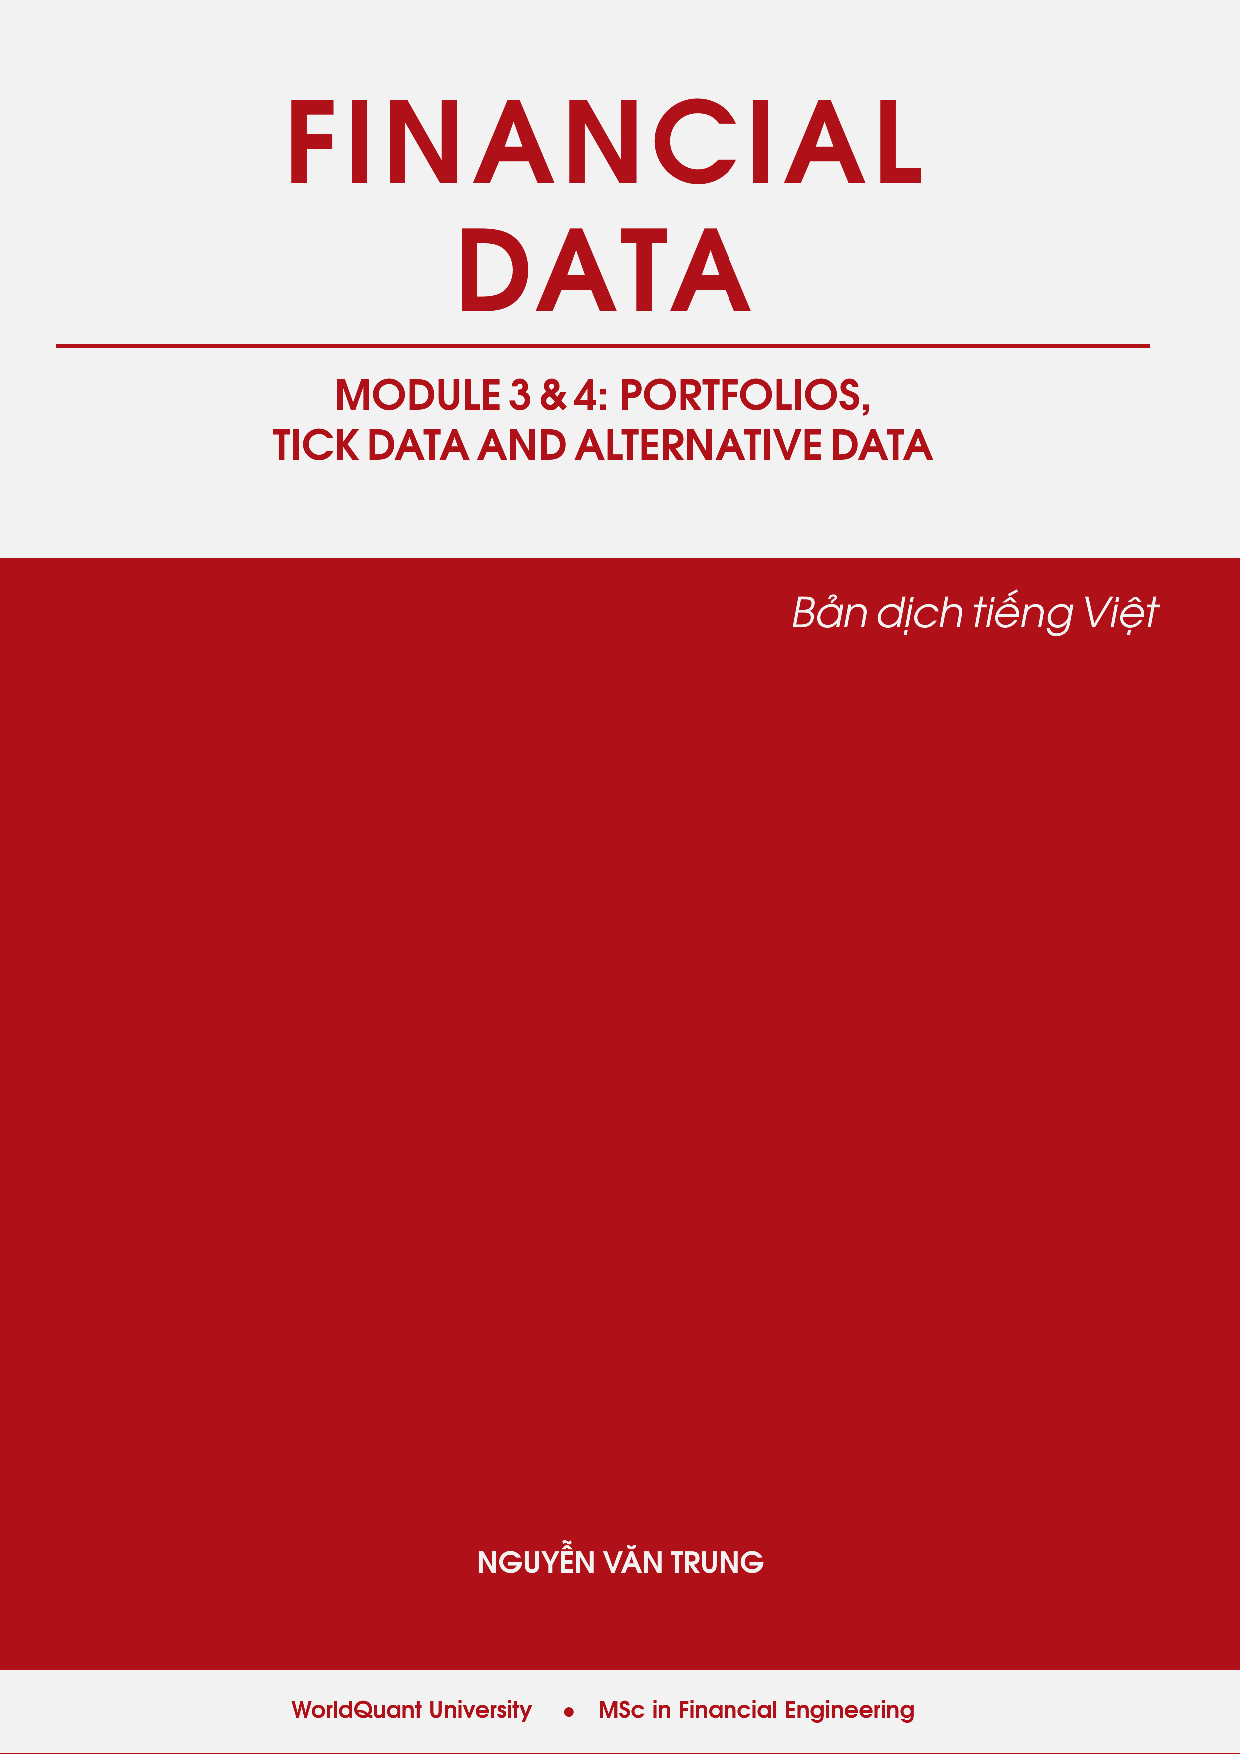
\includepdf[pages=-]{gfx/cover.pdf}}{}
%!TEX root = main-wqu-financial-data-module3-4-dich.tex
% ===================================================================
% DISCLAIMER — Nguồn tài liệu và giấy phép
% ===================================================================

\pdfbookmark[1]{\spacedallcaps{Disclaimer}}{disclaimer}

\thispagestyle{empty}

\section*{Mục đích tài liệu}

Tài liệu này là bản chuyển ngữ cá nhân, được biên soạn phục vụ \textbf{mục đích học tập và nghiên cứu cá nhân} của học viên chương trình Master of Science in Financial Engineering tại WorldQuant University, không nhằm mục đích thương mại và không được phân phối công khai.

Nội dung gồm hai phần:
\begin{itemize}
  \item \textbf{Lesson Notes} do WorldQuant University (WQU) biên soạn cho học viên của khóa học (Module 3 và Module 4).
  \item \textbf{Các bài đọc thêm (Required Readings)} là tài liệu của bên thứ ba. Chỉ phần WQU yêu cầu đọc được dịch sang tiếng Việt, \textbf{sát nguyên bản}, không diễn giải lại hay tóm tắt.
\end{itemize}

Bản dịch là tác phẩm phái sinh: không phải bản chính thức và không được tác giả hay nhà xuất bản của các tài liệu gốc xác nhận. Khi cần trích dẫn hoặc đối chiếu, vui lòng dùng bản gốc tiếng Anh theo các đường dẫn bên dưới.

\section*{Giấy phép của từng tài liệu}

{\small
\renewcommand{\arraystretch}{1.25}
\begin{longtable}{>{\raggedright\arraybackslash}p{0.34\linewidth}>{\raggedright\arraybackslash}p{0.60\linewidth}}
\toprule
\textbf{Tài liệu} & \textbf{Giấy phép / bản quyền} \\
\midrule
\endhead
\textbf{Lesson Notes}, WorldQuant University (Module 3, Module 4). &
Bản quyền © 2024 WorldQuant University. Nội dung chỉ được cấp phép cho mục đích sử dụng cá nhân; nghiêm cấm phân phối lại hoặc xuất bản. \\
\addlinespace
% TODO: bổ sung từng tài liệu đọc thêm (Required Reading) của Module 3 và Module 4 vào đây,
% theo đúng mẫu của module2/disclaimer.tex khi bắt đầu dịch từng Lesson.
\bottomrule
\end{longtable}
}

\section*{Ghi chú}

Hình ảnh và biểu đồ trong các bài đọc thêm được trích trực tiếp từ tài liệu gốc, thuộc cùng phạm vi giấy phép của từng tài liệu; hình trong Lesson Notes là kết quả chạy mã của chính bài học.


\pagestyle{scrheadings}
\tableofcontents
\cleardoublepage
\pagenumbering{arabic}

% ============ MODULE 3: WORKING WITH PORTFOLIOS AND TICK DATA ============

% ---- Lesson 1: Portfolio Returns and Variance ----
% Thứ tự đọc: Lesson Notes -> Đọc thêm
\chapter{Lợi suất và Phương sai Danh mục Đầu tư}
\label{ch:M3L1}

% Lesson: Portfolio Returns and Variance

\section*{Lesson Notes}

MODULE 3 | BÀI 1

{\small
\begin{longtable}{>{\raggedright\arraybackslash}p{0.213\linewidth}>{\raggedright\arraybackslash}p{0.727\linewidth}}
\toprule
\textbf{Thời gian đọc} & 2 giờ \\
\addlinespace[2pt]
\textbf{Kiến thức nền tảng} & Python, lợi suất, phương sai, đa dạng hóa \\
\addlinespace[2pt]
\textbf{Từ khóa} & Lợi suất, logarit, phần trăm, ký hiệu ma trận, phân phối, chuẩn hóa theo năm, trung bình hình học, trung bình số học, phương sai danh mục đầu tư, tương quan, trọng số \\
\addlinespace[2pt]
\bottomrule
\end{longtable}
}

\emph{Trong bài học này, chúng ta sẽ khám phá các loại lợi suất khác nhau, các phương pháp chuẩn hóa lợi suất theo năm, và các kỹ thuật tính phương sai danh mục đầu tư. Bài học nhằm mang lại một hiểu biết toàn diện về cách đo lường và diễn giải hiệu suất danh mục đầu tư, xét trên cả hai khía cạnh lợi suất và rủi ro.}

\emph{Chúng ta sẽ bắt đầu bằng việc xem xét các loại lợi suất khác nhau, bao gồm lợi suất phần trăm và lợi suất logarit, đồng thời thảo luận về đặc tính và trường hợp sử dụng phù hợp của từng loại. Sau đó, chúng ta sẽ chuyển sang các phương pháp chuẩn hóa lợi suất theo năm, điều rất quan trọng khi so sánh các khoản đầu tư qua các khoảng thời gian khác nhau. Bài học cũng sẽ đề cập đến cách tính phương sai danh mục đầu tư, khám phá cách phương sai của từng tài sản, trọng số và tương quan đóng góp vào rủi ro tổng thể của danh mục.}

\section{Lợi suất Danh mục Đầu tư}

Trong môn Thị trường Tài chính, bạn đã được giới thiệu về lợi suất tài sản và lợi suất danh mục đầu tư. Trong Dữ liệu Tài chính, chúng ta sẽ khám phá cả tập dữ liệu một chiều lẫn nhiều chiều. Do đó, biểu diễn ma trận trong đại số tuyến tính sẽ là cánh cửa chính để xử lý chủ đề này. Điều này hợp lý vì một danh mục đầu tư gồm $n$ tài sản với lợi suất $r_{i}, i \in \{1,n\}$ có thể được sắp xếp thành một ma trận $r$ trong đó mỗi cột đại diện cho một tài sản. Trong ngữ cảnh này, $r_{i}$ là các vector, và \textbf{khi không có hiện tượng đa cộng tuyến hoàn hảo}, ta có $\text{dim}(\text{span}(r_{i})) = n$.

Chúng ta đã biết rằng lợi suất danh mục đầu tư là:
$$
r_{p} = \sum_{1}^{n} w_{i} \cdot r_{i}
$$
trong đó
\begin{itemize}
  \item $r_{p}$: lợi suất danh mục đầu tư
  \item $r_{i}$: lợi suất của tài sản $i$
  \item $w_{i}$: trọng số của tài sản $i$
\end{itemize}

Chúng ta cần lưu ý thêm một ràng buộc:
$$
\sum_{1}^{n} w_{i} = 1
$$

và với mục đích của bài học này, chúng ta cũng giả định rằng không được phép bán khống (shorting):
$$
w_{i} > 0
$$

Về bản chất, lợi suất danh mục đầu tư $r_{p}$ là một tổ hợp tuyến tính của lợi suất từng tài sản. Theo cách xây dựng, ta có $r_{p} \in \text{span}(r_{i})$ với mọi tổ hợp trọng số. Điều đó có nghĩa là các tài sản mà nhà đầu tư lựa chọn chính là cơ sở (basis, theo nghĩa Đại số Tuyến tính) của danh mục đầu tư.

Bây giờ hãy viết lợi suất danh mục đầu tư theo định dạng mà chúng ta sẽ sử dụng trong suốt bài học và làm rõ ký hiệu:

$$
r_{p} = \mathbf{r} \cdot \mathbf{w}
$$

với
$$ \mathbf{r} = \begin{bmatrix} r_1 & r_2 & \dots & r_n \end{bmatrix} \text{ , } \mathbf{w} = \begin{bmatrix} w_1 \\ w_2 \\ \vdots \\ w_n \end{bmatrix}$$

và mỗi $r_{i}$ là một vector đại diện cho lợi suất của từng tài sản theo thời gian $t$:
$$
r_{i} = \begin{bmatrix} r^i_{t_{1}} \\ r^i_{t_{2}} \\ \vdots \\ r^i_{t_{m}} \end{bmatrix}
$$

Việc sử dụng $1$ làm tổng của tất cả các trọng số có một cách giải thích trực quan: chúng ta xây dựng danh mục đầu tư bằng cách sử dụng một tỷ lệ phần trăm của mỗi tài sản (các trọng số) cho đến khi dùng hết toàn bộ số vốn ($1$ nghĩa là $100\%$). Vậy điều gì sẽ xảy ra nếu ràng buộc đó bị phá vỡ?

\textbf{Bài tập 1:}

Sử dụng giáo trình tài chính yêu thích của bạn cùng các nguồn trực tuyến để tìm hiểu về ràng buộc $\sum_{1}^{n} w_{i} = 1$. Điều đó sẽ có ý nghĩa gì đối với một danh mục đầu tư nếu $\sum_{1}^{n} w_{i} = 2$? Trả lời câu hỏi tương tự nhưng lần này với $\sum_{1}^{n} w_{i} = 0$. Khởi tạo một chủ đề thảo luận trên diễn đàn để giải thích hiểu biết của bạn.

Hãy tải xuống một số dữ liệu thực tế:

\begin{lstlisting}[language=Python,escapeinside={(*@}{@*)}]
import numpy as np
import pandas as pd
import matplotlib.pyplot as plt
import seaborn as sns
sns.set()
\end{lstlisting}

\begin{lstlisting}[language=Python,escapeinside={(*@}{@*)}]
assets = ['MSFT', 'AAPL', 'AMZN', 'TSLA', 'GOOGL'] # (*@Các@*) (*@tài@*) (*@sản@*) (*@trong@*) (*@danh@*) (*@mục@*)
w = np.array([0.1, 0.2, 0.1, 0.4, 0.2]) # (*@Trọng@*) (*@số@*) (*@của@*) (*@mỗi@*) (*@tài@*) (*@sản@*)

asset_prices = pd.read_csv("portfolio_prices.csv", index_col = "Date", parse_dates = True)

r = asset_prices.pct_change().dropna() # (*@Tính@*) (*@lợi@*) (*@suất@*) (*@phần@*) (*@trăm@*) (*@hàng@*) (*@ngày@*)

r.head() # (*@Mỗi@*) (*@cột@*) (*@là@*) (*@một@*) $r_{i}$
\end{lstlisting}

\begin{lstlisting}[escapeinside={(*@}{@*)}]
                AAPL      AMZN     GOOGL      MSFT      TSLA
Date
2018-01-03 -0.000174  0.012775  0.017061  0.004654 -0.010233
2018-01-04  0.004645  0.004476  0.003884  0.008802 -0.008290
2018-01-05  0.011385  0.016163  0.013260  0.012398  0.006230
2018-01-08 -0.003714  0.014425  0.003531  0.001020  0.062638
2018-01-09 -0.000115  0.004676 -0.001274 -0.000680 -0.008085
\end{lstlisting}

\begin{lstlisting}[language=Python,escapeinside={(*@}{@*)}]
r_port = r @ w # (*@Tạo@*) (*@lợi@*) (*@suất@*) (*@danh@*) (*@mục@*) (*@đầu@*) (*@tư@*)
r_port.name = 'portfolio_returns'
r_port.head()
\end{lstlisting}

\begin{lstlisting}[escapeinside={(*@}{@*)}]
Date
2018-01-03    0.004059
2018-01-04    0.003611
2018-01-05    0.011902
2018-01-08    0.015802
2018-01-09   -0.001093
Name: portfolio_returns, dtype: float64
\end{lstlisting}

\section{Các Loại Lợi suất}

Trong ví dụ trên, chúng ta đã trình bày về bản chất một cách để tính lợi suất phần trăm hàng ngày của danh mục đầu tư. Nhưng đây không phải là loại lợi suất duy nhất được sử dụng trong thực tế:

\subsection{Lợi suất Phần trăm}

Lợi suất phần trăm, còn gọi là lợi suất đơn giản hoặc lợi suất số học, thường được sử dụng trong thực tế:
$$
r_{t} = \frac{p_{t} - p_{t-1}}{p_{t-1}}
$$
trong đó $p_{t}$ là giá của một tài sản tại thời điểm $t$.

Ưu điểm lớn nhất khi sử dụng loại lợi suất này là cách diễn giải trực quan: chúng thể hiện trực tiếp mức thay đổi phần trăm về giá trị. Nhược điểm là chúng không có tính cộng dồn theo thời gian đối với một tài sản, mặc dù chính vì lý do đó mà chúng lại thường được dùng với danh mục đầu tư.

Hệ quả của tính không cộng dồn này khá đơn giản để minh họa: giả sử bạn có một tài sản giá $A$. Tháng đầu tiên, giá tăng $20\%$, nhưng đến cuối tháng thứ hai, giá giảm $18\%$. Nếu lợi suất có tính cộng dồn, ta có thể cộng đơn giản $20\% - 18\% = 2\%$ và cho rằng tổng lợi suất trong 2 tháng là $2\%$. Nhưng như chúng ta sẽ thấy ở phần sau, điều đó không đúng.

Cuối cùng, lợi suất đơn giản không đối xứng. Không có giới hạn trên, nhưng lại có giới hạn dưới. Về mặt trực quan, lợi suất của một cổ phiếu không thể nhỏ hơn $-100\%$ vì giá sẽ trở thành số âm. Ngược lại, ở chiều tăng, lợi suất có thể lên rất cao, đặc biệt khi xét trên khung thời gian dài. Một cách khác để minh họa điều này: giá của một tài sản trong ba tháng liên tiếp là 100 -> 120 -> 100. Cuối tháng thứ hai, lợi suất là $20\%$, nhưng cuối tháng thứ ba, lợi suất là $-16.6\%$. Nếu lợi suất đơn giản đối xứng, thì cần cùng một giá trị tuyệt đối của lợi suất để đi từ 100 lên 120 rồi quay lại 100.

\textbf{Bài tập 2:}

Viết một hàm Python tùy chỉnh, nhận vào một mảng giá (ví dụ \texttt{asset\_prices['MSFT']}), và trả về mảng lợi suất số học. Bạn không được phép sử dụng bất kỳ hàm Python có sẵn nào. Đối chiếu kết quả với kết quả tạo ra bởi hàm \texttt{pct\_change} của pandas.

\subsection{Lợi suất Logarit}

Lợi suất log, còn gọi là lợi suất kép liên tục (continuously compounded returns), sử dụng logarit tự nhiên theo cách sau:

$$
r_{t_\text{log}} = ln \left ( \frac{p_t}{p_{t-1}} \right )
$$

Khác với lợi suất phần trăm, lợi suất log có tính cộng dồn theo thời gian đối với một tài sản:
$$
r_{(t_{i}-t_{j})_{\text{log}}} = \sum_{t = i}^{t = j} r_{t_\text{log}}
$$
chúng cũng thường được giả định (không phải lúc nào cũng đúng) là phân phối chuẩn, một giả định quan trọng cho nhiều mô hình kinh tế lượng và ngẫu nhiên.

Tính cộng dồn này chính là lý do cho tên gọi "lợi suất kép liên tục", vì giờ đây bạn có thể tính tổng lợi suất qua một khoảng thời gian dài chỉ đơn giản bằng cách cộng các lợi suất log trong từng giai đoạn con. Tuy nhiên điều này lại tạo ra một vấn đề: nếu chúng ta có lợi suất logarit riêng lẻ của nhiều tài sản, liệu có hợp lý khi dùng chúng để tính lợi suất của danh mục đầu tư hay không? Nếu việc cộng lợi suất log là một quá trình tính lãi kép, liệu ta có được phép cộng lợi suất log của các tài sản khác nhau?

Câu trả lời cho các câu hỏi trên là \textbf{không}, và ta cần đặc biệt lưu ý để sử dụng đúng loại lợi suất cho từng trường hợp.

Cuối cùng, lợi suất log có tính đối xứng. Về mặt toán học, ta có thể thấy:

$$
log \left ( \frac{p_{t}}{p_{t-1}} \right ) = - log \left ( \frac{p_{t-1}}{p_{t}} \right )
$$

Sử dụng các con số trong ví dụ trên, ta thấy lợi suất log từ 100 lên 120 có giá trị bằng (nhưng ngược dấu) với lợi suất log từ 120 về 100.

\textbf{Bài tập 3:}

Viết một hàm Python tùy chỉnh, nhận vào một mảng giá (ví dụ \texttt{asset\_prices['MSFT']}), và trả về mảng lợi suất logarit.

Như đã minh họa ở trên, chúng ta chỉ có thể phân biệt hai loại lợi suất này dựa trên trường hợp sử dụng. Nhưng bây giờ chúng ta cần cụ thể hơn về thời điểm và cách thức. Để làm điều đó, chúng ta cần thực hiện một quan sát:

\begin{lstlisting}[language=Python,escapeinside={(*@}{@*)}]
print("The 25th quantile is: ", r['MSFT'].quantile(0.25),"\nThe 75th quantile is: ", r['MSFT'].quantile(0.75))
\end{lstlisting}

\begin{lstlisting}[escapeinside={(*@}{@*)}]
The 25th quantile is:  -0.008331217592874807
The 75th quantile is:  0.01093808706491084
\end{lstlisting}

Kết quả trên minh họa rằng, trong nhiều trường hợp, lợi suất hàng ngày có bậc độ lớn khoảng $1\%$. Ngoài ra, đối với lợi suất logarit và lợi suất phần trăm, ta có:
$$
r_{\text{log}} = ln \left ( \frac{p_{t}}{p_{t-1}} \right ) =
ln \left ( \frac{p_{t} - p_{t-1} + p_{t-1}}{p_{t-1}} \right ) =
ln (1 + r_{\text{pct}})
$$

Sử dụng khai triển Taylor cho công thức trên, ta được:
$$
r_{\text{log}} = ln (1 + r_{\text{pct}}) = r_{\text{pct}} - \frac{r_{\text{pct}}^2}{2} + \frac{r_{\text{pct}}^3}{3} - \frac{r_{\text{pct}}^4}{4} + \dots
$$

Vì chúng ta đã quan sát rằng lợi suất hàng ngày nhỏ $< 0.01$, ta có thể giả định rằng các số hạng bậc cao hơn ($r_{\text{pct}}^3$ trở lên) sẽ rất nhỏ:

$$
r_{\text{log}} = r_{\text{pct}} - \frac{r_{\text{pct}}^2}{2} + O(R^3)
$$

Lấy kỳ vọng của cả hai vế trong công thức trên và thực hiện các phép biến đổi đại số, ta có:

$$
\mathbb{E}(r_{\text{log}}) \approx \mathbb{E}(r_{\text{pct}}) - \frac{\sigma^2}{2}
$$
trong đó $\sigma$ là phương sai của lợi suất phần trăm.

Kết quả trên minh họa hai sự thật quan trọng:
\begin{enumerate}
  \item Khi độ biến động thấp, ta kỳ vọng lợi suất log và lợi suất phần trăm sẽ rất gần nhau (Ruppert và Matteson).
  \item Khi tần suất lấy mẫu giảm xuống, lợi suất log và lợi suất phần trăm có xu hướng lớn hơn về giá trị tuyệt đối, và do đó độ biến động cũng có xu hướng tăng lên. Điều này dẫn tới sự phân kỳ giữa hai loại lợi suất.
\end{enumerate}

\begin{lstlisting}[language=Python,escapeinside={(*@}{@*)}]
# Figure 1

pct_returns_msft = asset_prices['MSFT'].pct_change().dropna() # (*@Tính@*) (*@lợi@*) (*@suất@*) (*@phần@*) (*@trăm@*)
log_returns_msft = np.log(asset_prices['MSFT'] / asset_prices['MSFT'].shift(1)).dropna() # (*@Tính@*) (*@lợi@*) (*@suất@*) log

pct_change_msft_roll_mean = pct_returns_msft.rolling(15).mean() # (*@Trung@*) (*@bình@*) (*@trượt@*) (*@của@*) (*@lợi@*) (*@suất@*) (*@phần@*) (*@trăm@*)
log_returns_msft_roll_mean = log_returns_msft.rolling(15).mean() # (*@Trung@*) (*@bình@*) (*@trượt@*) (*@của@*) (*@lợi@*) (*@suất@*) log

fig, ax = plt.subplots(figsize=(12,4))
ax.set_title('Difference between pct and log returns vs Price of MSFT')
ax.plot(asset_prices['MSFT'], label = 'MSFT Price', alpha = 0.7)
ax.set_ylabel('Price')
ax.set_xlabel('Date')
ax.legend()

ax2 = ax.twinx()
ax2.plot((pct_change_msft_roll_mean - log_returns_msft_roll_mean), color = 'red', alpha = 0.5, label = 'Difference between pct and log returns')
ax2.set_ylabel('Difference')
ax2.legend(loc = (0.01,0.89))
plt.show()
\end{lstlisting}

\begin{figure}[H]
\centering
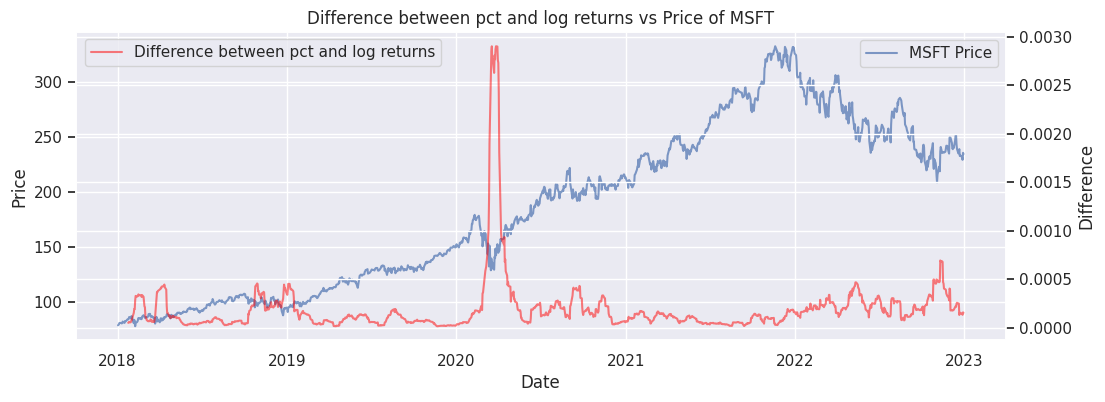
\includegraphics[width=\linewidth,height=0.6\textheight,keepaspectratio]{gfx/m3l1_notes_fig1_pct_vs_log_returns_msft.png}
\par\smallskip{\small \textbf{Hình 1.1:} Chênh lệch giữa lợi suất phần trăm và lợi suất log so với giá MSFT}
\end{figure}

Hình 1.1 minh họa sự chênh lệch giữa lợi suất phần trăm và lợi suất log. Trong các giai đoạn biến động thấp, hai loại lợi suất rất gần nhau, trong khi trong giai đoạn thị trường sụp đổ tháng 3/2020, chênh lệch này trở nên rõ rệt.

\textbf{Bài tập 4:}

MSFT là một cổ phiếu có độ biến động thấp. Hãy tái tạo Hình 1.1 nhưng lần này sử dụng TSLA để minh họa rõ ràng giai đoạn nào hai loại lợi suất phân kỳ.

\textbf{Bài tập 5:}

Hãy lập luận vì sao việc tính trung bình số học có trọng số của lợi suất log của các tài sản khác nhau tại một thời điểm cụ thể sẽ không cho ra lợi suất danh mục đầu tư tại thời điểm đó.

\textbf{Bài tập 6:}

Sử dụng DataFrame \texttt{asset\_prices} đã cho, tính giá trị danh mục đầu tư hàng ngày bằng cách tính tổng có trọng số của giá các tài sản, sử dụng trọng số tài sản đã định trước (như khi tính lợi suất danh mục đầu tư). Tiếp theo, tính lợi suất logarit của chuỗi giá trị danh mục đầu tư này. Thảo luận về các trường hợp sử dụng tiềm năng và ưu điểm của việc dùng lợi suất log trong ngữ cảnh này.

\textbf{Bài tập 7:}

Sử dụng DataFrame \texttt{asset\_prices} đã cho, tính lợi suất lũy kế của mỗi tài sản trong toàn bộ giai đoạn bằng ba phương pháp khác nhau:

\begin{enumerate}
  \item Sử dụng mảng lợi suất phần trăm hàng ngày của mỗi tài sản (gợi ý: bạn sẽ cần dùng hàm \texttt{prod}).
  \item Sử dụng lợi suất log hàng ngày.
  \item Sử dụng mảng giá tài sản.
\end{enumerate}

\section{So sánh Lợi suất Hình học và Số học}

Chúng ta sẽ tiếp tục thảo luận từ Module 2 về cách chuẩn hóa lợi suất theo năm, nhưng trước khi đi sâu vào chủ đề này, chúng ta sẽ xem xét một ví dụ đơn giản minh họa loại trung bình nên được sử dụng cho từng loại lợi suất, \textbf{nếu hiệu ứng lãi kép của lợi suất là cần thiết}.

\subsection{Ví dụ về Trung bình Hình học}

Giả sử tại thời điểm $t_{0}$, bạn có 100 đơn vị. Giữa $t_{0}$ và $t_{1}$, lợi suất của bạn là 20\%, và giữa $t_{1}$ và $t_{2}$, lợi suất là -18\%. Ta giả định các $t_{i}$ cách đều nhau.

\textbf{Tính Trung bình Số học}

Trung bình số học của lợi suất là:

$$
r_{\text{mean}} = \frac{0.2 - 0.18}{2} = 0.01
$$

Điều này cho thấy, trung bình mỗi giai đoạn lợi suất là +1\%. Theo logic này, trong giai đoạn đầu tiên, ta sẽ kiếm được:

$$
100 \cdot 0.01 = 1 \text{ đơn vị}
$$

Vậy, cuối giai đoạn đầu tiên, ta sẽ có 101 đơn vị. Trong giai đoạn thứ hai, giả sử vẫn lợi suất +1\%:

$$
101 \cdot 0.01 = 1.01 \text{ đơn vị}
$$

Điều này ngụ ý rằng cuối giai đoạn thứ hai, ta sẽ có:

$$
100 + 2.01 = 102.01 \text{ đơn vị.}
$$

\textbf{Sử dụng Lợi suất Thực tế}

Bây giờ, hãy áp dụng cách tiếp cận khác bằng việc áp dụng lợi suất thực tế lần lượt.

\begin{enumerate}
  \item Cuối $t_{1}$, với lợi suất 20\% trên 100 đơn vị:

$$
100 \cdot 0.2 = 20 \text{ đơn vị kiếm được.}
$$

  Vậy, bạn có 120 đơn vị cuối $t_{1}$.

  \item Trong giai đoạn thứ hai, từ $t_{1}$ đến $t_{2}$, lợi suất là -18\%. Bắt đầu với 120 đơn vị:

$$
120 \times 0.18 = 21.6 \text{ đơn vị mất đi.}
$$

  Vậy, cuối $t_{2}$, bạn có:

$$
120 - 21.6 = 98.4 \text{ đơn vị.}
$$
\end{enumerate}

\textbf{Phương pháp nào đúng?}

Hãy tính trung bình hình học để xem phương pháp nào phản ánh đúng thực tế:

$$
r_{\text{GeomMean}} = \left(\prod _{i=1}^{n} (1 + r_{i}) \right)^{\frac {1}{n}} - 1
$$

Với hai giai đoạn của chúng ta:

$$
r_{\text{GeomMean}} = \left( (1 + 0.2) \cdot (1 - 0.18) \right)^{\frac{1}{2}} - 1 = \sqrt{1.2 \cdot 0.82} - 1 \approx 0.992 - 1 = -0.008
$$

Bây giờ hãy kiểm chứng trung bình hình học này xem nó có phản ánh đúng giá trị cuối cùng hay không:

$$
100 \cdot (1 - 0.008) \cdot (1 - 0.008) \approx 100 \cdot 0.992 \cdot 0.992 = 98.4 \text{ đơn vị.}
$$

Ví dụ này minh họa một điều hiển nhiên: khoản lỗ 18\% trên 120 đơn vị lớn hơn khoản lãi 20\% trên 100 đơn vị, dẫn đến sự sụt giảm giá trị tổng thể. Do đó, mặc dù trung bình số học gợi ý một lợi suất dương 1\%, thực tế bạn đã mất tiền, như trung bình hình học đã cho thấy. Trung bình hình học phản ánh chính xác hơn lợi suất kép qua nhiều giai đoạn, đặc biệt khi lợi suất biến động.

Tất nhiên đây là khi ta xét một tài sản qua thời gian chứ không phải khi xét nhiều tài sản tại một thời điểm cụ thể.

\subsection{Trung bình Số học}

Chúng ta đã xác định rằng không thể dùng trung bình số học với lợi suất phần trăm cho một tài sản qua thời gian \textbf{nếu hiệu ứng lãi kép quan trọng đối với phân tích} (trừ khi độ biến động thực sự thấp như đã giải thích). Vậy câu hỏi là, liệu ta có thể dùng trung bình số học với lợi suất logarit hay không? Hãy viết lại ví dụ trên bằng lợi suất logarit thay vì lợi suất đơn giản.

Lợi suất log là:

$$
r_{\text{log}_1} = \log(1.2) \approx 0.1823, \quad r_{\text{log}_2} = \log(0.82) \approx -0.1987
$$

Vì lợi suất log có tính cộng dồn, ta có thể tổng hợp lợi suất như sau:

$$
r_{\text{ArithMean}} = \frac{1}{2} \left ( r_{\text{log}_1} + r_{\text{log}_2} \right ) =\frac{1}{2} \left ( \log(1.2) + \log(0.82) \right )
$$

Theo tính chất của logarit:

$$
r_{\text{ArithMean}} = \frac{1}{2} \log(1.2 \cdot 0.82) \approx \log(0.984^{\frac{1}{2}}) \approx \log(0.992)
$$

Lấy hàm mũ cho ra lợi suất kép thực tế:

$$
\exp(\log(0.992)) = 0.992
$$

Kết quả này trùng với trung bình hình học, đúng phản ánh giá trị cuối cùng:

$$
100 \cdot 0.992 \cdot 0.992 \approx 98.4 \text{ đơn vị.}
$$

Như vậy, trung bình số học $r_{\text{ArithMean}}$ của lợi suất log cho ra lợi suất trung bình \emph{đúng}, phù hợp với lãi kép thực tế.

\textbf{Bài tập 8:}

Sử dụng các tính chất của logarit, hãy chứng minh rằng lợi suất log thực sự là lợi suất kép liên tục. (Gợi ý: $r^{t_{1}}_{\text{log}} + r^{t_{2}}_{\text{log}} + r^{t_{3}}_{\text{log}} + \dots = ln \left ( \frac{p_{t_{2}}}{p_{t_{1}}} \right ) + ln \left ( \frac{p_{t_{3}}}{p_{t_{2}}} \right ) + \dots$). Hãy chứng minh rằng:

$$
ln(r_{\text{GeomMean}} + 1) = \frac{1}{n}\sum_{t=1}^{t=n} r^{t}_{\text{log}}
$$

Hãy kiểm chứng Bài tập 8 bằng dữ liệu thực tế:

\begin{lstlisting}[language=Python,escapeinside={(*@}{@*)}]
percent_returns_tsla = asset_prices['TSLA'].loc["2020-06-01":"2020-09-30"].pct_change().dropna() # (*@Tính@*) (*@lợi@*) (*@suất@*) (*@phần@*) (*@trăm@*) (*@hàng@*) (*@ngày@*)
geom_mean_tsla_1 = ((1 + percent_returns_tsla).prod() ** (1/len(percent_returns_tsla))) - 1 # (*@Tính@*) (*@trung@*) (*@bình@*) (*@hình@*) (*@học@*)

log_returns_tsla = np.log(asset_prices['TSLA'].loc["2020-06-01":"2020-09-30"] / asset_prices['TSLA'].loc["2020-06-01":"2020-09-30"].shift(1)).dropna() # (*@Tính@*) (*@lợi@*) (*@suất@*) log (*@hàng@*) (*@ngày@*)
arithmetic_mean_tsla_1 = log_returns_tsla.mean() # (*@Tính@*) (*@trung@*) (*@bình@*) (*@số@*) (*@học@*)

print("Logarithm of geometric Mean of TSLA + 1: ", np.log(geom_mean_tsla_1 + 1))
print("Arithmetic Mean of TSLA: ", arithmetic_mean_tsla_1)
\end{lstlisting}

\begin{lstlisting}[escapeinside={(*@}{@*)}]
Logarithm of geometric Mean of TSLA + 1:  0.010242784447195914
Arithmetic Mean of TSLA:  0.010242784447195901
\end{lstlisting}

\subsection{Chọn Đúng Loại Trung bình cho Lợi suất Phần trăm}

Khi phân tích lợi suất đầu tư, việc chọn đúng loại trung bình phù hợp với ngữ cảnh là điều thiết yếu. Trung bình số học là \textbf{thước đo đúng để tính lợi suất kỳ vọng trong các mô hình thống kê và tối ưu hóa danh mục đầu tư}. Nó thể hiện lợi suất trung bình mỗi giai đoạn mà không xét đến hiệu ứng lãi kép. Điều này rất quan trọng khi dự báo lợi suất tương lai, tính lợi suất danh mục kỳ vọng, và thực hiện đánh giá rủi ro, vì nó phù hợp với các tính chất tuyến tính cần thiết trong các phép tính này.

Mặt khác, trung bình hình học phản ánh chính xác tốc độ tăng trưởng kép trung bình qua nhiều giai đoạn. Nó tính đến hiệu ứng lãi kép và phù hợp để đánh giá hiệu suất lịch sử của một khoản đầu tư theo thời gian. Tuy nhiên, không nên dùng trung bình hình học thay cho trung bình số học khi thực hiện phân tích thống kê hoặc mô hình hóa lợi suất kỳ vọng, vì nó không cho ra ước lượng không thiên lệch (unbiased) về hiệu suất tương lai.

Tóm lại, trong khi trung bình hình học vô cùng hữu ích để hiểu mức tăng trưởng thực tế của một khoản đầu tư nhờ lãi kép, trung bình số học vẫn là thước đo nền tảng trong các bối cảnh thống kê và quản lý danh mục đầu tư khi đánh giá lợi suất kỳ vọng và ra quyết định đầu tư.

\section{Chuẩn hóa Lợi suất Phần trăm theo Năm}

Các ví dụ trên (phần lớn khá đơn giản) được dùng để tạo trực giác rằng bạn cần phân biệt giữa việc chuẩn hóa lợi suất logarit và lợi suất phần trăm theo năm. Chuẩn hóa lợi suất theo năm là điều thiết yếu vì nó cho phép ta so sánh các khoản đầu tư qua các khoảng thời gian khác nhau trên cùng một cơ sở hàng năm. Quá trình này thiết yếu để đánh giá hiệu suất và so sánh các tài sản khác nhau.

Đối với lợi suất phần trăm, ta dùng trung bình hình học để tính đến hiệu ứng lãi kép. Công thức chuẩn hóa lợi suất phần trăm hàng ngày theo năm là:

$$
R_{\text{Annual}} = (1 + r_{\text{GeomMean}})^N - 1
$$

Trong đó:

\begin{itemize}
  \item $R_{\text{Annual}}$ là lợi suất đã chuẩn hóa theo năm
  \item $N$ là số kỳ giao dịch trong một năm (có thể là 252 ngày hoặc 12 tháng đối với cổ phiếu, hoặc 365 ngày đối với các tài sản giao dịch liên tục, v.v.)
\end{itemize}

\section{Chuẩn hóa Lợi suất Logarit theo Năm}

Đối với lợi suất logarit, việc chuẩn hóa theo năm đơn giản hơn nhờ tính cộng dồn của chúng. Công thức chuẩn hóa lợi suất log hàng ngày theo năm là:

$$
R_{\text{Annual,Log}} = N \cdot r_{\text{ArithMean}}
$$

Nếu muốn chuyển đổi trở lại thành lợi suất năm "thực tế", ta có:

$$
R_{\text{Annual}} = e^{N \cdot r_{\text{ArithMean}}} - 1
$$

Hãy tính lợi suất năm của MSFT.

\begin{lstlisting}[language=Python,escapeinside={(*@}{@*)}]
geom_mean_msft = ((1 + pct_returns_msft).prod() ** (1/len(pct_returns_msft))) - 1 # (*@Tính@*) (*@trung@*) (*@bình@*) (*@hình@*) (*@học@*)
annual_pct_returns_msft = (1 + geom_mean_msft) ** 252 - 1 # (*@Chuẩn@*) (*@hóa@*) (*@lợi@*) (*@suất@*) (*@phần@*) (*@trăm@*) theo (*@năm@*)

annual_log_returns_msft = log_returns_msft.mean() * 252 # (*@Chuẩn@*) (*@hóa@*) (*@lợi@*) (*@suất@*) log theo (*@năm@*)

print("Annualized pct returns of MSFT: ", annual_pct_returns_msft)
print("Annualized log returns of MSFT: ", annual_log_returns_msft)
\end{lstlisting}

\begin{lstlisting}[escapeinside={(*@}{@*)}]
Annualized pct returns of MSFT:  0.24306555153098586
Annualized log returns of MSFT:  0.21758054768754312
\end{lstlisting}

\textbf{Bài tập 9:}

Tính lợi suất năm cho TSLA, cả với lợi suất phần trăm lẫn lợi suất log.

\section{Phương sai Danh mục Đầu tư}

\subsection{Tổng quan về Phương sai Danh mục Đầu tư}

Nội dung này đã được thảo luận ở mức tổng quan trong môn Thị trường Tài chính, nhưng ở đây, chúng ta sẽ minh họa cách tính phương sai trong Python với dữ liệu thực nghiệm. Trong khi lợi suất quan trọng, nhà đầu tư cũng quan tâm đến rủi ro, hay độ biến động.

Nhưng hãy suy nghĩ một chút về cách chúng ta có thể đo lường rủi ro cho một danh mục gồm $n$ tài sản. Nếu chỉ có một tài sản, ta có thể tính độ lệch chuẩn của lợi suất và điều này cho ta một ước lượng về mức độ lợi suất lệch khỏi lợi suất trung bình. Tương tự, ta có thể lập luận rằng ta có thể tính lợi suất danh mục đầu tư rồi sau đó tính độ lệch chuẩn.

\begin{lstlisting}[language=Python,escapeinside={(*@}{@*)}]
r_port.std() # (*@Tính@*) (*@độ@*) (*@lệch@*) (*@chuẩn@*) (*@của@*) (*@lợi@*) (*@suất@*) (*@danh@*) (*@mục@*) (*@đầu@*) (*@tư@*)
\end{lstlisting}

\begin{lstlisting}[escapeinside={(*@}{@*)}]
np.float64(0.020274896364979554)
\end{lstlisting}

Trong môn Thị trường Tài chính, ta cũng biểu diễn phương sai danh mục đầu tư như sau:

$$
\sigma^{2}_{p} = \sum_{i=1}^{n} \sum_{j=1}^{n} w_i w_j \text{Cov}(r_i, r_j)
$$

Trong đó:

\begin{itemize}
  \item $w_i$ = trọng số danh mục của tài sản thứ $i$
  \item $\text{Cov}_{i,j}$ = hiệp phương sai giữa hai tài sản, có thể biểu diễn dưới dạng $\rho_{_{(i,j)}} \sigma_i \sigma_j$, trong đó $\rho_{_{(i,j)}}$ là hệ số tương quan giữa hai tài sản
\end{itemize}

Công thức dưới đây tương đương với công thức trên, nhưng được viết dưới dạng ma trận:

$$
\sigma^{2}_{p} = \mathbf{w}^{T} \cdot \Sigma \cdot \mathbf{w}
$$

Trong đó $\Sigma$ là ma trận hiệp phương sai của danh mục đầu tư.

\begin{lstlisting}[language=Python,escapeinside={(*@}{@*)}]
port_var = w.T @ r.cov() @ w # (*@Tính@*) (*@phương@*) (*@sai@*) (*@danh@*) (*@mục@*) (*@đầu@*) (*@tư@*)
port_std = np.sqrt(port_var) # (*@Tính@*) (*@độ@*) (*@lệch@*) (*@chuẩn@*) (*@danh@*) (*@mục@*) (*@đầu@*) (*@tư@*)

print("Portfolio variance: ", port_var)
print("Portfolio standard deviation: ", port_std)
\end{lstlisting}

\begin{lstlisting}[escapeinside={(*@}{@*)}]
Portfolio variance:  0.0004110714226106612
Portfolio standard deviation:  0.020274896364979554
\end{lstlisting}

Trong ô lệnh trên, chúng ta đã cho thấy cách tính phương sai danh mục đầu tư một cách trực quan và đơn giản (bằng cách tính trực tiếp độ lệch chuẩn trên giá trị danh mục) có thể được tái tạo bằng cách sử dụng ma trận hiệp phương sai và các trọng số. Về bản chất, những gì chúng ta đã làm là phân rã phương sai danh mục đầu tư thành nhiều thành phần:
\begin{itemize}
  \item Các trọng số
  \item Các phương sai riêng lẻ
  \item Các hiệp phương sai giữa từng cặp
\end{itemize}

Kết quả trên phần nào đã được dự đoán trước. Nếu phương sai của một tài sản đột ngột thay đổi, phương sai danh mục đầu tư sẽ thay đổi. Nếu trọng số của một tài sản có phương sai cao thay đổi, ta kỳ vọng phương sai danh mục cũng sẽ thay đổi tương ứng. Nhưng còn hiệp phương sai thì sao?

Để thấy rõ hơn, chúng ta sẽ phân rã ma trận hiệp phương sai thêm một chút:

$$
\Sigma = D \cdot R \cdot D
$$

trong đó

\begin{itemize}
  \item D là ma trận đường chéo chứa độ lệch chuẩn của từng tài sản
  \item R là ma trận tương quan
\end{itemize}

Phân rã cuối cùng này cho thấy rằng phương sai danh mục đầu tư cũng phụ thuộc vào các tương quan (Pearson) theo từng cặp.

\subsection{Ảnh hưởng của Tương quan lên Phương sai Danh mục Đầu tư}

Hãy viết phương sai danh mục đầu tư dưới dạng toàn phương (quadratic form) nhưng sử dụng tương quan thay vì hiệp phương sai:

$$
\sigma_p^2 = \sum_{i=1}^{n} w_i^2 \sigma_i^2 + \sum_{i=1}^{n}\sum_{j \neq i}^{n} w_i w_j \sigma_{ij}
$$

Thay $\sigma_{ij} = \rho_{ij} \sigma_i \sigma_j$, ta có:

$$
\sigma_p^2 = \sum_{i=1}^{n} w_i^2 \sigma_i^2 + \sum_{i=1}^{n}\sum_{j \neq i}^{n} w_i w_j \rho_{ij} \sigma_i \sigma_j
$$

Để hiểu phương sai danh mục đầu tư thay đổi thế nào theo tương quan $\rho_{ij}$, ta lấy đạo hàm riêng của $\sigma_p^2$ theo $\rho_{ij}$:

$$
\frac{\partial \sigma_p^2}{\partial \rho_{ij}} = \frac{\partial}{\partial \rho_{ij}} \left( \sum_{i=1}^{n} w_i^2 \sigma_i^2 + \sum_{i=1}^{n}\sum_{j \neq i}^{n} w_i w_j \rho_{ij} \sigma_i \sigma_j \right)
$$

Tổng đầu tiên độc lập với $\rho_{ij}$, nên đạo hàm của nó theo $\rho_{ij}$ bằng 0. Đạo hàm của tổng thứ hai, theo $\rho_{ij}$, cho ta:

$$
\frac{\partial \sigma_p^2}{\partial \rho_{ij}} = w_i w_j \sigma_i \sigma_j
$$

Chúng ta đã giả định rằng $w_{i} > 0$ và ta biết rằng độ lệch chuẩn luôn dương. Điều đó có nghĩa là:

$$
\frac{\partial \sigma_p^2}{\partial \rho_{ij}} > 0
$$

Giữ các yếu tố khác không đổi, nếu tương quan giữa hai tài sản tăng/giảm, phương sai danh mục đầu tư sẽ tăng/giảm. Do đó, nếu tương quan của nhiều tài sản tăng cùng lúc, phương sai danh mục đầu tư sẽ tăng nhanh hơn, và đó có thể là dấu hiệu của rủi ro hệ thống.

Hãy minh họa một số điều trên với dữ liệu thực tế:

\begin{lstlisting}[language=Python,escapeinside={(*@}{@*)}]
# Figure 2
# (*@Chúng@*) ta (*@sẽ@*) (*@trực@*) quan (*@hóa@*) (*@độ@*) (*@lệch@*) (*@chuẩn@*) (*@và@*) (*@lợi@*) (*@suất@*) (*@của@*) (*@tài@*) (*@sản@*) (*@so@*) (*@với@*) (*@danh@*) (*@mục@*)

fig, (ax1, ax2) = plt.subplots(1, 2, figsize = (14,4))

ax1.bar(x = r.columns, height = r.std(), alpha = 0.7)
ax1.hlines(y = port_std, xmin = -0.4, xmax = 4.4, linestyle = "--", color = 'red', alpha = 0.8, label = "Portfolio Std")
ax1.set_title("Assets vs Portfolio Volatlity")
ax1.set_ylabel("Volatility")
ax1.legend()

ax2.bar(x = r.columns, height = (r + 1).prod() - 1, alpha = 0.7) # (*@Đảm@*) (*@bảo@*) (*@bạn@*) (*@có@*) (*@thể@*) (*@giải@*) (*@thích@*) (*@vì@*) sao `(r + 1).prod() - 1` (*@là@*) (*@tổng@*) (*@lợi@*) (*@suất@*)
ax2.hlines(y = (r_port + 1).prod() - 1, xmin = -0.4, xmax = 4.4, linestyle = "--", color = 'red', alpha = 0.8, label = "Portfolio Total Returns")
ax2.set_title("Assets vs Portfolio Total Returns")
ax2.set_ylabel("Total Returns (* 100%)")
ax2.legend()

plt.show()
\end{lstlisting}

\begin{figure}[H]
\centering
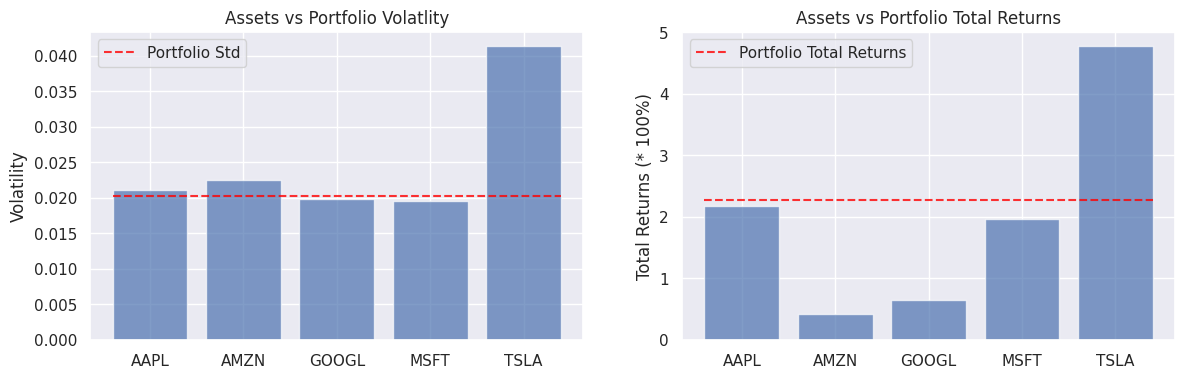
\includegraphics[width=\linewidth,height=0.6\textheight,keepaspectratio]{gfx/m3l1_notes_fig2_assets_vs_portfolio_volatility_returns.png}
\par\smallskip{\small \textbf{Hình 1.2:} Độ lệch chuẩn và tổng lợi suất của từng tài sản so với danh mục đầu tư}
\end{figure}

Trong Hình 1.2, các trọng số chúng ta chọn (ngẫu nhiên) cho ra một danh mục có độ biến động gần với phần lớn các tài sản, nhưng lợi suất lại cao hơn hẳn.

Hãy kiểm tra mối quan hệ giữa phương sai danh mục đầu tư với phương sai của một tài sản ngẫu nhiên, ví dụ MSFT.

\begin{lstlisting}[language=Python,escapeinside={(*@}{@*)}]
# Figure 3
multipliers = np.linspace(0.1,5,100) # (*@Tạo@*) (*@một@*) (*@mảng@*) (*@dùng@*) (*@để@*) (*@nhân@*) (*@với@*) (*@mảng@*) (*@lợi@*) (*@suất@*) MSFT
portfolio_variances = []
msft_variances = []

for multiplier in multipliers:
  temp_returns = r * np.array([1, 1, 1, multiplier, 1]) # (*@Nhân@*) (*@lợi@*) (*@suất@*) MSFT (*@với@*) (*@một@*) (*@con@*) (*@số@*) (*@để@*) (*@thay@*) (*@đổi@*) (*@tuyến@*) (*@tính@*) (*@lợi@*) (*@suất@*), (*@qua@*) (*@đó@*) (*@thay@*) (*@đổi@*) (*@phương@*) (*@sai@*) (*@của@*) MSFT
  temp_port_variance = w.T @ temp_returns.cov() @ w # (*@Tính@*) (*@phương@*) (*@sai@*) (*@danh@*) (*@mục@*) (*@đầu@*) (*@tư@*)
  msft_variances.append((temp_returns['MSFT']).var())
  portfolio_variances.append(temp_port_variance)
  assert np.allclose(r.corr(), temp_returns.corr()) # (*@Với@*) (*@mỗi@*) (*@mảng@*) (*@lợi@*) (*@suất@*) (*@mới@*) (*@mà@*) (*@lợi@*) (*@suất@*) MSFT (*@được@*) (*@nhân@*) (*@với@*) (*@một@*) (*@số@*), (*@các@*) (*@tương@*) (*@quan@*) (*@vẫn@*) (*@giữ@*) (*@nguyên@*)

fig, (ax1, ax2) = plt.subplots(1, 2, figsize = (16,5))

ax1.plot(multipliers, portfolio_variances)
ax1.scatter(1, port_var, color = 'red', label = "Initial Portfolio Variance (non scaled MSFT returns)")
ax1.set_title("Portfolio Variance as MSFT variance is increasing")
ax1.set_xlabel("Multiplier")
ax1.set_ylabel("Variance")
ax1.legend()

ax2.plot(multipliers[10:30], portfolio_variances[10:30])
ax2.scatter(1, port_var, color = 'red', label = "Initial Portfolio Variance (non scaled MSFT returns)")
ax2.plot(multipliers[10:30], msft_variances[10:30], color = 'purple', label = "MSFT Variance (non scaled MSFT returns)")
ax2.set_title("Portfolio Variance vs MSFT variance")
ax2.set_xlabel("Multiplier")
ax2.set_ylabel("Variance")
ax2.legend()

plt.show()
\end{lstlisting}

\begin{figure}[H]
\centering
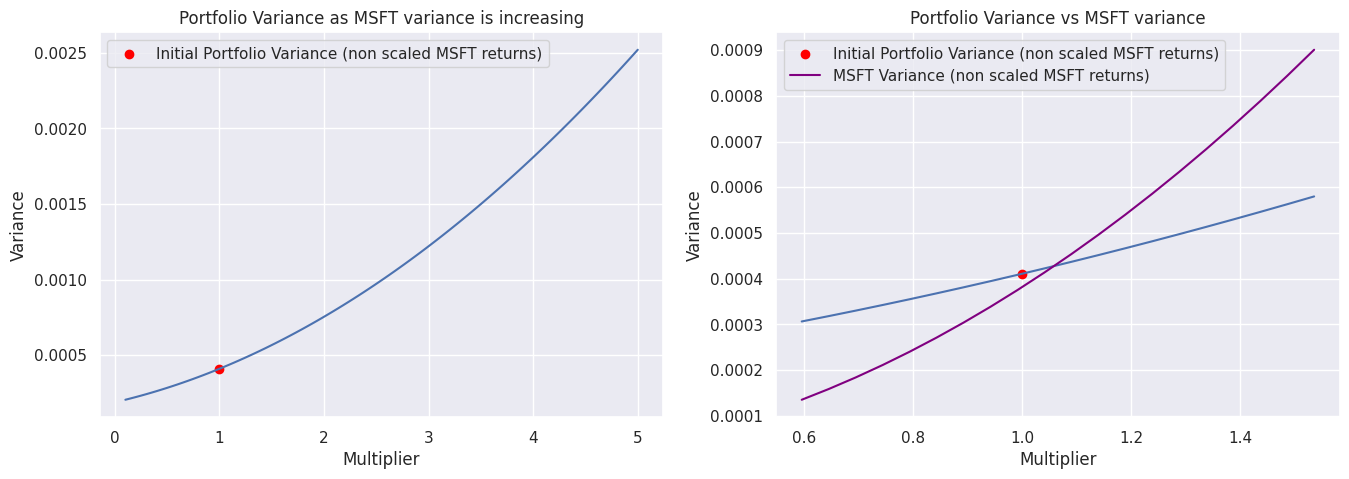
\includegraphics[width=\linewidth,height=0.6\textheight,keepaspectratio]{gfx/m3l1_notes_fig3_portfolio_variance_vs_asset_variance.png}
\par\smallskip{\small \textbf{Hình 1.3:} Phương sai danh mục đầu tư khi phương sai của MSFT tăng dần, so với phương sai của MSFT}
\end{figure}

Hình 1.3 minh họa ảnh hưởng của việc tăng phương sai một tài sản (ở đây là MSFT) lên phương sai danh mục đầu tư. Như dự đoán, mối quan hệ giữa phương sai danh mục đầu tư và phương sai của bất kỳ tài sản nào là bậc hai (đồ thị bên trái). Đồ thị bên phải minh họa sự khác biệt về rủi ro khi nắm giữ một tài sản duy nhất so với nắm giữ cả danh mục đầu tư.

Trong ví dụ tiếp theo, chúng ta giữ nguyên phương sai và trọng số, và xem xét tương quan ảnh hưởng thế nào đến phương sai danh mục đầu tư. Chúng ta giả định $100$ tài sản và xây dựng các ma trận tương quan với tương quan đồng nhất theo từng cặp — nghĩa là mọi cặp tài sản đều có cùng hệ số tương quan. Sự đơn giản hóa này cho phép ta tách biệt ảnh hưởng thuần túy của độ lớn tương quan lên rủi ro danh mục đầu tư. Chúng ta sẽ thử nghiệm $19$ mức tương quan khác nhau, từ $0$ (các tài sản hoàn toàn không tương quan) đến $0.8$ (các tài sản tương quan cao). Lưu ý rằng với $100$ tài sản, các giá trị tương quan nhỏ hơn khoảng $-0.01$ sẽ tạo ra các ma trận tương quan không hợp lệ về mặt toán học (không xác định dương), nên chúng ta tập trung vào phạm vi thực tế từ 0 đến tương quan dương mạnh, đại diện cho các điều kiện thị trường điển hình — từ danh mục đầu tư đa dạng hóa tốt đến các tình huống rủi ro hệ thống cao khi tất cả tài sản có xu hướng di chuyển cùng nhau.

\begin{lstlisting}[language=Python,escapeinside={(*@}{@*)}]
n_assets = 100
w = np.random.dirichlet(np.ones(n_assets), size=1)[0]

degrees_of_freedom = 8
variances = np.random.chisquare(df=degrees_of_freedom, size=n_assets)
variances = variances / np.max(variances) * 0.003
std_devs = np.sqrt(variances)
D = np.diag(std_devs)

# (*@Bắt@*) (*@đầu@*) (*@từ@*) (*@gần@*) (*@bằng@*) (*@0@*) (*@đến@*) (*@tương@*) (*@quan@*) (*@dương@*) (*@cao@*) ((*@phạm@*) (*@vi@*) (*@thực@*) (*@tế@*) (*@của@*) (*@thị@*) (*@trường@*))
correlation_values = np.linspace(0, 0.8, 19)

corr_matrices = []
portfolio_variances = []

for corr in correlation_values:
    # (*@Tạo@*) (*@ma@*) (*@trận@*) (*@tương@*) (*@quan@*) (*@đồng@*) (*@nhất@*)
    R = np.full((n_assets, n_assets), corr)
    np.fill_diagonal(R, 1)

    corr_matrices.append(R)

    # (*@Tính@*) (*@phương@*) (*@sai@*) (*@danh@*) (*@mục@*) (*@đầu@*) (*@tư@*)
    portfolio_variance = w.T @ D @ R @ D @ w
    portfolio_variances.append(portfolio_variance)

# (*@Vẽ@*) (*@biểu@*) (*@đồ@*)
plt.figure(figsize=(10, 5))
plt.plot(correlation_values, portfolio_variances, 'b-o', linewidth=2, markersize=6)
plt.title("Portfolio Variance vs Correlation\n(100 assets, realistic correlation range)")
plt.xlabel("Uniform Pairwise Correlation")
plt.ylabel("Portfolio Variance")
plt.grid(True, alpha=0.3)
plt.xlim(-0.05, 0.85)

plt.show()

print(f"Portfolio variance increases {portfolio_variances[-1]/portfolio_variances[0]:.1f}x as correlation goes from {correlation_values[0]} to {correlation_values[-1]}")
\end{lstlisting}

\begin{lstlisting}[escapeinside={(*@}{@*)}]
Portfolio variance increases 32.7x as correlation goes from 0.0 to 0.8
\end{lstlisting}

\begin{figure}[H]
\centering
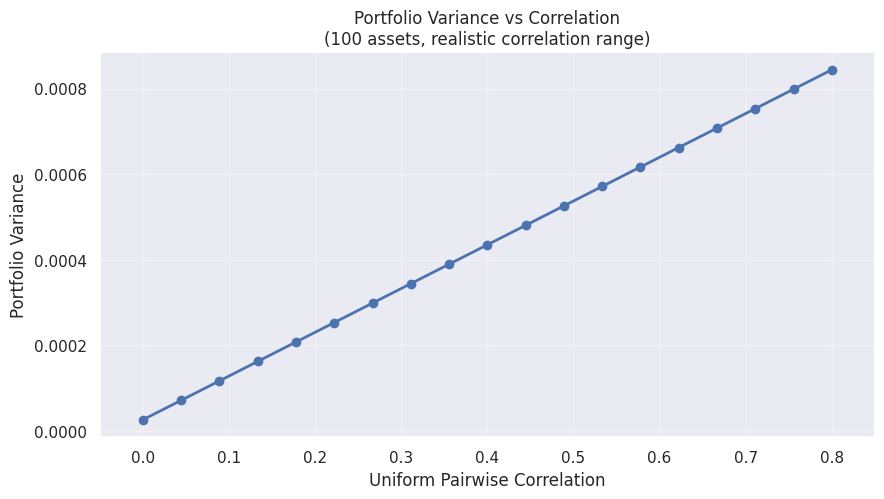
\includegraphics[width=\linewidth,height=0.6\textheight,keepaspectratio]{gfx/m3l1_notes_fig4_portfolio_variance_vs_correlation.png}
\par\smallskip{\small \textbf{Hình 1.4:} Phương sai danh mục đầu tư theo tương quan (100 tài sản, phạm vi tương quan thực tế)}
\end{figure}

Những học viên chưa có nền tảng tài chính có thể không ngờ tới kết quả này. Ngay cả khi phương sai từng tài sản và trọng số không đổi, sự thay đổi trong tương quan vẫn ảnh hưởng mạnh mẽ đến phương sai danh mục đầu tư. Cụ thể trong ví dụ này, phương sai danh mục đầu tư thấp nhất khi tương quan bằng 0 (các tài sản không tương quan), và tăng tuyến tính khi tương quan trở nên dương hơn. Với tương quan $0.8$, phương sai danh mục đầu tư cao gấp khoảng $36$ lần so với khi tương quan bằng 0. Điều này minh họa nguyên lý nền tảng của đa dạng hóa: kết hợp các tài sản không tương quan giúp giảm rủi ro hiệu quả hơn nhiều so với kết hợp các tài sản tương tự, có tương quan cao. Mối quan hệ tuyến tính quan sát được (với tương quan đồng nhất) sẽ trở nên phức tạp hơn khi cấu trúc tương quan thực tế hơn, nhưng thông điệp cốt lõi vẫn đúng — khi các tài sản tương quan cao hơn, lợi ích đa dạng hóa giảm dần và rủi ro danh mục tăng lên. Điều này giải thích tại sao các cuộc khủng hoảng thị trường lại nguy hiểm đối với các danh mục đầu tư đa dạng hóa: trong giai đoạn căng thẳng, tương quan có xu hướng tăng vọt lên gần $1$, khiến các danh mục tưởng chừng đa dạng hóa tốt lại hành xử gần như một tài sản đơn lẻ.

\textbf{Bài tập 10:}

Chọn $n \geq 2$ cổ phiếu/trái phiếu và xây dựng một danh mục đầu tư (chọn trọng số phù hợp) sử dụng dữ liệu lịch sử sao cho phương sai danh mục bằng $0$ (hoặc thực sự gần $0$ để được coi là $0$) và lợi suất dương (khác xa $0$). Trình bày phát hiện của bạn trên diễn đàn. Nếu bạn không tìm được, hãy trình bày lý do vì sao không tìm được.

\section{Trọng số Danh mục Đầu tư}

Giả sử ta có thể xây dựng một danh mục đầu tư gồm cổ phiếu, trái phiếu và tiền điện tử. Một nhà đầu tư có thể chọn nắm giữ nhiều trái phiếu trong khi người khác chọn chủ yếu cổ phiếu và người thứ ba lại yêu thích tiền điện tử. Sự lựa chọn này liên quan đến hồ sơ rủi ro của nhà đầu tư; nói cách khác, việc chọn trọng số sẽ đáp ứng nhu cầu về lợi suất cụ thể với một mức chấp nhận rủi ro (phương sai) nhất định.

Từ góc nhìn này, việc chọn trọng số là một vấn đề mang tính chủ quan, và trên thực tế, các nhà đầu tư hành xử rất khác nhau (Elton et al.). Một trong những cách tốt nhất để khám phá điều này là xây dựng đồ thị Đường biên Hiệu quả (Efficient Frontier).

\begin{lstlisting}[language=Python,escapeinside={(*@}{@*)}]
from scipy.optimize import minimize

weights = np.random.dirichlet(np.ones(5)*0.7, size = 20000) # (*@Tạo@*) 20000 (*@bộ@*) (*@trọng@*) (*@số@*) (*@sử@*) (*@dụng@*) (*@phân@*) (*@phối@*) dirichlet

assert np.isclose(np.sum(weights, axis = 1), 1).all() # (*@Kiểm@*) (*@tra@*) (*@mỗi@*) (*@bộ@*) (*@trọng@*) (*@số@*) (*@có@*) (*@tổng@*) (*@bằng@*) 1

eff_front_dict = {}
cov_matrix_ret = r.cov() * 252
expected_returns = r.mean() * 252

# (*@Điền@*) (*@vào@*) eff_front_dict
for w in weights:
  port_ret = expected_returns @ w.T # (*@Lợi@*) (*@suất@*) (*@kỳ@*) (*@vọng@*) (*@chuẩn@*) (*@hóa@*) theo (*@năm@*)
  port_std = np.sqrt(w.T @ cov_matrix_ret @ w)
  eff_front_dict[str(list(w))] = [port_ret, port_std]

eff_frontier_dataframe = pd.DataFrame(eff_front_dict, index = ['Returns', 'Standard Deviation']).T # (*@Lưu@*) (*@mọi@*) (*@thứ@*) (*@vào@*) (*@một@*) dataframe

def get_portfolio_stats(weights, expected_returns, cov_matrix):
    port_ret = expected_returns @ weights
    port_std = np.sqrt(weights.T @ cov_matrix @ weights)
    return port_ret, port_std

def negative_sharpe_ratio(weights, expected_returns, cov_matrix, risk_free_rate=0.02):
    port_ret, port_std = get_portfolio_stats(weights, expected_returns, cov_matrix)
    sharpe_ratio = (port_ret - risk_free_rate) / port_std
    return -sharpe_ratio

def minimum_variance(weights, expected_returns, cov_matrix):
    return get_portfolio_stats(weights, expected_returns, cov_matrix)[1]

def efficient_frontier_point(expected_returns, cov_matrix, target_return):
    n_assets = len(expected_returns)
    args = (expected_returns, cov_matrix)
    constraints = (
        {'type': 'eq', 'fun': lambda w: np.sum(w) - 1},
        {'type': 'eq', 'fun': lambda w: get_portfolio_stats(w, expected_returns, cov_matrix)[0] - target_return}
    )
    bounds = tuple((0, 1) for _ in range(n_assets))

    result = minimize(
        minimum_variance,
        x0=np.ones(n_assets) / n_assets,
        args=args,
        method='SLSQP',
        bounds=bounds,
        constraints=constraints
    )

    return result.x

def get_efficient_frontier(expected_returns, cov_matrix, n_points=100):
    # (*@Tìm@*) (*@danh@*) (*@mục@*) (*@phương@*) (*@sai@*) (*@nhỏ@*) (*@nhất@*)
    n_assets = len(expected_returns)
    args = (expected_returns, cov_matrix)
    constraints = ({'type': 'eq', 'fun': lambda w: np.sum(w) - 1})
    bounds = tuple((0, 1) for _ in range(n_assets))

    min_var_result = minimize(
        minimum_variance,
        x0=np.ones(n_assets) / n_assets,
        args=args,
        method='SLSQP',
        bounds=bounds,
        constraints=constraints
    )
    min_ret, min_std = get_portfolio_stats(min_var_result.x, expected_returns, cov_matrix)

    # (*@Tìm@*) (*@danh@*) (*@mục@*) (*@lợi@*) (*@suất@*) (*@lớn@*) (*@nhất@*)
    max_ret_idx = np.argmax(expected_returns)
    max_ret = expected_returns[max_ret_idx]

    # (*@Tạo@*) (*@các@*) (*@điểm@*) (*@trên@*) (*@đường@*) (*@biên@*) (*@hiệu@*) (*@quả@*)
    target_returns = np.linspace(min_ret, max_ret, n_points)
    efficient_portfolios = []

    for target_return in target_returns:
        weights = efficient_frontier_point(expected_returns, cov_matrix, target_return)
        ret, std = get_portfolio_stats(weights, expected_returns, cov_matrix)
        efficient_portfolios.append([std, ret])

    return np.array(efficient_portfolios)

# (*@Tính@*) (*@các@*) (*@điểm@*) (*@của@*) (*@đường@*) (*@biên@*) (*@hiệu@*) (*@quả@*)
efficient_points = get_efficient_frontier(expected_returns, cov_matrix_ret)

# (*@Vẽ@*) (*@biểu@*) (*@đồ@*)
plt.figure(figsize=(10,6))
plt.scatter(x=eff_frontier_dataframe['Standard Deviation'],
           y=eff_frontier_dataframe['Returns'],
           alpha=0.4)
plt.scatter(x=r.std() * np.sqrt(252),
           y=expected_returns,
           color='red',
           label="Individual Assets",
           alpha=0.7)
plt.plot(efficient_points[:,0],
         efficient_points[:,1],
         'orange',
         linewidth=3,
         label='Efficient Frontier',
         alpha=0.6)
plt.title("Efficient Frontier")
plt.xlabel("Annual Portfolio Standard Deviation")
plt.ylabel("Annual Portfolio Returns")
plt.legend()
plt.grid(True)
plt.show()
\end{lstlisting}

\begin{figure}[H]
\centering
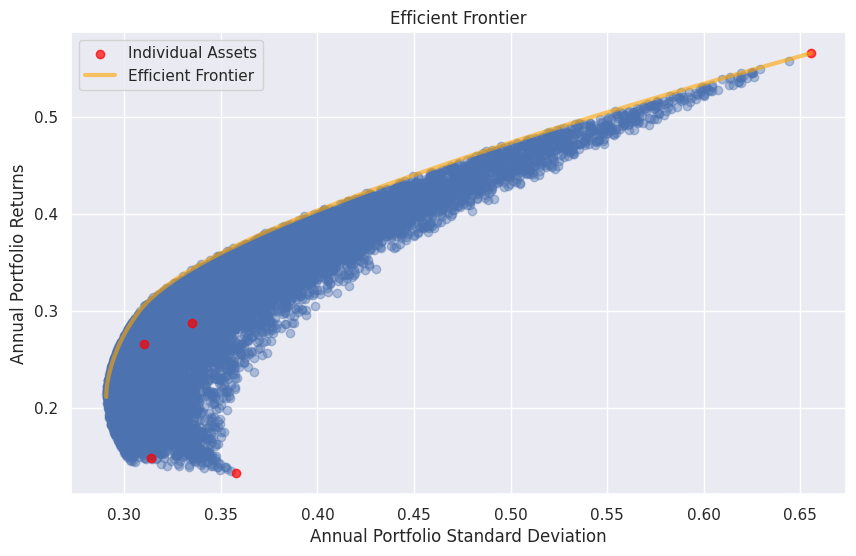
\includegraphics[width=\linewidth,height=0.6\textheight,keepaspectratio]{gfx/m3l1_notes_fig5_returns_vs_risk_portfolios.png}
\par\smallskip{\small \textbf{Hình 1.5:} Đường biên Hiệu quả (Efficient Frontier) của danh mục đầu tư gồm 5 tài sản}
\end{figure}

Hãy đọc hiểu minh họa trên, được thừa nhận là một trong những đồ thị quan trọng nhất trong quản lý danh mục đầu tư.

Trước hết, ta cần quan sát hình dạng của đường biên: đường cong trải dài ở phần trên bên trái của biểu đồ phân tán đại diện cho tất cả các danh mục đầu tư tối ưu khả dĩ, mang lại lợi suất kỳ vọng cao nhất cho một mức rủi ro cho trước (hoặc rủi ro thấp nhất cho một mức lợi suất kỳ vọng cho trước). Đường cong này được gọi là \textbf{đường biên hiệu quả} (efficient frontier).

Thứ hai, nếu vẽ các đường thẳng đứng trên đồ thị này, mỗi đường sẽ cắt đường biên tại một điểm đại diện cho danh mục có lợi suất cao nhất ứng với mức rủi ro cụ thể đó. Đồng thời, có rất nhiều bộ trọng số khiến danh mục chịu cùng mức rủi ro nhưng lợi suất thấp hơn. Điều đó nên khiến ta chú ý rằng mặc dù trọng số mang tính chủ quan, nếu danh mục mà nhà đầu tư chọn không nằm trên đường biên hiệu quả, thì nhà đầu tư có thể đạt lợi suất tốt hơn bằng cách đi theo đường thẳng đứng lên trên cho đến khi chạm đường biên hiệu quả. Nói ngắn gọn, với bất kỳ mức rủi ro (phương sai) nào, luôn tồn tại một cấu trúc danh mục tối ưu tối đa hóa lợi suất.

Điều tương tự cũng đúng nếu ta vẽ các đường ngang. Trong trường hợp này, ta có thể khẳng định rằng với bất kỳ mức lợi suất nào, ta có thể tối thiểu hóa rủi ro bằng cách đi theo đường ngang sang trái cho đến khi cắt đường biên hiệu quả.

Khi di chuyển lên trên và sang phải dọc theo đường biên, ta thấy lợi suất tiềm năng cao hơn nhưng cũng rủi ro cao hơn. Điều này minh họa nguyên lý nền tảng rằng để đạt lợi suất cao hơn, nhìn chung ta phải chấp nhận rủi ro cao hơn. Hình dạng lõm của đường biên minh họa lợi ích của đa dạng hóa. Các danh mục nằm trên đường biên thường được đa dạng hóa tốt, mang lại hồ sơ rủi ro-lợi suất tốt hơn so với từng tài sản riêng lẻ.

\textbf{Bài tập 11:}

Xây dựng danh mục đầu tư của riêng bạn, theo sở thích của bạn: chọn một hoặc nhiều cổ phiếu, ETF, trái phiếu và tiền điện tử. Cố gắng bao gồm các tài sản không tương quan nhiều với phần còn lại của danh mục (nếu có thể) và cũng bao gồm một số tài sản có độ biến động rất cao (altcoin vốn hóa lớn hoặc mới phát hành). Sử dụng mã đã cung cấp ở trên để xây dựng đường biên hiệu quả. Dán đồ thị lên diễn đàn cùng với một đoạn văn \textbf{ngắn} liệt kê các tài sản đã chọn.

\textbf{Bài tập 12 (Tùy chọn):}

Trong đoạn đầu tiên của notebook này, chúng ta đã đề cập rằng với $n$ vector $r_{i}$, khi không có đa cộng tuyến, ta có $\text{dim}(\text{span}(r_{i})) = n$. Ngược lại, số chiều của $\text{span}$ sẽ thấp hơn $n$. Đây là một kết quả đã biết trong đại số tuyến tính. Hãy dùng giáo trình đại số tuyến tính yêu thích của bạn để ôn lại khái niệm đa cộng tuyến, sau đó lập luận vì sao một nhà đầu tư vẫn giữ một tài sản trong danh mục khi tài sản đó có thể được viết dưới dạng tổ hợp tuyến tính hoàn hảo của các tài sản còn lại trong danh mục. Nhà đầu tư có nên loại bỏ tài sản đó không? Đóng góp của nó vào việc giảm phương sai danh mục hoặc tăng lợi suất là gì? Nó có mang lại sự linh hoạt trong quản lý danh mục hay không?

\textbf{Bài tập 13:}

Xuyên suốt bài học này, học viên đã được giới thiệu cách sử dụng đúng trung bình số học và trung bình hình học. Trong mục \emph{2.4 Chuẩn hóa Lợi suất theo Năm}, chúng ta đã giải thích cách chuẩn hóa lợi suất phần trăm và lợi suất log theo năm nếu cần hiệu ứng lãi kép. Tuy nhiên, khi xây dựng đường biên hiệu quả, ta đã làm như sau: \texttt{expected\_returns = r.mean() * 252}. Tại sao? Trong câu trả lời của bạn, hãy xem xét bối cảnh tối ưu hóa danh mục đầu tư và liệu ta đang tập trung mô hình hóa lợi suất kỳ vọng cho mục đích thống kê hay tính mức tăng trưởng lịch sử thực tế của một khoản đầu tư do lãi kép. Thảo luận về hệ quả của việc sử dụng trung bình số học trong ngữ cảnh này.

\section{Kết luận}

Trong bài học này, chúng ta đã học rằng lợi suất logarit có tính cộng dồn và hữu ích cho phân tích dài hạn, trong khi lợi suất phần trăm trực quan hơn cho đánh giá hiệu suất ngắn hạn. Chúng ta cũng đã tìm hiểu cách chuẩn hóa lợi suất theo năm, cho phép so sánh công bằng giữa các khoản đầu tư có khung thời gian khác nhau.
Bài học nhấn mạnh tầm quan trọng của việc hiểu phương sai danh mục đầu tư và các thành phần của nó. Chúng ta đã thấy phương sai từng tài sản, trọng số và tương quan đều đóng vai trò quan trọng trong việc xác định rủi ro tổng thể của danh mục. Khái niệm đường biên hiệu quả minh họa sự đánh đổi giữa rủi ro và lợi suất, làm nổi bật lợi ích của đa dạng hóa.

Thông qua các ví dụ và bài tập thực hành bằng Python, chúng ta đã có kinh nghiệm thực tế trong việc tính toán và diễn giải các chỉ số này. Kiến thức này tạo nền tảng thiết yếu cho các chủ đề nâng cao hơn trong quản lý danh mục đầu tư và phân tích tài chính.

\textbf{Tài liệu tham khảo}

\begin{itemize}
  \item Elton, Edwin J., et al. \emph{Modern Portfolio Theory and Investment Analysis}. John Wiley \& Sons, 2009.
  \item Ruppert, David, and David S. Matteson. \emph{Statistics and Data Analysis for Financial Engineering}. 2nd ed., Springer, 2011.
\end{itemize}

\chapter{Đọc thêm: Rủi ro và Lợi suất (Dahlquist \& Knight)}
\label{ch:M3L1-reading1}

% Nguồn: Dahlquist, Julie, and Rainford Knight. "Principles of Finance." OpenStax, 2022.
% Phần cần đọc: Sections 15.1 (Risk and Return to an Individual Asset) & 15.2 (Risk and Return to Multiple Assets)
% Nội dung bắt buộc đọc: được kiểm tra trong mọi bài đánh giá (kể cả Quiz).

\section{Thông tin nguồn}

\begin{itemize}
  \item \textbf{Nguồn:} Dahlquist, Julie, and Rainford Knight. \emph{Principles of Finance}. OpenStax Press, 2022. (truy cập mở tại \url{https://openstax.org/details/books/principles-finance})
  \item \textbf{Phần cần đọc:} Section 15.1: Risk and Return to an Individual Asset; Section 15.2: Risk and Return to Multiple Assets
\end{itemize}

\section{15.1 Rủi ro và Lợi suất của Một Tài sản Riêng lẻ}

\subsection*{Mục tiêu học tập}
Sau khi hoàn thành mục này, bạn sẽ có thể:
\begin{itemize}
  \item Tính lợi suất thực hiện (realized return) từ một khoản đầu tư riêng lẻ.
  \item Tính lợi suất trung bình và độ biến động của lợi suất từ dữ liệu lịch sử.
  \item Mô tả rủi ro đặc thù doanh nghiệp (firm-specific risk).
\end{itemize}

\subsection*{Đo lường Lợi suất Lịch sử}

Rủi ro và lợi suất thường được gọi là hai chữ R (the two Rs) của tài chính. Nhà đầu tư quan tâm đến cả rủi ro lẫn lợi suất vì hiểu một cái mà không hiểu cái kia thì thực sự vô nghĩa. Về mặt đầu tư, khái niệm lợi suất khá đơn giản: lợi suất là lợi ích, hay lợi nhuận, mà nhà đầu tư kỳ vọng từ một khoản chi tiêu. Đó là phần thưởng cho việc đầu tư — lý do khiến một khoản đầu tư được thực hiện ngay từ đầu. Tuy nhiên, không có khoản đầu tư nào là chắc chắn. Lợi suất thực tế có thể không như nhà đầu tư kỳ vọng. Sự không chắc chắn về lợi suất này được gọi là rủi ro.

Chúng ta bắt đầu bằng cách xem xét cách đo lường cả rủi ro lẫn lợi suất khi xét một tài sản riêng lẻ, chẳng hạn một cổ phiếu. Nếu ông bà bạn mua 100 cổ phiếu Apple, Inc. cho bạn khi bạn mới sinh ra, bạn sẽ muốn biết khoản đầu tư đó đã sinh lời tốt đến đâu. Bạn thậm chí có thể muốn so sánh khoản đầu tư đó với một khoản đầu tư vào một cổ phiếu khác, chẳng hạn Disney, xem cái nào tốt hơn. Bạn quan tâm đến việc đo lường lợi suất lịch sử.

\subsection*{Lợi suất Thực hiện của Khoản đầu tư Riêng lẻ}

Lợi suất thực hiện (realized return) của một khoản đầu tư là tổng lợi suất xảy ra trong một khoảng thời gian cụ thể. Giả sử bạn mua một cổ phiếu Target (TGT) vào đầu tháng 1/2020 với giá \$128.74. Đến cuối năm, bạn bán cổ phiếu với giá \$176.53, cao hơn \$47.79 so với giá mua. Mức tăng giá trị này được gọi là lãi vốn (capital gain). Là chủ sở hữu cổ phiếu, bạn cũng nhận được \$2.68 cổ tức trong năm 2020. Tổng lợi suất bằng đô la từ khoản đầu tư của bạn được tính như sau:

$$
\text{Tổng lợi suất} = \$47.79 + \$2.68 = \$50.47
$$

Lợi suất đầu tư thường được biểu diễn theo phần trăm thay vì đô la. Điều này cho phép bạn trả lời câu hỏi "Tôi nhận được bao nhiêu cho mỗi đô la đầu tư?" để có thể so sánh các khoản đầu tư có quy mô khác nhau. Tổng lợi suất phần trăm từ khoản đầu tư của bạn là:

$$
\text{Tổng lợi suất \%} = \frac{\$50.47}{\$128.74} = 39.20\%
$$

Tỷ suất cổ tức (dividend yield) được tính bằng cách chia cổ tức nhận được cho giá cổ phiếu ban đầu. Phép tính này cho thấy với mỗi đô la đầu tư vào TGT năm 2020, bạn nhận được \$0.0208 tiền cổ tức. Tỷ suất lãi vốn (capital gain yield) là mức thay đổi giá cổ phiếu chia cho giá cổ phiếu ban đầu. Phép tính này cho thấy với mỗi đô la đầu tư vào TGT năm 2020, bạn nhận được \$0.3712 lãi vốn. Tổng lợi suất phần trăm 39.20\% của bạn có nghĩa là bạn kiếm được \$0.392 cho mỗi đô la đầu tư khi cộng cả lợi nhuận từ cổ tức lẫn tăng giá cổ phiếu.

\begin{framed}
\textbf{THỰC HÀNH: Tính Lợi suất}

Bạn mua 10 cổ phiếu 3M (MMM) vào tháng 1/2020 với giá \$175/cổ phiếu, nhận cổ tức \$5.91/cổ phiếu, và bán cổ phiếu vào cuối năm với giá \$169.72/cổ phiếu. Hãy tính tổng lợi suất bằng đô la, tỷ suất cổ tức, tỷ suất lãi vốn, và tổng lợi suất phần trăm.

\textbf{Lời giải:}

Vì bạn mua 10 cổ phiếu, bạn nhận được $10 \times \$5.91 = \$59.10$ tiền cổ tức. Bạn chi $10 \times \$175 = \$1{,}750$ để mua cổ phiếu, và bán được $10 \times \$169.72 = \$1{,}697.20$. Tổng lợi suất bằng đô la của bạn là $\$1{,}697.20 - \$1{,}750 + \$59.10 = \$6.30$.

Tỷ suất cổ tức của bạn là $\$59.10 / \$1{,}750 = 3.38\%$, và tỷ suất lãi vốn là $(\$1{,}697.20 - \$1{,}750)/\$1{,}750 = -3.02\%$. Tổng lợi suất phần trăm của bạn là $3.38\% - 3.02\% = 0.36\%$.

Lưu ý rằng bạn đã bán MMM với giá thấp hơn giá mua đầu năm. Lãi vốn của bạn âm, hay còn gọi là lỗ vốn (capital loss). Dù giá giảm, bạn vẫn có tổng lợi suất bằng đô la dương nhờ khoản thu nhập từ cổ tức.
\end{framed}

Tất nhiên, nhà đầu tư hiếm khi mua một cổ phiếu rồi bán đúng một năm sau. Giả sử bạn mua cổ phiếu Facebook (FB) vào ngày 1/6/2020 với giá \$228.50/cổ phiếu và bán ba tháng sau với giá \$261.90. Bạn không nhận cổ tức nào. Trong trường hợp này, lợi suất phần trăm theo kỳ nắm giữ (holding period) được tính là:

$$
\frac{\$261.90 - \$228.50}{\$228.50} = 14.62\%
$$

Con số 14.62\% này là lợi suất cho kỳ nắm giữ ba tháng. Để so sánh với các cơ hội đầu tư khác, bạn cần biểu diễn lợi suất theo cơ sở hàng năm, hay chuẩn hóa theo năm. Lợi suất theo kỳ nắm giữ được chuyển đổi thành tỷ lệ hàng năm hiệu dụng (effective annual rate — EAR) bằng công thức:

$$
EAR = (1 + \text{Lợi suất theo kỳ})^{m} - 1
$$

trong đó $m$ là số kỳ nắm giữ trong một năm.

Có bốn kỳ ba tháng trong một năm. Vậy EAR cho khoản đầu tư này là:

$$
EAR = (1.1462)^{4} - 1 = 71.87\%
$$

Điều gì xảy ra nếu bạn sở hữu một cổ phiếu hơn một năm? Lợi suất theo kỳ nắm giữ của bạn khi đó sẽ xảy ra trong khoảng thời gian dài hơn một năm, nhưng quy trình tính EAR vẫn như vậy. Giả sử bạn mua cổ phiếu FB vào tháng 5/2015, khi giá là \$79.30/cổ phiếu. Bạn giữ cổ phiếu đến tháng 5/2020, khi bán với giá \$224.59. Lợi suất phần trăm theo kỳ nắm giữ của bạn sẽ là $(\$224.59-\$79.30)/\$79.30 = 183.21\%$. Bạn đã hơn gấp ba số tiền của mình, nhưng mất năm năm để làm được điều đó. EAR của bạn, vốn sẽ nhỏ hơn tỷ lệ lợi suất theo kỳ nắm giữ năm năm này, được tính là:

$$
EAR = (1 + 1.8321)^{1/5} - 1 = 23.13\%
$$

\subsection*{Lợi suất Trung bình Hàng năm}

Giả sử bạn mua cổ phiếu Delta Airlines (DAL) vào đầu năm 2011 với giá \$11.19 và giữ cổ phiếu trong 10 năm trước khi bán với giá \$40.21. Bạn kiếm được $(\$40.21-\$11.19)/\$11.19 = 259.34\%$ trên khoản đầu tư của mình trong giai đoạn 10 năm. Đây là lợi suất theo kỳ nắm giữ 259.34\%. EAR cho khoản đầu tư này được tính bằng cách trước tiên tính lợi suất theo kỳ nắm giữ. Lợi suất theo kỳ nắm giữ thể hiện phần trăm lợi suất kiếm được trong suốt thời gian nắm giữ khoản đầu tư. Sau đó, lợi suất theo kỳ nắm giữ được chuyển đổi thành tỷ lệ phần trăm hàng năm bằng công thức đã nêu.

Bạn cũng có thể dùng công thức giá trị thời gian của tiền (time value of money) cơ bản để tính EAR của một khoản đầu tư. Trong ngôn ngữ giá trị thời gian của tiền, giá ban đầu trả cho khoản đầu tư, \$11.19, là giá trị hiện tại (present value). Giá bán cổ phiếu, \$40.21, là giá trị tương lai (future value). Phải mất 10 năm để \$11.19 tăng lên \$40.21. Sử dụng giá trị thời gian của tiền sẽ cho ra kết quả tính toán:

$$
EAR = \left( \frac{40.21}{11.19} \right)^{1/10} - 1 = 13.65\%
$$

Công thức EAR và công thức giá trị thời gian của tiền đều cho ra lợi suất hàng năm 13.65\%. Về mặt toán học, hai công thức là giống nhau; công thức này chỉ là một cách sắp xếp đại số khác của công thức kia.

Nếu bạn kiếm được 13.65\% mỗi năm, lãi kép trong 10 năm, bạn sẽ chuyển đổi khoản đầu tư \$11.19/cổ phiếu thành \$40.21/cổ phiếu. Tất nhiên, cổ phiếu DAL không tăng đúng 13.65\% mỗi năm. Lợi suất của DAL cho mỗi năm được trình bày trong Bảng 15.1. Có những năm, lợi suất cao hơn nhiều so với 13.65\%. Năm 2013, lợi suất gần 133\%! Những năm khác, lợi suất thấp hơn nhiều so với 13.65\%; thực tế, lợi suất âm trong bốn năm.

\begin{figure}[H]
\centering
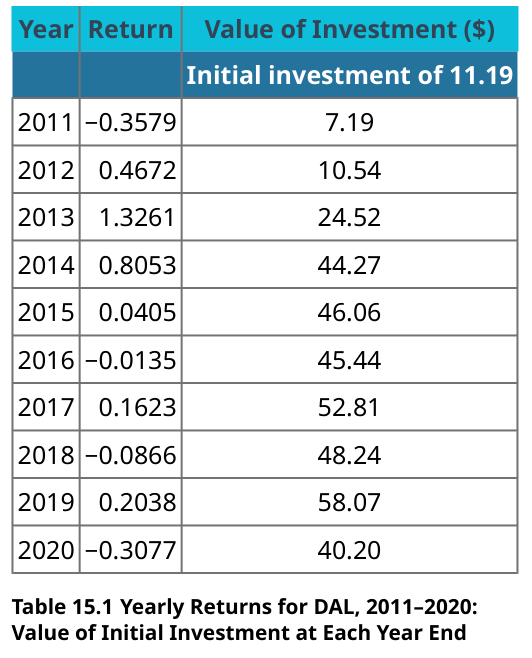
\includegraphics[width=0.7\linewidth]{gfx/m3l1_dahlquist_table15-1_dal_investment_value.png}
\par\smallskip{\small \textbf{Bảng 15.1:} Lợi suất hàng năm của DAL, 2011--2020: Giá trị khoản đầu tư ban đầu vào cuối mỗi năm}
\end{figure}

Mặc dù khoản đầu tư \$11.19 vào DAL đầu năm 2011 đã tăng lên \$40.20 vào cuối năm 2020, mức tăng trưởng này không nhất quán qua từng năm. Số tiền cổ phiếu đáng giá vào cuối mỗi năm cũng được trình bày trong Bảng 15.1. Trong năm 2011, lợi suất của DAL là $-35.79\%$, khiến giá trị khoản đầu tư giảm xuống $\$11.19 \times (1-0.3579) = \$7.19$. Năm tiếp theo, 2012, lợi suất của DAL là 46.72\%. Do đó, giá trị khoản đầu tư là $\$7.19 \times (1+0.4672) = \$10.54$ vào cuối năm 2012. Quá trình này tiếp diễn qua từng năm cổ phiếu được nắm giữ.

Lợi suất hàng năm kép suy ra từ công thức EAR và giá trị thời gian của tiền còn được gọi là lợi suất trung bình hình học (geometric average return). Lợi suất trung bình hình học được tính bằng công thức:

$$
R_{\text{GeomAvg}} = \left[ (1+R_1)(1+R_2)\cdots(1+R_N) \right]^{1/N} - 1
$$

trong đó $R_N$ là lợi suất của mỗi năm trong giai đoạn tính trung bình.

Phép tính lợi suất trung bình hình học cho DAL được trình bày ở cột bên phải của Bảng 15.2. (Chênh lệch nhỏ giữa lợi suất trung bình hình học 13.64\% với 13.65\% suy ra từ EAR và giá trị thời gian của tiền là do sai số làm tròn.)

\begin{figure}[H]
\centering
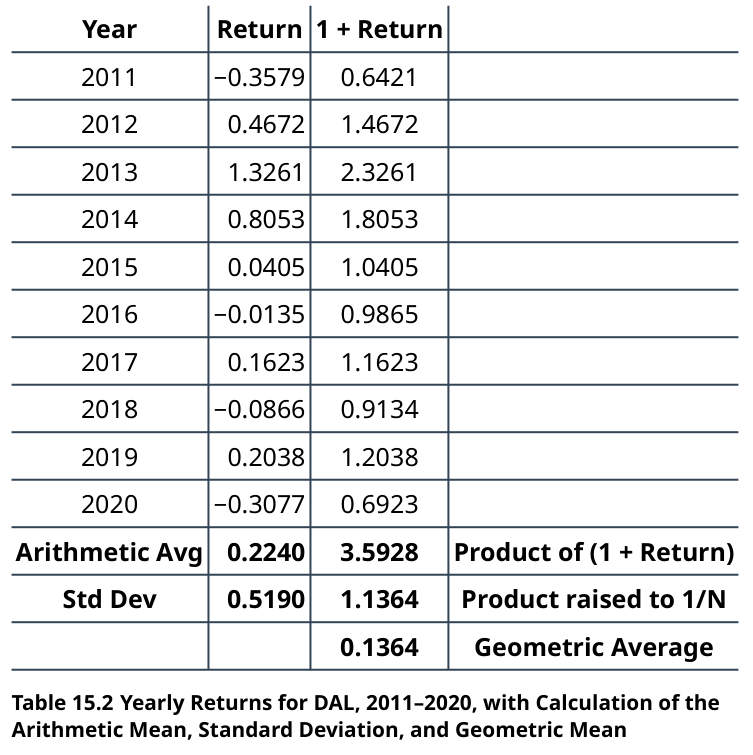
\includegraphics[width=0.75\linewidth]{gfx/m3l1_dahlquist_table15-2_dal_geometric_avg.png}
\par\smallskip{\small \textbf{Bảng 15.2:} Lợi suất hàng năm của DAL, 2011--2020, cùng phép tính Trung bình Số học, Độ lệch chuẩn và Trung bình Hình học}
\end{figure}

Nhìn vào Bảng 15.2, bạn sẽ nhận thấy lợi suất trung bình hình học khác với lợi suất trung bình (mean). Cộng từng lợi suất hàng năm và chia tổng cho 10 cho ra lợi suất trung bình hàng năm là 22.4\%. Con số 22.4\% này được gọi là lợi suất trung bình số học (arithmetic average return).

Lợi suất trung bình hình học sẽ nhỏ hơn lợi suất trung bình số học (trừ khi lợi suất của tất cả các năm giống hệt nhau). Điều này là do bản chất số học cơ bản của lãi kép. Hãy nghĩ về một ví dụ rất đơn giản trong đó bạn đầu tư \$100 trong hai năm. Nếu năm đầu tiên bạn có lợi suất dương 50\% và năm thứ hai lợi suất âm 50\%, bạn sẽ có lợi suất trung bình số học là $(50\%-50\%)/2 = 0\%$, nhưng bạn sẽ có lợi suất trung bình hình học là $[(1.5)(0.5)]^{1/2}-1 = -13.40\%$. Với lợi suất dương 50\% năm đầu tiên, bạn kết thúc năm với \$150. Năm thứ hai, bạn mất 50\% số dư đó và chỉ còn lại \$75.

Một sự thật quan trọng khác khi nghiên cứu lợi suất trung bình là thứ tự bạn kiếm được các lợi suất đó không quan trọng. Hãy xem xét điều gì sẽ xảy ra nếu lợi suất của hai năm bị đảo ngược, tức là bạn chịu lỗ 50\% trong năm đầu tư đầu tiên và lãi 50\% trong năm thứ hai. Với lợi suất $-50\%$ năm đầu tiên, bạn sẽ kết thúc năm đó chỉ với \$50. Sau đó, nếu \$50 đó sinh lợi 50\% dương ở năm thứ hai, bạn sẽ có số dư \$75 vào cuối giai đoạn hai năm. Lợi suất âm 50\% theo sau bởi lợi suất dương 50\% vẫn cho ra lợi suất trung bình số học 0\% và lợi suất trung bình hình học $-13.40\%$.

\begin{framed}
\textbf{THỰC HÀNH: Tính Lợi suất Trung bình Số học và Hình học}

Lợi suất hàng năm của CVS Health Corp. (CVS) cho giai đoạn 10 năm 2011--2020 được trình bày trong Bảng 15.3.

\begin{figure}[H]
\centering
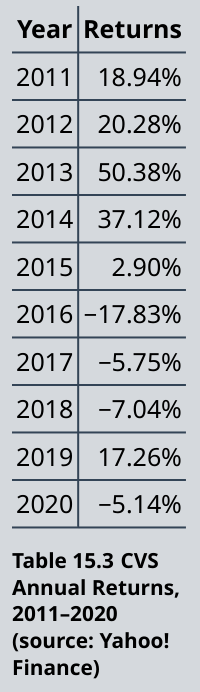
\includegraphics[width=0.4\linewidth]{gfx/m3l1_dahlquist_table15-3_cvs_annual_returns.png}
\par\smallskip{\small \textbf{Bảng 15.3:} Lợi suất hàng năm của CVS, 2011--2020 (nguồn: Yahoo! Finance)}
\end{figure}

Lợi suất trung bình số học trong thập kỷ đó là bao nhiêu? Lợi suất trung bình hình học trong thập kỷ đó là bao nhiêu?

\textbf{Lời giải:}

Xem Bảng 15.4 cho phép tính trung bình số học và trung bình hình học.

\begin{figure}[H]
\centering
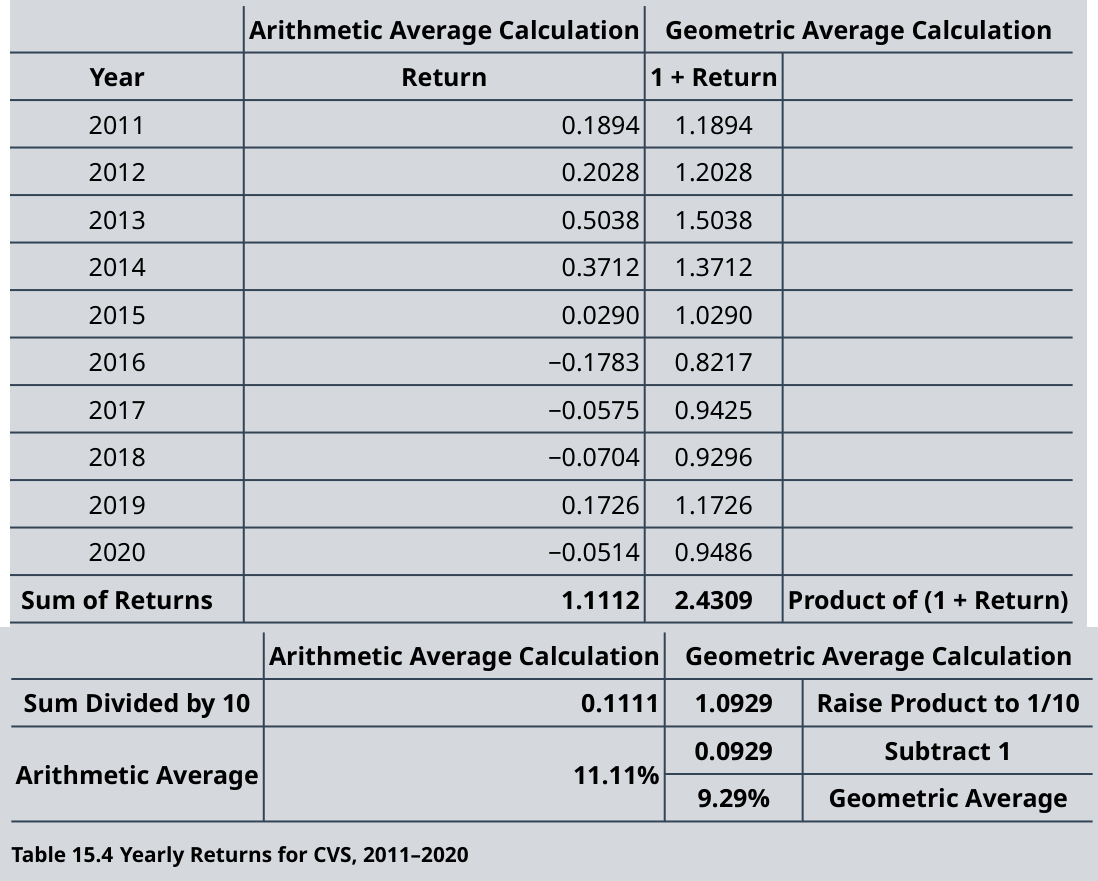
\includegraphics[width=0.85\linewidth]{gfx/m3l1_dahlquist_table15-4_cvs_avg_return_calc.png}
\par\smallskip{\small \textbf{Bảng 15.4:} Lợi suất hàng năm của CVS, 2011--2020}
\end{figure}

Lợi suất trung bình số học của CVS là 11.11\%, và lợi suất trung bình hình học là 9.29\%.
\end{framed}

Cả lợi suất trung bình số học và lợi suất trung bình hình học đều là các phép tính "đúng". Chúng chỉ trả lời các câu hỏi khác nhau. Trung bình hình học cho bạn biết thực tế bạn kiếm được bao nhiêu mỗi năm tính trung bình, theo lãi kép hàng năm. Nó hữu ích để tính mức tăng trưởng của một khoản đầu tư cụ thể qua thời gian. Trung bình số học cho bạn biết bạn kiếm được bao nhiêu trong một năm điển hình. Khi xem xét mô tả lịch sử của phân phối lợi suất và muốn dự đoán những gì nên kỳ vọng trong một năm cụ thể, trung bình số học là phép tính liên quan.

\subsection*{Đo lường Rủi ro}

Mặc dù lợi suất trung bình số học của Delta Airlines (DAL) giai đoạn 2011--2020 là 22.4\%, không có năm nào lợi suất đúng bằng 22.4\%. Thực tế, một số năm lợi suất cao hơn nhiều so với trung bình, chẳng hạn năm 2013, khi lợi suất là 132.61\%. Những năm khác, lợi suất âm, chẳng hạn năm 2011, khi lợi suất là $-35.79\%$. Nhìn vào lợi suất hàng năm trong Bảng 15.2, lợi suất của DAL biến động rất nhiều qua từng năm. Trong tài chính, độ biến động lợi suất này được coi là rủi ro.

\subsection*{Độ Biến động của Lợi suất}

Thước đo phổ biến nhất về độ biến động lợi suất trong tài chính là độ lệch chuẩn (standard deviation) của lợi suất. Độ lệch chuẩn của lợi suất DAL cho giai đoạn mẫu 2011--2020 là 51.9\%. Hãy nhớ rằng nếu phân phối chuẩn (đường cong hình chuông) mô tả lợi suất, thì 68\% (hay khoảng hai phần ba) thời gian, lợi suất trong một năm cụ thể sẽ nằm trong khoảng một độ lệch chuẩn phía trên và một độ lệch chuẩn phía dưới lợi suất trung bình số học. Với lợi suất trung bình 22.4\% của DAL, lợi suất thực tế hàng năm sẽ nằm đâu đó giữa $-29.5\%$ và $74.29\%$ trong hai trên ba năm. Một lợi suất rất cao trên 74.29\% sẽ xảy ra 16\% thời gian; một khoản lỗ rất lớn hơn 29.5\% cũng sẽ xảy ra 16\% thời gian.

Như bạn thấy, có một phạm vi rộng những gì có thể coi là một năm "điển hình" đối với DAL. Mặc dù ta có thể tính lợi suất trung bình, lợi suất trong bất kỳ năm cụ thể nào có khả năng khác với mức trung bình đó. Độ lệch chuẩn càng lớn, phạm vi lợi suất này càng lớn. Do đó, độ lệch chuẩn lớn hơn cho thấy độ biến động lợi suất lớn hơn và do đó rủi ro cao hơn.

\begin{framed}
\textbf{THỰC HÀNH: Tính Độ lệch chuẩn của Lợi suất}

Bạn đã tính lợi suất trung bình số học của CVS là 11.11\% cho giai đoạn 10 năm 2011--2020. Hãy tính độ lệch chuẩn của lợi suất CVS cho cùng giai đoạn (xem Bảng 15.5). Điều này cho bạn biết gì về những gì một nhà đầu tư vào CVS đã trải qua trong một năm điển hình của thập kỷ đó?

\textbf{Lời giải:}

\begin{figure}[H]
\centering
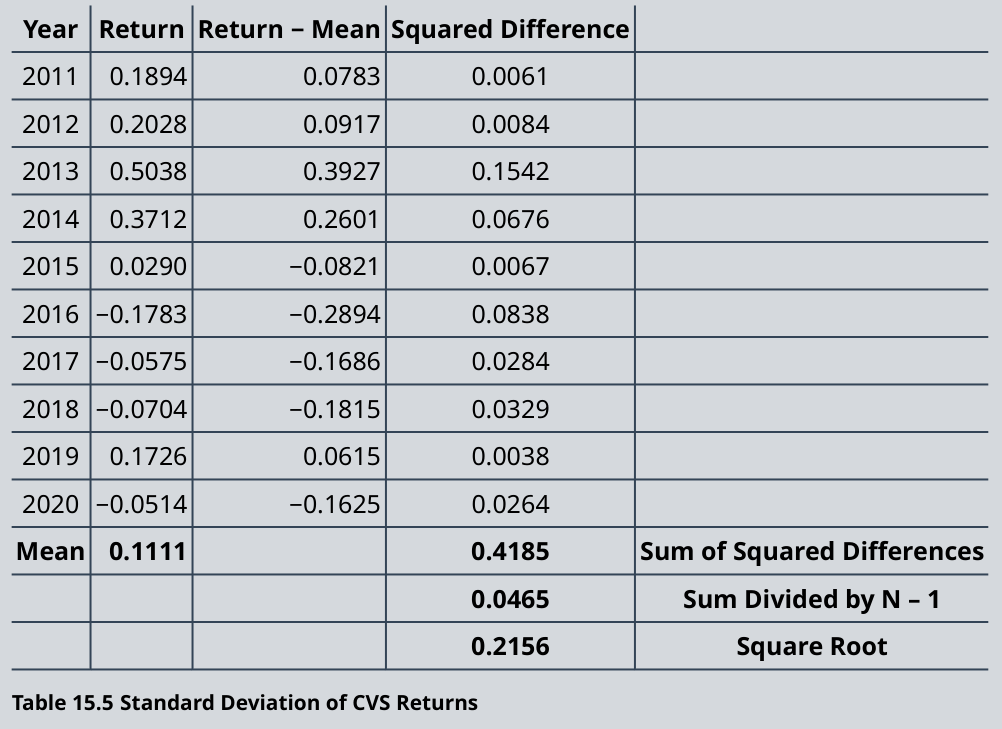
\includegraphics[width=0.55\linewidth]{gfx/m3l1_dahlquist_table15-5_cvs_stddev.png}
\par\smallskip{\small \textbf{Bảng 15.5:} Độ lệch chuẩn của Lợi suất CVS}
\end{figure}

Độ lệch chuẩn của lợi suất CVS trong giai đoạn mẫu 2011--2020 là 21.56\%. Với lợi suất trung bình số học 11.11\%, lợi suất sẽ nằm trong khoảng $-10.45\%$ và $32.67\%$ trong khoảng hai trên ba năm. Mặc dù lợi suất trung bình là 11.11\%, lợi suất trong một năm cụ thể có thể cao hơn hoặc thấp hơn nhiều so với mức trung bình đó. Thực tế, một khoản lỗ hơn 10.45\% được kỳ vọng xảy ra khoảng một lần mỗi sáu năm. Ngoài ra, khoảng một lần mỗi sáu năm, lợi suất lớn hơn 32.67\% cũng được kỳ vọng xảy ra.
\end{framed}

\subsection*{Rủi ro Đặc thù Doanh nghiệp}

Nhà đầu tư mua cổ phiếu với hy vọng cổ phiếu sẽ tăng giá trị và họ sẽ nhận lợi suất dương. Tuy nhiên, bạn có thể thấy rằng ngay cả với các công ty đã ổn định như ExxonMobil và CVS, lợi suất vẫn rất biến động. Nhà đầu tư không bao giờ có thể dự đoán hoàn hảo lợi suất của một cổ phiếu sẽ là bao nhiêu, hay thậm chí liệu nó có dương hay không.

Lợi suất hàng năm của bốn công ty — Delta Airlines (DAL), Southwest Airlines (LUV), ExxonMobil (XOM), và CVS Health Corp. (CVS) — được trình bày trong Bảng 15.6. Mỗi cổ phiếu này đều có những năm hiệu suất tốt hơn hoặc tệ hơn nhiều so với trung bình số học. Thực tế, không cổ phiếu nào có vẻ có một mức lợi suất "điển hình" lặp lại năm này qua năm khác.

\begin{figure}[H]
\centering
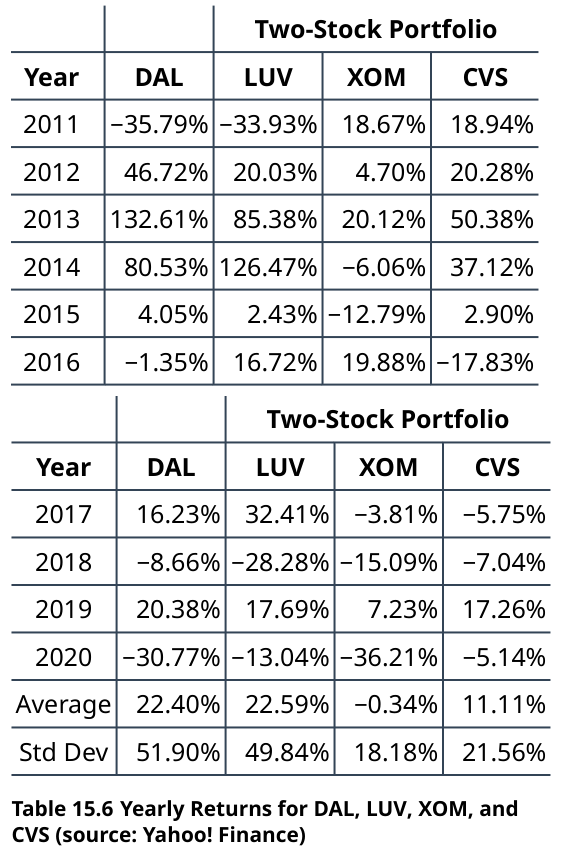
\includegraphics[width=0.75\linewidth]{gfx/m3l1_dahlquist_table15-6_yearly_returns.png}
\par\smallskip{\small \textbf{Bảng 15.6:} Lợi suất hàng năm của DAL, LUV, XOM và CVS (nguồn: Yahoo! Finance)}
\end{figure}

Hình 15.2 trình bày đồ thị lợi suất của từng cổ phiếu trong bốn cổ phiếu này theo năm. Trong đồ thị này, có thể dễ dàng thấy rằng DAL và LUV đều có độ biến động cao hơn, tức lợi suất biến thiên nhiều hơn qua từng năm, so với XOM hoặc CVS. Độ biến động cao hơn này khiến DAL và LUV có độ lệch chuẩn lợi suất cao hơn XOM hoặc CVS.

\begin{figure}[H]
\centering
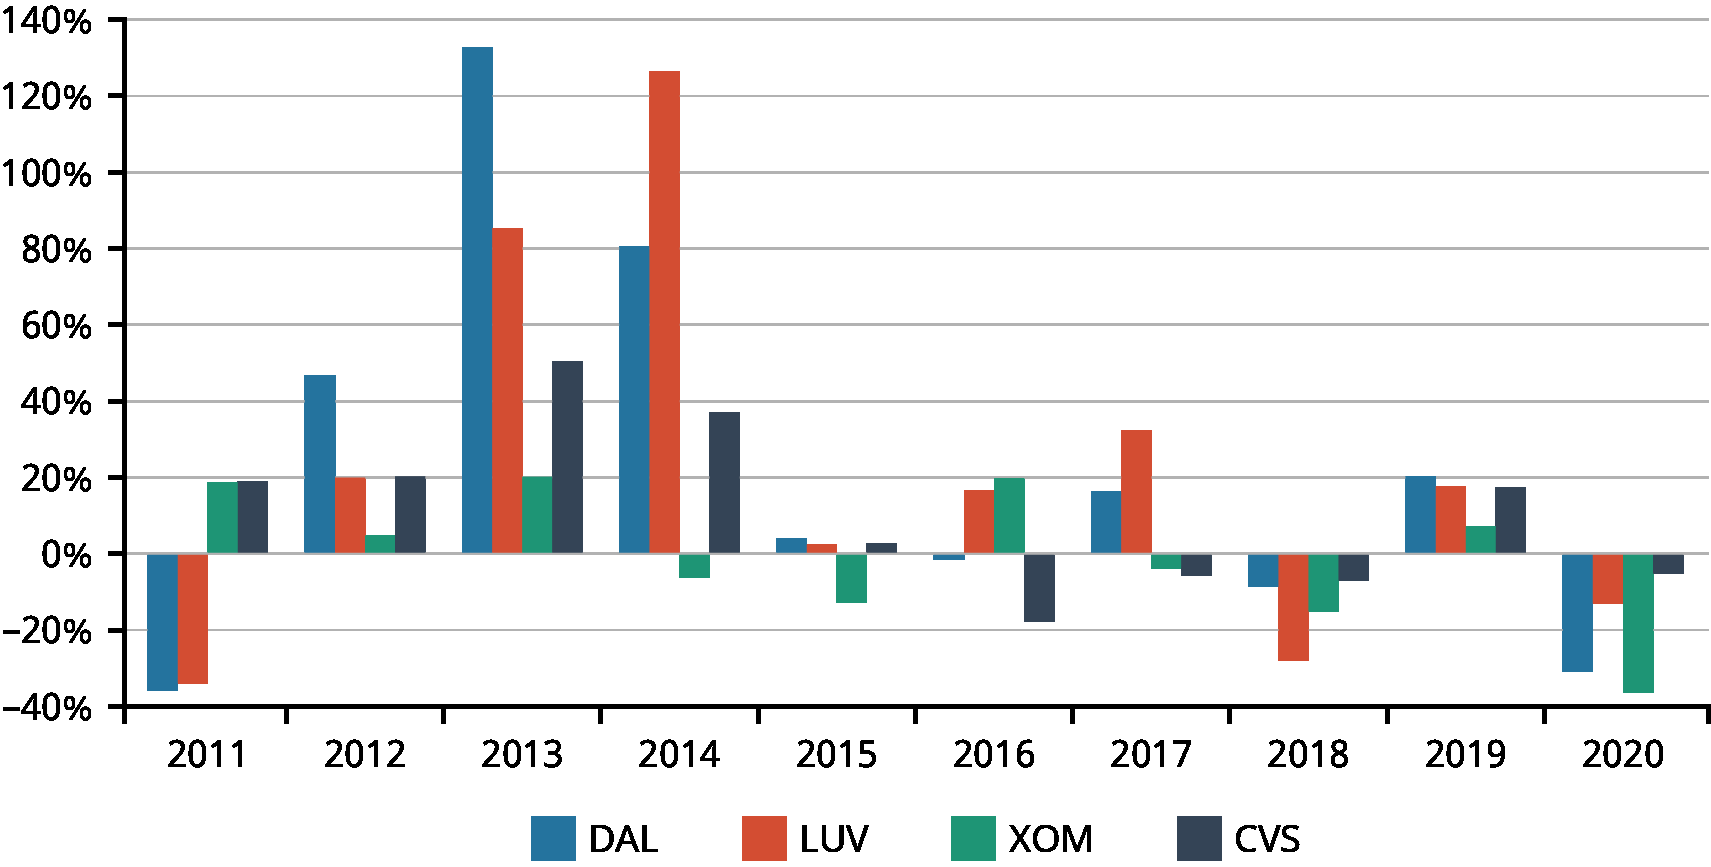
\includegraphics[width=\linewidth,height=0.6\textheight,keepaspectratio]{gfx/m3l1_dahlquist_fig15-2_yearly_returns.png}
\par\smallskip{\small \textbf{Hình 15.2:} Lợi suất hàng năm của DAL, LUV, XOM và CVS (nguồn dữ liệu: Yahoo! Finance)}
\end{figure}

Độ lệch chuẩn được coi là một thước đo rủi ro khi sở hữu một cổ phiếu. Độ lệch chuẩn lợi suất hàng năm của cổ phiếu càng lớn, lợi suất của cổ phiếu đó trong bất kỳ năm nào càng có khả năng lệch xa khỏi mức trung bình. Nói cách khác, lợi suất của cổ phiếu rất khó dự đoán. Mặc dù lợi suất của CVS biến thiên qua từng năm, nó không biến động mạnh như lợi suất của DAL hay LUV.

Tại sao lợi suất cổ phiếu lại biến động nhiều đến vậy? Giá trị cổ phiếu của một công ty thay đổi khi kỳ vọng về doanh thu và chi phí tương lai của công ty thay đổi. Những kỳ vọng này có thể thay đổi do nhiều sự kiện và thông tin mới. Tin tốt về một công ty thường dẫn đến giá cổ phiếu tăng. Ví dụ, DAL thông báo sẽ mở các tuyến bay mới và bay đến các thành phố trước đây chưa phục vụ cho thấy DAL sẽ có nhiều khách hàng hơn và doanh thu nhiều hơn trong tương lai. Hoặc nếu CVS thông báo đã đàm phán được giá thuê thấp hơn cho nhiều địa điểm của mình, nhà đầu tư sẽ kỳ vọng chi phí công ty giảm, dẫn đến lợi nhuận cao hơn. Những loại thông báo này thường đi kèm với giá cổ phiếu cao hơn. Ngược lại, nếu phi công và tiếp viên của DAL đàm phán được mức lương cao hơn, chi phí của DAL sẽ tăng, gây áp lực giảm lên lợi nhuận và giá cổ phiếu.

\begin{framed}
\textbf{LIÊN KẾT ĐẾN VIỆC HỌC: Peloton và Rủi ro}

Một ví dụ về cách tin tức có thể ảnh hưởng đến giá cổ phiếu xảy ra vào ngày 5/5/2021, khi Peloton thu hồi toàn bộ sản phẩm Tread+ và Tread sau cái chết thương tâm của một trẻ em và 70 ca chấn thương liên quan đến việc sử dụng sản phẩm. Ngày hôm trước, cổ phiếu Peloton giao dịch ở mức \$96.70/cổ phiếu. Giá cổ phiếu giảm khoảng 15\% khi việc thu hồi được công bố. Giá đóng cửa của cổ phiếu Peloton ngày 5/5 là \$82.62.
\end{framed}

\section{15.2 Rủi ro và Lợi suất của Nhiều Tài sản}

\subsection*{Mục tiêu học tập}
Sau khi hoàn thành mục này, bạn sẽ có thể:
\begin{itemize}
  \item Giải thích lợi ích của đa dạng hóa (diversification).
  \item Mô tả mối quan hệ giữa rủi ro và lợi suất đối với các danh mục đầu tư lớn.
  \item So sánh rủi ro đặc thù doanh nghiệp và rủi ro hệ thống.
  \item Thảo luận cách quy mô danh mục đầu tư ảnh hưởng đến rủi ro.
\end{itemize}

\subsection*{Đa dạng hóa}

Đến nay, chúng ta đã xem xét lợi suất và độ biến động của một cổ phiếu riêng lẻ. Tuy nhiên, hầu hết nhà đầu tư sở hữu cổ phiếu của nhiều công ty. Tập hợp cổ phiếu này được gọi là danh mục đầu tư (portfolio). Hãy cùng khám phá vì sao nhà đầu tư nên nắm giữ một danh mục cổ phiếu thay vì chỉ chọn một cổ phiếu yêu thích duy nhất để sở hữu.

Chúng ta đã thấy rằng nhà đầu tư sở hữu DAL có lợi suất trung bình hàng năm 20.87\% nhưng cũng có độ lệch chuẩn lớn 51.16\%. Nhà đầu tư dùng toàn bộ vốn để mua cổ phiếu DAL đã có kết quả cực kỳ tốt trong giai đoạn 2012--2014. Nhưng vào năm 2020, các nhà đầu tư đó đã mất gần một phần ba số tiền khi COVID-19 khiến việc đi lại bằng đường hàng không toàn cầu giảm mạnh. Để bảo vệ trước các kết quả cực đoan này, nhà đầu tư thực hành cái gọi là đa dạng hóa, tức nắm giữ nhiều loại cổ phiếu khác nhau trong danh mục đầu tư của mình.

Giả sử, ví dụ, bạn đã tiết kiệm được \$50,000 muốn đầu tư. Nếu bạn mua \$50,000 cổ phiếu DAL, bạn sẽ không được đa dạng hóa. Lợi suất của bạn sẽ chỉ phụ thuộc vào lợi suất của cổ phiếu DAL. Nếu thay vào đó, bạn dùng \$5,000 để mua cổ phiếu DAL và dùng \$45,000 còn lại để mua chín cổ phiếu khác, bạn đang đa dạng hóa. Lợi suất của bạn sẽ phụ thuộc không chỉ vào lợi suất của DAL mà còn vào lợi suất của chín cổ phiếu khác trong danh mục. Nhà đầu tư thực hành đa dạng hóa để quản lý rủi ro.

Điều này tương tự câu nói "Đừng bỏ hết trứng vào một giỏ." Nếu bạn để tất cả trứng vào một giỏ và giỏ đó vỡ, tất cả trứng của bạn sẽ rơi và vỡ. Nếu bạn phân tán trứng ra nhiều giỏ, khó có khả năng tất cả các giỏ đều vỡ và tất cả trứng đều bể. Một giỏ có thể vỡ, và bạn sẽ mất số trứng trong giỏ đó, nhưng bạn vẫn còn những giỏ trứng khác. Ý tưởng tương tự cũng đúng với đầu tư. Nếu bạn sở hữu cổ phiếu của một công ty làm ăn kém, thậm chí phá sản, bạn sẽ mất số tiền đã đặt vào khoản đầu tư cụ thể đó. Tuy nhiên, với một danh mục đa dạng hóa, bạn không mất toàn bộ số tiền vì tiền của bạn được phân tán qua nhiều công ty khác nhau.

\begin{framed}
\textbf{LIÊN KẾT ĐẾN VIỆC HỌC: Đa dạng hóa}

Fidelity Investments Inc. là một công ty dịch vụ tài chính đa quốc gia và là một trong những công ty quản lý tài sản lớn nhất thế giới. Trong video giáo dục dành cho nhà đầu tư này, Fidelity giải thích đa dạng hóa là gì và nó ảnh hưởng thế nào đến danh mục đầu tư của nhà đầu tư.
\end{framed}

Bảng 15.7 trình bày lợi suất của nhà đầu tư đặt 50\% tiền vào DAL và 50\% còn lại vào LUV, XOM, hoặc CVS. Lưu ý rằng độ lệch chuẩn lợi suất thấp hơn đối với các danh mục hai cổ phiếu so với DAL là một khoản đầu tư riêng lẻ.

\begin{figure}[H]
\centering
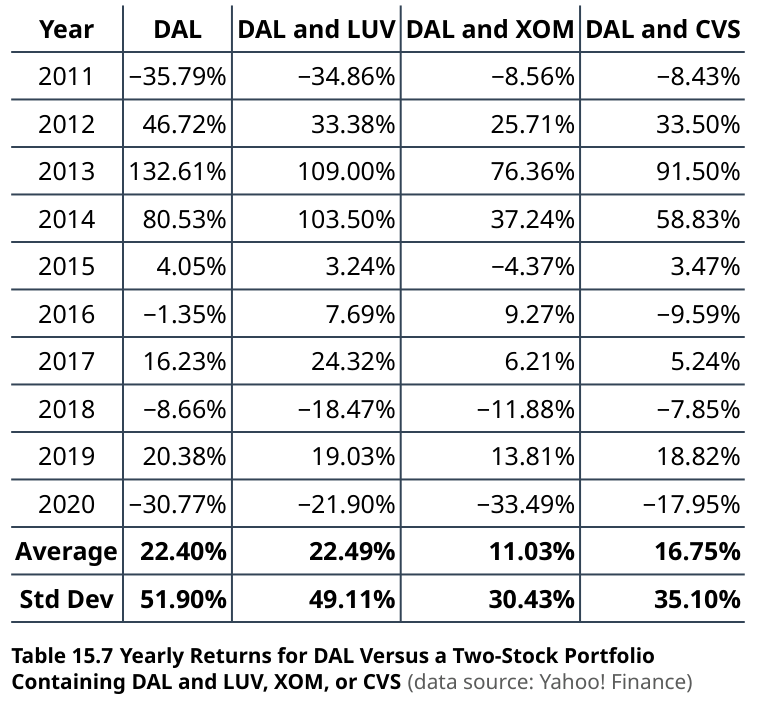
\includegraphics[width=0.85\linewidth]{gfx/m3l1_dahlquist_table15-7_two_stock_portfolio_returns.png}
\par\smallskip{\small \textbf{Bảng 15.7:} Lợi suất hàng năm của DAL so với Danh mục Hai Cổ phiếu gồm DAL và LUV, XOM, hoặc CVS (nguồn dữ liệu: Yahoo! Finance)}
\end{figure}

Khi nhà đầu tư đa dạng hóa danh mục của mình, độ biến động của một cổ phiếu cụ thể trở nên kém quan trọng hơn. XOM có những năm tốt với lợi suất trên trung bình và những năm xấu với lợi suất dưới trung bình (thậm chí âm), giống như DAL. Nhưng những năm mà các lợi suất trên/dưới trung bình đó xảy ra không phải lúc nào cũng giống nhau giữa hai công ty. Ví dụ, năm 2014, lợi suất của DAL lớn hơn 80\%, trong khi lợi suất của XOM âm. Mặt khác, năm 2011, khi DAL có lợi suất $-35.15\%$, XOM lại có lợi suất dương. Khi nắm giữ nhiều hơn một cổ phiếu, lãi ở một cổ phiếu có thể bù đắp lỗ ở cổ phiếu khác, làm giảm bớt một phần độ biến động.

Khi nhà đầu tư chỉ nắm giữ một cổ phiếu, độ biến động của cổ phiếu đó đóng góp 100\% vào độ biến động của danh mục. Khi nắm giữ hai cổ phiếu, độ biến động của mỗi cổ phiếu đóng góp vào độ biến động của danh mục. Tuy nhiên, độ biến động của danh mục không đơn giản là trung bình độ biến động của từng cổ phiếu nắm giữ độc lập. Mức độ tương quan giữa hai cổ phiếu, hay chúng di chuyển cùng nhau đến đâu, sẽ ảnh hưởng đến độ biến động của danh mục.

Bạn sẽ nhớ lại từ nghiên cứu về tương quan trong Phân tích Hồi quy trong Tài chính rằng hệ số tương quan mô tả cách hai biến di chuyển tương đối với nhau. Hệ số tương quan bằng 1 nghĩa là có tương quan dương hoàn hảo giữa hai biến, trong khi hệ số tương quan bằng $-1$ nghĩa là hai biến di chuyển hoàn toàn ngược nhau. Các cổ phiếu cùng ngành thường có xu hướng tương quan mạnh hơn các cổ phiếu ở các ngành rất khác nhau. Trong giai đoạn 2011--2020, hệ số tương quan giữa DAL và LUV là 0.87, hệ số tương quan giữa DAL và XOM là 0.35, và hệ số tương quan giữa DAL và CVS là 0.79. Kết hợp các cổ phiếu không tương quan dương hoàn hảo trong một danh mục sẽ giảm rủi ro.

Lưu ý rằng nhà đầu tư sở hữu DAL và LUV từ 2011 đến 2020 sẽ có độ lệch chuẩn danh mục thấp hơn, nhưng không thấp hơn nhiều, so với nhà đầu tư chỉ sở hữu DAL. Vì hệ số tương quan nhỏ hơn 1, độ lệch chuẩn giảm xuống. Tuy nhiên, vì hai cổ phiếu cùng ngành và chịu ảnh hưởng bởi nhiều vấn đề kinh tế giống nhau, hệ số tương quan tương đối cao, và việc kết hợp hai cổ phiếu này chỉ giảm rủi ro một phần nhỏ.

Điều này là vì, là các hãng hàng không, DAL và LUV đối mặt với nhiều điều kiện thị trường giống nhau. Trong những năm kinh tế mạnh, thời tiết tốt, giá nhiên liệu thấp, và người dân đi lại nhiều, cả hai công ty đều làm ăn tốt. Khi điều gì đó như thời tiết xấu làm giảm lượng di chuyển hàng không trong nhiều tuần, cả hai công ty đều bị ảnh hưởng. Bằng cách nắm giữ LUV bên cạnh DAL, nhà đầu tư có thể giảm phơi nhiễm với rủi ro đặc thù của DAL (có thể là vấn đề với hệ thống đặt vé của DAL), nhưng họ không giảm được phơi nhiễm với rủi ro liên quan đến ngành hàng không (có thể là giá nhiên liệu máy bay tăng). DAL và LUV có xu hướng có lợi suất dương trong cùng những năm và lợi suất âm trong cùng những năm.

Mặt khác, nhà đầu tư thêm XOM vào danh mục của họ thấy độ lệch chuẩn thấp hơn đáng kể so với những người chỉ nắm giữ DAL. Trong những năm giá nhiên liệu máy bay tăng, gây hại cho lợi nhuận của cả DAL và LUV, XOM có khả năng có lợi nhuận cao. Đa dạng hóa danh mục qua các công ty ít tương quan hơn sẽ giảm độ lệch chuẩn của danh mục nhiều hơn.

\begin{framed}
\textbf{LIÊN KẾT ĐẾN VIỆC HỌC: Cách Xây dựng một Danh mục Đa dạng hóa}

Nhân vật truyền hình, cựu quản lý quỹ phòng hộ, và tác giả Jim Cramer khuyến khích nhà đầu tư xây dựng một danh mục đa dạng hóa, không quá 20\% danh mục trong một ngành. Ông đề xuất nhà đầu tư có thể xây dựng danh mục đa dạng hóa bằng cách mua từ năm đến mười cổ phiếu.
\end{framed}

\subsection*{Quy mô Danh mục và Rủi ro}

Khi bạn thêm nhiều cổ phiếu vào danh mục, độ biến động, hay độ lệch chuẩn, của danh mục giảm xuống. Độ biến động của từng tài sản riêng lẻ trở nên ngày càng kém quan trọng. Như đã thảo luận trước đó, rủi ro liên quan đến các sự kiện của một công ty cụ thể được gọi là rủi ro đặc thù doanh nghiệp, hay rủi ro phi hệ thống (unsystematic risk). Ví dụ về rủi ro phi hệ thống bao gồm một công ty đối mặt với vụ kiện trách nhiệm sản phẩm, một công ty phát minh sản phẩm mới, hoặc phát hiện gian lận kế toán. Nắm giữ một danh mục cổ phiếu nghĩa là nếu một công ty bạn đầu tư phá sản do quản lý kém, bạn không mất toàn bộ tiền tiết kiệm vì một phần tiền của bạn được đầu tư vào các công ty khác. Đa dạng hóa danh mục bảo vệ bạn khỏi bị ảnh hưởng đáng kể bởi rủi ro phi hệ thống.

Tuy nhiên, có một mức mà rủi ro danh mục không giảm xuống dưới đó, dù danh mục có đa dạng hóa đến đâu. Rủi ro không bao giờ biến mất này được gọi là rủi ro hệ thống (systematic risk). Rủi ro hệ thống là rủi ro của việc nắm giữ danh mục thị trường.

Chúng ta đã nói về lý do lợi suất của một công ty có thể biến động; ví dụ, việc công ty phát hiện một công nghệ mới hoặc bị kiện trách nhiệm sản phẩm sẽ ảnh hưởng đặc thù đến công ty đó. Cũng có những sự kiện ảnh hưởng rộng rãi đến toàn thị trường chứng khoán. Thay đổi trong chính sách tiền tệ và lãi suất của Cục Dự trữ Liên bang ảnh hưởng đến tất cả các công ty. Các sự kiện địa chính trị, bão lớn, và đại dịch cũng có thể ảnh hưởng đến toàn bộ thị trường. Nhà đầu tư cổ phiếu không thể tránh khỏi loại rủi ro này. Rủi ro không thể tránh khỏi này chính là rủi ro hệ thống mà nhà đầu tư cổ phiếu phải gánh chịu. Rủi ro hệ thống này không thể loại bỏ thông qua đa dạng hóa.

Ngoài ra, theo nghiên cứu của Meir Statman, độ lệch chuẩn của một danh mục giảm nhanh khi số lượng cổ phiếu trong danh mục tăng từ một lên hai hoặc ba. Tăng quy mô danh mục giúp giảm độ lệch chuẩn, và do đó giảm rủi ro, của danh mục. Tuy nhiên, khi danh mục tăng quy mô, mức rủi ro giảm được khi thêm một cổ phiếu nữa vào danh mục sẽ giảm dần. Một nhà đầu tư cần bao nhiêu cổ phiếu để danh mục được đa dạng hóa tốt? Không có con số chính xác mà tất cả các nhà quản lý tài chính đều đồng ý. Một danh mục gồm 15 cổ phiếu tương quan cao sẽ mang lại ít lợi ích đa dạng hóa hơn một danh mục gồm 10 cổ phiếu có hệ số tương quan thấp hơn. Một danh mục gồm American Airlines, Spirit Airlines, United Airlines, Southwest Airlines, Delta Airlines, và Jet Blue, cùng một vài cổ phiếu khác, không được đa dạng hóa tốt vì tập trung nặng vào ngành hàng không. Thuật ngữ danh mục đa dạng hóa là một khái niệm tương đối, nhưng nhà đầu tư bình thường có thể tạo một danh mục đa dạng hóa hợp lý với khoảng một tá cổ phiếu.


% ---- Lesson 2: Efficient Frontier, Sharpe Ratio and Downside Risk Metrics ----
% Thứ tự đọc: Lesson Notes -> Đọc thêm
\chapter{Đường Biên Hiệu quả, Tỷ số Sharpe và Các Thước đo Rủi ro Sụt giảm}
\label{ch:M3L2}

% Lesson: Efficient Frontier, Sharpe Ratio and Downside Risk Metrics

\section*{Lesson Notes}

MODULE 3 | BÀI 2

{\small
\begin{longtable}{>{\raggedright\arraybackslash}p{0.213\linewidth}>{\raggedright\arraybackslash}p{0.727\linewidth}}
\toprule
\textbf{Thời gian đọc} & 6 giờ \\
\addlinespace[2pt]
\textbf{Kiến thức nền tảng} & Lợi suất phần trăm-log, các thước đo rủi ro, phân phối chuẩn và phân phối t \\
\addlinespace[2pt]
\textbf{Từ khóa} & Điều chỉnh cổ tức, giá đóng cửa điều chỉnh, chia tách cổ phiếu, lợi suất, Value at Risk, có điều kiện, kỳ vọng \\
\addlinespace[2pt]
\bottomrule
\end{longtable}
}

\emph{Trong bài học này, chúng ta tiếp tục khám phá một số loại lợi suất quan trọng. Cụ thể, chúng ta giới thiệu tổng lợi suất, lợi suất điều chỉnh cổ tức, và lợi suất vượt trội. Chúng ta thảo luận về giá đóng cửa điều chỉnh và hướng dẫn cách tính nó. Sau đó, chúng ta tiến đến Tỷ số Sharpe, một thước đo nền tảng trong lý thuyết danh mục đầu tư hiện đại, đo lường hiệu suất đã điều chỉnh theo rủi ro. Tỷ số này giúp nhà đầu tư và nhà phân tích đánh giá lợi suất của một khoản đầu tư trong mối quan hệ với rủi ro của nó. Cuối cùng, chúng ta giới thiệu Value at Risk (VaR), một thước đo rủi ro then chốt được sử dụng rộng rãi trong ngành tài chính. Chúng ta sẽ đề cập đến nhiều phương pháp tính VaR, bao gồm phương pháp lịch sử, tham số (sử dụng cả phân phối chuẩn và phân phối t), và mô phỏng Monte Carlo. Chúng ta cũng giới thiệu khái niệm Conditional Value at Risk (CVaR), cung cấp thêm hiểu biết về rủi ro đuôi (tail risk).}

\begin{lstlisting}[language=Python,escapeinside={(*@}{@*)}]
import pandas as pd
import numpy as np
import matplotlib.pyplot as plt
import seaborn as sns
import fredapi as fa
from scipy import stats
import numpy as np
sns.set()
\end{lstlisting}

\begin{lstlisting}[language=Python,escapeinside={(*@}{@*)}]
assets = ['MSFT', 'AAPL', 'AMZN', 'TSLA', 'GOOGL'] # (*@Các@*) (*@tài@*) (*@sản@*) (*@trong@*) (*@danh@*) (*@mục@*)

# (*@Tải@*) (*@giá@*) (*@tài@*) (*@sản@*)
asset_prices = pd.read_csv("portfolio_prices.csv", index_col = "Date", parse_dates = True)

# (*@Tải@*) (*@dữ@*) (*@liệu@*) (*@lãi@*) (*@suất@*) (*@phi@*) (*@rủi@*) (*@ro@*) ((*@Tín@*) (*@phiếu@*) (*@Kho@*) (*@bạc@*) 3 (*@tháng@*))
risk_free = pd.read_csv("risk_free.csv", index_col = "Date", parse_dates = True)


r = asset_prices.pct_change().dropna() # (*@Tính@*) (*@lợi@*) (*@suất@*) (*@phần@*) (*@trăm@*) (*@hàng@*) (*@ngày@*)
\end{lstlisting}

\section{Tổng Lợi suất và Lợi suất Điều chỉnh Cổ tức}

Trong bài học trước, chúng ta đã thảo luận về lợi suất danh mục đầu tư và phương sai. Chúng ta đã học cụ thể cách tính lợi suất và chuẩn hóa chúng theo năm, cùng một số đặc điểm riêng của hai loại lợi suất chính: phần trăm và logarit.

Trong bài học này, chúng ta bắt đầu bằng việc mở rộng sang \textbf{tổng lợi suất, lợi suất điều chỉnh cổ tức, và lợi suất vượt trội} như một điều kiện tiên quyết cho nhiều loại tỷ số mà một kỹ sư dữ liệu tài chính cần nắm được. Trong quá trình đó, khái niệm \emph{giá đóng cửa điều chỉnh} sẽ tự nhiên xuất hiện.

\subsection{Tổng Lợi suất và Lợi suất Điều chỉnh Cổ tức}

Tổng lợi suất đại diện cho mức lãi hoặc lỗ tổng thể trên một khoản đầu tư trong một giai đoạn cụ thể. Nó tính đến mọi hình thức thu nhập:

$$
\text{Tổng Lợi suất} = \frac{(p_{T} - p_{0}) + (D + I)}{p_{0}}
$$

Trong đó:
\begin{itemize}
  \item $T$: Cuối giai đoạn.
  \item $D$: Cổ tức.
  \item $I$: Bất kỳ hình thức thu nhập bổ sung nào khoản đầu tư cụ thể mang lại.
\end{itemize}

Lợi suất điều chỉnh cổ tức tương tự tổng lợi suất, ngoại trừ chỉ tính đến cổ tức đã trả:

$$
\text{Lợi suất Điều chỉnh Cổ tức} = \frac{(p_{T} - p_{0}) + D}{p_{0}}
$$

Hai công thức trên khá dễ hiểu và trực quan, nhưng để đi sâu hơn một chút, chúng ta cần tính chúng với một giá đóng cửa và cổ tức trên mỗi cổ phiếu cho trước.

Hãy xem xét một cổ phiếu X với giá đóng cửa và cổ tức sau đây trong ba năm (tất cả giá đều tính tại ngày giao dịch không hưởng quyền, ex-date):

\begin{center}
\begin{tabular}{lrr}
\toprule
Năm & Giá (\$) & Cổ tức (\$) \\
\midrule
2019: & 105 & 2 \\
2020: & 112 & 2.2 \\
2021: & 118 & 2.4 \\
2022: & 116 & 2.3 \\
\bottomrule
\end{tabular}
\end{center}

Lợi suất điều chỉnh cổ tức cho giai đoạn 2021 đến 2022 là:

$$
r^{\text{Adj}}_{2021 - 2022} = \frac{116 - 118 + 2.3}{118} = 0.0025
$$

trong khi lợi suất không điều chỉnh là:

$$
r_{2021 - 2022} = \frac{116 - 118}{118} = -0.017
$$

Mặc dù hai lợi suất khá gần nhau, dấu của chúng lại khác nhau! Và vì mọi nhà đầu tư nắm giữ cổ phiếu đều nhận được cổ tức, chúng ta cần tính đến điều này khi tính lợi suất. Điều đó dẫn ta đến giá đóng cửa điều chỉnh như một phép biến đổi giá tiện lợi có tính đến cổ tức (cùng với chia tách cổ phiếu và các hành động doanh nghiệp khác).

\subsection{Giá Đóng cửa Điều chỉnh}

Khi tải dữ liệu cổ phiếu, bạn sẽ thấy cả giá "close" và "adjusted close". Nhiều nhà phân tích mặc định dùng giá đóng cửa điều chỉnh, nhưng đây không phải là lựa chọn nên thực hiện mà không hiểu rõ khái niệm đằng sau Giá Đóng cửa Điều chỉnh.

\textbf{Khái niệm chính:} Giá đóng cửa điều chỉnh là một \textbf{giá lý thuyết} kết hợp cổ tức và chia tách như thể bạn đã tái đầu tư toàn bộ. Đây không phải là một mức giá từng thực sự tồn tại trên thị trường.

\textbf{Ba sự thật quan trọng:}

\begin{enumerate}
  \item \textbf{Giả định Tái đầu tư}: Coi cổ tức như thể được tự động tái đầu tư thành thêm cổ phiếu
  \item \textbf{Thay đổi Hồi tố}: Giá lịch sử thay đổi khi có cổ tức/chia tách mới xảy ra
  \item \textbf{Lý thuyết, không phải Thực tế}: Giá cổ phiếu không phải lúc nào cũng điều chỉnh chính xác như lý thuyết dự đoán
\end{enumerate}

\textbf{Tại sao nên dùng?}
\begin{itemize}
  \item Các phép tính lợi suất hoạt động chính xác qua các đợt chia tách
  \item Các thước đo độ biến động phản ánh mọi nguồn lợi suất
  \item Kiểm định lùi (backtesting) không bị gián đoạn tại các sự kiện doanh nghiệp
\end{itemize}

\textbf{Tại sao không nên dùng?}
\begin{itemize}
  \item Không phải giá giao dịch thực tế
  \item Thay đổi theo thời gian (dữ liệu tải hôm nay $\neq$ hôm qua cho cùng một ngày)
  \item Không khớp với lãi/lỗ giao dịch thực tế của bạn
\end{itemize}

Hãy chắc chắn bạn đã đọc phương pháp Yahoo Multipliers để tính Giá Đóng cửa Điều chỉnh từ Giá Đóng cửa, Cổ tức, và Chia tách.

Dưới đây là một ví dụ sử dụng TSLA.

\begin{lstlisting}[language=Python,escapeinside={(*@}{@*)}]
# Figure 1
tsla = pd.read_csv("TSLA_stock_price.csv")
tsla.set_index('date', inplace=True)
tsla.index = pd.to_datetime(tsla.index)

splits = {'2022-08-25' : 3, "2020-08-31" : 5} # (*@Ngày@*) (*@và@*) (*@hệ@*) (*@số@*) (*@nhân@*) (*@của@*) (*@các@*) (*@đợt@*) (*@chia@*) (*@tách@*) TSLA

tsla['Adjusted Close'] = tsla['close'].copy()

for date, split in splits.items():
    date = pd.to_datetime(date) - pd.Timedelta(days=1)
    tsla.loc[:date, 'Adjusted Close'] = tsla.loc[:date, 'Adjusted Close'] / split

tsla[['close', 'Adjusted Close']].loc["2016":].plot(figsize=(12, 8), subplots = True)
plt.show()
\end{lstlisting}

\begin{figure}[H]
\centering
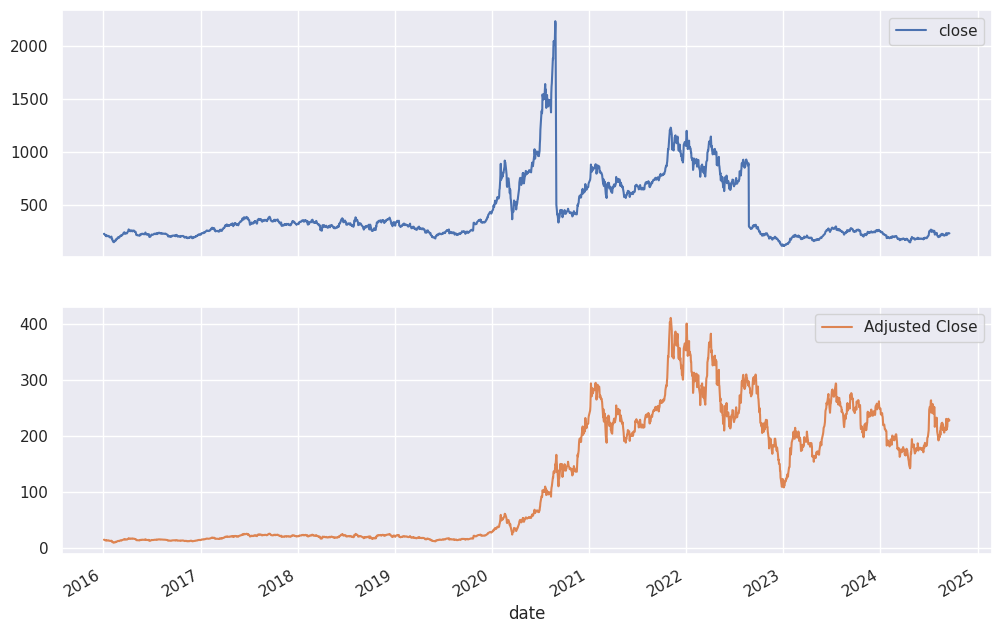
\includegraphics[width=\linewidth,height=0.6\textheight,keepaspectratio]{gfx/m3l2_notes_fig1_tsla_split_adjusted_close.png}
\par\smallskip{\small \textbf{Hình 2.1:} Giá đóng cửa (close) và giá đóng cửa điều chỉnh (adjusted close) của TSLA}
\end{figure}

Trong Hình 2.1, ta có thể thấy sự khác biệt giữa giá đóng cửa và giá đóng cửa điều chỉnh. Ta nhận thấy sự phân kỳ về thang đo (trục $y$), tỷ lệ thuận với các đợt chia tách. Ngoài ra, trong đồ thị giá đóng cửa, ta quan sát thấy mức giảm giá theo phương thẳng đứng vào những ngày diễn ra chia tách. Điều này là dự kiến vì chia tách giữ nguyên vốn hóa thị trường của TSLA, làm giá cổ phiếu giảm tức thì.

\textbf{Bài tập 1}

Tính lợi suất hàng ngày (phần trăm hoặc log) của giá đóng cửa và giá đóng cửa điều chỉnh của TSLA. Chúng có khác nhau không?

\textbf{Bài tập 2}

Tạo tài khoản trên AlphaVantage và lấy một APIKEY. Chọn một tài sản đã trải qua nhiều đợt chia tách (2 lần trở lên) và đã trả một số cổ tức (2 lần trở lên), rồi tải giá đóng cửa (chưa điều chỉnh). Sử dụng phương pháp Yahoo trong đường dẫn ở trên để tính giá đóng cửa điều chỉnh. Vẽ biểu đồ kết quả như Hình 2.1.

\subsection{Lợi suất theo Trọng số Thời gian (Time-Weighted Returns)}

Trong khi giá đóng cửa điều chỉnh cung cấp một cách tiện lợi để tính lợi suất cho các chứng khoán riêng lẻ, quản lý danh mục đầu tư lại đặt ra một độ phức tạp bổ sung: dòng tiền xảy ra tại các thời điểm khác nhau trong suốt giai đoạn đầu tư. Nhà đầu tư có thể nạp thêm vốn hoặc rút tiền tại các thời điểm tùy ý, và các quyết định về thời điểm này, vốn thường nằm ngoài tầm kiểm soát của người quản lý danh mục, có thể làm sai lệch đáng kể các thước đo hiệu suất nếu không được xử lý đúng cách. Phương pháp lợi suất theo trọng số thời gian (time-weighted return, TWR) giải quyết thách thức này bằng cách tách biệt hiệu suất do các quyết định đầu tư của người quản lý tạo ra khỏi ảnh hưởng của các dòng tiền do khách hàng khởi tạo.

Nguyên lý nền tảng của TWR là phân rã toàn bộ giai đoạn đầu tư thành các giai đoạn con được xác định bởi các dòng tiền bên ngoài xảy ra. Trong mỗi giai đoạn con, không có khoản nạp hay rút nào xảy ra, cho phép ta tính một lợi suất theo kỳ nắm giữ đơn giản. Lợi suất theo trọng số thời gian sau đó thu được bằng cách liên kết các lợi suất giai đoạn con này theo cách nhân (hình học). Về mặt hình thức, nếu ta chia khung thời gian đầu tư thành $n$ giai đoạn con, TWR được cho bởi:

$$
\text{TWR} = \left[\prod_{i=1}^{n}(1 + r_i)\right] - 1
$$

trong đó $r_i$ đại diện cho lợi suất của giai đoạn con thứ $i$. Việc tính lợi suất mỗi giai đoạn con đòi hỏi lưu ý cẩn thận đến quy ước thời điểm được dùng cho các dòng tiền. Có hai cách tiếp cận chuẩn trong thực tế, và cần hiểu rõ cả hai.

\textbf{Quy ước 1: Dòng tiền vào Cuối Giai đoạn con}

Khi dòng tiền được ghi nhận vào cuối mỗi giai đoạn con, công thức lợi suất là:

$$
r_i = \frac{V_i - V_{i-1} - CF_i}{V_{i-1}}
$$

trong đó $V_{i-1}$ là giá trị danh mục vào đầu giai đoạn con $i$, $V_i$ là giá trị vào cuối (sau dòng tiền), và $CF_i$ là dòng tiền ròng bên ngoài xảy ra vào cuối giai đoạn con $i$. Theo quy ước này, danh mục sinh lợi trên $V_{i-1}$ trong suốt giai đoạn, và chỉ đến cuối cùng dòng tiền mới xảy ra. Khoản nạp mang dấu dương và khoản rút mang dấu âm.

\textbf{Quy ước 2: Dòng tiền vào Đầu Giai đoạn con}

Ngược lại, khi dòng tiền được ghi nhận vào đầu mỗi giai đoạn con, công thức lợi suất trở thành:

$$
r_i = \frac{V_i - (V_{i-1} + CF_i)}{V_{i-1} + CF_i} = \frac{V_i}{V_{i-1} + CF_i} - 1
$$

trong đó $V_{i-1}$ là giá trị danh mục ngay trước khi dòng tiền xảy ra, $CF_i$ là dòng tiền vào đầu giai đoạn con $i$, và $V_i$ là giá trị vào cuối giai đoạn con. Ở đây, danh mục sinh lợi trên cơ sở vốn đã điều chỉnh $V_{i-1} + CF_i$ trong suốt giai đoạn.

\textbf{Hiểu Sự khác biệt}

Sự khác biệt giữa hai quy ước này không chỉ là vấn đề ký hiệu, nó ảnh hưởng đến cách ta cấu trúc các phép tính. Hãy xem một ví dụ đơn giản: một danh mục bắt đầu ngày với \$100,000, sinh lợi 2\% trong ngày, và sau đó nhận một khoản nạp \$10,000 vào cuối ngày. Theo Quy ước 1 (dòng tiền cuối kỳ), giá trị danh mục trước khoản nạp là \$102,000, khoản nạp đưa nó lên \$112,000, và lợi suất là $(102{,}000 - 100{,}000)/100{,}000 = 2\%$. Theo Quy ước 2, nếu ta biết trước khoản nạp sẽ đến vào đầu kỳ, ta sẽ tính lợi suất trên \$110,000, đạt \$112,200 với lợi suất 2\%, và đo $r = (112{,}200 - 110{,}000)/110{,}000 = 2\%$. Cả hai quy ước cho ra cùng lợi suất khi áp dụng nhất quán, nhưng giả định về thời điểm phải rõ ràng.

Trong thực tế, \textbf{Quy ước 1 (cuối kỳ) phổ biến hơn} vì một số lý do. Thứ nhất, định giá danh mục thường được thực hiện vào lúc đóng cửa giao dịch, và dòng tiền được ghi nhận tại thời điểm đóng cửa đó. Thứ hai, nhiều hệ thống đo lường hiệu suất tự nhiên áp dụng quy ước này vì nó phù hợp với cách giao dịch được thanh toán và cách dữ liệu được đánh dấu thời gian. Thứ ba, khi dòng tiền xảy ra trong ngày, coi chúng là cuối kỳ giúp đơn giản hóa toán học vì ta không cần phân bổ theo tỷ lệ lợi suất cho các giai đoạn một phần. Vì những lý do này, chúng ta sẽ áp dụng Quy ước 1 cho các triển khai của mình, nhưng bạn nên biết rằng cả hai cách tiếp cận đều hợp lệ và tương đương khi áp dụng đúng cách.

\textbf{Vì sao TWR Quan trọng: Tách biệt Hiệu suất của Người quản lý}

Lợi thế then chốt của phương pháp TWR là nó loại bỏ ảnh hưởng của thời điểm và độ lớn của các dòng tiền bên ngoài lên hiệu suất đo được. Hãy xem xét hai danh mục được quản lý với cùng một chiến lược: một danh mục nhận một khoản nạp lớn ngay trước một đợt tăng giá thị trường, trong khi danh mục kia nhận cùng khoản nạp đó ngay sau đó. Một phép tính lợi suất ngây thơ sẽ cho thấy danh mục đầu tiên vượt trội đáng kể so với danh mục thứ hai, mặc dù cả hai người quản lý đều đưa ra các quyết định đầu tư giống hệt nhau. Phương pháp TWR đảm bảo rằng cả hai danh mục sẽ cho thấy cùng một lợi suất, vì thời điểm của dòng tiền, một yếu tố nằm ngoài tầm kiểm soát của người quản lý, không ảnh hưởng đến thước đo này.

Tính chất này khiến TWR trở thành chuẩn mực ngành để đánh giá và so sánh hiệu suất của người quản lý đầu tư. Chuẩn mực Hiệu suất Đầu tư Toàn cầu (Global Investment Performance Standards, GIPS), cung cấp các chuẩn mực đạo đức cho việc tính toán và trình bày hiệu suất đầu tư, yêu cầu sử dụng lợi suất theo trọng số thời gian chính vì lý do này. Khi một bản cáo bạch quỹ báo cáo lợi suất lịch sử, hoặc khi so sánh hiệu suất của các quỹ tương hỗ khác nhau, TWR đảm bảo rằng sự so sánh phản ánh sự khác biệt thực sự về kỹ năng đầu tư chứ không phải là hệ quả của thời điểm dòng tiền.

\textbf{Đối chiếu với Lợi suất theo Trọng số Tiền tệ}

Sẽ hữu ích khi đối chiếu TWR với lợi suất theo trọng số tiền tệ (money-weighted return, MWR), còn được gọi là tỷ suất hoàn vốn nội bộ (internal rate of return, IRR). MWR là tỷ lệ chiết khấu làm cân bằng giá trị hiện tại của tất cả dòng tiền ra với giá trị hiện tại của tất cả dòng tiền vào:

$$
\sum_{t=0}^{T} \frac{CF_t}{(1 + \text{MWR})^t} = 0
$$

trong đó $CF_t$ đại diện cho dòng tiền ròng tại thời điểm $t$, với khoản đầu tư ban đầu là dòng tiền âm và giá trị cuối cùng là dòng tiền dương. Trong khi MWR cung cấp thông tin có giá trị về lợi suất theo trọng số đô la thực tế mà một nhà đầu tư trải nghiệm, và do đó là thước đo phù hợp khi đánh giá liệu các quyết định về thời điểm của một nhà đầu tư cá nhân có sinh lời hay không, nó lại trộn lẫn hiệu suất đầu tư với thời điểm dòng tiền. Một người quản lý danh mục có thể tạo ra lợi suất xuất sắc, nhưng nếu khách hàng rút vốn ngay trước một đợt tăng giá, MWR sẽ kém. Ngược lại, nếu khách hàng nạp vốn vào những thời điểm may mắn, MWR sẽ cao ngay cả khi quản lý chỉ ở mức trung bình. Vì lý do này, MWR phù hợp để đo lường lợi suất của nhà đầu tư nhưng không phù hợp để đo kỹ năng của người quản lý.

\textbf{Các Cân nhắc Thực tiễn}

Việc tính TWR đòi hỏi định giá danh mục tại mỗi thời điểm có dòng tiền bên ngoài xảy ra. Yêu cầu này, tuy đơn giản về nguyên tắc, có thể gây khó khăn cho các danh mục chứa tài sản kém thanh khoản hoặc trong môi trường dòng tiền tần suất cao. Có nhiều phương pháp xấp xỉ cho các trường hợp này, dù thảo luận chi tiết về các kỹ thuật này nằm ngoài phạm vi hiện tại. Đối với các ứng dụng điển hình mà ta gặp, chứng khoán giao dịch công khai với giá dễ quan sát và dòng tiền cách nhau hợp lý, phép tính TWR chính xác vừa khả thi vừa đơn giản về mặt tính toán, như chúng ta sẽ minh họa ở phần sau với dữ liệu danh mục thực tế.

Để minh họa tầm quan trọng thực tiễn của lợi suất theo trọng số thời gian, chúng ta xây dựng một kịch bản thực tế sử dụng danh mục cổ phiếu công nghệ của chúng ta trong giai đoạn biến động thị trường năm 2020. Xét hai nhà đầu tư cùng theo một chiến lược đầu tư giống hệt nhau, một danh mục trọng số bằng nhau đơn giản, tái cân bằng hàng tháng. Cả hai đều bắt đầu với \$100,000 vào tháng 1/2020. Tuy nhiên, Nhà đầu tư A nạp thêm \$50,000 vào tháng 3/2020, gần đáy thị trường trong đợt sụp đổ COVID-19, trong khi Nhà đầu tư B thực hiện khoản nạp \$50,000 tương tự vào tháng 6/2020, sau khi thị trường phục hồi một phần. Mặc dù theo cùng chiến lược đầu tư với cùng kỹ năng quản lý, thời điểm nạp tiền của họ, một quyết định hoàn toàn nằm ngoài tầm kiểm soát của người quản lý danh mục, sẽ tạo ra các kết quả khác biệt đáng kể nếu đo lường sai cách. Ví dụ này minh họa vì sao TWR thiết yếu cho việc đánh giá hiệu suất công bằng.

\begin{lstlisting}[language=Python,escapeinside={(*@}{@*)}]
# (*@Tính@*) (*@lợi@*) (*@suất@*) (*@hàng@*) (*@ngày@*) (*@của@*) (*@danh@*) (*@mục@*) (*@trọng@*) (*@số@*) (*@bằng@*) (*@nhau@*) ((*@chiến@*) (*@lược@*) (*@đầu@*) (*@tư@*))
portfolio_daily_returns = r.loc['2020-01-01':'2020-12-31', assets].mean(axis=1)

# (*@Xác@*) (*@định@*) (*@các@*) (*@ngày@*) (*@dòng@*) (*@tiền@*) (*@và@*) (*@kịch@*) (*@bản@*)
dates = pd.to_datetime(['2020-01-02', '2020-03-23', '2020-06-15', '2020-12-31'])
cash_flows_A = [0, 50000, 0, 0]  # (*@Nhà@*) (*@đầu@*) (*@tư@*) A: (*@nạp@*) $50k (*@ở@*) (*@đáy@*) (*@thị@*) (*@trường@*) (may (*@mắn@*))
cash_flows_B = [0, 0, 50000, 0]  # (*@Nhà@*) (*@đầu@*) (*@tư@*) B: (*@nạp@*) $50k (*@sau@*) (*@khi@*) (*@phục@*) (*@hồi@*) (*@kém@*) may (*@mắn@*))

# (*@Hàm@*) (*@tính@*) (*@giá@*) (*@trị@*) (*@danh@*) (*@mục@*) (*@với@*) (*@dòng@*) (*@tiền@*) (*@cho@*) (*@trước@*)
def calculate_portfolio_values(initial_value, cash_flows, returns, dates):
    """
    (*@Tính@*) (*@giá@*) (*@trị@*) (*@danh@*) (*@mục@*) (*@theo@*) (*@quy@*) (*@ước@*) (*@dòng@*) (*@tiền@*) (*@cuối@*) (*@kỳ@*).

    Parameters:
    - initial_value: (*@giá@*) (*@trị@*) (*@danh@*) (*@mục@*) (*@lúc@*) (*@đóng@*) (*@cửa@*) dates[0]
    - cash_flows: (*@danh@*) (*@sách@*) (*@dòng@*) (*@tiền@*) (*@xảy@*) (*@ra@*) (*@vào@*) (*@cuối@*) (*@mỗi@*) (*@giai@*) (*@đoạn@*)
    - returns: (*@chuỗi@*) (*@lợi@*) (*@suất@*) (*@hàng@*) (*@ngày@*)
    - dates: (*@danh@*) (*@sách@*) (*@ngày@*) (*@đánh@*) (*@dấu@*) (*@ranh@*) (*@giới@*) (*@giai@*) (*@đoạn@*)

    (*@Trả@*) (*@về@*) (*@giá@*) (*@trị@*) (*@cuối@*) (*@mỗi@*) (*@giai@*) (*@đoạn@*), (*@đã@*) (*@bao@*) (*@gồm@*) (*@dòng@*) (*@tiền@*).
    """
    values = [initial_value]
    current_value = initial_value

    for i in range(len(dates) - 1):
        start = dates[i]
        end = dates[i+1]

        # (*@Áp@*) (*@dụng@*) (*@lợi@*) (*@suất@*) (*@cho@*) (start, end] - (*@loại@*) start, (*@bao@*) (*@gồm@*) end
        period_returns = returns.loc[(returns.index > start) & (returns.index <= end)]

        for daily_return in period_returns:
            current_value *= (1 + daily_return)

        # (*@Cộng@*) (*@dòng@*) (*@tiền@*) (*@vào@*) (*@cuối@*) (*@giai@*) (*@đoạn@*) (sau (*@toàn@*) (*@bộ@*) (*@lợi@*) (*@suất@*) (*@của@*) (*@giai@*) (*@đoạn@*))
        current_value += cash_flows[i+1]
        values.append(current_value)

    return values

# (*@Tính@*) (*@giá@*) (*@trị@*) (*@danh@*) (*@mục@*) (*@cho@*) (*@cả@*) (*@hai@*) (*@nhà@*) (*@đầu@*) (*@tư@*)
values_A = calculate_portfolio_values(100000, cash_flows_A, portfolio_daily_returns, dates)
values_B = calculate_portfolio_values(100000, cash_flows_B, portfolio_daily_returns, dates)

# (*@Tính@*) (*@Lợi@*) (*@suất@*) (*@Đơn@*) (*@giản@*) ((*@phép@*) (*@tính@*) (*@ngây@*) (*@thơ@*) - (*@sai@*) (*@khi@*) (*@so@*) (*@sánh@*))
simple_return_A = (values_A[-1] - values_A[0] - sum(cash_flows_A)) / values_A[0]
simple_return_B = (values_B[-1] - values_B[0] - sum(cash_flows_B)) / values_B[0]

# (*@Tính@*) (*@Lợi@*) (*@suất@*) (*@theo@*) (*@Trọng@*) (*@số@*) (*@Thời@*) (*@gian@*) ((*@đúng@*) (*@để@*) (*@đánh@*) (*@giá@*) (*@hiệu@*) (*@suất@*) (*@người@*) (*@quản@*) (*@lý@*))
def calculate_twr(values, cash_flows):
    """(*@Tính@*) TWR (*@theo@*) (*@quy@*) (*@ước@*) (*@dòng@*) (*@tiền@*) (*@cuối@*) (*@kỳ@*)."""
    sub_period_returns = []
    for i in range(len(values) - 1):
        # (*@Lợi@*) (*@suất@*) (*@giai@*) (*@đoạn@*) (*@con@*): (end_value - start_value - cash_flow) / start_value
        r_i = (values[i+1] - values[i] - cash_flows[i+1]) / values[i]
        sub_period_returns.append(r_i)
    twr = np.prod([1 + r for r in sub_period_returns]) - 1
    return twr

twr_A = calculate_twr(values_A, cash_flows_A)
twr_B = calculate_twr(values_B, cash_flows_B)

# (*@Hiển@*) (*@thị@*) (*@so@*) (*@sánh@*)
results = pd.DataFrame({
    'Investor A (Deposit at Bottom)': [f'{simple_return_A:.2%}', f'{twr_A:.2%}'],
    'Investor B (Deposit After Recovery)': [f'{simple_return_B:.2%}', f'{twr_B:.2%}'],
    'Difference': [f'{abs(simple_return_A - simple_return_B):.2%}',
                   f'{abs(twr_A - twr_B):.4%}']
}, index=['Simple Return', 'Time-Weighted Return'])

results
\end{lstlisting}

\begin{lstlisting}[escapeinside={(*@}{@*)}]
                     Investor A (Deposit at Bottom)  \
Simple Return                               205.32%
Time-Weighted Return                        127.32%

                     Investor B (Deposit After Recovery) Difference
Simple Return                                    159.11%     46.21%
Time-Weighted Return                             127.32%    0.0000%
\end{lstlisting}

Kết quả trên minh họa sự khác biệt then chốt giữa lợi suất theo trọng số thời gian và lợi suất đơn giản. Phép tính lợi suất đơn giản gợi ý rằng Nhà đầu tư A đạt hiệu suất vượt trội, có vẻ như xác nhận thời điểm nạp tiền may mắn vào tháng 3. Tuy nhiên, cách diễn giải này về cơ bản là sai lệch khi đánh giá kỹ năng người quản lý: cả hai nhà đầu tư đều theo đúng cùng một chiến lược đầu tư, do cùng một người quản lý thực hiện, với cùng trọng số danh mục tại mọi thời điểm. Lợi suất theo trọng số thời gian đúng đắn cho thấy hiệu suất gần như giống hệt nhau cho cả hai nhà đầu tư, với bất kỳ chênh lệch nào chỉ do sai số làm tròn trong các phép tính hàng ngày rời rạc của chúng ta. Sự bằng nhau này phản ánh thực tế kinh tế rằng các quyết định của người quản lý danh mục, lựa chọn tài sản, trọng số, và tái cân bằng, đều giống hệt nhau trong cả hai trường hợp. Hiệu suất vượt trội bề ngoài trong lợi suất đơn giản của Nhà đầu tư A hoàn toàn là hệ quả của thời điểm dòng tiền, không phải quản lý đầu tư vượt trội. Ví dụ này minh họa vì sao các chuẩn mực quy định và thông lệ tốt nhất của ngành bắt buộc dùng TWR khi báo cáo hiệu suất: nó cung cấp cơ sở công bằng duy nhất để so sánh các người quản lý hoặc đánh giá kỹ năng theo thời gian, vì nó tách biệt các quyết định đầu tư khỏi thời điểm của các dòng vốn bên ngoài vốn nằm ngoài tầm kiểm soát của người quản lý.

\textbf{Bài tập 3}

Bạn quản lý một danh mục bắt đầu với \$200,000 vào ngày 1/1/2021. Sử dụng danh mục trọng số bằng nhau của năm tài sản (MSFT, AAPL, AMZN, TSLA, GOOGL), hãy tính:

\begin{enumerate}
  \item[a)] Vào ngày 1/4/2021, khách hàng rút \$30,000. Vào ngày 1/9/2021, họ nạp \$50,000. Tính giá trị danh mục tại các thời điểm này và vào cuối năm (31/12/2021).
  \item[b)] Tính Lợi suất theo Trọng số Thời gian cho cả năm bằng quy ước dòng tiền cuối kỳ.
  \item[c)] Tính "lợi suất đơn giản" là: (Giá trị Cuối - Giá trị Đầu - Dòng tiền Ròng) / Giá trị Đầu.
  \item[d)] Giải thích vì sao hai lợi suất này khác nhau và cái nào đo đúng kỹ năng của bạn với tư cách người quản lý danh mục.
  \item[e)] Nếu thù lao của bạn dựa trên hiệu suất, nên dùng thước đo nào? Vì sao?
\end{enumerate}

\section{Lợi suất Vượt trội}

\subsection{Định nghĩa Lợi suất Vượt trội}

Như bạn đã nhớ từ môn Thị trường Tài chính, lợi suất vượt trội (excess return) là chênh lệch giữa lợi suất của một tài sản (hoặc danh mục) và một chuẩn tham chiếu (benchmark). Nhà phân tích có thể dùng nhiều chuẩn tham chiếu khác nhau tùy vào phân tích, nhưng phổ biến nhất là một đại diện thị trường (S\&P500) hoặc lãi suất phi rủi ro (Tín phiếu Kho bạc). Công thức lợi suất vượt trội là:

$$
\text{Lợi suất Vượt trội} = r_{\text{danh mục}} - r_{\text{chuẩn tham chiếu}}
$$

trong đó:
\begin{itemize}
  \item $r_{\text{danh mục}}$ là \textbf{tổng lợi suất} của khoản đầu tư
  \item $r_{\text{chuẩn tham chiếu}}$ là lợi suất của chuẩn tham chiếu
\end{itemize}

Khi tính lợi suất vượt trội, điều quan trọng là phải tính đến mọi loại dòng tiền liên quan đến khoản đầu tư, đó là lý do tổng lợi suất được sử dụng. Tuy nhiên trong thực tế, lợi suất giá đóng cửa điều chỉnh có thể được dùng, miễn là mọi dòng tiền bổ sung được thêm vào thủ công nếu chưa được tính vào giá đóng cửa điều chỉnh bởi nhà cung cấp dữ liệu.

Nhưng bây giờ, ta cần nói về chuẩn tham chiếu. Như đã đề cập, chuẩn tham chiếu tùy thuộc vào từng trường hợp và có thể được đại diện bởi bất kỳ tài sản nào mà nhà phân tích quyết định dùng để kiểm định lợi suất khoản đầu tư của mình. Ví dụ:

\begin{itemize}
  \item Chọn chuẩn tham chiếu theo mục tiêu, chiến lược, và ngành: S\&P500 như một chuẩn thị trường rộng, NASDAQ cho danh mục công nghệ và tăng trưởng, hoặc Russell 2000 cho danh mục cổ phiếu vốn hóa nhỏ.
  \item Phơi nhiễm địa lý: chuẩn tham chiếu nên đại diện cho khu vực nơi khoản đầu tư diễn ra. Tại Anh, có thể dùng FTSE 100 hoặc FTSE 250; tại EU, có EURO STOXX 50, DAX, hoặc CAC 40; và tại Ấn Độ, có NIFTY 50, S\&P BSE 500, và nhiều chỉ số khác.
  \item Khi dùng lãi suất phi rủi ro làm chuẩn tham chiếu, cần lưu ý:
  \begin{itemize}
    \item Khung thời gian đầu tư: đối với đầu tư ngắn hạn, chứng khoán chính phủ như tín phiếu Kho bạc 3 tháng là phù hợp. Đối với đầu tư dài hạn hơn, trái phiếu Kho bạc 10 năm có thể phù hợp hơn. Trong mọi trường hợp, quy tắc chung là dùng lãi suất gần nhất với kỳ hạn của khoản đầu tư.
    \item Cân nhắc lý thuyết: tín phiếu Kho bạc 3 tháng được sử dụng rộng rãi trong các nghiên cứu học thuật và mô hình như CAPM, nhưng trái phiếu Kho bạc 10 năm phản ánh tốt hơn kỳ vọng về lạm phát và nền kinh tế.
  \end{itemize}
\end{itemize}

\subsection{Lợi suất Vượt trội so với Lợi suất Kỳ vọng}

Trong bối cảnh tài chính, lợi suất kỳ vọng của một tài sản đại diện cho lợi suất mà nhà đầu tư kỳ vọng/yêu cầu dựa trên hồ sơ rủi ro của tài sản cụ thể đó. Điều đó có nghĩa là khi tính lợi suất kỳ vọng, ta có thể tính đến rủi ro hệ thống, kỳ vọng lạm phát, rủi ro lãi suất, và nhiều yếu tố khác. Nếu lợi suất thực tế của tài sản lớn hơn lợi suất kỳ vọng, ta có thể nói \emph{tài sản đã vượt trội so với kỳ vọng}.

$$
\text{Lợi suất Vượt trội} = r_{\text{thực tế}} - \mathbb{E}(r_{\text{tài sản}})
$$

Nhưng tính lợi suất kỳ vọng không hề đơn giản và phụ thuộc vào một số giả định mạnh. Chúng ta sẽ đề cập đến một số phương pháp dùng để ước lượng lợi suất kỳ vọng của một tài sản. Các phương pháp này được phân biệt dựa trên loại rủi ro mà chúng sử dụng:

\textbf{CAPM}

Một mô hình được sử dụng rộng rãi là mô hình định giá tài sản vốn (capital asset pricing model, CAPM), mô hình hóa lợi suất theo rủi ro hệ thống. Công thức CAPM là:

$$
\mathbb{E}(r_{\text{tài sản}}) = r_{f} + \beta (r_{m} - r_{f})
$$

trong đó
\begin{itemize}
  \item $r_{f}$ là lãi suất phi rủi ro
  \item $r_{m}$ là đại diện thị trường
  \item $\beta$ là độ nhạy của tài sản với lợi suất thị trường.
\end{itemize}

Trong khung CAPM, lợi suất vượt trội thường được gọi là \emph{alpha} ($\alpha$), còn gọi là alpha Jensen:

$$
\alpha = r_{\text{thực tế}} - \left ( r_{f} + \beta (r_{m} - r_{f}) \right )
$$

có thể viết lại thành:

$$
r_{\text{thực tế}} - r_{f} = \alpha + \beta (r_{m} - r_{f})
$$

\textbf{Một Lưu ý Quan trọng về Ước lượng Alpha:}

Trong thực tế, ta không biết giá trị thật của $\alpha$ và $\beta$, cả hai phải được ước lượng từ dữ liệu lịch sử. Cách đúng đắn để ước lượng alpha Jensen là qua hồi quy lợi suất vượt trội:

$$
r_{it} - r_{ft} = \alpha + \beta(r_{mt} - r_{ft}) + \varepsilon_t
$$

trong đó $r_{it}$ là lợi suất tài sản tại thời điểm $t$, $r_{mt}$ là lợi suất thị trường, và $\varepsilon_t$ là số hạng sai số. Hồi quy này ước lượng đồng thời cả $\alpha$ và $\beta$. Quan trọng là, tìm được một ước lượng $\alpha$ dương chưa đủ để kết luận có sự vượt trội thực sự; ta phải kiểm định xem $\alpha$ có khác biệt có ý nghĩa thống kê so với 0 hay không. Chỉ khi ước lượng $\alpha$ vượt qua kiểm định thống kê này (thường dùng kiểm định t trên hệ số hồi quy) ta mới có thể kết luận tài sản thực sự vượt trội so với dự đoán của CAPM, thay vì sự vượt trội bề ngoài chỉ là do biến động ngẫu nhiên. Chi tiết về thủ tục kiểm định giả thuyết này được đề cập trong kinh tế lượng và sẽ không trình bày chi tiết ở đây, nhưng điều quan trọng cần hiểu là \textbf{alpha phải được kiểm định về ý nghĩa thống kê} chứ không chỉ đơn giản được tính toán.

\textbf{APT}

Lý thuyết định giá kinh doanh chênh lệch giá (arbitrage pricing theory, APT) vượt ra ngoài mô hình CAPM bằng cách kết hợp nhiều yếu tố rủi ro thay vì chỉ yếu tố hệ thống (thị trường). Các yếu tố này có thể là bất kỳ biến kinh tế vĩ mô nào như lạm phát, lãi suất, tăng trưởng kinh tế, v.v. Công thức là:

$$
\mathbb{E}(r_{\text{tài sản}}) = r_{f} + \beta_{1} f_{1} + \beta_{2} f_{2}+ \dots + \beta_{n} f_{n}
$$

trong đó
\begin{itemize}
  \item $f_{i}$ là phần bù rủi ro của yếu tố
  \item $\beta_{i}$ là độ nhạy của tài sản với các yếu tố này.
\end{itemize}

\textbf{Mô hình Ba Yếu tố Fama-French}

Mô hình này mở rộng CAPM bằng cách thêm hai yếu tố bổ sung:
\begin{enumerate}
  \item Yếu tố \emph{SMB} (small minus big), đại diện cho "phần bù quy mô". Về cơ bản đây là chênh lệch giữa cổ phiếu vốn hóa nhỏ và vốn hóa lớn.
  \item Yếu tố \emph{HML} (high minus low), đo chênh lệch giữa lợi suất của cổ phiếu giá trị và cổ phiếu tăng trưởng.
\end{enumerate}

Cũng như CAPM và APT, Fama-French cũng giả định tính tuyến tính giữa lợi suất kỳ vọng và các yếu tố:

$$
\mathbb{E}(r_{\text{tài sản}}) = r_{f} + \beta_{\text{thị trường}} (r_{m} - r_{f}) + \beta_{\text{quy mô}} \cdot \text{SMB} + \beta_{\text{giá trị}} \cdot \text{HML}
$$

Ba mô hình trên chỉ được đề cập để giải thích khái niệm lợi suất kỳ vọng và tầm quan trọng của nó trong tính lợi suất vượt trội. Về bản chất, lợi suất vượt trội đo hiệu suất so với một chuẩn tham chiếu đã chọn, có thể là một chỉ số bên ngoài hoặc lợi suất kỳ vọng riêng của tài sản dựa trên các mô hình như CAPM hoặc APT.

\section{Tỷ số Sharpe Danh mục và Đường Biên Hiệu quả}

Chúng ta đã đề cập Tỷ số Sharpe là gì trong module trước. Bây giờ chúng ta sẽ minh họa tầm quan trọng của Tỷ số Sharpe trong bối cảnh quản lý danh mục đầu tư. Để làm điều đó, chúng ta sẽ giả định các tài sản của Bài 1, và chỉ ra vị trí của các danh mục có tỷ số Sharpe cao nhất so với đường biên hiệu quả.

\begin{lstlisting}[language=Python,escapeinside={(*@}{@*)}]
# Figure 2
weights = np.random.dirichlet(np.ones(5)*0.7, size = 20000) # (*@Tạo@*) 20000 (*@bộ@*) (*@trọng@*) (*@số@*) (*@sử@*) (*@dụng@*) (*@phân@*) (*@phối@*) dirichlet

assert np.isclose(np.sum(weights, axis = 1), 1).all() # (*@Kiểm@*) (*@tra@*) (*@mỗi@*) (*@bộ@*) (*@trọng@*) (*@số@*) (*@có@*) (*@tổng@*) (*@bằng@*) 1

eff_front_dict = {}
cov_matrix_ret = r.cov() * 252
expected_returns = r.mean() * 252
risk_free_rate = risk_free['^IRX'].mean() / 100 # (*@Lãi@*) (*@suất@*) (*@đã@*) (*@được@*) (*@chuẩn@*) (*@hóa@*) theo (*@năm@*)

# (*@Điền@*) (*@vào@*) eff_front_dict
for w in weights:
  port_ret = expected_returns @ w.T # (*@Lợi@*) (*@suất@*) (*@phần@*) (*@trăm@*) (*@chuẩn@*) (*@hóa@*) theo (*@năm@*) (*@làm@*) (*@lợi@*) (*@suất@*) (*@kỳ@*) (*@vọng@*)
  port_std = np.sqrt(w.T @ cov_matrix_ret @ w)
  sharpe_ratio = (port_ret - risk_free_rate) / port_std
  eff_front_dict[str(list(w))] = [port_ret, port_std, sharpe_ratio]

eff_frontier_dataframe = pd.DataFrame(eff_front_dict, index = ['Returns', 'Standard Deviation', 'Sharpe Ratio']).T # (*@Lưu@*) (*@mọi@*) (*@thứ@*) (*@vào@*) (*@một@*) dataframe
highest_sharpe_ratio = eff_frontier_dataframe.sort_values(by = 'Sharpe Ratio', ascending = False) # (*@Sắp@*) (*@xếp@*) (*@các@*) (*@danh@*) (*@mục@*) (*@theo@*) (*@Tỷ@*) (*@số@*) Sharpe

# (*@Vẽ@*) (*@biểu@*) (*@đồ@*) (*@lợi@*) (*@suất@*) (*@so@*) (*@với@*) (*@phương@*) (*@sai@*) (*@danh@*) (*@mục@*)
plt.figure(figsize = (10,6))
plt.scatter(x = eff_frontier_dataframe['Standard Deviation'], y = eff_frontier_dataframe['Returns'], alpha = 0.4)
plt.scatter(x = r.std() * np.sqrt(252), y = expected_returns, color = 'red', label = "Individual Assets", alpha = 0.7)
plt.scatter(x = highest_sharpe_ratio[:5000]['Standard Deviation'], y = highest_sharpe_ratio[:5000]['Returns'], color = 'purple', alpha = 0.2, label = "The 5000 portfolios with the best Sharpe Ratio" )
plt.scatter(x = highest_sharpe_ratio[:1000]['Standard Deviation'], y = highest_sharpe_ratio[:1000]['Returns'], color = 'yellow', alpha = 0.3, label = "The 1000 portfolios with the best Sharpe Ratio" )
plt.scatter(x = highest_sharpe_ratio[:100]['Standard Deviation'], y = highest_sharpe_ratio[:100]['Returns'], color = 'green', alpha = 0.3, label = "The 100 portfolios with the best Sharpe Ratio" )
plt.scatter(x = highest_sharpe_ratio.iloc[0,:]['Standard Deviation'], y = highest_sharpe_ratio.iloc[0,:]['Returns'], color = 'black', alpha = 0.8, label = "Best Sharpe Ratio portfolio" )

plt.title("Efficient Frontier")
plt.xlabel("Annual Portfolio Standard Deviation")
plt.ylabel("Annual Portfolio Returns")
plt.legend()
plt.show()
\end{lstlisting}

\begin{figure}[H]
\centering
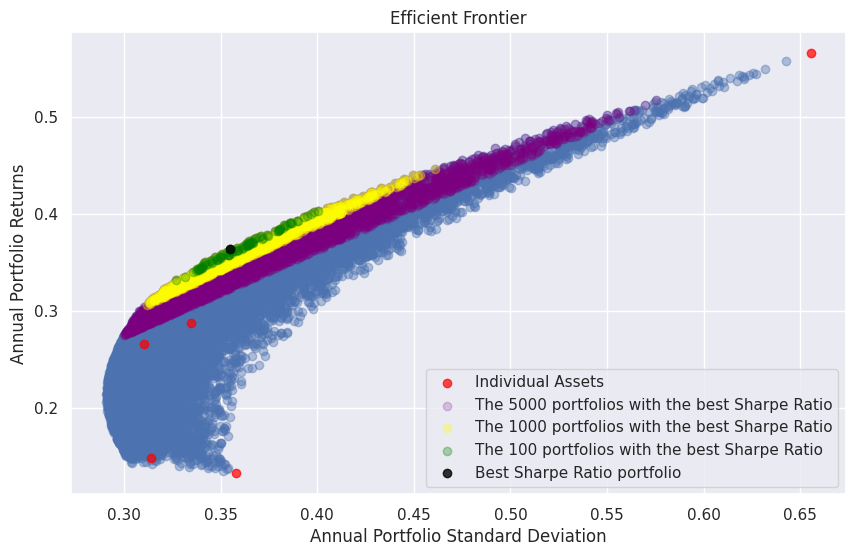
\includegraphics[width=\linewidth,height=0.6\textheight,keepaspectratio]{gfx/m3l2_notes_fig2_efficient_frontier.png}
\par\smallskip{\small \textbf{Hình 2.2:} Đường biên hiệu quả với các danh mục có tỷ số Sharpe cao nhất}
\end{figure}

Về bản chất, những gì ta thấy trong Hình 2.2 chính là đường biên hiệu quả, như đã giải thích trong bài trước, cùng với các danh mục có Tỷ số Sharpe cao nhất được vẽ thêm vào.

Cụ thể hơn, ta minh họa vị trí của 5000, 1000, và 100 danh mục có tỷ số Sharpe cao nhất, và tất nhiên vị trí của danh mục có tỷ số Sharpe tốt nhất. Như dự đoán (?), các danh mục này nằm trên hoặc rất gần đường biên hiệu quả, nhưng bất ngờ là chúng không chiếm toàn bộ đường cong biên hiệu quả.

\textbf{Bài tập 4}

Giải thích vì sao ta kỳ vọng danh mục có tỷ số Sharpe tốt nhất sẽ nằm trên đường biên hiệu quả.

\textbf{Bài tập 5 (để thảo luận)}

Sử dụng dataframe \texttt{highest\_sharpe\_ratio} và in ra 10 danh mục có tỷ số Sharpe cao nhất. Nếu nhìn kỹ vào trọng số, bạn sẽ thấy rằng dù tỷ số Sharpe giữa các danh mục này rất giống nhau, trọng số lại khác nhau nhiều. Ví dụ, trọng số của tài sản thứ nhất trong danh mục thứ 8 là 44.8\%, nhưng trọng số của cùng tài sản đó trong danh mục thứ 7 là 18.7\%. Tuy nhiên, chênh lệch tỷ số Sharpe giữa chúng là rất nhỏ. Hãy suy ngẫm và thảo luận với các bạn học trên diễn đàn về hệ quả của quan sát trên đối với quản lý danh mục đầu tư: rằng nhiều danh mục rất khác nhau lại có tỷ số Sharpe gần như giống hệt nhau.

\section{Danh mục Tiếp tuyến và Đường Tiếp tuyến}

Từ các quan sát trên, giờ ta có thể đưa ra định nghĩa cho danh mục có tỷ số Sharpe tốt nhất: danh mục có tỷ số Sharpe tốt nhất, hay danh mục tiếp tuyến (tangency portfolio), là danh mục tối đa hóa lợi suất trên mỗi đơn vị rủi ro. \textbf{Nó mang lại sự đánh đổi rủi ro-lợi suất tốt nhất trong số tất cả các danh mục} (Elton et al.).

Cuộc thảo luận và minh họa về đường biên hiệu quả của các danh mục cho ta cảm giác rằng đường biên hiệu quả chứa các danh mục tối ưu. Trong mục tiếp theo, ta sẽ thảo luận về đường thị trường vốn (capital market line) để minh họa cách danh mục tiếp tuyến cùng với lãi suất phi rủi ro có thể dùng để tạo ra một chuỗi các danh mục ưu việt hơn đường biên hiệu quả.

Đường tiếp tuyến, hay đường thị trường vốn, là một khái niệm then chốt xuất hiện từ việc kết hợp một tài sản phi rủi ro với danh mục tiếp tuyến. Về mặt toán học, công thức CML là:

$$
r_{\text{CML}} = r_{f} + \frac{r_{T} - r_{f}}{\sigma_{T}} \cdot \sigma_{P}
$$

trong đó
\begin{itemize}
  \item $r_{\text{CML}}$ là lợi suất kỳ vọng của bất kỳ danh mục nào trên CML
  \item $r_{T}$ là lợi suất của danh mục tiếp tuyến (danh mục có tỷ số Sharpe tốt nhất)
  \item $\sigma_{T}$ là độ lệch chuẩn của danh mục tiếp tuyến
  \item $\sigma_{p}$ là độ lệch chuẩn của bất kỳ danh mục nào trên CML
\end{itemize}

Hãy trực quan hóa CML trước khi cung cấp một số trực giác đằng sau việc sử dụng nó:

\begin{lstlisting}[language=Python,escapeinside={(*@}{@*)}]
sigmas = np.linspace(0,0.7, 100)
CML = risk_free_rate + highest_sharpe_ratio['Sharpe Ratio'].iloc[0] * sigmas # (*@Đây@*) (*@là@*) (*@Đường@*) (*@Thị@*) (*@trường@*) (*@Vốn@*)

# (*@Vẽ@*) (*@biểu@*) (*@đồ@*) (*@lợi@*) (*@suất@*) (*@so@*) (*@với@*) (*@phương@*) (*@sai@*) (*@danh@*) (*@mục@*)
plt.figure(figsize = (14,8))
plt.scatter(x = eff_frontier_dataframe['Standard Deviation'], y = eff_frontier_dataframe['Returns'], alpha = 0.4)
plt.scatter(x = r.std() * np.sqrt(252), y = expected_returns, color = 'red', label = "Individual Assets", alpha = 0.7)
plt.scatter(x = highest_sharpe_ratio[:5000]['Standard Deviation'], y = highest_sharpe_ratio[:5000]['Returns'], color = 'purple', alpha = 0.2, label = "The 5000 portfolios with the best Sharpe Ratio" )
plt.scatter(x = highest_sharpe_ratio[:1000]['Standard Deviation'], y = highest_sharpe_ratio[:1000]['Returns'], color = 'yellow', alpha = 0.3, label = "The 1000 portfolios with the best Sharpe Ratio" )
plt.scatter(x = highest_sharpe_ratio[:100]['Standard Deviation'], y = highest_sharpe_ratio[:100]['Returns'], color = 'green', alpha = 0.3, label = "The 100 portfolios with the best Sharpe Ratio" )
plt.scatter(x = highest_sharpe_ratio.iloc[0,:]['Standard Deviation'], y = highest_sharpe_ratio.iloc[0,:]['Returns'], color = 'black', alpha = 0.8, label = "Best Sharpe Ratio portfolio" )
plt.scatter(x = (risk_free / 252).std(), y = risk_free_rate, color = 'black', alpha = 0.8, marker = '*', label = "Risk Free asset", s = 105)
plt.plot(sigmas, CML, color = 'black', label = "Capital Market Line", alpha = 0.7)


plt.title("Efficient Frontier")
plt.xlabel("Annual Portfolio Standard Deviation")
plt.ylabel("Annual Portfolio Returns")
plt.legend()
plt.show()
\end{lstlisting}

\begin{figure}[H]
\centering
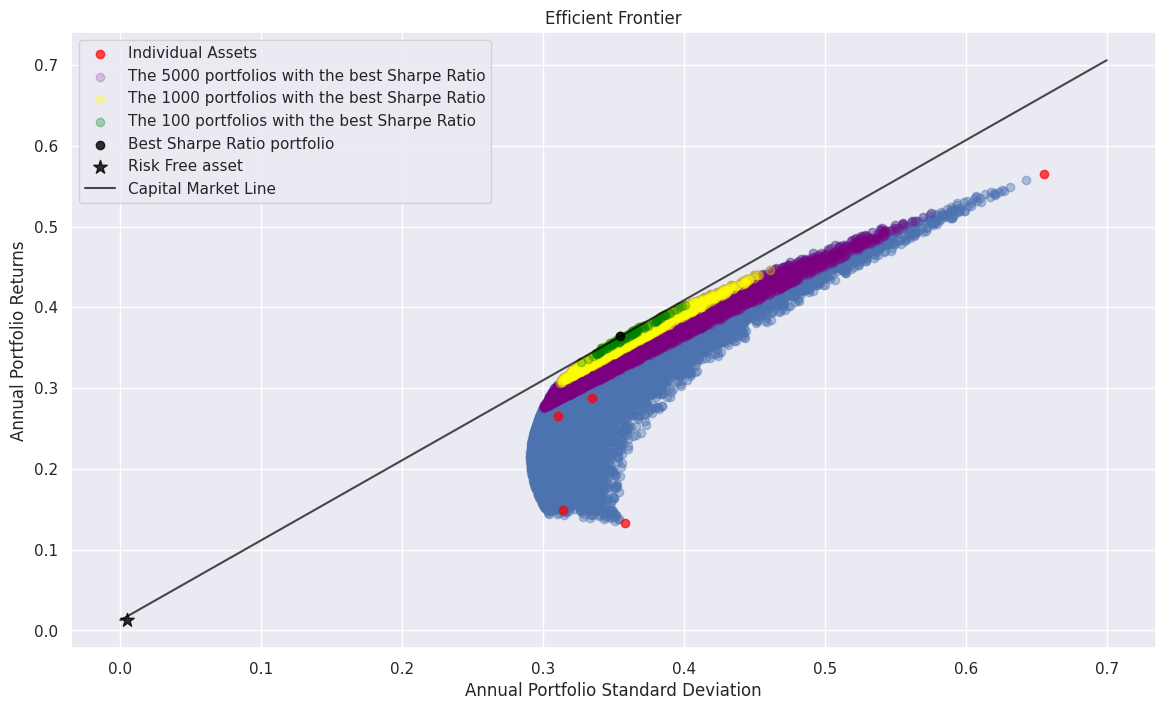
\includegraphics[width=\linewidth,height=0.6\textheight,keepaspectratio]{gfx/m3l2_notes_fig3_efficient_frontier_cml.png}
\par\smallskip{\small \textbf{Hình 2.3:} Đường biên hiệu quả cùng Đường Thị trường Vốn (Capital Market Line) và danh mục tiếp tuyến}
\end{figure}

Trước hết, ta cần quan sát rằng \textbf{độ dốc của đường CML chính là tỷ số Sharpe} của danh mục tiếp tuyến và CML đại diện cho một cải tiến quan trọng so với đường biên hiệu quả. Nhưng các danh mục trên CML được xây dựng thế nào? Hãy sắp xếp lại công thức CML như sau:

$$
r_{\text{CML}} = r_{f} \left ( 1 - \frac{\sigma_{P}}{\sigma_{T}} \right ) + r_{T} \left ( \frac{\sigma_{P}}{\sigma_{T}} \right )
$$

Chỉ đơn giản bằng cách kết hợp tài sản phi rủi ro với danh mục tiếp tuyến và gán các trọng số sau:
\begin{itemize}
  \item Trọng số danh mục tiếp tuyến: $w_{T} = \frac{\sigma_{P}}{\sigma_{T}}$
  \item Trọng số phi rủi ro: $w_{f} = 1 - \frac{\sigma_{P}}{\sigma_{T}}$
\end{itemize}

Sẽ có thêm nội dung về chủ đề này trong môn Quản lý Danh mục Đầu tư.

\section{Value at Risk (VaR)}

Biết phương sai và độ lệch chuẩn là một trợ giúp lớn khi nói đến rủi ro. Điều đó giúp ta tính một trong nhiều cách để đo rủi ro bằng \textbf{Value at Risk}.

Value at Risk là một trong những thước đo rủi ro dễ diễn giải nhất. Cho đến nay, các thước đo ta đã giới thiệu định lượng rủi ro dưới dạng phần trăm, như trường hợp độ lệch chuẩn, hay dưới dạng đơn vị, như tỷ số Sharpe. Value at Risk trả lời câu hỏi cơ bản mà nhiều nhà đầu tư quan tâm: tôi có thể mất bao nhiêu trên một khoản đầu tư trong kịch bản xấu nhất? Trong phạm vi môn học này, giá trị được đo bằng đô la.

Value at Risk đo mức tổn thất tiềm năng về giá trị của một tài sản/danh mục trong một khoảng thời gian xác định. Về cơ bản, bạn luôn cần chỉ rõ khoảng thời gian và khoảng tin cậy đi kèm với một VaR. Ví dụ, nếu VaR của một danh mục là \$1,000,000 trong khoảng thời gian một năm với khoảng tin cậy 99\%, điều đó nghĩa là danh mục chỉ có 1\% khả năng mất hơn \$1,000,000 trong bất kỳ năm nào. VaR đã trở nên phổ biến qua nhiều năm; mọi ngân hàng đầu tư và công ty quản lý rủi ro đều dùng một dạng VaR nào đó để giúp giới hạn mức tổn thất tiềm năng có thể xảy ra. Trọng tâm của VaR chủ yếu là rủi ro sụt giảm (downside risk), khác với thứ như độ lệch chuẩn vốn xem xét cả rủi ro tăng lẫn giảm.

Có ba phương pháp cơ bản để tính VaR, mỗi phương pháp có ưu và nhược điểm riêng. Các phương pháp này dựa trên một số bài học trước đó, như phương sai và hiệp phương sai. Hãy nhớ rằng có vô số biến thể của mỗi phương pháp cơ bản, nhưng chúng ta sẽ chỉ tập trung vào ba phương pháp chính sau:

\begin{itemize}
  \item Phương pháp Lịch sử
  \item Phương pháp Tham số
  \item Mô phỏng Monte Carlo
\end{itemize}

\section{VaR bằng Phương pháp Lịch sử}

Đây có lẽ là phương pháp đơn giản và trực quan nhất để tính Value at Risk. Nói ngắn gọn, lợi suất lịch sử được sắp xếp từ thấp đến cao cho một tài sản hoặc danh mục. Giả sử bạn muốn tính VaR hàng ngày trên một cổ phiếu với khoảng tin cậy 95\%. Giả sử ta có thể xem 1.000 ngày dữ liệu gần nhất cho cổ phiếu này, ta sẽ lấy lợi suất hàng ngày và sắp xếp từ thấp đến cao. Từ đây, ta lấy lợi suất ở phân vị thứ 5 của dữ liệu. Trong trường hợp này, với 1.000 ngày dữ liệu, đó sẽ là lợi suất hàng ngày tệ thứ 50 (0.05*1000) trong số 1.000 ngày này. Giả sử ngày tệ thứ 50 có lợi suất $-4\%$. Từ đó, ta có thể giả định rằng VaR hàng ngày cho cổ phiếu này với khoảng tin cậy 95\% là $-4\%$. Từ đó, nếu ta đầu tư \$1,000 vào cổ phiếu đó, ta sẽ kỳ vọng mức lỗ hàng ngày tệ nhất là:

$$
-0.04 \times 1000 = -\$40 \text{ với khoảng tin cậy 95\%}
$$

Các cân nhắc cho phương pháp này:

\begin{itemize}
  \item Phương pháp này dùng lợi suất lịch sử để đo VaR theo cách thực nghiệm, nghĩa là không có giả định nào về phân phối, trong khi nhiều mô hình khác giả định phân phối chuẩn.
  \item Mỗi ngày trong phương pháp này được cho trọng số bằng nhau, nghĩa là nếu có một xu hướng trong độ biến động, bạn có thể ước tính cao hơn hoặc thấp hơn VaR tùy vào việc xu hướng biến động đang giảm hay tăng. Một cách cải thiện để khắc phục điều này là đặt trọng số lớn hơn cho dữ liệu gần đây hơn.
  \item Dữ liệu quá khứ không nhất thiết cho biết điều gì sẽ xảy ra trong tương lai. Trong khi các phương pháp khác cũng dựa vào dữ liệu lịch sử ở một mức độ nào đó, phương pháp này hoàn toàn suy ra từ lợi suất lịch sử quá khứ. Có nhiều sự kiện không lường trước có thể xảy ra, làm thay đổi quỹ đạo của một cổ phiếu và khiến nó giao dịch khác với trong quá khứ.
\end{itemize}

\subsection{Triển khai Value at Risk (VaR) - Phương pháp Lịch sử}

Tính VaR lịch sử hàng ngày có thể được thực hiện khá đơn giản trong Python. Thứ tự các bước cần thiết như sau:
\begin{enumerate}
  \item Tính tất cả lợi suất hàng ngày.
  \item Sắp xếp các lợi suất này từ nhỏ nhất đến lớn nhất.
  \item Dựa trên một mức tin cậy cho trước, trả về lợi suất ở phân vị tương ứng. Nói cách khác, nếu ta muốn tính VaR hàng ngày ở mức tin cậy 95\% và đang dùng 100 điểm dữ liệu, lợi suất nhỏ thứ 5 của mẫu đó sẽ được coi là VaR 95\% của ta.
\end{enumerate}

Hãy trực quan hóa điều này trước bằng một histogram dùng Bitcoin.

\begin{lstlisting}[language=Python,escapeinside={(*@}{@*)}]
# Figure 1
btcusd = pd.read_csv("btcusd.csv", index_col = "Date", parse_dates = True)
btcusd_returns = btcusd.pct_change().dropna()

plt.hist(x = btcusd_returns, bins=50, log = True, alpha = 0.7)
plt.xlabel('Daily Returns')
plt.ylabel('Frequency')
plt.title('Histogram of BTCUSD Daily Returns')
plt.show()
\end{lstlisting}

\begin{figure}[H]
\centering
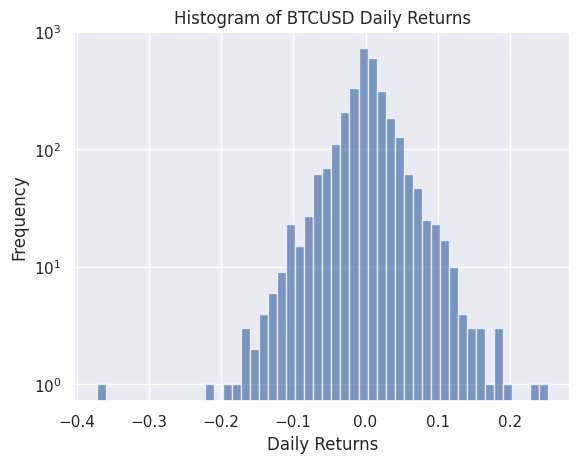
\includegraphics[width=0.75\linewidth]{gfx/m3l2_notes_fig4_btcusd_returns_histogram.png}
\par\smallskip{\small \textbf{Hình 2.4:} Histogram của Lợi suất Hàng ngày BTCUSD}
\end{figure}

Để có hình dung tốt hơn về các sự kiện cực đoan, ta dùng thang logarit cho trục $y$. Hãy tính VaR lịch sử từ dữ liệu này.

Hàm \texttt{getHistoricalVar()} tiếp theo nhận hai đối số:
\begin{enumerate}
  \item một chuỗi lợi suất hàng ngày
  \item một mức tin cậy, ví dụ 95, tương ứng với độ tin cậy 95\%
\end{enumerate}

\begin{lstlisting}[language=Python,escapeinside={(*@}{@*)}]
def getHistoricalVar(returns, confidenceLevel):
    var = np.quantile(returns, 1 - confidenceLevel)
    print(
        f"The Historical VaR with confidence {confidenceLevel} is {round(100 * var, 3)}% \n"
    )

getHistoricalVar(btcusd_returns, 0.90)
getHistoricalVar(btcusd_returns, 0.95)
getHistoricalVar(btcusd_returns, 0.99)
\end{lstlisting}

\begin{lstlisting}[escapeinside={(*@}{@*)}]
The Historical VaR with confidence 0.9 is -3.717%

The Historical VaR with confidence 0.95 is -6.0%

The Historical VaR with confidence 0.99 is -10.57%
\end{lstlisting}

Sau khi chạy hàm này, ta có thể thấy rằng mức tin cậy càng cao, Value at Risk càng thấp. Đây là một công cụ hữu ích khi xác định một tài sản tài chính có thể mất bao nhiêu trong một khoảng thời gian nhất định.

Có lẽ bạn đang tự hỏi, vì ta chỉ dùng mức tin cậy 95\%, điều gì xảy ra vào 5\% số ngày mà mức lỗ vượt quá $-6.02\%$. Ta có thể dùng một thước đo hữu ích khác, Conditional Value at Risk (CVaR), để xử lý các tình huống này.

\subsection{Conditional Value at Risk (CVaR) dùng Dữ liệu Lịch sử}

Conditional Value at Risk (CVaR), còn gọi là Expected Shortfall (ES), là một thước đo rủi ro được sử dụng rộng rãi trong quản lý rủi ro tài chính. Trong khi Value at Risk (VaR) ước lượng mức lỗ trong một khung thời gian cụ thể tại một mức tin cậy cho trước (ví dụ 99\%), CVaR đi xa hơn VaR bằng cách cung cấp mức lỗ kỳ vọng nếu VaR bị vượt qua. Nói cách khác, CVaR tính mức lỗ trung bình ở phần đuôi của phân phối vượt quá ngưỡng VaR.

Về mặt toán học, CVaR ở mức tin cậy $\alpha$ là:

$$
\text{CVaR}_{\alpha} = \mathbb{E}[L|L>\text{VaR}_{\alpha}]
$$

trong đó $L$ đại diện cho mức lỗ.

CVaR lịch sử là một cách tiếp cận phi tham số, nghĩa là nó không dựa vào giả định phân phối cho lợi suất. Thay vào đó, ta có thể tính trực tiếp kỳ vọng của mức lỗ sau khi đã có VaR. Trong thực tế, ta có thể tính trung bình của các lợi suất nằm bên trái VaR.

\begin{lstlisting}[language=Python,escapeinside={(*@}{@*)}]
def getHistoricalCVar(returns, confidenceLevel):
    var = np.quantile(returns, 1 - confidenceLevel)
    cvar = returns[returns <= var].mean()
    print(
        f"With {confidenceLevel} percent confidence VaR, our Expected Shortfall is {round(100 * cvar, 3)} using historical VaR \n"
    )

getHistoricalCVar(btcusd_returns, 0.90)
getHistoricalCVar(btcusd_returns, 0.95)
getHistoricalCVar(btcusd_returns, 0.99)
\end{lstlisting}

% [Ghi chú: notebook gốc chưa chạy cell này nên chưa có output in ra]

\section{VaR bằng Phương pháp Tham số}

VaR tham số là một phương pháp tính Value at Risk giả định rằng lợi suất tuân theo một phân phối xác suất cụ thể. Trong biến thể chuẩn, phân phối chuẩn được giả định, nhưng ta cũng có thể dùng các phân phối khác, như ta sẽ thấy trong ví dụ thứ hai khi giả định phân phối t.

\subsection{VaR Tham số với Phân phối Chuẩn}

Trong trường hợp phân phối chuẩn, việc dùng bảng Z là thiết yếu để tính VaR. Khi thực hiện, ta luôn cần lưu ý rằng rủi ro đề cập đến \textbf{đuôi trái} (left tail).

$$
\text{VaR} = \mu + \sigma Z_{\alpha}
$$

trong đó
\begin{itemize}
  \item $\mu$ là lợi suất trung bình
  \item $\sigma$ là độ lệch chuẩn của lợi suất
  \item $Z_{\alpha}$ là điểm số Z tương ứng với khoảng tin cậy
\end{itemize}

Các cân nhắc cho phương pháp này:

\begin{itemize}
  \item Nếu lợi suất không phân phối chuẩn, khả năng cao bạn sẽ ước tính thấp Value at Risk thực. Ví dụ, nhiều cổ phiếu có nhiều giá trị ngoại lai hơn so với giả định của phân phối chuẩn; điều này nghĩa là Value at Risk tính được sẽ thấp hơn thực tế.
  \item Phương sai và hiệp phương sai giữa các chuỗi lợi suất phải được tính đến khi tính VaR cho một danh mục. Ngay cả khi lợi suất phân phối chuẩn, phép tính VaR vẫn có thể sai lệch nếu phương sai và hiệp phương sai ước lượng không chính xác. Điều này có thể bị khuếch đại hơn nếu phương sai và hiệp phương sai thay đổi theo thời gian.
  \item Các mô hình cho phép phương sai thay đổi theo thời gian (phương sai không đồng nhất, heteroskedasticity) thể hiện độ chính xác cao hơn. Engle đã lập luận rằng các mô hình tự hồi quy phương sai có điều kiện (ARCH) và tổng quát hóa (GARCH) cho dự báo phương sai tốt hơn, và do đó, thước đo Value at Risk tốt hơn.
  \item Phương pháp này bị phá vỡ bất cứ khi nào danh mục có tài sản với cấu trúc lợi nhuận phi tuyến tính, ví dụ quyền chọn.
\end{itemize}

\subsection{Triển khai VaR Tham số với Phân phối Chuẩn}

Mặc dù đã được biết rõ rằng lợi suất tài chính, đặc biệt với cổ phiếu, thường thể hiện các đặc điểm phi chuẩn, như độ lệch (skewness) và đuôi béo (fat tails), phương pháp tham số này vẫn có giá trị đáng kể trong quản lý rủi ro tài chính. Giả định phân phối chuẩn cung cấp một cách hiệu quả để ước lượng rủi ro, khiến nó rất hữu ích trong các tình huống cần xấp xỉ nhanh hoặc có thể dùng kết hợp với các mô hình khác.

Để tính Value at Risk (VaR) bằng phương pháp tham số, ta sẽ dùng hàm \texttt{norm.ppf()} từ mô-đun \texttt{scipy.stats} của Python. Hàm điểm phần trăm (percent point function, ppf) thực chất là hàm phân phối tích lũy nghịch đảo (inverse CDF), cho phép ta tính phân vị tương ứng với một mức tin cậy cho trước.

\begin{lstlisting}[language=Python,escapeinside={(*@}{@*)}]
mean = btcusd_returns.mean()
std = btcusd_returns.std()

var_90 = stats.norm.ppf(0.1, mean, std)[0]
var_95 = stats.norm.ppf(0.05, mean, std)[0]
var_99 = stats.norm.ppf(0.01, mean, std)[0]

print(f"The parametric VaR assuming a normal distribution with a 90% confidence interval, is {round(100 * var_90, 3)} \n")
print(f"The parametric VaR assuming a normal distribution with a 95% confidence interval, is {round(100 * var_95, 3)} \n")
print(f"The parametric VaR assuming a normal distribution with a 99% confidence interval, is {round(100 * var_99, 3)} \n")
\end{lstlisting}

% [Ghi chú: notebook gốc chưa chạy cell này nên chưa có output in ra]

Độ nhọn dư (excess kurtosis) quan sát được trong phân phối lợi suất tài sản cho thấy phân phối chuẩn không phải lựa chọn tốt nhất để đại diện cho lợi suất, đặc biệt ở phần đuôi. Bản chất đuôi béo của chúng cho thấy xác suất cao hơn của các kết quả cực đoan, trong nhiều trường hợp cao hơn nhiều so với những gì phân phối chuẩn dự đoán. Điều này buộc ta phải dùng một phân phối đuôi nặng như phân phối t Student.

\textbf{Bài tập 6}

Tính Độ nhọn (Kurtosis) của lợi suất BTCUSD và đảm bảo bạn hiểu ảnh hưởng của độ nhọn cao lên phần đuôi. Sau đó lập luận về lý do phân phối chuẩn có vẻ ước tính thấp VaR so với phương pháp lịch sử.

\textbf{Bài tập 7 (thảo luận)}

Xem histogram BTCUSD trình bày ở Hình 2.4. Đảm bảo bạn cũng in ra 10 lợi suất đầu tiên sau khi sắp xếp chúng với \texttt{ascending = True}. Trình bày chi tiết về các khoảng trống giữa các lợi suất (như các điểm dữ liệu) ở đuôi trái: mẫu của chúng ta có đại diện đầy đủ cho đuôi trái hay không?

Trong mục tiếp theo, ta sẽ đi sâu vào cách phân phối t Student có thể được sử dụng trong tính toán Value at Risk (VaR), mang lại một đánh giá rủi ro chính xác hơn cho các tài sản thể hiện đuôi béo.

\subsection{Triển khai VaR Tham số với phân phối $t$}

Phân phối t Student thường được dùng như một lựa chọn thay thế cho phân phối chuẩn khi mô hình hóa dữ liệu có đuôi béo. Tham số bậc tự do (degrees of freedom) kiểm soát độ "nặng" của đuôi. Khi bậc tự do tăng, phân phối t tiệm cận phân phối chuẩn. Với bậc tự do (dof) nhỏ hơn, đuôi trở nên nặng hơn, cho thấy xác suất cao hơn của các giá trị cực đoan.

\begin{lstlisting}[language=Python,escapeinside={(*@}{@*)}]
# (*@Bậc@*) (*@tự@*) (*@do@*)

def getTVar(returns, dof, confidenceLevel):
    mean = returns.mean()
    std = returns.std()
    var = np.sqrt((dof - 2) / dof) * stats.t.ppf(1 - confidenceLevel, dof) * std + mean
    return (100 * var).round(3)

print(f"The parametric VaR using t-distribution with a confidence interval 0.9, is {getTVar(btcusd_returns, 5, 0.9)}% \n")
print(f"The parametric VaR using t-distribution with a confidence interval 0.95, is {getTVar(btcusd_returns, 5, 0.95)}% \n")
print(f"The parametric VaR using t-distribution with a confidence interval 0.99, is {getTVar(btcusd_returns, 5, 0.99)}% \n")
\end{lstlisting}

% [Ghi chú: notebook gốc chưa chạy cell này nên chưa có output in ra]

\section{VaR bằng Mô phỏng Monte Carlo}

Trong các mục trước, ta đã thảo luận cách sử dụng dữ liệu lịch sử trên các chuỗi tài chính để tính Value at Risk. Nhưng nếu ta có dữ liệu không đầy đủ hoặc không đủ để làm điều đó thì sao? Trong trường hợp này, ta có thể giả thuyết một phân phối tạo ra dữ liệu và chạy mô phỏng dùng các giả định phân phối đó. Phương pháp này được gọi là \emph{Monte Carlo VaR}.

Monte Carlo VaR bao gồm một chuỗi mô phỏng, trong đó mỗi chuỗi lợi suất được biểu diễn dưới dạng một biến ngẫu nhiên. Biến này có thể được lấy từ bất kỳ phân phối xác suất nào, điều này rất tốt vì có nghĩa là nó không nhất thiết giả định phân phối chuẩn. Có rất nhiều linh hoạt trong việc chọn loại phân phối để dùng. Tất cả các biến sau đó được gán trọng số theo đô la và mô phỏng để xem tổng giá trị danh mục là bao nhiêu vào cuối mỗi lần chạy. Các lợi suất mô phỏng này sau đó được sắp xếp từ thấp đến cao, và ta có thể dễ dàng xem Value at Risk là bao nhiêu bằng các phép tính tương tự phương pháp lịch sử, ngoại trừ lần này ta dùng lợi suất mô phỏng thay vì lợi suất lịch sử. Ví dụ, nếu bạn chạy một chuỗi 1.000 mô phỏng, bạn sẽ xem giá trị thấp thứ 50 để xác định VaR cho khoảng tin cậy 95\%.

Các cân nhắc cho phương pháp này:
\begin{itemize}
  \item Các ước lượng sẽ không hiệu quả nếu phân phối xác suất dùng để xác định các biến ngẫu nhiên không chính xác. Nhiều người dùng dữ liệu quá khứ để có ý tưởng về phân phối xác suất nên dùng; phương pháp này cho phép một mức độ chủ quan nhất định.
  \item Bạn có thể ước lượng VaR hiệu quả hơn cho các danh mục chứa quyền chọn bằng phương pháp này so với phương pháp tham số, vì Monte Carlo không giả định lợi suất phân phối chuẩn.
\end{itemize}

\section{Kết luận}

Trong bài học này, chúng ta đã giới thiệu một loạt các khái niệm quan trọng trong phân tích rủi ro tài chính. Chúng ta bắt đầu bằng việc xem xét các loại lợi suất khác nhau, bao gồm tổng lợi suất, lợi suất điều chỉnh cổ tức, và lợi suất vượt trội, tạo nền tảng cho các thước đo rủi ro nâng cao hơn. Sau đó ta khám phá Tỷ số Sharpe và minh họa tầm quan trọng của tỷ số này trong bối cảnh quản lý danh mục đầu tư.

Phần sau của bài học tập trung vào các thước đo rủi ro sụt giảm (downside risk), đặc biệt là Value at Risk (VaR). Chúng ta đã đề cập nhiều phương pháp tính VaR, bao gồm lịch sử, tham số (với cả phân phối chuẩn và phân phối t), và phương pháp mô phỏng Monte Carlo. Chúng ta cũng đã giới thiệu khái niệm Conditional Value at Risk (CVaR) như một mở rộng của VaR.

\textbf{Tài liệu tham khảo}

\begin{itemize}
  \item Elton, Edwin J., et al. \emph{Modern Portfolio Theory and Investment Analysis}. John Wiley \& Sons, 2009.
  \item Engle, Robert. "GARCH 101: The Use of ARCH/GARCH Models in Applied Econometrics." \emph{The Journal of Economic Perspectives}, vol. 15, no. 4, 2001, pp. 157--168.
\end{itemize}

\chapter{Đọc thêm: Mô hình CAPM và Đo lường Hiệu suất (Dahlquist \& Knight)}
\label{ch:M3L2-reading1}

% Nguồn: Dahlquist, Julie, and Rainford Knight. "Principles of Finance." OpenStax, 2022.
% Phần cần đọc: Section 15.3 (The Capital Asset Pricing Model) & 15.4 (Applications in Performance Measurement)
% Nội dung bắt buộc đọc: được kiểm tra trong mọi bài đánh giá (kể cả Quiz).

\section{Thông tin nguồn}

\begin{itemize}
  \item \textbf{Nguồn:} Dahlquist, Julie, and Rainford Knight. \emph{Principles of Finance}. OpenStax Press, 2022. (truy cập mở tại \url{https://openstax.org/details/books/principles-finance})
  \item \textbf{Phần cần đọc:} Section 15.3: The Capital Asset Pricing Model (CAPM); Section 15.4: Applications in Performance Measurement
\end{itemize}

\section{15.3 Mô hình Định giá Tài sản Vốn (CAPM)}

\subsection*{Mục tiêu học tập}
Sau khi hoàn thành mục này, bạn sẽ có thể:
\begin{itemize}
  \item Định nghĩa phần bù rủi ro (risk premium).
  \item Giải thích khái niệm beta.
  \item Tính lợi suất yêu cầu của một chứng khoán bằng CAPM.
\end{itemize}

\subsection*{Lãi suất Phi rủi ro}

Mô hình định giá tài sản vốn (capital asset pricing model, CAPM) là một lý thuyết tài chính dựa trên ý tưởng rằng nhà đầu tư sẵn sàng nắm giữ cổ phiếu có rủi ro hệ thống cao hơn nên được thưởng nhiều hơn khi chấp nhận rủi ro thị trường này. CAPM tập trung vào rủi ro hệ thống, thay vì rủi ro riêng của từng cổ phiếu, vì rủi ro đặc thù doanh nghiệp có thể loại bỏ thông qua đa dạng hóa.

Giả sử ông bà bạn tặng bạn \$20,000. Sau khi tốt nghiệp đại học, bạn dự định đi làm vài năm rồi nộp đơn vào trường luật. Bạn muốn dùng \$20,000 ông bà cho để trả một phần học phí trường luật. Sẽ mất vài năm trước khi bạn sẵn sàng tiêu số tiền đó, và bạn muốn giữ nó an toàn. Đồng thời, bạn muốn đầu tư số tiền và để nó tăng trưởng cho đến khi bạn sẵn sàng vào trường luật.

Mặc dù bạn muốn kiếm lợi suất trên số tiền để có nhiều hơn \$20,000 vào lúc bắt đầu trường luật, mục tiêu chính của bạn là giữ tiền an toàn. Bạn đang tìm một khoản đầu tư phi rủi ro. Cho chính phủ Mỹ vay tiền được coi là khoản đầu tư rủi ro thấp nhất bạn có thể thực hiện. Bạn có thể mua một chứng khoán Kho bạc Mỹ. Khả năng chính phủ Mỹ không trả được nợ gần như bằng 0. Mặc dù về lý thuyết, không khoản đầu tư nào an toàn 100\%, đầu tư vào chứng khoán chính phủ Mỹ nhìn chung được coi là một khoản đầu tư phi rủi ro vì rủi ro cực kỳ nhỏ.

Lãi suất bạn có thể kiếm được bằng cách mua chứng khoán Kho bạc Mỹ là một đại diện cho lãi suất phi rủi ro. Nó được dùng làm chuẩn đầu tư. Lãi suất trung bình cho tín phiếu Kho bạc Mỹ 3 tháng từ 1928 đến 2020 là 3.36\%. Bạn có thể thấy rằng bạn sẽ không trở nên giàu có nhờ đầu tư vào tín phiếu Kho bạc Mỹ. Tuy nhiên, một đặc điểm khác của chứng khoán Kho bạc Mỹ là độ biến động của chúng có xu hướng thấp hơn nhiều so với cổ phiếu. Thực tế, độ lệch chuẩn của lợi suất tín phiếu Kho bạc Mỹ là 3.0\%. Khác với lợi suất cổ phiếu, lợi suất tín phiếu Kho bạc Mỹ chưa bao giờ âm. Lợi suất hàng năm thấp nhất là 0.03\%, xảy ra vào năm 2014.

\subsection*{Phần bù Rủi ro}

Bạn biết rằng nếu dùng \$20,000 để đầu tư vào cổ phiếu thay vì tín phiếu Kho bạc Mỹ, kết quả đầu tư sẽ không chắc chắn. Khoản đầu tư của bạn có thể sinh lời tốt, nhưng cũng có rủi ro mất tiền. Bạn sẽ chỉ sẵn sàng chấp nhận rủi ro này nếu được đền bù xứng đáng. Nói cách khác, bạn sẽ chỉ sẵn sàng chấp nhận rủi ro đầu tư vào cổ phiếu nếu bạn nghĩ rằng làm vậy sẽ mang lại nhiều tiền hơn so với đầu tư vào chứng khoán Kho bạc Mỹ.

Từ 1928 đến 2020, lợi suất trung bình của chỉ số cổ phiếu S\&P 500 là 11.64\%, cao hơn nhiều so với lợi suất trung bình 3.36\% của tín phiếu Kho bạc Mỹ. Tuy nhiên, lợi suất cổ phiếu, với độ lệch chuẩn 19.49\%, cũng biến động nhiều hơn nhiều. Thực tế, có 25 năm mà lợi suất của chỉ số S\&P 500 âm.

Bạn có thể không muốn chấp nhận rủi ro mất một phần số tiền ông bà đã cho vì bạn đang để dành nó cho trường luật. Nếu vậy, bạn sẽ muốn đầu tư vào chứng khoán Kho bạc Mỹ. Bạn có thể có tiền để dành cho các mục tiêu dài hạn khác, như nghỉ hưu, mà bạn sẵn sàng chấp nhận một số rủi ro. Lợi suất thêm mà bạn kiếm được khi chấp nhận rủi ro được gọi là phần bù rủi ro (risk premium). Phần bù rủi ro có thể được hiểu là phần thưởng cho việc bạn sẵn sàng gánh chịu rủi ro.

Phần bù rủi ro được tính bằng chênh lệch giữa lợi suất bạn nhận được khi chấp nhận rủi ro và lợi suất bạn sẽ nhận được nếu không chấp nhận rủi ro. Dùng lợi suất trung bình của S\&P 500 (để đo những gì nhà đầu tư chấp nhận rủi ro kiếm được) và lãi suất tín phiếu Kho bạc Mỹ (để đo những gì nhà đầu tư không chấp nhận rủi ro kiếm được), phần bù rủi ro được tính là:

$$
\text{Phần bù rủi ro} = 11.64\% - 3.36\% = 8.28\%
$$

\subsection*{Beta}

Phần bù rủi ro đại diện cho mức một nhà đầu tư nắm giữ danh mục thị trường được thưởng cho rủi ro. Nhà đầu tư mua một cổ phiếu, ví dụ DAL, trải nghiệm độ biến động, được đo bằng độ lệch chuẩn của lợi suất cổ phiếu đó. Hãy nhớ rằng một phần độ biến động đó, độ biến động gây ra bởi rủi ro đặc thù doanh nghiệp, có thể được loại bỏ thông qua đa dạng hóa. Vì nhà đầu tư có thể loại bỏ rủi ro đặc thù doanh nghiệp thông qua đa dạng hóa, họ sẽ không được thưởng cho rủi ro đó. Nhà đầu tư được thưởng cho lượng rủi ro hệ thống họ gánh chịu.

\subsection*{Diễn giải Beta}

Rủi ro liên quan đối với nhà đầu tư là rủi ro hệ thống họ gánh chịu. Rủi ro hệ thống của một cổ phiếu cụ thể được đo bằng mức độ cổ phiếu đó di chuyển cùng thị trường. Thước đo mức độ một cổ phiếu di chuyển cùng thị trường được gọi là beta của nó. Một cổ phiếu có xu hướng di chuyển đồng bộ với thị trường sẽ có beta bằng 1. Với các cổ phiếu này, nếu thị trường tăng 10\%, cổ phiếu nhìn chung cũng tăng 10\%; nếu thị trường giảm 5\%, cổ phiếu có beta bằng 1 cũng có xu hướng giảm 5\%.

Nếu một công ty có beta lớn hơn 1, cổ phiếu có xu hướng di chuyển mạnh hơn theo cùng hướng với thị trường. Ví dụ, nếu một cổ phiếu có beta bằng 2, cổ phiếu sẽ có xu hướng tăng 20\% khi thị trường tăng 10\%. Nếu thị trường giảm 5\%, cùng cổ phiếu đó sẽ có xu hướng giảm gấp đôi, tức 10\%. Do đó, cổ phiếu có beta lớn hơn 1 trải qua biến động lớn hơn thị trường chung và được coi là rủi ro hơn cổ phiếu trung bình.

Mặt khác, cổ phiếu có beta nhỏ hơn 1 trải qua biến động nhỏ hơn thị trường chung. Ví dụ, beta bằng 0.5 nghĩa là cổ phiếu có xu hướng biến động chỉ bằng 50\% biến động thị trường chung. Vậy, nếu thị trường tăng 10\%, cổ phiếu có beta 0.5 sẽ có xu hướng tăng chỉ 5\%. Thị trường giảm 5\% sẽ có xu hướng gắn với mức giảm 2.5\% của cổ phiếu.

\subsection*{Tính Beta}

Phép tính beta cho DAL được minh họa trong Hình 15.3. Lợi suất hàng tháng của DAL và S\&P 500 được vẽ trên biểu đồ. Mỗi điểm trong biểu đồ phân tán tương ứng với một tháng từ 2018 đến 2020; ví dụ, điểm nằm xa nhất ở góc trên bên phải đại diện cho tháng 11/2020. Lợi suất của S\&P 500 tháng đó là 10.88\%; lợi suất này được vẽ trên trục ngang. Lợi suất của DAL trong tháng 11/2020 là 31.36\%; lợi suất này được vẽ trên trục dọc.

Bạn có thể thấy rằng nhìn chung, khi toàn bộ thị trường chứng khoán đo bằng S\&P 500 dương, lợi suất của DAL cũng dương. Tương tự, trong các tháng mà lợi suất S\&P 500 âm, lợi suất của DAL cũng thường âm. Vẽ một đường khớp nhất với dữ liệu, còn gọi là đường hồi quy, tóm tắt mối quan hệ giữa lợi suất của DAL và S\&P 500. Độ dốc của đường này, 1.39, chính là beta của DAL. Beta đo lượng rủi ro hệ thống mà DAL có.

\begin{figure}[H]
\centering
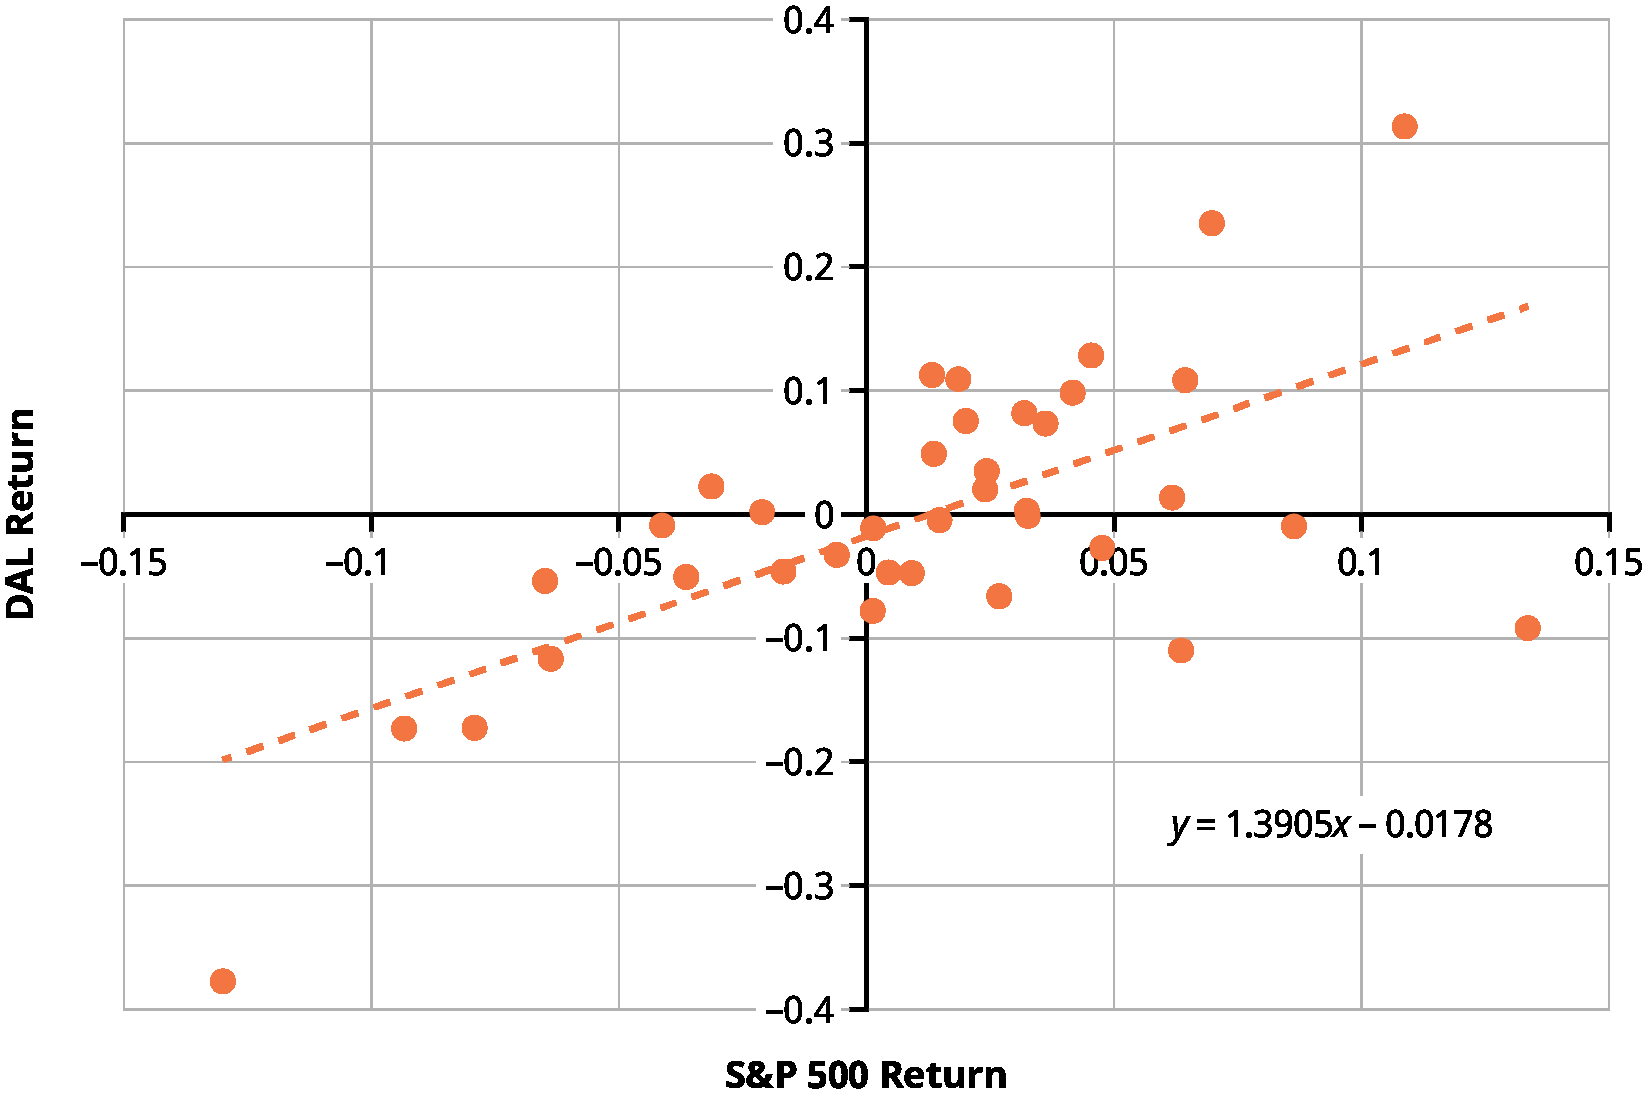
\includegraphics[width=0.7\linewidth]{gfx/m3l2_dahlquist_fig15-3_beta_calc.png}
\par\smallskip{\small \textbf{Hình 15.3:} Tính Beta cho DAL (nguồn dữ liệu: Yahoo! Finance)}
\end{figure}

\subsection*{Công thức CAPM}

Vì beta 1.39 của DAL lớn hơn 1, DAL rủi ro hơn cổ phiếu trung bình trên thị trường. Lý thuyết tài chính cho thấy nhà đầu tư mua DAL sẽ kỳ vọng một tỷ lệ lợi suất cao hơn để đền bù cho rủi ro này. DAL có 139\% rủi ro hệ thống của cổ phiếu trung bình; do đó, nhà đầu tư vào cổ phiếu này nên nhận 139\% phần bù rủi ro thị trường.

Công thức mô hình định giá tài sản vốn (CAPM) là

$$
R_e = R_f + \beta (R_m - R_f)
$$

trong đó $R_e$ là lợi suất kỳ vọng của tài sản, $R_f$ là lãi suất phi rủi ro, và $R_m$ là lợi suất kỳ vọng của thị trường. Với lợi suất trung bình S\&P 500 là 11.64\% và lợi suất trung bình tín phiếu Kho bạc Mỹ là 3.36\%, lợi suất kỳ vọng của DAL sẽ được tính là:

$$
R_e = 3.36\% + 1.39 \times (11.64\% - 3.36\%) = 14.87\%
$$

\begin{framed}
\textbf{LIÊN KẾT ĐẾN VIỆC HỌC: Tính Beta}

Nhiều nhà cung cấp dữ liệu cổ phiếu và thông tin đầu tư sẽ liệt kê beta của một công ty. Các nguồn khác nhau có thể không đưa ra cùng một giá trị beta cho một công ty. Ví dụ, vào đầu tháng 2/2021, Yahoo! Finance báo cáo beta của DAL là 1.46, trong khi MarketWatch báo cáo là 1.29. Cả hai con số này đều hơi khác so với 1.39 tính được trong biểu đồ ở trên.

Có một số lý do khiến beta có thể hơi khác nhau giữa các nguồn. Một là khung thời gian dùng trong phép tính beta. Dữ liệu ba năm được dùng để tính beta trong Hình 15.3. Khung thời gian từ ba đến năm năm thường được dùng khi tính beta. Một lý do khác khiến các nguồn khác nhau có thể báo cáo beta khác nhau là tần suất thu thập dữ liệu. Lợi suất hàng tháng được dùng trong Hình 15.3; một số nhà phân tích sẽ dùng dữ liệu hàng tuần. Cuối cùng, S\&P 500 được dùng để đo lợi suất thị trường trong Hình 15.3; S\&P 500 là một trong những thước đo phổ biến nhất về lợi suất thị trường chung, nhưng vẫn có các lựa chọn thay thế được một số nhà phân tích sử dụng.
\end{framed}

\section{15.4 Ứng dụng trong Đo lường Hiệu suất}

\subsection*{Mục tiêu học tập}
Sau khi hoàn thành mục này, bạn sẽ có thể:
\begin{itemize}
  \item Diễn giải tỷ số Sharpe.
  \item Diễn giải phép đo Treynor.
  \item Diễn giải alpha Jensen.
\end{itemize}

\subsection*{Tỷ số Sharpe}

Nhà đầu tư muốn một thước đo về mức độ giỏi của một nhà quản lý tiền chuyên nghiệp trước khi giao phó số tiền khó nhọc kiếm được của mình cho người đó đầu tư. Giả sử bạn thấy một quảng cáo trong đó McKinley Investment Management tuyên bố rằng danh mục của khách hàng họ có lợi suất trung bình 20\% mỗi năm. Bạn biết rằng lợi suất trung bình hàng năm này vô nghĩa nếu không biết thêm về mức độ rủi ro của chiến lược công ty. Trong mục này, ta xem xét một số cách đánh giá mức độ rủi ro của một chiến lược đầu tư.

Một thước đo cơ bản về hiệu suất đầu tư có điều chỉnh rủi ro là tỷ số Sharpe. Tỷ số Sharpe được tính bằng phần bù rủi ro của danh mục chia cho độ lệch chuẩn của lợi suất danh mục, dùng công thức:

$$
\text{Sharpe Ratio} = \frac{R_P - R_f}{\sigma_P}
$$

Phần bù rủi ro của danh mục là lợi suất danh mục $R_P$ trừ lợi suất phi rủi ro $R_f$; đây là phần thưởng cơ bản cho việc gánh chịu rủi ro. Nếu lợi suất phi rủi ro là 3\%, khách hàng của McKinley Investment Management kiếm được 20\% trên danh mục của họ có lợi suất vượt trội 17\%.

Độ lệch chuẩn của lợi suất danh mục, $\sigma_P$, là một thước đo rủi ro. Mặc dù bạn thấy khách hàng của McKinley kiếm được lợi suất trung bình khá tốt là 20\%, bạn nhận ra lợi suất rất biến động. Trong một số năm, khách hàng kiếm được nhiều hơn 20\%, và trong các năm khác, lợi suất thấp hơn nhiều, thậm chí âm. Độ biến động đó dẫn đến độ lệch chuẩn của lợi suất là 26\%. Tỷ số Sharpe sẽ là $17\%/26\% = 0.65$.

Như vậy, tỷ số Sharpe có thể được hiểu là tỷ số phần thưởng trên rủi ro. Độ lệch chuẩn ở mẫu số có thể được hiểu là đơn vị rủi ro mà nhà đầu tư gánh chịu. Tử số là phần thưởng nhà đầu tư nhận được khi chấp nhận rủi ro đó.

\begin{framed}
\textbf{LIÊN KẾT ĐẾN VIỆC HỌC: Tỷ số Sharpe}

Tỷ số Sharpe được phát triển bởi người đạt giải Nobel William F. Sharpe. Bạn có thể truy cập trang web của Sharpe tại Đại học Stanford để tìm các video trong đó ông thảo luận về các chủ đề tài chính và liên kết đến nghiên cứu của ông cũng như lời khuyên của ông về cách đầu tư.
\end{framed}

\subsection*{Phép đo Hiệu suất Treynor}

Một thước đo tỷ số phần thưởng trên rủi ro khác về hiệu suất đầu tư là tỷ số Treynor. Tỷ số Treynor được tính là:

$$
\text{Treynor Ratio} = \frac{R_P - R_f}{\beta_P}
$$

Cũng như tỷ số Sharpe, tử số của tỷ số Treynor là phần bù rủi ro của danh mục; điểm khác biệt là tỷ số Treynor tập trung vào rủi ro hệ thống, dùng beta của danh mục ở mẫu số, trong khi tỷ số Sharpe tập trung vào tổng rủi ro, dùng độ lệch chuẩn của lợi suất danh mục ở mẫu số.

Nếu McKinley Investment Management có một danh mục với lợi suất 20\% trong năm năm qua, với beta 1.2 và lãi suất phi rủi ro 3\%, tỷ số Treynor sẽ là:

$$
\text{Treynor Ratio} = \frac{20\% - 3\%}{1.2} = 14.17\%
$$

Cả tỷ số Sharpe và Treynor đều là thước đo tương đối về hiệu suất đầu tư, nghĩa là không có một con số tuyệt đối cho biết hiệu suất đầu tư là tốt hay xấu. Hiệu suất của một nhà quản lý đầu tư phải được xem xét trong tương quan với các nhà quản lý khác hoặc với một chỉ số chuẩn tham chiếu.

\subsection*{Alpha Jensen}

Alpha Jensen là một thước đo phổ biến khác về hiệu suất đầu tư. Nó được tính bằng lợi suất danh mục thô trừ đi lợi suất danh mục kỳ vọng dự đoán bởi CAPM:

$$
\alpha = R_P - \left[ R_f + \beta_P (R_m - R_f) \right]
$$

Giả sử lợi suất thị trường trung bình là 12\%. Alpha Jensen sẽ là bao nhiêu cho danh mục của McKinley Investment Management với lợi suất trung bình 20\% và beta 1.2?

$$
\alpha = 20\% - \left[ 3\% + 1.2 \times (12\% - 3\%) \right] = 20\% - 13.8\% = 6.2\%
$$

Khác với tỷ số Sharpe và Treynor, vốn có ý nghĩa theo nghĩa tương đối, alpha Jensen có ý nghĩa theo nghĩa tuyệt đối. Alpha bằng 0.062 cho thấy danh mục McKinley Investment Management mang lại lợi suất cao hơn 6.2\% so với kỳ vọng dựa trên mức độ rủi ro của danh mục. Alpha dương cho thấy danh mục có lợi suất bất thường (abnormal return). Nếu alpha Jensen bằng 0, lợi suất danh mục đúng bằng những gì được kỳ vọng dựa trên mức độ rủi ro của danh mục đo bằng beta.

\begin{framed}
\textbf{THỰC HÀNH: So sánh Lợi suất và Rủi ro của các Danh mục}

Bạn đang phỏng vấn hai nhà quản lý đầu tư. Ông Wong cho thấy lợi suất trung bình trên danh mục của ông trong 10 năm qua là 14\%, với độ lệch chuẩn 8\% và beta 1.2. Bà Petrov cho thấy lợi suất trung bình trên danh mục của bà trong 10 năm qua là 16\%, với độ lệch chuẩn 10\% và beta 1.6. Bạn biết rằng trong 10 năm qua, lãi suất chứng khoán Kho bạc Mỹ trung bình là 2\% và lợi suất S\&P 500 trung bình là 11\%. Bạn nghĩ nhà quản lý danh mục nào đã làm tốt hơn?

\textbf{Lời giải:}

Tỷ số Sharpe cho danh mục của ông Wong là $(14\%-2\%)/8\% = 1.5$, và tỷ số Treynor là $(14\%-2\%)/1.2 = 10\%$. Tỷ số Sharpe cho danh mục của bà Petrov là $(16\%-2\%)/10\% = 1.4$, và tỷ số Treynor là $(16\%-2\%)/1.6 = 8.75\%$.

Alpha Jensen cho danh mục của ông Wong là $14\% - [2\% + 1.2\times(11\%-2\%)] = 1.2\%$.

Alpha Jensen cho danh mục của bà Petrov là $16\% - [2\% + 1.6\times(11\%-2\%)] = -0.4\%$.

Cả ba thước đo hiệu suất danh mục đều cho thấy danh mục của ông Wong hoạt động tốt hơn danh mục của bà Petrov. Mặc dù bà Petrov có lợi suất trung bình lớn hơn, danh mục bà quản lý lại rủi ro hơn. Danh mục của bà Petrov biến động hơn danh mục của ông Wong, dẫn đến độ lệch chuẩn cao hơn. Danh mục của bà Petrov có beta cao hơn, nghĩa là nó có lượng rủi ro hệ thống cao hơn. CAPM cho thấy một danh mục với beta 1.6 nên có lợi suất kỳ vọng 16.4\%. Vì danh mục của bà Petrov có lợi suất trung bình thấp hơn mức đó, nhà đầu tư vào danh mục của bà Petrov không được đền bù cho rủi ro họ đã chấp nhận nhiều như kỳ vọng.
\end{framed}

\chapter{Đọc thêm: Các Thước đo Rủi ro dựa trên Phân vị (Dowd \& Blake)}
\label{ch:M3L2-reading2}

% Nguồn: Dowd, Kevin, and David Blake. "After VaR: The Theory, Estimation, and Insurance Applications of Quantile-Based Risk Measures." Journal of Risk and Insurance, vol. 73, no. 2, 2006, pp. 193-229.
% Phần cần đọc: Sections 2.1-2.4 (Quantile-Based Measures of Risk) & 3.1-3.3 (Estimation Methods)
% Nội dung bắt buộc đọc: được kiểm tra trong mọi bài đánh giá (kể cả Quiz).

\section{Thông tin nguồn}

\begin{itemize}
  \item \textbf{Nguồn:} Dowd, Kevin, and David Blake. "After VaR: The Theory, Estimation, and Insurance Applications of Quantile-Based Risk Measures." \emph{Journal of Risk and Insurance}, vol. 73, no. 2, 2006, pp. 193--229. \url{https://dhenriet.perso.centrale-med.fr/var2.pdf}
  \item \textbf{Phần cần đọc:} Sections 2.1--2.4 và 3.1--3.3
\end{itemize}

\section{Các Thước đo Rủi ro dựa trên Phân vị (Quantile-Based Measures of Risk)}

\subsection{Value at Risk}

Về mặt thực tiễn, ta có thể truy nguồn gốc của VaR về cuối thập niên 1970 và 1980, khi một số định chế tài chính lớn bắt đầu xây dựng các mô hình dự báo rủi ro nội bộ để đo lường và tổng hợp rủi ro trên toàn định chế.\footnote{Gốc rễ của thước đo này còn xa hơn nữa. Có thể lập luận rằng VaR đã hàm chứa trong thước đo dự trữ ban đầu xuất hiện trong bài toán xác suất phá sản cổ điển mà các nhà tính toán bảo hiểm (actuary) đã quen thuộc từ đầu thế kỷ 20. VaR cũng có thể được quy về Baumol (1963), người đề xuất một thước đo rủi ro bằng $\mu - k\sigma$. Tuy nhiên, thuật ngữ "value at risk" chỉ trở nên phổ biến từ đầu thập niên 1990.} Họ xây dựng các mô hình này vì mục đích quản lý rủi ro riêng, khi các công ty trở nên phức tạp hơn, việc tổng hợp rủi ro có tính đến cách chúng tương tác với nhau ngày càng khó khăn nhưng cũng ngày càng quan trọng, và các định chế thiếu phương pháp luận để làm điều đó. Hệ thống nổi tiếng nhất trong số này là hệ thống do JP Morgan phát triển, đi vào hoạt động khoảng năm 1990. Hệ thống này dựa trên lý thuyết danh mục đầu tư chuẩn, sử dụng ước lượng độ lệch chuẩn và tương quan giữa lợi suất của các công cụ giao dịch khác nhau, tổng hợp trên toàn định chế thành một thước đo rủi ro duy nhất. Thước đo được sử dụng là khái niệm khi đó gần như chưa ai biết đến: value-at-risk hàng ngày (VaR), mức lỗ tối đa có khả năng xảy ra trong ngày giao dịch tiếp theo.

"Khả năng" được diễn giải theo mức tin cậy 95\%, vậy VaR là mức lỗ tối đa mà công ty có thể kỳ vọng trải qua trong "95 ngày tốt nhất" trong số 100 ngày. Tuy nhiên, các mô hình VaR khác nhau về khung thời gian và mức tin cậy sử dụng, cũng như về phương pháp luận ước lượng: một số dựa trên lý thuyết danh mục đầu tư, một số dựa trên phương pháp mô phỏng lịch sử (historical simulation, HS), và một số khác dựa trên phương pháp mô phỏng ngẫu nhiên.

Một khi đi vào hoạt động, các mô hình VaR lan rộng rất nhanh, đầu tiên trong các công ty chứng khoán và ngân hàng đầu tư, sau đó đến ngân hàng thương mại, quỹ hưu trí, công ty bảo hiểm, và các tập đoàn phi tài chính. Khái niệm VaR cũng trở nên quen thuộc hơn khi các mô hình này lan rộng, và đến giữa thập niên 1990, VaR đã trở thành thước đo thống trị về rủi ro tài chính trong lĩnh vực rủi ro tài chính chính thống. Kể từ đó, các mô hình VaR đã trở nên tinh vi hơn nhiều, và các phương pháp VaR đã được mở rộng ra ngoài rủi ro thị trường để đo các loại rủi ro khác như rủi ro tín dụng, thanh khoản (hay dòng tiền), và rủi ro vận hành.

Để xem xét thước đo VaR một cách chính thức hơn, giả sử ta có một danh mục tạo ra một khoản lỗ ngẫu nhiên trong một khung thời gian đã chọn.\footnote{Ta dùng thuật ngữ "danh mục" như một nhãn tiện lợi. Tuy nhiên, trong thực tế nó có thể là bất kỳ vị thế tài chính hoặc tập hợp vị thế nào.} Gọi $\alpha$ là một xác suất được chọn và $q_\alpha$ là phân vị $\alpha$ của hàm mật độ lỗ. VaR của danh mục tại mức tin cậy $\alpha$ khi đó đơn giản là phân vị $q_\alpha$ của phân phối lỗ, tức là:

\begin{equation*}
VaR_\alpha = q_\alpha \tag{1}
\end{equation*}

Sự trỗi dậy nhanh chóng của VaR phần lớn là do VaR có một số đặc điểm mang lại lợi thế so với các phương pháp đánh giá rủi ro truyền thống hơn trong bối cảnh thị trường vốn:

\begin{itemize}
  \item VaR cung cấp một thước đo rủi ro chung cho các vị thế và yếu tố rủi ro khác nhau. Nó có thể áp dụng cho bất kỳ loại danh mục nào, và cho phép ta so sánh rủi ro giữa các danh mục khác nhau (ví dụ: thu nhập cố định và cổ phiếu). Các phương pháp truyền thống hạn chế hơn: thước đo duration chỉ áp dụng cho vị thế thu nhập cố định, thước đo Greek chỉ áp dụng cho vị thế phái sinh, thước đo lý thuyết danh mục chỉ áp dụng cho vị thế cổ phiếu và tương tự, v.v.
  \item VaR cho phép ta tổng hợp rủi ro của các vị thế có tính đến cách các yếu tố rủi ro tương quan với nhau, trong khi hầu hết các thước đo rủi ro truyền thống không cho phép tổng hợp "hợp lý" các rủi ro thành phần.
  \item VaR mang tính toàn diện (holistic) ở chỗ nó tính đầy đủ mọi yếu tố rủi ro chi phối, trong khi nhiều thước đo truyền thống chỉ xem xét từng yếu tố rủi ro một lúc (ví dụ: thước đo Greek) hoặc dùng các đơn giản hóa gộp nhiều yếu tố rủi ro thành một (ví dụ: thước đo duration-convexity và CAPM). VaR cũng toàn diện ở chỗ nó tập trung đánh giá trên toàn bộ danh mục, chứ không chỉ từng vị thế riêng lẻ trong đó.
  \item VaR mang tính xác suất, và cung cấp cho người quản lý rủi ro thông tin hữu ích về xác suất gắn với các mức lỗ cụ thể. Nhiều thước đo truyền thống (ví dụ duration, Greeks, v.v.) chỉ trả lời các câu hỏi "điều gì xảy ra nếu?" và không cho biết khả năng xảy ra mức lỗ.
  \item VaR được biểu diễn bằng đơn vị đo đơn giản và dễ hiểu nhất, đó là "tiền bị mất." Nhiều thước đo khác được biểu diễn bằng các đơn vị kém trực quan hơn (ví dụ: thời gian trung bình đến dòng tiền, v.v.).
\end{itemize}

Đây là những điểm hấp dẫn rất đáng kể.

Tuy nhiên, VaR cũng có một số hạn chế nghiêm trọng. Một hạn chế là VaR chỉ cho ta biết mức lỗ tối đa trong các trạng thái "tốt" khi không xảy ra sự kiện đuôi; nó không cho ta biết gì về mức có thể mất trong các trạng thái "xấu" khi sự kiện đuôi xảy ra (tức khi ta chịu lỗ vượt quá VaR). Việc VaR không xem xét các khoản lỗ đuôi có thể tạo ra một số kết quả trái ngược. Ví dụ, nếu một khoản đầu tư tiềm năng có lợi suất kỳ vọng cao nhưng cũng có khả năng lỗ rất lớn, một phép tính quyết định dựa trên VaR có thể gợi ý nhà đầu tư nên tiến hành khoản đầu tư đó nếu khoản lỗ lớn hơn không ảnh hưởng đến VaR, bất kể quy mô lợi suất kỳ vọng cao hơn và khoản lỗ tiềm năng lớn hơn ra sao. Điều này làm suy yếu phân tích rủi ro-lợi suất "hợp lý", và có thể khiến nhà đầu tư đối mặt với mức lỗ rất lớn.

VaR cũng có thể tạo ra vấn đề rủi ro đạo đức (moral hazard) khi các trader hoặc nhà quản lý tài sản làm việc theo các mục tiêu rủi ro hoặc gói lương thưởng dựa trên VaR. Trader đối mặt với mục tiêu rủi ro dựa trên VaR có thể có động cơ bán các quyền chọn phi tiền tệ (out-of-the-money), mang lại thu nhập cao hơn trong hầu hết các trạng thái của thế giới và thỉnh thoảng chịu một cú sốc lớn khi công ty gặp xui rủi. Nếu các quyền chọn được chọn phù hợp, các kết quả xấu sẽ có xác suất đủ thấp để không ảnh hưởng đến VaR, và trader sẽ hưởng lợi từ thu nhập cao hơn (và do đó thưởng cao hơn) kiếm được trong thời kỳ "bình thường" khi các quyền chọn hết hạn ngoài tiền tệ.

\subsection{Lý thuyết về Các Thước đo Rủi ro Chặt chẽ (Coherent Risk Measures)}

Nhiều ánh sáng hơn đã được soi rọi vào các hạn chế của VaR bởi một số công trình lý thuyết quan trọng của Artzner, Delbaen, Eber, và Heath trong thập niên 1990 (Artzner et al., 1997, 1999). Điểm xuất phát của họ là dù tất cả chúng ta đều có cảm nhận trực quan về rủi ro tài chính là gì, rất khó để đánh giá tốt về rủi ro tài chính trừ khi ta xác định rõ một thước đo rủi ro tài chính thực sự có nghĩa là gì. Để làm rõ những vấn đề này, Artzner et al. đề xuất làm cho rủi ro điều mà Euclid và những người khác đã làm cho hình học: họ đặt ra một tập hợp tiên đề cho thước đo rủi ro, các tiên đề của tính chặt chẽ (coherence), và bắt đầu suy ra các hệ quả của chúng.

Giả sử ta có một vị thế rủi ro $X$ và một thước đo rủi ro $\rho(X)$ xác định trên $X$. Ta định nghĩa khái niệm tập chấp nhận (acceptance set) là tập hợp tất cả các vị thế được chấp nhận bởi một bên liên quan nào đó (ví dụ, cơ quan quản lý tài chính). Ta sau đó diễn giải thước đo rủi ro $\rho(\cdot)$ là lượng tiền mặt bổ sung tối thiểu cần thêm vào một vị thế rủi ro và đầu tư thận trọng vào một tài sản tham chiếu nào đó để khiến vị thế rủi ro trở nên chấp nhận được. Nếu $\rho(\cdot)$ dương, một khoản dương phải được thêm vào để vị thế trở nên chấp nhận được; và nếu $\rho(\cdot)$ âm, giá trị tuyệt đối của nó có thể diễn giải là khoản tối đa có thể rút ra mà vị thế vẫn chấp nhận được.

Xét hai vị thế rủi ro bất kỳ $X$ và $Y$, với giá trị lần lượt là $V(X)$ và $V(Y)$. Thước đo rủi ro $\rho(\cdot)$ khi đó được gọi là chặt chẽ (coherent) nếu nó thỏa mãn các tính chất sau:

\begin{itemize}
  \item \textbf{Tính đơn điệu (Monotonicity):} $V(Y) \geq V(X) \Rightarrow \rho(Y) \leq \rho(X)$
  \item \textbf{Tính dưới cộng tính (Subadditivity):} $\rho(X + Y) \leq \rho(X) + \rho(Y)$
  \item \textbf{Tính thuần nhất dương (Positive homogeneity):} $\rho(hX) = h\rho(X)$ với $h > 0$
  \item \textbf{Tính bất biến tịnh tiến (Translational invariance):} $\rho(X + n) = \rho(X) - n$ với một khoản chắc chắn $n$ nào đó.
\end{itemize}

Tính chất thứ nhất, thứ ba, và thứ tư có thể coi là các điều kiện "cư xử tốt" (well-behavedness). Tính đơn điệu nghĩa là nếu $Y$ có giá trị lớn hơn $X$, thì $Y$ nên có rủi ro thấp hơn: điều này hợp lý, vì nó nghĩa là cần thêm ít hơn vào $Y$ so với $X$ để làm nó chấp nhận được, và khoản cần thêm chính là thước đo rủi ro. Tính thuần nhất dương ngụ ý rủi ro của một vị thế tỷ lệ thuận với quy mô của nó. Tính bất biến tịnh tiến yêu cầu việc thêm một khoản chắc chắn sẽ giảm tương ứng lượng tiền mặt còn cần để làm vị thế của ta chấp nhận được.

Tính chất then chốt là tính chất thứ hai, tính dưới cộng tính. Điều này cho ta biết rằng một danh mục cấu thành từ các danh mục con sẽ có rủi ro không nhiều hơn, và trong một số trường hợp ít hơn, tổng rủi ro của các danh mục con cấu thành. Tính dưới cộng tính là tiêu chí quan trọng nhất mà ta kỳ vọng một thước đo rủi ro "đáng tin cậy" phải thỏa mãn. Nó phản ánh kỳ vọng của ta rằng việc tổng hợp các rủi ro riêng lẻ không nên làm tăng tổng rủi ro.

Từ đó suy ra rằng VaR không thể là một thước đo "đáng tin cậy" theo nghĩa này, vì VaR không có tính dưới cộng tính.\footnote{Tính không dưới cộng tính của VaR được minh họa dễ nhất bằng một phản ví dụ: giả sử ta có hai trái phiếu giống hệt nhau A và B, mỗi trái phiếu vỡ nợ với xác suất 4\%, gây lỗ 100 nếu vỡ nợ và 0 nếu không. VaR 95\% của mỗi trái phiếu là 0. Nhưng nếu các vỡ nợ độc lập, $VaR_{0.95}(A+B) = 100 > 0 = VaR_{0.95}(A) + VaR_{0.95}(B)$, vi phạm tính dưới cộng tính.} Thực tế, VaR chỉ có tính dưới cộng tính trong trường hợp hạn chế khi phân phối lỗ là phân phối elip (elliptically distributed), và điều này có ý nghĩa an ủi hạn chế vì hầu hết các phân phối lỗ trong thực tế không phải phân phối elip. Việc VaR không có tính dưới cộng tính là một vấn đề nền tảng vì về bản chất nó có nghĩa là VaR không có cơ sở để được coi là một thước đo rủi ro "thực sự". VaR chỉ đơn thuần là một phân vị.

Trước những vấn đề này, ta tìm kiếm các thước đo rủi ro thay thế giữ được lợi ích của VaR, về tính toàn cục, tính phổ quát, nội dung xác suất, v.v., trong khi tránh được các nhược điểm của nó.

\subsection{Expected Shortfall}

Một ứng viên đầy hứa hẹn là expected shortfall (ES), là mức lỗ trung bình của $1-\alpha$ khoản lỗ tệ nhất. Trong trường hợp phân phối lỗ liên tục, ES được cho bởi:

\begin{equation*}
ES_\alpha = \frac{1}{1-\alpha} \int_\alpha^1 q_p \, dp \tag{2}
\end{equation*}

Nếu phân phối rời rạc, ES là dạng rời rạc tương đương của (2):

\begin{equation*}
ES_\alpha = \frac{1}{1-\alpha} \sum_{p=\alpha}^{1} (\text{kết quả tệ thứ } p) \times (\text{xác suất của kết quả tệ thứ } p) \tag{3}
\end{equation*}

Thước đo rủi ro ES này rất quen thuộc với các nhà tính toán bảo hiểm (actuary), dù thường được biết đến trong giới bảo hiểm là Conditional Tail Expectation (tại Bắc Mỹ) hoặc Tail VaR (tại châu Âu). Trong giới rủi ro tài chính chính thống, nó được gọi bằng nhiều tên khác nhau như Expected Tail Loss, Tail Conditional Expectation, Conditional VaR, Tail Conditional VaR, và Worst Conditional Expectation. Như vậy, không có sự nhất quán về thuật ngữ trong cả tài liệu bảo hiểm lẫn quản lý rủi ro tài chính. Tuy nhiên, điểm cốt lõi ở đây là thước đo này (dù ta gọi nó là gì) thuộc về một họ thước đo rủi ro có hai thành viên chính. Thành viên thứ nhất là thước đo ta gọi là ES, được định nghĩa theo một ngưỡng xác suất. Thành viên kia là "người anh em họ" giới hạn theo phân vị của nó, mức lỗ trung bình vượt quá VaR, tức $\mathbb{E}[X \mid X > q_\alpha(X)]$. Hai thước đo này luôn trùng nhau khi phân phối lỗ liên tục. Tuy nhiên, thước đo sau có thể mơ hồ và không chặt chẽ khi phân phối lỗ rời rạc, trong khi ES luôn duy nhất và chặt chẽ. Về thuật ngữ, ta ưu tiên dùng "expected shortfall" vì nó rõ ràng hơn các lựa chọn khác.

Việc chứng minh tính chặt chẽ của ES khá đơn giản. Nếu ta có $N$ phân vị xác suất bằng nhau trong một phân phối rời rạc, thì:

\begin{align*}
ES_\alpha(X) + ES_\alpha(Y) &= \text{TB } N\alpha \text{ trường hợp tệ nhất của } X + \text{TB } N\alpha \text{ trường hợp tệ nhất của } Y \\
&\geq \text{TB } N\alpha \text{ trường hợp tệ nhất của } (X+Y) = ES_\alpha(X+Y) \tag{4}
\end{align*}

Một phân phối liên tục có thể coi là trường hợp giới hạn khi $N$ lớn dần. Nhìn chung, trung bình của $N\alpha$ trường hợp tệ nhất của $X$ cộng với trung bình của $N\alpha$ trường hợp tệ nhất của $Y$ sẽ lớn hơn trung bình của $N\alpha$ trường hợp tệ nhất của $(X+Y)$, trừ trường hợp đặc biệt khi các trường hợp tệ nhất của $X$ và $Y$ xảy ra trong cùng $N\alpha$ sự kiện. Điều này cho thấy ES có tính dưới cộng tính, và cũng dễ dàng chứng minh ES thỏa mãn các tính chất chặt chẽ còn lại.

ES là một thước đo rủi ro hấp dẫn vì nhiều lý do ngoài tính chặt chẽ của nó. Nó có một số ứng dụng rất tự nhiên trong bảo hiểm (ví dụ, nó là thước đo hiển nhiên để dùng khi ta muốn ước lượng mức bảo hiểm cần thiết cho một hợp đồng tái bảo hiểm vượt mức tổn thất, excess-of-loss reinsurance treaty). Nó cũng có sức hấp dẫn ở chỗ rất dễ ước lượng: nhà tính toán bảo hiểm chỉ đơn giản tạo ra một số lượng lớn các kịch bản lỗ và lấy ES là trung bình của $100(1-\alpha)$ phần trăm các khoản lỗ lớn nhất.

\subsection{Kịch bản và Kịch bản Tổng quát hóa}

Lý thuyết về các thước đo rủi ro chặt chẽ có một số hệ quả căn bản (và đôi khi bất ngờ). Ví dụ, hóa ra kết quả của phân tích kịch bản (hay kiểm định sức chịu đựng, stress test) có thể được diễn giải là các thước đo rủi ro chặt chẽ. Giả sử ta xem xét một tập các kết quả lỗ kết hợp với một tập các xác suất tương ứng. Các khoản lỗ có thể coi là các mẫu đuôi rút ra từ hàm phân phối liên quan, và giá trị kỳ vọng (hay trung bình) của chúng chính là ES gắn với hàm phân phối đó. Vì ES là một thước đo rủi ro chặt chẽ, điều này có nghĩa là kết quả của các phân tích kịch bản cũng là các thước đo rủi ro chặt chẽ. Do đó, lý thuyết về các thước đo rủi ro chặt chẽ cung cấp một cơ sở biện minh về mặt lý thuyết rủi ro cho thực hành kiểm định sức chịu đựng.

Lập luận này cũng có thể được tổng quát hóa theo một số cách thú vị. Xét một tập "kịch bản tổng quát hóa", một tập $n$ kết quả lỗ và một họ các hàm phân phối mà từ đó các khoản lỗ được rút ra. Lấy bất kỳ phân phối nào trong số này và thu được ES tương ứng. Sau đó làm lại điều tương tự với một hàm phân phối khác, dẫn đến một ES thay thế. Cứ tiếp tục như vậy. Hóa ra giá trị lớn nhất trong số các ES này tự nó là một thước đo rủi ro chặt chẽ: nếu ta có một tập $m$ ES có thể so sánh được, mỗi ES tương ứng với một hàm phân phối lỗ khác nhau, thì giá trị lớn nhất trong số các ES này là một thước đo rủi ro chặt chẽ.\footnote{Một ví dụ điển hình về một khung kiểm định sức chịu đựng chuẩn có kết quả đủ điều kiện là thước đo rủi ro chặt chẽ là hệ thống SPAN được Chicago Mercantile Exchange dùng để tính yêu cầu ký quỹ.} Hơn nữa, nếu ta đặt $n=1$, khi đó chỉ có một khoản lỗ đuôi trong mỗi kịch bản và mỗi ES giống với mức lỗ tối đa có khả năng xảy ra hay kết quả kịch bản xấu nhất khả dĩ.

\section{Phương pháp Ước lượng (Estimation Methods)}

Bây giờ ta chuyển sang việc ước lượng các thước đo rủi ro của mình. Điều này đòi hỏi ta ước lượng toàn bộ hoặc một phần hàm phân phối lỗ. Khi làm vậy, ta có thể nghĩ đến một tập các xác suất tích lũy $p$ đã cho, và ta tìm cách ước lượng tập các phân vị $q_p$ gắn với chúng. Hàm phân phối có thể liên tục, trong trường hợp đó ta sẽ có một hàm cho $q_p$ theo $p$ giá trị liên tục, hoặc có thể rời rạc, trong trường hợp đó ta sẽ có $N$ giá trị $q_p$ khác nhau cho mỗi $p$ bằng, ví dụ, $1/N, 2/N$, v.v.

Một khi đã ước lượng được (các) phân vị cần thiết, việc thu được ước lượng của các thước đo rủi ro khá đơn giản:

\begin{itemize}
  \item Nếu thước đo rủi ro của ta là VaR, thước đo rủi ro ước lượng chính là phân vị ước lượng (1).
  \item Nếu thước đo rủi ro của ta là một thước đo chặt chẽ hoặc phổ (spectral), ta giả định một hàm trọng số $\phi(p)$, rời rạc hóa, ước lượng các phân vị liên quan, và lấy ước lượng rủi ro chặt chẽ của ta là trung bình có trọng số phù hợp của các ước lượng phân vị.
  \item Nếu thước đo rủi ro của ta là một thước đo biến dạng (distortion), trước tiên ta rời rạc hóa các xác suất "gốc" và ước lượng các phân vị khớp với chúng. Sau đó ta biến dạng các xác suất bằng cách cho chúng qua hàm biến dạng đã chọn, và thước đo rủi ro ước lượng của ta là trung bình có trọng số của các ước lượng phân vị, trong đó trọng số bằng các mức tăng trong xác suất (tích lũy) đã biến dạng.
\end{itemize}

Về mặt thực tiễn, có rất ít khác biệt trong khối lượng công việc cần thiết để ước lượng các loại thước đo rủi ro khác nhau này. Điều này rất hữu ích vì tất cả các khối xây dựng cần cho ước lượng phân vị hoặc VaR, các yếu tố rủi ro, cơ sở dữ liệu, quy trình tính toán, v.v., cũng chính xác là những gì ta cần cho việc ước lượng các loại thước đo rủi ro khác. Do đó, nếu một định chế đã có sẵn một công cụ tính VaR, công cụ đó chỉ cần điều chỉnh nhỏ để tạo ra ước lượng của các thước đo rủi ro tinh vi hơn.

Ta có thể tập trung vào nhiệm vụ còn lại là ước lượng phân vị (hay tương đương, mật độ). Tuy nhiên, đây không phải là vấn đề đơn giản, và tài liệu về ước lượng phân vị/VaR/mật độ rất đồ sộ. Nói chung, có ba lớp phương pháp ta có thể dùng:

\begin{itemize}
  \item Phương pháp tham số (Parametric methods).
  \item Phương pháp phi tham số (Nonparametric methods).
  \item Phương pháp mô phỏng ngẫu nhiên (Stochastic/Monte Carlo simulation methods).
\end{itemize}

Bây giờ ta xem xét ngắn gọn lần lượt từng phương pháp.

\subsection{Phương pháp Tham số}

Các phương pháp tham số ước lượng phân vị dựa trên giả định rằng phân phối lỗ có một dạng tham số cụ thể, và nhiệm vụ đầu tiên là xác định dạng đó có thể là gì. Việc chọn phân phối sẽ được định hướng bởi các chẩn đoán không chính thức (ví dụ, dùng đồ thị quantile-quantile, đồ thị hàm vượt trung bình, v.v.) trong đó ta kiểm tra không chính thức mức độ phù hợp của nhiều phân phối khả dĩ. Việc chọn phân phối cũng có thể được định hướng bởi các cân nhắc lý thuyết nếu có lý do để nghĩ rằng phân phối có thể có một dạng cụ thể: ví dụ, nếu ta xử lý các giá trị cực đoan, ta sẽ dùng một phân phối giá trị cực đoan (extreme-value distribution). Nó cũng sẽ được định hướng bởi kinh nghiệm quá khứ (ví dụ, biết rằng các phân phối cụ thể có xu hướng khớp tốt với các tập dữ liệu tương tự). Khi chọn một phân phối, ta cũng phải tính đến bất kỳ tính điều kiện nào trong quá trình lỗ: các khoản lỗ có thể theo một mô hình thời gian (tức phụ thuộc vào lỗ quá khứ), hoặc có thể bị chi phối bởi một số biến ngẫu nhiên khác. Tùy vào bài toán, phân phối được chọn có thể là bất kỳ phân phối nào trong số rất nhiều loại, bao gồm: chuẩn (normal), log-chuẩn (lognormal), $t$, log-$t$, stable Paretian, elip (elliptical), hyperbolic, Pareto, hỗn hợp chuẩn (normal-mixture), jump-diffusion, họ Pearson, họ Johnson, skew-$t$, giá trị cực đoan (extreme-value), v.v.

Sau khi xác định được phân phối, ta có thể tra công thức phân vị của phân phối đó. Tuy nhiên, công thức phân vị sẽ chứa các tham số cần được ước lượng, và ta sẽ ước lượng các tham số này bằng một phương pháp phù hợp với phân phối đã chọn: phương pháp này có thể là hợp lý cực đại (maximum-likelihood), bình phương tối thiểu (least-squares), phương pháp mô-men (method-of-moments), bán tham số (semiparametric), v.v. Sau đó ta thay các ước lượng tham số vào phương trình phân vị của ta để thu được ước lượng phân vị.

Khi xử lý nhiều phân phối (ví dụ, một tập hợp các phân phối lỗ áp dụng cho các vị thế khác nhau), ta sẽ muốn mô hình hóa một phân phối đa biến (multivariate distribution). Các phương pháp đa biến yêu cầu ta hoặc xác định một phân phối đa biến cụ thể (ví dụ, chuẩn đa biến, $t$ đa biến, v.v.) với cấu trúc phụ thuộc giữa các biến ngẫu nhiên được mô hình hóa bằng ma trận tương quan, hoặc xác định một hàm copula, trong trường hợp đó ta sẽ chọn các phân phối biên (marginal distributions) cho mỗi biến ngẫu nhiên và một hàm copula phù hợp để mô hình hóa cấu trúc phụ thuộc của chúng. Các phương pháp tương quan quen thuộc hơn và dễ làm việc hơn, nhưng (thường) chỉ có thể áp dụng cho các phân phối elip; mặt khác, các phương pháp copula linh hoạt hơn nhiều vì chúng cho phép ta khớp các phân phối biên khác nhau cho các yếu tố rủi ro khác nhau và cũng cho phép một phạm vi cấu trúc phụ thuộc khả dĩ rộng hơn nhiều. Tuy nhiên, chúng cũng khó làm việc hơn và trong thực tế thường đòi hỏi mô phỏng ngẫu nhiên.

Các phương pháp tham số phù hợp cho các bài toán đo lường rủi ro mà phân phối liên quan đã biết hoặc được ước lượng đáng tin cậy. Tuy nhiên, điều kiện này thường không được đáp ứng trong thực tế, đặc biệt khi ta có cỡ mẫu nhỏ, và trong các trường hợp đó chúng có thể rất không đáng tin cậy. Hơn nữa, chúng nhìn chung chỉ phù hợp cho các bài toán đo lường rủi ro tương đối "đơn giản", mà rất ít bài toán bảo hiểm thuộc dạng đó.

\subsection{Phương pháp Phi tham số}

Các phương pháp phi tham số tìm cách ước lượng rủi ro mà không đưa ra các giả định mạnh về phân phối đang xét. Thay vì áp đặt một phân phối tham số nào đó lên dữ liệu, chúng để dữ liệu "tự nói" nhiều nhất có thể, và ước lượng các thước đo rủi ro từ phân phối thực nghiệm. So với các phương pháp tham số, các phương pháp phi tham số có sức hấp dẫn lớn là tránh được nguy cơ xác định sai phân phối, điều có thể dẫn đến sai số lớn trong các thước đo rủi ro ước lượng của ta. Chúng dựa trên giả định rằng tương lai gần sẽ đủ giống với quá khứ gần để ta có thể dùng dữ liệu lịch sử gần đây (phản ánh trong phân phối thực nghiệm) để dự báo tương lai. Do đó, tính hữu ích của chúng trong thực tế phụ thuộc vào việc giả định này có đúng trong tình huống cụ thể hay không. May mắn là điều này thường đúng, và các phương pháp phi tham số có thành tích tốt. Mặt khác, chúng có thể không chính xác khi giả định này không đúng. Các ước lượng của chúng cũng có thể thiếu chính xác, đặc biệt ở vùng đuôi nơi dữ liệu đặc biệt thưa thớt. Kết quả là, các phương pháp phi tham số thường gặp khó khăn khi xử lý các giá trị cực đoan.

Phương pháp phi tham số phổ biến nhất là HS (historical simulation, mô phỏng lịch sử), trong đó ta đọc các phân vị từ một histogram các khoản lỗ lịch sử, nhưng có thể được tinh chỉnh theo nhiều cách. Ta có thể thay histogram bằng kernel; đây là các bộ ước lượng mật độ phi tham số tinh vi hơn, về bản chất tìm cách làm mượt các cạnh gồ ghề của các cột histogram mà không áp đặt giả định mạnh lên dữ liệu. Ta cũng có thể tinh chỉnh HS bằng HS có trọng số (ví dụ, ta có thể gán trọng số cho dữ liệu theo độ tuổi, độ biến động, hoặc tương quan để tính đến các điều kiện thị trường thay đổi), mạng neural (cũng cho phép ta điều chỉnh theo các điều kiện thị trường thay đổi), phương pháp bootstrap (giúp đánh giá độ chính xác), và các phương pháp phân tích thành phần chính và nhân tố (rất hữu ích để giảm chiều dữ liệu).

Ta cũng có thể mở rộng các phương pháp phi tham số để bao gồm các kịch bản phi lịch sử. Ví dụ, ta có thể xây dựng một số kịch bản giả định, gán cho các kịch bản này một số xác suất, rồi áp dụng các phương pháp phi tham số cho hỗn hợp các kịch bản lịch sử và giả định. Việc thêm các sự kiện giả định vào tập dữ liệu của ta giúp khắc phục các điểm yếu chính của các phương pháp phi tham số dựa trên lịch sử, cụ thể là sự phụ thuộc hoàn toàn vào tập dữ liệu lịch sử và khó khăn khi xử lý các giá trị cực đoan, và cũng cho phép xử lý tích hợp và nhất quán các kịch bản lịch sử và giả định.

\subsection{Phương pháp Mô phỏng Ngẫu nhiên}

Lớp phương pháp thứ ba là mô phỏng ngẫu nhiên (hay mô phỏng Monte Carlo). Các phương pháp này mô phỏng phân phối lỗ bằng một công cụ mô phỏng số ngẫu nhiên, và mạnh mẽ, linh hoạt hơn nhiều so với các phương pháp trước đó. Điều này là vì phân phối lỗ được suy ra từ một công cụ tính toán nền tảng có thể tính đến hầu như bất kỳ mức độ phức tạp nào. Phương pháp cơ bản là xác định mô hình "đằng sau" phân phối lỗ: ta xác định tất cả các yếu tố (ví dụ, ta xác định các biến ngoại sinh và ngẫu nhiên, các phân phối, mối quan hệ giữa các biến khác nhau, hiệu chỉnh tham số, v.v.) cùng nhau xác định khoản lỗ. Sau khi thiết lập mô hình này, ta thực hiện một số lượng lớn các lần thử mô phỏng, mỗi lần tạo ra một khoản lỗ mô phỏng dựa trên một tập các hiện thực mô phỏng của các yếu tố rủi ro "chi phối", thu được bằng cách lấy mẫu ngẫu nhiên từ các phân phối đã xác định của chúng. Nếu ta thực hiện một số lượng lớn các lần thử như vậy, phân phối các khoản lỗ mô phỏng thu được theo cách này sẽ cung cấp một xấp xỉ tốt cho phân phối lỗ thực nhưng chưa biết mà ta đang tìm kiếm. Sau đó ta thu được ước lượng của các thước đo rủi ro bằng cách áp dụng các phương pháp phi tham số cho phân phối lỗ mô phỏng này.


% ---- Lesson 3: Tick Data ----
% Thứ tự đọc: Lesson Notes -> Đọc thêm
\chapter{Dữ liệu Tick}
\label{ch:M3L3}

% Lesson: Tick Data

\section*{Lesson Notes}

MODULE 3 | BÀI 3

{\small
\begin{longtable}{>{\raggedright\arraybackslash}p{0.213\linewidth}>{\raggedright\arraybackslash}p{0.727\linewidth}}
\toprule
\textbf{Thời gian đọc} & 6 giờ \\
\addlinespace[2pt]
\textbf{Kiến thức nền tảng} & Chuỗi thời gian tài chính, pandas, matplotlib \\
\addlinespace[2pt]
\textbf{Từ khóa} & Dữ liệu tick, dữ liệu Cấp 1 (Level 1), TOB, độ nhọn (kurtosis), mất cân bằng dòng lệnh (order flow imbalance), resample, giao dịch (trade), báo giá (quote) \\
\addlinespace[2pt]
\bottomrule
\end{longtable}
}

\emph{Trong bài học này, chúng ta sẽ làm việc trực tiếp với dữ liệu tick, dạng thông tin thị trường tài chính chi tiết nhất. Chúng ta bắt đầu từ những điều cơ bản: dữ liệu tick là gì, vì sao nó được gọi như vậy, và vì sao nó quan trọng đến thế. Sau đó, chúng ta sẽ trực tiếp làm việc với các tập dữ liệu thực, học cách làm sạch và xử lý loại thông tin thị trường có độ phân giải cao này.
Vì sao điều này quan trọng? Bởi vì các thị trường tài chính ngày càng tự động hóa, việc hiểu dữ liệu tần suất cao đang trở nên thiết yếu đối với bất kỳ ai nghiêm túc với tài chính định lượng hoặc giao dịch thuật toán. Chúng ta sẽ làm việc với dữ liệu tick thực tế từ các sàn giao dịch tiền mã hóa và thị trường chứng khoán. Dữ liệu này lộn xộn và nhiều thách thức, nhưng đó chính là một phần của quy trình làm việc này. Đến cuối bài học, bạn sẽ có kinh nghiệm thực tế trong việc xử lý loại dữ liệu này, từ khâu làm sạch cho đến việc tạo ra các biểu đồ tổng hợp theo thời gian mà có lẽ bạn quen thuộc hơn.}

\section{Dữ liệu Tick là gì?}

Trong các thị trường tài chính, dữ liệu là phương tiện thúc đẩy việc ra quyết định và các chiến lược giao dịch. Trong số các loại dữ liệu thị trường hiện có, dữ liệu tick là loại chi tiết và toàn diện nhất. Dữ liệu tick là bản ghi chi tiết nhất về hoạt động giao dịch, bao gồm từng giao dịch đơn lẻ xảy ra trên một sàn. Nó gồm giá, khối lượng và mốc thời gian của mỗi giao dịch (và tùy sàn giao dịch hoặc nhà cung cấp dữ liệu, có thể có thêm các cột khác), cho phép những người tham gia thị trường phân tích động lực thị trường ở mức cơ bản nhất.

Nhưng tại sao ta dùng thuật ngữ ``tick''?

Giá của một tài sản dường như là một biến liên tục. Thật vậy, khi quan sát đồ thị của một tài sản, người ta có thể suy ra rằng giá có thể nhận bất kỳ giá trị nào giữa điểm giá A và B. Nhưng thực tế không phải vậy. Giá là một biến rời rạc, dịch chuyển theo các bước nhảy là bội của một đơn vị nhỏ gọi là ``tick''.

Về bản chất, từ ``tick'' chỉ mức dịch chuyển giá nhỏ nhất của một tài sản (cổ phiếu, hàng hóa hoặc hợp đồng tương lai), và nó có thể khác nhau đối với cùng một tài sản giữa các sàn giao dịch và các nhà môi giới (Harris). Ví dụ, nếu kích thước tick (tick size) của một cổ phiếu là \$0.01 và giá cổ phiếu là \$100, thì giá chỉ có thể là $\$100 + \lambda \cdot 0.01$ với $\lambda \in \mathbb{Z}$. Ta có thể có mức giá \$100.01 hoặc \$100.15 nhưng không bao giờ có \$100.005.

Về mặt lịch sử, thuật ngữ ``tick'' bắt nguồn từ âm thanh của các máy điện báo chứng khoán (stock ticker) thời kỳ đầu vào cuối thế kỷ 19, vốn in giá cổ phiếu lên một băng giấy (ticker tape).

\textbf{Băng giấy Ticker của Cuộc Khủng hoảng năm 1929}

\begin{figure}[H]
\centering
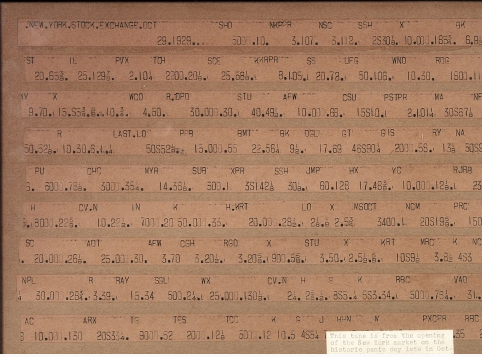
\includegraphics[width=\linewidth,height=0.4\textheight,keepaspectratio]{gfx/m3l3_notes_fig0_crash1929_ticker_tape.png}
\end{figure}

\emph{Khi các máy điện báo chứng khoán ghi lại giá cổ phiếu, mỗi giao dịch đều đi kèm một tiếng ``tích''.}

Nguồn: Museum of American Finance. ``Crash of 1929 Ticker Tape.'' \url{https://www.moaf.org/publications-collections/museum-collection/objects/crash-1929-ticker-tape}

``Dữ liệu tick'' được biết đến qua nhiều tên gọi, mỗi tên làm lộ ra một đặc điểm quan trọng của nó:

\begin{itemize}
  \item \textbf{Dữ liệu từng tick (tick-by-tick data)}: Mỗi điểm dữ liệu là một tick.
  \item \textbf{Dữ liệu tần suất (siêu) cao (High-Frequency data)}: Tần suất của các tick và khối lượng giao dịch rất cao, đặc biệt trong các thị trường có tính thanh khoản cao.
  \item \textbf{Giao dịch (Trades)}: Mỗi tick đại diện cho một giao dịch.
  \item \textbf{Giao dịch khớp lệnh (Transactions)}: Mỗi giao dịch là một giao dịch khớp giữa hai bên.
  \item \textbf{Dữ liệu thời gian thực (Real-time data)}: Dữ liệu này có thể được phân phối theo thời gian thực với độ trễ tối thiểu.
\end{itemize}

Dữ liệu tick không chỉ bao gồm dữ liệu giao dịch mà còn có thể bao gồm dữ liệu báo giá (quote). Dữ liệu này được gọi là sổ lệnh giới hạn (limit order book). Vì vậy, nếu một nhà tạo lập thị trường (market maker) tăng KHỐI LƯỢNG mà họ sẵn sàng mua và đặt một lệnh ở phía giá chào mua (bid), sẽ có thêm một quan sát làm thay đổi kích thước giá chào mua.

Tương tự, nếu một nhà tạo lập thị trường nâng giá chào mua (mức giá mà họ sẵn sàng mua), đó cũng sẽ là một quan sát bổ sung. Ngay cả khi không có giao dịch nào, dữ liệu sổ lệnh giới hạn vẫn là một nguồn thông tin phong phú chứa đựng ý định của những người tham gia. Như bạn sẽ thấy trong Hình 3.7, các ý định (giá chào mua mới, giá chào bán mới, hủy lệnh, v.v.) thay đổi nhanh hơn các hành động (các giao dịch thực tế) của những người tham gia.

Đến lúc này, có thể bạn đã có ít nhiều tiếp xúc với dữ liệu tài chính. Hầu hết mọi người đã từng thấy biểu đồ nến (candlestick) và biểu đồ giá với khoảng thời gian cố định trên trục $x$. Có những ứng dụng trực tuyến như TradingView hay Yahoo Finance và nhiều sàn giao dịch trực tuyến nơi người ta có thể vẽ đồ thị cổ phiếu mình chọn ở bất kỳ khoảng thời gian cố định nào và thậm chí dùng các chỉ báo yêu thích. Về bản chất, những gì bạn thấy là một tập dữ liệu có cấu trúc được tạo ra sau khi một số người hoặc đoạn mã chạy ngầm đã thu thập dữ liệu tick và tạo ra các thanh thời gian (time bar).

Mục đích của bài học này không chỉ là giới thiệu dữ liệu tick cho sinh viên, cho thấy dữ liệu trông như thế nào khi mới được tạo ra, mà còn hướng dẫn bạn tạo và vẽ các tập dữ liệu có cấu trúc mà bạn đã sử dụng từ trước đến nay. Nhờ vậy, chúng ta sẽ chuyển từ dữ liệu ở khâu sản xuất (dữ liệu tick) sang các tập dữ liệu sẵn sàng cho tiêu thụ, tương tự những tập sẽ được dùng trong các môn học sau cho mô hình hóa và phân tích.

Cần thấy rõ rằng dữ liệu tick (và hơn thế nữa là sổ lệnh tần suất cao) bao gồm dữ liệu chi tiết nhất mà bạn có thể tìm thấy. Nếu nghĩ hơi ngây thơ, người ta có thể nói rằng đây là toàn bộ dữ liệu được tạo ra khi giao dịch diễn ra, và do đó ta có thể kỳ vọng nó chứa mọi thông tin có thể có. Mặt khác, cũng có người có thể lập luận rằng còn nhiều yếu tố bên ngoài như xu hướng kinh tế vĩ mô, tâm lý thị trường, quy định pháp lý, tin tức, v.v. Tuy nhiên, nếu bạn tin vào giả thuyết thị trường hiệu quả, thì bạn nên kỳ vọng rằng bất kỳ yếu tố bên ngoài nào cũng sẽ được phản ánh vào giá ngay lập tức. Như vậy, thông tin bên ngoài trở thành một phần của giá và của dữ liệu giao dịch nói chung ngay khi nó được biết đến.

Vì dữ liệu tick có thể được phân phối theo thời gian thực, những nhà giao dịch phân tích dữ liệu này thay vì các thanh thời gian theo phút, giờ hoặc ngày (vốn lần lượt gộp thông tin trong một phút, một giờ hoặc một ngày) sẽ có thể trích xuất thông tin trước những người tham gia còn lại. Tuy nhiên, những nhà giao dịch này phải đối mặt với một nhiệm vụ rất khó: tách thông tin khỏi nhiễu.

\section{Các Ví dụ về Dữ liệu Tick}

Cho mục đích của bài học này, chúng tôi chọn ba tập dữ liệu tần suất cao khác nhau. Hai trong số đó gồm dữ liệu giao dịch từng tick, và tập thứ ba là dữ liệu Level 1 trộn với các giao dịch. Việc chọn các tài sản là ngẫu nhiên và chủ yếu bị ảnh hưởng bởi tính sẵn có của dữ liệu đó. Hầu như luôn luôn, dữ liệu tần suất cao không được cung cấp miễn phí mà khá đắt đỏ. Điều này là bình thường nếu xét đến lượng dữ liệu khổng lồ được tạo ra mỗi ngày và những khó khăn kỹ thuật trong việc lưu trữ và phân phối nó.

Vì lý do này, chúng ta sẽ khám phá:

1.) Các giao dịch từng tick BTC/USDT tải từ sàn Kraken: \url{https://support.kraken.com/hc/en-us/articles/360047543791-Downloadable-historical-market-data-time-and-sales-}

2.) Các giao dịch từng tick RVN/USDT tải từ sàn Binance: \url{https://data.binance.vision/}

3.) Dữ liệu Level 1 AGLJ/ZAR kèm các giao dịch, tải từ: \url{https://data.mendeley.com/datasets/4rrk89c3b2/2}

Do các hạn chế của máy ảo (VM), chỉ một phần rất nhỏ của dữ liệu trên được lấy mẫu cho mục đích giảng dạy. Nhưng bạn được khuyến khích tải các tập dữ liệu từng tick lớn về máy cục bộ để trực tiếp đối mặt với những khó khăn kỹ thuật khi xử lý dữ liệu lớn.

Dữ liệu giao dịch từng tick gồm các cột sau:

\begin{itemize}
  \item Symbol: mã định danh duy nhất của công cụ tài chính.
  \item Timestamp: thời điểm chính xác khi giao dịch được ghi nhận (độ chi tiết từ giây đến nano giây).
  \item Price: giá khớp của giao dịch.
  \item Volume: số đơn vị được giao dịch.
  \item Trade Direction (tùy chọn): cho biết giao dịch do bên mua hay bên bán khởi tạo.
\end{itemize}

Khía cạnh quan trọng nhất của dữ liệu tick, tức độ chi tiết (granularity), cho phép ta thực hiện:

\begin{itemize}
  \item Nghiên cứu độ biến động trong ngày.
  \item Hiểu quá trình hình thành giá một cách thấu đáo hơn.
  \item Kiểm định lùi (backtesting) các chiến lược giao dịch tần suất cao (HF).
  \item Đánh giá tác động thị trường để xác định việc mở rộng quy mô một chiến lược.
  \item Phân tích chi phí giao dịch của một chiến lược.
  \item Khám phá các chiến lược thực thi lệnh.
  \item Phát hiện thao túng thị trường (có thể được các cơ quan quản lý sử dụng).
  \item Tổng hợp thành các thanh theo thời gian hoặc theo khối lượng.
\end{itemize}

\begin{lstlisting}[language=Python,escapeinside={(*@}{@*)}]
import numpy as np
import pandas as pd
import matplotlib.pyplot as plt
import seaborn as sns
sns.set()
\end{lstlisting}

\begin{lstlisting}[language=Python,escapeinside={(*@}{@*)}]
# (*@Tải@*) (*@dữ@*) (*@liệu@*), (*@tập@*) (*@dữ@*) (*@liệu@*) (1) - BTC/USD (*@từ@*) Kraken
btc_usdt = pd.read_csv("XBTUSDT.csv", names=['UNIX_time', 'price', 'volume'])
btc_usdt.head()
\end{lstlisting}

\begin{lstlisting}[escapeinside={(*@}{@*)}]
    UNIX_time    price    volume
0  1688169604  30474.1  0.018800
1  1688169604  30474.8  0.000103
2  1688169604  30476.5  0.014997
3  1688169656  30483.5  0.000614
4  1688170008  30479.0  0.000328
\end{lstlisting}

Tập dữ liệu trên là một ví dụ về tập dữ liệu giao dịch từng tick, và nó gồm tất cả các giao dịch xảy ra trong một khoảng thời gian xác định. Điều đầu tiên bạn nhận thấy là cột UNIX\_time, nó không giống thời gian hay ngày tháng chút nào! Mốc thời gian này được gọi là ``thời gian UNIX'' (UNIX time), và nó đếm số đơn vị thời gian (giây, mili giây, micro giây và nano giây) tính từ 00:00:00 UTC ngày 1 tháng 1 năm 1970 cho đến nay.

Cách biểu diễn thời gian này mang lại:

\begin{itemize}
  \item Tính chuẩn hóa: biểu diễn thời gian phổ quát.
  \item Tính đơn giản: nó chỉ là một số nguyên duy nhất.
  \item Hiệu quả: các phép tính đơn giản và hiệu quả về mặt tính toán.
\end{itemize}

Các mốc thời gian Unix (Unix Timestamps) có thể được biểu diễn với các mức độ chính xác khác nhau:

\begin{itemize}
  \item 10 chữ số: Biểu diễn giây (ví dụ: 1688169604).
  \item 13 chữ số: Bao gồm mili giây (ví dụ: 1688169604123).
  \item 16 chữ số: Bao gồm micro giây (ví dụ: 1688169604123456).
  \item 19 chữ số: Bao gồm nano giây (ví dụ: 1688169604123456789).
\end{itemize}

Bạn cũng có thể xem trang web này: \url{https://unixtime.org/}.

Trong tập dữ liệu (1), ta đếm được 10 chữ số ở cột UNIX\_time. Do đó, độ chính xác được tính bằng giây, và đây là điều duy nhất ta cần biết để chuyển đổi thời gian Unix thành ngày giờ dễ đọc.

\begin{lstlisting}[language=Python,escapeinside={(*@}{@*)}]
# (*@Chuyển@*) (*@mốc@*) (*@thời@*) (*@gian@*) (*@UNIX@*) (*@thành@*) (*@ngày@*) (*@giờ@*) (*@dễ@*) (*@đọc@*). (*@Kiểm@*) (*@tra@*) (*@đối@*) (*@số@*) unit='s' (*@để@*) (*@đảm@*) (*@bảo@*) (*@mốc@*) (*@thời@*) (*@gian@*) (*@tính@*) (*@bằng@*) (*@giây@*).
btc_usdt['timestamp'] = pd.to_datetime(btc_usdt['UNIX_time'], unit='s')
btc_usdt.set_index('timestamp', inplace=True) # (*@Đặt@*) (*@timestamp@*) (*@làm@*) (*@chỉ@*) (*@mục@*)
btc_usdt.head()
\end{lstlisting}

\begin{lstlisting}[escapeinside={(*@}{@*)}]
                      UNIX_time    price    volume
timestamp                                         
2023-07-01 00:00:04  1688169604  30474.1  0.018800
2023-07-01 00:00:04  1688169604  30474.8  0.000103
2023-07-01 00:00:04  1688169604  30476.5  0.014997
2023-07-01 00:00:56  1688169656  30483.5  0.000614
2023-07-01 00:06:48  1688170008  30479.0  0.000328
\end{lstlisting}

\section{Trực quan hóa Dữ liệu Giao dịch Tick}

Bây giờ, hãy xem xét tập dữ liệu của chúng ta bằng hình ảnh. Việc trực quan hóa dữ liệu tick đặt ra những thách thức đặc thù do độ phân giải cực cao của nó. Hãy xét phép so sánh sau: hình dung bạn có một bức ảnh độ phân giải siêu cao được hiển thị trên một màn hình nhỏ hoặc được xem từ xa. Phần lớn chi tiết bị mất đi, và bạn có thể tự hỏi giá trị của độ phân giải cao như vậy là gì. Tương tự, khi vẽ dữ liệu tick, ta có nguy cơ che khuất các mẫu hình quan trọng nếu chỉ đơn giản vẽ mọi điểm. Mấu chốt là tìm những cách biểu diễn dữ liệu tần suất cao này sao cho làm lộ ra các mẫu hình và đặc điểm vốn có của nó mà không làm người xem bị choáng ngợp. Trong mục này, dữ liệu của chúng ta lấy từ ``TRTH JSE AGLJ.J Intraday Transaction Test Data'' của Gebbie và Nonyane và từ các tập dữ liệu được nhắc đến ở mục 2.

\begin{lstlisting}[language=Python,escapeinside={(*@}{@*)}]
#(*@Hình@*) 3.1
fig, ax = plt.subplots(figsize=(12, 5))
ax.scatter(btc_usdt.index, btc_usdt['price'], s = 0.001, alpha=0.4)
ax.set_ylabel('Price')
ax.set_title('BTC/USDT Price')
ax.set_ylim(20000, 32000)

custom_legend = plt.Line2D([0], [0], linestyle="none", marker='o', color='b', markersize=3, alpha = 0.7, label='Price') # (*@Tạo@*) (*@chú@*) (*@giải@*) (*@tùy@*) (*@chỉnh@*)
ax.legend(handles=[custom_legend], loc='upper right')

ax2 = ax.twinx() # (*@Tạo@*) (*@trục@*) (*@y@*) (*@thứ@*) (*@hai@*)
ax2.plot(btc_usdt.index, btc_usdt['volume'].rolling(10000).sum(), color='red', label='Volume: Rolling sum', alpha=0.3)
ax2.set_ylabel('Volume: Rolling sum')
ax2.set_ylim(200, 2300)

ax3 = ax.twinx() # (*@Tạo@*) (*@trục@*) (*@y@*) (*@thứ@*) (*@ba@*)
ax3.plot(btc_usdt.index, btc_usdt['volume'], color='purple', label='Volume', alpha=0.3)
ax3.set_ylabel('Volume')
ax3.set_ylim(0, 40)
ax3.spines['right'].set_position(('outward', 60))

fig.legend(bbox_to_anchor=(0.5,0.56)) # (*@Điều@*) (*@chỉnh@*) (*@vị@*) (*@trí@*) (*@chú@*) (*@giải@*)
plt.show()
\end{lstlisting}

\begin{figure}[H]
\centering
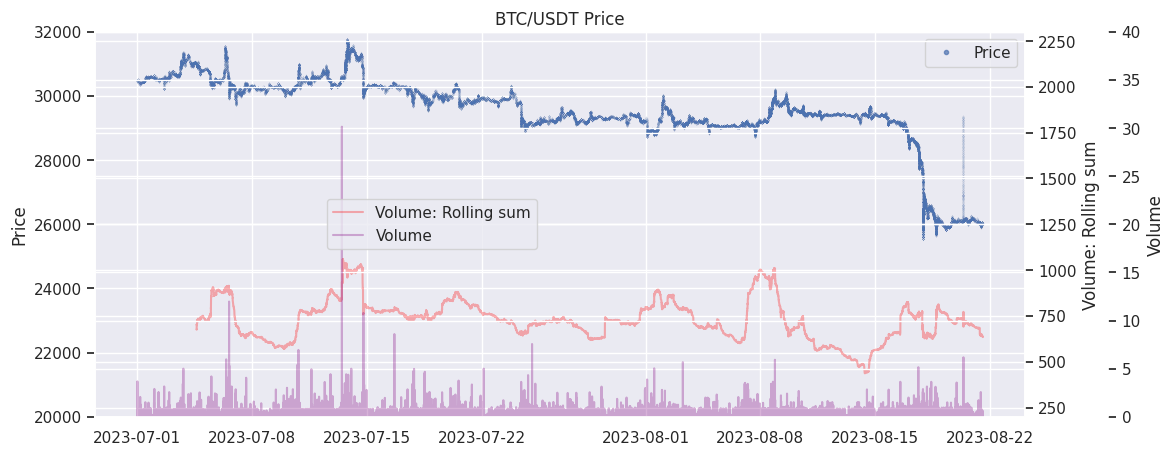
\includegraphics[width=\linewidth,height=0.6\textheight,keepaspectratio]{gfx/m3l3_notes_fig1_btcusdt_price_volume.png}
\par\smallskip{\small \textbf{Hình 3.1:} Giá BTC/USDT (biểu đồ phân tán) cùng khối lượng và tổng khối lượng trượt (rolling sum) trên các trục $y$ thứ hai và thứ ba}
\end{figure}

Cần lưu ý rằng các tập dữ liệu (1) và (2) được lấy trực tiếp từ các sàn giao dịch nơi chúng được tạo ra; do đó, ta kỳ vọng không có đầu vào bị thiếu. Điều đó không có nghĩa là dữ liệu không có lỗi!

Hãy khám phá tập dữ liệu của chúng ta:

\begin{lstlisting}[language=Python,escapeinside={(*@}{@*)}]
between_trades_interval = btc_usdt['UNIX_time'].diff().dropna() # (*@Tính@*) (*@thời@*) (*@lượng@*) (*@giữa@*) (*@các@*) (*@giao@*) (*@dịch@*)
print("Summary Statistics \n\n", between_trades_interval.describe(), "\n\n") # (*@Lấy@*) (*@thống@*) (*@kê@*) (*@tóm@*) (*@tắt@*) (*@của@*) (*@thời@*) (*@lượng@*) (*@giao@*) (*@dịch@*)
print("10 Largest trade durations \n\n", between_trades_interval.sort_values(ascending=False).head(10)) # (*@Lấy@*) 10 (*@khoảng@*) (*@thời@*) (*@gian@*) (*@lớn@*) (*@nhất@*) (*@giữa@*) (*@các@*) (*@giao@*) (*@dịch@*)
\end{lstlisting}

\begin{lstlisting}[escapeinside={(*@}{@*)}]
Summary Statistics 

 count    185042.000000
mean         24.072584
std          61.776399
min           0.000000
25%           0.000000
50%           0.000000
75%          18.000000
max        2195.000000
Name: UNIX_time, dtype: float64 


10 Largest trade durations 

 timestamp
2023-08-01 15:41:45    2195.0
2023-07-12 09:19:13    2001.0
2023-08-17 10:30:32    1809.0
2023-08-18 15:05:14    1576.0
2023-07-23 07:29:23    1281.0
2023-07-23 02:13:51    1244.0
2023-08-06 03:40:46    1224.0
2023-07-20 23:44:23    1125.0
2023-07-16 03:52:08    1113.0
2023-07-19 05:28:45    1100.0
Name: UNIX_time, dtype: float64
\end{lstlisting}

Xét từ các kết quả trên (thời lượng giao dịch cao), cặp BTC/USDT trong mẫu cụ thể này có vẻ kém thanh khoản. Nhưng ta biết rằng tính thanh khoản có thể thay đổi rất lớn theo thời gian và mẫu này có thể không đại diện cho tính thanh khoản của cặp này trên sàn này. Để rút ra kết luận vững chắc hơn, ta cần phân tích một tập dữ liệu lớn hơn, trải dài qua các giai đoạn và điều kiện thị trường khác nhau.

Hãy kiểm tra phân phối của khối lượng, lợi suất đơn giản và các khoảng thời gian giữa các giao dịch.

\begin{lstlisting}[language=Python,escapeinside={(*@}{@*)}]
#(*@Hình@*) 3.2
fig, (ax1, ax2, ax3) = plt.subplots(1, 3, figsize=(15, 4))
ax1.hist(between_trades_interval, bins=100, color='skyblue', edgecolor='black', linewidth=1.2)
ax1.set_title("Time between trades")
ax2.hist(btc_usdt['price'].pct_change().dropna(), bins=100, color='white', edgecolor='black', linewidth=1.2)
ax2.set_title("Simple Returns")
ax3.hist(btc_usdt['volume'], bins=100, color='green', edgecolor='black', linewidth=1.2)
ax3.set_title("Volume")
plt.show()
\end{lstlisting}

\begin{figure}[H]
\centering
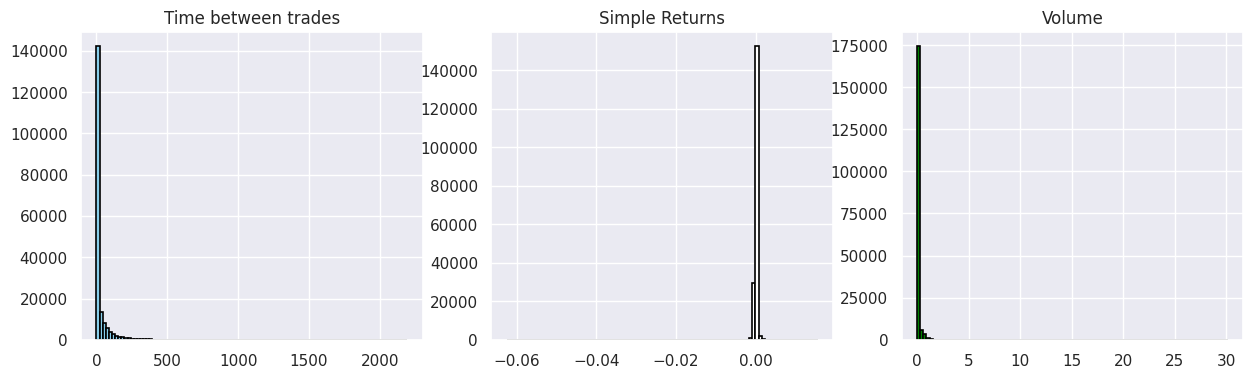
\includegraphics[width=\linewidth,height=0.6\textheight,keepaspectratio]{gfx/m3l3_notes_fig2_raw_tick_histograms.png}
\par\smallskip{\small \textbf{Hình 3.2:} Histogram của thời gian giữa các giao dịch, lợi suất đơn giản và khối lượng của dữ liệu tick BTC/USDT gốc}
\end{figure}

Các kết quả trên gợi ý ba sự thật quan trọng:

\begin{itemize}
  \item Có nhiều giao dịch xảy ra trong cùng một giây. Những giao dịch này có thể là một giao dịch duy nhất bị chia thành nhiều giao dịch tại thời điểm thực thi do khối lượng ở mức giá chào mua hoặc giá chào bán tốt nhất không đủ để đáp ứng khối lượng giao dịch tại thời điểm đó. Những giao dịch này được gọi là \textbf{giao dịch bị chia nhỏ (split transactions)}.
  \item Có nhiều giao dịch không làm giá thay đổi.
  \item Rất nhiều giao dịch dường như có khối lượng rất thấp.
\end{itemize}

\begin{lstlisting}[language=Python,escapeinside={(*@}{@*)}]
boolean_array_is_duplicate = btc_usdt['UNIX_time'].duplicated(keep=False) # (*@Kiểm@*) (*@tra@*) (*@các@*) (*@bản@*) (*@trùng@*) (*@lặp@*)
sum_of_duplicates = boolean_array_is_duplicate.sum() # (*@Tính@*) (*@tổng@*) (*@các@*) (*@bản@*) (*@trùng@*) (*@lặp@*)
print("The number of trades that occured at the same second with at least one more trade, is: ",sum_of_duplicates)
print("The percentage of these trades to the number of all trades, is: ",round(sum_of_duplicates / len(btc_usdt) * 100, 2), "%")
print("The percentage of the volume of these trades to the entire volume, is: ",round(((boolean_array_is_duplicate * btc_usdt['volume']).sum() / btc_usdt['volume'].sum() )* 100, 2), "%")
\end{lstlisting}

\begin{lstlisting}[escapeinside={(*@}{@*)}]
The number of trades that occured at the same second with at least one more trade, is:  126239
The percentage of these trades to the number of all trades, is:  68.22 %
The percentage of the volume of these trades to the entire volume, is:  91.13 %
\end{lstlisting}

Chúng ta sẽ giả định rằng những giao dịch này là các giao dịch bị chia nhỏ. Sau một vài phép tổng hợp đơn giản, các histogram vẽ ở trên trông rất khác:

\begin{lstlisting}[language=Python,escapeinside={(*@}{@*)}]
# (*@Hình@*) 3.3
aggr_dataset_1 = pd.DataFrame()
aggr_dataset_1['UNIX_time'] = btc_usdt['UNIX_time'].groupby(btc_usdt['UNIX_time']).first() # (*@Nhóm@*) (*@mốc@*) (*@thời@*) (*@gian@*) (*@UNIX@*) (*@theo@*) (*@mốc@*) (*@thời@*) (*@gian@*) (*@đầu@*) (*@tiên@*)
aggr_dataset_1['volume'] = btc_usdt['volume'].groupby(btc_usdt['UNIX_time']).sum() # (*@Tổng@*) (*@hợp@*) (*@khối@*) (*@lượng@*) (*@theo@*) (*@mốc@*) (*@thời@*) (*@gian@*) (*@UNIX@*)
aggr_dataset_1['price'] = (btc_usdt['price'] * btc_usdt['volume']).groupby(btc_usdt['UNIX_time']).sum() / aggr_dataset_1['volume'] # (*@Giá@*) (*@cuối@*) (*@cùng@*) (*@là@*) VWAP (*@của@*) (*@giao@*) (*@dịch@*) (*@bị@*) (*@chia@*) (*@nhỏ@*)
aggr_dataset_1.index = btc_usdt.index.drop_duplicates() # (*@Loại@*) (*@bỏ@*) (*@các@*) (*@bản@*) (*@trùng@*) (*@lặp@*) (*@khỏi@*) (*@chỉ@*) (*@mục@*)

fig, (ax1, ax2, ax3) = plt.subplots(1, 3, figsize=(15, 4))
ax1.hist(aggr_dataset_1['UNIX_time'].diff().dropna(), bins=100, color='skyblue', edgecolor='black', linewidth=1.2)
ax1.set_title("Time between trades")
ax2.hist(aggr_dataset_1['price'].pct_change().dropna(),bins=100, color='white', edgecolor='black', linewidth=1.2)
ax2.set_title("Simple Returns")
ax3.hist(aggr_dataset_1['volume'], bins=100, color='green', edgecolor='black', linewidth=1.2)
ax3.set_title("Volume")
plt.show()
\end{lstlisting}

\begin{lstlisting}[escapeinside={(*@}{@*)}]
/tmp/ipykernel_45/2642210345.py:11: FutureWarning: The default fill_method='pad' in Series.pct_change is deprecated and will be removed in a future version. Either fill in any non-leading NA values prior to calling pct_change or specify 'fill_method=None' to not fill NA values.
  ax2.hist(aggr_dataset_1['price'].pct_change().dropna(),bins=100, color='white', edgecolor='black', linewidth=1.2)
\end{lstlisting}

\begin{figure}[H]
\centering
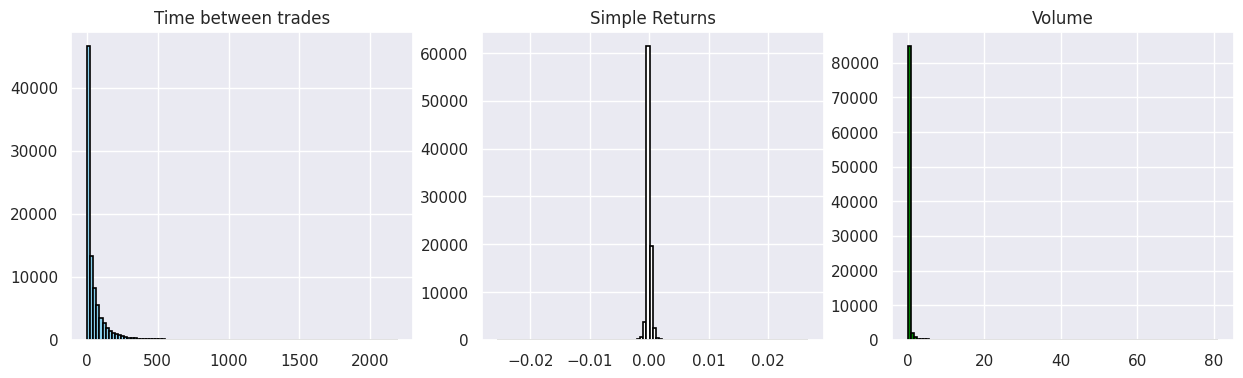
\includegraphics[width=\linewidth,height=0.6\textheight,keepaspectratio]{gfx/m3l3_notes_fig3_aggregated_histograms.png}
\par\smallskip{\small \textbf{Hình 3.3:} Histogram của thời gian giữa các giao dịch, lợi suất đơn giản và khối lượng sau khi tổng hợp các giao dịch bị chia nhỏ}
\end{figure}

Tại thời điểm này, ta có thể tiếp tục quy trình bằng phân tích lợi suất, mất cân bằng dòng lệnh (order flow imbalance, OFI), ước lượng độ biến động, thước đo thanh khoản, v.v. Vì các tập dữ liệu này sẽ được dùng để trình bày dữ liệu tick chứ không phải để phân tích, chúng ta sẽ chuyển sang tập dữ liệu (2), và một quy trình giới thiệu sẽ được trình bày với tập dữ liệu (3).

\section{Bao gồm Hướng Giao dịch}

Hãy xem tập dữ liệu (2), chứa các giao dịch RVN/USDT nhưng có thêm một điều so với tập dữ liệu (1): có một cột bổ sung, ``Trade Direction'', chứa thông tin cho biết nhà giao dịch khởi tạo giao dịch là bên mua hay bên bán. Trong trường hợp của chúng ta, sàn giao dịch lưu một giá trị boolean (True, False) cho mỗi dòng, trả lời câu hỏi \emph{bên mua có phải là nhà tạo lập thị trường (market maker) hay không?}

Như ta biết, mỗi giao dịch phải có một bên mua và một bên bán. Nếu câu trả lời cho câu hỏi trên là đúng (true), thì nhà tạo lập thị trường đã đặt một lệnh chào mua (bid) vào sổ lệnh với ý định mua, và một bên bán đã khởi tạo giao dịch bằng cách khớp (một phần?) lệnh mua đó. Ngược lại, nếu câu trả lời là sai (false), thì nhà tạo lập thị trường là bên bán đã đặt một lệnh chào bán (ask). Trong trường hợp này, bên khởi tạo giao dịch là một bên mua đã khớp lệnh chào bán cụ thể đó.

Mảng boolean bổ sung này là một nguồn thông tin có giá trị.

Chúng ta sẽ bắt đầu bằng việc tải tập dữ liệu (2). Trong nhiều trường hợp, nhà cung cấp dữ liệu hoặc sàn giao dịch sẽ cho phép bạn tải dữ liệu dưới dạng các tệp \texttt{csv}, mỗi tệp chứa dữ liệu của một ngày (hoặc một tuần, hoặc một tháng, hoặc một khoảng thời gian tùy chỉnh). Trong trường hợp của chúng ta, tập dữ liệu (2) gồm bốn tệp theo ngày. Chúng ta sẽ dùng thư viện \texttt{glob} vì sự đơn giản của nó trong việc chọn các tệp cần thiết: \url{https://builtin.com/software-engineering-perspectives/glob-in-python}.

\begin{lstlisting}[language=Python,escapeinside={(*@}{@*)}]
import glob

# (*@Tải@*) (*@dữ@*) (*@liệu@*), (*@tập@*) (*@dữ@*) (*@liệu@*) (2) - RVN/USDT
list_of_files = glob.glob('RVNUSDT*') # (*@Liệt@*) (*@kê@*) (*@các@*) (*@tệp@*) RVNUSDT (*@trong@*) (*@thư@*) (*@mục@*)
column_names = ['id', 'price', 'qty', 'base_qty', 'UNIX_time', 'is_buyer_maker', 'is_best_match'] # (*@Tên@*) (*@các@*) (*@cột@*)
rvn_usdt = pd.concat([pd.read_csv(file, names=column_names) for file in list_of_files], ignore_index=True, axis = 0) # (*@Nối@*) (*@các@*) (*@tệp@*)
rvn_usdt.sort_values('UNIX_time', inplace=True) # (*@Sắp@*) (*@xếp@*) (*@các@*) (*@giá@*) (*@trị@*) (*@theo@*) (*@thời@*) (*@gian@*)
rvn_usdt.head(5)
\end{lstlisting}

\begin{lstlisting}[escapeinside={(*@}{@*)}]
              id    price      qty    base_qty     UNIX_time is_buyer_maker  \
148005  55947315  0.02103  10000.0  210.300000  1.688100e+04            NaN   
148006  54407520  0.02588    424.9   10.996412  1.680307e+12          False   
148007  54407521  0.02588   3313.5   85.753380  1.680307e+12          False   
148008  54407522  0.02588   4172.5  107.984300  1.680307e+12          False   
148011  54407525  0.02589   1105.3   28.616217  1.680307e+12          False   

       is_best_match  
148005           NaN  
148006          True  
148007          True  
148008          True  
148011          True  
\end{lstlisting}

Hãy lùi lại một chút. Tập dữ liệu (2) là một tập dữ liệu giao dịch từng tick, nhưng có số cột gấp đôi so với tập dữ liệu (1). Đến đây cần thấy rõ rằng, tùy nhà cung cấp dữ liệu và/hoặc sàn giao dịch, có thể có thêm các cột ngoài ba cột cơ bản (giá, khối lượng và mốc thời gian). Trong trường hợp của chúng ta, phần bổ sung có ý nghĩa duy nhất so với các cột cơ bản là cột \texttt{is\_buyer\_maker}.

Cột \texttt{base\_qty} biểu diễn khối lượng của tiền tệ cơ sở (loại tiền tệ mà tài sản được giao dịch đối ứng) được giao dịch, cho trước khối lượng tài sản được giao dịch và giá của giao dịch: $\text{base\_qty} = \text{qty} \cdot \text{price}$. Cột \texttt{id} biểu diễn mã định danh của từng giao dịch và có thể dùng để lọc các bản ghi trùng lặp. Cuối cùng, cột \texttt{is\_best\_match} là một mảng boolean cho biết giao dịch có được thực thi tại mức giá tốt nhất có thể, xét theo sổ lệnh tại thời điểm đó, hay không (True hoặc False).

Chúng ta sẽ kiểm tra xem các cột bổ sung có chứa thông tin nào không trước khi loại bỏ chúng để xử lý một tập dữ liệu nhỏ hơn, giúp giảm tải cho bộ nhớ RAM.

\begin{lstlisting}[language=Python,escapeinside={(*@}{@*)}]
print("Number of duplicate entries: ", rvn_usdt['id'].duplicated().sum()) # (*@Kiểm@*) (*@tra@*) (*@các@*) (*@bản@*) (*@trùng@*) (*@lặp@*)
print("Number of entries that were not executed at the best possible price: ",  (~(rvn_usdt['is_best_match'].astype("bool"))).sum()) # (*@Kiểm@*) (*@tra@*) (*@khớp@*) (*@tốt@*) (*@nhất@*)
print("Can the base_qty be derived from the qty and price?: ", np.isclose(rvn_usdt['price'] * rvn_usdt['qty'], rvn_usdt['base_qty'], atol=1e-05).all()) # (*@Kiểm@*) (*@tra@*) (*@xem@*) (*@lượng@*) (*@cơ@*) (*@sở@*) (*@có@*) (*@thể@*) (*@suy@*) (*@ra@*) (*@từ@*) (*@lượng@*) (*@giao@*) (*@dịch@*) (*@hay@*) (*@không@*)
print("Due to the results above, we can drop the columns 'id', 'is_best_match' and 'base_qty' \n\n")

rvn_usdt = rvn_usdt.drop(columns=['id', 'is_best_match', 'base_qty']) # (*@Loại@*) (*@bỏ@*) (*@các@*) (*@cột@*) (*@không@*) (*@cần@*) (*@thiết@*)
rvn_usdt['timestamp'] = pd.to_datetime(rvn_usdt['UNIX_time'], unit='ms') # (*@Chuyển@*) (*@mốc@*) (*@thời@*) (*@gian@*) (*@UNIX@*) (*@thành@*) (*@ngày@*) (*@giờ@*) (*@dễ@*) (*@đọc@*). (*@Kiểm@*) (*@tra@*) (*@đối@*) (*@số@*) unit='ms' (*@để@*) (*@đảm@*) (*@bảo@*) (*@mốc@*) (*@thời@*) (*@gian@*) (*@tính@*) (*@bằng@*) (*@mili@*) (*@giây@*).
rvn_usdt.set_index('timestamp', inplace=True) # (*@Đặt@*) (*@timestamp@*) (*@làm@*) (*@chỉ@*) (*@mục@*)
rvn_usdt.head()
\end{lstlisting}

\begin{lstlisting}[escapeinside={(*@}{@*)}]
Number of duplicate entries:  0
Number of entries that were not executed at the best possible price:  0
Can the base_qty be derived from the qty and price?:  False
Due to the results above, we can drop the columns 'id', 'is_best_match' and 'base_qty' 



                           price      qty     UNIX_time is_buyer_maker
timestamp                                                             
1970-01-01 00:00:16.881  0.02103  10000.0  1.688100e+04            NaN
2023-04-01 00:00:15.745  0.02588    424.9  1.680307e+12          False
2023-04-01 00:00:15.759  0.02588   3313.5  1.680307e+12          False
2023-04-01 00:00:15.759  0.02588   4172.5  1.680307e+12          False
2023-04-01 00:00:15.762  0.02589   1105.3  1.680307e+12          False
\end{lstlisting}

\section{Xử lý Dữ liệu Tick}

Từ đây trở đi, khi nói ``khối lượng mua'' (buying volume) hay ``khối lượng bán'' (selling volume), chúng ta sẽ chỉ khối lượng của các giao dịch mà bên khởi tạo/bên nhận lệnh (taker) lần lượt là bên mua hoặc bên bán. Để hiểu cách sử dụng thông tin bổ sung này, chúng ta sẽ trình bày các thao tác xử lý dữ liệu thiết yếu để tính khối lượng mua và khối lượng bán.

\begin{lstlisting}[language=Python,escapeinside={(*@}{@*)}]
# (*@Hình@*) 3.4
buying_volume = rvn_usdt['qty'] * (~(rvn_usdt['is_buyer_maker'].astype("bool"))) # (*@Một@*) (*@mảng@*) (*@chứa@*) (*@khối@*) (*@lượng@*) (*@mua@*)
selling_volume = rvn_usdt['qty'] * rvn_usdt['is_buyer_maker'].astype("bool") # (*@Một@*) (*@mảng@*) (*@chứa@*) (*@khối@*) (*@lượng@*) (*@bán@*)

print("The buying volume is: ", buying_volume.sum()) # (*@Tính@*) (*@khối@*) (*@lượng@*) (*@mua@*)
print("The selling volume is: ", selling_volume.sum()) # (*@Tính@*) (*@khối@*) (*@lượng@*) (*@bán@*)

fig, (ax1, ax2) = plt.subplots(1, 2, figsize=(15, 4))
ax1.hist(buying_volume, log = True, bins=100, color='skyblue', edgecolor='black', linewidth=1.2)
ax1.set_title("Buying Volume")
ax2.hist(selling_volume, log = True, bins=100, color='green', edgecolor='black', linewidth=1.2)
ax2.set_title("Selling Volume")
plt.show()
\end{lstlisting}

\begin{lstlisting}[escapeinside={(*@}{@*)}]
The buying volume is:  658280433.4000001
The selling volume is:  684682634.6999999
\end{lstlisting}

\begin{figure}[H]
\centering
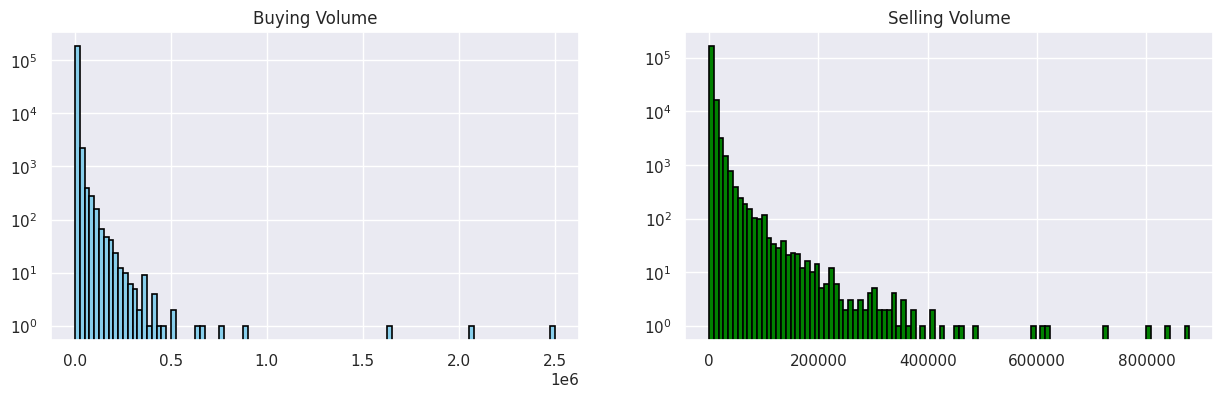
\includegraphics[width=\linewidth,height=0.6\textheight,keepaspectratio]{gfx/m3l3_notes_fig4_buying_selling_volume.png}
\par\smallskip{\small \textbf{Hình 3.4:} Histogram (trục $y$ theo thang log) của khối lượng mua và khối lượng bán của RVN/USDT}
\end{figure}

\textbf{Bài tập 1}

Trong histogram ở trên, chúng ta đã dùng đối số \texttt{log = True} để chuyển trục $y$ sang thang log. Để hiểu vì sao, hãy vẽ các histogram của khối lượng mua và khối lượng bán với \texttt{log = False}. Hơn nữa, hãy phân biệt giữa việc biến đổi trục $y$ cho mục đích trực quan hóa và việc biến đổi chính dữ liệu bằng logarit tự nhiên. Hãy tạo lại hai histogram với \texttt{log = False}, nhưng dùng hàm \texttt{np.log} để biến đổi khối lượng mua và khối lượng bán: \texttt{np.log(buying\_volume[buying\_volume > 1])}. Làm tương tự với các histogram trình bày trong Hình 3.3. Hãy giải thích các khác biệt.

\textbf{Bài tập 2}

Tính kích thước tick (tick size) cho các tập dữ liệu (1) và (2). Hãy giải thích phương pháp của bạn trên diễn đàn.

Bây giờ chúng ta sẽ vẽ khối lượng mua và khối lượng bán theo cách trực quan bắt mắt. Khi vẽ dữ liệu độ phân giải cao, việc thu nhỏ để xem ``bức tranh toàn cảnh'' là vô nghĩa. Ngược lại, chúng ta chọn các đồ thị phóng to hoặc các đồ thị tương tác (plotly, bokeh) nơi ta có thể phóng to theo yêu cầu.

\begin{lstlisting}[language=Python,escapeinside={(*@}{@*)}]
# (*@Hình@*) 3.5
start = rvn_usdt.index[rvn_usdt.index >= "2023-07-01 01:53:15.745"][0]
end   = rvn_usdt.index[rvn_usdt.index <= "2023-07-01 01:54:15.745"][-1]

rvn_usdt_slice = rvn_usdt.loc[start:end] # (*@Cắt@*) (*@lát@*) (*@dữ@*) (*@liệu@*)

fig, ax = plt.subplots(figsize=(15, 5))

ax.scatter(x = rvn_usdt_slice[rvn_usdt_slice['is_buyer_maker'] == True].index, \
           y = rvn_usdt_slice[rvn_usdt_slice['is_buyer_maker'] == True]['price'], color='red', \
            label='Buyer Maker / Seller Taker', alpha = 0.4) # (*@Vẽ@*) (*@giao@*) (*@dịch@*) (*@bên@*) (*@mua@*) (*@tạo@*) (*@lập@*) / (*@bên@*) (*@bán@*) (*@nhận@*) (*@lệnh@*)
ax.scatter(x = rvn_usdt_slice[rvn_usdt_slice['is_buyer_maker'] == False].index, \
           y = rvn_usdt_slice[rvn_usdt_slice['is_buyer_maker'] == False]['price'], color='green', \
            label='Seller Maker / Buyer Taker', alpha = 0.4) # (*@Vẽ@*) (*@giao@*) (*@dịch@*) (*@bên@*) (*@bán@*) (*@tạo@*) (*@lập@*) / (*@bên@*) (*@mua@*) (*@nhận@*) (*@lệnh@*)
ax.set_title("RVN/USDT buyers/sellers trades")
ax.set_xlabel("Time")
ax.set_ylabel("Price")
ax.legend()
plt.show()
\end{lstlisting}

\begin{figure}[H]
\centering
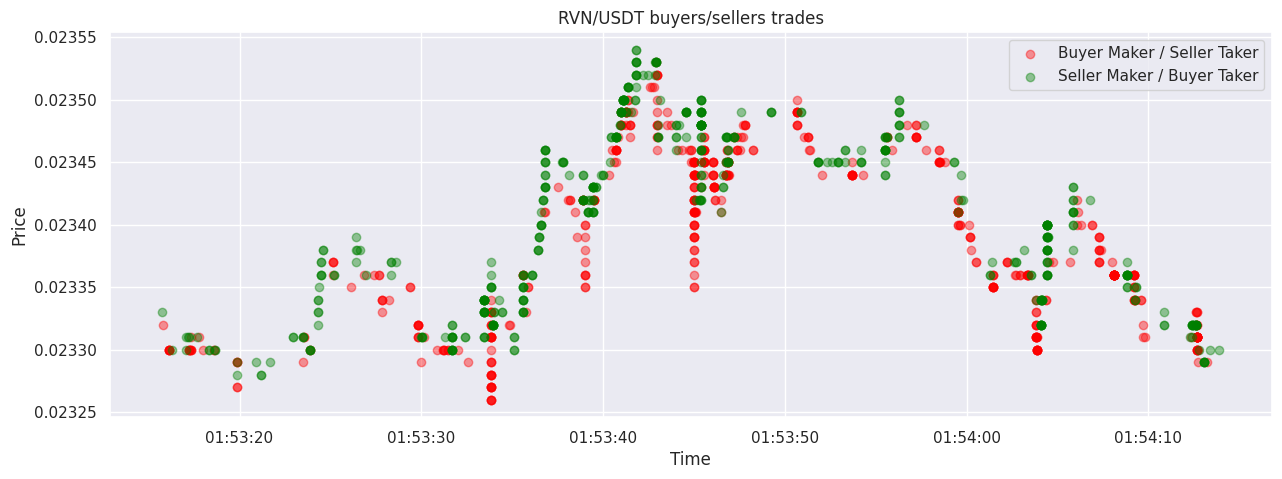
\includegraphics[width=\linewidth,height=0.6\textheight,keepaspectratio]{gfx/m3l3_notes_fig5_buyer_seller_scatter.png}
\par\smallskip{\small \textbf{Hình 3.5:} Biểu đồ phân tán giá các giao dịch RVN/USDT trong khoảng một phút, phân biệt bên mua tạo lập/bên bán nhận lệnh (đỏ) và bên bán tạo lập/bên mua nhận lệnh (xanh lá)}
\end{figure}

\textbf{Bài tập 3}

Trong Hình 3.5, ta thấy một đồ thị phóng to các giao dịch của bên mua và bên bán của RVN/USDT. Khoảng thời gian được chọn chính xác là 1 phút. Trong bài tập này, bạn phải tạo lại Hình 3.5 cho các khoảng thời gian khác nhau. Bạn có thể chọn các khoảng dài hơn và/hoặc các thời điểm khác nhau. Để có một hướng dẫn trong việc chọn các khoảng thời gian mà bạn \textbf{quan tâm}, bạn sẽ phải vẽ toàn bộ đồ thị giá của cặp RVN/USDT.

\textbf{Bài tập 4} \emph{(Tùy chọn)}

Dùng mã được cung cấp trong notebook này làm hướng dẫn, hãy tải dữ liệu tick về máy cục bộ để tiếp tục quy trình làm việc trên máy tính của riêng bạn. Sau đó, hãy thử dùng plotly hoặc bokeh (holoviews) để tạo các đồ thị tương tác cho phép bạn phóng to mà không phải cắt lát tập dữ liệu mỗi khi muốn tạo một đồ thị mới. Xem thư viện đồ thị do plotly cung cấp tại \url{https://plotly.com/python/}, và đảm bảo bạn hiểu sự khác biệt giữa đồ thị tương tác và đồ thị tĩnh.

\section{Dữ liệu Cấp 1 (Level 1, L1)}

Dữ liệu Level 1 (hay còn gọi là dữ liệu đỉnh sổ lệnh, top-of-book data, TOB) thường bao gồm các cột sau:

\begin{itemize}
  \item Symbol: mã định danh duy nhất của công cụ tài chính.
  \item Timestamp: thời điểm chính xác khi sự kiện được ghi nhận.
  \item Bid price: mức giá cao nhất mà một bên mua sẵn sàng trả.
  \item Ask price: mức giá thấp nhất mà một bên bán sẵn sàng chấp nhận.
  \item Ask volume (khối lượng chào bán): số đơn vị có sẵn tại mức giá chào bán.
  \item Bid Volume (khối lượng chào mua): số đơn vị có sẵn tại mức giá chào mua.
\end{itemize}

\begin{lstlisting}[language=Python,escapeinside={(*@}{@*)}]
# (*@Tải@*) (*@dữ@*) (*@liệu@*), (*@tập@*) (*@dữ@*) (*@liệu@*) (3) - AGLJ_J
columns = ['RIC', 'DateTimeL', 'Type', 'Price', 'Volume', 'L1 Bid', 'L1 Ask', 'Trade Sign']
aglj = pd.read_csv('AGLJ_J_04-Jan-2016_TO_10-May-2016_5days.csv', \
                   names = columns, skiprows = 1) # (*@Tải@*) (*@dữ@*) (*@liệu@*)
aglj.sort_values(by = 'DateTimeL', inplace = True)
aglj.head(5)
\end{lstlisting}

\begin{lstlisting}[escapeinside={(*@}{@*)}]
       RIC      DateTimeL    Type   Price  Volume  L1 Bid  L1 Ask  Trade Sign
0   AGLJ.J  736333.382013   Trade  6750.0   366.0     0.0     0.0         0.0
1   AGLJ.J  736333.382013   Quote     0.0     0.0     0.0  6800.0         0.0
2   AGLJ.J  736333.382015   Trade  6750.0   374.0     0.0     0.0         0.0
3   AGLJ.J  736333.382015   Quote     0.0     0.0     0.0  6800.0         0.0
4   AGLJ.J  736333.382015   Quote     0.0     0.0  6735.0  6800.0         0.0
\end{lstlisting}

Điều đầu tiên cần chú ý là cột \texttt{DateTimeL}. Đây là một định dạng khác mà bạn có thể gặp khi dùng dữ liệu tick, và nó biểu diễn một số \emph{ngày tuần tự (serial date)} thể hiện ngày và giờ. Cụ thể, nó đếm số ngày tính từ một ngày cho trước, gọi là \texttt{base\_date}. Trong trường hợp của chúng ta, \texttt{base\_date} là ngày 1 tháng 1 năm 0000. Ví dụ, 736333.382013 được hiểu là ngày thứ 736333 kể từ ngày 1 tháng 1 năm 0000. Phần thập phân biểu diễn phần của ngày. Trong ví dụ của chúng ta, ngày thứ 736333 là ngày 4 tháng 1 năm 2016, và phần 0.382013 tương ứng với 09:10:05.

Với sự trợ giúp của thư viện Python \texttt{datetime}, chúng ta sẽ chuyển ngày tuần tự thành dạng dễ đọc. Nhưng việc này không phải không có vấn đề! Lịch của thư viện \texttt{datetime} bắt đầu từ ngày 1 tháng 1 năm 0001, vì về mặt lịch sử không có năm 0000. Mặt khác, việc đánh chỉ số từ 0 được ưu tiên trong các tính toán khoa học. Sinh viên không cần đi sâu vào vấn đề này, nhưng đây là một ví dụ tốt về các cách ký hiệu khác nhau mà người ta gặp phải khi xử lý dữ liệu tick.

\begin{lstlisting}[language=Python,escapeinside={(*@}{@*)}]
from datetime import datetime, timedelta

def convert_serial_to_datetime(serial):
    # (*@Xác@*) (*@định@*) (*@ngày@*) (*@cơ@*) (*@sở@*) (*@là@*) (*@ngày@*) 1 (*@tháng@*) 1 (*@năm@*) 0001
    base_date = datetime(1, 1, 1)

    # (*@Tách@*) (*@ngày@*) (*@tuần@*) (*@tự@*) (*@thành@*) (*@số@*) (*@ngày@*) (*@và@*) (*@phần@*) (*@lẻ@*) (*@của@*) (*@ngày@*)
    days = int(serial)
    fractional_day = serial - days

    # (*@Điều@*) (*@chỉnh@*) (*@do@*) (*@không@*) (*@có@*) (*@năm@*) 0 (*@bằng@*) (*@cách@*) (*@trừ@*) (*@đi@*) 367 (*@ngày@*)
    adjusted_days = days - 367

    # (*@Tính@*) (*@ngày@*) (*@đích@*) (*@bằng@*) (*@cách@*) (*@cộng@*) (*@số@*) (*@ngày@*) (*@đã@*) (*@điều@*) (*@chỉnh@*) (*@và@*) (*@phần@*) (*@lẻ@*) (*@của@*) (*@ngày@*) ((*@quy@*) (*@đổi@*) (*@ra@*) (*@giây@*)) (*@vào@*) (*@ngày@*) (*@cơ@*) (*@sở@*)
    target_date = base_date + timedelta(days=adjusted_days) + timedelta(seconds=fractional_day * 86400)

    # (*@Trả@*) (*@về@*) (*@ngày@*) (*@đích@*) (*@ở@*) (*@định@*) (*@dạng@*) (*@dễ@*) (*@đọc@*)
    return target_date.strftime('%Y-%m-%d %H:%M:%S')

aglj['timestamp'] = aglj['DateTimeL'].apply(convert_serial_to_datetime) # (*@Chuyển@*) (*@ngày@*) (*@tuần@*) (*@tự@*) (*@thành@*) (*@ngày@*) (*@giờ@*) (*@dễ@*) (*@đọc@*)
aglj['timestamp'] = pd.to_datetime(aglj['timestamp']) # (*@Chuyển@*) (*@mốc@*) (*@thời@*) (*@gian@*) (*@thành@*) (*@đối@*) (*@tượng@*) (*@datetime@*)
aglj.set_index('timestamp', inplace=True) # (*@Đặt@*) (*@timestamp@*) (*@làm@*) (*@chỉ@*) (*@mục@*)
aglj.head(5)
\end{lstlisting}

\begin{lstlisting}[escapeinside={(*@}{@*)}]
                         RIC      DateTimeL    Type   Price  Volume  L1 Bid  \
timestamp                                                                     
2016-01-04 09:10:05   AGLJ.J  736333.382013   Trade  6750.0   366.0     0.0   
2016-01-04 09:10:05   AGLJ.J  736333.382013   Quote     0.0     0.0     0.0   
2016-01-04 09:10:06   AGLJ.J  736333.382015   Trade  6750.0   374.0     0.0   
2016-01-04 09:10:06   AGLJ.J  736333.382015   Quote     0.0     0.0     0.0   
2016-01-04 09:10:06   AGLJ.J  736333.382015   Quote     0.0     0.0  6735.0   

                     L1 Ask  Trade Sign  
timestamp                                
2016-01-04 09:10:05     0.0         0.0  
2016-01-04 09:10:05  6800.0         0.0  
2016-01-04 09:10:06     0.0         0.0  
2016-01-04 09:10:06  6800.0         0.0  
2016-01-04 09:10:06  6800.0         0.0  
\end{lstlisting}

Bây giờ hãy áp dụng một số bộ lọc làm sạch:

Trước khi có thể phân tích hiệu quả dữ liệu tài chính tần suất cao, điều thiết yếu là làm sạch và tiền xử lý tập dữ liệu. Quá trình làm sạch này giúp loại bỏ các bản ghi sai sót và điều chỉnh một số hiệu ứng vi cấu trúc thị trường, đảm bảo rằng các phân tích sau đó dựa trên dữ liệu chính xác và có ý nghĩa.

Trước hết, chúng ta loại bỏ các bản ghi có giá, báo giá hoặc khối lượng bằng không hoặc âm. Đây nhiều khả năng là lỗi dữ liệu, vì giá và khối lượng trong các thị trường tài chính luôn phải dương. Các chênh lệch âm (negative spread), tức khi giá chào mua vượt giá chào bán, cũng bị loại bỏ vì chúng biểu diễn các điều kiện thị trường bất khả thi trong hoàn cảnh bình thường.

Tiếp theo, chúng ta giải quyết vấn đề giao dịch bị chia nhỏ. Trong giao dịch tần suất cao, một lệnh lớn duy nhất có thể được thực thi thành nhiều giao dịch nhỏ hơn tại cùng một mốc thời gian. Điều này có thể dẫn đến việc biểu diễn quá mức một số mức giá và có khả năng làm lệch phân tích của chúng ta. Để giảm thiểu điều này, chúng ta gộp các giao dịch xảy ra tại cùng một mốc thời gian, cộng khối lượng của chúng và tính giá trung bình theo khối lượng (VWAP). Cách tiếp cận này bảo toàn thông tin giao dịch tổng thể đồng thời tránh làm phồng giả tạo số lượng giao dịch.
Tương tự, chúng ta xử lý các báo giá trong cùng một giây bằng cách chỉ giữ lại báo giá cuối cùng cho mỗi mốc thời gian. Lý do là trong một thị trường biến động nhanh, báo giá gần nhất thường là báo giá liên quan nhất cho phân tích.

\begin{lstlisting}[language=Python,escapeinside={(*@}{@*)}]
# (*@Xóa@*) (*@các@*) (*@bản@*) (*@ghi@*) (*@có@*) (*@giá@*) (*@báo@*) (*@giá@*) (*@hoặc@*) (*@giá@*) (*@giao@*) (*@dịch@*) (*@bằng@*) (*@không@*) (*@hoặc@*) (*@âm@*)
prices = aglj[aglj['Type'] == ' Trade']['Price']
quotes = aglj[aglj['Type'] == ' Quote'][['L1 Bid', 'L1 Ask']]
print("Number of entries with a transaction price equal to zero or negative: ", (prices <= 0).sum())
print("Number of entries with negative or zero volume: ", (aglj[aglj['Type'] == ' Trade']['Volume'] <= 0).sum())
print("Number of entries with a quote equal to zero or negative: ", (quotes <= 0).sum().sum())
index_to_drop_quotes = quotes[quotes['L1 Ask'] <= 0].index.union(quotes[quotes['L1 Bid'] <= 0].index)
aglj.drop(index=index_to_drop_quotes, inplace=True)

# (*@Xóa@*) (*@các@*) (*@bản@*) (*@ghi@*) (*@có@*) (*@chênh@*) (*@lệch@*) (*@âm@*)
spreads = aglj[aglj['Type'] == ' Quote']['L1 Ask'] - aglj[aglj['Type'] == ' Quote']['L1 Bid']
index_to_drop_spreads = spreads[spreads < 0].index
print("Number of entries with a negative spread: ", len(index_to_drop_spreads))
aglj.drop(index=index_to_drop_spreads, inplace=True)

# (*@Xử@*) (*@lý@*) (*@các@*) (*@giao@*) (*@dịch@*) (*@bị@*) (*@chia@*) (*@nhỏ@*)
dataset_on_trades = aglj[aglj['Type'] == ' Trade'].copy()

grouped_trades = dataset_on_trades.groupby('DateTimeL')
unique_trades = pd.DataFrame({
    'DateTimeL': grouped_trades['DateTimeL'].first(),
    'Volume': grouped_trades['Volume'].sum(),
    'Price': (dataset_on_trades['Price'] * dataset_on_trades['Volume']).groupby(dataset_on_trades['DateTimeL']).sum() / grouped_trades['Volume'].sum(),
    'L1 Bid': 0.0,  # (*@Giữ@*) (*@cấu@*) (*@trúc@*) (*@nhất@*) (*@quán@*)
    'L1 Ask': 0.0,  # (*@Giữ@*) (*@cấu@*) (*@trúc@*) (*@nhất@*) (*@quán@*)
    'Type': ' Trade'
})

# (*@Lấy@*) (*@dấu@*) (*@giao@*) (*@dịch@*) (*@cuối@*) (*@cùng@*) (*@cho@*) (*@mỗi@*) (*@mốc@*) (*@thời@*) (*@gian@*) (*@đã@*) (*@nhóm@*)
trade_signs = dataset_on_trades.groupby('DateTimeL')['Trade Sign'].last()
unique_trades['Trade Sign'] = unique_trades['DateTimeL'].map(trade_signs)

# (*@Xử@*) (*@lý@*) (*@các@*) (*@báo@*) (*@giá@*) (*@trong@*) (*@cùng@*) (*@một@*) (*@giây@*)
dataset_on_quotes = aglj[aglj['Type'] == ' Quote'].copy()

unique_quotes = pd.DataFrame({
    'DateTimeL': dataset_on_quotes.groupby('DateTimeL')['DateTimeL'].last(),
    'Volume': 0.0,  # (*@Giữ@*) (*@cấu@*) (*@trúc@*) (*@nhất@*) (*@quán@*)
    'Price': 0.0,   # (*@Giữ@*) (*@cấu@*) (*@trúc@*) (*@nhất@*) (*@quán@*)
    'L1 Bid': dataset_on_quotes.groupby('DateTimeL')['L1 Bid'].last(),
    'L1 Ask': dataset_on_quotes.groupby('DateTimeL')['L1 Ask'].last(),
    'Type': ' Quote',
    'Trade Sign': 0.0  # (*@hoặc@*) np.nan (*@nếu@*) (*@bạn@*) (*@muốn@*)
})

# (*@Dùng@*) (*@concat@*) (*@thay@*) (*@vì@*) (*@merge@*) ((*@vì@*) (*@ta@*) (*@giữ@*) (*@tất@*) (*@cả@*) (*@các@*) (*@cột@*))
aggr_dataset_2 = pd.concat([unique_trades, unique_quotes], ignore_index=True)

# (*@Sắp@*) (*@xếp@*) (*@theo@*) DateTimeL
aggr_dataset_2 = aggr_dataset_2.sort_values('DateTimeL').reset_index(drop=True)

# (*@Đặt@*) (*@chỉ@*) (*@mục@*) (*@và@*) (*@chuyển@*) (*@sang@*) (*@datetime@*)
aggr_dataset_2.set_index('DateTimeL', inplace=True)
aggr_dataset_2.index = pd.to_datetime(aggr_dataset_2.index.map(convert_serial_to_datetime))
aggr_dataset_2.index.name = 'DateTimeL'

aggr_dataset_2.head(5)
\end{lstlisting}

\begin{lstlisting}[escapeinside={(*@}{@*)}]
Number of entries with a transaction price equal to zero or negative:  0
Number of entries with negative or zero volume:  0
Number of entries with a quote equal to zero or negative:  16
Number of entries with a negative spread:  32
\end{lstlisting}

\begin{lstlisting}[escapeinside={(*@}{@*)}]
                     Volume  Price  L1 Bid  L1 Ask    Type  Trade Sign
DateTimeL                                                             
2016-01-04 09:10:20     0.0    0.0  6751.0  6800.0   Quote         0.0
2016-01-04 09:10:20     0.0    0.0  6751.0  6800.0   Quote         0.0
2016-01-04 09:10:21     0.0    0.0  6755.0  6800.0   Quote         0.0
2016-01-04 09:10:21     0.0    0.0  6757.0  6800.0   Quote         0.0
2016-01-04 09:10:42     0.0    0.0  6759.0  6800.0   Quote         0.0
\end{lstlisting}

\begin{lstlisting}[language=Python,escapeinside={(*@}{@*)}]
# (*@Số@*) (*@dòng@*) (*@giảm@*) (*@đáng@*) (*@kể@*)
print(f"The filtered dataset `aggr_dataset_2` has {len(aggr_dataset_2)} entries, while the `aglj` dataset had {len(aglj)}.")
\end{lstlisting}

\begin{lstlisting}[escapeinside={(*@}{@*)}]
The filtered dataset `aggr_dataset_2` has 109579 entries, while the `aglj` dataset had 138477.
\end{lstlisting}

\section{Mất cân bằng Dòng lệnh (Order Flow Imbalance, OFI)}

Mất cân bằng dòng lệnh (Order Flow Imbalance, OFI) là một khái niệm quan trọng trong phân tích dữ liệu tần suất cao, cung cấp hiểu biết về áp lực mua và bán trên thị trường. Nó đo dòng lệnh ròng bằng cách xét đến cả hướng và kích thước của các giao dịch. Chúng ta sẽ tính dạng OFI đơn giản nhất bằng cách nhân cột \texttt{Trade Sign} (dấu dương cho các giao dịch do bên mua khởi tạo và dấu âm cho các giao dịch do bên bán khởi tạo) với khối lượng giao dịch tương ứng. Theo thời gian, tổng lũy kế của các khối lượng có dấu này cho ta OFI. OFI dương cho thấy áp lực mua ròng, còn OFI âm gợi ý áp lực bán ròng. Bằng cách phân tích OFI, ta có thể thu được những hiểu biết có giá trị về các biến động giá ngắn hạn, động lực thanh khoản và các xu hướng giá tiềm năng trong tương lai (như lý thuyết gợi ý).

\begin{lstlisting}[language=Python,escapeinside={(*@}{@*)}]
# (*@Hình@*) 3.6
signed_volume = aggr_dataset_2[aggr_dataset_2['Type'] == ' Trade']['Volume'] * aggr_dataset_2[aggr_dataset_2['Type'] == ' Trade']['Trade Sign'] # (*@Tính@*) OFI
ofi = signed_volume.cumsum() # (*@Tính@*) (*@tổng@*) (*@lũy@*) (*@kế@*) (*@của@*) OFI
prices = aggr_dataset_2[aggr_dataset_2['Type'] == ' Trade']['Price'] # (*@Lấy@*) (*@giá@*)

fig, ax = plt.subplots(figsize=(15, 5))
ax.plot(np.arange(len(ofi)), ofi, label = 'OFI', color = 'red', alpha = 0.5) # (*@Vẽ@*) OFI
ax.set_ylabel('OFI')
ax.set_xlabel('Number of Ticks')
ax.set_title('Order Flow Imbalance (OFI) for AGLJ_J')
ax.set_ylim(-100000, 2000000)
ax.legend(loc = 'lower right')

ax2 = ax.twinx()
ax2.plot(np.arange(len(prices)), prices, color='blue', label='Price', alpha=0.7)
ax2.set_ylabel('Price')
ax2.legend()
ax2.set_ylim(4000, 7000)
plt.show()

print("\n\nThe Pearson correlation between the price and OFI is: ", np.corrcoef(prices, ofi)[0, 1]) # (*@Tính@*) (*@tương@*) (*@quan@*) (*@Pearson@*) (*@giữa@*) (*@giá@*) (*@và@*) OFI
\end{lstlisting}

\begin{figure}[H]
\centering
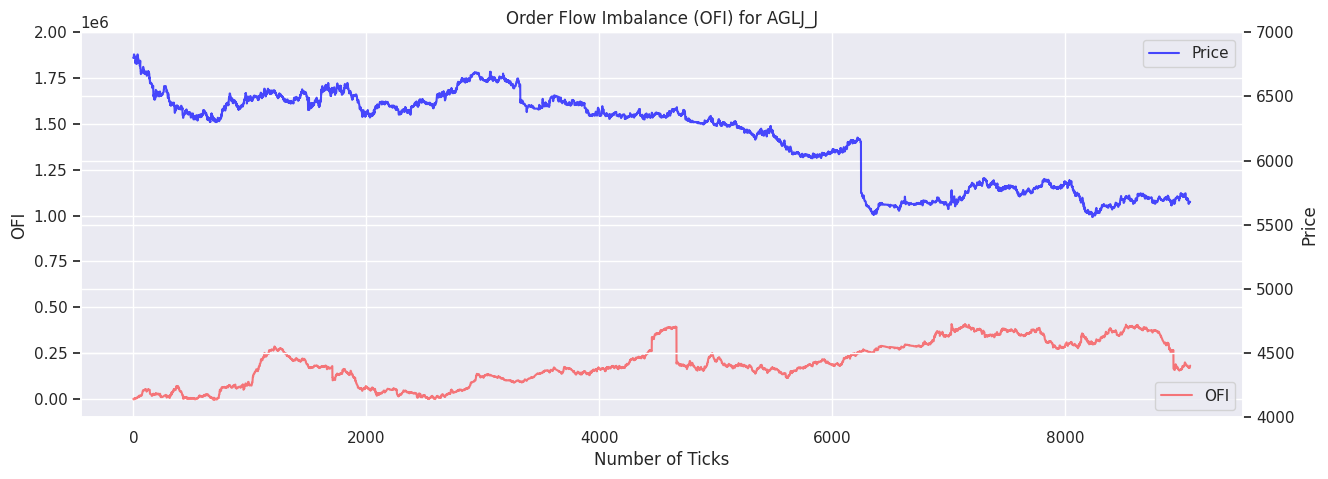
\includegraphics[width=\linewidth,height=0.6\textheight,keepaspectratio]{gfx/m3l3_notes_fig6_order_flow_imbalance.png}
\par\smallskip{\small \textbf{Hình 3.6:} Mất cân bằng dòng lệnh (OFI) lũy kế và giá của AGLJ\_J theo số tick}
\end{figure}

\begin{lstlisting}[escapeinside={(*@}{@*)}]


The Pearson correlation between the price and OFI is:  -0.7586082958132966
\end{lstlisting}

\textbf{Bài tập 5}

Hãy import thư viện \texttt{scipy} và tính tương quan Spearman và Kendall giữa giá và OFI. Bạn thấy gì? Kết quả đó có như bạn kỳ vọng không?

Kết quả trên có phần phản trực giác và rất phổ biến trong thực tế. Nó nhấn mạnh tầm quan trọng của phân tích thực nghiệm với dữ liệu thế giới thực thay vì chỉ dựa vào các kỳ vọng lý thuyết.

Như ta thấy, giá của AGLJ trong năm ngày này có độ dốc đi xuống. Trong một số trường hợp, giá có độ dốc đi lên ngắn hạn, nhưng xu hướng chung là rõ ràng. Với giá như vậy, kỳ vọng của chúng ta (dựa trên lý thuyết và trực giác) sẽ là OFI cũng có độ dốc đi xuống. Nhưng điều này hầu như không xảy ra vì OFI dường như gần như hoàn toàn không nhất quán với giá. Khối lượng mua (theo định nghĩa trong notebook này) đang tăng, nghĩa là có nhiều bên mua (bên nhận lệnh) hơn bên bán, trong khi đồng thời giá lại đang giảm.

Có thể có nhiều lý do cho hiện tượng này, và chúng có thể rất khác nếu dữ liệu được lấy từ một sàn giao dịch khác hoặc cho một khoảng thời gian khác:

\begin{itemize}
  \item Hành vi của nhà tạo lập thị trường/nhà giao dịch: Các nhà tạo lập thị trường hoặc các nhà giao dịch lớn có thể đang cung cấp thanh khoản khi giá giảm, hấp thụ các lệnh bán. Điều này sẽ hiện ra như OFI dương (vì họ đang mua) ngay cả khi giá tiếp tục giảm.
  \item Các giao dịch lớn: Một vài lệnh bán lớn có thể có trọng lượng lớn hơn nhiều lệnh mua nhỏ.
  \item Hiệu ứng vi cấu trúc thị trường: Trong một số cấu trúc thị trường, các lệnh bán lớn có thể kích hoạt một chuỗi các lệnh mua nhỏ hơn khi chúng được khớp, điều này có thể dẫn đến mẫu hình này.
  \item Cân nhắc về khung thời gian: Mối quan hệ giữa OFI và giá có thể khác nhau ở các thang thời gian khác nhau. Những gì ta thấy có thể là một hiệu ứng ngắn hạn có thể đảo chiều trong các giai đoạn dài hơn.
\end{itemize}

\textbf{Bài tập 6}

Chúng ta cố ý đưa ra một định nghĩa cho khối lượng mua và bán: Khối lượng mua/bán là khối lượng của các giao dịch được khởi tạo bởi bên mua/bên bán (với tư cách bên nhận lệnh). Nhưng bây giờ chúng ta phải nghĩ về khối lượng mua và bán từ góc nhìn ý định của nhà giao dịch, tức là khối lượng mua và bán thực sự.

Gợi ý: Nếu một nhà giao dịch muốn mua, họ có thể đặt một lệnh thị trường hoặc một lệnh giới hạn.

Hãy khởi xướng một cuộc thảo luận trên diễn đàn với các ý tưởng của bạn.

\textbf{Bài tập 7}

Chúng ta đã quan sát thấy một kết quả phản trực giác liên quan đến OFI của tập dữ liệu (3): giá giảm trong khi OFI tăng. Bây giờ hãy tính OFI cho tập dữ liệu (2) và vẽ nó cùng với giá trên cùng một đồ thị (hai trục $y$). Bạn thấy gì?

Bây giờ hãy đưa ra các ý tưởng để vẽ giá chào mua và giá chào bán tốt nhất cùng với giá của AGLJ: chúng ta sẽ dùng hàm bậc thang (step) cho các mức báo giá và biểu đồ phân tán (scatter) cho giá.

\begin{lstlisting}[language=Python,escapeinside={(*@}{@*)}]
# (*@Hình@*) 3.7

zoomed_in_quotes_price = aggr_dataset_2.loc['2016-01-04'].iloc[15000:17000, :] # (*@Cắt@*) (*@lát@*) (*@dữ@*) (*@liệu@*)

fig, ax = plt.subplots(figsize=(15, 5))

ax.scatter(x = zoomed_in_quotes_price[(zoomed_in_quotes_price['Type'] == ' Trade') & (zoomed_in_quotes_price['Trade Sign'] == 1)].index, \
              y = zoomed_in_quotes_price[(zoomed_in_quotes_price['Type'] == ' Trade') & (zoomed_in_quotes_price['Trade Sign'] == 1)]['Price'], color='green', \
                label='Buyer initiated Trades', alpha = 0.7, s = 40) # (*@Vẽ@*) (*@các@*) (*@giao@*) (*@dịch@*)
ax.scatter(x = zoomed_in_quotes_price[(zoomed_in_quotes_price['Type'] == ' Trade') & (zoomed_in_quotes_price['Trade Sign'] == -1)].index, \
              y = zoomed_in_quotes_price[(zoomed_in_quotes_price['Type'] == ' Trade') & (zoomed_in_quotes_price['Trade Sign'] == -1)]['Price'], color='red', \
                label='Seller initiated Trades', alpha = 0.7, s = 40) # (*@Vẽ@*) (*@các@*) (*@giao@*) (*@dịch@*)
ax.step(zoomed_in_quotes_price[zoomed_in_quotes_price['Type'] == ' Quote'].index, \
                zoomed_in_quotes_price[zoomed_in_quotes_price['Type'] == ' Quote']['L1 Bid'], color='green', \
                    label='L1 Bid', alpha = 0.8, where = 'post') # (*@Vẽ@*) L1 Bid
ax.step(zoomed_in_quotes_price[zoomed_in_quotes_price['Type'] == ' Quote'].index, \
                zoomed_in_quotes_price[zoomed_in_quotes_price['Type'] == ' Quote']['L1 Ask'], color='red', \
                    label='L1 Ask', alpha = 0.4, where = 'post') # (*@Vẽ@*) L1 Ask

ax.set_title("AGLJ_J trades and L1 Bid/Ask")
ax.set_xlabel("Time")
ax.set_ylabel("Price")
ax.legend()
plt.show()
\end{lstlisting}

% [Nguyên bản không có ảnh kết quả đã lưu cho ô mã Hình 3.7]

\textbf{Bài tập 8}

Trong Hình 3.7, bạn có thể thấy đồ thị các báo giá tốt nhất được vẽ cùng với giá. Hãy làm như sau:
\begin{itemize}
  \item Hãy chắc chắn bạn có thể giải thích đối số \texttt{where = 'post'} bên trong hàm vẽ step.
  \item Bằng cách xem tài liệu của \texttt{matplotlib}, hãy cải tiến đồ thị trên bằng cách điều chỉnh kích thước của marker scatter theo kích thước giao dịch. Cụ thể, nếu giao dịch A lớn hơn giao dịch B thì marker A phải lớn hơn marker B. Bạn có thể chọn một ngày khác và một lát cắt khác của tập dữ liệu. Hãy dán kết quả của bạn lên diễn đàn.
\end{itemize}

\section{Lấy mẫu lại (Resampling)}

Ở mục cuối này, chúng ta sẽ tạo ra các thanh thời gian (time bar) mà ai cũng quen thuộc. Vì lý do này, chúng ta sẽ dùng phương thức \texttt{resample} hoạt động rất tốt với chỉ mục datetime. Chúng ta sẽ tạo các tập dữ liệu cho nhiều khung thời gian và sẽ minh họa cách một số thống kê thay đổi khi khung thời gian lớn dần. Tập dữ liệu chúng ta chọn sẽ là tập dữ liệu (2): rvn\_usdt.

\begin{lstlisting}[language=Python,escapeinside={(*@}{@*)}]
rvn_usdt
\end{lstlisting}

\begin{lstlisting}[language=Python,escapeinside={(*@}{@*)}]
#(*@Tạo@*) (*@hàm@*) (*@resample@*)
def calculate_statistics(df: pd.DataFrame, freq: str) -> dict:
    """
    (*@Tính@*) (*@các@*) (*@thống@*) (*@kê@*) (*@cho@*) (*@một@*) (*@khung@*) (*@thời@*) (*@gian@*) (*@đơn@*) (*@lẻ@*) (*@mà@*) (*@không@*) (*@lưu@*) (*@dữ@*) (*@liệu@*) (*@trung@*) (*@gian@*).
    """
    # (*@Chỉ@*) (*@lấy@*) (*@mẫu@*) (*@lại@*) (*@giá@*) (*@đóng@*) (*@cửa@*) ((*@không@*) (*@phải@*) OHLC)
    resampled_close = df['price'].resample(freq, label='right').last()
    
    # (*@Tính@*) (*@lợi@*) (*@suất@*) (*@log@*)
    log_returns = np.log(resampled_close / resampled_close.shift(1)).dropna()
    
    # (*@Tính@*) (*@và@*) (*@trả@*) (*@về@*) (*@các@*) (*@thống@*) (*@kê@*) (*@ngay@*) (*@lập@*) (*@tức@*)
    stats = {
        'mean': log_returns.mean(),
        'std': log_returns.std(),
        'skewness': log_returns.skew(),
        'kurt': log_returns.kurt()
    }
    
    # (*@Bộ@*) (*@nhớ@*) (*@được@*) (*@giải@*) (*@phóng@*) (*@tự@*) (*@động@*) (*@khi@*) (*@hàm@*) (*@trả@*) (*@về@*)
    return stats

# (*@Xử@*) (*@lý@*) (*@từng@*) (*@khung@*) (*@thời@*) (*@gian@*) (*@một@*)
timeframes = ['1min', '2min', '5min', '10min', '15min', '30min', '1h', '2h', '4h', '8h', '12h', '1D', '2D', '5D']
statistics = {}

for timeframe in timeframes:
    statistics[timeframe] = calculate_statistics(rvn_usdt, timeframe)
\end{lstlisting}

\textbf{Bài tập 9}

Hãy giải thích đối số \texttt{label = right}. Hãy thảo luận các ý tưởng của bạn trên diễn đàn. Ngoài ra, hãy tìm một thư viện phù hợp để vẽ các ``nến'' (candle) cùng với khối lượng.

\begin{lstlisting}[language=Python,escapeinside={(*@}{@*)}]
#(*@Hình@*) 3.8
pd.DataFrame(statistics).T.plot(subplots = True, figsize = (15, 5), layout = (2, 2), title = 'RVN/USDT Price Statistics', alpha = 0.7) # (*@Vẽ@*) (*@các@*) (*@thống@*) (*@kê@*)
plt.show()
\end{lstlisting}

% [Nguyên bản không có ảnh kết quả đã lưu cho ô mã Hình 3.8]

Các kết quả trên phần nào là điều có thể dự đoán và cho ta thấy những tính chất mà ta mất đi hoặc thu được khi tổng hợp dữ liệu tần suất cao.

\begin{itemize}
  \item Lợi suất trung bình gần bằng 0 ở các khung thời gian nhỏ. Vì mỗi giao dịch tương ứng với các bước giá nhỏ, nên tự nhiên là các thay đổi giá ở khung thời gian nhỏ không thể tích lũy để cho thấy một giá trị trung bình khác không.
  \begin{enumerate}
    \item Nhiễu vi cấu trúc thị trường (Microstructure Noise): Ở tần suất rất cao, lợi suất chịu ảnh hưởng nặng nề của các hiệu ứng vi cấu trúc thị trường như hiện tượng nảy giá chào mua-chào bán (bid-ask bounce), có thể che lấp bất kỳ xu hướng giá thực sự nào trong các khoảng ngắn.
    \item Tính chất martingale (Martingale Property): Trong một thị trường công bằng, các quá trình giá thường được mô hình hóa như martingale, trong đó giá kỳ vọng trong tương lai, cho trước mọi thông tin quá khứ, chính là giá hiện tại. Điều này hàm ý rằng lợi suất kỳ vọng ngắn hạn phải bằng không.
  \end{enumerate}
  \item Độ lệch chuẩn (Standard Deviation): Việc độ lệch chuẩn tăng theo khung thời gian lớn hơn phù hợp với các tính chất của chuyển động Brown (Brownian motion) (xem thêm trong môn Định giá Phái sinh), vốn được dùng để mô hình hóa các quá trình giá. Theo các giả định của chuyển động Brown, phương sai tăng tuyến tính theo thời gian, do đó độ lệch chuẩn tăng theo căn bậc hai của thời gian.
  \item Độ dốc đi lên nhẹ của độ lệch (skewness) khi khung thời gian lớn dần có thể cho thấy rằng các biến động giá dương có xu hướng lớn hơn các biến động giá âm trong các giai đoạn dài hơn.
  \item Quan trọng hơn, độ nhọn (kurtosis) cao ở các khung thời gian nhỏ phản ánh bản chất nhọn (leptokurtic) của lợi suất tần suất cao. Cụ thể hơn:
  \begin{enumerate}
    \item Đuôi béo (Fat Tails): Các sự kiện cực đoan xảy ra phổ biến trong phân phối nhọn, phổ biến hơn so với phân phối chuẩn.
    \item Khi ta tổng hợp lên các khung thời gian lớn hơn, định lý giới hạn trung tâm phát huy tác dụng và phân phối lợi suất tiến gần đến phân phối chuẩn. Tuy nhiên, ở các khung thời gian lớn hơn, lợi suất vẫn chưa đạt tới phân phối chuẩn.
  \end{enumerate}
\end{itemize}

\textbf{Bài tập 10}

Hãy tạo các thanh thời gian cho cặp rvn\_usdt như ở trên nhưng bây giờ thêm hai cột nữa:
\begin{itemize}
  \item Một cột tên \texttt{buying\_volume} gồm khối lượng tổng hợp của các giao dịch thuộc \texttt{is\_buyer\_maker = False}
  \item Một cột tên \texttt{selling\_volume} gồm khối lượng tổng hợp của các giao dịch thuộc \texttt{is\_buyer\_maker = True}
\end{itemize}

\textbf{Bài tập 11}

Khi giải thích các thống kê của Hình 3.8, chúng ta đã dùng định lý giới hạn trung tâm để lập luận cho sự hội tụ của phân phối lợi suất về phân phối chuẩn. Nhưng thực ra chúng ta không hề tổng hợp các lợi suất. Thay vào đó, chúng ta dùng cột \texttt{close} của mỗi khung thời gian để tính độ nhọn. Lập luận đó có được dùng đúng hay không? Vì sao? Hãy làm như trên nhưng thay vì giá \texttt{close} của mỗi khung thời gian, hãy tính \texttt{sum()} của các lợi suất log. Điều này có thay đổi gì không?

\section{Kết luận}

Bài học này đã cung cấp phần giới thiệu về dữ liệu tick, các đặc điểm của nó và tầm quan trọng của nó trong các thị trường tài chính. Chúng ta đã khám phá cấu trúc của dữ liệu giao dịch từng tick và dữ liệu Level 1, minh họa cách xử lý, làm sạch và vẽ các tập dữ liệu tần suất cao này.

Những điểm chính cần ghi nhớ gồm:

\begin{enumerate}
  \item Độ chi tiết của dữ liệu tick mang lại những hiểu biết về vi cấu trúc thị trường mà không thể thấy được trong dữ liệu tần suất thấp hơn.
  \item Làm sạch là một bước tiền xử lý thiết yếu, cần bao gồm việc xử lý các giao dịch bị chia nhỏ và các báo giá trong cùng một giây (cùng nhiều vấn đề khác).
  \item Mất cân bằng dòng lệnh (OFI) có thể cung cấp những hiểu biết có giá trị về động lực thị trường ngắn hạn, nhưng việc diễn giải nó đòi hỏi cân nhắc cẩn thận bối cảnh thị trường và có thể gây hiểu lầm.
  \item Lấy mẫu lại dữ liệu tick sang nhiều khung thời gian cho thấy các tính chất thống kê của lợi suất thay đổi ra sao theo sự tổng hợp thời gian, làm nổi bật sự đánh đổi giữa độ chi tiết và nhiễu.
  \item Làm việc với dữ liệu tick đặt ra những thách thức riêng, bao gồm khối lượng dữ liệu, các yêu cầu làm sạch, và nhu cầu về các kỹ thuật phân tích chuyên biệt.
\end{enumerate}

\textbf{Tài liệu tham khảo}

\begin{itemize}
  \item Gebbie, Tim, and Edward Nonyane. ``TRTH JSE AGLJ.J Intraday Transaction Test Data.'' Mendeley Data, V2, 2019.
  \item Harris, Larry. \emph{Trading and Exchanges: Market Microstructure for Practitioners}. Oxford University Press, 2003.
  \item Hautsch, Nikolaus. \emph{Econometrics of Financial High-Frequency Data}. Springer Science \& Business Media, 2011.
\end{itemize}

\chapter{Đọc thêm 1: Quy trình Làm sạch Dữ liệu Tần suất Cao (Barndorff-Nielsen et al.)}
\label{ch:M3L3DT1}

% Nguồn: Barndorff-Nielsen, O. E., Hansen, P. R., Lunde, A., & Shephard, N. ``Realized Kernels in Practice: Trades and Quotes.'' Econometrics Journal, vol. 12, 2009, pp. C1-C32.
% Phần cần đọc: Trang C7-C8
% Nội dung bắt buộc đọc: được kiểm tra trong mọi bài đánh giá (kể cả Quiz).

\section{Thông tin nguồn}

\begin{itemize}
  \item \textbf{Nguồn:} Barndorff-Nielsen, O. E., et al. \emph{Realized Kernels in Practice: Trades and Quotes}. Econometrics Journal, vol. 12, 2009. \url{https://onlinelibrary.wiley.com/doi/epdf/10.1111/j.1368-423X.2008.00275.x}
  \item \textbf{Phần cần đọc:} Trang C7-C8
\end{itemize}

\section{3. Quy trình làm sạch dữ liệu tần suất cao}

Làm sạch dữ liệu cẩn thận là một trong những khía cạnh quan trọng nhất khi ước lượng biến động từ dữ liệu tần suất cao. Làm sạch dữ liệu tần suất cao đã nhận được sự chú ý đặc biệt, chẳng hạn trong Dacorogna et al. (2001, chương 4), Falkenberry (2001), Hansen và Lunde (2006), và Brownlees và Gallo (2006). Cụ thể, Hansen và Lunde (2006) cho thấy việc loại bỏ một số lượng lớn quan sát trên thực tế có thể cải thiện các ước lượng biến động. Kết quả này thoạt nhìn có vẻ phản trực giác, nhưng lý do khá đơn giản. Một ước lượng sử dụng tối ưu toàn bộ dữ liệu thường sẽ đặt trọng số cao cho dữ liệu chính xác và ít bị ảnh hưởng bởi các quan sát kém chính xác nhất. Ước lượng bình phương tối thiểu tổng quát (generalized least-squares, GLS) trong mô hình hồi quy cổ điển là một phép tương tự tốt cho điều này. Mặt khác, độ chính xác của ước lượng bình phương tối thiểu thông thường có thể xấu đi khi các quan sát tương đối nhiễu được đưa vào ước lượng. Vì vậy, việc đưa vào các quan sát chất lượng kém có thể gây hại nhiều hơn là có lợi cho ước lượng bình phương tối thiểu thông thường, và đây chính là phép so sánh phù hợp với tình huống hiện tại. Realized kernel và các ước lượng liên quan ``đối xử với tất cả các quan sát như nhau'', và một vài giá trị ngoại lai cũng có thể ảnh hưởng nghiêm trọng đến các ước lượng này.

\subsection*{3.1. Quy trình làm sạch từng bước}

Trong phân tích thực nghiệm của chúng tôi, chúng tôi sử dụng dữ liệu giao dịch và báo giá từ cơ sở dữ liệu Trade and Quote (TAQ) của NYSE, với mục tiêu ước lượng biến phân toàn phương (quadratic variation) cho khoảng thời gian từ 9:30 sáng đến 4 giờ chiều. Việc làm sạch dữ liệu tần suất cao TAQ được thực hiện theo các bước sau. Các quy tắc P1 đến P3 được áp dụng cho cả dữ liệu giao dịch lẫn dữ liệu báo giá, các quy tắc T1 đến T4 chỉ áp dụng cho dữ liệu giao dịch, còn các quy tắc Q1 đến Q4 chỉ áp dụng cho dữ liệu báo giá.

\subsubsection*{Tất cả dữ liệu}

\begin{itemize}
  \item[\textbf{P1.}] Xóa các mục có dấu thời gian nằm ngoài khung 9:30 sáng đến 4 giờ chiều, tức giờ mở cửa của sàn giao dịch.
  \item[\textbf{P2.}] Xóa các mục có giá chào mua (bid), giá chào bán (ask) hoặc giá giao dịch bằng 0.
  \item[\textbf{P3.}] Chỉ giữ lại các mục có nguồn gốc từ một sàn giao dịch duy nhất (NYSE, trong ứng dụng của chúng tôi). Xóa các mục còn lại.
\end{itemize}

\subsubsection*{Chỉ dữ liệu báo giá}

\begin{itemize}
  \item[\textbf{Q1.}] Khi nhiều báo giá có cùng dấu thời gian, chúng tôi thay thế tất cả các báo giá đó bằng một mục duy nhất, sử dụng giá chào mua trung vị và giá chào bán trung vị.
  \item[\textbf{Q2.}] Xóa các mục có mức chênh lệch giá (spread) âm.
  \item[\textbf{Q3.}] Xóa các mục có mức chênh lệch giá lớn hơn 50 lần mức chênh lệch giá trung vị của ngày hôm đó.
  \item[\textbf{Q4.}] Xóa các mục có giá giữa (mid-quote) lệch nhiều hơn 10 lần độ lệch tuyệt đối trung bình so với trung vị cuộn có tâm (rolling centred median, không tính quan sát đang xét) của 50 quan sát (25 quan sát trước và 25 quan sát sau).
\end{itemize}

\subsubsection*{Chỉ dữ liệu giao dịch}

\begin{itemize}
  \item[\textbf{T1.}] Xóa các mục có giao dịch đã được đính chính. (Các giao dịch có \emph{Chỉ báo Đính chính} (Correction Indicator), CORR $\neq$ 0).
  \item[\textbf{T2.}] Xóa các mục có \emph{Điều kiện Bán} (Sale Condition) bất thường. (Các giao dịch mà COND mang mã chữ cái, ngoại trừ 'E' và 'F'). Xem TAQ 3 User's Guide để biết thêm chi tiết về các điều kiện bán.
  \item[\textbf{T3.}] Nếu nhiều giao dịch có cùng dấu thời gian, sử dụng giá trung vị.
  \item[\textbf{T4.}] Xóa các mục có giá cao hơn giá ``ask'' cộng với mức chênh lệch giá chào mua chào bán (bid-ask spread). Tương tự đối với các mục có giá thấp hơn giá ``bid'' trừ đi mức chênh lệch giá chào mua chào bán.
\end{itemize}

\subsection*{3.2. Thảo luận về các quy tắc lọc}

Bước đầu tiên, P1, xác định các mục liên quan đến phân tích của chúng tôi, vốn tập trung vào biến động trong khoảng 9:30 sáng đến 4 giờ chiều.

Các bước P2 và T1 loại bỏ những lỗi rất nghiêm trọng trong cơ sở dữ liệu, chẳng hạn như ghi sai giá (ví dụ giá bằng 0 hoặc đặt sai vị trí dấu thập phân), và các dấu thời gian có thể sai lệch đáng kể. T2 loại bỏ các điểm dữ liệu mà cơ sở dữ liệu TAQ đang gắn cờ là có vấn đề. Bảng 1 tóm tắt số lượng dữ liệu bị xóa hoặc được tổng hợp bằng các quy tắc lọc này đối với cơ sở dữ liệu được sử dụng trong Mục 4, phân tích cổ phiếu Alcoa.

Quan trọng hơn cả ở đây là các quy tắc P3, T3 và Q1. Trong công trình thực nghiệm của chúng tôi, chúng tôi sẽ xem xét tác động của việc tạm ngưng áp dụng P3. Quy tắc này được dùng để giảm tác động của độ trễ thời gian trong việc báo cáo giao dịch và cập nhật báo giá. Một dạng nào đó của quy tắc T3 và Q1 dường như là không thể tránh khỏi ở đây, và chính các quy tắc này dẫn đến lượng dữ liệu bị xóa lớn nhất.

Chúng tôi sử dụng Q4 để bắt các giá trị ngoại lai mà Q3 bỏ sót. Bằng cách xây dựng cửa sổ dựa trên số lượng quan sát, chúng tôi để cửa sổ đó giãn ra và co lại theo thời gian đồng hồ (clock time) tùy cường độ giao dịch. Việc lựa chọn 50 quan sát cho cửa sổ là \emph{tùy ý theo kinh nghiệm} (\emph{ad hoc}), nhưng đã được kiểm chứng qua thực nghiệm mở rộng.

T4 là một quy tắc hấp dẫn, vì nó kiểm soát chặt dữ liệu giao dịch bằng dữ liệu báo giá. Tuy nhiên, nó có nhược điểm là không thể áp dụng được khi không có sẵn dữ liệu báo giá.\footnote{Khi không có sẵn dữ liệu báo giá, Q4 có thể được áp dụng thay cho T4, bằng cách thay mid-quote (giá giữa) bằng price (giá).} Bảng 1 cho thấy quy tắc này hiếm khi được kích hoạt trong thực tế, trong khi các kết quả sau này mà chúng tôi sẽ thảo luận ở Bảng 2 về realized kernel cho thấy ước lượng RK (khác với thống kê RV) không nhạy cảm lắm với việc sử dụng T4.

Việc so sánh một số quy tắc lọc của chúng tôi với các quy tắc được Falkenberry (2001) và Brownlees và Gallo (2006) đề xuất là điều thú vị. Trong sự so sánh như vậy, các quy tắc được thiết kế để loại bỏ giá trị ngoại lai hoặc dữ liệu ghi sai là những quy tắc có thể gây tranh cãi.

Trong số các quy tắc của chúng tôi, Q4 và T4 là những quy tắc liên quan. Q4 có liên hệ rất chặt chẽ với quy trình mà Brownlees và Gallo (2006, tr. 2237) đề xuất để loại bỏ giá trị ngoại lai. Họ loại bỏ quan sát $i$ nếu điều kiện $|p_i - \bar{p}_i(k)| > 3 s_i(k) + \gamma$ được thỏa mãn. Ở đây, $\bar{p}_i(k)$ và $s_i(k)$ lần lượt biểu thị trung bình mẫu $\delta$-cắt ($\delta$-trimmed sample mean) và độ lệch chuẩn mẫu của một lân cận gồm $k$ quan sát xung quanh $i$, còn $\gamma$ là một tham số hạt (granularity parameter). Chúng tôi sử dụng trung vị thay cho trung bình mẫu đã cắt $\bar{p}_i(k)$, và độ lệch tuyệt đối trung bình so với trung vị thay cho $s_i(k)$. Bằng cách không sử dụng độ lệch chuẩn mẫu, phương pháp của chúng tôi ít nhạy cảm hơn với các chuỗi giá trị ngoại lai liên tiếp (runs of outliers).

Falkenberry (2001) cũng sử dụng một cách tiếp cận ngưỡng để xác định liệu một quan sát nhất định có phải là giá trị ngoại lai hay không. Nhưng thay vì sử dụng phương pháp ``Tìm kiếm và Loại bỏ'' (Search and Purge), ông áp dụng phương pháp luận ``Tìm kiếm và Chỉnh sửa'' (Search and Modify). Các mức giá lệch một lượng nhất định so với bộ lọc trượt (moving filter) của tất cả các mức giá sẽ được chỉnh sửa lại thành giá trị của bộ lọc. Đối với các giao dịch, cách này có ưu điểm là duy trì được khối lượng của một giao dịch ngay cả khi mức giá liên quan là sai.

Cuối cùng, chúng tôi lưu ý rằng cách tiếp cận của chúng tôi trong việc kiểm soát chặt chẽ dữ liệu giao dịch bằng dữ liệu báo giá, tức quy tắc T4, trước đây mới chỉ được áp dụng trong Hansen và Lunde (2006), Barndorff-Nielsen et al. (2006), và Barndorff-Nielsen et al. (2008a).
</content>

\chapter{Đọc thêm 2: Xử lý Dữ liệu Tần suất Siêu cao (Brownlees \& Gallo)}
\label{ch:M3L3DT2}

% Nguồn: Brownlees, C. T., & Gallo, G. M. ``Financial Econometric Analysis at Ultra-High Frequency: Data Handling Concerns.'' Computational Statistics & Data Analysis, 51(4), 2006, pp. 2232-2245.
% Phần cần đọc: Sections 3.1-3.2
% Nội dung bắt buộc đọc: được kiểm tra trong mọi bài đánh giá (kể cả Quiz).

\section{Thông tin nguồn}

\begin{itemize}
  \item \textbf{Nguồn:} Brownlees, Christian T., and Giampiero M. Gallo. \emph{Financial Econometric Analysis at Ultra-High Frequency: Data Handling Concerns}. Computational Statistics \& Data Analysis, vol. 51, no. 4, 2006, pp. 2232-2245. \url{https://papers.ssrn.com/sol3/papers.cfm?abstract_id=886204}
  \item \textbf{Phần cần đọc:} Sections 3.1-3.2
\end{itemize}

\section{3.1 Làm sạch Dữ liệu}

\begin{figure}[H]
\centering
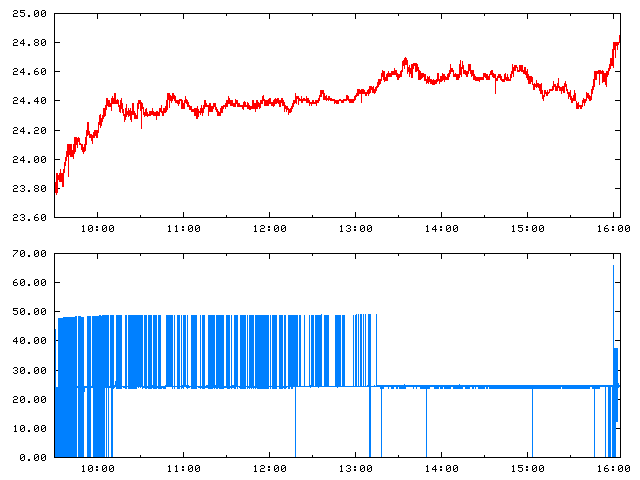
\includegraphics[width=0.7\linewidth]{gfx/m3l3_brownlees_fig1_trade_quote_oneday.png}
\par\smallskip{\small \textbf{Hình 1:} Dữ liệu giao dịch và báo giá của cổ phiếu General Electric vào ngày 11 tháng 11 năm 2002, từ 9:30:00 sáng đến 4:05:00 chiều. Chuỗi giá giao dịch theo từng tick (trên); chuỗi giá chào mua và chào bán theo từng tick (dưới).}
\end{figure}

Dữ liệu tần suất siêu cao (UHFD) thô vốn nổi tiếng là dễ chứa sai số, do đó cần áp dụng một phương pháp phát hiện và loại bỏ các giá trị sai số này trước khi tiến hành phân tích chuỗi thời gian. Thao tác xử lý dữ liệu sơ bộ này thường được gọi là lọc dữ liệu (filtering) hoặc làm sạch dữ liệu (data cleaning). Mục tiêu của nó là loại bỏ khỏi chuỗi thời gian tần suất siêu cao mọi quan sát không phản ánh đúng hoạt động thị trường thực tế; tuy nhiên trên thực tế, các phương pháp này dường như chỉ dừng ở mức phát hiện giá trị ngoại lai (outlier).

\begin{figure}[H]
\centering
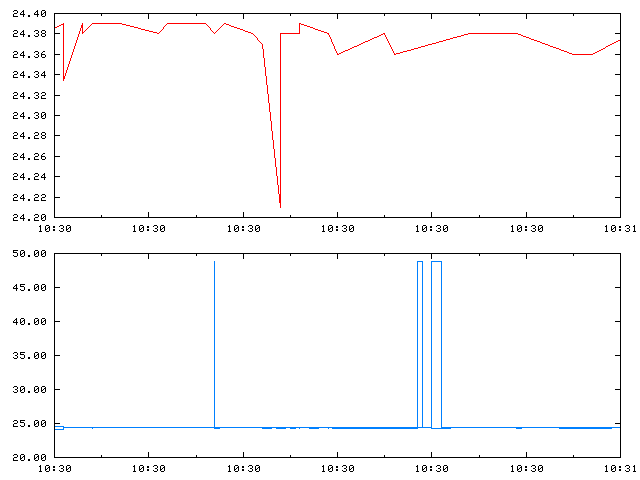
\includegraphics[width=0.7\linewidth]{gfx/m3l3_brownlees_fig2_trade_quote_oneminute.png}
\par\smallskip{\small \textbf{Hình 2:} Dữ liệu giao dịch và báo giá của cổ phiếu General Electric vào ngày 11 tháng 11 năm 2002, từ 10:30:00 sáng đến 10:31:00 sáng. Chuỗi giá giao dịch theo từng tick (trên); chuỗi giá chào mua và chào bán theo từng tick (dưới).}
\end{figure}

Nguồn gốc của các sai số này không thực sự rõ ràng. Falkenberry (2002) cho biết sai số xuất hiện cả trong các hệ thống giao dịch tự động hoàn toàn lẫn tự động một phần, chẳng hạn như Sàn Giao dịch Chứng khoán New York (NYSE). Theo tác giả này, cường độ giao dịch là yếu tố quyết định chính gây ra sai số: tốc độ giao dịch càng cao thì xác suất xảy ra sai sót khi báo cáo thông tin giao dịch càng lớn.

Phần lớn các quy trình làm sạch dữ liệu chỉ xử lý chuỗi giá theo từng giao dịch (tick-by-tick). Điều này có lẽ xuất phát từ việc tuy ``dễ dàng'' đánh giá một mức giá có phù hợp với điều kiện thị trường hiện tại hay không, nhưng lại khó hơn nhiều để đánh giá tính hợp lý của một khối lượng giao dịch nhất định. Do đó, đối với dữ liệu khối lượng, không có công thức làm sạch dữ liệu đặc thù nào ngoài việc đánh giá tính hợp lý của khối lượng dựa trên tính hợp lý của mức giá tương ứng, kết hợp với các phương pháp phát hiện giá trị ngoại lai thống kê cổ điển.

Hình 1 và Hình 2 lần lượt thể hiện dữ liệu giá giao dịch và báo giá của cổ phiếu General Electric trong một ngày và trong một phút. Có thể thấy dữ liệu giao dịch (trade) chính xác hơn nhiều so với dữ liệu báo giá (quote). Phù hợp với nhận định của Falkenberry (2002), một cách giải thích khả dĩ cho hiện tượng này là trong một ngày giao dịch, số lượng báo giá lớn hơn nhiều so với số lượng giao dịch thực hiện. Một cách giải thích khác là dữ liệu giao dịch ghi nhận các hợp đồng đã thực sự được khớp lệnh, chứ không chỉ là các đề nghị trao đổi đơn thuần, do đó các chủ thể thị trường thận trọng hơn nhiều khi báo cáo loại thông tin này so với báo giá. Một điểm đáng chú ý ở hai hình trên là chúng dường như cho thấy ít nhất một số sai số trong chuỗi dữ liệu là rất rõ ràng, dễ nhận thấy.

Trong các tài liệu đã có, một số thuật toán được đề xuất để loại bỏ các quan sát sai (xem Dacorogna et al. (2001) về thuật toán được Olsen \& Associates sử dụng để thực hiện công việc này trên dữ liệu tỷ giá hối đoái, vốn có vẻ phức tạp hơn nhiều so với mức cần thiết cho dữ liệu NYSE). Zhou (1996) đề cập một phương pháp đơn giản để kiểm định dữ liệu báo giá ngoại hối bằng cách so sánh mỗi báo giá với trung vị của ba quan sát liền trước và ba quan sát liền sau, rồi loại bỏ báo giá đó nếu nó nằm ngoài một khoảng cách cố định so với các trung vị này.

Thay vào đó, chúng tôi đề xuất một quy trình đã cho kết quả khả quan, như sẽ trình bày dưới đây. Gọi $\{p_i\}_{i=1}^{N}$ là một chuỗi giá theo từng giao dịch (tick-by-tick) đã được sắp xếp theo thứ tự. Quy trình mà chúng tôi đề xuất để loại bỏ giá trị ngoại lai là

\[
\big(\,|p_i - \bar{p}_i(k)| < 3\,s_i(k) + \gamma\,\big) =
\begin{cases}
\text{true} & \text{quan sát } i \text{ được giữ lại} \\
\text{false} & \text{quan sát } i \text{ bị loại bỏ}
\end{cases}
\]

trong đó $\bar p_i(k)$ và $s_i(k)$ lần lượt ký hiệu trung bình mẫu đã cắt tỉa 10\% (10\% trimmed mean) và độ lệch chuẩn mẫu của một vùng lân cận gồm $k$ quan sát xung quanh $i$, còn $\gamma$ là một \textit{tham số độ chi tiết} (granularity). Vùng lân cận các quan sát luôn được chọn sao cho một quan sát nhất định chỉ được so sánh với các quan sát thuộc cùng ngày giao dịch. Cụ thể, vùng lân cận của quan sát đầu tiên trong ngày là $k$ tick đầu tiên của ngày, vùng lân cận của quan sát cuối cùng trong ngày là $k$ tick cuối cùng của ngày, còn vùng lân cận của một giao dịch bất kỳ ở giữa ngày được tạo thành xấp xỉ bởi $k/2$ tick liền trước và $k/2$ tick liền sau, và tương tự như vậy cho các trường hợp khác. Ý tưởng đằng sau thuật toán này là đánh giá tính hợp lệ của một quan sát dựa trên khoảng cách tương đối của nó so với một vùng lân cận gồm các quan sát hợp lệ gần nhất. Vai trò của tham số $\gamma$ đặc biệt quan trọng. Các chuỗi dữ liệu tần suất siêu cao thường chứa các dãy giá bằng nhau liên tiếp, điều này khiến phương sai bằng 0; do đó, nên đưa vào một cận dưới dương cho các biến động giá luôn được xem là hợp lệ.

Cần lưu ý một số điểm quan trọng về việc lựa chọn các tham số của thuật toán, đó là $k$ và $\gamma$. Tham số $k$ nên được chọn dựa trên mức độ sôi động của giao dịch. Nếu giao dịch không quá sôi động, $k$ nên được chọn ``tương đối nhỏ'' để cửa sổ quan sát không chứa những mức giá quá xa nhau về thời gian. Ngược lại, nếu giao dịch rất sôi động, $k$ nên được chọn ``tương đối lớn'' để cửa sổ quan sát chứa đủ số lượng quan sát nhằm ước lượng chính xác các đặc điểm cục bộ của giá. Việc lựa chọn $\gamma$ nên là một bội số của mức biến động giá tối thiểu được phép đối với cổ phiếu cụ thể đang xét.

Quy trình này chắc chắn mang tính kinh nghiệm (heuristic), nhưng có ưu điểm là đơn giản và hiệu quả: chúng tôi sẽ cho thấy mức độ nhạy của một ví dụ minh họa trước cách chọn các tham số nói trên.

\section{3.2 Quản lý Dữ liệu}

Ngay cả khi UHFD đã được ``làm sạch'', việc xây dựng chuỗi thời gian phù hợp cho mục đích phân tích vẫn có thể khá phức tạp, bởi vì

\begin{itemize}
  \item dữ liệu có cấu trúc phức tạp, và
  \item không phải lúc nào cũng có một cách duy nhất và tối ưu để tổng hợp thông tin.
\end{itemize}

Trong các đoạn tiếp theo, chúng tôi sẽ trình bày một số đặc điểm riêng biệt xuất hiện trong dữ liệu cùng các phương pháp được đề xuất để xử lý chúng.

\noindent\textbf{Quan sát đồng thời.} Hình 3 trình bày 1 phút dữ liệu tần suất siêu cao gồm giá giao dịch, log-khối lượng giao dịch và hai chuỗi giá chào mua, giá chào bán. Lưu ý rằng mỗi dấu cộng trên đường giá giao dịch đánh dấu một giao dịch. Có thể thấy rằng có nhiều giao dịch được báo cáo tại cùng một thời điểm nhưng được khớp ở các mức giá khác nhau. Nhiều mức giá đồng thời khác nhau cũng xuất hiện trong dữ liệu báo giá.

\begin{figure}[H]
\centering
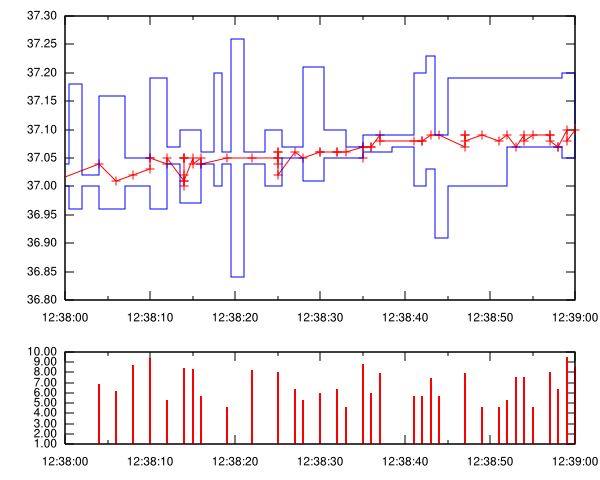
\includegraphics[width=0.7\linewidth]{gfx/m3l3_brownlees_fig3_trading_activity_minute.png}
\par\smallskip{\small \textbf{Hình 3:} Một phút hoạt động giao dịch của cổ phiếu General Electric vào ngày 21 tháng 3 năm 2002, từ 12:38 đến 12:39 chiều. Giá giao dịch nằm trong khoảng giá chào mua-chào bán (bảng trên). Mỗi dấu cộng trên đường giá giao dịch đánh dấu một giao dịch khác nhau. Log-khối lượng gắn với từng giao dịch (bảng dưới).}
\end{figure}

Có nhiều cách giải thích khác nhau cho hiện tượng này. Trước hết, cần lưu ý rằng các chứng khoán niêm yết trên NYSE cũng có thể được giao dịch trên các sàn khác, do đó việc có giao dịch và báo giá đồng thời ở các mức giá khác nhau là điều bình thường. Một cách giải thích khác cho hiện tượng này đối với dữ liệu giao dịch là việc khớp lệnh thị trường trên một sàn giao dịch đôi khi tạo ra nhiều hơn một báo cáo giao dịch. Cách giải thích thứ ba, cũng là cuối cùng, là ngay cả những giao dịch/báo giá không thực sự đồng thời cũng có thể bị ghi nhận là đồng thời do các sai số xấp xỉ khi báo cáo. Do đó, trên thực tế, rất thường gặp trường hợp có nhiều hơn một giao dịch và báo giá được báo cáo tại cùng một mốc thời gian.

Vì các mô hình tần suất siêu cao dùng để mô hình hóa dữ liệu tick-by-tick thường chỉ cần một quan sát cho mỗi mốc thời gian, nên cần thực hiện một hình thức tổng hợp (aggregation) nào đó. Đối với chuỗi giá tick-by-tick, thứ tự của các quan sát đồng thời được báo cáo dường như không mang nhiều ý nghĩa đặc biệt. Lấy giá trung vị có thể là một giải pháp hợp lý, xét đến bản chất rời rạc của dữ liệu tick-by-tick. Nếu sau đó còn tổng hợp thêm xuống các tần suất thấp hơn, việc chọn phương pháp tổng hợp càng ít quan trọng vì chênh lệch giữa các mức giá là không đáng kể, và các phương pháp đơn giản hơn như lấy giá cuối cùng hoặc giá đầu tiên của dãy quan sát cũng không nên gây ra vấn đề nào. Đối với khối lượng giao dịch hoặc số lượng giao dịch theo tick-by-tick, cách tổng hợp tự nhiên là thay thế các quan sát đồng thời bằng tổng khối lượng đồng thời và số lượng giao dịch đồng thời.

\noindent\textbf{Dữ liệu cách quãng không đều.} Đặc điểm nổi bật nhất của dữ liệu trình bày trong Hình 3 là các chuỗi thời gian được vẽ không đều đặn (irregular), nghĩa là khoảng thời gian phân cách hai quan sát liên tiếp là ngẫu nhiên. Thay vì làm việc trực tiếp với các quan sát tần suất siêu cao có khoảng cách thời gian không đều cho nhiều loại nghiên cứu khác nhau, người ta có thể muốn phân tích một chuỗi thời gian rời rạc với các khoảng thời gian cách đều nhau.

Gọi $\{(t_i,y_i)\}_{i=1}^{N}$ là một chuỗi thời gian không đều, trong đó $t_i$ và $y_i$ lần lượt biểu thị thời điểm và giá trị của quan sát thứ $i$, và gọi $\{(t_j^{*},y_j^{*})\}_{j=1}^{N^{*}}$ là chuỗi thời gian tần suất thấp hơn mà ta muốn xây dựng. Khi đó, vấn đề đặt ra là dùng một hàm tổng hợp phù hợp, tận dụng thông tin tần suất cao để thu được chuỗi quan sát $\{y_j^{*}\}_{j=1}^{N^{*}}$ của chuỗi đều. Vì ta đang tổng hợp thông tin tần suất cao xuống tần suất thấp hơn, dùng các hàm tổng hợp có dạng như sau có vẻ hợp lý:

\[
y_j^{*} = f\big(\{(t_i,y_i) \mid t_i \in (t_{j-1}^{*}, t_j^{*}]\}\big)
\]

điều này về cơ bản hàm ý rằng giá trị quan sát tổng hợp $y_j^{*}$ được xây dựng dựa trên toàn bộ thông tin sẵn có kể từ quan sát trước đó tại $t_{j-1}^{*}$ cho đến $t_j^{*}$.\footnote{Lưu ý rằng $f$ cũng có thể được định nghĩa thay thế như một hàm của $\{(t_i,y_i) \mid t_i \in [t_j^{*}, t_{j+1}^{*}), i=1,...,N\}$. Đây chỉ là vấn đề quy ước ký hiệu.}

Một số phương pháp đơn giản nhưng hữu ích, phù hợp với cách tiếp cận này, là:

\textbf{First:} $y_j^{*} = x_f$ trong đó $t_f = \min\{t_i \mid t_i \in (t_{j-1}^{*}, t_j^{*}]\}$

\textbf{Minimum:} $y_j^{*} = \min\{y_i \mid t_i \in (t_{j-1}^{*}, t_j^{*}]\}$

\textbf{Maximum:} $y_j^{*} = \max\{y_i \mid t_i \in (t_{j-1}^{*}, t_j^{*}]\}$

\textbf{Last:} $y_j^{*} = x_l$ trong đó $t_l = \max\{t_i \mid t_i \in (t_{j-1}^{*}, t_j^{*}]\}$

\textbf{Sum:} $y_j^{*} = \sum_{t_i \in (t_{j-1}^{*}, t_j^{*}]} y_i$

\textbf{Count:} $y_j^{*} = \#\{(y_i,t_i) \mid t_i \in (t_{j-1}^{*}, t_j^{*}]\}$

Trong bốn phương pháp đầu tiên, nếu tập $\{t_i \mid t_i \in [t_j^{*}, t_{j+1}^{*})\}$ rỗng thì quan sát thứ $j$ sẽ được coi là bị thiếu (missing). Các phương pháp ``First'', ``Minimum'', ``Maximum'' và ``Last'' có thể hữu ích khi xử lý chuỗi giá. Phương pháp ``Sum'' phù hợp để tổng hợp khối lượng, còn ``Count'' có thể được dùng để xác định số lượng giao dịch và báo giá.

Riêng đối với việc xây dựng chuỗi giá đều, Dacorogna et al. (2001) đề xuất một số phương pháp dựa trên việc nội suy tại $t_j^{*}$ từ quan sát liền trước và liền sau trong chuỗi:

\textbf{Previous Point Interpolation:} $y_j^{*} = y_p$ trong đó $t_p = \max\{t_i \mid t_i < t_j^{*}\}$

\textbf{Next Point Interpolation:} $y_j^{*} = y_n$ trong đó $t_n = \min\{t_i \mid t_i > t_j^{*}\}$

\textbf{Linear Point Interpolation:} $y_j^{*} = y_p + \dfrac{t_j^{*} - t_p}{t_n - t_p}(y_n - y_p)$

Tuy nhiên, vấn đề của các phương pháp này là chúng có thể dùng thông tin không thực sự có sẵn tại thời điểm $t_j^{*}$. Đối với các cổ phiếu thanh khoản cao, việc lựa chọn sơ đồ nội suy dường như không quá quan trọng vì vùng lân cận của $t^{*}$ sẽ chứa rất nhiều quan sát dày đặc, và các sơ đồ nội suy khác nhau sẽ cho kết quả xấp xỉ giống với phương pháp ``Last''. Ngược lại, kết quả có thể rất khác nhau đối với các cổ phiếu ít được giao dịch. Với các cổ phiếu này, chúng tôi cho rằng các sơ đồ nội suy không hoàn toàn thỏa đáng. Giả sử ta đang xây dựng một chuỗi giá tần suất cao có khoảng cách đều, chẳng hạn 5 phút. Điều thường xảy ra đối với các cổ phiếu ít được giao dịch và trong thời gian tạm ngừng giao dịch (halt) là sẽ có một số khoảng, chẳng hạn $(t_{j-1}^{*}, t_j^{*}]$, không chứa bất kỳ quan sát nào; do đó, trong trường hợp nội suy theo điểm liền trước, mức giá nội suy tại $t_j^{*}$ có thể thực chất là một mức giá thuộc về một thời điểm trước đó khá xa, chẳng hạn $(t_{j-k-1}^{*}, t_{j-k}^{*}]$ với $k>1$ nào đó.

Trong những trường hợp này, chúng tôi cho rằng thay vì gán một mức giá nội suy, sẽ hợp lý hơn nếu coi quan sát đó là bị thiếu. Nếu các chuỗi giá này được dùng để tạo lợi suất tần suất cao, cách làm này giúp tránh đưa vào chuỗi đã được điều chỉnh đều những dãy lợi suất bằng 0 kéo dài (nếu dùng nội suy theo điểm liền trước hoặc liền sau) hoặc những dãy lợi suất giống hệt nhau (nếu dùng nội suy tuyến tính), vốn sẽ làm tăng hiện tượng tự tương quan (serial correlation) và có khả năng gây ra vấn đề trong các thủ tục ước lượng phi tuyến bằng số.

\noindent\textbf{Hiện tượng nảy giá chào mua-chào bán (Bid-Ask Bounce).} Một hình mẫu thường gặp trong chuỗi giá giao dịch tick-by-tick là hiện tượng được gọi là \textit{nảy giá chào mua-chào bán} (bid-ask bounce), tức là xu hướng giá giao dịch dao động qua lại giữa giá chào mua và giá chào bán hiện hành. Roll (1984) đã cung cấp những hiểu biết sâu sắc về cơ chế này, vốn bắt nguồn từ vi cấu trúc thị trường (market microstructure).

Xét từ góc độ kinh tế, nguyên nhân của hiện tượng nảy giá chào mua-chào bán là do các giao dịch không nhất thiết luôn phát sinh từ sự xuất hiện của thông tin mới. Do đó, nếu không có sự kiện đáng kể nào xảy ra, các lệnh thị trường sẽ liên quan đến hoạt động mua và bán, và có xu hướng được khớp tại giá chào mua và giá chào bán hiện hành, tạo ra hình mẫu ``nảy giá'' nói trên.

Như có thể quan sát thấy trong Hình 3, giá giao dịch có xu hướng ``nảy'', nhưng hiện tượng này ít rõ rệt hơn nhiều so với các chuỗi dữ liệu khác, đặc biệt là so với các chuỗi dữ liệu NYSE thời kỳ đầu. Nguyên nhân là:

\begin{itemize}
  \item \textit{độ chi tiết} (granularity) giá khá mịn, tức là mức biến động giá tối thiểu trên NYSE kể từ tháng 1 năm 2000 là 0,01 USD;
  \item \textit{cải thiện giá} (price improvement), nghĩa là, khác với các sàn giao dịch khác, trên NYSE có thể thực hiện giao dịch với điều kiện tốt hơn so với báo giá hiện hành, do đó các lệnh thị trường mới sẽ không nhất thiết được khớp tại giá chào mua hoặc giá chào bán, làm giảm mức độ của hiện tượng ``nảy giá''.
\end{itemize}

Theo quan điểm truyền thống, hiện tượng nảy giá chào mua-chào bán có thể được coi là không chứa thông tin hữu ích, và có thể dẫn đến những vấn đề không mong muốn khi nó thể hiện các biến động giá vốn không thực sự xảy ra trên thực tế. Do đó, cần tìm cách loại bỏ hoặc giảm thiểu tác động của thành phần này lên dữ liệu. Có nhiều cách để đạt được mục tiêu này. Cách thứ nhất là không sử dụng chuỗi giá giao dịch để tính lợi suất mà thay vào đó sử dụng chuỗi giá trung bình báo giá (quote mid-price). Điều này khả thi trong bộ dữ liệu Trade and Quote (TAQ), nhưng lại gặp vấn đề về tính không đồng bộ giữa hai bộ dữ liệu. Ví dụ, dữ liệu báo giá lúc 3:00 chiều không thể so sánh trực tiếp với giá giao dịch được ghi nhận tại cùng thời điểm đó, và không thể thực sự dùng để loại bỏ vấn đề này trừ khi áp dụng quy tắc 5 giây (5-second rule) do Lee và Ready (1991) đề xuất. Gần đây, Vergote (2005) đã chỉ ra rằng độ trễ giữa báo giá và giao dịch thay đổi theo thời gian và theo từng cổ phiếu, đồng thời đề xuất một phiên bản mới của thuật toán do Lee và Ready (1991) đưa ra. Một giải pháp khác là xây dựng một thuật toán loại bỏ mọi biến động giá không vượt quá một ngưỡng nhất định (lớn hơn chênh lệch giá chào mua-chào bán) so với mức giá được chọn gần nhất.

\begin{figure}[H]
\centering
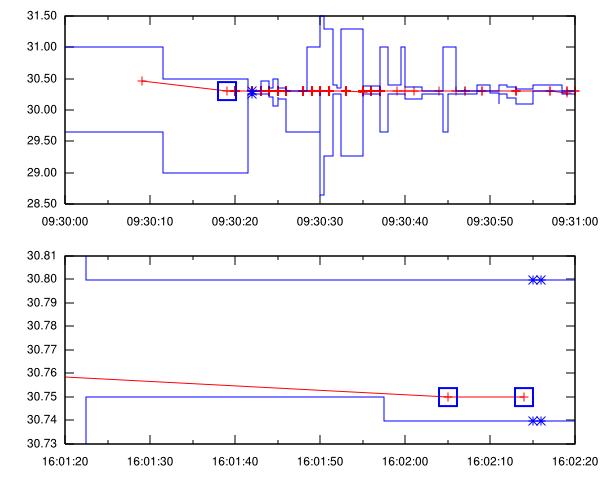
\includegraphics[width=0.7\linewidth]{gfx/m3l3_brownlees_fig4_open_close_minute.png}
\par\smallskip{\small \textbf{Hình 4:} Phút giao dịch đầu tiên và cuối cùng của cổ phiếu General Electric vào ngày 7 tháng 8 năm 2002. Mỗi dấu cộng trên đường giá giao dịch đánh dấu một giao dịch khác nhau. Các ô vuông trong bảng trên biểu thị giao dịch mở cửa của NYSE, còn các ô vuông trong bảng dưới biểu thị giao dịch đóng cửa của NYSE. Các dấu sao trên các đường giá chào mua-chào bán biểu thị báo giá mở cửa và đóng cửa của NYSE.}
\end{figure}

\noindent\textbf{Giá mở cửa và đóng cửa.} Một cách tự nhiên, người ta có thể kỳ vọng rằng giao dịch/báo giá đầu tiên (tương ứng, cuối cùng) trong ngày chính là giao dịch/báo giá mở cửa (tương ứng, đóng cửa) đã được ghi nhận chính thức. Tuy nhiên, từ Hình 4, thể hiện thời điểm đóng cửa và mở cửa của ngày giao dịch đang xét, có thể thấy rằng các giao dịch và báo giá đầu tiên trong ngày không phải là giao dịch và báo giá mở cửa chính thức của NYSE. Đáng chú ý là báo giá mở cửa cũng được ghi nhận sau giao dịch mở cửa. Vào thời điểm đóng cửa của NYSE trong cùng ngày đó, giao dịch cuối cùng được báo cáo trước 4:05 chiều thực sự là giao dịch đóng cửa, nhưng báo giá cuối cùng được báo cáo trong ngày lại không phải là báo giá đóng cửa. Do đó, việc xác định thời điểm mở cửa và đóng cửa của NYSE khó khăn hơn nhiều so với những gì người ta có thể nghĩ.

Ngày giao dịch chính thức của NYSE bắt đầu lúc 9:30 sáng và kết thúc lúc 4:00 chiều, nhưng trên thực tế, giao dịch sẽ bắt đầu muộn hơn một khoảng thời gian so với thời điểm mở cửa chính thức và tiếp tục kéo dài quá thời điểm đóng cửa, điều này hàm ý rằng thời điểm mở cửa và đóng cửa thực tế là ngẫu nhiên. Ngoài ra, rất thường gặp các báo cáo giao dịch và báo giá trong dữ liệu rõ ràng không thuộc về ngày giao dịch của NYSE, tức là các giao dịch trước 9:30 sáng và sau 4:00 chiều. Các bản ghi giao dịch và báo giá này có thể đến từ các sàn giao dịch khác hoặc từ các phiên giao dịch ngoài giờ (off-hours/crossing sessions) của NYSE, và do đó bị loại bỏ. Cuối cùng, để làm phức tạp thêm vấn đề, việc giao dịch thực tế của một cổ phiếu bắt đầu muộn hơn thời điểm mở cửa do độ trễ mở cửa (opening delays) không phải là điều hiếm gặp; ngoài ra, vào một số ngày đặc biệt (chẳng hạn những ngày trước kỳ nghỉ lễ), sàn giao dịch có thể đóng cửa sớm hơn.

Do đó, rất tiếc là không phải lúc nào cũng có thể xác định chính xác dữ liệu mở cửa và đóng cửa. Trường MODE trong dữ liệu báo giá (Bảng 1) cùng các trường G127 và COND trong dữ liệu giao dịch (Bảng 3) chứa một số cờ (flag) có thể dùng để xác định chính xác các giao dịch và báo giá mở cửa/đóng cửa, nhưng thông tin này không phải lúc nào cũng được báo cáo chính xác. Trên thực tế, giá giao dịch, giá chào mua hoặc giá chào bán đầu tiên và cuối cùng trong ngày không được kỳ vọng khác biệt đáng kể so với giá mở cửa và đóng cửa thực sự, và có thể được dùng làm biến đại diện (proxy). Tuy nhiên, điều này không đúng đối với khối lượng giao dịch và khối lượng báo giá.

Để nắm bắt đầy đủ mức giá đóng cửa trong ngày, chúng tôi áp dụng quy ước rằng khung giờ của ngày giao dịch trải dài từ 9:30 sáng đến 4:05 chiều. Quy ước này đảm bảo, ở mức độ lớn, rằng những mức giá đóng cửa được ghi nhận trễ cũng được tính đến. Khi sử dụng các khoảng thời gian cố định, chẳng hạn khi xây dựng chuỗi lợi suất 10 phút, khoảng thời gian cuối cùng trong ngày sẽ có độ dài danh nghĩa lớn hơn (trong ví dụ này là 15 phút, từ 3:50 chiều đến 4:05 chiều). Khi đó, lợi suất được tính bằng chênh lệch logarit (log-difference) giữa giá đóng cửa và mức giá ghi nhận lúc 3:50 chiều, coi là quan sát cuối cùng trong ngày.


% ---- Lesson 4: Singular Value Decomposition of Matrices ----
% Thứ tự đọc: Lesson Notes -> Đọc thêm
\chapter{Phân rã Giá trị Kỳ dị của Ma trận}
\label{ch:M3L4}

% Lesson: Singular Value Decomposition of Matrices

\section*{Lesson Notes}

MODULE 3 | BÀI 4

{\small
\begin{longtable}{>{\raggedright\arraybackslash}p{0.213\linewidth}>{\raggedright\arraybackslash}p{0.727\linewidth}}
\toprule
\textbf{Thời gian đọc} & 60 phút \\
\addlinespace[2pt]
\textbf{Kiến thức nền tảng} & Các phép toán ma trận cơ bản, đại số tuyến tính, Python cơ bản \\
\addlinespace[2pt]
\textbf{Từ khóa} & Phân rã giá trị kỳ dị (SVD), SVD đầy đủ và SVD cỡ kinh tế, xấp xỉ ma trận \\
\addlinespace[2pt]
\bottomrule
\end{longtable}
}

\emph{Trong bài học trước, chúng ta đã giới thiệu các phương pháp phân rã một ma trận đối xứng. Tuy nhiên, nhiều khi tập dữ liệu hay ma trận mà ta có lại không phải là ma trận đối xứng. Trong bài học này, chúng ta sẽ giới thiệu một phương pháp tổng quát để phân rã một ma trận. Phương pháp này được gọi là Phân rã Giá trị Kỳ dị, hay SVD. Chúng ta sẽ đi qua định nghĩa và các tính chất của SVD, sau đó trình bày một ứng dụng.}

\section{Giới thiệu Phân rã Giá trị Kỳ dị (SVD)}

\textbf{Phân rã giá trị kỳ dị (SVD)} là một phương pháp rất phổ biến trong đại số tuyến tính số. Phương pháp này thường được dùng để giải bài toán hồi quy tuyến tính khi ma trận không vuông. Nó cũng có thể được dùng như một phương pháp giảm chiều dữ liệu. Một ví dụ là dùng SVD làm cơ sở cho phân tích thành phần chính. SVD cũng là một phương pháp số nền tảng cho các thuật toán học máy.

Trong module trước, chúng ta đã thảo luận cách chéo hóa một ma trận đối xứng. Nếu $A$ là một ma trận đối xứng cỡ 3 nhân 3, ta có thể chéo hóa hay phân tích $A$ thành nhân tử như sau:

\[
A=\begin{bmatrix}
| & | &  |\\
v_{1} & v_{2} & v_{3} \\
| & | & |
\end{bmatrix}\begin{bmatrix}
\lambda_{1} & 0 & 0 \\
0 & \lambda_{2} & 0 \\
0 & 0 & \lambda_{3}
\end{bmatrix}\begin{bmatrix}
| & | &  |\\
v_{1} & v_{2} & v_{3} \\
| & | & |
\end{bmatrix}^{T}
\]

trong đó

$v_{1} , v_{2} , v_{3}$ là các vector riêng của $A$

$\lambda_{1} , \lambda_{2} , \lambda_{3}$ là các giá trị riêng của $A$

Tuy nhiên, phần lớn thời gian, các tập dữ liệu hay ma trận mà ta có sẽ không có tính đối xứng. Do đó, ta cần một phương pháp để chéo hóa một ma trận tổng quát. Phương pháp này chính là phân rã giá trị kỳ dị.

\section{Định nghĩa Phân rã Giá trị Kỳ dị}

\subsection{Biểu diễn Ma trận của SVD}

\textbf{Phân rã giá trị kỳ dị} là một phương pháp phân rã một ma trận thành ba ma trận. Với mọi ma trận $A$ cỡ $m\times n$ có các phần tử thực, tồn tại một phân tích thành nhân tử có dạng:

\[
A=U\Sigma V^{T}
\]

Trong đó:

$U$ là một ma trận unita và trực giao cỡ $m\times m$, do đó là ma trận trực chuẩn

$\Sigma$ là một ma trận đường chéo hình chữ nhật cỡ $m\times n$ với các số thực khác không trên đường chéo

$V^{T}$ là chuyển vị của $V$; $V$ là một ma trận unita và trực giao (trực chuẩn) cỡ $n\times n$

Ta cũng có thể viết lại công thức trên dưới dạng ma trận sau, với giả định $m\ge n$.

\[
\begin{bmatrix}
 &  &  &  \\
| & | &  & |\\
a_{1} & a_{2} & ... & a_{n} \\
| & | &  & |\\
 &  &  &
\end{bmatrix}=\begin{bmatrix}
 &  &  &  \\
| & | &  & |\\
u_{1} & u_{2} & ... & u_{m} \\
| & | &  & |\\
 &  &  &
\end{bmatrix}\begin{bmatrix}
\sigma_{1} & 0 & ... & 0 \\
0 & \sigma_{2} & ... & 0 \\
0 & 0 & ... & 0 \\
0 & 0 & ... & \sigma_{n} \\
0 & 0 & ... & 0
\end{bmatrix}\begin{bmatrix}
 &  &  &  \\
| & | & | & | \\
v_{1} & v_{2} & ... & v_{n} \\
| & | & | & | \\
 &  &  &
\end{bmatrix}^{T}
\]

trong đó $a$ là $n$ vector cột trong ma trận $A$, $u$ là $m$ vector cột trong ma trận $U$, và $v$ là $n$ vector cột trong ma trận $V$.

Các cỡ ma trận ở trên như sau:
\[
\left[ m\times n \right]=\left[ m\times m \right]\left[ m\times n \right]\left[ n\times n \right]
\]

Các phần tử đường chéo $\sigma_{i}$ của $\Sigma$ được gọi là các \textbf{giá trị kỳ dị} của $A$. Chúng thường được sắp xếp theo thứ tự giảm dần ($\sigma_{1} \geq \sigma_{2} \geq ... \geq \sigma_{\min(m,n)} \geq 0$). Vì ma trận $\Sigma$ ở trên giả định $m \ge n$, nên có tối đa $n$ giá trị kỳ dị dương. Giá trị của các hàng còn lại trong $\Sigma$ bằng 0.

Các vector trong ma trận $U$ được gọi là các \textbf{vector kỳ dị trái} của $A$.

Các vector trong ma trận $V$ được gọi là các \textbf{vector kỳ dị phải} của $A$.

\subsection{Diễn giải Hình học của Phân rã Giá trị Kỳ dị (SVD)}

SVD có thể được diễn giải về mặt hình học như một hợp của ba phép biến đổi:
\begin{enumerate}
  \item Một phép quay hoặc phản xạ $U$
  \item Một phép co giãn hoặc mở rộng dọc theo các trục tọa độ $\Sigma$
  \item Một phép quay hoặc phản xạ khác $V^{T}$
\end{enumerate}

Cách diễn giải này giúp hiểu SVD nắm bắt cấu trúc cốt lõi của các phép biến đổi tuyến tính như thế nào. Đồ thị sau minh họa phép phân rã.

\textbf{Hình 1: Minh họa Phân rã Giá trị Kỳ dị}

% [Hình chưa có trong gfx: images/FD_M3_L4_decomposition.jpg]
\begin{figure}[H]
\centering
\fbox{\parbox{0.9\linewidth}{\small \emph{[Hình minh họa: Sơ đồ mô tả quá trình Phân rã Giá trị Kỳ dị (SVD), cho thấy các phép biến đổi: một phép biến đổi tuyến tính (A), các phép quay (U và V$^{T}$), và phép co giãn ($\Sigma$), được biểu diễn trên mặt phẳng 2D cùng các vector.]}}}
\end{figure}

\section{Các Tính chất của Phân rã Giá trị Kỳ dị (SVD)}

Trong mục này, chúng ta sẽ thảo luận một số tính chất then chốt của SVD.

\subsubsection*{Tính chất 1.}

Vì các vector trong $U$ và $V$ là unita và trực giao,

$U^{T}U=UU^{T}=I_{m\times m}$ \quad (ma trận đơn vị)

$V^{T}V=VV^{T}=I_{n\times n}$ \quad (ma trận đơn vị)

\subsubsection*{Tính chất 2.}

Số giá trị kỳ dị khác không trong ma trận $\Sigma$ chính là hạng của ma trận $A$.

\subsubsection*{Tính chất 3.}

Vì các giá trị kỳ dị $\sigma$ được sắp xếp theo thứ tự giảm dần trong ma trận $\Sigma$, cột thứ nhất của $U$ (là $u_{1}$) và cột thứ nhất của $V$ (là $v_{1}$) tương ứng với $\sigma_{1}$ quan trọng hơn cột thứ hai của các ma trận $U$ và $V$ trong việc mô tả thông tin của ma trận $A$. Các cột thứ nhất của $U$ và $V$ cũng quan trọng hơn cột thứ ba trong việc mô tả ma trận $A$, và cứ tiếp tục như vậy. Do tính chất này, khi một số giá trị $\sigma$ rất nhỏ, điều đó có nghĩa là chúng chỉ chứa một lượng thông tin rất nhỏ của ma trận $A$. Ta có thể bỏ các $\sigma$ này cùng các cột tương ứng của chúng trong các ma trận $U$ và $V$.

\subsubsection*{Tính chất 4.}

Trong phần trước, chúng ta đã đề cập rằng số giá trị kỳ dị khác không trong ma trận $\Sigma$ là giá trị nhỏ nhất của $m$ và $n$. Do đó, có thể có các hàng toàn số $0$ ở phần dưới của ma trận $\Sigma$. Kết quả là, khi ta thực hiện tích vô hướng của ma trận $U$ với ma trận $\Sigma$, các vector tương ứng của $U$ sẽ nhân với tất cả các hàng số $0$ trong ma trận $\Sigma$ và cho kết quả bằng $0$. Từ kết quả này, ta có thể đơn giản hóa SVD về dạng rút gọn bằng cách bỏ các hàng toàn số $0$ trong ma trận $\Sigma$ và các vector tương ứng trong ma trận $U$. Hình 2 dưới đây minh họa tính chất này.

\textbf{Hình 2: SVD Đầy đủ so với SVD Cỡ kinh tế/Rút gọn}

Sơ đồ so sánh Phân rã Giá trị Kỳ dị (SVD) đầy đủ và cỡ kinh tế, cho thấy các ma trận $A$, $U$, $\Sigma$, và $V^T$ cùng các thành phần và số chiều tương ứng:

% [Hình chưa có trong gfx: images/FD_M3_L4_reduced_SVD.jpg]
\begin{figure}[H]
\centering
\fbox{\parbox{0.9\linewidth}{\small \emph{[Hình minh họa: Sơ đồ so sánh Phân rã Giá trị Kỳ dị (SVD) đầy đủ và rút gọn, cho thấy các ma trận A, U, $\Sigma$, và V$^{T}$ cùng các thành phần và số chiều tương ứng.]}}}
\end{figure}

Trong phương trình đầu tiên ở Hình 2, ta thấy khi thực hiện tích vô hướng của $U$ và $\Sigma$, phần $\hat{U}^{\bot }$ của $U$ sẽ nhân với các số $0$ của $\Sigma$. Kết quả sẽ bằng $0$. Do đó, ta có thể bỏ chúng đi mà không mất thông tin nào trong ma trận A. Phương trình thứ hai là dạng rút gọn của SVD. Dạng này được gọi là \textbf{SVD rút gọn} hay \textbf{SVD cỡ kinh tế}.

\section{Xấp xỉ Ma trận bằng SVD}

Trong mục này, chúng ta sẽ minh họa cách dùng SVD để xấp xỉ một ma trận. Đây là lý do phổ biến nhất để dùng SVD.

Giả sử với ma trận A cỡ $m \times n$, hạng là $r$, và $r<min(m,n)$. Ta có thể viết SVD của ma trận $A$ như sau.

\[
A=\begin{bmatrix}
 &  &  &  \\
| & | &  & |\\
a_{1} & a_{2} & ... & a_{n} \\
| & | &  & |\\
 &  &  & \\
 &  &  &
\end{bmatrix}=\begin{bmatrix}
 &  &  &  \\
| & | &  & |\\
u_{1} & u_{2} & ... & u_{m} \\
| & | &  & |\\
 &  &  & \\
 &  &  &
\end{bmatrix}\begin{bmatrix}
\sigma_{1} & 0 & ... & 0 &0 \\
0 & \sigma_{2} & ... & 0 &0\\
0 & 0 & ... & 0 &0\\
0 & 0 & ... & \sigma_{r} &0\\
0 & 0 & ... & 0 &0\\
0 & 0 & ... & 0 &0
\end{bmatrix}\begin{bmatrix}
 &  &  &  \\
| & | & | & | \\
v_{1} & v_{2} & ... & v_{n} \\
| & | & | & | \\
 &  &  & \\
 &  &  &
\end{bmatrix}^{T}
\]

Từ các giá trị kỳ dị trong $\Sigma$, ta biết $\sigma_{1}\ge \sigma_{2}\ge ...\ge \sigma_{r}>\sigma_{r+1}=...\sigma_{min(m,n)}=0$. Ta có thể khai triển ma trận A như sau.

\[
A=\sum_{k=1}^{r}\sigma_{k}u_{k}v_{k}^{T}=\sigma_{1}u_{1}v_{1}^{T}+\sigma_{2}u_{2}v_{2}^{T}+...+\sigma_{r-1}u_{r-1}v_{r-1}^{T}+\sigma_{r}u_{r}v_{r}^{T}
\]

Đây được gọi là định lý Eckart-Young. Theo định lý này, ta có thể biểu diễn ma trận $A$ chỉ bằng $r$ vector đầu tiên trong ma trận $U$ và $r$ vector đầu tiên trong ma trận $V$, vì trong ma trận $\Sigma$ chỉ có $r$ giá trị $\sigma$ khác không.

Ta cũng biết rằng các $\sigma$ trong $\Sigma$ được sắp xếp theo thứ tự giảm dần. Nếu các $\sigma$ ở vế phải của phương trình quá nhỏ, ta có thể bỏ chúng khỏi phương trình. Khi đó, ta có thể xấp xỉ ma trận $A$ chỉ bằng các $\sigma$ có giá trị lớn. Giả sử ta chỉ muốn giữ lại $\hat{r}$ giá trị $\sigma$ đầu tiên trong phương trình, trong đó $r \ge \hat{r}$. Ma trận $A$ xấp xỉ có thể được biểu diễn như sau.

\[
\tilde{A}=\sum_{k=1}^{\hat{r}}\sigma_{k}u_{k}v_{k}^{T}=\sigma_{1}u_{1}v_{1}^{T}+\sigma_{2}u_{2}v_{2}^{T}+...+\sigma_{\hat{r}-1}u_{\hat{r}-1}v_{\hat{r}-1}^{T}+\sigma_{\hat{r}}u_{\hat{r}}v_{\hat{r}}^{T}
\]

$\tilde{A}$ là xấp xỉ của A. Dựa trên phương trình và phần giải thích ở trên, $\tilde{A}$ chứa ít điểm dữ liệu hơn $A$ nhưng vẫn giữ phần lớn thông tin từ ma trận gốc $A$. Ta giảm chiều dữ liệu bằng cách dùng SVD để xấp xỉ một ma trận. Điều này nhờ vào tính chất của SVD cho phép ta giải các bài toán bình phương tối thiểu hoặc chạy các thuật toán học máy hiệu quả hơn.

\section{Ứng dụng của Phân rã Giá trị Kỳ dị (SVD)}

Trong mục này, chúng ta sẽ dùng một số dữ liệu tài chính để minh họa cách sử dụng SVD. Chúng ta sẽ dùng dữ liệu giá cổ phiếu của Apple, Ford Motor, Pfizer và Walmart để cho thấy cách áp dụng SVD. Trước hết, hãy tải một số thư viện Python cho ứng dụng này.

\begin{lstlisting}[language=Python,escapeinside={(*@}{@*)}]
import datetime
import math
import matplotlib.pyplot as plt
import numpy as np
import pandas as pd
import seaborn as sns
import yfinance as yfin

from numpy import linalg as LA
\end{lstlisting}

\subsection{Nhập Dữ liệu}

Tiếp theo, chúng ta sẽ tải dữ liệu giá cổ phiếu từ Yahoo Finance.

\begin{lstlisting}[language=Python,escapeinside={(*@}{@*)}]
# (*@Tải@*) (*@giá@*) (*@cổ@*) (*@phiếu@*) (*@từ@*) Yahoo Finance (*@và@*) (*@đặt@*) (*@khoảng@*) (*@thời@*) gian (*@tải@*) (*@về@*)
start = datetime.date(2018, 1, 2)
end = datetime.date(2023, 12, 31)

# (*@Lấy@*) (*@dữ@*) (*@liệu@*)
# (*@Để@*) (*@chuyển@*) (*@đổi@*) (*@giữa@*) (*@tải@*) (*@dữ@*) (*@liệu@*) (*@trực@*) (*@tiếp@*) (*@và@*) (*@nạp@*) (*@dữ@*) (*@liệu@*) (*@cục@*) (*@bộ,@*) 
# (*@bỏ@*) (*@dấu@*) (*@chú@*) (*@thích@*) (*@ở@*) (*@dòng@*) mong (*@muốn@*) (*@và@*) (*@chú@*) (*@thích@*) (*@dòng@*) (*@còn@*) (*@lại.@*)
# (*@Lấy@*) (*@dữ@*) (*@liệu@*) Amazon, Ford (*@và@*) Bitcoin
#stocks = yfin.download(["AAPL", "F", "WMT","PFE"], start, end, auto_adjust = False)["Adj Close"]
stocks = pd.read_csv('FD_M3_L4_stocks.csv', index_col='Date', parse_dates=True)\
                    .loc[start:end].reindex(columns=["AAPL", "F", "WMT","PFE"])

stocks.head()
\end{lstlisting}

\begin{lstlisting}[escapeinside={(*@}{@*)}]
                 AAPL         F        WMT        PFE
Date                                                 
2018-01-02  40.341885  8.263117  28.914423  24.229599
2018-01-03  40.334858  8.328384  29.166639  24.409126
2018-01-04  40.522213  8.471978  29.193027  24.462317
2018-01-05  40.983566  8.615572  29.366074  24.508865
2018-01-08  40.831348  8.582937  29.800114  24.236256
\end{lstlisting}

\begin{lstlisting}[language=Python,escapeinside={(*@}{@*)}]
stocks.index = pd.to_datetime(stocks.index).strftime("%Y-%m-%d")
\end{lstlisting}

\subsection{Tính Lợi suất}

Bây giờ, hãy tính lợi suất của các giá cổ phiếu này.

\begin{lstlisting}[language=Python,escapeinside={(*@}{@*)}]
# (*@Để@*) (*@tính@*) (*@lợi@*) (*@suất@*) (*@của@*) (*@các@*) (*@cổ@*) (*@phiếu,@*) ta (*@cần@*) (*@loại@*) (*@bỏ@*) (*@các@*) (*@hàng@*) NA.
stocks_returns = stocks[["AAPL", "F", "WMT","PFE"]].dropna().pct_change()
stocks_returns = stocks_returns.dropna()
stocks_returns.head()
\end{lstlisting}

\begin{lstlisting}[escapeinside={(*@}{@*)}]
                AAPL         F       WMT       PFE
Date                                              
2018-01-03 -0.000174  0.007899  0.008723  0.007409
2018-01-04  0.004645  0.017241  0.000905  0.002179
2018-01-05  0.011385  0.016949  0.005928  0.001903
2018-01-08 -0.003714 -0.003788  0.014780 -0.011123
2018-01-09 -0.000115 -0.005323 -0.012007 -0.001098
\end{lstlisting}

\subsection{Tính SVD}

Bây giờ chúng ta đã có tập dữ liệu lợi suất giá cổ phiếu của bốn cổ phiếu. Ta có thể tính SVD một cách đơn giản bằng hàm Python sau.

\begin{lstlisting}[language=Python,escapeinside={(*@}{@*)}]
# (*@Thực@*) (*@hiện@*) SVD cho (*@lợi@*) (*@suất@*) (*@cổ@*) (*@phiếu@*)
U, s, VT = np.linalg.svd(stocks_returns)
\end{lstlisting}

\begin{lstlisting}[language=Python,escapeinside={(*@}{@*)}]
# (*@Trình@*) (*@bày@*) (*@kết@*) (*@quả@*)
print("Stock Returns Matrix Dimension:")
print(stocks_returns.shape)
print("\nDimension of Matrix U:")
print(U.shape)
print("\nSingular values:")
print(s)
print("\nDimension of Matrix V^T:")
print(VT.shape)
\end{lstlisting}

\begin{lstlisting}[escapeinside={(*@}{@*)}]
Stock Returns Matrix Dimension:
(1508, 4)

Dimension of Matrix U:
(1508, 1508)

Singular values:
[1.11696739 0.72489554 0.55820564 0.47159228]

Dimension of Matrix V^T:
(4, 4)

\end{lstlisting}

\section{So sánh PCA và SVD}

Cho đến nay, việc tính SVD của một ma trận bằng Python rất đơn giản. Hãy làm cho mọi thứ thú vị hơn một chút. Chúng ta sẽ cho thấy mối liên hệ giữa SVD và phân tích thành phần chính (PCA) (Brunton et al.).

Trong Module 1, chúng ta đã thảo luận ngắn gọn cách thu được các thành phần chính bằng vector riêng và giá trị riêng. Trong mục này, chúng ta sẽ chỉ cho bạn cách dùng SVD của một ma trận để thu được giá trị riêng và vector riêng.

Hãy nhớ rằng trong Module 2, trước khi đi đến các thành phần chính, ta cần chuẩn hóa dữ liệu. Hãy làm điều đó trước.

\begin{lstlisting}[language=Python,escapeinside={(*@}{@*)}]
# (*@Chuẩn@*) (*@hóa@*) (*@tập@*) (*@dữ@*) (*@liệu@*) (*@lợi@*) (*@suất@*) (*@cổ@*) (*@phiếu@*)
stocks_returns_means = stocks_returns.mean()
stocks_returns_stds = stocks_returns.std()
standardized_returns = (stocks_returns - stocks_returns_means) / stocks_returns_stds
standardized_returns.head()
\end{lstlisting}

\begin{lstlisting}[escapeinside={(*@}{@*)}]
                AAPL         F       WMT       PFE
Date                                              
2018-01-03 -0.070358  0.286261  0.584133  0.446787
2018-01-04  0.171148  0.647641  0.029986  0.124438
2018-01-05  0.508925  0.636338  0.386009  0.107413
2018-01-08 -0.247757 -0.165773  1.013486 -0.695380
2018-01-09 -0.067374 -0.225159 -0.885164 -0.077534
\end{lstlisting}

Tiếp theo, ta muốn tính hiệp phương sai của ma trận lợi suất đã chuẩn hóa. Dạng ma trận của phương trình hiệp phương sai như sau.

\[
\left( \frac{\text{ma trận lợi suất chuẩn hóa}}{\sqrt{n-1}} \right)^{T}\bullet \left( \frac{\text{ma trận lợi suất chuẩn hóa}}{\sqrt{n-1}} \right)
\]

\begin{lstlisting}[language=Python,escapeinside={(*@}{@*)}]
# (*@Tính@*) (*@hiệp@*) (*@phương@*) sai cho ma (*@trận@*) (*@lợi@*) (*@suất@*) (*@chuẩn@*) (*@hóa@*)
standardized_returns_dvd_sqrt_n=(standardized_returns/math.sqrt(len(standardized_returns)-1))
standardized_returns_cov = standardized_returns_dvd_sqrt_n.T@standardized_returns_dvd_sqrt_n
standardized_returns_cov
\end{lstlisting}

\begin{lstlisting}[escapeinside={(*@}{@*)}]
          AAPL         F       WMT       PFE
AAPL  1.000000  0.376460  0.365246  0.324438
F     0.376460  1.000000  0.185248  0.224384
WMT   0.365246  0.185248  1.000000  0.296375
PFE   0.324438  0.224384  0.296375  1.000000
\end{lstlisting}

Bây giờ, hãy thực hiện một số phép biến đổi ma trận đơn giản trên hiệp phương sai của lợi suất chuẩn hóa. Giả sử ma trận $B$ là $\left( \frac{\text{ma trận lợi suất chuẩn hóa}}{\sqrt{n-1}} \right)$. Do đó, ta có thể viết lại hiệp phương sai của lợi suất chuẩn hóa như sau.

\[
\text{Hiệp phương sai} = B^{T}B
\]

Với SVD, ta có thể viết ma trận $B$ là $B=U\Sigma V^{T}$. Khi đó, chuyển vị của nó là $B^{T}=V\Sigma U^{T}$. Sau đó, ta có thể tính hiệp phương sai của lợi suất chuẩn hóa như sau.

\[
\text{Hiệp phương sai} =B^{T}B=V\Sigma U^{T}U\Sigma V^{T}=V\Sigma\Sigma V^{T}=V\Sigma^{2} V^{T}
\]

Vì tính chất $U^{T}U=I$ là ma trận đơn vị, ta có thể bỏ $U^{T}U$. Tiếp theo, hãy thực hiện phép tính sau.

\[
B^{T}BV=V\Sigma^{2} V^{T}V=V\Sigma^{2}
\]

Ta có thể bỏ $V^{T}V$ vì $V^{T}V=I$ là ma trận đơn vị. Phương trình trên có gợi cho bạn điều gì không? Đúng vậy, phương trình cho thấy các vector cột trong ma trận $V$ là các vector riêng của $B^{T}B$. Các giá trị kỳ dị bình phương trong ma trận $\Sigma$ là các giá trị riêng của $B^{T}B$. Do đó, $Bv_{1}$ là thành phần chính thứ nhất và $\sigma_{1}^{2}$ tương ứng là phương sai của tập dữ liệu $B$ được giải thích bởi thành phần chính thứ nhất.

Bây giờ, bạn thực ra có hai cách để tính các thành phần chính. Phương pháp thứ nhất, như đã mô tả ở Module 1, Bài 4, là tính các giá trị riêng và vector riêng của ma trận hiệp phương sai của dữ liệu. Phương pháp thứ hai là tính SVD của dữ liệu. Khi đó, ma trận $V$ sẽ chứa các vector riêng, và các giá trị kỳ dị bình phương sẽ là các giá trị riêng.

Bây giờ hãy thử cả hai phương pháp để thu được giá trị riêng và vector riêng.

\begin{lstlisting}[language=Python,escapeinside={(*@}{@*)}]
# (*@Dùng@*) SVD (*@để@*) (*@tính@*) vector (*@riêng@*) (*@và@*) (*@giá@*) (*@trị@*) (*@riêng@*) (*@của@*) ma (*@trận@*) (*@hiệp@*) (*@phương@*) sai (*@của@*) (*@lợi@*) (*@suất@*) (*@chuẩn@*) (*@hóa@*)
U_st_return, s_st_return, VT_st_return = np.linalg.svd(standardized_returns_dvd_sqrt_n)
print("\nSquared Singular values (eigenvalues):")
print(s_st_return**2)
print("\nMatrix V (eigenvectors)")
print(VT_st_return.T)
\end{lstlisting}

\begin{lstlisting}[escapeinside={(*@}{@*)}]

Squared Singular values (eigenvalues):
[1.8947492  0.83555338 0.71064931 0.55904811]

Matrix V (eigenvectors)
[[ 0.56634769  0.14011624 -0.21637439 -0.78281534]
 [ 0.45964766  0.75759291  0.0183351   0.46307756]
 [ 0.48586769 -0.53226779 -0.55857187  0.41063494]
 [ 0.48156713 -0.35087237  0.80052696  0.06432933]]

\end{lstlisting}

\begin{lstlisting}[language=Python,escapeinside={(*@}{@*)}]
# (*@Dùng@*) (*@phương@*) (*@pháp@*) (*@từ@*) Module 1 (*@Bài@*) 4 (*@để@*) (*@tính@*) vector (*@riêng@*) (*@và@*) 
# (*@giá@*) (*@trị@*) (*@riêng@*) (*@của@*) ma (*@trận@*) (*@hiệp@*) (*@phương@*) sai (*@của@*) (*@lợi@*) (*@suất@*) (*@chuẩn@*) (*@hóa@*)
eigenvalues, eigenvectors = LA.eig(standardized_returns_cov)
idx = np.argsort(eigenvalues)[::-1]
eigenvalues = eigenvalues[idx]
eigenvectors = eigenvectors[:, idx]
eigenvalues
\end{lstlisting}

\begin{lstlisting}[escapeinside={(*@}{@*)}]
array([1.8947492 , 0.83555338, 0.71064931, 0.55904811])
\end{lstlisting}

\begin{lstlisting}[language=Python,escapeinside={(*@}{@*)}]
eigenvectors
\end{lstlisting}

\begin{lstlisting}[escapeinside={(*@}{@*)}]
array([[-0.56634769,  0.14011624, -0.21637439, -0.78281534],
       [-0.45964766,  0.75759291,  0.0183351 ,  0.46307756],
       [-0.48586769, -0.53226779, -0.55857187,  0.41063494],
       [-0.48156713, -0.35087237,  0.80052696,  0.06432933]])
\end{lstlisting}

Từ kết quả trên, ta thấy cả hai phương pháp đều cho cùng các giá trị riêng. Cả hai phương pháp cũng cho cùng các vector riêng, ngoại trừ vector đầu tiên. Nhìn kỹ, ta thấy chúng chỉ khác nhau về dấu âm. Với vector riêng, chúng thực chất là như nhau vì dấu âm không làm thay đổi hướng hay độ lớn của cả hai vector riêng.

Bạn có thể dùng một trong hai phương pháp để thu được các vector riêng và giá trị riêng của một ma trận hiệp phương sai. Không có sự đồng thuận về việc phương pháp nào tốt hơn. Chúng ta thường dùng SVD để triển khai PCA, nén ảnh và các hệ thống gợi ý. Chúng ta sẽ dùng phương pháp trong Module 1, Bài 4 để giải các bài toán bình phương tối thiểu.

Một khác biệt then chốt giữa PCA và SVD là cách chúng xử lý điểm xuất phát. Nói chung, PCA làm việc trên ma trận hiệp phương sai hoặc ma trận tương quan. PCA cũng chuẩn hóa ma trận dữ liệu. Tuy nhiên, SVD có thể làm việc trực tiếp trên ma trận dữ liệu. Nếu SVD không chuẩn hóa ma trận dữ liệu, các giá trị riêng thu được có thể khác với các giá trị riêng tính từ PCA.

\section{Kết luận}

Trong bài học này, trước hết chúng ta đã giới thiệu SVD. Chúng ta đã nêu định nghĩa của nó, minh họa cách diễn giải hình học, và thảo luận các tính chất của nó. Sau đó, chúng ta đã trình bày ứng dụng của nó bằng Python. Chúng ta đã cho thấy cách dùng SVD để tính các giá trị riêng và vector riêng của một ma trận hiệp phương sai. Chúng ta cũng đã chỉ ra mối liên hệ giữa SVD và PCA.

\textbf{Tài liệu tham khảo}

\begin{itemize}
  \item Brunton, Steven L., et al. ``Chapter 1: Singular Value Decomposition (SVD) and Principal Components Analysis (PCA).'' University of Washington, 2015, \url{https://faculty.washington.edu/sbrunton/me565/pdf/CHAPTER1.pdf}.
\end{itemize}

\chapter{Đọc thêm 1: Phân rã Giá trị Kỳ dị (SVD) (Murphy)}
\label{ch:M3L4DT1}

% Nguồn: Murphy, K. P. ``Probabilistic Machine Learning: An Introduction.'' MIT Press, 2022, Sections 7.5.1-7.5.2, tr. 259-261.
% Phần cần đọc: Sections 7.5.1 (Basics), 7.5.2 (Connection Between SVD and EVD)
% Nội dung bắt buộc đọc: được kiểm tra trong mọi bài đánh giá (kể cả Quiz).

\section{Thông tin nguồn}

\begin{itemize}
  \item \textbf{Nguồn:} Murphy, Kevin Patrick. \emph{Probabilistic Machine Learning: An Introduction}. MIT Press, 2022. \url{https://probml.github.io/pml-book/book1.html}
  \item \textbf{Phần cần đọc:} Sections 7.5.1-7.5.2 (tr. 259-261)
\end{itemize}

\section{7.5 Phân rã Giá trị Kỳ dị (SVD)}

Bây giờ ta bàn về SVD, phép phân rã tổng quát hóa phân rã giá trị riêng (EVD) cho các ma trận chữ nhật.

\subsection{7.5.1 Cơ bản}

Bất kỳ ma trận (thực) $m \times n$ nào $\mathbf{A}$ đều có thể được phân rã thành

\begin{equation}
\mathbf{A} = \mathbf{U}\mathbf{S}\mathbf{V}^{\mathsf{T}} = \sigma_1 \begin{pmatrix} | \\ \boldsymbol{u}_1 \\ | \end{pmatrix} \begin{pmatrix} - & \boldsymbol{v}_1^{\mathsf{T}} & - \end{pmatrix} + \cdots + \sigma_r \begin{pmatrix} | \\ \boldsymbol{u}_r \\ | \end{pmatrix} \begin{pmatrix} - & \boldsymbol{v}_r^{\mathsf{T}} & - \end{pmatrix}
\tag{7.178}
\end{equation}

trong đó $\mathbf{U}$ là một ma trận $m \times m$ có các cột trực chuẩn (nên $\mathbf{U}^{\mathsf{T}}\mathbf{U} = \mathbf{I}_m$), $\mathbf{V}$ là một ma trận $n \times n$ có các hàng và cột trực chuẩn (nên $\mathbf{V}^{\mathsf{T}}\mathbf{V} = \mathbf{V}\mathbf{V}^{\mathsf{T}} = \mathbf{I}_n$), và $\mathbf{S}$ là một ma trận $m \times n$ chứa $r = \min(m,n)$ \textbf{giá trị kỳ dị} $\sigma_i \geq 0$ nằm trên đường chéo chính, với các phần còn lại được lấp đầy bằng 0. Các cột của $\mathbf{U}$ là các \textbf{vector kỳ dị trái}, và các cột của $\mathbf{V}$ là các vector kỳ dị phải. Phép phân rã này được gọi là \textbf{phân rã giá trị kỳ dị} hay \textbf{SVD} của ma trận. Xem Hình 7.8 để có một ví dụ minh họa.

\begin{figure}[H]
\centering
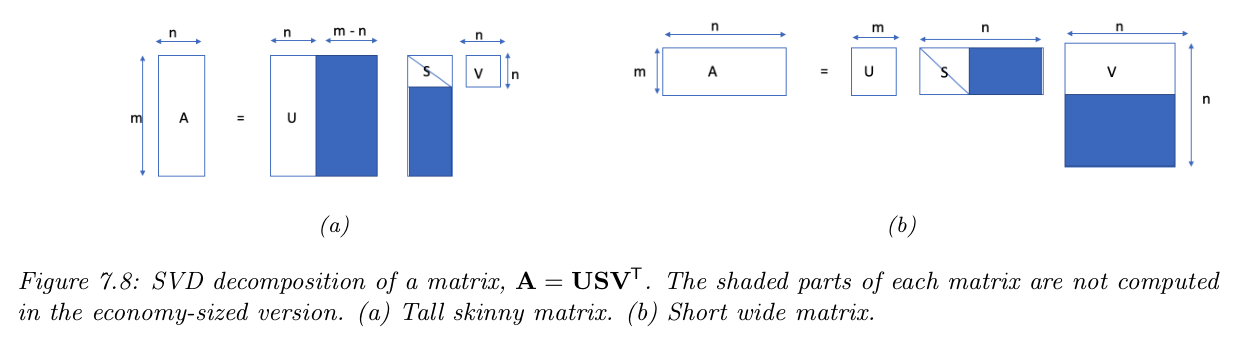
\includegraphics[width=0.85\linewidth]{gfx/m3l4_murphy_fig7-8_svd_decomposition.png}
\par\smallskip{\small \textbf{Hình 7.8:} Phân rã SVD của một ma trận, $\mathbf{A} = \mathbf{U}\mathbf{S}\mathbf{V}^{\mathsf{T}}$. Các phần tô bóng trong mỗi ma trận không được tính trong phiên bản SVD cỡ kinh tế. (a) Ma trận cao gầy. (b) Ma trận rộng thấp.}
\end{figure}

Như có thể thấy từ Hình 7.8a, nếu $m > n$, sẽ có tối đa $n$ giá trị kỳ dị, do đó $m - n$ cột cuối cùng của $\mathbf{U}$ không liên quan (vì chúng sẽ bị nhân với 0). Nếu ta viết ma trận $\mathbf{U}$ dưới dạng $\mathbf{U} = [\mathbf{U}_1, \mathbf{U}_2]$, ta chỉ cần tính $\mathbf{U}_1$. \textbf{SVD cỡ kinh tế} (economy sized SVD), còn gọi là \textbf{thin SVD}, tránh phải tính các phần tử không cần thiết đó. Hình 7.8b cho thấy trường hợp ngược lại, khi $m < n$, trong đó ta biểu diễn $\mathbf{V} = [\mathbf{V}_1; \mathbf{V}_2]$, và chỉ cần tính $\mathbf{V}_1$.

Chi phí tính toán SVD là $O(\min(mn^2, m^2n))$. Bạn đọc có thể tìm chi tiết về cách SVD hoạt động trong các giáo trình đại số tuyến tính chuẩn.

\subsection{7.5.2 Mối liên hệ giữa SVD và EVD}

Nếu $\mathbf{A}$ là thực, đối xứng và xác định dương, thì các giá trị kỳ dị bằng với các giá trị riêng, và các vector kỳ dị trái và phải bằng với các vector riêng (sai khác một dấu):

\begin{equation}
\mathbf{A} = \mathbf{U}\mathbf{S}\mathbf{V}^{\mathsf{T}} = \mathbf{U}\mathbf{S}\mathbf{U}^{\mathsf{T}} = \mathbf{U}\mathbf{S}\mathbf{U}^{-1}
\tag{7.179}
\end{equation}

Tuy nhiên, lưu ý rằng NumPy luôn trả về các giá trị kỳ dị theo thứ tự giảm dần, trong khi các giá trị riêng không nhất thiết được sắp xếp.

Nói chung, đối với một ma trận thực bất kỳ $\mathbf{A}$, nếu $\mathbf{A} = \mathbf{U}\mathbf{S}\mathbf{V}^{\mathsf{T}}$, ta có

\begin{equation}
\mathbf{A}^{\mathsf{T}}\mathbf{A} = \mathbf{V}\mathbf{S}^{\mathsf{T}}\mathbf{U}^{\mathsf{T}}\mathbf{U}\mathbf{S}\mathbf{V}^{\mathsf{T}} = \mathbf{V}(\mathbf{S}^{\mathsf{T}}\mathbf{S})\mathbf{V}^{\mathsf{T}}
\tag{7.180}
\end{equation}

Do đó

\begin{equation}
(\mathbf{A}^{\mathsf{T}}\mathbf{A})\mathbf{V} = \mathbf{V}\mathbf{D}_n
\tag{7.181}
\end{equation}

nên các vector riêng của $\mathbf{A}^{\mathsf{T}}\mathbf{A}$ bằng với $\mathbf{V}$, các vector kỳ dị phải của $\mathbf{A}$, và các giá trị riêng của $\mathbf{A}^{\mathsf{T}}\mathbf{A}$ bằng với $\mathbf{D}_n = \mathbf{S}^{\mathsf{T}}\mathbf{S}$, là một ma trận đường chéo $n \times n$ chứa bình phương các giá trị kỳ dị. Tương tự, ta có

\begin{equation}
\mathbf{A}\mathbf{A}^{\mathsf{T}} = \mathbf{U}\mathbf{S}\mathbf{V}^{\mathsf{T}}\mathbf{V}\mathbf{S}^{\mathsf{T}}\mathbf{U}^{\mathsf{T}} = \mathbf{U}(\mathbf{S}\mathbf{S}^{\mathsf{T}})\mathbf{U}^{\mathsf{T}}
\tag{7.182}
\end{equation}

\begin{equation}
(\mathbf{A}\mathbf{A}^{\mathsf{T}})\mathbf{U} = \mathbf{U}\mathbf{D}_m
\tag{7.183}
\end{equation}

nên các vector riêng của $\mathbf{A}\mathbf{A}^{\mathsf{T}}$ bằng với $\mathbf{U}$, các vector kỳ dị trái của $\mathbf{A}$, và các giá trị riêng của $\mathbf{A}\mathbf{A}^{\mathsf{T}}$ bằng với $\mathbf{D}_m = \mathbf{S}\mathbf{S}^{\mathsf{T}}$, là một ma trận đường chéo $m \times m$ chứa bình phương các giá trị kỳ dị. Tóm lại,

\begin{equation}
\mathbf{U} = \operatorname{evec}(\mathbf{A}\mathbf{A}^{\mathsf{T}}), \quad \mathbf{V} = \operatorname{evec}(\mathbf{A}^{\mathsf{T}}\mathbf{A}), \quad \mathbf{D}_m = \operatorname{eval}(\mathbf{A}\mathbf{A}^{\mathsf{T}}), \quad \mathbf{D}_n = \operatorname{eval}(\mathbf{A}^{\mathsf{T}}\mathbf{A})
\tag{7.184}
\end{equation}

Nếu ta chỉ dùng phần đã tính (khác 0) trong SVD cỡ kinh tế, ta có thể định nghĩa

\begin{equation}
\mathbf{D} = \mathbf{S}^2 = \mathbf{S}^{\mathsf{T}}\mathbf{S} = \mathbf{S}\mathbf{S}^{\mathsf{T}}
\tag{7.185}
\end{equation}

Cũng lưu ý rằng EVD không phải lúc nào cũng tồn tại, ngay cả với $\mathbf{A}$ vuông, trong khi SVD luôn tồn tại.


% ============ MODULE 4: ALTERNATIVE DATA ============

% ---- Lesson 1 ----
% Thứ tự đọc: Lesson Notes -> Đọc thêm
\chapter{Các Thước đo Độ tương đồng}
\label{ch:M4L1}

% Lesson: Similarity Measures

\section*{Lesson Notes}

MODULE 4 | BÀI 1

{\small
\begin{longtable}{>{\raggedright\arraybackslash}p{0.213\linewidth}>{\raggedright\arraybackslash}p{0.727\linewidth}}
\toprule
\textbf{Thời gian đọc} & 45 phút \\
\addlinespace[2pt]
\textbf{Kiến thức nền tảng} & Thống kê cơ bản: quen thuộc với các khái niệm như trung bình, độ lệch chuẩn, tương quan và các phân phối. Đại số tuyến tính: kiến thức cơ bản về vectơ, ma trận và các phép toán như tích vô hướng. Xác suất: hiểu biết cơ bản về các khái niệm xác suất để diễn giải các thước đo thống kê và ý nghĩa của chúng. Kiến thức tài chính và đầu tư: hiểu biết cơ bản về thị trường tài chính, các công cụ và chiến lược đầu tư; quen thuộc với các khái niệm đánh giá và quản trị rủi ro; kiến thức cơ bản về phân tích cảm xúc (sentiment analysis) và vai trò của nó trong việc hiểu xu hướng thị trường. \\
\addlinespace[2pt]
\textbf{Từ khóa} & Khoảng cách Euclid, khoảng cách Manhattan, độ tương đồng cosine, chỉ số Jaccard, Word Mover's Distance (WMD), Dynamic Time Warping, tương quan Pearson, tương quan hạng Spearman, Term Frequency-Inverse Document Frequency (TF-IDF), phân tích văn bản, xử lý ngôn ngữ tự nhiên (NLP), truy xuất thông tin \\
\addlinespace[2pt]
\bottomrule
\end{longtable}
}

\emph{Trong bài học này, chúng ta khám phá các thước đo độ tương đồng và cách sử dụng chúng trong thị trường tài chính, đặc biệt là Term Frequency-Inverse Document Frequency (TF-IDF) để phân tích dữ liệu văn bản như tin tức và mạng xã hội nhằm thu được hiểu biết phục vụ các quyết định đầu tư. Chúng ta sẽ đề cập các loại thước đo độ tương đồng khác nhau, những lợi ích của TF-IDF, cùng các ứng dụng của nó trong phân tích cảm xúc, quản trị rủi ro và các chiến lược đầu tư khác.}

\begin{lstlisting}[language=Python,escapeinside={(*@}{@*)}]
# (*@Tải@*) (*@các@*) (*@thư@*) (*@viện@*)
import numpy as np
import pandas as pd

from sklearn.feature_extraction.text import TfidfVectorizer
\end{lstlisting}

\section{1 Các Thước đo Độ tương đồng}

Các thước đo độ tương đồng là những phương pháp dùng để định lượng mức độ giống nhau giữa hai đối tượng dữ liệu. Chúng thiết yếu trong nhiều lĩnh vực, bao gồm khai phá dữ liệu, học máy và truy xuất thông tin. Việc lựa chọn thước đo độ tương đồng phụ thuộc vào loại dữ liệu và cách diễn giải mong muốn về độ tương đồng. Các loại thước đo độ tương đồng phổ biến gồm:

\textbf{Các thước đo khoảng cách:} Những thước đo này định lượng độ khác biệt. Khoảng cách càng nhỏ thì độ tương đồng càng cao:

\begin{itemize}
  \item Khoảng cách Euclid
  \item Khoảng cách Manhattan
  \item Khoảng cách Minkowski
  \item Word Mover's Distance (WMD)
  \item Dynamic Time Warping
\end{itemize}

\textbf{Các hệ số tương đồng:} Những thước đo này định lượng trực tiếp độ tương đồng. Giá trị càng cao thì độ tương đồng càng lớn:

\begin{itemize}
  \item Độ tương đồng cosine
  \item Chỉ số Jaccard
  \item Hệ số tương quan Pearson
  \item Tương quan hạng Spearman
\end{itemize}

Dưới đây chúng ta sẽ xem xét từng thước đo chi tiết hơn.

\subsection{1.1 Các Thước đo Khoảng cách}

\textbf{1. Khoảng cách Euclid}

\begin{itemize}
  \item \textbf{Loại:} Thước đo khoảng cách
  \item \textbf{Kiểu dữ liệu:} Dữ liệu số
  \item \textbf{Mô tả:} Đo khoảng cách đường thẳng giữa hai điểm trong không gian Euclid.
  \item \textbf{Công thức:} $\sqrt{\sum (x_i - y_i)^2}$ (trong đó $x$ và $y$ là các điểm dữ liệu, và $i$ biểu thị các chiều)
  \item \textbf{Diễn giải:} Khoảng cách càng nhỏ = độ tương đồng càng cao
  \item \textbf{Các trường hợp sử dụng:}
  \begin{itemize}
    \item Phân cụm K-means
    \item K láng giềng gần nhất (K-nearest neighbors)
    \item Tìm các điểm dữ liệu tương tự
  \end{itemize}
\end{itemize}

\textbf{2. Khoảng cách Manhattan}

\begin{itemize}
  \item \textbf{Loại:} Thước đo khoảng cách
  \item \textbf{Kiểu dữ liệu:} Dữ liệu số
  \item \textbf{Mô tả:} Đo khoảng cách giữa hai điểm bằng cách cộng các chênh lệch tuyệt đối của tọa độ. Còn được gọi là khoảng cách khối phố (city block distance) hay khoảng cách L1.
  \item \textbf{Công thức:} $\sum |x_i - y_i|$
  \item Diễn giải: Khoảng cách càng nhỏ = độ tương đồng càng cao
  \item \textbf{Các trường hợp sử dụng:}
  \begin{itemize}
    \item Hệ thống gợi ý
    \item Lựa chọn đặc trưng
    \item Bền vững trước các giá trị ngoại lai
  \end{itemize}
\end{itemize}

\textbf{3. Khoảng cách Minkowski}

\begin{itemize}
  \item \textbf{Loại:} Thước đo khoảng cách
  \item \textbf{Kiểu dữ liệu:} Dữ liệu số
  \item \textbf{Mô tả:} Một thước đo khoảng cách tổng quát bao gồm khoảng cách Euclid và khoảng cách Manhattan như các trường hợp đặc biệt.
  \item \textbf{Công thức:} $(\sum |x_i - y_i|^p)^{(1/p)}$ (trong đó $p$ là bậc của khoảng cách)
  \begin{itemize}
    \item $p = 1$: khoảng cách Manhattan
    \item $p = 2$: khoảng cách Euclid
  \end{itemize}
  \item \textbf{Diễn giải:} Khoảng cách càng nhỏ = độ tương đồng càng cao
  \item \textbf{Các trường hợp sử dụng:}
  \begin{itemize}
    \item Thích ứng với các phân phối dữ liệu khác nhau
    \item Thử nghiệm với các thước đo khoảng cách khác nhau
  \end{itemize}
\end{itemize}

\textbf{4. Word Mover's Distance (WMD)}

\begin{itemize}
  \item \textbf{Loại:} Thước đo khoảng cách
  \item \textbf{Kiểu dữ liệu:} Dữ liệu văn bản (tài liệu, câu)
  \item \textbf{Mô tả:} Đo độ khác biệt giữa hai tài liệu văn bản dựa trên ``chi phí di chuyển'' của các từ từ tài liệu này để khớp với các từ trong tài liệu kia. Sử dụng các embedding từ để biểu diễn từ trong một không gian ngữ nghĩa.
  \item \textbf{Diễn giải:} WMD càng thấp thì độ tương đồng càng cao.
  \item \textbf{Các trường hợp sử dụng:}
  \begin{itemize}
    \item Phân loại tài liệu
    \item Các tác vụ về độ tương đồng văn bản mà ý nghĩa ngữ nghĩa là quan trọng
    \item Phân cụm tài liệu
  \end{itemize}
\end{itemize}

\textbf{5. Dynamic Time Warping}

\begin{itemize}
  \item \textbf{Loại:} Thước đo khoảng cách
  \item \textbf{Kiểu dữ liệu:} Dữ liệu chuỗi thời gian
  \item \textbf{Mô tả:} Đo độ tương đồng giữa hai chuỗi thời gian có thể khác nhau về tốc độ hoặc bị lệch thời gian. Nó tìm phép căn chỉnh tối ưu giữa các chuỗi thời gian bằng cách ``uốn'' trục thời gian.
  \item \textbf{Diễn giải:} Khoảng cách DTW càng thấp thì độ tương đồng càng cao.
  \item \textbf{Các trường hợp sử dụng:}
  \begin{itemize}
    \item Nhận dạng giọng nói
    \item Nhận dạng cử chỉ
    \item Phân tích chuỗi thời gian tài chính
    \item Phát hiện bất thường trong chuỗi thời gian
  \end{itemize}
\end{itemize}

\subsection{1.2 Các Hệ số Tương đồng}

\textbf{1. Độ tương đồng cosine}

\begin{itemize}
  \item \textbf{Loại:} Hệ số tương đồng
  \item \textbf{Kiểu dữ liệu:} Các vectơ số (thường dùng cho dữ liệu văn bản sau khi vectơ hóa)
  \item \textbf{Mô tả:} Đo cosine của góc giữa hai vectơ.
  \item \textbf{Công thức:} $(A \cdot B) / (\lVert A \rVert \lVert B \rVert)$ (trong đó $A$ và $B$ là các vectơ, $\cdot$ là tích vô hướng, và $\lVert \rVert$ biểu thị độ lớn)
  \item \textbf{Miền giá trị:} từ -1 đến 1 (1 = tương đồng hoàn hảo, 0 = không tương đồng, -1 = khác biệt hoàn toàn)
  \item \textbf{Các trường hợp sử dụng:}
  \begin{itemize}
    \item Độ tương đồng tài liệu
    \item Truy xuất thông tin
    \item Hệ thống gợi ý
  \end{itemize}
\end{itemize}

\textbf{2. Chỉ số Jaccard}

\begin{itemize}
  \item \textbf{Loại:} Hệ số tương đồng
  \item \textbf{Kiểu dữ liệu:} Tập hợp (dữ liệu phân loại)
  \item \textbf{Mô tả:} Đo độ tương đồng giữa hai tập hợp bằng cách chia số phần tử chung của chúng cho tổng số phần tử của cả hai tập hợp.
  \item \textbf{Công thức:} $|A \cap B| / |A \cup B|$ (trong đó $\cap$ là giao và $\cup$ là hợp)
  \item \textbf{Miền giá trị:} từ 0 đến 1 (1 = tương đồng hoàn hảo, 0 = không tương đồng)
  \item \textbf{Các trường hợp sử dụng:}
  \begin{itemize}
    \item Phân tích văn bản (so sánh các tài liệu dựa trên tập từ)
    \item Nhận dạng hình ảnh (so sánh các đặc trưng hình ảnh)
    \item Hệ thống gợi ý
  \end{itemize}
\end{itemize}

\textbf{3. Hệ số tương quan Pearson}

\begin{itemize}
  \item \textbf{Loại:} Hệ số tương đồng (nhưng có thể được diễn giải như một thước đo khoảng cách khi xét 1 - tương quan)
  \item \textbf{Kiểu dữ liệu:} Dữ liệu số
  \item \textbf{Mô tả:} Đo mối quan hệ tuyến tính giữa hai biến.
  \item \textbf{Miền giá trị:} từ -1 đến 1 (1 = tương quan dương hoàn hảo, 0 = không tương quan, -1 = tương quan âm hoàn hảo)
  \item \textbf{Các trường hợp sử dụng:}
  \begin{itemize}
    \item Tìm các mối quan hệ giữa các biến
    \item Lựa chọn đặc trưng
    \item Phân tích thị trường chứng khoán
  \end{itemize}
\end{itemize}

\textbf{4. Tương quan hạng Spearman}

\begin{itemize}
  \item \textbf{Loại:} Hệ số tương đồng (nhưng có thể được diễn giải như một thước đo khoảng cách khi xét 1 - tương quan).
  \item \textbf{Kiểu dữ liệu:} Dữ liệu thứ bậc, hoặc dữ liệu số mà thứ hạng quan trọng hơn giá trị thực tế.
  \item \textbf{Mô tả:} Đo mối quan hệ đơn điệu giữa hai biến. Nó đánh giá mức độ mà mối quan hệ giữa hai biến có thể được mô tả bằng một hàm đơn điệu (luôn tăng hoặc luôn giảm).
  \item \textbf{Miền giá trị:} từ -1 đến 1, tương tự tương quan Pearson.
  \item \textbf{Các trường hợp sử dụng:}
  \begin{itemize}
    \item Đánh giá tương quan khi dữ liệu không thỏa mãn các giả định của tương quan Pearson (tính tuyến tính, tính chuẩn).
    \item Phân tích dữ liệu xếp hạng (ví dụ: sở thích khách hàng, phản hồi khảo sát).
  \end{itemize}
\end{itemize}

\subsection{1.3 Các Ứng dụng của Thước đo Độ tương đồng}

Bây giờ chúng ta hãy mở rộng bối cảnh của các thước đo độ tương đồng trong phạm vi rộng hơn của khoa học dữ liệu và học máy, cũng như mức độ liên quan của chúng đối với các ứng dụng tài chính.

\textbf{Bối cảnh rộng hơn của các Thước đo Độ tương đồng:}

\begin{itemize}
  \item \textbf{Khai phá dữ liệu và Học máy:} Các thước đo độ tương đồng là những khối nền tảng trong nhiều thuật toán khai phá dữ liệu và học máy. Chúng được dùng cho các tác vụ như phân cụm (nhóm các điểm dữ liệu tương tự), phân loại (gán các điểm dữ liệu vào các nhóm dựa trên độ tương đồng với các nhóm hiện có) và phát hiện bất thường (nhận diện các điểm dữ liệu bất thường khác biệt đáng kể so với các điểm còn lại).
  \item \textbf{Truy xuất thông tin:} Trong các hệ thống truy xuất thông tin, chẳng hạn công cụ tìm kiếm, các thước đo độ tương đồng được dùng để xếp hạng tài liệu hoặc trang web dựa trên mức độ liên quan của chúng với truy vấn của người dùng. Các tài liệu tương đồng với truy vấn hơn sẽ được xếp hạng cao hơn trong kết quả tìm kiếm.
  \item \textbf{Hệ thống gợi ý:} Các hệ thống gợi ý tận dụng các thước đo độ tương đồng để đề xuất sản phẩm, phim hoặc các mục khác tương tự những gì người dùng đã thích hoặc đã tương tác trong quá khứ.
\end{itemize}

\textbf{Mức độ liên quan đối với các ứng dụng tài chính:}

\begin{itemize}
  \item \textbf{Phân tích chuỗi thời gian tài chính:} Các thước đo độ tương đồng như DTW đóng vai trò then chốt trong việc phân tích dữ liệu chuỗi thời gian tài chính, chẳng hạn giá cổ phiếu, tỷ giá hối đoái hoặc các chỉ báo kinh tế. DTW có thể giúp nhận diện các mô hình, xu hướng và tương quan giữa các chuỗi thời gian khác nhau, ngay cả khi chúng có sự khác biệt về căn chỉnh thời gian. Thông tin này có thể được dùng cho dự báo, quản trị rủi ro và các chiến lược đầu tư.
  \item \textbf{Quản trị rủi ro:} Các thước đo độ tương đồng có thể được dùng để đánh giá độ tương đồng giữa các công cụ tài chính hoặc danh mục đầu tư khác nhau nhằm nhận diện rủi ro tiềm ẩn và cơ hội đa dạng hóa. Bằng cách đo độ tương đồng của các hồ sơ rủi ro, nhà đầu tư có thể đưa ra các quyết định sáng suốt hơn về xây dựng danh mục và giảm thiểu rủi ro.
  \item \textbf{Giao dịch thuật toán:} Các thước đo độ tương đồng có thể được đưa vào các chiến lược giao dịch thuật toán để nhận diện cơ hội giao dịch dựa trên các mô hình và mối quan hệ giữa các tài sản tài chính khác nhau. Chẳng hạn, một thuật toán giao dịch có thể nhận diện các cổ phiếu từng biến động theo cách tương tự trong lịch sử và dùng thông tin này để đưa ra các quyết định giao dịch.
\end{itemize}

Nhìn chung, bài học này cung cấp nền tảng để hiểu tầm quan trọng của các thước đo độ tương đồng trong nhiều ứng dụng khoa học dữ liệu và học máy, với trọng tâm cụ thể là mức độ liên quan của chúng đối với phân tích tài chính. Nếu xem xét bối cảnh rộng hơn và các ứng dụng tiềm năng của những thước đo này, chúng ta có thể đánh giá đúng hơn vai trò của chúng trong việc rút ra hiểu biết và đưa ra các quyết định sáng suốt trong lĩnh vực tài chính. Sau đây là một vài ví dụ về cách các thước đo độ tương đồng có thể được áp dụng trong các tình huống kỹ thuật tài chính:

\begin{itemize}
  \item \textbf{Phân cụm các Công cụ Tài chính:} Khoảng cách Euclid hoặc các hệ số tương quan có thể được dùng để phân cụm cổ phiếu hoặc các công cụ tài chính khác dựa trên biến động giá lịch sử hoặc các chỉ số tài chính khác. Điều này có thể giúp nhà đầu tư nhận diện các nhóm tài sản có hành vi tương tự và đa dạng hóa danh mục tương ứng.
  \item \textbf{Phát hiện Bất thường trong Dữ liệu Tài chính:} Các thước đo độ tương đồng có thể được dùng để phát hiện bất thường hoặc giá trị ngoại lai trong dữ liệu tài chính, chẳng hạn hoạt động giao dịch bất thường hoặc biến động giá đột ngột. Những bất thường này có thể chỉ ra hoạt động gian lận hoặc các gián đoạn thị trường.
  \item \textbf{Dự báo Biến động Giá Cổ phiếu:} Các thước đo độ tương đồng có thể được dùng để xây dựng các mô hình dự báo biến động giá cổ phiếu bằng cách nhận diện các mô hình và mối quan hệ giữa các chỉ báo tài chính khác nhau hoặc cảm xúc tin tức.
\end{itemize}

\subsection{1.4 Các Ví dụ Đơn giản hóa}

Bây giờ chúng ta hãy xét một ví dụ đơn giản hóa dùng dữ liệu tài chính để minh họa cách tính độ tương đồng bằng khoảng cách Euclid, khoảng cách Manhattan và độ tương đồng cosine. Chúng ta cũng sẽ đi sâu vào hình học của các thước đo độ tương đồng này.

\textbf{Kịch bản:} Chúng ta có hai cổ phiếu, Cổ phiếu A và Cổ phiếu B, và muốn đo độ tương đồng của chúng dựa trên lợi suất hàng ngày trong khoảng thời gian 5 ngày.

\begin{center}
\begin{tabular}{ccc}
\toprule
Ngày & Lợi suất Cổ phiếu A & Lợi suất Cổ phiếu B \\
\midrule
1 & 0.02 & 0.03 \\
2 & -0.01 & 0.01 \\
3 & 0.03 & 0.02 \\
4 & 0.01 & 0.00 \\
5 & -0.02 & -0.01 \\
\bottomrule
\end{tabular}
\end{center}

Hãy biểu diễn dữ liệu của kịch bản này trong mã bằng các danh sách Python hoặc mảng NumPy, điều này cho phép tính toán bằng chương trình và thao tác dễ dàng hơn trong các đoạn mã tiếp theo:

\begin{lstlisting}[language=Python,escapeinside={(*@}{@*)}]
# (*@Dữ@*) (*@liệu@*) (*@lợi@*) (*@suất@*) (*@cổ@*) (*@phiếu@*)
stock_a_returns = [0.02, -0.01, 0.03, 0.01, -0.02]
stock_b_returns = [0.03, 0.01, 0.02, 0.00, -0.01]

# (*@Chuyển@*) (*@sang@*) (*@mảng@*) NumPy (*@để@*) (*@tính@*) (*@toán@*) (*@dễ@*) (*@dàng@*) (*@hơn@*)
stock_a = np.array(stock_a_returns)
stock_b = np.array(stock_b_returns)
\end{lstlisting}

Bây giờ, lợi suất hàng ngày của Cổ phiếu A và Cổ phiếu B đã được lưu trong các biến \texttt{stock\_a} và \texttt{stock\_b}. Các biến này có thể được dùng trực tiếp trong các phép tính tiếp theo.

\subsubsection*{Khoảng cách Euclid:}

Khoảng cách Euclid biểu diễn khoảng cách đường thẳng giữa hai điểm trong không gian nhiều chiều. Đó là khoảng cách ngắn nhất giữa các điểm, như thể ta vẽ một đường thẳng nối chúng. Hãy hình dung hai điểm trên một mặt phẳng Descartes. Khoảng cách Euclid là độ dài của đoạn thẳng nối các điểm này. Ở các chiều cao hơn, khái niệm được mở rộng tương tự, nhưng đoạn thẳng nằm trong một không gian nhiều chiều hơn.

Khoảng cách Euclid giữa hai cổ phiếu được tính như sau:

\begin{align*}
    & \text{Khoảng cách Euclid (A, B)} = \sqrt{ \Sigma (\text{ReturnA}_i - \text{ReturnB}_i)^2} = \\
    & = \sqrt{(0.02 - 0.03)^2 + (-0.01 - 0.01)^2 + (0.03 - 0.02)^2 + (0.01 - 0.00)^2 + (-0.02 - (-0.01))^2} = \\
    & = \sqrt{0.0001 + 0.0004 + 0.0001 + 0.0001 + 0.0001} = \\
    & \approx 0.0283
\end{align*}

Ở đây:

\begin{itemize}
  \item $\text{ReturnA}_i$ là lợi suất của Cổ phiếu A vào ngày $i$.
  \item $\text{ReturnB}_i$ là lợi suất của Cổ phiếu B vào ngày $i$.
  \item Và $\Sigma$ là phép lấy tổng trên tất cả các ngày ($i$ = 1 đến 5).
\end{itemize}

Chúng ta có thể tính khoảng cách Euclid giữa Cổ phiếu A và Cổ phiếu B bằng chương trình như sau:

\begin{lstlisting}[language=Python,escapeinside={(*@}{@*)}]
# (*@Khoảng@*) (*@cách@*) Euclid
euclidean_distance = np.sqrt(np.sum((stock_a - stock_b)**2))
print(f"Euclidean Distance: {euclidean_distance}")
\end{lstlisting}

\begin{lstlisting}[escapeinside={(*@}{@*)}]
Euclidean Distance: 0.0282842712474619
\end{lstlisting}

\textbf{Diễn giải:} Khoảng cách Euclid giữa Cổ phiếu A và Cổ phiếu B xấp xỉ 0.0283. Điều này cho thấy lợi suất hàng ngày của hai cổ phiếu tương đối gần nhau, gợi ý một mức độ tương đồng nào đó trong biến động giá của chúng.

\subsubsection*{Khoảng cách Manhattan:}

Khoảng cách Manhattan, còn được gọi là khoảng cách L1 hay khoảng cách khối phố, biểu diễn khoảng cách giữa hai điểm nếu ta chỉ có thể di chuyển dọc theo các đường lưới hay các khối phố. Ta chỉ có thể di chuyển theo phương ngang hoặc dọc, không thể đi chéo. Hãy hình dung việc di chuyển trong một thành phố có bố cục dạng lưới. Khoảng cách Manhattan là tổng quãng đường ta sẽ đi dọc theo các con phố để đi từ điểm này đến điểm khác.

Khoảng cách Manhattan được tính bằng cách cộng các chênh lệch tuyệt đối của lợi suất hàng ngày:

\begin{align*}
    & \text{Khoảng cách Manhattan (A, B)} = \Sigma|\text{ReturnA}_i - \text{ReturnB}_i| = \\
    &= |0.02 - 0.03| + |-0.01 - 0.01| + |0.03 - 0.02| + |0.01 - 0.00| + |-0.02 - (-0.01)| = \\
    &= 0.01 + 0.02 + 0.01 + 0.01 + 0.01 = \\
    &= 0.06
\end{align*}

Việc tính khoảng cách Manhattan giữa hai cổ phiếu bằng chương trình được cho trong đoạn mã sau:

\begin{lstlisting}[language=Python,escapeinside={(*@}{@*)}]
# (*@Khoảng@*) (*@cách@*) Manhattan
manhattan_distance = np.sum(np.abs(stock_a - stock_b))
print(f"Manhattan Distance: {manhattan_distance}")
\end{lstlisting}

\begin{lstlisting}[escapeinside={(*@}{@*)}]
Manhattan Distance: 0.06
\end{lstlisting}

\textbf{Diễn giải:} Khoảng cách Manhattan giữa Cổ phiếu A và Cổ phiếu B là 0.06. Con số này biểu diễn tổng chênh lệch tuyệt đối trong lợi suất hàng ngày của chúng trong khoảng thời gian 5 ngày.

\subsubsection*{Độ tương đồng cosine:}

Độ tương đồng cosine đo cosine của góc giữa hai vectơ. Nó tập trung vào hướng của các vectơ hơn là độ lớn của chúng. Hãy hình dung hai vectơ xuất phát từ cùng một điểm. Độ tương đồng cosine liên quan đến góc giữa các vectơ này. Nếu các vectơ cùng hướng, góc bằng 0 độ và độ tương đồng cosine bằng 1 (tương đồng hoàn hảo). Nếu các vectơ vuông góc, góc bằng 90 độ và độ tương đồng cosine bằng 0 (không tương đồng). Giá trị độ tương đồng cosine càng cao cho thấy các vectơ càng gần nhau về hướng, còn giá trị càng thấp cho thấy các vectơ càng lệch nhau về hướng.

Chúng ta có thể đo độ tương đồng giữa hai cổ phiếu bằng công thức độ tương đồng cosine:

$$\text{Độ tương đồng cosine (A, B)} = \frac{A \cdot B}{\Vert A \Vert \Vert B \Vert}$$

Ở đây $A \cdot B$ là tích vô hướng của các vectơ lợi suất hàng ngày của Cổ phiếu A và Cổ phiếu B. $\Vert A \Vert$ và $\Vert B \Vert$ lần lượt là độ lớn của các vectơ lợi suất hàng ngày của Cổ phiếu A và Cổ phiếu B.

Hãy hoàn tất phép tính độ tương đồng cosine bằng các giá trị đã cho. Trước hết ta tính tích vô hướng và các độ lớn:

\begin{align*}
    A \cdot B &= (0.02 * 0.03) + ((-0.01) * 0.01) + (0.03 * 0.02) + (0.01 * 0.00) + ((-0.02) * (-0.01)) = 0.0013 \\
    \Vert A \Vert &= \sqrt{0.02^2 + (-0.01)^2 + 0.03^2 + 0.01^2 + (-0.02)^2} \approx 0.0436 \\
    \Vert B \Vert &= \sqrt{0.03^2 + 0.01^2 + 0.02^2 + 0.00^2 + (-0.01)^2} \approx 0.0387
\end{align*}

Bây giờ ta thay các giá trị này vào công thức độ tương đồng cosine:

$$\text{Độ tương đồng cosine (A, B)} = \frac{A \cdot B}{\Vert A \Vert \Vert B \Vert} = \frac{0.0013}{(0.0436 * 0.0387)} \approx 0.77$$

Đoạn mã sau tính độ tương đồng cosine cho các cổ phiếu đã cho:

\begin{lstlisting}[language=Python,escapeinside={(*@}{@*)}]
# (*@Tính@*) (*@tích@*) (*@vô@*) (*@hướng@*) (*@và@*) (*@các@*) (*@độ@*) (*@lớn@*)
dot_product = np.dot(stock_a, stock_b)
magnitude_a = np.linalg.norm(stock_a)
magnitude_b = np.linalg.norm(stock_b)

# (*@Tính@*) (*@độ@*) (*@tương@*) (*@đồng@*) (*@cosine@*)
cosine_similarity = dot_product / (magnitude_a * magnitude_b)
print(f"Cosine Similarity: {cosine_similarity}")
\end{lstlisting}

\begin{lstlisting}[escapeinside={(*@}{@*)}]
Cosine Similarity: 0.7700535410868201
\end{lstlisting}

\textbf{Diễn giải:} Giá trị độ tương đồng cosine 0.77 cho thấy độ tương đồng tương đối cao giữa lợi suất hàng ngày của Cổ phiếu A và Cổ phiếu B. Điều này gợi ý rằng hai cổ phiếu có xu hướng biến động theo các hướng tương tự, dù không nhất thiết có cùng độ lớn.

\subsubsection*{Tổng kết:}

Dựa trên các phép tính đã thực hiện, chúng ta có thể rút ra bản tóm tắt sau về các thước đo độ tương đồng đối với Cổ phiếu A và Cổ phiếu B:

\begin{itemize}
  \item \textbf{Khoảng cách Euclid và Manhattan:} Trong phân tích dữ liệu tài chính, các khoảng cách này có thể được dùng để đo độ khác biệt tổng thể giữa các chuỗi thời gian hoặc các vectơ chỉ số tài chính. Chẳng hạn, ta có thể dùng chúng để so sánh lợi suất lịch sử của hai cổ phiếu hoặc để phân cụm các cổ phiếu dựa trên đặc điểm tài chính của chúng. Trong ví dụ của chúng ta, cả hai khoảng cách đều tương đối nhỏ ($\approx$0.0283 đối với khoảng cách Euclid và $\approx$0.06 đối với khoảng cách Manhattan), cho thấy lợi suất hàng ngày của Cổ phiếu A và Cổ phiếu B khá giống nhau xét về độ lớn tổng thể của các chênh lệch. Khoảng cách càng nhỏ thì các cổ phiếu càng được coi là tương đồng.
  \item \textbf{Độ tương đồng cosine:} Độ tương đồng cosine thường được dùng trong tài chính để đánh giá tương quan hoặc sự đồng biến động giữa các tài sản. Nó có thể giúp nhận diện các cổ phiếu có xu hướng biến động theo các hướng tương tự, ngay cả khi lợi suất của chúng có độ lớn khác nhau. Thông tin này có giá trị cho đa dạng hóa danh mục và quản trị rủi ro. Trong ví dụ của chúng ta, giá trị độ tương đồng cosine 0.77 cho thấy độ tương đồng tương đối cao về hướng biến động giữa hai cổ phiếu. Điều này gợi ý rằng chúng có xu hướng biến động cùng hướng (tăng hoặc giảm) trong hầu hết các ngày, dù độ lớn lợi suất có thể khác nhau.
\end{itemize}

Những kết quả này cho thấy Cổ phiếu A và Cổ phiếu B thể hiện một mức độ tương đồng đáng kể trong biến động giá. Chúng có xu hướng biến động cùng hướng, và các chênh lệch tổng thể trong lợi suất hàng ngày là tương đối nhỏ.

Cần lưu ý rằng các thước đo độ tương đồng này dựa trên một tập dữ liệu hạn chế chỉ gồm 5 ngày. Để rút ra các kết luận vững chắc hơn về mối quan hệ giữa hai cổ phiếu, điều thiết yếu là phải phân tích một tập dữ liệu lớn hơn trong khoảng thời gian dài hơn. Ngoài ra, cũng quan trọng là cân nhắc sử dụng các chỉ số và kỹ thuật liên quan khác để có được hiểu biết toàn diện về mối quan hệ của chúng.

\subsection{1.5 Lựa chọn Thước đo Độ tương đồng}

Điều quan trọng là phải hiểu các yếu tố ảnh hưởng đến việc lựa chọn thước đo độ tương đồng. Việc lựa chọn thước đo độ tương đồng phụ thuộc vào loại dữ liệu, cách diễn giải mong muốn về độ tương đồng và đặc thù của ứng dụng. Dưới đây chúng ta xem xét chi tiết từng yếu tố:

\textbf{Kiểu dữ liệu:} Bản chất của dữ liệu định hướng một cách căn bản cho việc lựa chọn thước đo độ tương đồng.

\begin{itemize}
  \item \textbf{Dữ liệu số:} Nếu dữ liệu gồm các giá trị số liên tục, ta thường dùng các thước đo khoảng cách như Euclid, Manhattan hoặc Minkowski, hoặc các hệ số tương quan như Pearson hay Spearman để đánh giá các mối quan hệ giữa các biến số. Các thước đo này định lượng độ lớn của các chênh lệch hoặc mức độ mạnh của các mối quan hệ giữa các biến số.
  \item \textbf{Dữ liệu phân loại:} Khi xử lý dữ liệu thuộc các danh mục riêng biệt, tức là dữ liệu phân loại được biểu diễn dưới dạng tập hợp, chỉ số Jaccard là một lựa chọn phổ biến. Nó tập trung vào sự chồng lấn hoặc các đặc điểm chung giữa các tập hợp danh mục.
  \item \textbf{Dữ liệu văn bản:} Word Mover's Distance (WMD) là một cách đo độ tương đồng ngữ nghĩa giữa các tài liệu văn bản. WMD xét đến ý nghĩa của các từ và ``nỗ lực'' cần thiết để biến đổi tài liệu này thành tài liệu kia.
  \item \textbf{Dữ liệu chuỗi thời gian:} Đối với dữ liệu thay đổi theo thời gian, Dynamic Time Warping (DTW) là thiết yếu nhờ khả năng xử lý các khác biệt về tốc độ và độ lệch thời gian. Nó giải quyết thách thức căn chỉnh các chuỗi thời gian có thể khác nhau về tốc độ hoặc bị lệch thời gian, cho phép so sánh độ tương đồng chính xác.
\end{itemize}

\textbf{Cách diễn giải mong muốn:} Cách ta muốn diễn giải kết quả độ tương đồng và mục tiêu chung của phân tích cũng đóng một vai trò.

\begin{itemize}
  \item \textbf{Khoảng cách so với độ tương đồng:} Việc ta muốn định lượng độ khác biệt (khoảng cách) hay trực tiếp định lượng độ tương đồng tùy thuộc vào mục tiêu của tác vụ. Các thước đo khoảng cách hữu ích để nhận diện sự khác biệt hoặc giá trị ngoại lai, trong khi các hệ số tương đồng phù hợp hơn để tìm các mục tương tự hoặc nhóm các điểm dữ liệu lại với nhau. Các thước đo khoảng cách cho giá trị nhỏ hơn khi độ tương đồng cao hơn, còn các hệ số tương đồng cho giá trị lớn hơn khi độ tương đồng cao hơn. Ta cần chọn thước đo phù hợp với nhu cầu diễn giải.
  \item \textbf{Quan hệ tuyến tính so với phi tuyến:} Khi làm việc với dữ liệu số, ta cần cân nhắc loại quan hệ mà ta muốn nắm bắt. Tương quan Pearson phù hợp với các quan hệ tuyến tính, trong khi tương quan hạng Spearman phù hợp hơn với các xu hướng đơn điệu hoặc phi tuyến. Nếu ta quan tâm đến các quan hệ tuyến tính giữa các biến số, tương quan Pearson là phù hợp. Đối với các quan hệ phi tuyến hoặc đơn điệu, tương quan hạng Spearman là lựa chọn tốt hơn.
\end{itemize}

\textbf{Đặc điểm dữ liệu:} Một số đặc điểm nhất định của dữ liệu có thể ảnh hưởng đến việc lựa chọn thước đo độ tương đồng.

\begin{itemize}
  \item \textbf{Giá trị ngoại lai:} Nếu dữ liệu chứa các giá trị ngoại lai (những giá trị cực đoan hoặc bất thường), ta cần cân nhắc dùng khoảng cách Manhattan. Khoảng cách Manhattan ít nhạy cảm với giá trị ngoại lai hơn so với khoảng cách Euclid.
  \item \textbf{Độ lệch thời gian (đối với dữ liệu chuỗi thời gian):} Khi so sánh các chuỗi thời gian, sự khác biệt về tốc độ hoặc độ lệch thời gian có thể ảnh hưởng đáng kể đến các phép tính độ tương đồng. DTW là thiết yếu đối với dữ liệu chuỗi thời gian có khả năng có độ lệch thời gian hoặc khác biệt về tốc độ. DTW được thiết kế riêng để giải quyết vấn đề này bằng cách tìm phép căn chỉnh tối ưu giữa các chuỗi thời gian trước khi tính khoảng cách.
\end{itemize}

Bằng cách cân nhắc cẩn thận kiểu dữ liệu, cách diễn giải mong muốn, đặc điểm dữ liệu và đặc thù của các ứng dụng, chúng ta có thể chọn được thước đo độ tương đồng phù hợp nhất. Khi xét đến các yếu tố bối cảnh rộng hơn này, ta có thể đưa ra quyết định sáng suốt hơn về thước đo độ tương đồng phù hợp nhất cho tác vụ và dữ liệu cụ thể.

\section{2 Dữ liệu Văn bản}

Dữ liệu thay thế (alternative data) là các nguồn dữ liệu phi truyền thống được dùng để thu được hiểu biết về các cơ hội đầu tư hoặc xu hướng thị trường. Loại dữ liệu này thường không có trong các tập dữ liệu tài chính truyền thống như giá thị trường. Dữ liệu thay thế ngày càng trở nên quan trọng trong tài chính khi các nhà đầu tư tìm kiếm những cách mới để thu được hiểu biết và đưa ra các quyết định đầu tư tốt hơn. Dù có những thách thức đi kèm khi sử dụng dữ liệu thay thế, nó có tiềm năng mang lại lợi thế đáng kể cho những ai có thể khai thác hiệu quả.

\textbf{Dữ liệu văn bản là gì?} Nói một cách đơn giản, dữ liệu văn bản là dữ liệu ở dạng văn bản. Điều này bao gồm những thứ như: bài báo tin tức, bài đăng trên mạng xã hội, bản ghi cuộc gọi báo cáo thu nhập (earnings call), hồ sơ công ty, tài liệu quy định, đánh giá của khách hàng và nhiều loại thông tin dựa trên văn bản khác.

Dữ liệu văn bản chứa một lượng thông tin phong phú có thể có giá trị đối với nhà đầu tư và nhà phân tích tài chính. Nó có thể cung cấp hiểu biết về:

\begin{itemize}
  \item Cảm xúc thị trường: Bằng cách phân tích giọng điệu và ngôn ngữ được dùng trong các bài báo tin tức và bài đăng mạng xã hội, ta có thể đánh giá thị trường cảm nhận thế nào về các công ty, ngành hoặc tài sản cụ thể. Điều này có thể giúp dự báo các biến động thị trường tiềm ẩn hoặc nhận diện các xu hướng mới nổi.
  \item Hiệu quả hoạt động và chiến lược của công ty: Dữ liệu văn bản như bản ghi cuộc gọi báo cáo thu nhập và hồ sơ công ty có thể cung cấp thông tin về kết quả tài chính, định hướng chiến lược và các kế hoạch tương lai của một công ty.
  \item Đánh giá rủi ro: Bằng cách phân tích tin tức và mạng xã hội để tìm các đề cập đến rủi ro hoặc mối đe dọa tiềm ẩn, nhà đầu tư có thể nhận diện các rủi ro mới nổi hoặc theo dõi cảm xúc thị trường liên quan đến các yếu tố rủi ro cụ thể.
  \item Phân tích dữ liệu thay thế: Dữ liệu văn bản là nguồn phong phú của ``dữ liệu thay thế'', có thể bổ sung cho dữ liệu tài chính truyền thống và cung cấp bức tranh toàn diện hơn về thị trường hoặc các khoản đầu tư cụ thể.
\end{itemize}

\subsection{2.1 Các Kỹ thuật Phân tích Văn bản}

Có một số cách tiếp cận có giá trị để phân tích dữ liệu văn bản, tùy thuộc vào tác vụ cụ thể và bản chất của dữ liệu văn bản. Dưới đây là một số kỹ thuật thường dùng:

\textbf{Term Frequency-Inverse Document Frequency (TF-IDF):} TF-IDF là một thước đo thống kê đánh giá mức độ quan trọng của một từ đối với một tài liệu trong một tập hợp các tài liệu. Nó hoạt động bằng cách tính hai chỉ số: Term Frequency (TF), đo mức độ thường xuyên một từ xuất hiện trong một tài liệu, và Inverse Document Frequency (IDF), đo mức độ hiếm của từ đó trên toàn bộ tập hợp. Bằng cách kết hợp TF và IDF, TF-IDF làm nổi bật những từ xuất hiện thường xuyên trong một tài liệu cụ thể nhưng tương đối hiếm trên toàn bộ kho ngữ liệu (corpus), qua đó nhận diện hiệu quả các từ đặc trưng và có ý nghĩa nhất cho mỗi tài liệu.

\textbf{Embedding từ (Word2Vec, GloVe, FastText):} Các embedding từ biểu diễn từ dưới dạng các vectơ dày đặc trong một không gian nhiều chiều, trong đó các từ có ý nghĩa tương tự nằm gần nhau hơn. Điều này cho phép nắm bắt các quan hệ ngữ nghĩa giữa các từ và hiểu ý nghĩa theo ngữ cảnh của chúng. Các embedding từ được huấn luyện trên các kho ngữ liệu văn bản lớn và có thể được dùng cho nhiều tác vụ khác nhau, bao gồm phân tích cảm xúc, độ tương đồng tài liệu và xây dựng đặc trưng cho các mô hình học máy. Chúng giúp nắm bắt bản chất của ý nghĩa từ và các quan hệ giữa chúng, vượt ra ngoài việc đếm tần suất từ đơn giản.

\textbf{Phân tích Cảm xúc (dựa trên từ điển, dựa trên học máy):} Phân tích cảm xúc nhằm xác định sắc thái cảm xúc hoặc quan điểm được thể hiện trong văn bản. Nó có thể dựa trên quy tắc bằng cách dùng các từ điển cảm xúc (sentiment lexicon), tức là danh sách các từ kèm điểm cảm xúc, hoặc dựa trên học máy bằng cách dùng các bộ phân loại được huấn luyện trên dữ liệu có nhãn. Phân tích cảm xúc được sử dụng rộng rãi trong tài chính để đánh giá cảm xúc thị trường, nhận diện phản hồi của khách hàng và dự báo biến động giá cổ phiếu dựa trên cảm xúc của tin tức. Nó giúp hiểu tính tích cực hoặc tiêu cực tổng thể được thể hiện trong văn bản, cung cấp những hiểu biết có giá trị cho các quyết định đầu tư.

\textbf{Mô hình hóa Chủ đề (LDA, NMF):} Mô hình hóa chủ đề khám phá các cấu trúc chủ đề ẩn trong một tập hợp tài liệu bằng cách nhận diện các nhóm từ thường xuyên đồng xuất hiện. Điều này giúp hiểu các chủ đề chính được thảo luận trong dữ liệu văn bản. Các kỹ thuật như Latent Dirichlet Allocation (LDA) và Non-negative Matrix Factorization (NMF) thường được dùng cho mô hình hóa chủ đề. Trong tài chính, mô hình hóa chủ đề có thể được áp dụng để nhận diện xu hướng ngành, phân loại các bài báo tin tức và phân tích đánh giá của khách hàng nhằm hiểu các chủ đề hoặc mối quan ngại phổ biến.

\textbf{Nhận dạng Thực thể Có tên (Named Entity Recognition, NER):} Nhận dạng thực thể có tên (NER) nhận diện và phân loại các thực thể có tên trong văn bản, chẳng hạn con người, tổ chức, địa điểm, ngày tháng và giá trị tiền tệ. Nó trích xuất thông tin có cấu trúc từ văn bản phi cấu trúc, giúp việc phân tích và hiểu các mối quan hệ giữa các thực thể khác nhau dễ dàng hơn. Trong tài chính, NER có thể được dùng để nhận diện các bên chủ chốt trong tin tức tài chính, trích xuất tên công ty từ các hồ sơ quy định và hiểu các mối quan hệ giữa các thực thể khác nhau được đề cập trong văn bản.

\textbf{Phân loại Văn bản:} Phân loại văn bản gán các danh mục hoặc nhãn được định sẵn cho các tài liệu văn bản dựa trên nội dung của chúng. Nó có thể dựa trên quy tắc, dùng các quy tắc định sẵn để phân loại tài liệu, hoặc dựa trên học máy, dùng các bộ phân loại được huấn luyện trên dữ liệu có nhãn. Trong tài chính, phân loại văn bản có thể được dùng cho các tác vụ như phân loại các bài báo tin tức tài chính, nhận diện thư rác hoặc email lừa đảo và phân loại đánh giá của khách hàng dựa trên cảm xúc. Nó giúp tự động hóa quá trình phân loại dữ liệu văn bản, giúp việc phân tích và hiểu khối lượng lớn thông tin văn bản dễ dàng hơn.

Thông thường, một sự kết hợp của các kỹ thuật này được dùng để đạt được kết quả mong muốn. Chẳng hạn, ta có thể dùng TF-IDF để nhận diện các từ quan trọng, embedding từ để nắm bắt các quan hệ ngữ nghĩa và phân tích cảm xúc để xác định cảm xúc tổng thể của một tài liệu. Ở phần sau của module này, chúng ta sẽ đi sâu hơn và tìm hiểu các ứng dụng của một số kỹ thuật này.

\subsection{2.2 Định nghĩa Term Frequency-Inverse Document Frequency}

Term Frequency-Inverse Document Frequency (TF-IDF) là một thước đo thống kê dùng để đánh giá mức độ quan trọng của một từ đối với một tài liệu trong một tập hợp hay kho ngữ liệu. Nó được sử dụng rộng rãi trong truy xuất thông tin và khai phá văn bản để giúp nhận diện các từ liên quan nhất trong một tài liệu.

\begin{itemize}
  \item \textbf{Term Frequency (TF):}
  \begin{itemize}
    \item Thành phần này đo mức độ thường xuyên một thuật ngữ xuất hiện trong một tài liệu. Trực giác cơ bản là một từ xuất hiện nhiều hơn trong một tài liệu thì có khả năng quan trọng hơn đối với ý nghĩa của tài liệu đó. Có nhiều cách tính TF khác nhau, nhưng một cách phổ biến là tần suất thô:

    $$\text{TF(term, document)} = \frac{ \text{(Số lần thuật ngữ xuất hiện trong tài liệu)}}{\text{(Tổng số thuật ngữ trong tài liệu)}}$$
  \end{itemize}
  \item \textbf{Inverse Document Frequency (IDF):}
  \begin{itemize}
    \item IDF đo mức độ quan trọng của một thuật ngữ trong toàn bộ kho ngữ liệu. Những từ hiếm xuất hiện trong kho ngữ liệu có điểm IDF cao hơn. IDF làm giảm trọng số của các thuật ngữ xuất hiện rất thường xuyên trên toàn kho ngữ liệu và do đó ít mang thông tin về một tài liệu cụ thể. Nó gán trọng số cao hơn cho các thuật ngữ hiếm. Một cách phổ biến để tính IDF là:

    $$\text{IDF(term, corpus)} = log \Big[ \frac{\text{(Tổng số tài liệu trong kho ngữ liệu)}}{\text{(Số tài liệu chứa thuật ngữ)}} \Big]$$

    \item Nếu một thuật ngữ xuất hiện trong tất cả các tài liệu, điểm IDF của nó bằng 0. Nếu một thuật ngữ rất hiếm, điểm IDF của nó cao.
  \end{itemize}
  \item \textbf{Tính TF-IDF:}
  \begin{itemize}
    \item Điểm TF-IDF đơn giản là tích của các điểm TF và IDF:

    $$\text{TF-IDF(term, document, corpus)} = \text{TF(term, document)} \times \text{IDF(term, corpus)}$$
  \end{itemize}
\end{itemize}

\subsection{2.3 Các Ứng dụng của TF-IDF}

Dù vẫn là một lĩnh vực đang nổi lên, việc ứng dụng TF-IDF trong đầu tư tài chính có tiềm năng tận dụng dữ liệu văn bản để thu được hiểu biết, quản trị rủi ro và có thể cải thiện các chiến lược đầu tư. Một số ứng dụng của TF-IDF cụ thể trong lĩnh vực tài chính và các trường hợp sử dụng tiềm năng có thể là:

\textbf{Phân tích Cảm xúc cho Thị trường Tài chính:}

\begin{itemize}
  \item \textbf{Đánh giá Cảm xúc Thị trường:} TF-IDF có thể được dùng để phân tích các bài báo tin tức tài chính, bài đăng mạng xã hội, bản ghi cuộc gọi báo cáo thu nhập và các dữ liệu văn bản khác nhằm đánh giá cảm xúc thị trường đối với các công ty, ngành hoặc tài sản cụ thể. Bằng cách nhận diện các thuật ngữ gắn chặt với cảm xúc tích cực hoặc tiêu cực, nhà đầu tư có thể nắm được cảm xúc thị trường tổng thể đối với một khoản đầu tư cụ thể.
  \item \textbf{Dự báo Biến động Thị trường:} TF-IDF có thể góp phần xây dựng các mô hình dự báo biến động thị trường bằng cách nhận diện các thuật ngữ chỉ báo cho những thay đổi giá trong tương lai. Chẳng hạn, sự gia tăng điểm TF-IDF của các thuật ngữ liên quan đến cảm xúc tích cực có thể gợi ý một đợt tăng giá sắp tới của một cổ phiếu cụ thể.
  \item \textbf{Ví dụ:} Một quỹ đầu cơ có thể dùng TF-IDF để phân tích các bài báo tin tức và cảm xúc trên mạng xã hội nhằm dự báo biến động giá cổ phiếu ngắn hạn. Bằng cách nhận diện các thay đổi trong cảm xúc đối với một công ty, họ có thể đưa ra các quyết định giao dịch sáng suốt.
\end{itemize}

\textbf{Phân tích Dữ liệu Thay thế:}

\begin{itemize}
  \item \textbf{Hiểu biết từ Dữ liệu Phi cấu trúc:} TF-IDF có thể được áp dụng để phân tích các nguồn dữ liệu phi cấu trúc như bản ghi cuộc gọi báo cáo thu nhập, hồ sơ công ty, tài liệu quy định và thậm chí cả nội dung trang web để trích xuất các thông tin chính mà có thể không dễ thấy từ dữ liệu tài chính truyền thống. Điều này có thể giúp nhà đầu tư hiểu sâu hơn về hiệu quả hoạt động, chiến lược và triển vọng tương lai của một công ty.
  \item \textbf{Trích xuất Thông tin Chính:} Bằng cách nhận diện các thuật ngữ có TF-IDF cao, nhà đầu tư có thể trích xuất các thông tin quan trọng, chẳng hạn các đề cập đến sản phẩm mới, quan hệ đối tác hoặc rủi ro tiềm ẩn. Thông tin này có thể được dùng để đưa ra các quyết định đầu tư sáng suốt hơn.
  \item \textbf{Ví dụ:} Một công ty đầu tư có thể dùng TF-IDF để nhận diện các công ty có sản phẩm hoặc dịch vụ đổi mới bằng cách phân tích các hồ sơ bằng sáng chế và các bài nghiên cứu. Bằng cách nhận diện các thuật ngữ liên quan đến đổi mới và tiến bộ công nghệ, họ có thể xác định các công ty có tiềm năng tăng trưởng cao.
\end{itemize}

\textbf{Quản trị Rủi ro:}

\begin{itemize}
  \item \textbf{Nhận diện Rủi ro Mới nổi:} Việc phân tích tin tức và mạng xã hội bằng TF-IDF có thể giúp nhận diện các rủi ro mới nổi hoặc các mối đe dọa tiềm ẩn đối với các khoản đầu tư. Bằng cách theo dõi điểm TF-IDF của các thuật ngữ liên quan đến các yếu tố rủi ro, chẳng hạn thay đổi quy định, suy thoái kinh tế hoặc thiên tai, nhà đầu tư có thể nhận được cảnh báo sớm về các gián đoạn thị trường tiềm ẩn.
  \item \textbf{Theo dõi Cảm xúc Thị trường:} Việc theo dõi các thay đổi trong điểm TF-IDF của các thuật ngữ cụ thể liên quan đến các yếu tố rủi ro có thể đưa ra cảnh báo sớm về các đợt suy giảm thị trường tiềm ẩn. Chẳng hạn, sự gia tăng điểm TF-IDF của các thuật ngữ liên quan đến bất định kinh tế có thể gợi ý một đợt điều chỉnh thị trường sắp tới.
  \item \textbf{Ví dụ:} Một nhà quản trị rủi ro có thể dùng TF-IDF để theo dõi tin tức và mạng xã hội nhằm tìm các đề cập đến những rủi ro tiềm ẩn đối với các khoản đầu tư của họ. Bằng cách nhận diện sớm các rủi ro mới nổi, họ có thể thực hiện các bước để giảm thiểu các khoản lỗ tiềm ẩn.
\end{itemize}

\textbf{Tối ưu hóa Danh mục Đầu tư:}

\begin{itemize}
  \item \textbf{Đa dạng hóa Dựa trên Văn bản:} TF-IDF có thể được dùng để phân tích các mô tả văn bản của tài sản (ví dụ: hồ sơ công ty, mô tả sản phẩm) và đa dạng hóa danh mục dựa trên độ tương đồng hoặc khác biệt ngữ nghĩa của các hoạt động kinh doanh cơ sở của chúng. Điều này có thể giúp nhà đầu tư xây dựng các danh mục đa dạng hóa hơn, ít dễ bị tổn thương trước các cú sốc thị trường.
  \item \textbf{Nhận diện các Rủi ro Chồng lấn:} Bằng cách phân tích các hồ sơ TF-IDF của các tài sản khác nhau, nhà đầu tư có thể nhận diện các chồng lấn tiềm ẩn trong các khoản đầu tư của mình. Điều này có thể giúp họ tránh phơi nhiễm quá mức đối với các ngành hoặc yếu tố rủi ro cụ thể.
  \item \textbf{Ví dụ:} Một cố vấn đầu tư có thể dùng TF-IDF để phân tích các mô tả văn bản của các cổ phiếu khác nhau trong danh mục của khách hàng nhằm nhận diện các vùng chồng lấn tiềm ẩn. Điều này có thể giúp họ đa dạng hóa danh mục và giảm rủi ro.
\end{itemize}

\textbf{Giao dịch Thuật toán:}

\begin{itemize}
  \item \textbf{Giao dịch Dựa trên Tin tức:} TF-IDF có thể được đưa vào các chiến lược giao dịch thuật toán phản ứng với các sự kiện tin tức. Bằng cách nhận diện cảm xúc và mức độ liên quan của các bài báo tin tức, các thuật toán giao dịch có thể đưa ra các quyết định giao dịch tự động dựa trên thông tin thời gian thực.
  \item \textbf{Giao dịch Theo Cảm xúc:} Các quyết định giao dịch có thể được tự động hóa dựa trên phân tích cảm xúc thời gian thực dùng TF-IDF. Chẳng hạn, một thuật toán giao dịch có thể mua một cổ phiếu nếu cảm xúc đối với công ty đột nhiên trở nên tích cực hơn.
  \item \textbf{Ví dụ:} Một công ty giao dịch tần suất cao có thể dùng TF-IDF để phân tích các tiêu đề tin tức và bài đăng mạng xã hội nhằm nhận diện các cơ hội giao dịch. Bằng cách phản ứng nhanh với các sự kiện tin tức, họ có thể có khả năng thu lợi từ các biến động thị trường ngắn hạn.
\end{itemize}

Những ví dụ này làm nổi bật tính linh hoạt và tiềm năng của TF-IDF trong nhiều ứng dụng tài chính khác nhau. Khi dữ liệu văn bản ngày càng trở nên quan trọng trong lĩnh vực tài chính, TF-IDF và các kỹ thuật phân tích văn bản khác sẽ tiếp tục đóng vai trò quan trọng trong việc giúp nhà đầu tư thu được hiểu biết, quản trị rủi ro và cải thiện các chiến lược đầu tư.

\subsection{2.4 Lợi ích của TF-IDF}

Lợi ích của việc dùng TF-IDF cho phân tích văn bản, đặc biệt trong bối cảnh tài chính, có nhiều khía cạnh có thể được tóm tắt như sau:

\textbf{Tăng cường Mức độ Liên quan và Tập trung vào các Từ Quan trọng:}

\begin{itemize}
  \item Các từ đặc trưng: TF-IDF làm nổi bật những từ đặc trưng và có ý nghĩa trong một tài liệu cụ thể so với một kho ngữ liệu lớn hơn. Nó vượt ra ngoài tần suất từ đơn giản bằng cách xét toàn bộ tập hợp. Nó nhấn mạnh các thuật ngữ xuất hiện thường xuyên trong một tài liệu nhưng tương đối hiếm trên toàn bộ tập hợp.
  \item Khả năng phân biệt: Bằng cách nhấn mạnh các thuật ngữ xuất hiện thường xuyên trong một tài liệu nhưng tương đối hiếm trên toàn bộ tập hợp, TF-IDF phân biệt hiệu quả giữa các từ thông dụng (như ``the'', ``a'', ``is'') và các từ mang nhiều thông tin hơn, đặc trưng cho nội dung của tài liệu. Điều này giúp tập trung vào những từ thực sự quan trọng để hiểu ý nghĩa của tài liệu.
  \item Cải thiện Kết quả Tìm kiếm: Trong các ứng dụng tài chính như tìm kiếm các bài báo tin tức hoặc báo cáo nghiên cứu liên quan, TF-IDF giúp truy xuất các tài liệu liên quan hơn đến một truy vấn bằng cách ưu tiên các tài liệu chứa các thuật ngữ TF-IDF cao khớp với truy vấn. Điều này bảo đảm thông tin liên quan nhất được trình bày cho người dùng.
\end{itemize}

\textbf{Giảm Chiều Dữ liệu và Lựa chọn Đặc trưng:}

\begin{itemize}
  \item Lựa chọn Đặc trưng: TF-IDF hoạt động như một kỹ thuật lựa chọn đặc trưng bằng cách gán trọng số cho các thuật ngữ. Các thuật ngữ có điểm TF-IDF cao hơn được coi là các đặc trưng quan trọng hơn để biểu diễn tài liệu. Điều này giúp giảm số đặc trưng dùng cho phân tích, làm cho quá trình hiệu quả hơn.
  \item Giảm Chi phí Tính toán: Bằng cách tập trung vào các từ mang nhiều thông tin nhất, TF-IDF giảm hiệu quả số chiều của dữ liệu, dẫn đến xử lý và phân tích nhanh hơn, đặc biệt đối với các tập dữ liệu lớn. Điều này đặc biệt quan trọng trong tài chính, nơi khối lượng lớn dữ liệu văn bản thường được phân tích.
\end{itemize}

\textbf{Cải thiện Truy xuất Thông tin và Độ tương đồng Ngữ nghĩa:}

\begin{itemize}
  \item Độ tương đồng Ngữ nghĩa: Các tài liệu có hồ sơ TF-IDF tương tự nhiều khả năng có liên quan về mặt ngữ nghĩa, ngay cả khi chúng không có chung các từ khóa chính xác. Điều này là do TF-IDF nắm bắt ý nghĩa cơ bản của tài liệu bằng cách tập trung vào các từ đặc trưng nhất.
  \item Xếp hạng Tài liệu Tốt hơn: Các công cụ tìm kiếm và hệ thống gợi ý tận dụng TF-IDF để xếp hạng tài liệu hoặc các mục dựa trên mức độ liên quan của chúng với một truy vấn hoặc hồ sơ người dùng. Trong tài chính, điều này có thể được dùng để xếp hạng các bài báo tin tức, báo cáo nghiên cứu hoặc dữ liệu văn bản khác dựa trên mức độ liên quan của chúng với một chủ đề đầu tư hoặc công ty cụ thể.
\end{itemize}

\textbf{Tính Linh hoạt và Khả năng Ứng dụng Rộng:}

\begin{itemize}
  \item Khả năng Ứng dụng Rộng: TF-IDF có thể được áp dụng cho nhiều tác vụ phân tích văn bản, bao gồm phân loại tài liệu, phân cụm, tóm tắt và mô hình hóa chủ đề. Điều này làm cho nó trở thành công cụ linh hoạt cho một loạt ứng dụng tài chính.
  \item Không phụ thuộc Ngôn ngữ: Các nguyên lý cốt lõi của TF-IDF có thể áp dụng cho các ngôn ngữ khác nhau, khiến nó trở thành công cụ linh hoạt cho phân tích văn bản đa ngôn ngữ. Điều này quan trọng trong tài chính, nơi thông tin thường được thu thập từ các nguồn bằng những ngôn ngữ khác nhau.
\end{itemize}

Tóm lại, TF-IDF là một kỹ thuật có giá trị để tăng cường mức độ liên quan của các thuật ngữ, giảm chiều dữ liệu và cải thiện truy xuất thông tin trong nhiều ứng dụng phân tích văn bản.

\subsection{2.5 Ví dụ Đơn giản hóa về Áp dụng TF-IDF}

Hãy minh họa việc áp dụng TF-IDF bằng một ví dụ đơn giản hóa trong bối cảnh phân tích cảm xúc tài chính.

\begin{quote}
\textbf{Kịch bản:} Giả sử chúng ta có một tập hợp nhỏ các tiêu đề tin tức tài chính liên quan đến một công ty tên là ``Acme Corp.'':

\begin{enumerate}
  \item ``Acme Corp. announces record profits, stock surges.''
  \item ``Acme Corp. faces regulatory scrutiny, shares decline.''
  \item ``Market volatility impacts Acme Corp. earnings.''
  \item ``Acme Corp. expands into new markets, analysts optimistic.''
\end{enumerate}

\textbf{Mục tiêu:} Chúng ta muốn dùng TF-IDF để nhận diện các từ quan trọng nhất trong mỗi tiêu đề và hiểu cảm xúc tổng thể đối với Acme Corp.
\end{quote}

\textbf{Các bước:}

\textbf{Bước 1. Tách từ và Tiền xử lý:}

\begin{itemize}
  \item Tách mỗi tiêu đề thành các từ riêng lẻ (token).
  \item Loại bỏ các từ dừng (stop word; các từ thông dụng như ``the'', ``a'', ``is'') và dấu câu.
  \item Chuyển các từ về chữ thường.
\end{itemize}

\textbf{Bước 2. Tính Term Frequency (TF):}

\begin{itemize}
  \item Với mỗi tiêu đề, đếm số lần xuất hiện của mỗi từ.
  \item Chia số lần đếm của từ cho tổng số từ trong tiêu đề để được TF.
\end{itemize}

\textbf{Bước 3. Tính Inverse Document Frequency (IDF):}

\begin{itemize}
  \item Với mỗi từ, đếm số tiêu đề mà nó xuất hiện.
  \item Chia tổng số tiêu đề cho số tiêu đề chứa từ đó.
  \item Lấy logarit của kết quả để được IDF.
\end{itemize}

\textbf{Bước 4. Tính TF-IDF:}

Nhân điểm TF và IDF của mỗi từ trong mỗi tiêu đề để được điểm TF-IDF.

\subsubsection*{Ví dụ Minh họa:}

Hãy trình bày cách thực hiện trên ví dụ Tiêu đề 1: ``Acme Corp. announces record profits, stock surges.''

\begin{itemize}
  \item Tách từ và Tiền xử lý:
  \begin{itemize}
    \item Các token: [``acme'', ``corp'', ``announces'', ``record'', ``profits'', ``stock'', ``surges'']
  \end{itemize}
  \item Tính TF:
  \begin{itemize}
    \item TF(``acme'') = 1/7
    \item TF(``corp'') = 1/7
    \item TF(``announces'') = 1/7
    \item TF(``record'') = 1/7
    \item TF(``profits'') = 1/7
    \item TF(``stock'') = 1/7
    \item TF(``surges'') = 1/7
  \end{itemize}
  \item Tính IDF:
  \begin{itemize}
    \item IDF(``acme'') = log(4/4) = 0 (xuất hiện trong tất cả các tiêu đề)
    \item IDF(``corp'') = log(4/4) = 0 (xuất hiện trong tất cả các tiêu đề)
    \item IDF(``announces'') = log(4/1) = log(4)
    \item IDF(``record'') = log(4/1) = log(4)
    \item IDF(``profits'') = log(4/1) = log(4)
    \item IDF(``stock'') = log(4/2) = log(2)
    \item IDF(``surges'') = log(4/1) = log(4)
  \end{itemize}
  \item Tính TF-IDF:
  \begin{itemize}
    \item TF-IDF(``acme'') = (1/7) * 0 = 0
    \item TF-IDF(``corp'') = (1/7) * 0 = 0
    \item TF-IDF(``announces'') = (1/7) * log(4)
    \item TF-IDF(``record'') = (1/7) * log(4)
    \item TF-IDF(``profits'') = (1/7) * log(4)
    \item TF-IDF(``stock'') = (1/7) * log(2)
    \item TF-IDF(``surges'') = (1/7) * log(4)
  \end{itemize}
\end{itemize}

\textbf{Diễn giải:} Các từ có điểm TF-IDF cao hơn thì quan trọng hơn đối với tiêu đề này. Trong trường hợp này, ``announces'', ``record'', ``profits'' và ``surges'' có điểm TF-IDF cao hơn, cho thấy tầm quan trọng của chúng trong việc truyền tải cảm xúc tích cực của tiêu đề.

Sau đó chúng ta có thể tiến hành áp dụng các kỹ thuật này cho tất cả các tiêu đề. Bằng cách lặp lại quá trình này cho tất cả các tiêu đề, chúng ta có thể nhận diện các từ quan trọng nhất trong mỗi tiêu đề và hiểu cảm xúc tổng thể đối với Acme Corp.

\subsubsection*{Mã Python:}

Hãy trình bày cách áp dụng TF-IDF bằng mã Python với thư viện sklearn. Đoạn mã sau nhận một tập hợp các tiêu đề tin tức tài chính và chuyển chúng thành một biểu diễn số (ma trận TF-IDF) nắm bắt mức độ quan trọng của mỗi từ trong mỗi tiêu đề. Chúng ta làm điều này bằng cách dùng \texttt{TfidfVectorizer}, một công cụ mạnh để chuyển một tập hợp các tài liệu thô thành một ma trận các đặc trưng TF-IDF. Về bản chất, nó tự động hóa quá trình tính điểm TF-IDF cho mỗi từ trong mỗi tài liệu:

\begin{lstlisting}[language=Python,escapeinside={(*@}{@*)}]
# (*@Các@*) (*@tiêu@*) (*@đề@*) (*@mẫu@*)
headlines = [
    "Acme Corp. announces record profits, stock surges.",
    "Acme Corp. faces regulatory scrutiny, shares decline.",
    "Market volatility impacts Acme Corp. earnings.",
    "Acme Corp. expands into new markets, analysts optimistic."
]

# (*@Tạo@*) (*@một@*) (*@đối@*) (*@tượng@*) TfidfVectorizer
vectorizer = TfidfVectorizer(stop_words='english')

# (*@Khớp@*) vectorizer (*@với@*) (*@các@*) (*@tiêu@*) (*@đề@*)
vectorizer.fit(headlines)

# (*@Chuyển@*) (*@các@*) (*@tiêu@*) (*@đề@*) (*@thành@*) (*@ma@*) (*@trận@*) TF-IDF
tfidf_matrix = vectorizer.transform(headlines)

# (*@Lấy@*) (*@tên@*) (*@các@*) (*@đặc@*) (*@trưng@*) ((*@các@*) (*@từ@*))
feature_names = vectorizer.get_feature_names_out()
\end{lstlisting}

Sau khi định nghĩa các tiêu đề mẫu trong biến \texttt{headlines}, trước hết ta tạo đối tượng \texttt{TfidfVectorizer}. Dòng \texttt{vectorizer = TfidfVectorizer(stop\_words='english')} tạo một thể hiện của lớp \texttt{TfidfVectorizer} và gán nó cho biến \texttt{vectorizer}. Đối số \texttt{stop\_words='english'} yêu cầu vectorizer tự động loại bỏ các từ tiếng Anh thông dụng (như ``the'', ``a'', ``is'') vốn thường không mang nhiều ý nghĩa trong phân tích văn bản. Điều này giúp tập trung vào các từ mang nhiều thông tin hơn.

Sau đó mã khớp vectorizer. Dòng \texttt{vectorizer.fit(headlines)} ``khớp'' vectorizer với dữ liệu các tiêu đề. Điều này có nghĩa là vectorizer phân tích các tiêu đề.

Bây giờ chúng ta sẵn sàng chuyển các tiêu đề thành ma trận TF-IDF. Dòng \texttt{tfidf\_matrix = vectorizer.transform(headlines)} là bước then chốt, nơi phép biến đổi TF-IDF thực sự diễn ra. Phương thức transform nhận các tiêu đề làm đầu vào và chuyển chúng thành một biểu diễn ma trận gọi là \texttt{tfidf\_matrix}. Cấu trúc của \texttt{tfidf\_matrix} gồm:

\begin{itemize}
  \item Các hàng biểu diễn các tiêu đề;
  \item Các cột biểu diễn các từ (token) duy nhất từ bộ từ vựng mà vectorizer đã học được;
  \item Các giá trị là điểm TF-IDF của mỗi từ trong mỗi tiêu đề. Điểm TF-IDF càng cao cho thấy một từ càng quan trọng hoặc càng đặc trưng trong một tiêu đề cụ thể.
\end{itemize}

Sau khi khớp \texttt{TfidfVectorizer} với các tiêu đề và học một bộ từ vựng gồm tất cả các từ duy nhất có trong dữ liệu, dòng mã cuối cùng \texttt{feature\_names = vectorizer.get\_feature\_names\_out()} lấy danh sách các từ (đặc trưng) đã được dùng để tạo ma trận TF-IDF. Danh sách tên các đặc trưng sau đó được gán cho biến \texttt{feature\_names}.

Cuối cùng, chúng ta có thể in danh sách tên các đặc trưng (các từ) đã được trích xuất từ các tiêu đề và dùng để tạo ma trận TF-IDF:

\begin{lstlisting}[language=Python,escapeinside={(*@}{@*)}]
# (*@In@*) (*@tên@*) (*@các@*) (*@đặc@*) (*@trưng@*)
print(feature_names)
\end{lstlisting}

\begin{lstlisting}[escapeinside={(*@}{@*)}]
['acme' 'analysts' 'announces' 'corp' 'decline' 'earnings' 'expands'
 'faces' 'impacts' 'market' 'markets' 'new' 'optimistic' 'profits'
 'record' 'regulatory' 'scrutiny' 'shares' 'stock' 'surges' 'volatility']
\end{lstlisting}

Đầu ra này biểu diễn bộ từ vựng gồm các từ duy nhất mà \texttt{TfidfVectorizer} đã trích xuất từ các tiêu đề sau khi tiền xử lý (loại bỏ các từ dừng). Các từ trong danh sách thường được sắp xếp theo thứ tự bảng chữ cái. Mỗi từ trong danh sách này tương ứng với một cột của ma trận TF-IDF (\texttt{tfidf\_matrix}). Các giá trị trong cột đó biểu diễn điểm TF-IDF của từ cụ thể đó trong mỗi tiêu đề.

Chúng ta có thể dùng \texttt{feature\_names} để truy cập các từ cụ thể. Khi muốn phân tích điểm TF-IDF của một từ nhất định, ta có thể dùng danh sách \texttt{feature\_names} để tìm chỉ số của nó. Đoạn mã sau tập trung vào việc truy cập điểm TF-IDF của một tiêu đề và một từ cụ thể. Đoạn mã này xác định tiêu đề cụ thể (tiêu đề đầu tiên) và từ (``profits'') mà chúng ta quan tâm. Sau đó nó tìm hàng và cột tương ứng trong ma trận TF-IDF, lấy điểm TF-IDF từ vị trí đó trong ma trận và in điểm số:

\begin{lstlisting}[language=Python,escapeinside={(*@}{@*)}]
# (*@Truy@*) (*@cập@*) (*@điểm@*) TF-IDF (*@của@*) (*@một@*) (*@tiêu@*) (*@đề@*) (*@và@*) (*@một@*) (*@từ@*) (*@cụ@*) (*@thể@*)
headline_index = 0  # (*@Chỉ@*) (*@số@*) (*@của@*) (*@tiêu@*) (*@đề@*) (*@đầu@*) (*@tiên@*)
word_index = feature_names.tolist().index('profits')  # (*@Lấy@*) (*@chỉ@*) (*@số@*) (*@của@*) (*@từ@*) "profits"

# (*@Tìm@*) (*@điểm@*) TF-IDF (*@và@*) (*@in@*) (*@ra@*)
tfidf_score = tfidf_matrix[headline_index, word_index]
print(f"TF-IDF score for 'profits' in the first headline: {tfidf_score}")
\end{lstlisting}

\begin{lstlisting}[escapeinside={(*@}{@*)}]
TF-IDF score for 'profits' in the first headline: 0.42468159315633897
\end{lstlisting}

Ma trận TF-IDF là thành phần cốt lõi của phân tích TF-IDF, vì nó lưu trữ các điểm TF-IDF đã tính cho mỗi từ trong mỗi tài liệu. Bây giờ hãy xem biểu diễn số của ma trận TF-IDF. Dòng mã sau hiển thị biểu diễn số của ma trận TF-IDF:

\begin{lstlisting}[language=Python,escapeinside={(*@}{@*)}]
# (*@In@*) (*@ma@*) (*@trận@*) TF-IDF
print(tfidf_matrix.toarray())
\end{lstlisting}

\begin{lstlisting}[escapeinside={(*@}{@*)}]
[[0.22161647 0.         0.42468159 0.22161647 0.         0.
  0.         0.         0.         0.         0.         0.
  0.         0.42468159 0.42468159 0.         0.         0.
  0.42468159 0.42468159 0.        ]
 [0.22161647 0.         0.         0.22161647 0.42468159 0.
  0.         0.42468159 0.         0.         0.         0.
  0.         0.         0.         0.42468159 0.42468159 0.42468159
  0.         0.         0.        ]
 [0.24478737 0.         0.         0.24478737 0.         0.46908376
  0.         0.         0.46908376 0.46908376 0.         0.
  0.         0.         0.         0.         0.         0.
  0.         0.         0.46908376]
 [0.22161647 0.42468159 0.         0.22161647 0.         0.
  0.42468159 0.         0.         0.         0.42468159 0.42468159
  0.42468159 0.         0.         0.         0.         0.
  0.         0.         0.        ]]
\end{lstlisting}

Trong khi \texttt{print(tfidf\_matrix.toarray())} cho biểu diễn số, nó thiếu ngữ cảnh. Sau đây là cách chúng ta có thể cải thiện và làm cho đầu ra của ma trận TF-IDF dễ đọc hơn bằng cách thêm tiêu đề hàng và cột. Cách thuận tiện nhất để thêm tiêu đề là dùng thư viện Pandas để tạo một DataFrame. Điều này cho phép gán nhãn cho các hàng và cột, làm cho đầu ra rõ ràng hơn nhiều.

\begin{lstlisting}[language=Python,escapeinside={(*@}{@*)}]
# (*@Tạo@*) (*@danh@*) (*@sách@*) (*@các@*) (*@nhãn@*) (*@tiêu@*) (*@đề@*) (*@chung@*)
headline_labels = ["Headline1", "Headline2", "Headline3", "Headline4"]

# (*@Tạo@*) (*@một@*) DataFrame Pandas
pd.DataFrame(tfidf_matrix.toarray(), columns=feature_names, index=headline_labels)
\end{lstlisting}

\begin{lstlisting}[escapeinside={(*@}{@*)}]
               acme  analysts  announces      corp   decline  earnings  \
Headline1  0.221616  0.000000   0.424682  0.221616  0.000000  0.000000   
Headline2  0.221616  0.000000   0.000000  0.221616  0.424682  0.000000   
Headline3  0.244787  0.000000   0.000000  0.244787  0.000000  0.469084   
Headline4  0.221616  0.424682   0.000000  0.221616  0.000000  0.000000   

            expands     faces   impacts    market  ...       new  optimistic  \
Headline1  0.000000  0.000000  0.000000  0.000000  ...  0.000000    0.000000   
Headline2  0.000000  0.424682  0.000000  0.000000  ...  0.000000    0.000000   
Headline3  0.000000  0.000000  0.469084  0.469084  ...  0.000000    0.000000   
Headline4  0.424682  0.000000  0.000000  0.000000  ...  0.424682    0.424682   

            profits    record  regulatory  scrutiny    shares     stock  \
Headline1  0.424682  0.424682    0.000000  0.000000  0.000000  0.424682   
Headline2  0.000000  0.000000    0.424682  0.424682  0.424682  0.000000   
Headline3  0.000000  0.000000    0.000000  0.000000  0.000000  0.000000   
Headline4  0.000000  0.000000    0.000000  0.000000  0.000000  0.000000   

             surges  volatility  
Headline1  0.424682  0.000000  
Headline2  0.000000  0.000000  
Headline3  0.000000  0.469084  
Headline4  0.000000  0.000000  

[4 rows x 21 columns]
\end{lstlisting}

Bây giờ, thay vì chỉ thấy một mảng các con số, chúng ta có một bảng được định dạng đẹp với các tiêu đề làm nhãn hàng và các từ làm nhãn cột. Mỗi ô trong bảng chứa điểm TF-IDF của từ đó trong tiêu đề đó.

Ví dụ đơn giản hóa này minh họa các bước cơ bản trong việc áp dụng TF-IDF. Trong các ứng dụng thực tế, chúng ta có thể cần thực hiện tiền xử lý nâng cao hơn, dùng các tham số khác nhau cho \texttt{TfidfVectorizer} và áp dụng các kỹ thuật phân tích tinh vi hơn để trích xuất những hiểu biết có ý nghĩa từ dữ liệu văn bản tài chính.

\section{Kết luận}

Trong bài học này, chúng ta chủ yếu tập trung vào các thước đo độ tương đồng và ứng dụng của chúng trong thị trường tài chính. Chúng ta đã giới thiệu khái niệm các thước đo độ tương đồng, giải thích cách chúng được dùng để định lượng mức độ giống nhau giữa các đối tượng dữ liệu. Chúng ta đã biết rằng có hai loại thước đo độ tương đồng chính: các Thước đo Khoảng cách và các Hệ số Tương đồng.

Sau đó chúng ta chuyển trọng tâm sang Term Frequency-Inverse Document Frequency (TF-IDF), một thước đo thống kê dùng để đánh giá mức độ quan trọng của các từ trong một tài liệu thuộc một tập hợp các tài liệu. Chúng ta đã tìm hiểu cách TF-IDF hoạt động, các lợi ích của nó và các ứng dụng của nó trong phân tích tài chính. Các ứng dụng này bao gồm phân tích cảm xúc cho thị trường tài chính, phân tích dữ liệu thay thế, quản trị rủi ro, giao dịch thuật toán và tối ưu hóa danh mục đầu tư.

Trong bài học tiếp theo, chúng ta sẽ tìm cách khám phá việc áp dụng các kỹ thuật này vào thực tế.

\textbf{Tài liệu tham khảo}

\begin{itemize}
  \item Daniel Jurafsky and James H. Martin. (2024). Speech and Language Processing: An Introduction to Natural Language Processing, Computational Linguistics, and Speech Recognition with Language Models, 3rd edition. Online manuscript released August 20, 2024. \url{https://web.stanford.edu/~jurafsky/slp3}
  \item Wikipedia Contributors (2024). Similarity measure. [online] Wikipedia. Available at: \url{https://en.wikipedia.org/wiki/Similarity_measure}
\end{itemize}

Bản quyền 2024 WorldQuant University. Nội dung này được cấp phép chỉ để sử dụng cá nhân. Nghiêm cấm phân phối lại hoặc xuất bản tài liệu này.


\chapter{Đọc thêm 1: Các Thước đo Khoảng cách (Leskovec, Rajaraman \& Ullman)}
\label{ch:M4L1DT1}

% Nguồn: Leskovec, J., Rajaraman, A. & Ullman, J. D. ``Mining of Massive Datasets.'' Cambridge University Press, 2020, Section 3.5.
% Phần cần đọc: Toàn bộ Section 3.5 Distance Measures
% Nội dung bắt buộc đọc: được kiểm tra trong mọi bài đánh giá (kể cả Quiz).

\section{Thông tin nguồn}

\begin{itemize}
  \item \textbf{Nguồn:} Leskovec, Jure, Anand Rajaraman, and Jeffrey D. Ullman. \emph{Mining of Massive Datasets}. Cambridge University Press, 2020. \url{http://infolab.stanford.edu/~ullman/mmds/ch3n.pdf}
  \item \textbf{Phần cần đọc:} Toàn bộ nội dung Section 3.5: Distance Measures
\end{itemize}

\section{3.5 Các Thước đo Khoảng cách}

Chúng ta tạm rẽ sang tìm hiểu khái niệm tổng quát về thước đo khoảng cách. Độ tương tự Jaccard là một thước đo mức độ gần nhau của các tập hợp, mặc dù nó không thực sự là một thước đo khoảng cách. Nghĩa là, các tập hợp càng gần nhau thì độ tương tự Jaccard càng cao. Ngược lại, 1 trừ đi độ tương tự Jaccard mới là một thước đo khoảng cách, như ta sẽ thấy; đại lượng này được gọi là \emph{khoảng cách Jaccard}.

Tuy nhiên, khoảng cách Jaccard không phải là thước đo hợp lý duy nhất về mức độ gần nhau. Trong mục này, ta sẽ xem xét một số thước đo khoảng cách khác có ứng dụng. Sau đó, ở Section 3.6, ta sẽ thấy một số thước đo khoảng cách này cũng có kỹ thuật LSH tương ứng, cho phép ta tập trung vào các điểm gần nhau mà không cần so sánh tất cả các cặp điểm. Các ứng dụng khác của thước đo khoảng cách sẽ xuất hiện khi ta nghiên cứu về phân cụm (clustering) ở Chương 7.

\subsection*{3.5.1 Định nghĩa Thước đo Khoảng cách}

Giả sử ta có một tập hợp các điểm, gọi là một \emph{không gian} (space). Một \emph{thước đo khoảng cách} (distance measure) trên không gian này là một hàm số $d(x,y)$ nhận hai điểm trong không gian làm đối số và cho ra một số thực, đồng thời thỏa mãn các tiên đề sau:

\begin{enumerate}
  \item $d(x,y) \geq 0$ (không có khoảng cách âm).
  \item $d(x,y) = 0$ khi và chỉ khi $x = y$ (khoảng cách luôn dương, trừ khoảng cách từ một điểm đến chính nó).
  \item $d(x,y) = d(y,x)$ (khoảng cách có tính đối xứng).
  \item $d(x,y) \leq d(x,z) + d(z,y)$ (bất đẳng thức tam giác).
\end{enumerate}

Bất đẳng thức tam giác là điều kiện phức tạp nhất. Nói theo trực giác, điều kiện này cho biết khi đi từ $x$ đến $y$, ta không thể có lợi gì nếu bị buộc phải đi qua một điểm thứ ba $z$ nào đó. Chính tiên đề bất đẳng thức tam giác khiến mọi thước đo khoảng cách hoạt động như thể khoảng cách mô tả độ dài của đường đi ngắn nhất từ điểm này đến điểm khác.

\subsection*{3.5.2 Khoảng cách Euclid}

Thước đo khoảng cách quen thuộc nhất chính là thước đo mà ta thường vẫn nghĩ đến khi nói về ``khoảng cách''. Một \emph{không gian Euclid $n$ chiều} ($n$-dimensional Euclidean space) là không gian mà các điểm là các vector gồm $n$ số thực. Thước đo khoảng cách thông thường trong không gian này, mà ta sẽ gọi là \emph{chuẩn $L_2$} ($L_2$-norm), được định nghĩa như sau:

$$d([x_1,x_2,\ldots,x_n],\ [y_1,y_2,\ldots,y_n]) = \sqrt{\sum_{i=1}^{n}(x_i-y_i)^2}$$

Nghĩa là, ta bình phương hiệu số theo từng chiều, cộng các bình phương lại, rồi lấy căn bậc hai dương.

Có thể dễ dàng kiểm chứng ba yêu cầu đầu tiên của một thước đo khoảng cách đều được thỏa mãn. Khoảng cách Euclid giữa hai điểm không thể âm, vì ta luôn lấy căn bậc hai dương. Vì bình phương của mọi số thực đều không âm, bất kỳ chỉ số $i$ nào mà $x_i \neq y_i$ đều khiến khoảng cách trở nên dương thực sự. Ngược lại, nếu $x_i = y_i$ với mọi $i$, thì khoảng cách rõ ràng bằng 0. Tính đối xứng suy ra từ việc $(x_i-y_i)^2 = (y_i-x_i)^2$. Bất đẳng thức tam giác đòi hỏi khá nhiều phép biến đổi đại số để kiểm chứng. Tuy nhiên, người ta đã hiểu rõ đây là một tính chất của không gian Euclid: tổng độ dài của hai cạnh bất kỳ trong một tam giác không nhỏ hơn độ dài cạnh còn lại.

Còn có những thước đo khoảng cách khác từng được sử dụng cho các không gian Euclid. Với bất kỳ hằng số $r$ nào, ta có thể định nghĩa \emph{chuẩn $L_r$} ($L_r$-norm) là thước đo khoảng cách $d$ được định nghĩa bởi:

$$d([x_1,x_2,\ldots,x_n],\ [y_1,y_2,\ldots,y_n]) = \left(\sum_{i=1}^{n}|x_i-y_i|^r\right)^{1/r}$$

Trường hợp $r=2$ chính là chuẩn $L_2$ thông thường vừa nêu ở trên. Một thước đo khoảng cách phổ biến khác là \emph{chuẩn $L_1$} ($L_1$-norm), hay còn gọi là \emph{khoảng cách Manhattan} (Manhattan distance). Ở chuẩn này, khoảng cách giữa hai điểm là tổng độ lớn của hiệu số theo từng chiều. Nó được gọi là ``khoảng cách Manhattan'' vì đây chính là khoảng cách ta phải di chuyển giữa các điểm nếu bị giới hạn phải đi theo các đường lưới, giống như trên các con phố của một thành phố như Manhattan.

Một thước đo khoảng cách thú vị khác là \emph{chuẩn $L_\infty$} ($L_\infty$-norm), là giới hạn của chuẩn $L_r$ khi $r$ tiến tới vô cùng. Khi $r$ càng lớn, chỉ chiều có hiệu số lớn nhất mới còn ý nghĩa, do đó, về mặt hình thức, chuẩn $L_\infty$ được định nghĩa là giá trị lớn nhất của $|x_i-y_i|$ trên tất cả các chiều $i$.

\textbf{Ví dụ 3.13:} Xét không gian Euclid hai chiều (mặt phẳng quen thuộc) và hai điểm $(2,7)$ và $(6,4)$. Chuẩn $L_2$ cho khoảng cách $\sqrt{(2-6)^2+(7-4)^2} = \sqrt{4^2+3^2} = 5$. Chuẩn $L_1$ cho khoảng cách $|2-6|+|7-4| = 4+3 = 7$. Chuẩn $L_\infty$ cho khoảng cách

$$\max(|2-6|,|7-4|) = \max(4,3) = 4$$

\subsection*{3.5.3 Khoảng cách Jaccard}

Như đã đề cập ở đầu mục này, ta định nghĩa \emph{khoảng cách Jaccard} của các tập hợp bằng $d(x,y) = 1 - \text{SIM}(x,y)$. Nghĩa là, khoảng cách Jaccard bằng 1 trừ đi tỉ số giữa kích thước phần giao và kích thước phần hợp của hai tập hợp $x$ và $y$. Ta cần kiểm chứng rằng hàm số này là một thước đo khoảng cách.

\begin{enumerate}
  \item $d(x,y)$ không âm vì kích thước phần giao không thể vượt quá kích thước phần hợp.
  \item $d(x,y) = 0$ nếu $x = y$, vì $x \cup x = x \cap x = x$. Tuy nhiên, nếu $x \neq y$, thì kích thước của $x \cap y$ nhỏ hơn thực sự so với kích thước của $x \cup y$, do đó $d(x,y)$ dương thực sự.
  \item $d(x,y) = d(y,x)$ vì cả phép hợp và phép giao đều có tính đối xứng; nghĩa là $x \cup y = y \cup x$ và $x \cap y = y \cap x$.
  \item Đối với bất đẳng thức tam giác, hãy nhớ lại từ Section 3.3.3 rằng $\text{SIM}(x,y)$ là xác suất mà một hàm minhash ngẫu nhiên ánh xạ $x$ và $y$ về cùng một giá trị. Do đó, khoảng cách Jaccard $d(x,y)$ chính là xác suất mà một hàm minhash ngẫu nhiên \emph{không} ánh xạ $x$ và $y$ về cùng một giá trị. Vì vậy, ta có thể diễn dịch điều kiện $d(x,y) \leq d(x,z)+d(z,y)$ thành phát biểu: nếu $h$ là một hàm minhash ngẫu nhiên, thì xác suất $h(x) \neq h(y)$ không lớn hơn tổng của xác suất $h(x) \neq h(z)$ và xác suất $h(z) \neq h(y)$. Phát biểu này đúng vì bất cứ khi nào $h(x) \neq h(y)$, thì ít nhất một trong hai giá trị $h(x)$ và $h(y)$ phải khác $h(z)$. Chúng không thể cùng bằng $h(z)$, vì nếu vậy thì $h(x)$ và $h(y)$ sẽ bằng nhau.
\end{enumerate}

\subsection*{3.5.4 Khoảng cách Cosine}

\emph{Khoảng cách cosine} (cosine distance) có ý nghĩa trong các không gian có chiều (dimensions), bao gồm các không gian Euclid và các phiên bản rời rạc của không gian Euclid, chẳng hạn không gian mà các điểm là các vector với thành phần nguyên hoặc thành phần Boolean (0 hoặc 1). Trong một không gian như vậy, các điểm có thể được xem như các hướng (directions). Ta không phân biệt giữa một vector và một bội số của vector đó. Khi đó, khoảng cách cosine giữa hai điểm chính là góc tạo bởi các vector đến hai điểm đó. Góc này sẽ nằm trong khoảng từ 0 đến 180 độ, bất kể không gian có bao nhiêu chiều.

Ta có thể tính khoảng cách cosine bằng cách trước tiên tính cosine của góc, sau đó áp dụng hàm arccosine để chuyển về góc trong khoảng 0-180 độ. Cho hai vector $x$ và $y$, cosine của góc giữa chúng là tích vô hướng $x.y$ chia cho chuẩn $L_2$ của $x$ và của $y$ (tức là khoảng cách Euclid của chúng đến gốc tọa độ). Nhắc lại rằng tích vô hướng của các vector $[x_1,x_2,\ldots,x_n].[y_1,y_2,\ldots,y_n]$ là $\sum_{i=1}^{n} x_i y_i$.

\textbf{Ví dụ 3.14:} Cho hai vector của ta là $x = [1,2,-1]$ và $y = [2,1,1]$. Tích vô hướng $x.y$ là $1 \times 2 + 2 \times 1 + (-1) \times 1 = 3$. Chuẩn $L_2$ của cả hai vector đều là $\sqrt{6}$. Chẳng hạn, $x$ có chuẩn $L_2$ là $\sqrt{1^2+2^2+(-1)^2} = \sqrt{6}$. Do đó, cosine của góc giữa $x$ và $y$ là $3/(\sqrt{6}\sqrt{6})$, tức $1/2$. Góc có cosine bằng $1/2$ là 60 độ, vậy đó chính là khoảng cách cosine giữa $x$ và $y$.

Ta cần chứng minh rằng khoảng cách cosine thực sự là một thước đo khoảng cách. Ta đã định nghĩa nó sao cho các giá trị nằm trong khoảng 0 đến 180, nên không thể có khoảng cách âm. Hai vector có góc bằng 0 khi và chỉ khi chúng cùng hướng.\footnote{Lưu ý rằng để thỏa mãn tiên đề thứ hai, ta phải coi các vector là bội số của nhau (ví dụ $[1,2]$ và $[3,6]$) là cùng một hướng, và thực tế đúng như vậy. Nếu ta coi chúng là các vector khác nhau, ta sẽ gán cho chúng khoảng cách bằng 0, và như vậy vi phạm điều kiện chỉ có $d(x,x)$ mới bằng 0.} Tính đối xứng là hiển nhiên: góc giữa $x$ và $y$ cũng chính là góc giữa $y$ và $x$. Cách tốt nhất để lập luận bất đẳng thức tam giác là dùng suy luận vật lý. Một cách để xoay từ $x$ sang $y$ là xoay đến $z$ rồi từ đó xoay đến $y$. Tổng của hai phép xoay đó không thể nhỏ hơn phép xoay trực tiếp từ $x$ sang $y$.

\subsection*{3.5.5 Khoảng cách Chỉnh sửa (Edit Distance)}

Thước đo khoảng cách này có ý nghĩa khi các điểm là các chuỗi ký tự (strings). Khoảng cách giữa hai chuỗi $x = x_1x_2\cdots x_n$ và $y = y_1y_2\cdots y_m$ là số lượng nhỏ nhất các phép chèn (insertion) và xóa (deletion) từng ký tự đơn lẻ cần thiết để biến đổi $x$ thành $y$.

\textbf{Ví dụ 3.15:} Khoảng cách chỉnh sửa giữa hai chuỗi $x = $ \texttt{abcde} và $y = $ \texttt{acfdeg} là 3. Để biến đổi $x$ thành $y$:

\begin{enumerate}
  \item Xóa \texttt{b}.
  \item Chèn \texttt{f} sau \texttt{c}.
  \item Chèn \texttt{g} sau \texttt{e}.
\end{enumerate}

Không có chuỗi thao tác nào ít hơn ba phép chèn và/hoặc xóa có thể biến đổi $x$ thành $y$. Vậy, $d(x,y) = 3$.

Một cách khác để định nghĩa và tính khoảng cách chỉnh sửa $d(x,y)$ là tính \emph{dãy con chung dài nhất} (longest common subsequence, LCS) của $x$ và $y$. Một LCS của $x$ và $y$ là một chuỗi được xây dựng bằng cách xóa bớt các vị trí khỏi $x$ và $y$, và có độ dài bằng độ dài lớn nhất có thể đạt được theo cách đó. Khoảng cách chỉnh sửa $d(x,y)$ có thể được tính bằng độ dài của $x$ cộng độ dài của $y$ trừ đi hai lần độ dài của LCS chung của chúng.

\textbf{Ví dụ 3.16:} Các chuỗi $x = $ \texttt{abcde} và $y = $ \texttt{acfdeg} trong Ví dụ 3.15 có một LCS duy nhất, đó là \texttt{acde}. Ta có thể chắc chắn đây là LCS dài nhất có thể, vì nó chứa mọi ký hiệu xuất hiện trong cả hai chuỗi. May mắn là các ký hiệu chung này xuất hiện theo cùng một thứ tự trong cả hai chuỗi, nên ta có thể dùng tất cả chúng trong một LCS. Lưu ý rằng độ dài của $x$ là 5, độ dài của $y$ là 6, và độ dài LCS của chúng là 4. Khoảng cách chỉnh sửa do đó là $5+6-2\times4=3$, khớp với kết quả tính trực tiếp trong Ví dụ 3.15.

Xét một ví dụ khác, cho $x = $ \texttt{aba} và $y = $ \texttt{bab}. Khoảng cách chỉnh sửa của chúng là 2. Chẳng hạn, ta có thể biến đổi $x$ thành $y$ bằng cách xóa \texttt{a} đầu tiên rồi chèn \texttt{b} vào cuối. Có hai LCS: \texttt{ab} và \texttt{ba}. Mỗi LCS này đều có thể thu được bằng cách xóa một ký hiệu khỏi mỗi chuỗi. Như bắt buộc phải đúng khi một cặp chuỗi có nhiều LCS, cả hai LCS đều có cùng độ dài. Do đó, ta có thể tính khoảng cách chỉnh sửa là $3+3-2\times2=2$.

Khoảng cách chỉnh sửa là một thước đo khoảng cách. Rõ ràng không khoảng cách chỉnh sửa nào có thể âm, và chỉ hai chuỗi giống hệt nhau mới có khoảng cách chỉnh sửa bằng 0. Để thấy rằng khoảng cách chỉnh sửa có tính đối xứng, lưu ý rằng một dãy các phép chèn và xóa có thể được đảo ngược, với mỗi phép chèn trở thành một phép xóa, và ngược lại. Bất đẳng thức tam giác cũng dễ chứng minh. Một cách để biến chuỗi $s$ thành chuỗi $t$ là biến $s$ thành một chuỗi trung gian $u$ nào đó rồi biến $u$ thành $t$. Do đó, số phép chỉnh sửa để đi từ $s$ đến $u$, cộng với số phép chỉnh sửa để đi từ $u$ đến $t$, không thể nhỏ hơn số phép chỉnh sửa nhỏ nhất cần thiết để biến $s$ thành $t$.

\begin{framed}
\textbf{KHÔNG GIAN PHI EUCLID (NON-EUCLIDEAN SPACES)}

Lưu ý rằng nhiều thước đo khoảng cách được giới thiệu trong mục này không phải là không gian Euclid. Một tính chất của không gian Euclid mà ta sẽ thấy quan trọng khi bàn đến phân cụm ở Chương 7 là trung bình của các điểm trong một không gian Euclid luôn tồn tại và là một điểm trong không gian đó. Tuy nhiên, hãy xét không gian các tập hợp mà ta đã dùng để định nghĩa khoảng cách Jaccard. Khái niệm ``trung bình'' của hai tập hợp không có ý nghĩa gì cả. Tương tự, không gian các chuỗi ký tự (strings), nơi ta có thể dùng khoảng cách chỉnh sửa (edit distance), cũng không cho phép ta lấy ``trung bình'' của các chuỗi.

Các không gian vector, mà ta đã đề xuất dùng khoảng cách cosine, có thể là hoặc không phải là không gian Euclid. Nếu các thành phần của vector có thể là bất kỳ số thực nào, thì không gian đó là Euclid. Tuy nhiên, nếu ta giới hạn các thành phần phải là số nguyên, thì không gian đó không phải là Euclid. Chẳng hạn, lưu ý rằng ta không thể tìm được trung bình của hai vector $[1,2]$ và $[3,1]$ trong không gian các vector có hai thành phần nguyên, mặc dù nếu ta coi chúng là thành viên của không gian Euclid hai chiều, thì ta có thể nói trung bình của chúng là $[2.0, 1.5]$.
\end{framed}

\subsection*{3.5.6 Khoảng cách Hamming}

Cho một không gian các vector, ta định nghĩa \emph{khoảng cách Hamming} (Hamming distance) giữa hai vector là số lượng thành phần mà chúng khác nhau. Hiển nhiên khoảng cách Hamming là một thước đo khoảng cách. Thật vậy, khoảng cách Hamming không thể âm, và nếu bằng 0 thì hai vector giống hệt nhau. Khoảng cách này không phụ thuộc vào việc ta xét vector nào trước trong hai vector. Bất đẳng thức tam giác cũng dễ thấy. Nếu $x$ và $z$ khác nhau ở $m$ thành phần, và $z$ và $y$ khác nhau ở $n$ thành phần, thì $x$ và $y$ không thể khác nhau ở nhiều hơn $m+n$ thành phần. Phổ biến nhất, khoảng cách Hamming được dùng khi các vector là Boolean, tức chỉ gồm các giá trị 0 và 1. Tuy nhiên, về nguyên tắc, các vector có thể có thành phần thuộc bất kỳ tập hợp nào.

\textbf{Ví dụ 3.17:} Khoảng cách Hamming giữa hai vector \texttt{10101} và \texttt{11110} là 3. Nghĩa là, hai vector này khác nhau ở thành phần thứ hai, thứ tư và thứ năm, trong khi giống nhau ở thành phần thứ nhất và thứ ba.

\subsection*{3.5.7 Bài tập cho Section 3.5}

\textbf{Bài tập 3.5.1:} Trên không gian các số nguyên không âm, hàm nào trong số các hàm sau đây là thước đo khoảng cách? Nếu đúng, hãy chứng minh; nếu không, hãy chứng minh rằng nó không thỏa mãn một hoặc nhiều tiên đề.
\begin{itemize}
  \item[(a)] $\max(x,y)$ = giá trị lớn hơn trong $x$ và $y$.
  \item[(b)] $\text{diff}(x,y) = |x-y|$ (độ lớn tuyệt đối của hiệu giữa $x$ và $y$).
  \item[(c)] $\text{sum}(x,y) = x+y$.
\end{itemize}

\textbf{Bài tập 3.5.2:} Tìm khoảng cách $L_1$ và $L_2$ giữa hai điểm $(5,6,7)$ và $(8,2,4)$.

\textbf{Bài tập 3.5.3 (mức độ khó cao):} Chứng minh rằng nếu $i$ và $j$ là hai số nguyên dương bất kỳ, với $i<j$, thì chuẩn $L_i$ giữa hai điểm bất kỳ luôn lớn hơn chuẩn $L_j$ giữa chính hai điểm đó.

\textbf{Bài tập 3.5.4:} Tìm khoảng cách Jaccard giữa các cặp tập hợp sau:
\begin{itemize}
  \item[(a)] $\{1,2,3,4\}$ và $\{2,3,4,5\}$.
  \item[(b)] $\{1,2,3\}$ và $\{4,5,6\}$.
\end{itemize}

\textbf{Bài tập 3.5.5:} Tính cosine của góc giữa mỗi cặp vector sau đây.\footnote{Lưu ý rằng điều bài tập yêu cầu không hẳn chính xác là khoảng cách cosine, nhưng từ cosine của một góc, bạn có thể tính được chính góc đó, có thể với sự trợ giúp của bảng tra hoặc một hàm thư viện.}
\begin{itemize}
  \item[(a)] $(3,-1,2)$ và $(-2,3,1)$.
  \item[(b)] $(1,2,3)$ và $(2,4,6)$.
  \item[(c)] $(5,0,-4)$ và $(-1,-6,2)$.
  \item[(d)] $(0,1,1,0,1,1)$ và $(0,0,1,0,0,0)$.
\end{itemize}

\textbf{Bài tập 3.5.6:} Chứng minh rằng khoảng cách cosine giữa hai vector bất kỳ gồm toàn số 0 và 1, có cùng độ dài, luôn nhỏ hơn hoặc bằng 90 độ.

\textbf{Bài tập 3.5.7:} Tìm khoảng cách chỉnh sửa (chỉ dùng phép chèn và phép xóa) giữa các cặp chuỗi sau.
\begin{itemize}
  \item[(a)] \texttt{abcdef} và \texttt{bdaefc}.
  \item[(b)] \texttt{abccdabc} và \texttt{acbdcab}.
  \item[(c)] \texttt{abcdef} và \texttt{baedfc}.
\end{itemize}

\textbf{Bài tập 3.5.8:} Có một số khái niệm khác về khoảng cách chỉnh sửa. Chẳng hạn, ngoài phép chèn và phép xóa, ta có thể cho phép thêm các phép toán sau:
\begin{itemize}
  \item[i.] \textbf{Đột biến (mutation)}: một ký hiệu được thay thế bằng một ký hiệu khác. Lưu ý rằng một phép đột biến luôn có thể được thực hiện bằng một phép chèn theo sau bởi một phép xóa, nhưng nếu ta cho phép đột biến, thì thao tác này chỉ tính là 1, không phải 2, khi tính khoảng cách chỉnh sửa.
  \item[ii.] \textbf{Hoán vị (transposition)}: hai ký hiệu liền kề đổi vị trí cho nhau. Tương tự như đột biến, ta có thể mô phỏng một phép hoán vị bằng một phép chèn theo sau bởi một phép xóa, nhưng ở đây ta chỉ tính là 1 cho cả hai bước này.
\end{itemize}
Hãy làm lại Bài tập 3.5.7 nếu khoảng cách chỉnh sửa được định nghĩa là số phép chèn, xóa, đột biến và hoán vị cần thiết để biến đổi một chuỗi thành chuỗi kia.

\textbf{Bài tập 3.5.9:} Chứng minh rằng khoảng cách chỉnh sửa được thảo luận trong Bài tập 3.5.8 thực sự là một thước đo khoảng cách.

\textbf{Bài tập 3.5.10:} Tìm khoảng cách Hamming giữa mỗi cặp trong số các vector sau: \texttt{000000}, \texttt{110011}, \texttt{010101}, và \texttt{011100}.

\chapter{Đọc thêm 2: Embeddings (Jurafsky \& Martin)}
\label{ch:M4L1DT2}

% Nguồn: Jurafsky, D. & Martin, J. H. ``Speech and Language Processing.'' 3rd edition draft. Chapter 5: Embeddings. https://web.stanford.edu/~jurafsky/slp3/5.pdf
% Phần cần đọc: Toàn bộ chương
% Nội dung bắt buộc đọc: được kiểm tra trong mọi bài đánh giá (kể cả Quiz).

\section{Thông tin nguồn}

\begin{itemize}
  \item \textbf{Nguồn:} Jurafsky, Daniel, and James H. Martin. \emph{Speech and Language Processing}. 3rd edition draft. Chapter 5: Embeddings. \url{https://web.stanford.edu/~jurafsky/slp3/5.pdf}
  \item \textbf{Phần cần đọc:} Toàn bộ chương (Chapter 5: Embeddings)
\end{itemize}

\section*{Mở đầu}

\begin{quote}
\emph{Nơm dùng để bắt cá, bắt được cá thì quên nơm.} \\
\emph{Lời dùng để chở ý, hiểu được ý thì quên lời.} \\
Trang Tử (Zhuangzi), Chương 26
\end{quote}

Nhựa đường mà Los Angeles nổi tiếng chủ yếu xuất hiện trên các xa lộ của thành phố. Nhưng giữa lòng thành phố còn có một mảng nhựa đường khác, hố nhựa đường La Brea, và mảng nhựa đường này lưu giữ hàng triệu bộ xương hóa thạch từ kỷ băng hà cuối cùng của thế Pleistocen. Một trong những hóa thạch đó là \emph{Smilodon}, hay hổ răng kiếm, ngay lập tức được nhận ra nhờ hàm răng nanh dài. Khoảng năm triệu năm trước, một loài hổ răng kiếm hoàn toàn khác có tên \emph{Thylacosmilus} từng sống ở Argentina và các nơi khác của Nam Mỹ. \emph{Thylacosmilus} là thú có túi trong khi \emph{Smilodon} là thú có nhau thai, nhưng \emph{Thylacosmilus} có cùng cặp răng nanh trên dài, và giống Smilodon, có một gờ bảo vệ ở hàm dưới. Sự tương đồng giữa hai loài thú này là một trong nhiều ví dụ về tiến hóa song song hoặc hội tụ, trong đó các ngữ cảnh hay môi trường sống riêng biệt dẫn đến sự tiến hóa của những cấu trúc rất giống nhau ở các loài khác nhau (Gould, 1980).

Vai trò của ngữ cảnh cũng quan trọng đối với sự tương đồng của một loại ``sinh vật'' kém tính sinh học hơn: từ ngữ. Những từ xuất hiện trong \emph{ngữ cảnh tương tự} thường có \emph{nghĩa tương tự}. Mối liên hệ giữa sự tương đồng về cách phân bố của các từ và sự tương đồng về nghĩa của chúng được gọi là \textbf{giả thuyết phân bố} (distributional hypothesis). Giả thuyết này lần đầu được phát biểu vào những năm 1950 bởi các nhà ngôn ngữ học như Joos (1950), Harris (1954) và Firth (1957), những người nhận thấy rằng các từ đồng nghĩa (như \emph{oculist} và \emph{eye-doctor}, đều có nghĩa ``bác sĩ nhãn khoa'') có xu hướng xuất hiện trong cùng môi trường (ví dụ gần các từ như \emph{eye} hay \emph{examined}) với mức độ khác biệt về nghĩa giữa hai từ ``tương ứng khá sát với mức độ khác biệt trong môi trường của chúng'' (Harris, 1954, tr. 157).

Trong chương này chúng ta giới thiệu \textbf{embedding}, các biểu diễn vector của nghĩa từ được học trực tiếp từ cách các từ được phân bố trong văn bản. Embedding là cốt lõi của các mô hình ngôn ngữ lớn và nhiều ứng dụng hiện đại khác. Các \textbf{embedding tĩnh} (static embeddings) mà chúng ta giới thiệu ở đây là nền tảng cho các \textbf{embedding ngữ cảnh} (contextual) hay embedding động mạnh mẽ hơn như \textbf{BERT} mà ta sẽ thấy ở Chương 7 và Chương 9.

Lĩnh vực ngôn ngữ học nghiên cứu embedding và nghĩa của chúng được gọi là \textbf{ngữ nghĩa vector} (vector semantics). Embedding cũng là ví dụ đầu tiên trong cuốn sách này về \textbf{học biểu diễn} (representation learning), tức tự động học các biểu diễn hữu ích của văn bản đầu vào. Việc tìm ra những cách \textbf{tự giám sát} (self-supervised) như vậy để học biểu diễn ngôn ngữ, thay vì tạo ra biểu diễn thủ công thông qua \textbf{kỹ thuật đặc trưng} (feature engineering), là một nguyên lý quan trọng của xử lý ngôn ngữ tự nhiên (NLP) hiện đại (Bengio và cộng sự, 2013).

\section{5.1 Ngữ nghĩa Từ vựng}

Hãy bắt đầu bằng việc giới thiệu một số nguyên lý cơ bản về nghĩa của từ. Ta nên biểu diễn nghĩa của một từ như thế nào? Trong các mô hình n-gram ở Chương 3, và trong các ứng dụng NLP cổ điển, biểu diễn duy nhất của một từ là một chuỗi ký tự, hoặc một chỉ mục trong danh sách từ vựng. Cách biểu diễn này không khác nhiều so với một truyền thống trong triết học mà có lẽ bạn từng thấy trong các lớp logic nhập môn, trong đó nghĩa của từ được biểu diễn đơn giản bằng cách đánh vần từ đó với chữ hoa nhỏ; biểu diễn nghĩa của ``dog'' là DOG, và ``cat'' là CAT, hoặc dùng một dấu phẩy trên (DOG').

Biểu diễn nghĩa của một từ bằng cách viết hoa nó là một mô hình còn nhiều bất cập. Bạn có thể đã từng thấy một phiên bản của một câu đùa vốn ban đầu do nhà ngữ nghĩa học Barbara Partee đặt ra (Carlson, 1977):

\begin{quote}
Hỏi: Nghĩa của cuộc sống là gì? \\
Đáp: LIFE' (SỐNG')
\end{quote}

Chắc chắn ta có thể làm tốt hơn thế này! Một mô hình về nghĩa của từ cần làm nhiều việc hơn cho chúng ta. Nó cần cho ta biết rằng một số từ có nghĩa tương tự nhau (\emph{cat} tương tự \emph{dog}), một số từ khác trái nghĩa nhau (\emph{cold} là ngược lại của \emph{hot}), một số từ mang hàm nghĩa tích cực (\emph{happy}) trong khi những từ khác mang hàm nghĩa tiêu cực (\emph{sad}). Nó cần thể hiện được thực tế rằng nghĩa của \emph{buy}, \emph{sell}, và \emph{pay} thể hiện các góc nhìn khác nhau về cùng một sự kiện mua bán (nếu tôi mua thứ gì đó từ bạn, hẳn bạn đã bán nó cho tôi và có lẽ tôi đã trả tiền cho bạn). Nói rộng hơn, một mô hình về nghĩa của từ cần cho phép ta rút ra các suy luận để giải quyết các tác vụ liên quan đến nghĩa như trả lời câu hỏi hay đối thoại.

Trong mục này chúng ta tóm tắt một số yêu cầu (desiderata) nói trên, dựa trên các kết quả trong lĩnh vực nghiên cứu ngôn ngữ học về nghĩa của từ, gọi là \textbf{ngữ nghĩa từ vựng} (lexical semantics); ta sẽ quay lại và mở rộng danh sách này ở Phụ lục I và Chương 22.

\subsection*{Lemma và Nghĩa (Senses)}

Hãy bắt đầu bằng cách xem một từ (ta sẽ chọn \emph{mouse}) được định nghĩa như thế nào trong từ điển (đơn giản hóa từ từ điển trực tuyến WordNet):

\begin{quote}
mouse (N) \\
1. bất kỳ loài gặm nhấm nhỏ nào... \\
2. một thiết bị điều khiển bằng tay có chức năng điều khiển con trỏ...
\end{quote}

Ở đây dạng \emph{mouse} là \textbf{lemma}, còn gọi là \textbf{dạng trích dẫn} (citation form). Dạng \emph{mouse} cũng sẽ là lemma cho từ \emph{mice}; từ điển không có mục riêng cho các dạng biến hình như \emph{mice}. Tương tự \emph{sing} là lemma cho \emph{sing}, \emph{sang}, \emph{sung}. Trong nhiều ngôn ngữ, dạng nguyên thể được dùng làm lemma cho động từ, vì vậy tiếng Tây Ban Nha \emph{dormir} ``ngủ'' là lemma cho \emph{duermes} ``bạn ngủ''. Các dạng cụ thể như \emph{sung}, \emph{carpets}, \emph{sing}, hay \emph{duermes} được gọi là \textbf{wordform} (dạng từ).

Như ví dụ trên cho thấy, mỗi lemma có thể có nhiều nghĩa; ta gọi những khía cạnh nghĩa khác nhau này của lemma \emph{mouse} là một \textbf{nghĩa của từ} (word sense). Lemma có thể \textbf{đa nghĩa} (polysemous, tức có nhiều nghĩa), và điều này gây khó khăn cho việc diễn giải (liệu ai đó tìm kiếm ``mouse info'' đang tìm kiếm một con vật cưng hay một thiết bị?). Chương 9 và Phụ lục I sẽ thảo luận vấn đề đa nghĩa và giới thiệu \textbf{khử nhập nhằng nghĩa của từ} (word sense disambiguation), tác vụ xác định nghĩa nào của một từ đang được sử dụng trong một ngữ cảnh cụ thể.

\subsection*{Đồng nghĩa (Synonymy)}

Một thành phần quan trọng của nghĩa từ là mối quan hệ giữa các nghĩa của từ. Khi một từ có một nghĩa gần như giống hệt với nghĩa của một từ khác, ta nói hai nghĩa đó là \textbf{từ đồng nghĩa} (synonyms). Các từ đồng nghĩa bao gồm những cặp như

\begin{quote}
\emph{couch/sofa \quad vomit/throw up \quad filbert/hazelnut \quad car/automobile}
\end{quote}

Một định nghĩa chính xác hơn về đồng nghĩa (giữa các từ chứ không phải giữa các nghĩa) là hai từ là đồng nghĩa nếu chúng có thể thay thế cho nhau trong bất kỳ câu nào mà không làm thay đổi \emph{điều kiện chân trị} (truth conditions) của câu, tức các tình huống mà câu đó là đúng.

Dù việc thay thế qua lại giữa một số cặp từ như \emph{car / automobile} hay \emph{water / H\textsubscript{2}O} bảo toàn chân trị, các từ đó vẫn không hoàn toàn giống nhau về nghĩa. Thực tế, có lẽ không có hai từ nào hoàn toàn giống hệt nhau về nghĩa. Một trong những nguyên lý cơ bản của ngữ nghĩa học, gọi là \textbf{nguyên lý tương phản} (principle of contrast) (Girard 1718, Bréal 1897, Clark 1987), phát biểu rằng một sự khác biệt trong hình thức ngôn ngữ luôn gắn liền với một khác biệt nào đó về nghĩa. Ví dụ, từ \emph{H\textsubscript{2}O} được dùng trong ngữ cảnh khoa học và sẽ không phù hợp trong một cẩm nang leo núi, trong khi \emph{water} sẽ phù hợp hơn, và sự khác biệt về thể loại này là một phần của nghĩa của từ. Trong thực tế, từ \emph{synonym} do đó thường được dùng để mô tả một mối quan hệ đồng nghĩa gần đúng hoặc tương đối.

\subsection*{Độ tương đồng của từ (Word Similarity)}

Trong khi các từ không có nhiều từ đồng nghĩa, hầu hết các từ đều có nhiều từ \emph{tương tự}. \emph{Cat} không phải là từ đồng nghĩa của \emph{dog}, nhưng \emph{cat} và \emph{dog} chắc chắn là những từ tương tự nhau. Khi chuyển từ khái niệm đồng nghĩa sang khái niệm tương đồng, sẽ hữu ích nếu ta chuyển từ việc nói về quan hệ giữa các nghĩa của từ (như đồng nghĩa) sang quan hệ giữa các từ (như tương đồng). Bàn về các từ giúp ta khỏi phải cam kết vào một biểu diễn cụ thể nào đó về nghĩa của từ, và điều này hóa ra sẽ đơn giản hóa nhiệm vụ của ta.

Khái niệm \textbf{tương đồng} (similarity) của từ rất hữu ích trong các tác vụ ngữ nghĩa lớn hơn. Việc biết hai từ tương tự nhau đến mức nào có thể giúp tính toán mức độ tương đồng về nghĩa giữa hai cụm từ hay câu, một thành phần quan trọng trong các tác vụ như trả lời câu hỏi, diễn giải lại (paraphrasing), và tóm tắt. Một cách để có được các giá trị về độ tương đồng của từ là yêu cầu con người đánh giá mức độ tương tự của một từ với một từ khác. Một số bộ dữ liệu đã được xây dựng từ các thí nghiệm như vậy. Ví dụ bộ dữ liệu SimLex-999 (Hill và cộng sự, 2015) đưa ra các giá trị trên thang từ 0 đến 10 cho 999 cặp từ, gồm các ví dụ trải dài từ các cặp gần đồng nghĩa (\emph{vanish, disappear}) đến các cặp gần như không có điểm chung nào (\emph{hole, agreement}):

\begin{center}
\begin{tabular}{ll r}
vanish & disappear & 9.8 \\
belief & impression & 5.95 \\
muscle & bone & 3.65 \\
modest & flexible & 0.98 \\
hole & agreement & 0.3 \\
\end{tabular}
\end{center}

\subsection*{Liên quan giữa các từ (Word Relatedness)}

Nghĩa của hai từ có thể liên quan với nhau theo những cách khác ngoài sự tương đồng. Một lớp quan hệ như vậy được gọi là \textbf{liên quan} (relatedness) giữa các từ (Budanitsky và Hirst, 2006), cũng thường được gọi theo truyền thống là \textbf{liên tưởng} (association) trong tâm lý học.

Hãy xét nghĩa của các từ \emph{coffee} và \emph{cup}. Coffee không tương tự với cup; chúng gần như không có đặc điểm chung nào (coffee là một loại cây hoặc một thức uống, trong khi cup là một vật thể được chế tạo có hình dạng riêng). Nhưng coffee và cup rõ ràng có liên quan với nhau; chúng liên hệ với nhau qua việc cùng tham gia vào một sự kiện thường ngày (sự kiện uống cà phê ra khỏi một chiếc cốc). Tương tự, \emph{scalpel} và \emph{surgeon} không tương tự nhưng có liên quan với nhau qua một sự kiện (bác sĩ phẫu thuật thường dùng dao mổ).

Một loại liên quan phổ biến giữa các từ là khi chúng thuộc cùng một \textbf{trường ngữ nghĩa} (semantic field). Một trường ngữ nghĩa là một tập hợp các từ bao trùm một lĩnh vực cụ thể và có các quan hệ có cấu trúc với nhau. Ví dụ các từ có thể liên quan với nhau nhờ nằm trong trường ngữ nghĩa của bệnh viện (\emph{surgeon, scalpel, nurse, anesthetic, hospital}), nhà hàng (\emph{waiter, menu, plate, food, chef}), hoặc nhà cửa (\emph{door, roof, kitchen, family, bed}). Các trường ngữ nghĩa cũng liên quan đến một hình thức hóa gọi là \textbf{mô hình chủ đề} (topic models), như \textbf{Phân bổ Dirichlet Ẩn} (Latent Dirichlet Allocation, LDA), áp dụng học không giám sát trên các tập văn bản lớn để suy ra các tập từ liên kết với nhau. Trường ngữ nghĩa và mô hình chủ đề là những công cụ rất hữu ích để phát hiện cấu trúc chủ đề trong tài liệu.

Trong Phụ lục I chúng ta sẽ giới thiệu thêm các quan hệ khác giữa các nghĩa như \textbf{thượng danh} (hypernymy) hay quan hệ \textbf{IS-A}, \textbf{trái nghĩa} (antonymy, đối lập nhau) và \textbf{quan hệ bộ phận-toàn thể} (meronymy).

\subsection*{Hàm nghĩa (Connotation)}

Cuối cùng, các từ có \textbf{nghĩa tình cảm} (affective meanings) hay \textbf{hàm nghĩa} (connotations). Từ \emph{connotation} có nhiều nghĩa khác nhau trong các lĩnh vực khác nhau, nhưng ở đây ta dùng nó để chỉ những khía cạnh nghĩa của một từ liên quan đến cảm xúc, tình cảm, quan điểm, hoặc đánh giá của người viết hay người đọc. Ví dụ một số từ mang hàm nghĩa tích cực (\emph{wonderful}) trong khi những từ khác mang hàm nghĩa tiêu cực (\emph{dreary}). Ngay cả những từ có nghĩa tương tự nhau theo những cách khác cũng có thể khác nhau về hàm nghĩa; hãy xét sự khác biệt về hàm nghĩa giữa \emph{fake}, \emph{knockoff}, \emph{forgery}, một bên, và \emph{copy}, \emph{replica}, \emph{reproduction}, bên còn lại, hoặc \emph{innocent} (hàm nghĩa tích cực) và \emph{naive} (hàm nghĩa tiêu cực). Một số từ diễn tả đánh giá tích cực (\emph{great, love}) và những từ khác diễn tả đánh giá tiêu cực (\emph{terrible, hate}). Ngôn ngữ đánh giá tích cực hay tiêu cực được gọi là \textbf{sentiment} (tình cảm/quan điểm), và tình cảm của từ đóng vai trò quan trọng trong các tác vụ như phân tích tình cảm (sentiment analysis), phát hiện lập trường (stance detection), và các ứng dụng NLP vào ngôn ngữ chính trị và đánh giá của người tiêu dùng.

Các nghiên cứu ban đầu về nghĩa tình cảm (Osgood và cộng sự, 1957) nhận thấy rằng các từ biến đổi theo ba chiều quan trọng của nghĩa tình cảm:

\begin{itemize}
  \item \textbf{valence (giá trị cảm xúc):} mức độ dễ chịu của tác nhân kích thích
  \item \textbf{arousal (mức kích thích):} cường độ cảm xúc mà tác nhân kích thích gợi lên
  \item \textbf{dominance (mức chi phối):} mức độ kiểm soát mà tác nhân kích thích thể hiện
\end{itemize}

Như vậy các từ như \emph{happy} hay \emph{satisfied} có valence cao, trong khi \emph{unhappy} hay \emph{annoyed} có valence thấp. \emph{Excited} có arousal cao, trong khi \emph{calm} có arousal thấp. \emph{Controlling} có dominance cao, trong khi \emph{awed} hay \emph{influenced} có dominance thấp. Mỗi từ do đó được biểu diễn bằng ba con số, tương ứng với giá trị của nó trên mỗi chiều trong ba chiều:

\begin{center}
\begin{tabular}{lccc}
 & Valence & Arousal & Dominance \\
courageous & 8.0 & 5.5 & 7.4 \\
music & 7.7 & 5.6 & 6.5 \\
heartbreak & 2.5 & 5.7 & 3.6 \\
cub & 6.7 & 4.0 & 4.2 \\
\end{tabular}
\end{center}

Osgood và cộng sự (1957) nhận thấy rằng khi dùng 3 con số này để biểu diễn nghĩa của một từ, mô hình đã biểu diễn mỗi từ như một điểm trong không gian ba chiều, một vector với ba chiều tương ứng với điểm đánh giá của từ đó trên ba thang đo. Ý tưởng mang tính cách mạng này, rằng nghĩa của từ có thể được biểu diễn như một điểm trong không gian (ví dụ một phần nghĩa của \emph{heartbreak} có thể được biểu diễn bằng điểm $[2.5, 5.7, 3.6]$), là biểu hiện đầu tiên của các mô hình ngữ nghĩa vector mà ta sẽ giới thiệu tiếp theo.

\section{5.2 Ngữ nghĩa Vector: Trực giác}

\textbf{Ngữ nghĩa vector} (vector semantics) là cách chuẩn để biểu diễn nghĩa của từ trong NLP, giúp ta mô hình hóa nhiều khía cạnh của nghĩa từ đã thấy trong mục trước. Gốc rễ của mô hình này nằm ở những năm 1950 khi hai ý tưởng lớn hội tụ với nhau: ý tưởng của Osgood năm 1957 nêu trên về việc dùng một điểm trong không gian ba chiều để biểu diễn hàm nghĩa của một từ, và đề xuất của các nhà ngôn ngữ học như Joos (1950), Harris (1954), và Firth (1957) về việc định nghĩa nghĩa của một từ bằng \textbf{phân bố} (distribution) của nó trong việc sử dụng ngôn ngữ, tức các từ láng giềng hoặc môi trường ngữ pháp xung quanh nó. Ý tưởng của họ là hai từ xuất hiện trong các phân bố rất tương tự nhau (có các từ láng giềng tương tự nhau) sẽ có nghĩa tương tự nhau.

Ví dụ, giả sử bạn không biết nghĩa của từ \emph{ongchoi} (một từ mượn gần đây từ tiếng Quảng Đông) nhưng bạn thấy nó trong các ngữ cảnh sau:

\begin{enumerate}
  \item[(5.1)] Ongchoi is delicious sauteed with garlic.
  \item[(5.2)] Ongchoi is superb over rice.
  \item[(5.3)] ...ongchoi leaves with salty sauces...
\end{enumerate}

Và giả sử bạn từng thấy nhiều từ ngữ cảnh này trong các ngữ cảnh khác:

\begin{enumerate}
  \item[(5.4)] ...spinach sauteed with garlic over rice...
  \item[(5.5)] ...chard stems and leaves are delicious...
  \item[(5.6)] ...collard greens and other salty leafy greens
\end{enumerate}

Việc \emph{ongchoi} xuất hiện cùng các từ như \emph{rice} và \emph{garlic} và \emph{delicious} và \emph{salty}, cũng như các từ \emph{spinach}, \emph{chard}, và \emph{collard greens}, có thể gợi ý rằng ongchoi là một loại rau lá xanh tương tự những loại rau lá xanh khác này.\footnote{Thực ra đó là \emph{Ipomoea aquatica}, một loài họ hàng với bìm bìm (morning glory), đôi khi được gọi là ``water spinach'' trong tiếng Anh.} Ta có thể hiện thực hóa trực giác này trên máy tính chỉ bằng cách đếm các từ xuất hiện trong ngữ cảnh của \emph{ongchoi}.

\textit{[Hình minh họa trong nguyên bản (Hình 5.1): biểu diễn t-SNE hai chiều của các embedding word2vec 200 chiều cho một số từ gần với từ \emph{sweet}, cho thấy các từ có nghĩa tương tự nằm gần nhau trong không gian, xem file gốc.]}

Ý tưởng của ngữ nghĩa vector là biểu diễn một từ như một điểm trong một không gian ngữ nghĩa đa chiều được suy ra (theo nhiều cách khác nhau ta sẽ thấy) từ phân bố của các từ láng giềng. Các vector dùng để biểu diễn từ được gọi là \textbf{embedding}.

Từ ``embedding'' có nguồn gốc lịch sử từ nghĩa toán học của nó như một ánh xạ từ một không gian hoặc cấu trúc này sang một không gian hoặc cấu trúc khác, mặc dù nghĩa này đã dịch chuyển; xem phần cuối chương.

Hình 5.1 cho thấy một biểu diễn trực quan của các embedding học được bởi thuật toán word2vec, cho thấy vị trí của các từ được chọn (các từ láng giềng của ``sweet'') được chiếu từ không gian 200 chiều xuống không gian 2 chiều. Chú ý rằng các từ láng giềng gần nhất của \emph{sweet} là các từ có liên quan về nghĩa như \emph{honey, candy, juice, chocolate}. Ý tưởng rằng các từ tương tự nhau là láng giềng của nhau trong không gian nhiều chiều mang lại sức mạnh to lớn cho các mô hình ngôn ngữ và các ứng dụng NLP khác. Ví dụ các bộ phân loại tình cảm ở Chương 4 phụ thuộc vào việc cùng các từ xuất hiện trong cả tập huấn luyện và tập kiểm tra. Nhưng bằng cách biểu diễn các từ như embedding, một bộ phân loại có thể gán nhãn miễn là nó thấy một số từ có nghĩa \emph{tương tự}. Và như ta sẽ thấy, các mô hình ngữ nghĩa vector như những mô hình được minh họa trong Hình 5.1 có thể được học một cách tự động từ văn bản mà không cần giám sát.

Trong chương này ta sẽ bắt đầu với một mô hình sư phạm đơn giản về embedding, trong đó nghĩa của một từ được định nghĩa bằng một vector chứa số lần xuất hiện của các từ láng giềng. Ta giới thiệu mô hình này như một cách hữu ích để hiểu khái niệm vector và ý nghĩa của việc một vector là một biểu diễn nghĩa của từ, nhưng có những biến thể tinh vi hơn như mô hình \textbf{tf-idf} mà ta sẽ giới thiệu ở Chương 11 là những phương pháp quan trọng bạn nên hiểu. Ta sẽ thấy rằng phương pháp này dẫn đến những vector rất dài và \textbf{thưa} (sparse), tức phần lớn là số 0 (vì hầu hết các từ đơn giản là không bao giờ xuất hiện trong ngữ cảnh của nhau). Sau đó ta sẽ giới thiệu họ mô hình \textbf{word2vec} để xây dựng các vector \textbf{đặc} (dense), ngắn hơn nhưng có thêm nhiều thuộc tính ngữ nghĩa hữu ích.

Ta cũng sẽ giới thiệu \textbf{cosine}, cách chuẩn để dùng embedding tính \emph{độ tương đồng ngữ nghĩa} (semantic similarity) giữa hai từ, hai câu, hay hai tài liệu, một công cụ quan trọng trong các ứng dụng thực tế.

\section{5.3 Embedding dựa trên đếm đơn giản}

\begin{quote}
``Ba thuộc tính quan trọng nhất của một vector trong không gian 3 chiều là {Vị trí, Vị trí, Vị trí}'' \\
Randall Munroe, chú thích cho bức tranh treo tường tại \url{https://xkcd.com/2358/}
\end{quote}

Bây giờ hãy giới thiệu cách đầu tiên để tính các embedding vector từ. Mô hình vector đơn giản nhất về nghĩa này dựa trên \textbf{ma trận đồng xuất hiện} (co-occurrence matrix), một cách biểu diễn tần suất các từ đồng xuất hiện với nhau. Ta sẽ định nghĩa một loại ma trận đồng xuất hiện cụ thể, \textbf{ma trận từ-ngữ cảnh} (word-context matrix), trong đó mỗi hàng trong ma trận biểu diễn một từ trong từ vựng và mỗi cột biểu diễn tần suất xuất hiện gần đó của mỗi từ ngữ cảnh khác trong từ vựng. Ma trận này do đó có số chiều $|V| \times |V|$ và mỗi ô ghi lại số lần từ hàng (từ mục tiêu) và từ cột (từ ngữ cảnh) đồng xuất hiện gần nhau trong một số ngữ liệu huấn luyện.

Ta muốn nói ``gần nhau'' là gì? Ta có thể triển khai nhiều phương pháp khác nhau, nhưng hãy bắt đầu với một phương pháp rất đơn giản: một cửa sổ ngữ cảnh xung quanh từ, ví dụ 4 từ bên trái và 4 từ bên phải. Nếu làm vậy, mỗi ô sẽ biểu diễn số lần (trong một ngữ liệu huấn luyện nào đó) từ cột xuất hiện trong một cửa sổ $\pm 4$ từ như vậy xung quanh từ hàng.

Hãy xem điều này hoạt động ra sao với 4 từ: \emph{cherry}, \emph{strawberry}, \emph{digital}, và \emph{information}. Với mỗi từ ta lấy một lần xuất hiện đơn từ ngữ liệu, và ta hiển thị cửa sổ $\pm 4$ từ từ lần xuất hiện đó:

\begin{center}
\begin{tabular}{r l l}
is traditionally followed by & \textbf{cherry} & pie, a traditional dessert \\
often mixed, such as & \textbf{strawberry} & rhubarb pie. Apple pie \\
computer peripherals and personal & \textbf{digital} & assistants. These devices usually \\
a computer. This includes & \textbf{information} & available on the internet \\
\end{tabular}
\end{center}

Nếu ta lấy mọi lần xuất hiện của mỗi từ trong một ngữ liệu lớn và đếm các từ ngữ cảnh xung quanh nó, ta có được một ma trận đồng xuất hiện từ-ngữ cảnh. Ma trận đồng xuất hiện từ-ngữ cảnh đầy đủ rất lớn, vì với mỗi từ trong từ vựng (có kích thước $|V|$) ta phải đếm số lần nó xuất hiện cùng mọi từ khác trong từ vựng, nên có số chiều $|V| \times |V|$. Vì vậy ta hãy phác họa quá trình này ở quy mô nhỏ hơn. Hãy tưởng tượng ta chỉ xem xét 4 từ trên, và chỉ xét 3 từ ngữ cảnh sau: \emph{a}, \emph{computer}, và \emph{pie}. Hơn nữa hãy giả sử ta chỉ đếm số lần xuất hiện trong ``ngữ liệu mini'' ở trên.

Vậy trước khi xem bảng dưới đây, hãy tự tính bằng tay số đếm cho 3 từ ngữ cảnh này với bốn từ \emph{cherry}, \emph{strawberry}, \emph{digital}, và \emph{information}.

\begin{center}
\begin{tabular}{lccc}
 & a & computer & pie \\
cherry & 1 & 0 & 1 \\
strawberry & 0 & 0 & 2 \\
digital & 0 & 1 & 0 \\
information & 1 & 1 & 0 \\
\end{tabular}
\end{center}

Hy vọng số đếm của bạn khớp với những gì hiển thị ở bảng trên, trong đó mỗi ô biểu diễn số lần một từ cụ thể (được xác định bởi hàng) xuất hiện trong một ngữ cảnh cụ thể (được xác định bởi cột từ). Lưu ý rằng một vector từ thực tế sẽ có nhiều chiều hơn rất nhiều và do đó sẽ thưa hơn nữa.

Mỗi hàng, do đó, là một vector biểu diễn một từ. Để ôn lại một số đại số tuyến tính cơ bản, một \textbf{vector} về cơ bản chỉ là một danh sách hoặc mảng các con số. Vậy \emph{cherry} được biểu diễn bằng danh sách $[1,0,1]$ (vector hàng đầu tiên) và \emph{information} được biểu diễn bằng danh sách $[1,1,0]$ (vector hàng thứ tư).

Một \textbf{không gian vector} (vector space) là một tập hợp các vector, và được đặc trưng bởi \textbf{số chiều} (dimension) của nó. Các vector trong một không gian vector 3 chiều có một phần tử cho mỗi chiều của không gian. Ta sẽ nói tương đối lỏng lẻo về một vector trong một không gian 3 chiều như một vector 3 chiều, với một phần tử theo mỗi chiều. Trong ví dụ trên, ta đã chọn làm các vector từ có số chiều là 3, chỉ để chúng vừa trên trang; trong các ma trận từ-từ thực tế, các vector sẽ có số chiều $|V|$, tức kích thước từ vựng.

Thứ tự của các con số trong một không gian vector chỉ ra các chiều khác nhau mà các từ biến đổi theo. Chiều thứ ba đối với tất cả các vector này tương ứng với số lần \emph{pie} xuất hiện trong ngữ cảnh. Chiều thứ hai đối với tất cả chúng tương ứng với số lần từ \emph{computer} xuất hiện. Lưu ý rằng các vector cho \emph{information} và \emph{digital} có cùng giá trị (1) cho chiều ``computer'' này.

Trong thực tế, ta không tính vector từ trên một cửa sổ ngữ cảnh đơn lẻ. Thay vào đó, ta tính chúng trên toàn bộ một ngữ liệu. Hãy xem một số số đếm thực tế trông ra sao. Hình 5.3 cho thấy một tập con của ma trận đồng xuất hiện từ-từ cho bốn từ này, trong đó, một lần nữa vì không thể trực quan hóa tất cả $|V|$ từ ngữ cảnh có thể có trên trang của cuốn giáo trình này, ta hiển thị một tập con gồm 6 chiều, với số đếm được tính từ ngữ liệu Wikipedia (Davies, 2015).

\begin{center}
\begin{tabular}{lccccccc}
 & aardvark & \ldots & computer & data & result & pie & sugar \\
cherry & 0 & \ldots & 2 & 8 & 9 & 442 & 25 \\
strawberry & 0 & \ldots & 0 & 0 & 1 & 60 & 19 \\
digital & 0 & \ldots & 1670 & 1683 & 85 & 5 & 4 \\
information & 0 & \ldots & 3325 & 3982 & 378 & 5 & 13 \\
\end{tabular}
\end{center}

Hãy chú ý trong bảng trên rằng hai từ \emph{cherry} và \emph{strawberry} tương tự nhau hơn (cả \emph{pie} và \emph{sugar} đều có xu hướng xuất hiện trong cửa sổ của chúng) so với các từ khác như \emph{digital}; ngược lại, \emph{digital} và \emph{information} tương tự nhau hơn so với, chẳng hạn, \emph{strawberry}.

Ta có thể nghĩ về vector cho một từ như một điểm trong không gian $|V|$ chiều; vậy các từ trong bảng trên là các điểm trong không gian 6 chiều. Ta có thể biểu diễn trực quan không gian này trong 2 chiều: điểm dữ liệu cho \emph{digital} sẽ nằm ở tọa độ $[1683, 1670]$ (theo hai chiều \emph{data} và \emph{computer}), còn điểm dữ liệu cho \emph{information} sẽ nằm ở tọa độ $[3982, 3325]$.

\textit{[Hình minh họa trong nguyên bản (Hình 5.4): biểu diễn trực quan trong không gian của các vector từ cho \emph{digital} và \emph{information}, chỉ theo hai chiều tương ứng với các từ \emph{data} và \emph{computer}, xem file gốc.]}

Lưu ý rằng $|V|$, số chiều của vector, nhìn chung là kích thước của từ vựng, thường nằm giữa 10,000 và 50,000 từ (dùng các từ xuất hiện thường xuyên nhất trong ngữ liệu huấn luyện; giữ lại các từ sau khoảng 50,000 từ phổ biến nhất nhìn chung không hữu ích). Vì hầu hết các con số này bằng 0 nên đây là các biểu diễn vector \textbf{thưa} (sparse); có các thuật toán hiệu quả để lưu trữ và tính toán với các ma trận thưa.

Ta cũng có thể áp dụng nhiều loại hàm trọng số khác nhau lên các ô này. Cách gán trọng số phổ biến nhất như vậy là tf-idf, mà ta sẽ giới thiệu ở Chương 11, nhưng trong lịch sử đã có rất nhiều cách gán trọng số khác.

Bây giờ khi đã có một số trực giác, hãy chuyển sang xem xét chi tiết về cách tính độ tương đồng của từ.

\section{5.4 Cosine để Đo Độ tương đồng}

Để đo độ tương đồng giữa hai từ mục tiêu $v$ và $w$, ta cần một độ đo lấy hai vector (cùng số chiều, hoặc cả hai đều có các từ là chiều, tức độ dài $|V|$, hoặc cả hai đều có các tài liệu là chiều, độ dài $|D|$) và cho ra một thước đo mức độ tương đồng của chúng. Độ đo tương đồng phổ biến nhất chính là \textbf{cosine} của góc giữa hai vector.

Cosine, cũng như hầu hết các độ đo tương đồng vector được dùng trong NLP, dựa trên toán tử \textbf{tích vô hướng} (dot product) từ đại số tuyến tính, còn gọi là \textbf{tích trong} (inner product):

\begin{equation}
\text{dot product}(\mathbf{v}, \mathbf{w}) = \mathbf{v} \cdot \mathbf{w} = \sum_{i=1}^{N} v_i w_i = v_1 w_1 + v_2 w_2 + \ldots + v_N w_N \tag{5.7}
\end{equation}

Tích vô hướng hoạt động như một độ đo tương đồng vì nó sẽ có xu hướng cao đúng khi cả hai vector có giá trị lớn ở cùng các chiều. Ngược lại, các vector có số 0 ở các chiều khác nhau, tức các vector \textbf{trực giao} (orthogonal), sẽ có tích vô hướng bằng 0, thể hiện sự khác biệt mạnh của chúng.

Tuy nhiên, tích vô hướng thô này có một vấn đề khi dùng làm độ đo tương đồng: nó thiên vị các vector \textbf{dài}. \textbf{Độ dài vector} (vector length) được định nghĩa là

\begin{equation}
|\mathbf{v}| = \sqrt{\sum_{i=1}^{N} v_i^2} \tag{5.8}
\end{equation}

Tích vô hướng sẽ cao hơn nếu một vector dài hơn, với các giá trị lớn hơn ở mỗi chiều. Các từ xuất hiện thường xuyên hơn có xu hướng có vector dài hơn, vì chúng có xu hướng đồng xuất hiện với nhiều từ hơn và có giá trị đồng xuất hiện cao hơn với mỗi từ đó. Tích vô hướng thô do đó sẽ cao hơn đối với các từ phổ biến. Nhưng đây là một vấn đề; ta muốn một độ đo tương đồng cho biết hai từ tương tự nhau đến đâu bất kể tần suất xuất hiện của chúng.

Ta điều chỉnh tích vô hướng để chuẩn hóa theo độ dài vector bằng cách chia tích vô hướng cho độ dài của mỗi trong hai vector. \textbf{Tích vô hướng chuẩn hóa} này hóa ra chính là cosine của góc giữa hai vector, theo định nghĩa của tích vô hướng giữa hai vector $\mathbf{a}$ và $\mathbf{b}$:

\begin{equation}
\mathbf{a} \cdot \mathbf{b} = |\mathbf{a}||\mathbf{b}| \cos \theta \tag{5.9}
\end{equation}
$$
\frac{\mathbf{a} \cdot \mathbf{b}}{|\mathbf{a}||\mathbf{b}|} = \cos \theta
$$

Do đó độ đo tương đồng \textbf{cosine} giữa hai vector $\mathbf{v}$ và $\mathbf{w}$ có thể được tính như sau:

\begin{equation}
\text{cosine}(\mathbf{v}, \mathbf{w}) = \frac{\mathbf{v} \cdot \mathbf{w}}{|\mathbf{v}||\mathbf{w}|} = \frac{\sum_{i=1}^{N} v_i w_i}{\sqrt{\sum_{i=1}^{N} v_i^2} \sqrt{\sum_{i=1}^{N} w_i^2}} \tag{5.10}
\end{equation}

Đối với một số ứng dụng, ta chuẩn hóa trước mỗi vector bằng cách chia nó cho độ dài của nó, tạo ra một \textbf{vector đơn vị} (unit vector) có độ dài 1. Như vậy ta có thể tính một vector đơn vị từ $\mathbf{a}$ bằng cách chia nó cho $|\mathbf{a}|$. Đối với các vector đơn vị, tích vô hướng chính là cosine.

Giá trị cosine nằm trong khoảng từ 1 đối với các vector cùng hướng, qua 0 đối với các vector trực giao, đến $-1$ đối với các vector hướng ngược nhau. Nhưng vì các giá trị tần suất thô luôn không âm, cosine cho các vector này nằm trong khoảng từ 0 đến 1.

Hãy xem cosine tính toán như thế nào để xác định từ nào trong hai từ \emph{cherry} hay \emph{digital} gần nghĩa với \emph{information} hơn, chỉ dùng số đếm thô từ bảng rút gọn sau:

\begin{center}
\begin{tabular}{lccc}
 & pie & data & computer \\
\hline
cherry & 442 & 8 & 2 \\
digital & 5 & 1683 & 1670 \\
information & 5 & 3982 & 3325 \\
\end{tabular}
\end{center}

$$
\cos(\text{cherry}, \text{information}) = \frac{442 \times 5 + 8 \times 3982 + 2 \times 3325}{\sqrt{442^2+8^2+2^2}\sqrt{5^2+3982^2+3325^2}} = .018
$$

$$
\cos(\text{digital}, \text{information}) = \frac{5 \times 5 + 1683 \times 3982 + 1670 \times 3325}{\sqrt{5^2+1683^2+1670^2}\sqrt{5^2+3982^2+3325^2}} = .996
$$

\textit{[Hình minh họa trong nguyên bản (Hình 5.5): biểu diễn trực quan của độ tương đồng cosine trong không gian 2 chiều được định nghĩa bởi số đếm của các từ \emph{computer} và \emph{pie}, cho thấy góc giữa \emph{digital} và \emph{information} nhỏ hơn góc giữa \emph{cherry} và \emph{information}, xem file gốc.]}

Mô hình xác định rằng \emph{information} gần với \emph{digital} hơn nhiều so với gần \emph{cherry}, một kết quả có vẻ hợp lý. Khi hai vector tương đồng hơn, cosine lớn hơn và góc nhỏ hơn; cosine đạt giá trị lớn nhất (1) khi góc giữa hai vector nhỏ nhất ($0^\circ$); cosine của mọi góc khác đều nhỏ hơn 1.

Độ tương đồng cosine có thể được dùng để ước lượng độ tương đồng của từ, cho các tác vụ như tìm các cách diễn đạt tương đương (paraphrase) của từ, theo dõi sự thay đổi nghĩa của từ theo thời gian, hoặc tự động phát hiện nghĩa của các từ trong các ngữ liệu khác nhau. Ví dụ, ta có thể tìm 10 từ tương tự nhất với một từ mục tiêu bất kỳ $w$ bằng cách tính cosine giữa $w$ và từng từ trong số $|V| - 1$ từ còn lại, sắp xếp, và xem 10 từ đứng đầu.

\section{5.5 Word2vec}

Trong các mục trước ta đã thấy cách biểu diễn một từ như một vector thưa, dài, với các chiều tương ứng với các từ trong từ vựng. Bây giờ ta giới thiệu một cách biểu diễn từ mạnh mẽ hơn: \textbf{embedding}, các vector đặc và ngắn. Khác với các vector ta đã thấy trước đây, embedding thì \textbf{ngắn}, với số chiều $d$ dao động trong khoảng từ 50 đến 1000, thay vì kích thước từ vựng $|V|$ lớn hơn nhiều. Các chiều $d$ này không có cách diễn giải rõ ràng. Và các vector thì \textbf{đặc} (dense): thay vì các phần tử vector là số đếm thưa, phần lớn bằng 0 hoặc các hàm của số đếm, các giá trị sẽ là các số thực và có thể âm.

Hóa ra các vector đặc hoạt động tốt hơn trong mọi tác vụ NLP so với các vector thưa. Mặc dù ta không hiểu hết mọi lý do của điều này, ta có một số trực giác. Việc biểu diễn từ như các vector đặc 300 chiều đòi hỏi các bộ phân loại của ta phải học ít trọng số hơn nhiều so với khi ta biểu diễn từ như các vector 50,000 chiều, và không gian tham số nhỏ hơn có thể giúp cải thiện khả năng tổng quát hóa và tránh hiện tượng quá khớp (overfitting). Các vector đặc cũng có thể làm tốt hơn trong việc nắm bắt tính đồng nghĩa. Ví dụ, trong biểu diễn vector thưa, các chiều dành cho các từ đồng nghĩa như \emph{car} và \emph{automobile} là riêng biệt và không liên quan; các vector thưa do đó có thể không nắm bắt được sự tương đồng giữa một từ có \emph{car} là láng giềng và một từ có \emph{automobile} là láng giềng.

Trong mục này ta giới thiệu một phương pháp tính embedding: \textbf{skip-gram với lấy mẫu âm} (skip-gram with negative sampling), đôi khi được gọi là \textbf{SGNS}. Thuật toán skip-gram là một trong hai thuật toán trong một gói phần mềm gọi là \textbf{word2vec}, và vì vậy đôi khi thuật toán này được gọi luôn là word2vec (Mikolov và cộng sự, 2013a, 2013b). Các phương pháp word2vec nhanh, hiệu quả khi huấn luyện, và dễ dàng có sẵn trực tuyến cùng với mã nguồn và các embedding đã huấn luyện trước. Embedding word2vec là các \textbf{embedding tĩnh} (static embeddings), nghĩa là phương pháp này học một embedding cố định duy nhất cho mỗi từ trong từ vựng. Ở Chương 9 ta sẽ giới thiệu các phương pháp học các \textbf{embedding ngữ cảnh} (contextual) động, như họ biểu diễn phổ biến \textbf{BERT}, trong đó vector cho mỗi từ khác nhau tùy theo ngữ cảnh khác nhau.

Trực giác của word2vec là thay vì đếm số lần mỗi từ ngữ cảnh $c$ xuất hiện gần, chẳng hạn, \emph{apricot}, ta sẽ huấn luyện một bộ phân loại trên một tác vụ dự đoán nhị phân: ``Liệu từ $c$ có khả năng xuất hiện gần \emph{apricot} hay không?'' Ta không thực sự quan tâm đến bản thân tác vụ dự đoán này; thay vào đó ta sẽ lấy \textbf{trọng số} (weights) đã học của bộ phân loại làm các embedding từ.

Trực giác mang tính cách mạng ở đây là ta có thể dùng chính văn bản đang chạy làm dữ liệu huấn luyện có giám sát ngầm định cho một bộ phân loại như vậy; một từ $c$ xuất hiện gần từ mục tiêu \emph{apricot} đóng vai trò là ``câu trả lời đúng'' chuẩn cho câu hỏi ``Liệu từ $c$ có khả năng xuất hiện gần \emph{apricot} hay không?'' Phương pháp này, thường được gọi là \textbf{tự giám sát} (self-supervision), tránh được nhu cầu về bất kỳ hình thức gán nhãn thủ công nào cho tín hiệu giám sát. Ý tưởng này lần đầu được đề xuất trong tác vụ mô hình hóa ngôn ngữ nơ-ron, khi Bengio và cộng sự (2003) và Collobert và cộng sự (2011) cho thấy một mô hình ngôn ngữ nơ-ron (một mạng nơ-ron học dự đoán từ tiếp theo từ các từ trước đó) có thể chỉ đơn giản dùng từ tiếp theo trong văn bản đang chạy làm tín hiệu giám sát. Mô hình đó cũng học được một biểu diễn embedding cho mỗi từ ngay trong quá trình thực hiện tác vụ dự đoán này.

Ta sẽ thấy cách thực hiện mạng nơ-ron ở chương tiếp theo, nhưng word2vec là một mô hình đơn giản hơn nhiều so với mô hình ngôn ngữ nơ-ron, theo hai cách. Thứ nhất, word2vec đơn giản hóa tác vụ (biến nó thành phân loại nhị phân thay vì dự đoán từ). Thứ hai, word2vec đơn giản hóa kiến trúc (huấn luyện một bộ phân loại hồi quy logistic thay vì một mạng nơ-ron nhiều lớp đòi hỏi các thuật toán huấn luyện phức tạp hơn). Trực giác của skip-gram là:

\begin{enumerate}
  \item Coi từ mục tiêu và một từ ngữ cảnh láng giềng là các ví dụ dương.
  \item Lấy mẫu ngẫu nhiên các từ khác trong từ vựng để làm mẫu âm.
  \item Dùng hồi quy logistic để huấn luyện một bộ phân loại phân biệt hai trường hợp đó.
  \item Dùng các trọng số đã học làm embedding.
\end{enumerate}

\subsection*{5.5.1 Bộ phân loại}

Hãy bắt đầu bằng cách nghĩ về tác vụ phân loại, rồi chuyển sang cách huấn luyện. Hãy tưởng tượng một câu như sau, với từ mục tiêu \emph{apricot}, và giả sử ta dùng cửa sổ $\pm 2$ từ ngữ cảnh:

\begin{center}
\texttt{...lemon, a [tablespoon of apricot jam, a] pinch...}\\
\texttt{\hspace{2.3cm}c1 \hspace{0.6cm} c2 \hspace{0.3cm} w \hspace{0.5cm} c3 \hspace{0.7cm} c4}
\end{center}

Mục tiêu của ta là huấn luyện một bộ phân loại sao cho, cho một cặp $\langle w,c \rangle$ gồm một từ mục tiêu $w$ và một từ ngữ cảnh ứng viên $c$ (ví dụ (\emph{apricot}, \emph{jam}), hoặc có thể (\emph{apricot}, \emph{aardvark})) nó sẽ trả về xác suất $c$ là một từ ngữ cảnh thực sự (đúng cho \emph{jam}, sai cho \emph{aardvark}):

\begin{equation}
P(+|w,c) \tag{5.11}
\end{equation}

Xác suất từ $c$ không phải là một từ ngữ cảnh thực sự đối với $w$ chỉ đơn giản là 1 trừ Công thức 5.11:

\begin{equation}
P(-|w,c) = 1 - P(+|w,c) \tag{5.12}
\end{equation}

Bộ phân loại tính xác suất $P$ như thế nào? Trực giác của mô hình skip-gram là lấy độ tương đồng embedding làm cơ sở cho xác suất này: một từ có khả năng xuất hiện gần từ mục tiêu nếu vector embedding của nó tương tự với embedding mục tiêu. Để tính độ tương đồng giữa các embedding đặc này, ta dựa trên trực giác rằng hai vector tương tự nhau nếu chúng có \textbf{tích vô hướng} (dot product) cao (xét cho cùng, cosine chỉ là tích vô hướng đã chuẩn hóa). Nói cách khác:

\begin{equation}
\text{Similarity}(w,c) \approx \mathbf{c} \cdot \mathbf{w} \tag{5.13}
\end{equation}

Tích vô hướng $\mathbf{c} \cdot \mathbf{w}$ không phải là một xác suất, mà chỉ là một con số nằm trong khoảng từ $-\infty$ đến $\infty$ (vì các phần tử trong embedding word2vec có thể âm, tích vô hướng có thể âm). Để biến tích vô hướng thành một xác suất, ta sẽ dùng hàm \textbf{logistic} hay \textbf{sigmoid} $\sigma(x)$, cốt lõi của hồi quy logistic:

\begin{equation}
\sigma(x) = \frac{1}{1+\exp(-x)} \tag{5.14}
\end{equation}

Ta mô hình hóa xác suất từ $c$ là một từ ngữ cảnh thực sự đối với từ mục tiêu $w$ như sau:

\begin{equation}
P(+|w,c) = \sigma(\mathbf{c} \cdot \mathbf{w}) = \frac{1}{1+\exp(-\mathbf{c} \cdot \mathbf{w})} \tag{5.15}
\end{equation}

Hàm sigmoid trả về một con số nằm trong khoảng từ 0 đến 1, nhưng để làm cho nó là một xác suất, ta cũng cần tổng xác suất của hai sự kiện có thể ($c$ là một từ ngữ cảnh, và $c$ không phải là một từ ngữ cảnh) bằng 1. Do đó ta ước lượng xác suất từ $c$ không phải là một từ ngữ cảnh thực sự đối với $w$ như sau:

\begin{equation}
P(-|w,c) = 1-P(+|w,c) = \sigma(-\mathbf{c} \cdot \mathbf{w}) = \frac{1}{1+\exp(\mathbf{c} \cdot \mathbf{w})} \tag{5.16}
\end{equation}

Công thức 5.15 cho ta xác suất đối với một từ, nhưng có nhiều từ ngữ cảnh trong cửa sổ. Skip-gram đưa ra giả định đơn giản hóa rằng tất cả các từ ngữ cảnh đều độc lập, cho phép ta chỉ cần nhân các xác suất này với nhau:

\begin{equation}
P(+|w,c_{1:L}) = \prod_{i=1}^{L} \sigma(\mathbf{c_i} \cdot \mathbf{w}) \tag{5.17}
\end{equation}
\begin{equation}
\log P(+|w,c_{1:L}) = \sum_{i=1}^{L} \log \sigma(\mathbf{c_i} \cdot \mathbf{w}) \tag{5.18}
\end{equation}

Tóm lại, skip-gram huấn luyện một bộ phân loại xác suất: với một từ mục tiêu kiểm tra $w$ và cửa sổ ngữ cảnh $L$ từ $c_{1:L}$ của nó, bộ phân loại gán một xác suất dựa trên mức độ tương đồng của cửa sổ ngữ cảnh này với từ mục tiêu. Xác suất này dựa trên việc áp dụng hàm logistic (sigmoid) lên tích vô hướng của các embedding của từ mục tiêu với mỗi từ ngữ cảnh. Để tính xác suất này, ta chỉ cần các embedding cho mỗi từ mục tiêu và từ ngữ cảnh trong từ vựng.

\textit{[Hình minh họa trong nguyên bản (Hình 5.6): sơ đồ minh họa các tham số $\theta$ mà mô hình skip-gram học, gồm ma trận embedding mục tiêu $\mathbf{W}$ và ma trận embedding ngữ cảnh và nhiễu $\mathbf{C}$, xem file gốc.]}

Hình 5.6 cho thấy trực giác về các tham số ta cần. Skip-gram thực tế lưu trữ hai embedding cho mỗi từ, một cho từ với vai trò là mục tiêu, và một cho từ với vai trò là ngữ cảnh. Vì vậy các tham số ta cần học là hai ma trận $\mathbf{W}$ và $\mathbf{C}$, mỗi ma trận chứa một embedding cho mỗi từ trong số $|V|$ từ trong từ vựng $V$.\footnote{Về nguyên tắc ma trận mục tiêu và ma trận ngữ cảnh có thể dùng các từ vựng khác nhau, nhưng ta sẽ đơn giản hóa bằng cách giả định một từ vựng $V$ dùng chung.} Bây giờ hãy chuyển sang việc học các embedding này (đây mới thực sự là mục tiêu của việc huấn luyện bộ phân loại này ngay từ đầu).

\subsection*{5.5.2 Học embedding skip-gram}

Thuật toán học cho embedding skip-gram nhận đầu vào là một ngữ liệu văn bản, và một kích thước từ vựng được chọn $N$. Nó bắt đầu bằng cách gán một vector embedding ngẫu nhiên cho mỗi từ trong số $N$ từ của từ vựng, rồi tiến hành lặp đi lặp lại việc dịch chuyển embedding của mỗi từ $w$ để giống hơn với các embedding của các từ xuất hiện gần nó trong văn bản, và ít giống hơn với các embedding của các từ không xuất hiện gần nó. Hãy bắt đầu bằng cách xem xét một đoạn dữ liệu huấn luyện đơn lẻ:

\begin{center}
\texttt{...lemon, a [tablespoon of apricot jam, a] pinch...}\\
\texttt{\hspace{2.3cm}c1 \hspace{0.6cm} c2 \hspace{0.3cm} w \hspace{0.5cm} c3 \hspace{0.7cm} c4}
\end{center}

Ví dụ này có một từ mục tiêu $w$ (\emph{apricot}), và 4 từ ngữ cảnh trong cửa sổ $L=\pm 2$, dẫn đến 4 ví dụ huấn luyện dương (bên trái dưới đây):

\begin{center}
\begin{tabular}{ll @{\hspace{2cm}} llll}
\multicolumn{2}{l}{\textbf{ví dụ dương +}} & \multicolumn{4}{l}{\textbf{ví dụ âm -}} \\
$w$ & $c_{pos}$ & $w$ & $c_{neg}$ & $w$ & $c_{neg}$ \\
\hline
apricot & tablespoon & apricot & aardvark & apricot & seven \\
apricot & of & apricot & my & apricot & forever \\
apricot & jam & apricot & where & apricot & dear \\
apricot & a & apricot & coaxial & apricot & if \\
\end{tabular}
\end{center}

Để huấn luyện một bộ phân loại nhị phân ta cũng cần các ví dụ âm. Thực tế skip-gram với lấy mẫu âm (SGNS) dùng nhiều ví dụ âm hơn ví dụ dương (với tỷ lệ giữa chúng được đặt bởi một tham số $k$). Vậy đối với mỗi trường hợp huấn luyện $(w, c_{pos})$ này, ta sẽ tạo ra $k$ mẫu âm, mỗi mẫu gồm từ mục tiêu $w$ cùng một ``từ nhiễu'' $c_{neg}$. Một từ nhiễu là một từ lấy ngẫu nhiên từ từ vựng, với ràng buộc là nó không phải là từ mục tiêu $w$. Bảng bên trên minh họa trường hợp $k=2$, vậy ta sẽ có 2 ví dụ âm trong tập huấn luyện âm, cho mỗi ví dụ dương $w, c_{pos}$.

Các từ nhiễu được chọn theo xác suất unigram có trọng số của chúng $P_{\alpha}(w)$, trong đó $\alpha$ là một trọng số. Nếu ta lấy mẫu theo xác suất không trọng số $P(w)$, điều đó có nghĩa là với xác suất unigram $P(\text{the})$ ta sẽ chọn từ \emph{the} làm từ nhiễu, với xác suất unigram $P(\text{aardvark})$ ta sẽ chọn \emph{aardvark}, và cứ như vậy. Nhưng trong thực tế, người ta thường đặt $\alpha = 0.75$, tức dùng trọng số $P_{\frac{3}{4}}(w)$:

\begin{equation}
P_{\alpha}(w) = \frac{\text{count}(w)^{\alpha}}{\sum_{w'} \text{count}(w')^{\alpha}} \tag{5.19}
\end{equation}

Việc đặt $\alpha = .75$ mang lại hiệu suất tốt hơn vì nó cho các từ nhiễu hiếm gặp xác suất cao hơn một chút: đối với các từ hiếm, $P_{\alpha}(w) > P(w)$. Để minh họa trực giác này, ta có thể tính các xác suất cho một ví dụ với $\alpha = .75$ và hai sự kiện, $P(a) = 0.99$ và $P(b) = 0.01$:

\begin{equation}
P_{\alpha}(a) = \frac{.99^{.75}}{.99^{.75}+.01^{.75}} = 0.97 \tag{5.20}
\end{equation}
$$
P_{\alpha}(b) = \frac{.01^{.75}}{.99^{.75}+.01^{.75}} = 0.03
$$

Như vậy việc dùng $\alpha = .75$ làm tăng xác suất của sự kiện hiếm $b$ từ 0.01 lên 0.03.

Với tập các ví dụ dương và âm, và một tập embedding khởi tạo ban đầu, mục tiêu của thuật toán học là điều chỉnh các embedding đó để

\begin{itemize}
  \item Tối đa hóa độ tương đồng của cặp từ mục tiêu, từ ngữ cảnh $(w, c_{pos})$ rút ra từ các ví dụ dương.
  \item Tối thiểu hóa độ tương đồng của các cặp $(w, c_{neg})$ từ các ví dụ âm.
\end{itemize}

Xét một cặp từ/ngữ cảnh $(w, c_{pos})$ cùng $k$ từ nhiễu $c_{neg_1} \ldots c_{neg_k}$ của nó. Ta biểu diễn hai mục tiêu trên thành hàm mất mát (loss function) $L$ cần tối thiểu hóa (do đó có dấu $-$). Số hạng đầu thể hiện mong muốn bộ phân loại gán cho từ ngữ cảnh thực sự $c_{pos}$ một xác suất cao là láng giềng. Số hạng thứ hai thể hiện mong muốn gán cho mỗi từ nhiễu $c_{neg_i}$ một xác suất cao là không-láng-giềng. Các số hạng được nhân với nhau vì ta giả định tính độc lập:

$$
L(w,c_{pos},c_{neg*}) = -\log \left[ P(+|w,c_{pos}) \prod_{i=1}^{k} P(-|w,c_{neg_i}) \right]
$$
$$
= -\left[ \log P(+|w,c_{pos}) + \sum_{i=1}^{k} \log P(-|w,c_{neg_i}) \right]
$$
$$
= -\left[ \log P(+|w,c_{pos}) + \sum_{i=1}^{k} \log \left(1-P(+|w,c_{neg_i})\right) \right]
$$
\begin{equation}
= -\left[ \log \sigma(c_{pos} \cdot w) + \sum_{i=1}^{k} \log \sigma(-c_{neg_i} \cdot w) \right] \tag{5.21}
\end{equation}

Nghĩa là, ta muốn tối đa hóa tích vô hướng của từ với các từ ngữ cảnh thực sự, và tối thiểu hóa tích vô hướng của từ với $k$ từ không-láng-giềng được lấy mẫu âm.

Ta tối thiểu hóa hàm mất mát này bằng thuật toán hạ gradient ngẫu nhiên (stochastic gradient descent). Hình 5.7 cho thấy trực giác của một bước học.

\textit{[Hình minh họa trong nguyên bản (Hình 5.7): sơ đồ minh họa trực giác của một bước hạ gradient, mô hình skip-gram dịch chuyển các embedding mục tiêu (ở đây cho \emph{apricot}) để gần hơn với (có tích vô hướng cao hơn với) các embedding ngữ cảnh của các từ láng giềng (ở đây \emph{jam}) và xa hơn khỏi (giảm tích vô hướng với) các embedding ngữ cảnh của các từ nhiễu không xuất hiện gần đó (ở đây \emph{Tolstoy} và \emph{matrix}), xem file gốc.]}

Để tính gradient, ta cần lấy đạo hàm của Công thức 5.21 theo các embedding khác nhau. Hóa ra các đạo hàm như sau (ta để phần chứng minh làm bài tập ở cuối chương):

\begin{equation}
\frac{\partial L}{\partial c_{pos}} = \left[\sigma(c_{pos} \cdot w)-1\right]w \tag{5.22}
\end{equation}
\begin{equation}
\frac{\partial L}{\partial c_{neg_i}} = \left[\sigma(c_{neg_i} \cdot w)\right]w \tag{5.23}
\end{equation}
\begin{equation}
\frac{\partial L}{\partial w} = \left[\sigma(c_{pos} \cdot w)-1\right]c_{pos} + \sum_{i=1}^{k}\left[\sigma(c_{neg_i} \cdot w)\right]c_{neg_i} \tag{5.24}
\end{equation}

Các công thức cập nhật đi từ bước thời gian $t$ đến $t+1$ trong hạ gradient ngẫu nhiên do đó là:

\begin{equation}
c_{pos}^{t+1} = c_{pos}^{t} - \eta\left[\sigma(c_{pos}^{t} \cdot w^{t})-1\right]w^{t} \tag{5.25}
\end{equation}
\begin{equation}
c_{neg_i}^{t+1} = c_{neg_i}^{t} - \eta\left[\sigma(c_{neg_i}^{t} \cdot w^{t})\right]w^{t} \tag{5.26}
\end{equation}
\begin{equation}
w^{t+1} = w^{t} - \eta\left[\left[\sigma(c_{pos}^{t} \cdot w^{t})-1\right]c_{pos}^{t} + \sum_{i=1}^{k}\left[\sigma(c_{neg_i}^{t} \cdot w^{t})\right]c_{neg_i}^{t}\right] \tag{5.27}
\end{equation}

Cũng như trong hồi quy logistic, thuật toán học sau đó bắt đầu với các ma trận $\mathbf{W}$ và $\mathbf{C}$ được khởi tạo ngẫu nhiên, rồi duyệt qua ngữ liệu huấn luyện bằng hạ gradient để dịch chuyển $\mathbf{W}$ và $\mathbf{C}$ nhằm tối thiểu hóa hàm mất mát ở Công thức 5.21 bằng cách thực hiện các cập nhật ở Công thức 5.25 đến Công thức 5.27.

Nhắc lại rằng mô hình skip-gram học \textbf{hai} embedding riêng biệt cho mỗi từ $i$: embedding \textbf{mục tiêu} $\mathbf{w_i}$ và embedding \textbf{ngữ cảnh} $\mathbf{c_i}$, được lưu trong hai ma trận, \textbf{ma trận mục tiêu} $\mathbf{W}$ và \textbf{ma trận ngữ cảnh} $\mathbf{C}$. Một cách làm phổ biến là đơn giản cộng chúng lại với nhau, biểu diễn từ $i$ bằng vector $\mathbf{w_i} + \mathbf{c_i}$. Hoặc ta có thể bỏ đi ma trận $\mathbf{C}$ và chỉ biểu diễn mỗi từ $i$ bằng vector $\mathbf{w_i}$.

Cũng như các phương pháp đếm đơn giản, kích thước cửa sổ ngữ cảnh ảnh hưởng đến hiệu suất của embedding skip-gram, và các thí nghiệm thường điều chỉnh tham số kích thước cửa sổ ngữ cảnh trên một tập phát triển (devset).

\subsection*{5.5.3 Các loại embedding tĩnh khác}

Có nhiều loại embedding tĩnh khác. Một phần mở rộng của word2vec, \textbf{fasttext} (Bojanowski và cộng sự, 2017), giải quyết một vấn đề với word2vec như ta thấy cho đến nay: nó không có cách tốt để xử lý \textbf{các từ chưa biết} (unknown words), tức những từ xuất hiện trong một ngữ liệu kiểm tra nhưng chưa từng xuất hiện trong ngữ liệu huấn luyện. Một vấn đề liên quan là sự thưa thớt của từ, chẳng hạn trong các ngôn ngữ có hình thái học phong phú, nơi một số trong nhiều dạng của mỗi danh từ và động từ có thể chỉ xuất hiện hiếm khi. Fasttext giải quyết những vấn đề này bằng cách dùng mô hình từ-con (subword), biểu diễn mỗi từ bằng chính nó cộng với một túi (bag) các n-gram ký tự cấu thành, với các ký hiệu biên đặc biệt $<$ và $>$ được thêm vào mỗi từ. Ví dụ, với $n=3$ thì từ \emph{where} sẽ được biểu diễn bằng chuỗi $<$where$>$ cộng với các n-gram ký tự cấu thành:

\begin{center}
\texttt{<wh, whe, her, ere, re>}
\end{center}

Sau đó một embedding skip-gram được học cho mỗi n-gram cấu thành, và từ \emph{where} được biểu diễn bằng tổng của tất cả các embedding của các n-gram cấu thành của nó. Các từ chưa biết khi đó có thể được biểu diễn chỉ bằng tổng các embedding của các n-gram cấu thành của chúng. Một thư viện mã nguồn mở fasttext, bao gồm các embedding đã huấn luyện trước cho 157 ngôn ngữ, có sẵn tại \url{https://fasttext.cc}.

Một mô hình embedding tĩnh khác được sử dụng rất rộng rãi là \textbf{GloVe} (Pennington và cộng sự, 2014), viết tắt của Global Vectors, vì mô hình dựa trên việc nắm bắt các thống kê ngữ liệu toàn cục. GloVe dựa trên các tỷ số xác suất từ ma trận đồng xuất hiện từ-từ.

Hóa ra các embedding đặc như word2vec thực ra có một mối quan hệ toán học thanh nhã với các embedding dựa trên đếm, trong đó word2vec có thể được xem như đang ngầm tối ưu hóa một hàm của ma trận đếm với một trọng số (PPMI) cụ thể (Levy và Goldberg, 2014c).

\section{5.6 Trực quan hóa Embedding}

\begin{quote}
``Tôi nhìn tốt trong nhiều chiều miễn là các chiều đó khoảng chừng hai.'' \\
Nhà kinh tế học quá cố Martin Shubik
\end{quote}

Trực quan hóa embedding là một mục tiêu quan trọng để hiểu, áp dụng, và cải thiện các mô hình nghĩa từ này. Nhưng làm sao ta có thể trực quan hóa một vector (ví dụ) 100 chiều?

Cách đơn giản nhất để trực quan hóa nghĩa của một từ $w$ được nhúng trong một không gian là liệt kê các từ tương tự nhất với $w$ bằng cách sắp xếp các vector của tất cả các từ trong từ vựng theo cosine của chúng với vector cho $w$. Ví dụ 7 từ gần nhất với \emph{frog} dùng một tập embedding cụ thể được tính bằng thuật toán GloVe là: \emph{frogs, toad, litoria, leptodactylidae, rana, lizard,} và \emph{eleutherodactylus} (Pennington và cộng sự, 2014).

\textit{[Hình minh họa trong nguyên bản: biểu đồ phân cụm phân cấp (hierarchical clustering) của một số embedding cho danh từ, dùng làm phương pháp trực quan hóa, xem file gốc.]}

Một phương pháp trực quan hóa khác là dùng một thuật toán phân cụm để cho thấy một biểu diễn phân cấp về việc các từ nào tương tự với các từ khác trong không gian embedding. Hình bên trái (trong nguyên bản) dùng phân cụm phân cấp của một số vector embedding cho các danh từ làm phương pháp trực quan hóa (Rohde và cộng sự, 2006).

Có lẽ phương pháp trực quan hóa phổ biến nhất là chiếu 100 chiều của một từ xuống 2 chiều. Hình 5.1 đã cho thấy một trực quan hóa như vậy, cũng như Hình 5.10, dùng một phương pháp chiếu gọi là t-SNE (van der Maaten và Hinton, 2008).

\section{5.7 Các thuộc tính ngữ nghĩa của embedding}

Trong mục này ta tóm tắt ngắn gọn một số thuộc tính ngữ nghĩa của embedding đã được nghiên cứu.

\textbf{Các loại tương đồng hay liên tưởng khác nhau:} Một tham số của các mô hình ngữ nghĩa vector là kích thước của cửa sổ ngữ cảnh dùng để thu thập số đếm. Kích thước này nhìn chung nằm trong khoảng từ 1 đến 10 từ ở mỗi bên của từ mục tiêu (tổng ngữ cảnh từ 2 đến 20 từ).

Lựa chọn này phụ thuộc vào mục tiêu của biểu diễn. Các cửa sổ ngữ cảnh ngắn hơn có xu hướng dẫn đến các biểu diễn mang tính cú pháp hơn một chút, vì thông tin đến từ các từ ngay gần kề. Khi các vector được tính từ các cửa sổ ngữ cảnh ngắn, các từ tương tự nhất với một từ mục tiêu $w$ có xu hướng là các từ tương tự về nghĩa với cùng từ loại. Khi các vector được tính từ các cửa sổ ngữ cảnh dài, các từ có cosine cao nhất với một từ mục tiêu $w$ có xu hướng là các từ liên quan về chủ đề nhưng không tương tự.

Ví dụ, Levy và Goldberg (2014a) cho thấy rằng khi dùng skip-gram với cửa sổ $\pm 2$, các từ tương tự nhất với từ \emph{Hogwarts} (từ loạt truyện \emph{Harry Potter}) là tên của các trường học hư cấu khác: \emph{Sunnydale} (từ \emph{Buffy the Vampire Slayer}) hay \emph{Evernight} (từ một loạt truyện về ma cà rồng). Với cửa sổ $\pm 5$, các từ tương tự nhất với \emph{Hogwarts} là các từ khác liên quan về chủ đề đến loạt truyện \emph{Harry Potter}: \emph{Dumbledore, Malfoy}, và \emph{half-blood}.

Cũng thường hữu ích khi phân biệt hai loại tương đồng hay liên tưởng giữa các từ (Schütze và Pedersen, 1993). Hai từ có \textbf{đồng xuất hiện bậc một} (first-order co-occurrence) (đôi khi gọi là \textbf{liên kết cú đoạn} (syntagmatic association)) nếu chúng thường ở gần nhau. Như vậy \emph{wrote} là một liên tưởng bậc một của \emph{book} hoặc \emph{poem}. Hai từ có \textbf{đồng xuất hiện bậc hai} (second-order co-occurrence) (đôi khi gọi là \textbf{liên kết hệ hình} (paradigmatic association)) nếu chúng có các từ láng giềng tương tự nhau. Như vậy \emph{wrote} là một liên tưởng bậc hai của các từ như \emph{said} hay \emph{remarked}.

\textbf{Loại suy/Tương đồng quan hệ:} Một thuộc tính ngữ nghĩa khác của embedding là khả năng nắm bắt các nghĩa quan hệ. Trong một mô hình không gian vector nhận thức sớm quan trọng, Rumelhart và Abrahamson (1973) đề xuất \textbf{mô hình hình bình hành} (parallelogram model) để giải các bài toán loại suy đơn giản có dạng \emph{a is to b as a* is to what?}. Trong các bài toán như vậy, một hệ thống được cho một bài toán như \emph{apple:tree::grape:?}, tức \emph{apple to tree as grape is to} \underline{\hspace{1cm}}, và phải điền vào chỗ trống từ \emph{vine}. Trong mô hình hình bình hành, được minh họa trong Hình 5.8, vector từ \emph{apple} đến \emph{tree} ($= \overrightarrow{tree} - \overrightarrow{apple}$) được cộng vào vector cho \emph{grape} ($\overrightarrow{grape}$); từ gần nhất với điểm đó được trả về.

\textit{[Hình minh họa trong nguyên bản (Hình 5.8): mô hình hình bình hành cho các bài toán loại suy, cho thấy vị trí của \emph{vine} có thể được tìm ra bằng cách trừ \emph{apple} khỏi \emph{tree} và cộng \emph{grape}, xem file gốc.]}

Trong các công trình đầu tiên với embedding thưa, các học giả cho thấy các mô hình vector thưa của nghĩa có thể giải các bài toán loại suy như vậy (Turney và Littman, 2005), nhưng phương pháp hình bình hành được chú ý nhiều hơn gần đây nhờ thành công của nó với các vector word2vec hoặc GloVe (Mikolov và cộng sự 2013c, Levy và Goldberg 2014b, Pennington và cộng sự 2014). Ví dụ, kết quả của biểu thức $\overrightarrow{king} - \overrightarrow{man} + \overrightarrow{woman}$ là một vector gần với $\overrightarrow{queen}$. Tương tự, $\overrightarrow{Paris} - \overrightarrow{France} + \overrightarrow{Italy}$ cho ra một vector gần với $\overrightarrow{Rome}$. Mô hình embedding do đó dường như đang trích xuất các biểu diễn của các quan hệ như NAM-NỮ, hay THỦ-ĐÔ-CỦA, hay thậm chí SO-SÁNH-HƠN/SO-SÁNH-NHẤT, như minh họa trong Hình 5.9 từ GloVe.

\textit{[Hình minh họa trong nguyên bản (Hình 5.9): các thuộc tính quan hệ của không gian vector GloVe, minh họa qua chiếu các vector lên hai chiều; (a) $\overrightarrow{king}-\overrightarrow{man}+\overrightarrow{woman}$ gần với $\overrightarrow{queen}$; (b) các độ lệch (offset) dường như nắm bắt hình thái so sánh hơn và so sánh nhất, xem file gốc.]}

Đối với một bài toán $a:b::a^*:b^*$, nghĩa là thuật toán được cho các vector $\mathbf{a}$, $\mathbf{b}$, và $\mathbf{a^*}$ và phải tìm $\mathbf{b^*}$, phương pháp hình bình hành như sau:

\begin{equation}
\hat{\mathbf{b}}^* = \operatorname{argmin}_{\mathbf{x}} \text{distance}(\mathbf{x}, \mathbf{b}-\mathbf{a}+\mathbf{a}^*) \tag{5.28}
\end{equation}

với một hàm khoảng cách nào đó, chẳng hạn khoảng cách Euclid.

Có một số lưu ý. Ví dụ, từ gần nhất mà thuật toán hình bình hành trả về trong không gian embedding word2vec hoặc GloVe thường không thực sự là $b^*$ mà là một trong 3 từ đầu vào hoặc các biến thể hình thái của chúng (tức \emph{cherry:red::potato:x} trả về \emph{potato} hoặc \emph{potatoes} thay vì \emph{brown}), vì vậy các trường hợp này phải được loại trừ một cách rõ ràng. Hơn nữa, trong khi các không gian embedding hoạt động tốt nếu tác vụ liên quan đến các từ phổ biến, khoảng cách nhỏ, và một số quan hệ nhất định (như liên hệ các quốc gia với thủ đô của chúng hoặc động từ/danh từ với các dạng biến hình của chúng), phương pháp hình bình hành với embedding không hoạt động tốt bằng đối với các quan hệ khác (Linzen 2016, Gladkova và cộng sự 2016, Schluter 2018, Ethayarajh và cộng sự 2019a), và thực tế Peterson và cộng sự (2020) lập luận rằng phương pháp hình bình hành nhìn chung quá đơn giản để mô hình hóa quá trình nhận thức của con người trong việc hình thành các loại suy dạng này.

\subsection*{5.7.1 Embedding và Ngữ nghĩa học Lịch sử}

Embedding cũng có thể là một công cụ hữu ích để nghiên cứu cách nghĩa thay đổi theo thời gian, bằng cách tính nhiều không gian embedding, mỗi không gian từ các văn bản được viết trong một giai đoạn thời gian cụ thể. Ví dụ Hình 5.10 cho thấy một biểu diễn trực quan về sự thay đổi nghĩa của các từ tiếng Anh trong hai thế kỷ qua, được tính bằng cách xây dựng các không gian embedding riêng biệt cho mỗi thập kỷ từ các ngữ liệu lịch sử như Google n-grams (Lin và cộng sự, 2012) và Corpus of Historical American English (Davies, 2012).

\textit{[Hình minh họa trong nguyên bản (Hình 5.10): biểu diễn trực quan t-SNE về sự thay đổi ngữ nghĩa lịch sử của 3 từ tiếng Anh dùng vector word2vec, cho thấy sự thay đổi nghĩa của từ \emph{gay} (từ nghĩa ``vui vẻ'' hay ``hóm hỉnh'' sang chỉ đồng tính luyến ái), sự phát triển của nghĩa ``truyền phát'' (transmission) hiện đại của từ \emph{broadcast} từ nghĩa gốc ``gieo hạt'', và sự biến đổi nghĩa xấu đi (pejoration) của từ \emph{awful} khi nó chuyển từ nghĩa ``đầy sự tôn kính'' sang nghĩa ``khủng khiếp hay kinh khủng'' (Hamilton và cộng sự, 2016), xem file gốc.]}

\section{5.8 Thiên kiến và Embedding}

Bên cạnh khả năng học nghĩa từ từ văn bản, embedding, đáng tiếc thay, cũng tái tạo lại những thiên kiến và định kiến ngầm ẩn trong văn bản đó. Như mục trước vừa cho thấy, embedding có thể mô hình hóa khá tốt độ tương đồng quan hệ: việc ``queen'' là từ gần nhất với ``king'' $-$ ``man'' $+$ ``woman'' ngụ ý phép loại suy \emph{man:woman::king:queen}. Nhưng những phép loại suy embedding tương tự này cũng thể hiện định kiến giới. Ví dụ Bolukbasi và cộng sự (2016) nhận thấy rằng nghề nghiệp gần nhất với ``computer programmer'' - ``man'' + ``woman'' trong các embedding word2vec được huấn luyện trên văn bản tin tức là ``homemaker'' (người nội trợ), và các embedding tương tự cũng gợi ý phép loại suy ``father'' đối với ``doctor'' cũng giống như ``mother'' đối với ``nurse''. Điều này có thể dẫn đến điều mà Crawford (2017) và Blodgett và cộng sự (2020) gọi là \textbf{tổn hại phân bổ} (allocational harm), khi một hệ thống phân bổ nguồn lực (việc làm hoặc tín dụng) một cách bất công cho các nhóm khác nhau. Ví dụ các thuật toán dùng embedding như một phần của việc tìm kiếm các lập trình viên hoặc bác sĩ tiềm năng có thể vì thế đánh giá thấp không đúng mức các hồ sơ của phụ nữ.

Hóa ra embedding không chỉ phản ánh thống kê của dữ liệu đầu vào, mà còn \textbf{khuếch đại} (amplify) thiên kiến; các thuật ngữ mang tính giới trở nên \textbf{càng} mang tính giới hơn trong không gian embedding so với chúng vốn có trong thống kê văn bản đầu vào (Zhao và cộng sự 2017, Ethayarajh và cộng sự 2019b, Jia và cộng sự 2020), và các thiên kiến này còn được phóng đại hơn cả trong các thống kê việc làm thực tế (Garg và cộng sự, 2018).

Embedding cũng mã hóa các liên tưởng ngầm ẩn vốn là một thuộc tính của tư duy con người. Bài kiểm tra Liên tưởng Ngầm (Implicit Association Test, Greenwald và cộng sự, 1998) đo lường các liên tưởng của con người giữa các khái niệm (như ``flowers'' hoặc ``insects'') và các thuộc tính (như ``pleasantness'' và ``unpleasantness'') bằng cách đo sự khác biệt về độ trễ mà con người dùng để gán nhãn các từ trong các hạng mục khác nhau.\footnote{Nói một cách gần đúng, nếu con người liên tưởng ``flowers'' với ``pleasantness'' và ``insects'' với ``unpleasantness'', khi được yêu cầu bấm nút xanh cho ``flowers'' (daisy, iris, lilac) và ``pleasant words'' (love, laughter, pleasure) và nút đỏ cho ``insects'' (flea, spider, mosquito) và ``unpleasant words'' (abuse, hatred, ugly) họ bấm nhanh hơn so với trong điều kiện không tương thích, khi họ phải bấm nút đỏ cho ``flowers'' và ``unpleasant words'' và nút xanh cho ``insects'' và ``pleasant words''.} Dùng các phương pháp như vậy, người ta đã cho thấy rằng người dân tại Hoa Kỳ có xu hướng liên tưởng các tên người Mỹ gốc Phi với các từ mang nghĩa khó chịu (nhiều hơn so với tên người Mỹ gốc Âu), tên nam giới với toán học nhiều hơn, và tên nữ giới với nghệ thuật, và tên người già với các từ mang nghĩa khó chịu (Greenwald và cộng sự 1998, Nosek và cộng sự 2002a, Nosek và cộng sự 2002b). Caliskan và cộng sự (2017) đã tái tạo lại tất cả những phát hiện về liên tưởng ngầm này bằng cách dùng vector GloVe và độ tương đồng cosine thay vì độ trễ của con người. Ví dụ các tên người Mỹ gốc Phi như ``Leroy'' và ``Shaniqua'' có độ tương đồng cosine GloVe cao hơn với các từ khó chịu trong khi các tên người Mỹ gốc Âu (``Brad'', ``Greg'', ``Courtney'') có độ tương đồng cosine cao hơn với các từ dễ chịu. Những vấn đề này với embedding là một ví dụ của \textbf{tổn hại biểu diễn} (representational harm, Crawford 2017, Blodgett và cộng sự 2020), một loại tổn hại gây ra bởi một hệ thống hạ thấp hoặc thậm chí bỏ qua một số nhóm xã hội. Bất kỳ thuật toán nào dùng embedding và khai thác sắc thái tình cảm của từ đều có thể làm trầm trọng thêm định kiến đối với người Mỹ gốc Phi.

Các nghiên cứu gần đây tập trung vào các cách cố gắng loại bỏ những loại thiên kiến này, ví dụ bằng cách phát triển một phép biến đổi không gian embedding nhằm loại bỏ các định kiến giới nhưng vẫn giữ nguyên giới tính mang tính định nghĩa (definitional gender) (Bolukbasi và cộng sự 2016, Zhao và cộng sự 2017) hoặc thay đổi quy trình huấn luyện (Zhao và cộng sự, 2018). Tuy nhiên, mặc dù những cách \textbf{khử thiên kiến} (debiasing) này có thể làm giảm thiên kiến trong embedding, chúng không loại bỏ hoàn toàn thiên kiến (Gonen và Goldberg, 2019), và đây vẫn là một vấn đề mở.

Các embedding lịch sử cũng đang được dùng để đo lường các thiên kiến trong quá khứ. Garg và cộng sự (2018) đã dùng các embedding từ các văn bản lịch sử để đo mối liên hệ giữa embedding cho các nghề nghiệp và embedding cho tên của các sắc tộc hoặc giới tính khác nhau (ví dụ độ tương đồng cosine tương đối giữa tên của phụ nữ so với tên của nam giới với các từ nghề nghiệp như ``librarian'' hay ``carpenter'') trong suốt thế kỷ 20. Họ nhận thấy các giá trị cosine tương quan với tỷ lệ phần trăm phụ nữ hoặc các nhóm sắc tộc trong lịch sử thực tế trong các nghề nghiệp đó. Các embedding lịch sử cũng tái tạo lại các định kiến sắc tộc cũ trong các khảo sát; xu hướng của những người tham gia thí nghiệm năm 1933 liên tưởng các tính từ như ``industrious'' hay ``superstitious'' với sắc tộc Trung Quốc, tương quan với độ tương đồng cosine giữa các họ tên Trung Quốc và các tính từ đó dùng embedding được huấn luyện trên văn bản những năm 1930. Họ cũng có thể ghi lại các thiên kiến giới lịch sử liên quan đến năng lực, chẳng hạn thực tế rằng các embedding cho các tính từ liên quan đến năng lực (``smart'', ``wise'', ``thoughtful'', ``resourceful'') có độ tương đồng cosine cao hơn với các từ nam giới so với các từ nữ giới, và cho thấy thiên kiến này đã giảm dần kể từ năm 1960. Ta sẽ quay lại vấn đề về vai trò của thiên kiến trong xử lý ngôn ngữ tự nhiên ở các chương sau.

\section{5.9 Đánh giá các Mô hình Vector}

Độ đo đánh giá quan trọng nhất cho các mô hình vector là đánh giá ngoại tại (extrinsic evaluation) trên các tác vụ, tức dùng các vector trong một tác vụ NLP và xem liệu điều này có cải thiện hiệu suất so với một mô hình khác hay không.

Tuy nhiên vẫn hữu ích khi có các phép đánh giá nội tại (intrinsic evaluations). Độ đo phổ biến nhất là kiểm tra hiệu suất trên \textbf{độ tương đồng} (similarity), tính tương quan giữa điểm số tương đồng từ của một thuật toán và các đánh giá tương đồng từ do con người gán. \textbf{WordSim-353} (Finkelstein và cộng sự, 2002) là một tập đánh giá thường được dùng, từ 0 đến 10 cho 353 cặp danh từ; ví dụ (\emph{plane, car}) có điểm trung bình là 5.77. \textbf{SimLex-999} (Hill và cộng sự, 2015) là một bộ dữ liệu phức tạp hơn, định lượng độ tương đồng (\emph{cup, mug}) thay vì mức độ liên quan (\emph{cup, coffee}), và bao gồm các cặp từ tính từ, danh từ và động từ cụ thể và trừu tượng. Bộ dữ liệu \textbf{TOEFL} là một tập gồm 80 câu hỏi, mỗi câu hỏi gồm một từ mục tiêu với 4 lựa chọn từ bổ sung; nhiệm vụ là chọn từ nào là từ đồng nghĩa đúng, như trong ví dụ: \emph{Levied is closest in meaning to: imposed, believed, requested, correlated} (Landauer và Dumais, 1997). Tất cả những bộ dữ liệu này đưa ra các từ mà không có ngữ cảnh.

Các tác vụ tương đồng nội tại có ngữ cảnh thực tế hơn một chút. Bộ dữ liệu Stanford Contextual Word Similarity (SCWS) (Huang và cộng sự, 2012) và bộ dữ liệu Word-in-Context (WiC) (Pilehvar và Camacho-Collados, 2019) đưa ra các kịch bản đánh giá phong phú hơn. SCWS đưa ra đánh giá của con người trên 2,003 cặp từ trong ngữ cảnh câu của chúng, trong khi WiC đưa ra các từ mục tiêu trong hai ngữ cảnh câu cùng nghĩa hoặc khác nghĩa; xem Phụ lục I. Tác vụ \emph{độ tương đồng ngữ nghĩa văn bản} (semantic textual similarity) (Agirre và cộng sự 2012, Agirre và cộng sự 2015) đánh giá hiệu suất của các thuật toán độ tương đồng cấp câu, gồm một tập các cặp câu, mỗi cặp câu đi kèm điểm số tương đồng gán bởi con người.

Một tác vụ khác dùng để đánh giá là tác vụ loại suy, đã thảo luận ở Mục 5.7, trong đó hệ thống phải giải các bài toán dạng \emph{a is to b as a* is to b*}, cho $a$, $b$, và $a^*$, và phải tìm $b^*$ (Turney và Littman, 2005). Một số tập các bộ (tuple) đã được tạo ra cho tác vụ này (Mikolov và cộng sự 2013a, Mikolov và cộng sự 2013c, Gladkova và cộng sự 2016), bao gồm các quan hệ hình thái (\emph{city:cities::child:children}), quan hệ từ vựng (\emph{leg:table::spout:teapot}) và các quan hệ bách khoa (\emph{Beijing:China::Dublin:Ireland}), một số được lấy từ bộ dữ liệu SemEval-2012 Task 2 gồm 79 quan hệ khác nhau (Jurgens và cộng sự, 2012).

Tất cả các thuật toán embedding đều có sự biến thiên vốn có. Ví dụ vì tính ngẫu nhiên trong khởi tạo và lấy mẫu âm ngẫu nhiên, các thuật toán như word2vec có thể tạo ra các kết quả khác nhau ngay cả từ cùng một tập dữ liệu, và các tài liệu riêng lẻ trong một bộ sưu tập có thể ảnh hưởng mạnh mẽ đến các embedding kết quả (Tian và cộng sự 2016, Hellrich và Hahn 2016, Antoniak và Mimno 2018). Do đó khi embedding được dùng để nghiên cứu các liên tưởng từ trong các ngữ liệu cụ thể, cách làm tốt nhất là huấn luyện nhiều embedding với lấy mẫu bootstrap trên các tài liệu và lấy trung bình các kết quả (Antoniak và Mimno, 2018).

\section{5.10 Tóm tắt}

\begin{itemize}
  \item Trong ngữ nghĩa vector, một từ được mô hình hóa như một vector, một điểm trong không gian nhiều chiều, còn gọi là một \textbf{embedding}. Trong chương này ta tập trung vào \textbf{embedding tĩnh}, trong đó mỗi từ được ánh xạ tới một embedding cố định.
  \item Các mô hình ngữ nghĩa vector chia làm hai lớp: \textbf{thưa} (sparse) và \textbf{đặc} (dense). Trong các mô hình thưa mỗi chiều tương ứng với một từ trong từ vựng $V$ và các ô là các hàm của \textbf{số đếm đồng xuất hiện}. Ma trận \textbf{từ-ngữ cảnh} hay \textbf{thuật ngữ-thuật ngữ} (term-term) có một hàng cho mỗi từ (mục tiêu) trong từ vựng và một cột cho mỗi thuật ngữ ngữ cảnh trong từ vựng.
  \item Các mô hình vector đặc thường có số chiều từ 50 đến 1000. Các thuật toán word2vec như \textbf{skip-gram} là một cách phổ biến để tính các embedding đặc. Skip-gram huấn luyện một bộ phân loại hồi quy logistic để tính xác suất hai từ ``có khả năng xuất hiện gần nhau trong văn bản''. Xác suất này được tính từ tích vô hướng giữa các embedding của hai từ.
  \item Skip-gram dùng hạ gradient ngẫu nhiên để huấn luyện bộ phân loại, bằng cách học các embedding có tích vô hướng cao với các embedding của các từ xuất hiện gần nó và tích vô hướng thấp với các từ nhiễu.
  \item Các thuật toán embedding quan trọng khác gồm \textbf{GloVe}, một phương pháp dựa trên các tỷ số xác suất đồng xuất hiện từ.
  \item Dù dùng vector thưa hay đặc, độ tương đồng của từ và tài liệu được tính bằng một hàm nào đó của \textbf{tích vô hướng} giữa các vector. Cosine của hai vector, một tích vô hướng đã chuẩn hóa, là độ đo phổ biến nhất trong số các độ đo như vậy.
\end{itemize}

\section*{Ghi chú Lịch sử}

Ý tưởng về ngữ nghĩa vector nảy sinh từ các nghiên cứu trong những năm 1950 trong ba lĩnh vực riêng biệt: ngôn ngữ học, tâm lý học, và khoa học máy tính, mỗi lĩnh vực đóng góp một khía cạnh nền tảng của mô hình.

Ý tưởng rằng nghĩa liên quan đến sự phân bố của các từ trong ngữ cảnh đã phổ biến trong lý thuyết ngôn ngữ học những năm 1950, trong số các nhà phân bố học (distributionalist) như Zellig Harris, Martin Joos, và J. R. Firth, và các nhà ký hiệu học như Thomas Sebeok. Như Joos (1950) đã viết,

\begin{quote}
``nghĩa'' của một hình vị theo cách hiểu của nhà ngôn ngữ học... chính là, theo định nghĩa, tập hợp các xác suất có điều kiện về sự xuất hiện của nó trong ngữ cảnh với tất cả các hình vị khác.
\end{quote}

Ý tưởng rằng nghĩa của một từ có thể được mô hình hóa như một điểm trong một không gian ngữ nghĩa nhiều chiều bắt nguồn từ các nhà tâm lý học như Charles E. Osgood, người đã nghiên cứu cách con người phản hồi trước nghĩa của các từ bằng cách gán các giá trị trên các thang đo như \emph{happy/sad} hay \emph{hard/soft}. Osgood và cộng sự (1957) đề xuất rằng nghĩa của một từ nói chung có thể được mô hình hóa như một điểm trong một không gian Euclid nhiều chiều, và rằng độ tương đồng về nghĩa giữa hai từ có thể được mô hình hóa như khoảng cách giữa các điểm này trong không gian đó.

Một nguồn gốc trí tuệ cuối cùng trong những năm 1950 và đầu những năm 1960 là lĩnh vực khi đó được gọi là \textbf{lập chỉ mục cơ học} (mechanical indexing), nay được gọi là \textbf{truy hồi thông tin} (information retrieval). Trong công trình sau này trở thành mô hình không gian vector (vector space model) cho truy hồi thông tin (Salton 1971, Sparck Jones 1986), các nhà nghiên cứu đã chứng minh những cách mới để định nghĩa nghĩa của từ dưới dạng vector (Switzer, 1965), và tinh chỉnh các phương pháp về độ tương đồng của từ dựa trên các độ đo liên kết thống kê giữa các từ như thông tin tương hỗ (mutual information) (Giuliano, 1965) và idf (Sparck Jones, 1972), và cho thấy nghĩa của tài liệu có thể được biểu diễn trong cùng không gian vector dùng cho từ. Cũng vào thời điểm đó, Cordier (1965) cho thấy phân tích nhân tố (factor analysis) của các liên tưởng từ có thể được dùng để hình thành các biểu diễn vector đặc của từ.

Một phần nền tảng triết học của cách tư duy phân bố đến từ các tác phẩm cuối đời của triết gia Wittgenstein, người hoài nghi về khả năng xây dựng một lý thuyết hình thức hoàn chỉnh về các định nghĩa nghĩa cho mỗi từ. Wittgenstein thay vào đó đề xuất rằng ``nghĩa của một từ là cách sử dụng nó trong ngôn ngữ'' (Wittgenstein, 1953, PI 43). Nghĩa là, thay vì dùng một ngôn ngữ logic nào đó để định nghĩa mỗi từ, hoặc dựa vào các biểu vật (denotations) hay giá trị chân lý, ý tưởng của Wittgenstein là ta nên định nghĩa một từ bằng cách con người sử dụng và hiểu nó trong tương tác hàng ngày, từ đó báo trước xu hướng chuyển sang các mô hình hiện thân (embodied) và trải nghiệm (experiential) trong ngôn ngữ học và NLP (Glenberg và Robertson 2000, Lake và Murphy 2021, Bisk và cộng sự 2020, Bender và Koller 2020).

Có liên quan xa hơn là ý tưởng định nghĩa từ bằng một vector các đặc trưng rời rạc, vốn có nguồn gốc ít nhất từ Descartes và Leibniz (Wierzbicka 1992, Wierzbicka 1996). Vào giữa thế kỷ 20, bắt đầu với công trình của Hjelmslev (1969) (bản gốc 1943) và được phát triển thêm trong ngữ pháp tạo sinh thời kỳ đầu (Katz và Fodor, 1963), ý tưởng nảy sinh về việc biểu diễn nghĩa với \textbf{đặc trưng ngữ nghĩa} (semantic features), các ký hiệu biểu diễn một loại nghĩa nguyên thủy nào đó. Ví dụ các từ như \emph{hen}, \emph{rooster}, hay \emph{chick}, có điểm chung nào đó (tất cả đều mô tả gà) và điểm khác biệt nào đó (tuổi và giới tính của chúng), có thể được biểu diễn như:

\begin{center}
\begin{tabular}{ll}
hen & +female, +chicken, +adult \\
rooster & -female, +chicken, +adult \\
chick & +chicken, -adult \\
\end{tabular}
\end{center}

Các chiều mà mô hình vector của nghĩa dùng để định nghĩa từ chỉ liên quan một cách trừu tượng đến ý tưởng về một số lượng nhỏ cố định các chiều được xây dựng thủ công này. Dù vậy, đã có một số nỗ lực cho thấy một số chiều nhất định của các mô hình embedding có đóng góp một khía cạnh cấu thành cụ thể nào đó của nghĩa giống như các đặc trưng ngữ nghĩa sớm này.

Việc sử dụng các vector đặc để mô hình hóa nghĩa từ, và thực tế bản thân thuật ngữ \textbf{embedding}, bắt nguồn từ mô hình \textbf{lập chỉ mục ngữ nghĩa tiềm ẩn} (latent semantic indexing, LSI) (Deerwester và cộng sự, 1988) được diễn đạt lại thành \textbf{LSA} (\textbf{phân tích ngữ nghĩa tiềm ẩn}, latent semantic analysis) (Deerwester và cộng sự, 1990). Trong LSA, \textbf{phân rã giá trị kỳ dị} (singular value decomposition, SVD) được áp dụng lên một ma trận thuật ngữ-tài liệu (mỗi ô được đánh trọng số theo log tần suất và chuẩn hóa theo entropy), và sau đó 300 chiều quan trọng nhất được dùng làm embedding LSA. SVD là một phương pháp để tìm các chiều quan trọng nhất của một tập dữ liệu, tức các chiều mà dữ liệu biến thiên nhiều nhất theo đó. LSA sau đó nhanh chóng được áp dụng rộng rãi: như một mô hình nhận thức (Landauer và Dumais, 1997), và cho các tác vụ như kiểm tra chính tả (Jones và Martin, 1997), mô hình hóa ngôn ngữ (Bellegarda 1997, Coccaro và Jurafsky 1998, Bellegarda 2000), suy diễn hình thái học (Schone và Jurafsky 2000, Schone và Jurafsky 2001b), các biểu thức đa từ (MWE) (Schone và Jurafsky 2001a), và chấm điểm bài luận (Rehder và cộng sự, 1998). Các mô hình liên quan cũng được phát triển đồng thời và áp dụng vào khử nhập nhằng nghĩa của từ bởi Schütze (1992). LSA cũng dẫn đến việc sử dụng embedding sớm nhất để biểu diễn từ trong một bộ phân loại xác suất, trong bộ định tuyến tài liệu hồi quy logistic của Schütze và cộng sự (1995). Ý tưởng về SVD trên ma trận thuật ngữ-thuật ngữ (thay vì ma trận thuật ngữ-tài liệu) như một mô hình nghĩa cho NLP được đề xuất không lâu sau LSA bởi Schütze (1992). Schütze đã áp dụng các embedding hạng thấp (97 chiều) tạo ra bởi SVD cho tác vụ khử nhập nhằng nghĩa của từ, phân tích không gian ngữ nghĩa kết quả, và cũng đề xuất các kỹ thuật khả dĩ như loại bỏ các chiều bậc cao. Xem Schütze (1997).

Một số mô hình ma trận thay thế đã tiếp nối công trình SVD ban đầu, bao gồm Lập chỉ mục Ngữ nghĩa Tiềm ẩn Xác suất (Probabilistic Latent Semantic Indexing, PLSI) (Hofmann, 1999), Phân bổ Dirichlet Ẩn (Latent Dirichlet Allocation, LDA) (Blei và cộng sự, 2003), và Phân rã Ma trận Không âm (Non-negative Matrix Factorization, NMF) (Lee và Seung, 1999).

Cộng đồng LSA dường như là những người đầu tiên sử dụng từ ``embedding'' trong Landauer và cộng sự (1997), trong một biến thể của nghĩa toán học của nó như một ánh xạ từ một không gian hay cấu trúc này sang một không gian hay cấu trúc khác. Trong LSA, embedding từ dường như mô tả ánh xạ từ không gian các vector đếm thưa sang không gian tiềm ẩn của các vector đặc SVD. Mặc dù ban đầu từ này có nghĩa là ánh xạ từ không gian này sang không gian khác, nó đã dịch chuyển theo phép hoán dụ (metonymy) để chỉ vector đặc kết quả trong không gian tiềm ẩn, và chính theo nghĩa này mà ta hiện đang sử dụng từ này.

Sang thập kỷ tiếp theo, Bengio và cộng sự (2003) và Bengio và cộng sự (2006) cho thấy các mô hình ngôn ngữ nơ-ron cũng có thể được dùng để phát triển embedding như một phần của tác vụ dự đoán từ. Collobert và Weston (2007), Collobert và Weston (2008), và Collobert và cộng sự (2011) sau đó chứng minh rằng embedding có thể được dùng để biểu diễn nghĩa từ cho một số tác vụ NLP. Turian và cộng sự (2010) so sánh giá trị của các loại embedding khác nhau cho các tác vụ NLP khác nhau. Mikolov và cộng sự (2011) cho thấy mạng nơ-ron hồi quy có thể được dùng làm mô hình ngôn ngữ. Ý tưởng đơn giản hóa lớp ẩn của các mô hình ngôn ngữ nơ-ron này để tạo ra thuật toán skip-gram (và cả CBOW) được đề xuất bởi Mikolov và cộng sự (2013a). Thuật toán huấn luyện lấy mẫu âm được đề xuất trong Mikolov và cộng sự (2013b). Có nhiều khảo sát tổng quan về embedding tĩnh và các tham số hóa của chúng (Bullinaria và Levy 2007, Bullinaria và Levy 2012, Lapesa và Evert 2014, Kiela và Clark 2014, Levy và cộng sự 2015).

Xem Manning và cộng sự (2008) và Chương 11 để hiểu sâu hơn về vai trò của vector trong truy hồi thông tin, bao gồm cách so sánh truy vấn với tài liệu, thêm chi tiết về tf-idf, và các vấn đề về mở rộng quy mô đến các tập dữ liệu rất lớn. Xem Kim (2019) để có một hướng dẫn rõ ràng và toàn diện về word2vec. Cruse (2004) là một văn bản ngôn ngữ học nhập môn hữu ích về ngữ nghĩa từ vựng.

\section*{Bài tập}

\begin{enumerate}
  \item[5.1] Dùng số đếm đồng xuất hiện trong Hình 5.2, tính $\cos(\text{cherry}, \text{strawberry})$ và $\cos(\text{cherry}, \text{digital})$ chỉ dùng các chiều \emph{pie} và \emph{result}. Cặp nào tương tự nhau hơn, và kết quả có khớp với trực giác của bạn về nghĩa của các từ hay không?
  \item[5.2] Chứng minh rằng độ tương đồng cosine bất biến với phép co giãn (scaling): với mọi hằng số dương $c$, $\cos(cv, w) = \cos(v, w)$. Tại sao đây là một thuộc tính mong muốn đối với một độ đo tương đồng từ, xét theo phần thảo luận về tần suất và độ dài vector ở Mục 5.4?
  \item[5.3] Đạo hàm các gradient SGNS trong Công thức 5.22 đến Công thức 5.24 bằng cách lấy đạo hàm của hàm mất mát trong Công thức 5.21 theo $c_{pos}$, $c_{neg}$, và $w$. Bạn có thể dùng sự kiện rằng $\frac{d\sigma(z)}{dz} = \sigma(z)(1-\sigma(z))$ và $\frac{d(\mathbf{c}\mathbf{w})}{d\mathbf{w}} = \mathbf{c}$.
\end{enumerate}

% [Đã lược bỏ danh mục Tài liệu tham khảo gốc (tiếng Anh, trích dẫn của tác giả bài gốc) để giảm dung lượng chương; không ảnh hưởng nội dung học thuật chính.]


% ---- Lesson 2 ----
% Thứ tự đọc: Lesson Notes -> Đọc thêm
\chapter{Dữ liệu Công cụ Tìm kiếm}
\label{ch:M4L2}

% Lesson: Search Engine Data

\section*{Lesson Notes}

MODULE 4 | BÀI 2

{\small
\begin{longtable}{>{\raggedright\arraybackslash}p{0.213\linewidth}>{\raggedright\arraybackslash}p{0.727\linewidth}}
\toprule
\textbf{Thời gian đọc} & 60 phút \\
\addlinespace[2pt]
\textbf{Kiến thức nền tảng} & Python cơ bản, các khái niệm cơ bản về Xử lý ngôn ngữ tự nhiên, thị trường tài chính \\
\addlinespace[2pt]
\textbf{Từ khóa} & Học máy, Google Trends, Pytrends, phân tích cảm xúc, TF-IDF, LSA (Phân tích Ngữ nghĩa Tiềm ẩn), NLP (Xử lý ngôn ngữ tự nhiên) \\
\addlinespace[2pt]
\bottomrule
\end{longtable}
}

\emph{Trong bài học này, chúng ta khám phá cách tận dụng khoa học dữ liệu và học máy cho phân tích tài chính, với trọng tâm là phân tích các từ khóa tìm kiếm từ dữ liệu Google Trends. Bài học đề cập các kỹ thuật như TF-IDF và LSA để trích xuất thông tin từ văn bản, đồng thời minh họa cách thu thập và phân tích dữ liệu Google Trends bằng Python và thư viện \texttt{pytrends}. Notebook cũng thảo luận việc ứng dụng các kỹ thuật này cho phân tích cảm xúc, quản trị rủi ro và tối ưu hóa danh mục đầu tư.}

\begin{lstlisting}[language=Python,escapeinside={(*@}{@*)}]
# (*@Tải@*) (*@các@*) (*@thư@*) (*@viện@*)
import matplotlib.pyplot as plt
import nltk
import pandas as pd
import plotly.graph_objects as go
import re
import time
import pytrends

from nltk.corpus import stopwords
from nltk.stem import WordNetLemmatizer
from pytrends.request import TrendReq
from sklearn.decomposition import TruncatedSVD
from sklearn.feature_extraction.text import CountVectorizer, TfidfVectorizer
from sklearn.metrics.pairwise import cosine_similarity

# (*@Tải@*) (*@tài@*) (*@nguyên@*) (*@'punkt'@*)
nltk.download('punkt')
nltk.download('punkt_tab')
\end{lstlisting}

\begin{lstlisting}[escapeinside={(*@}{@*)}]
[nltk_data] Downloading package punkt to /root/nltk_data...
[nltk_data]   Unzipping tokenizers/punkt.zip.
[nltk_data] Downloading package punkt_tab to /root/nltk_data...
[nltk_data]   Unzipping tokenizers/punkt_tab.zip.
\end{lstlisting}

\begin{lstlisting}[escapeinside={(*@}{@*)}]
True
\end{lstlisting}

\section*{1. Dữ liệu Công cụ Tìm kiếm là gì}

Dữ liệu công cụ tìm kiếm là thông tin được thu thập và tạo ra bởi các công cụ tìm kiếm khi người dùng tương tác với chúng. Dữ liệu này bao gồm nhiều khía cạnh của hành vi người dùng, sở thích và các tương tác trong hệ sinh thái công cụ tìm kiếm. Dữ liệu công cụ tìm kiếm là một nguồn dữ liệu thay thế có giá trị, có thể bổ sung cho dữ liệu tài chính truyền thống và mang lại một góc nhìn độc đáo về xu hướng thị trường và hành vi của nhà đầu tư.

Trong lĩnh vực kỹ thuật tài chính, việc sử dụng dữ liệu công cụ tìm kiếm là một mảng chuyên biệt hơn. Nhìn chung chúng ta có hai lựa chọn: sử dụng API từ các công cụ tìm kiếm lớn như Google Trends API hoặc Bing API; hoặc sử dụng các nhà cung cấp dữ liệu thay thế: một số công ty chuyên cung cấp dữ liệu thay thế cho phân tích tài chính, bao gồm cả dữ liệu công cụ tìm kiếm.

Trong bài học này, chúng ta sẽ tập trung vào dữ liệu Google Trends. Dưới đây là một số gợi ý về cách dữ liệu Google Trends có thể được sử dụng cho các tác vụ kỹ thuật tài chính:

\begin{itemize}
  \item \textbf{Phân tích cảm xúc:} Dữ liệu Google Trends có thể được dùng để đo lường cảm xúc của thị trường đối với một chứng khoán hoặc tài sản cụ thể. Điều này có thể thực hiện bằng cách theo dõi khối lượng tìm kiếm của các từ khóa liên quan đến chứng khoán hoặc tài sản đó. Ví dụ, nếu khối lượng tìm kiếm cho ``Tesla stock price'' đang tăng, đây có thể là dấu hiệu cho thấy thị trường đang trở nên lạc quan hơn về Tesla.
  \item \textbf{Mô hình dự báo:} Dữ liệu Google Trends có thể được dùng để xây dựng các mô hình dự báo cho thị trường tài chính. Điều này có thể thực hiện bằng cách dùng các thuật toán học máy để huấn luyện mô hình trên dữ liệu Google Trends lịch sử và các nguồn dữ liệu liên quan khác. Ví dụ, một mô hình có thể được huấn luyện để dự báo giá của một cổ phiếu dựa trên khối lượng tìm kiếm của các từ khóa liên quan đến cổ phiếu đó.
  \item \textbf{Quản trị rủi ro:} Dữ liệu Google Trends có thể được dùng để nhận diện và quản lý rủi ro trên thị trường tài chính. Điều này có thể thực hiện bằng cách theo dõi khối lượng tìm kiếm của các từ khóa liên quan đến các yếu tố rủi ro, chẳng hạn ``economic recession'' hoặc ``market volatility''. Ví dụ, nếu khối lượng tìm kiếm cho ``economic recession'' đang tăng, đây có thể là dấu hiệu cho thấy thị trường ngày càng lo ngại về khả năng xảy ra suy thoái.
  \item \textbf{Giao dịch thuật toán:} Dữ liệu Google Trends có thể được dùng để phát triển các chiến lược giao dịch thuật toán. Điều này có thể thực hiện bằng cách dùng dữ liệu Google Trends để xác định các cơ hội giao dịch. Ví dụ, một chiến lược giao dịch có thể được phát triển để mua một cổ phiếu khi khối lượng tìm kiếm của các từ khóa liên quan đến cổ phiếu đó đang tăng.
\end{itemize}

Dữ liệu công cụ tìm kiếm có thể có giá trị đối với nhà đầu tư, và TF-IDF có thể đóng vai trò trong việc phân tích nó. Cụ thể như sau:

\textbf{Dữ liệu công cụ tìm kiếm giúp ích cho nhà đầu tư như thế nào:}

\begin{itemize}
  \item Đánh giá mức độ quan tâm của công chúng: Dữ liệu công cụ tìm kiếm, như Google Trends, cho thấy mức độ phổ biến tương đối của các từ khóa tìm kiếm theo thời gian. Điều này có thể phản ánh mức độ quan tâm của công chúng đối với các công ty, sản phẩm, ngành hoặc xu hướng kinh tế cụ thể.
  \item Nhận diện các xu hướng mới nổi: Khối lượng tìm kiếm tăng lên đối với các từ khóa cụ thể có thể báo hiệu các xu hướng mới nổi hoặc những thay đổi trong hành vi người tiêu dùng, mang lại các cơ hội đầu tư sớm.
  \item Phân tích cảm xúc: Phân tích các truy vấn tìm kiếm liên quan đến một công ty hoặc tài sản có thể cung cấp hiểu biết về cảm xúc của công chúng, vốn có thể ảnh hưởng đến các quyết định đầu tư.
  \item Mô hình dự báo: Dữ liệu công cụ tìm kiếm có thể được kết hợp với các nguồn dữ liệu khác để xây dựng các mô hình dự báo diễn biến thị trường hoặc hiệu quả hoạt động của công ty.
\end{itemize}

\textbf{Vai trò của TF-IDF trong phân tích dữ liệu công cụ tìm kiếm:}

\begin{itemize}
  \item Phân tích từ khóa: TF-IDF có thể được áp dụng để phân tích chính các truy vấn tìm kiếm, xác định những thuật ngữ liên quan và giàu thông tin nhất đối với một chủ đề đầu tư.
  \item Phân tích tài liệu: TF-IDF có thể được dùng để phân tích nội dung của các trang web trả về trong kết quả tìm kiếm, giúp nhà đầu tư hiểu bối cảnh và cảm xúc xoay quanh một từ khóa tìm kiếm cụ thể.
  \item Nhận diện xu hướng: Theo dõi sự thay đổi điểm TF-IDF của các thuật ngữ cụ thể theo thời gian có thể giúp nhận diện các xu hướng mới nổi hoặc sự thay đổi trong mức độ quan tâm của công chúng.
  \item Ví dụ:
  \begin{itemize}
    \item Một nhà đầu tư có thể phân tích dữ liệu Google Trends cho các từ khóa liên quan đến xe điện để đánh giá mức độ quan tâm ngày càng tăng đối với ngành này và nhận diện các cơ hội đầu tư tiềm năng.
    \item Một quỹ phòng hộ có thể dùng TF-IDF để phân tích các bài báo và bài đăng trên mạng xã hội liên quan đến một công ty nhằm đánh giá cảm xúc của công chúng và dự báo các biến động giá cổ phiếu có thể xảy ra.
  \end{itemize}
\end{itemize}

\textbf{Lợi ích đối với nhà đầu tư:}

\begin{itemize}
  \item Tín hiệu sớm: Dữ liệu công cụ tìm kiếm có thể cung cấp các tín hiệu sớm về xu hướng thị trường hoặc những thay đổi trong cảm xúc của nhà đầu tư.
  \item Nguồn dữ liệu thay thế: Nó cung cấp một nguồn dữ liệu thay thế có thể bổ sung cho dữ liệu tài chính truyền thống.
  \item Cải thiện việc ra quyết định: Bằng cách đưa phân tích dữ liệu công cụ tìm kiếm vào quy trình, nhà đầu tư có thể đưa ra các quyết định đầu tư sáng suốt hơn.
\end{itemize}

\textbf{Các lưu ý:}

\begin{itemize}
  \item Chất lượng dữ liệu: Dữ liệu công cụ tìm kiếm có thể nhiễu và không phải lúc nào cũng phản ánh chính xác cảm xúc thị trường.
  \item Mối quan ngại về quyền riêng tư: Cần tính đến các cân nhắc về đạo đức và các quy định về quyền riêng tư dữ liệu khi sử dụng dữ liệu công cụ tìm kiếm.
\end{itemize}

Nhìn chung, dữ liệu công cụ tìm kiếm có thể là một công cụ có giá trị đối với nhà đầu tư, và TF-IDF có thể được sử dụng hiệu quả để phân tích dữ liệu này và trích xuất những hiểu biết có ý nghĩa phục vụ các quyết định đầu tư.

\subsection*{1.1 Giới thiệu về dữ liệu Google Trends}

Cần lưu ý rằng dữ liệu Google Trends chỉ là một trong nhiều nguồn dữ liệu có thể được sử dụng cho các tác vụ kỹ thuật tài chính. Việc sử dụng nhiều nguồn dữ liệu khác nhau là quan trọng để có bức tranh đầy đủ về thị trường.

Trong bài học này, chúng ta sẽ khám phá cách dùng Python để tải và phân tích dữ liệu từ Google Trends, một công cụ mạnh mẽ cho biết tần suất một từ khóa tìm kiếm cụ thể được nhập vào, so với tổng khối lượng tìm kiếm trên nhiều khu vực khác nhau của thế giới và bằng nhiều ngôn ngữ khác nhau. Chúng ta sẽ dùng thư viện \texttt{pytrends}, một giao diện Python cho dữ liệu Google Trends. Thư viện này cho phép tự động hóa việc tải xuống các báo cáo từ Google Trends. Chúng ta sẽ học cách lấy mức độ quan tâm theo thời gian (interest over time) cho một từ khóa tìm kiếm cụ thể, cách phân tích dữ liệu này bằng Python, và cách trực quan hóa các phát hiện. Thư viện cung cấp một giao diện tới Google Trends, cho phép:

\begin{itemize}
  \item Lấy mức độ quan tâm theo thời gian (Fetch Interest Over Time): Xem mức độ quan tâm tìm kiếm đối với các từ khóa cụ thể đã thay đổi như thế nào trong một khoảng thời gian.
  \item Phân tích mức độ quan tâm theo khu vực (Analyze Interest by Region): Khám phá nơi nào trên thế giới người ta tìm kiếm các từ khóa cụ thể.
  \item Tìm các truy vấn liên quan (Find Related Queries): Nhận diện các truy vấn tìm kiếm hàng đầu (top) và đang tăng (rising) liên quan đến các từ khóa của chúng ta.
\end{itemize}

Đến cuối phần này, chúng ta sẽ có hiểu biết vững chắc về cách tận dụng Python và dữ liệu Google Trends để khám phá các hiểu biết về xu hướng tìm kiếm. Kiến thức này có thể đặc biệt hữu ích trong các lĩnh vực như nghiên cứu thị trường, nơi việc hiểu các xu hướng có thể mang lại những hiểu biết giá trị về hành vi người tiêu dùng.

TooManyRequestsError: The request failed: Google returned a response with code 429

\subsection*{1.2 Lấy và So sánh Mức độ Quan tâm theo Thời gian}

Bây giờ hãy xác định các từ khóa tìm kiếm mà chúng ta muốn so sánh. Trong trường hợp này, chúng ta sẽ so sánh ``AAPL'', ``TSLA'' và ``NVDA''. Chúng ta lấy mức độ quan tâm trong khoảng 12 tháng gần nhất đối với các từ khóa tìm kiếm này từ Google Trends và trực quan hóa dữ liệu. Đoạn mã sau khởi tạo một đối tượng của lớp \texttt{TrendReq} từ thư viện \texttt{pytrends} và định nghĩa một danh sách từ khóa cùng một khung thời gian. Việc này thiết lập các đối tượng cần thiết để tương tác với Google Trends và truy xuất dữ liệu. Sau đó, đoạn mã xây dựng payload cho yêu cầu Google Trends bằng các từ khóa và khung thời gian đã định nghĩa, rồi truy xuất dữ liệu mức độ quan tâm theo thời gian. DataFrame \texttt{interest\_over\_time\_df} khi đó sẽ chứa dữ liệu Google Trends cho các từ khóa và khung thời gian đã chỉ định:

\begin{lstlisting}[language=Python,escapeinside={(*@}{@*)}]
# (*@Khởi@*) (*@tạo@*) (*@một@*) (*@đối@*) (*@tượng@*) (*@của@*) (*@lớp@*) (*@TrendReq@*) (*@với@*) (*@khu@*) (*@vực@*) (*@US@*) (*@và@*) (*@múi@*) (*@giờ@*) (*@360@*)
pytrends = TrendReq(hl='en-US', tz=360)

# (*@Định@*) (*@nghĩa@*) (*@danh@*) (*@sách@*) (*@từ@*) (*@khóa@*) (*@và@*) (*@khung@*) (*@thời@*) (*@gian@*)
kw_list = ["AAPL", "TSLA", "NVDA"]
timeframe = '2023-09-01 2024-09-01' # (*@để@*) (*@lấy@*) (*@12@*) (*@tháng@*) (*@gần@*) (*@nhất,@*) (*@thay@*) (*@bằng@*) 'today 12-m'

# (*@Xây@*) (*@dựng@*) (*@payload@*) (*@và@*) (*@lấy@*) (*@dữ@*) (*@liệu@*) (*@mức@*) (*@độ@*) (*@quan@*) (*@tâm@*) (*@theo@*) (*@thời@*) (*@gian@*)
pytrends.build_payload(kw_list, timeframe=timeframe)
interest_over_time_df = pytrends.interest_over_time()

# (*@Tạo@*) (*@một@*) (*@figure@*) (*@và@*) (*@các@*) (*@trục@*) (*@rồi@*) (*@vẽ@*) (*@dữ@*) (*@liệu@*)
plt.figure(figsize=(16, 6))
for term in kw_list:
  plt.plot(interest_over_time_df.index, interest_over_time_df[term], label=term)

plt.xlabel('Date')
plt.ylabel('Trends Index')
plt.title('Interest Over Time')
plt.legend(loc='upper left')
plt.grid(True)
plt.show()
\end{lstlisting}

\begin{figure}[H]
\centering
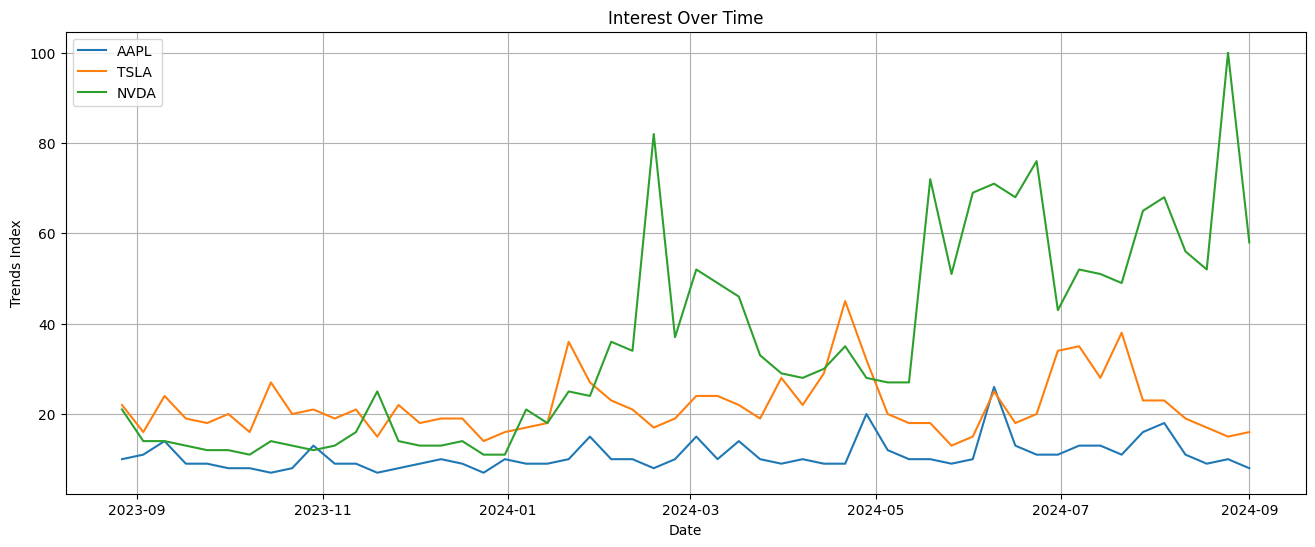
\includegraphics[width=\linewidth,height=0.6\textheight,keepaspectratio]{gfx/m4l2_notes_fig1_google_trends_aapl_tsla_nvda.png}
\par\smallskip{\small \textbf{Hình 1.1:} Mức độ quan tâm theo thời gian (Interest Over Time) trên Google Trends đối với AAPL, TSLA và NVDA, giai đoạn 2023-09-01 đến 2024-09-01}
\end{figure}

Bây giờ khi đã có biểu đồ, dưới đây là một số điểm chính cần chú ý và phân tích:

\textbf{Xu hướng tổng thể:}
\begin{itemize}
  \item Tăng/Giảm: Các xu hướng nhìn chung đang tăng, giảm hay giữ ổn định trong năm? Điều này có thể cho thấy mức độ quan tâm đối với các công ty đang tăng lên hay suy giảm.
  \item Tính mùa vụ: Ta có nhận thấy các mẫu hình hay đỉnh lặp lại vào những thời điểm nhất định trong năm không? Điều này có thể liên quan đến các đợt ra mắt sản phẩm, báo cáo tài chính hoặc các sự kiện khác.
\end{itemize}

\textbf{Mức độ phổ biến tương đối:}
\begin{itemize}
  \item So sánh: Từ khóa nào cho thấy mức độ quan tâm tổng thể cao nhất? Từ khóa nào thấp nhất? Điều này có thể cho ta ý niệm về mức độ phổ biến tương đối của các công ty này xét theo khối lượng tìm kiếm.
  \item Điểm giao nhau: Có những điểm nào mà xu hướng của các từ khóa khác nhau cắt nhau không? Điều này có thể báo hiệu sự thay đổi trong sự chú ý hoặc nhận thức của công chúng.
\end{itemize}

\textbf{Độ biến động:}
\begin{itemize}
  \item Dao động: Các xu hướng dao động nhiều đến mức nào theo thời gian? Những biến động lớn có thể cho thấy sự nhạy cảm với tin tức hoặc các sự kiện thị trường.
  \item Giá trị ngoại lai: Có đỉnh hoặc đáy đáng kể nào nổi bật không? Hãy thử tìm hiểu điều gì có thể đã gây ra chúng (ví dụ: thông báo tin tức, ra mắt sản phẩm, các vụ tranh cãi).
\end{itemize}

\textbf{Tương quan:}
\begin{itemize}
  \item Mối quan hệ: Xu hướng của các từ khóa khác nhau có vẻ di chuyển cùng nhau hay độc lập? Điều này có thể cho biết chúng có chịu ảnh hưởng của các yếu tố tương tự hay không.
\end{itemize}

Bằng cách xem xét cẩn thận các khía cạnh này của biểu đồ, chúng ta có thể có được hiểu biết về hành vi tìm kiếm liên quan đến các công ty này và có khả năng rút ra kết luận về nhận thức của công chúng cũng như hiệu quả hoạt động trên thị trường của họ.

Cụ thể với ví dụ của chúng ta, có thể quan sát thấy các đỉnh và đáy, trong đó NVIDIA (NVDA) có một đỉnh đáng kể vào khoảng tháng 3 năm 2024, gần đạt chỉ số xu hướng (trend index) là 80, và một lần nữa trong giai đoạn gần đây nhất vào cuối tháng 8 năm 2024. Chỉ số cao như vậy có thể trùng với các sự kiện quan trọng liên quan đến NVIDIA, chẳng hạn ra mắt sản phẩm, báo cáo thu nhập hoặc các diễn biến thị trường. Thực tế, vào tháng 3 năm 2024, NVIDIA đã đưa ra những thông báo quan trọng liên quan đến kiến trúc GPU thế hệ tiếp theo có tên Blackwell. Kiến trúc này có 208 tỷ bóng bán dẫn (transistor) đầy ấn tượng và được thiết kế để chạy các mô hình AI tạo sinh theo thời gian thực. Sự kỳ vọng xoay quanh Blackwell nhiều khả năng đã góp phần làm tăng mức độ quan tâm đối với NVIDIA vào thời điểm đó. Ngoài ra, vào tháng 8 năm 2024, NVIDIA tiếp tục công bố các đổi mới liên quan đến AI và hiệu năng trung tâm dữ liệu tại hội nghị Hot Chips, càng thúc đẩy mức độ quan tâm đối với công ty. Những sự kiện và tiến bộ công nghệ này nhiều khả năng giải thích các đỉnh quan tâm được quan sát đối với NVIDIA trong những tháng đó.

Apple (AAPL) và Tesla (TSLA) thể hiện các xu hướng khác nhau trong cùng giai đoạn. Trong khi cả hai công ty nhìn chung duy trì được mức quan tâm, các dao động của họ ít rõ rệt hơn so với NVIDIA. Việc phân tích tin tức hoặc các thông báo của công ty trong những khung thời gian này có thể làm sáng tỏ nguyên nhân đằng sau các xu hướng đó.

Chúng ta cũng cần cân nhắc khám phá tương quan giữa các xu hướng quan tâm đối với các công ty này và các chỉ số thị trường rộng hơn (ví dụ: S\&P 500). Nếu có tương quan dương mạnh, điều đó có thể cho thấy cảm xúc thị trường chung ảnh hưởng đến mức độ quan tâm đối với từng cổ phiếu cụ thể.

Chúng ta cũng cần quan sát bất kỳ mẫu hình lặp lại nào qua các tháng hoặc quý khác nhau. Các yếu tố mùa vụ (ví dụ: mùa lễ, mùa báo cáo thu nhập) có thể tác động đến cảm xúc của nhà đầu tư và mức độ quan tâm.

\begin{itemize}
  \item Các đỉnh của TSLA: Tesla (TSLA) thường có các đỉnh đáng chú ý vào khoảng tháng 4 và tháng 7 mỗi năm. Những đỉnh này có thể trùng với các báo cáo thu nhập hàng quý hoặc các thông báo quan trọng liên quan đến sản phẩm hoặc diễn biến kinh doanh của Tesla.
  \item Xu hướng của AAPL: Apple (AAPL) thường cho thấy xu hướng tăng đều vào khoảng tháng 9 và tháng 1. Những tháng này thường trùng với các đợt ra mắt sản phẩm mới (ví dụ: các đợt phát hành iPhone) và mùa lễ.
  \item Các dao động của NVDA: NVIDIA (NVDA) thể hiện các mẫu hình khó dự đoán hơn, nhưng có các dao động vào khoảng tháng 3 và tháng 8. Hãy tìm hiểu xem có các sự kiện hoặc hội nghị đặc thù của ngành diễn ra trong những tháng này hay không.
\end{itemize}

\subsection*{1.3 Phân tích Mức độ Quan tâm theo các Thước đo khác}

Google Trends cũng cho phép lấy các chi tiết khác liên quan đến truy vấn tìm kiếm của chúng ta:

\begin{itemize}
  \item \textbf{Mức độ quan tâm theo tiểu vùng (Interest by subregion)} cho phép ta xem mức độ quan tâm đối với một từ khóa tìm kiếm cụ thể biến thiên như thế nào giữa các khu vực địa lý khác nhau trong một vùng lớn hơn.
  \item \textbf{Các chủ đề liên quan (Related topics)} là những chủ đề hoặc khái niệm rộng hơn gắn với từ khóa của chúng ta, và cũng được những người dùng khác tìm kiếm.
  \item \textbf{Các truy vấn liên quan (Related queries)} là những từ khóa tìm kiếm cụ thể mà người ta đã dùng kết hợp với từ khóa của chúng ta. Đây là các truy vấn thực tế do những người dùng khác nhập vào công cụ tìm kiếm trong cùng khoảng thời gian.
\end{itemize}

\subsubsection*{Phân tích Mức độ Quan tâm theo Khu vực}

Bây giờ, hãy lấy mức độ quan tâm theo khu vực đối với từ khóa tìm kiếm NVDA và xác định 10 khu vực có mức độ quan tâm cao nhất:

\begin{lstlisting}[language=Python,escapeinside={(*@}{@*)}]
# (*@Khởi@*) (*@tạo@*) (*@một@*) (*@đối@*) (*@tượng@*) (*@của@*) (*@lớp@*) (*@TrendReq@*) (*@và@*) (*@xây@*) (*@dựng@*) (*@payload@*)
pytrends = TrendReq(hl='en-US', tz=360)
pytrends.build_payload(["NVDA"], timeframe='2023-09-01 2024-09-01')

# (*@Lấy@*) (*@dữ@*) (*@liệu@*) (*@mức@*) (*@độ@*) (*@quan@*) (*@tâm@*) (*@theo@*) (*@khu@*) (*@vực@*)
interest_by_region_df = pytrends.interest_by_region()
interest_by_region_df.sort_values(by='NVDA', ascending=False).head(10)
\end{lstlisting}

\begin{lstlisting}[escapeinside={(*@}{@*)}]
               NVDA
geoName
Hong Kong       100
Israel           81
Taiwan           81
United States    65
Singapore        61
Canada           57
China            33
Switzerland      16
South Korea      13
New Zealand      11
\end{lstlisting}

Kết quả này cho thấy 10 khu vực có mức độ quan tâm tìm kiếm cao nhất đối với ``NVDA'' trong giai đoạn đã chỉ định ('2023-09-01 2024-09-01'). Các giá trị biểu thị mức độ phổ biến tương đối của từ khóa tìm kiếm tại mỗi khu vực, trong đó 100 là giá trị cao nhất.

Ví dụ, Hong Kong có mức độ quan tâm tìm kiếm cao nhất đối với ``NVDA'' với giá trị 100, tiếp theo là Đài Loan và Israel với giá trị 79 mỗi nơi. [chưa rõ trong nguyên bản: kết quả chạy hiển thị Israel và Taiwan cùng bằng 81, không phải 79]

Dữ liệu này có thể hữu ích cho các doanh nghiệp để hiểu sự phân bố địa lý của mức độ quan tâm đối với sản phẩm hoặc dịch vụ của họ. Nó cũng có thể được dùng cho nghiên cứu thị trường và để nhận diện các thị trường mục tiêu tiềm năng. Xin lưu ý rằng cần phân tích thêm và đối chiếu với các nguồn dữ liệu khác để rút ra kết luận chắc chắn.

\subsubsection*{Các Truy vấn và Chủ đề Liên quan}

Các chủ đề và truy vấn liên quan hàng đầu (top) và đang tăng (rising) có thể cực kỳ hữu ích cho các tác vụ kỹ thuật tài chính vì chúng cung cấp hiểu biết về ``tâm trí tập thể của thị trường'' và bộc lộ các xu hướng có thể không hiển nhiên từ dữ liệu tài chính truyền thống.

\textbf{Các Chủ đề Liên quan (Related Topics)} là những chủ đề rộng hơn gắn với NVDA. Điều này có thể giúp nhận diện:
\begin{itemize}
  \item Xu hướng ngành: Có các xu hướng rộng hơn trong lĩnh vực game, AI hoặc trung tâm dữ liệu đang ảnh hưởng đến mức độ quan tâm đối với NVDA không?
  \item Chủ đề đầu tư: Có các chủ đề đầu tư cụ thể (ví dụ: cổ phiếu tăng trưởng, cổ phiếu công nghệ) đang thúc đẩy mức độ quan tâm đối với NVDA không?
\end{itemize}

\textbf{Các Truy vấn Liên quan (Related Queries)} là những cụm từ khác mà người ta tìm kiếm kết hợp với từ khóa NVDA. Điều này có thể cho thấy:
\begin{itemize}
  \item Xu hướng mới nổi: Có các từ khóa mới hoặc đang tăng cho thấy sự thay đổi trong mức độ quan tâm hoặc các lĩnh vực trọng tâm mới của NVDA không?
  \item Phân tích đối thủ cạnh tranh: Người ta có tìm kiếm NVDA trong sự so sánh với các đối thủ cạnh tranh của nó không?
  \item Nhận thức của công chúng: Những mối quan ngại hoặc mối quan tâm chính của mọi người về NVDA là gì?
\end{itemize}

Cả Các Chủ đề Liên quan và Các Truy vấn Liên quan đều có thể được lọc để lấy các thuật ngữ Hàng đầu (Top) và Đang tăng (Rising) cho mỗi loại:

\begin{itemize}
  \item \textbf{Top} - đây là các chủ đề/truy vấn tìm kiếm phổ biến nhất. Việc chấm điểm theo thang tương đối, trong đó 100 là chủ đề/truy vấn được tìm kiếm phổ biến nhất, 50 là truy vấn được tìm kiếm với tần suất bằng một nửa, và tiếp tục như vậy.
  \item \textbf{Rising} - đây là các chủ đề/truy vấn có mức tăng tần suất tìm kiếm lớn nhất kể từ giai đoạn trước. Các kết quả được đánh dấu ``Breakout'' có mức tăng rất lớn, có lẽ vì các chủ đề/truy vấn này là mới và có rất ít (nếu có) lượt tìm kiếm trước đó.
\end{itemize}

Trong bài học này, chúng ta sẽ tập trung vào Các Truy vấn Liên quan. Cả các truy vấn liên quan hàng đầu và đang tăng đều mang lại những hiểu biết giá trị, nhưng chúng phục vụ các mục đích khác nhau. Lựa chọn tốt nhất phụ thuộc vào các mục tiêu cụ thể và loại phân tích mà chúng ta đang thực hiện. Từ góc độ kỹ thuật tài chính, việc chọn giữa các truy vấn liên quan hàng đầu và đang tăng vẫn phụ thuộc vào mục tiêu cụ thể của chúng ta, nhưng dưới đây là một khuyến nghị được điều chỉnh sát hơn:

\begin{itemize}
  \item \textbf{Đối với Giao dịch Thuật toán và Phân tích Cảm xúc:} Các truy vấn đang tăng (rising) nhìn chung có giá trị hơn. Chúng có thể cung cấp các tín hiệu thời gian thực cho các chiến lược giao dịch dựa trên cảm xúc. Chúng ta có thể xây dựng một hệ thống tự động điều chỉnh các vị thế danh mục hoặc tạo tín hiệu giao dịch dựa trên những thay đổi trong cảm xúc được thể hiện qua các truy vấn đang tăng. Ví dụ, nếu ta quan sát thấy cảm xúc tiêu cực tăng vọt đột ngột liên quan đến một công ty mà ta đang nắm giữ trong danh mục, thuật toán có thể tự động giảm mức độ phơi nhiễm đối với cổ phiếu đó.

  \item \textbf{Đối với Quản trị Rủi ro:} Các truy vấn đang tăng có vai trò then chốt đối với các dấu hiệu cảnh báo sớm. Một đợt tăng vọt các lượt tìm kiếm cho các từ khóa liên quan đến kiện tụng, điều tra của cơ quan quản lý hoặc thu hồi sản phẩm có thể cho thấy các rủi ro tiềm ẩn đối với một công ty hoặc ngành. Chúng ta có thể tích hợp việc phân tích các truy vấn đang tăng vào hệ thống quản trị rủi ro để chủ động nhận diện và đánh giá các mối đe dọa tiềm ẩn.

  \item \textbf{Đối với Tối ưu hóa Danh mục và Phân bổ Tài sản:} Cả truy vấn hàng đầu và đang tăng đều có thể hữu ích.
  \begin{itemize}
    \item Truy vấn hàng đầu (Top): Có thể giúp hiểu các chủ đề và động lực chính của các tài sản hoặc ngành khác nhau, từ đó cho phép đa dạng hóa danh mục tương ứng.
    \item Truy vấn đang tăng (Rising): Có thể giúp nhận diện các chủ đề mới nổi hoặc các rủi ro tiềm ẩn có thể đòi hỏi điều chỉnh danh mục.
  \end{itemize}

  \item \textbf{Đối với Nghiên cứu Định lượng và Xây dựng Mô hình:} Cả hai loại truy vấn đều có thể có giá trị như các nguồn dữ liệu thay thế.
  \begin{itemize}
    \item Truy vấn đang tăng (Rising): Có thể được dùng để tạo các chỉ báo cảm xúc hoặc tín hiệu phát hiện sự kiện để đưa vào các mô hình định lượng.
    \item Truy vấn hàng đầu (Top): Có thể được dùng để hiểu mối quan hệ giữa các tài sản hoặc ngành khác nhau dựa trên các chủ đề và mối quan ngại được thể hiện trong các truy vấn tìm kiếm.
  \end{itemize}
\end{itemize}

Nhìn chung, trong khi cả hai đều có công dụng riêng, các truy vấn đang tăng có xu hướng có giá trị hơn đối với các ứng dụng kỹ thuật tài chính đòi hỏi hiểu biết theo thời gian thực và tập trung vào các xu hướng ngắn hạn cùng các thay đổi cảm xúc. Các truy vấn hàng đầu mang lại hiểu biết rộng hơn về nhận thức của thị trường, vốn có thể hữu ích cho các chiến lược dài hạn hơn và phân tích cơ bản. Hãy nhớ cân nhắc các thách thức về nhiễu, chất lượng dữ liệu, và nhu cầu về các kỹ thuật phân tích tinh vi khi làm việc với cả hai loại truy vấn.

Cũng xin lưu ý rằng việc thu hẹp khoảng thời gian khi lấy các hiểu biết từ các truy vấn liên quan đang tăng có thể rất có lợi, đặc biệt khi mục tiêu của chúng ta là phát hiện các xu hướng ngắn hạn hoặc nắm bắt các phản ứng tức thời của thị trường. Khung thời gian ngắn hơn nhìn chung mang lại sự cân bằng tốt giữa độ nhạy, khả năng có sẵn của dữ liệu và tính khả thi để hành động. Chúng ta có thể thử nghiệm với các khung thời gian khác nhau để tìm ra khung phù hợp nhất với nhu cầu cụ thể và độ biến động của các tài sản mà ta đang phân tích.

Trong Python, chúng ta có thể lấy các truy vấn liên quan hàng đầu và đang tăng cho một từ khóa tìm kiếm và phân tích kết quả:

\begin{lstlisting}[language=Python,escapeinside={(*@}{@*)}]
# (*@Khởi@*) (*@tạo@*) (*@một@*) (*@đối@*) (*@tượng@*) (*@của@*) (*@lớp@*) (*@TrendReq@*) (*@và@*) (*@xây@*) (*@dựng@*) (*@payload@*)
pytrends = TrendReq(hl='en-US', tz=360)
pytrends.build_payload(["NVDA"], timeframe='2024-08-18 2024-09-01')

# (*@Chờ@*) (*@10@*) (*@giây@*) (*@trước@*) (*@khi@*) (*@gửi@*) (*@yêu@*) (*@cầu@*) (*@tiếp@*) (*@theo@*) (*@để@*) (*@tránh@*) (*@làm@*) (*@quá@*) (*@tải@*) (*@máy@*) (*@chủ@*)
time.sleep(10)

# (*@Lấy@*) (*@các@*) (*@truy@*) (*@vấn@*) (*@liên@*) (*@quan@*)
related_queries_dict = pytrends.related_queries()

# (*@In@*) (*@các@*) (*@truy@*) (*@vấn@*) (*@liên@*) (*@quan@*) (*@hàng@*) (*@đầu@*)
print("Top related queries:")
print(related_queries_dict["NVDA"]["top"])

# (*@In@*) (*@các@*) (*@truy@*) (*@vấn@*) (*@liên@*) (*@quan@*) (*@đang@*) (*@tăng@*)
print("\nRising related queries:")
print(related_queries_dict["NVDA"]["rising"])
\end{lstlisting}

Các truy vấn đang tăng đối với ``NVDA'' cung cấp một số hiểu biết thú vị, đặc biệt liên quan đến thông báo thu nhập sắp tới. Chúng ta có thể rút ra những điều sau:

\begin{itemize}
  \item Thu nhập chiếm ưu thế: Trọng tâm áp đảo là thu nhập của NVDA. Các thuật ngữ liên quan đến thu nhập đều đang tăng mạnh mức độ quan tâm tìm kiếm. Điều này cho thấy mức độ kỳ vọng và quan tâm cao đối với kết quả tài chính của công ty.

  \item Thông tin thời gian thực: Xu hướng ``Breakout'' của ``nvda earnings time today'' cho thấy mọi người đang tích cực tìm kiếm thông tin thời gian thực về thông báo thu nhập, có thể vào ngày công bố.

  \item Mức độ quan tâm toàn cầu: Sự xuất hiện của các ký tự tiếng Nhật và tiếng Trung cho thấy mức độ quan tâm đối với thu nhập của NVDA vượt ra ngoài các khu vực nói tiếng Anh, làm nổi bật tầm với toàn cầu của công ty.

  \item Trọng tâm của nhà đầu tư: Các thuật ngữ như ``nvda investor relations'' và ``when does nvda report earnings'' cho thấy các nhà đầu tư đang tích cực tìm kiếm thông tin về việc công bố thu nhập và có thể đang chuẩn bị cho các phản ứng thị trường tiềm năng.

  \item Tài chính và Nasdaq: Sự gia tăng của ``nasdaq nvda financials'' cho thấy mọi người đang tìm kiếm thông tin tài chính chi tiết về NVDA, có thể trên trang web Nasdaq hoặc các nền tảng tài chính khác.

  \item Các cổ phiếu khác và nhiễu tiềm ẩn: Trong khi các thuật ngữ liên quan đến thu nhập chiếm ưu thế, có một số giá trị ngoại lai như ``lunr stock'', ``pdd stock'', ``crm stock'', ``chwy stock'' và ``afrm stock''. Chúng có thể liên quan đến các công ty hoặc xu hướng thị trường khác và có khả năng là nhiễu trong bối cảnh phân tích NVDA. Cần điều tra thêm để hiểu mức độ liên quan của chúng.
\end{itemize}

\subsection*{1.4 Các Lưu ý và Hạn chế khi sử dụng dữ liệu Google Trends}

Khi sử dụng dữ liệu Google Trends cho phân tích tài chính, chúng ta cần nhận thức được các hạn chế của nó. Dù dữ liệu Google Trends có thể mang lại nhiều hiểu biết, điều quan trọng là phải hiểu các hạn chế của nó về chất lượng dữ liệu. Dưới đây là một số khía cạnh chính cần ghi nhớ:

\begin{itemize}
  \item \textbf{Lấy mẫu:} Dữ liệu Google Trends dựa trên một mẫu các lượt tìm kiếm, không phải toàn bộ khối lượng tìm kiếm, và phương pháp lấy mẫu chính xác không được công bố công khai. Điều này có nghĩa là tồn tại sai số lấy mẫu vốn có, và dữ liệu có thể không đại diện hoàn hảo cho toàn bộ tổng thể các lượt tìm kiếm. Điều này cũng có nghĩa là có thể có một số nhiễu và dữ liệu có thể không phản ánh hoàn hảo mức độ quan tâm tìm kiếm thực tế.
  \item \textbf{Cập nhật dữ liệu:} Dữ liệu Google Trends có thể được cập nhật hoặc điều chỉnh theo thời gian khi Google cải tiến các thuật toán và kỹ thuật xử lý dữ liệu của mình. Điều này có nghĩa là dữ liệu lịch sử mà bạn đã truy cập trước đây có thể thay đổi đôi chút trong tương lai.
  \item \textbf{Chuẩn hóa:} Dữ liệu Google Trends được chuẩn hóa, nghĩa là các giá trị mang tính tương đối so với điểm cao nhất trong khung thời gian bạn chọn. Dữ liệu được chuẩn hóa về thang từ 0 đến 100. Giá trị 100 biểu thị mức phổ biến đỉnh điểm, trong khi các giá trị khác được co giãn theo tỷ lệ. Điều này có nghĩa là các giá trị biểu thị mức độ phổ biến tương đối của một từ khóa tìm kiếm so với điểm cao nhất trong khung thời gian được chọn. Trong khi việc chuẩn hóa giúp so sánh các xu hướng, nó cũng có thể che khuất khối lượng tìm kiếm tuyệt đối, vốn có thể liên quan trong một số trường hợp.
  \item \textbf{Độ chi tiết địa lý:} Mức độ chi tiết về địa lý của dữ liệu Google Trends thay đổi tùy theo từ khóa tìm kiếm và khoảng thời gian. Với một số từ khóa hoặc khu vực, dữ liệu có thể chi tiết hơn, trong khi với những nơi khác, dữ liệu có thể mang tính tổng hợp hơn. Điều này có thể ảnh hưởng đến độ chính xác của phân tích theo khu vực.
  \item \textbf{Các yếu tố bên ngoài:} Hành vi tìm kiếm có thể chịu ảnh hưởng của nhiều yếu tố bên ngoài, như mức độ đưa tin của truyền thông, các sự kiện tin tức, tính mùa vụ, và thậm chí mức độ phổ biến của các từ khóa tìm kiếm khác. Những yếu tố này có thể đưa nhiễu và thiên lệch vào dữ liệu, gây khó khăn cho việc tách biệt các xu hướng nền tảng thực sự.
  \item \textbf{Quyền riêng tư:} Dữ liệu Google Trends đã được ẩn danh hóa và tổng hợp, nhưng vẫn cần lưu ý đến các cân nhắc về quyền riêng tư, đặc biệt khi xử lý các chủ đề nhạy cảm.
\end{itemize}

Bằng cách hiểu các cân nhắc về chất lượng dữ liệu này và thực hiện các biện pháp phòng ngừa phù hợp, chúng ta có thể sử dụng dữ liệu Google Trends hiệu quả hơn và rút ra các kết luận đáng tin cậy hơn cho phân tích tài chính. Hãy nhớ rằng bối cảnh là chìa khóa. Chúng ta cần xem xét bối cảnh xung quanh dữ liệu, chẳng hạn các yếu tố bên ngoài tiềm năng có thể đang ảnh hưởng đến hành vi tìm kiếm.

\section*{2. Phân tích Ngữ nghĩa Tiềm ẩn (Latent Semantic Analysis)}

Cho đến nay chúng ta đã khám phá dữ liệu Google Trends và các ví dụ đơn giản về việc dùng \texttt{pytrends} để thu thập dữ liệu. Trong khi bản thân \texttt{pytrends} cung cấp những hiểu biết giá trị về các xu hướng tìm kiếm, việc đưa vào các kỹ thuật học máy như Phân tích Ngữ nghĩa Tiềm ẩn (LSA) có thể mang lại nhiều lợi thế.

Trước khi giới thiệu LSA, chúng ta cần hiểu một số thuật ngữ. Trong ngữ cảnh của LSA, một ``\textbf{tài liệu}'' (document) là một đơn vị văn bản mà chúng ta muốn phân tích. Nó có thể là bất cứ thứ gì từ một câu đơn lẻ đến cả một bài báo, một cuốn sách, hoặc thậm chí một tập hợp các văn bản liên quan. Điều then chốt là nó đại diện cho một phần thông tin riêng biệt mà chúng ta muốn so sánh và phân tích trong mối quan hệ với các tài liệu khác. Dưới đây là một số ví dụ về những gì có thể được coi là một ``tài liệu'' trong các ứng dụng LSA khác nhau:

\begin{itemize}
  \item \textbf{Mô hình hóa chủ đề (Topic Modeling):} Mỗi tài liệu có thể là một bài báo, một bài blog, hoặc một bài đăng trên mạng xã hội. LSA có thể giúp nhận diện các chủ đề chính được thảo luận trong các tài liệu này.
  \item \textbf{Truy xuất thông tin (Information Retrieval):} Mỗi tài liệu có thể là một trang web, một bài nghiên cứu, hoặc một mô tả sản phẩm. LSA có thể giúp tìm các tài liệu tương tự về mặt ngữ nghĩa với một truy vấn cho trước.
  \item \textbf{Phân loại tài liệu (Document Classification):} Mỗi tài liệu có thể là một email, một đánh giá của khách hàng, hoặc một hợp đồng pháp lý. LSA có thể giúp phân loại các tài liệu này dựa trên nội dung của chúng.
\end{itemize}

Phân tích Ngữ nghĩa Tiềm ẩn (LSA) là một kỹ thuật trong xử lý ngôn ngữ tự nhiên, phân tích mối quan hệ giữa một tập hợp các tài liệu và các thuật ngữ mà chúng chứa bằng cách tạo ra một tập hợp các khái niệm liên quan đến các tài liệu và thuật ngữ. LSA giả định rằng những từ có nghĩa gần nhau sẽ xuất hiện trong các đoạn văn bản tương tự. Việc đưa vào các kỹ thuật học máy như LSA có thể mang lại nhiều lợi thế:

\begin{itemize}
  \item \textbf{Khám phá các mối quan hệ ẩn:} LSA có thể bộc lộ các mối quan hệ ẩn giữa các thuật ngữ và khái niệm mà có thể không hiển nhiên khi chỉ nhìn vào dữ liệu tìm kiếm thô. Điều này có thể giúp ta hiểu cấu trúc ngữ nghĩa nền tảng của các truy vấn tìm kiếm liên quan đến các tài liệu của chúng ta.

  \item \textbf{Giảm chiều dữ liệu:} LSA có thể giảm số chiều của dữ liệu bằng cách biểu diễn nó trong một không gian khái niệm có số chiều thấp hơn. Điều này có thể giúp phân tích và trực quan hóa dữ liệu dễ dàng hơn, đặc biệt khi xử lý số lượng lớn thuật ngữ.

  \item \textbf{Cải thiện tìm kiếm và gợi ý:} Bằng cách hiểu mối quan hệ giữa các thuật ngữ và khái niệm, chúng ta có thể xây dựng các công cụ tìm kiếm và hệ thống gợi ý thông minh hơn. Ví dụ, ta có thể gợi ý các tìm kiếm liên quan hoặc đề xuất tài liệu dựa trên độ tương đồng ngữ nghĩa thay vì chỉ khớp từ khóa.

  \item \textbf{Mô hình hóa chủ đề:} LSA có thể được dùng cho mô hình hóa chủ đề, cho phép ta khám phá các chủ đề hoặc đề tài chính hiện diện trong một tập hợp tài liệu hoặc truy vấn tìm kiếm. Điều này có thể giúp ta hiểu bối cảnh rộng hơn của thông tin và có khả năng phân loại hoặc phân cụm tài liệu hiệu quả hơn.
\end{itemize}

Nói ngắn gọn, LSA được dùng để phân tích dữ liệu văn bản và là một phương pháp trích xuất và biểu diễn ý nghĩa theo cách dùng trong ngữ cảnh của các từ, thông qua các tính toán thống kê áp dụng trên một kho ngữ liệu văn bản lớn. LSA là một công cụ mạnh để phân tích dữ liệu văn bản, nhưng có một số hạn chế. Ví dụ, nó không xử lý tốt hiện tượng đa nghĩa (polysemy, các từ có nhiều nghĩa) hay đồng nghĩa (synonymy, các từ khác nhau có cùng nghĩa).

Trong bài học này, chúng ta sẽ khám phá một ví dụ cơ bản về cách có thể dùng LSA để phân tích các từ khóa tìm kiếm liên quan và cải thiện hiểu biết của chúng ta về hành vi tìm kiếm của người dùng. Việc coi cái gì là một tài liệu phụ thuộc vào ứng dụng cụ thể và loại phân tích mà ta muốn thực hiện. Điều quan trọng là đảm bảo các tài liệu của chúng ta có ý nghĩa và phù hợp với tác vụ đang thực hiện. Một tập hợp các tài liệu được gọi chung là ``\textbf{ma trận thuật ngữ-tài liệu}'' (term-document matrix).

Các kỹ sư tài chính có thể tiếp cận việc hình thành tài liệu cho LSA hoặc các kỹ thuật tương tự theo những cách khác nhau:

\begin{itemize}
  \item Chuyên môn lĩnh vực: Các kỹ sư tài chính thường có chuyên môn sâu về lĩnh vực và cẩn thận chọn các từ khóa và cụm từ dựa trên hiểu biết của họ về thị trường tài chính, các tài sản cụ thể và các sự kiện liên quan.

  \item Nguồn dữ liệu: Họ có thể sử dụng phạm vi nguồn dữ liệu rộng hơn so với chỉ Google Trends, chẳng hạn các bài báo tin tức và phân tích cảm xúc, dữ liệu mạng xã hội, hồ sơ công ty và bản ghi các cuộc họp báo cáo thu nhập, các tập dữ liệu độc quyền.

  \item Tiền xử lý tinh vi: Họ có thể sử dụng các kỹ thuật xử lý ngôn ngữ tự nhiên nâng cao hơn cho bước tiền xử lý, bao gồm nhận dạng thực thể có tên (nhận diện các công ty, con người, địa điểm), phân tích cảm xúc (gán điểm cảm xúc cho văn bản), mô hình hóa chủ đề (nhận diện các chủ đề nền tảng trong tài liệu).

  \item Các phương pháp tổ hợp (Ensemble Methods): Họ có thể kết hợp LSA với các kỹ thuật học máy khác hoặc dùng các phương pháp tổ hợp để cải thiện độ chính xác và tính vững của mô hình.

  \item Kiểm định lùi và xác thực (Backtesting and Validation): Các kỹ sư tài chính kiểm định lùi và xác thực các mô hình của họ một cách nghiêm ngặt bằng dữ liệu lịch sử để đảm bảo chúng đáng tin cậy và có khả năng tạo ra các tín hiệu giao dịch hoặc chiến lược đầu tư sinh lời.
\end{itemize}

Với ví dụ của chúng ta, chúng ta sẽ tạo ma trận thuật ngữ-tài liệu với tập hợp các tài liệu sau:

\begin{quote}
Document 1: ``Risk management in derivatives trading'', \\
Document 2: ``Portfolio optimization techniques and strategies'', \\
Document 3: ``Algorithmic trading and its impact on market efficiency'', \\
Document 4: ``Quantitative methods for financial modeling'', \\
Document 5: ``High-frequency trading and liquidity provision'', \\
Document 6: ``Integrating Derivatives into Portfolio Optimization Strategies'', \\
Document 7: ``High-Frequency Trading Strategies: Algorithmic Approaches and Market Impact'', \\
Document 8: ``Quantitative Methods for Algorithmic Trading and Portfolio Optimization''
\end{quote}

Trước khi tiếp tục với mã, hãy lưu ý rằng các tài liệu trong ma trận thuật ngữ-tài liệu của chúng ta chứa những từ như ``in'', ``and'', ``for'', ``on''. Những từ này được gọi là \textbf{từ dừng} (stop words). Chúng là các từ thông dụng, nhìn chung không mang nhiều ý nghĩa cụ thể trong ngữ cảnh phân tích văn bản. Thường có lợi khi loại bỏ từ dừng khỏi dữ liệu văn bản trước khi tạo ma trận thuật ngữ-tài liệu. Điều này có thể giúp:

\begin{itemize}
  \item \textbf{Giảm nhiễu:} Từ dừng có thể thêm nhiễu vào dữ liệu và che khuất các thuật ngữ quan trọng hơn vốn truyền tải các chủ đề hoặc đề tài chính.
  \item \textbf{Cải thiện hiệu quả:} Loại bỏ từ dừng có thể giảm kích thước ma trận, giúp việc tính toán nhanh và hiệu quả hơn.
  \item \textbf{Tập trung vào các thuật ngữ liên quan:} Bằng cách loại bỏ các từ thông dụng, chúng ta có thể tập trung vào các thuật ngữ có ý nghĩa hơn, đặc thù cho các tài liệu và ứng dụng của mình.
\end{itemize}

Chúng ta cũng sẽ áp dụng kỹ thuật lemmatization (chuẩn hóa về dạng gốc từ điển). \textbf{Stemming (rút gọn về gốc từ) và lemmatization} là hai kỹ thuật tiền xử lý văn bản được dùng trong Xử lý ngôn ngữ tự nhiên (NLP) giúp rút gọn các từ về dạng cơ sở của chúng.
\begin{itemize}
  \item \textbf{Stemming} rút gọn các từ về thân từ (stem), vốn không nhất thiết là từ có thật, bằng cách loại bỏ tiền tố và hậu tố. Ví dụ ``playing'' sẽ thành ``play'', ``studies'' sẽ thành ``studi'', và ``happily'' sẽ thành ``happi''.
  \item \textbf{Lemmatization} rút gọn các từ về dạng từ điển hoặc dạng cơ sở gọi là lemma. Ví dụ ``playing'' sẽ thành ``play'', ``studies'' sẽ thành ``study'', và ``better'' sẽ thành ``good''.
\end{itemize}

Trong ví dụ của chúng ta, chúng ta sử dụng lemmatization: với ngôn ngữ đặc thù và có thể có nhiều sắc thái của tài chính, lemmatization nhiều khả năng có lợi hơn stemming. Nó có thể giúp nhóm các dạng khác nhau của từ (ví dụ: ``analyze'', ``analyzing'', ``analysis'') trong khi vẫn giữ được ý nghĩa cốt lõi của chúng.

Bây giờ khi đã làm rõ mọi thuật ngữ cơ bản và định nghĩa LSA, hãy tiến hành chuẩn bị dữ liệu. Đoạn mã Python sau thực hiện đúng việc đó:

\begin{lstlisting}[language=Python,escapeinside={(*@}{@*)}]
# (*@Các@*) (*@tài@*) (*@liệu@*) (*@mẫu@*)
documents = [
    "Risk management in derivatives trading",
    "Portfolio optimization techniques and strategies",
    "Algorithmic trading and its impact on market efficiency",
    "Quantitative methods for financial modeling",
    "High-frequency trading and liquidity provision",
    "Integrating Derivatives into Portfolio Optimization Strategies",
    "High-Frequency Trading Strategies: Algorithmic Approaches and Market Impact",
    "Quantitative Methods for Algorithmic Trading and Portfolio Optimization"
]

# (*@Tải@*) (*@stopwords@*) (*@và@*) (*@tài@*) (*@nguyên@*) (*@WordNet@*) (*@rồi@*) (*@tạo@*) (*@một@*) (*@đối@*) (*@tượng@*) (*@Lemmatizer@*)
nltk.download('stopwords')
nltk.download('wordnet')
nltk.download('punkt')
lemmatizer = WordNetLemmatizer()

# (*@Xây@*) (*@dựng@*) (*@hàm@*) (*@tiền@*) (*@xử@*) (*@lý@*) (*@văn@*) (*@bản@*)
def preprocess_text(text):
    text = re.sub(r'[^\w\s-]', '', text)  # (*@Loại@*) (*@bỏ@*) (*@dấu@*) (*@câu@*) (*@ngoại@*) (*@trừ@*) (*@dấu@*) (*@gạch@*) (*@nối@*)
    tokens = nltk.word_tokenize(text.lower())
    tokens = [lemmatizer.lemmatize(token) for token in tokens] # (*@Lemmatize@*)
    stop_words = set(stopwords.words('english')) # (*@định@*) (*@nghĩa@*) (*@stop\_words@*) (*@là@*) (*@tập@*) (*@hợp@*) (*@các@*) (*@từ@*) (*@dừng@*) (*@tiếng@*) (*@Anh@*)
    tokens = [token for token in tokens if token not in stop_words] # (*@Loại@*) (*@bỏ@*) (*@từ@*) (*@dừng@*)
    return tokens

# (*@Tạo@*) (*@một@*) (*@đối@*) (*@tượng@*) (*@CountVectorizer@*)
vectorizer = CountVectorizer(tokenizer=preprocess_text, token_pattern=None)

# (*@Tạo@*) (*@ma@*) (*@trận@*) (*@thuật@*) (*@ngữ-tài@*) (*@liệu,@*) (*@rồi@*) (*@chuyển@*) (*@thành@*) (*@một@*) (*@DataFrame@*) (*@của@*) (*@pandas@*)
term_document_matrix = vectorizer.fit_transform(documents)
df = pd.DataFrame(term_document_matrix.toarray(), columns = vectorizer.get_feature_names_out())
term_document_matrix = df.T
print(term_document_matrix)
\end{lstlisting}

Ma trận này cho thấy các mối quan hệ giữa các thuật ngữ (hàng) và các tài liệu (cột). Ví dụ:

\begin{itemize}
  \item Thuật ngữ ``algorithmic'' xuất hiện (giá trị 1) trong các tài liệu 3, 7 và 8.
  \item Thuật ngữ ``trading'' xuất hiện trong các tài liệu 1, 3, 5, 7 và 8.
  \item Tài liệu 1 chứa các thuật ngữ ``derivatives'', ``management'', ``risk'' và ``trading''.
\end{itemize}

Ma trận này là nền tảng để áp dụng LSA hoặc các kỹ thuật giảm chiều khác.

\subsection*{2.1 LSA liên hệ với SVD như thế nào}

LSA sử dụng Phân rã Giá trị Kỳ dị (Singular Value Decomposition, SVD) ở cốt lõi để tìm các mối quan hệ ẩn giữa các thuật ngữ và khái niệm. Phân rã Giá trị Kỳ dị là một khái niệm nền tảng trong đại số tuyến tính và là một kỹ thuật mạnh được dùng trong nhiều lĩnh vực, bao gồm học máy và xử lý ngôn ngữ tự nhiên. Cách thức hoạt động như sau:

\begin{enumerate}
  \item Ma trận Tài liệu-Thuật ngữ: LSA bắt đầu với một ma trận tài liệu-thuật ngữ, trong đó mỗi hàng đại diện cho một tài liệu và mỗi cột đại diện cho một thuật ngữ (từ). Các ô chứa tần suất của mỗi thuật ngữ trong mỗi tài liệu.

  \item Áp dụng SVD hay Phân tích Ma trận thành nhân tử: SVD được áp dụng lên ma trận Tài liệu-Thuật ngữ. SVD là một cách phân tích (chia nhỏ) một ma trận thành ba ma trận riêng biệt. Nó phân rã ma trận thành ba ma trận:
  \begin{itemize}
    \item $U$: Biểu diễn độ tương đồng giữa tài liệu và khái niệm.
    \item $\Sigma$: Một ma trận đường chéo chứa các giá trị kỳ dị, biểu diễn tầm quan trọng của mỗi khái niệm.
    \item $V$: Biểu diễn độ tương đồng giữa thuật ngữ và khái niệm.
    \item Công thức: Mối quan hệ giữa ma trận gốc ($A$) và các ma trận phân rã là: $A = U \Sigma V^T$ (trong đó $V^T$ là chuyển vị của $V$).
  \end{itemize}

  \item Giảm chiều: Bằng cách chỉ giữ lại các giá trị kỳ dị lớn nhất (và các cột/hàng tương ứng trong $U$ và $V$), chúng ta giảm số chiều (khái niệm) trong khi vẫn bảo toàn thông tin quan trọng nhất. Điều này tương tự Phân tích Thành phần Chính (PCA).

  \item Không gian Khái niệm: Các ma trận thu được biểu diễn các tài liệu và thuật ngữ trong một ``không gian khái niệm'' mới. Các từ có nghĩa tương tự sẽ nằm gần nhau hơn trong không gian này, ngay cả khi chúng không xuất hiện trong cùng các tài liệu.
\end{enumerate}

Về bản chất, SVD trong LSA giúp:

\begin{itemize}
  \item \textbf{Khám phá các mối quan hệ tiềm ẩn:} Nhận diện các khái niệm nền tảng không hiện diện tường minh trong văn bản.
  \item \textbf{Giảm nhiễu:} Lọc bỏ thông tin ít quan trọng hơn và tập trung vào ý nghĩa cốt lõi.
  \item \textbf{Cải thiện truy xuất thông tin:} Biểu diễn tài liệu và truy vấn theo cách nắm bắt được độ tương đồng ngữ nghĩa.
\end{itemize}

Quá trình này cho phép LSA vượt ra ngoài việc khớp từ khóa đơn giản và hiểu ý nghĩa của văn bản ở mức sâu hơn.

Bây giờ hãy tiếp tục với mã Python, trong đó chúng ta sẽ dùng \texttt{TruncatedSVD} từ \texttt{scikit-learn}, về bản chất là thực hiện Phân rã Giá trị Kỳ dị (SVD) ở bên dưới. \texttt{TruncatedSVD} là một cách triển khai SVD hiệu quả được thiết kế riêng cho việc giảm chiều. Nó tính SVD rồi chỉ giữ lại \texttt{n\_components} giá trị kỳ dị lớn nhất cùng các vector tương ứng của chúng. Phiên bản SVD rút gọn (truncated) này là thứ tạo ra \texttt{lsa\_matrix}, biểu diễn dữ liệu của chúng ta trong một không gian khái niệm có số chiều thấp hơn.

\textbf{Quan trọng:} Kết quả đầu ra của LSA có thể khác nhau mỗi lần chúng ta chạy mã. Điều này là do việc khởi tạo ngẫu nhiên của thuật toán \texttt{TruncatedSVD}. Sự biến thiên liên quan đến bản chất của Phân rã Giá trị Kỳ dị (SVD) và cách LSA sử dụng nó. Dưới đây là phân tích các yếu tố chính:

\begin{itemize}
  \item Phép quay trong Không gian Khái niệm: SVD về bản chất tìm cách tốt nhất để biểu diễn dữ liệu của chúng ta trong một ``không gian khái niệm'' mới. Các thành phần (hay chiều) trong không gian này được xác định bằng cách tìm các hướng có phương sai lớn nhất trong dữ liệu gốc. Tuy nhiên, thường có một mức độ linh hoạt trong cách các thành phần này được định hướng (xoay). Hãy hình dung như việc xoay một vật thể 3D: vật thể vẫn như cũ, nhưng phép chiếu của nó lên các trục thay đổi.

  \item Tính mơ hồ về dấu: Dấu (dương hoặc âm) của các giá trị trong kết quả LSA có thể đảo mà không làm thay đổi ý nghĩa nền tảng. Đó là vì hướng của một thành phần là tùy ý. Hãy tưởng tượng một thành phần biểu diễn ``financial modeling'': việc nó hướng về một phía hay phía ngược lại không quan trọng, nó vẫn nắm bắt cùng một khái niệm.

  \item Độ nhạy với các thay đổi nhỏ: SVD có thể nhạy cảm với các thay đổi nhỏ trong dữ liệu đầu vào. Ngay cả những biến thể nhỏ về tần suất từ hoặc việc thêm/bớt một vài tài liệu cũng có thể dẫn đến một mức độ xoay nào đó trong không gian khái niệm, dẫn đến các trọng số thuật ngữ (term loadings) khác nhau.

  \item Khởi tạo ngẫu nhiên: Như đã đề cập, thuật toán TruncatedSVD thường dùng khởi tạo ngẫu nhiên, điều này có thể góp phần gây ra các biến thể trong kết quả.
\end{itemize}

Trong khi những biến thể này có vẻ đáng lo ngại, chúng thường không làm thay đổi đáng kể cách diễn giải tổng thể các kết quả LSA. Vị trí tương đối của các thuật ngữ trong không gian khái niệm và các mẫu hình tương đồng chung nhìn chung được bảo toàn. Để đảm bảo kết quả nhất quán, chúng ta sẽ đặt tham số \texttt{random\_state} về một giá trị cố định khi tạo đối tượng \texttt{TruncatedSVD}. Điều này sẽ cho ra cùng một kết quả mỗi lần chúng ta chạy mã.

\begin{lstlisting}[language=Python,escapeinside={(*@}{@*)}]
# (*@Lấy@*) (*@các@*) (*@thuật@*) (*@ngữ@*) (*@(từ)@*) (*@từ@*) (*@ma@*) (*@trận@*) (*@thuật@*) (*@ngữ-tài@*) (*@liệu@*)
terms = term_document_matrix.index

# (*@Tạo@*) (*@một@*) (*@mô@*) (*@hình@*) (*@LSA@*) (*@và@*) (*@khớp@*) (*@với@*) (*@term\_document\_matrix@*)
lsa = TruncatedSVD(n_components=2, random_state=42)
lsa_matrix = lsa.fit_transform(term_document_matrix)

# (*@Tạo@*) (*@DataFrame@*) (*@cho@*) (*@kết@*) (*@quả@*) (*@LSA@*) (*@với@*) (*@tên@*) (*@thuật@*) (*@ngữ@*) (*@và@*) (*@in@*) (*@ra@*)
df_lsa = pd.DataFrame(lsa_matrix, index=terms)
print(df_lsa)
\end{lstlisting}

Việc diễn giải các kết quả LSA đòi hỏi hiểu không gian ngữ nghĩa mới được tạo ra bởi việc giảm chiều và phân tích các mối quan hệ giữa thuật ngữ và tài liệu trong không gian này. Dưới đây là cách diễn giải các kết quả:

\begin{itemize}
  \item Diễn giải các cột: Chúng còn được gọi là Thành phần (Components) hay Khái niệm (Concepts) hay Chiều (Dimensions). Hãy coi mỗi thành phần như đại diện cho một ``khái niệm'' hoặc ``chủ đề'' ẩn trong các tài liệu.
  \item Diễn giải các hàng: Mỗi hàng trong ma trận này đại diện cho một thuật ngữ từ ma trận gốc của chúng ta, nhưng nay được chiếu lên một không gian khái niệm 2 chiều (vì chúng ta chọn \texttt{n\_components=2}).
  \item Diễn giải các giá trị:
  \begin{itemize}
    \item Hai giá trị trong mỗi hàng biểu diễn tọa độ của thuật ngữ đó trong không gian khái niệm mới. Các thuật ngữ có tọa độ tương tự nằm gần nhau hơn trong không gian khái niệm, cho thấy mối quan hệ ngữ nghĩa. Trong ví dụ của chúng ta, hàng đầu tiên đại diện cho thuật ngữ ``algorithmic''. Tọa độ của nó xấp xỉ (1.488 -0.458). Nếu một thuật ngữ khác có tọa độ tương tự, điều đó cho thấy các thuật ngữ này có liên quan trong ngữ cảnh các tài liệu của chúng ta.
    \item Các giá trị biểu diễn trọng số (loading) của thuật ngữ đó trên thành phần tương ứng. Các trọng số cho ta biết mỗi thuật ngữ đóng góp bao nhiêu vào khái niệm đó. Ví dụ, ``algorithmic'' và ``trading'' có trọng số cao trên Thành phần 1, cho thấy Thành phần 1 đại diện cho khái niệm ``algorithmic trading''. Giá trị càng cao (dương hoặc âm) cho thấy mối liên hệ giữa thuật ngữ và thành phần đó càng mạnh.
  \end{itemize}
\end{itemize}

Từ kết quả đầu ra của mã, chúng ta có thể diễn giải mối quan hệ giữa các thuật ngữ bằng cách xem xét tọa độ của chúng và rút ra một số quan sát sơ bộ:

\begin{itemize}
  \item \textbf{Các cụm riêng biệt:}
  \begin{itemize}
    \item Cụm Giao dịch (Trading): ``algorithmic'', ``high-frequency'', ``impact'', ``market'' và ``trading'' có giá trị cao ở thành phần 0 và chủ yếu là giá trị âm ở thành phần 1. Điều này củng cố ý tưởng rằng thành phần 0 đại diện cho các khái niệm liên quan đến giao dịch tự động và tần suất cao, cùng tác động tiềm ẩn của chúng lên thị trường.

    \item Cụm Danh mục đầu tư và Tối ưu hóa: ``optimization'' và ``portfolio'' tạo thành một cụm rõ ràng với giá trị dương cao ở cả hai thành phần. Điều này cho thấy mối liên hệ mạnh giữa các thuật ngữ này, có khả năng liên quan đến các kỹ thuật tối ưu hóa danh mục đầu tư.

    \item Cụm Phái sinh và Phương pháp-Định lượng: Việc nhóm ``method'', ``quantitative'' và ``derivative'' lại với nhau cho thấy một mối liên hệ tiềm năng giữa các phương pháp định lượng và ứng dụng của chúng vào các công cụ phái sinh.

    \item Cụm Quản lý-Rủi ro-Thanh khoản-Cung ứng: Việc kết hợp ``management'', ``risk'', ``liquidity'' và ``provision'' cho thấy một cụm liên quan đến việc quản lý rủi ro tài chính và đảm bảo thanh khoản. Điều này cũng có vẻ hợp lý, vì các khái niệm này thường đan xen trong các bối cảnh tài chính, đặc biệt khi xử lý các công cụ phái sinh hoặc hoạt động giao dịch.
  \end{itemize}

  \item \textbf{Các quan sát khác:}
  \begin{itemize}
    \item ``Trading'' như một khái niệm trung tâm: ``trading'' có giá trị cao nhất ở thành phần 0, cho thấy tầm quan trọng của nó và mối liên hệ tiềm năng với nhiều hình thức giao dịch được thảo luận trong các tài liệu.
    \item Cặp riêng biệt: Cặp thuật ngữ ``financial'' và ``modeling'' tạo thành một cặp rất riêng biệt do có tọa độ giống hệt nhau. Cần phân tích thêm để xác định mối quan hệ của chúng với các thuật ngữ và cụm khác.
    \item Sự chồng lấn giữa các cụm: Một số thuật ngữ, như ``strategy'' và ``technique'', có giá trị vừa phải ở nhiều thành phần, cho thấy khả năng chồng lấn hoặc kết nối giữa các cụm khác nhau.
  \end{itemize}
\end{itemize}

Phân tích nhanh này cho một cái nhìn tổng quan khá tốt về mối quan hệ giữa các thuật ngữ dựa trên kết quả LSA.

Bây giờ chúng ta có thể vẽ các tọa độ để trực quan hóa chúng và xác nhận xem các cụm được đề xuất này có xuất hiện gần nhau trong biểu diễn trực quan hay không. Để thực hiện điều này, chúng ta sẽ dùng mô-đun \texttt{plotly.graph\_objects} được nhập với tên \texttt{go}:

\begin{lstlisting}[language=Python,escapeinside={(*@}{@*)}]
# (*@Tạo@*) (*@danh@*) (*@sách@*) (*@các@*) (*@văn@*) (*@bản@*) (*@hiển@*) (*@thị@*) (*@khi@*) (*@rê@*) (*@chuột@*) (*@(hover)@*) (*@với@*) (*@nhãn@*) (*@và@*) (*@tọa@*) (*@độ@*)
hover_texts = []
for row in df_lsa.values:
    terms = df_lsa.index[(df_lsa[0] == row[0]) & (df_lsa[1] == row[1])]
    terms_str = ', '.join([f'"{term}"' for term in terms])
    coord = f"({row[0]:.5f}, {row[1]:.5f})"
    hover_texts.append(f"Terms: {terms_str}<br>{coord}")

# (*@Tạo@*) (*@biểu@*) (*@đồ@*) (*@phân@*) (*@tán@*)
fig = go.Figure(go.Scatter(
    x=df_lsa[0],
    y=df_lsa[1],
    mode='markers',
    marker=go.scatter.Marker(
        size=10,
        color='blue',
        opacity=0.8
    ),
    hovertemplate='%{text}<extra></extra>',
    text=hover_texts
))

# (*@Đặt@*) (*@nhãn@*) (*@trục@*) (*@và@*) (*@tiêu@*) (*@đề@*)
fig.update_layout(
    xaxis_title="Component 0",
    yaxis_title="Component 1",
    title="LSA Results Scatter Plot"
)

fig.show()
\end{lstlisting}

Các biểu đồ Plotly có tính tương tác theo mặc định. Chúng ta có thể dùng các tính năng tương tác của nó để kéo/thu phóng và rê chuột/chọn để xem chú giải công cụ (tooltip) với nhãn thuật ngữ và tọa độ.

Bây giờ nhìn vào biểu đồ này, có vẻ như các cụm không dễ trực quan hóa lắm. Có vẻ chúng ta đã quá tập trung vào các giá trị vừa phải của tọa độ thuật ngữ, mà không chú ý đủ đến khoảng cách chính xác giữa chúng. Để xác định các cụm chính xác hơn, chúng ta nên dùng các phương pháp hình thức hơn. Bằng cách sử dụng các phương pháp này, chúng ta có thể tránh các diễn giải chủ quan và xác định các cụm chính xác hơn dựa trên các thước đo định lượng về độ tương đồng hoặc khoảng cách. Chúng ta sẽ xem xét các phương pháp này ở phần sau của bài học.

\subsection*{2.2 Những Cân nhắc Quan trọng với LSA và SVD}

\subsubsection*{Chọn số thành phần tối ưu cho LSA}

Việc chọn số thành phần tối ưu (\texttt{n\_components}) cho LSA là một bước then chốt. Dưới đây là một số cân nhắc:

\begin{itemize}
  \item \textbf{Bắt đầu nhỏ:} Bắt đầu với số lượng thành phần nhỏ (ví dụ: 2, 3 hoặc 5) để xem liệu nó có cho hiểu biết ban đầu tốt về mối quan hệ giữa thuật ngữ và tài liệu hay không. Điều này có thể giúp nắm bắt cảm nhận về dữ liệu và nhận diện các cụm hoặc chủ đề tiềm năng.
  \item \textbf{Tăng dần lặp lại:} Tăng dần số lượng thành phần và quan sát cách diễn giải các kết quả thay đổi. Hãy tìm điểm mà việc thêm thành phần không còn cải thiện đáng kể khả năng diễn giải hoặc không bộc lộ thêm các mối quan hệ có ý nghĩa mới.
  \item \textbf{Cân nhắc kích thước kho ngữ liệu:} Với các kho ngữ liệu nhỏ hơn, ít thành phần hơn có thể là đủ để tránh quá khớp (overfitting). Với các kho ngữ liệu lớn hơn, nhiều thành phần hơn có thể nắm bắt các mối quan hệ ngữ nghĩa tinh tế hơn.
  \item \textbf{Tập trung vào sự mạch lạc ngữ nghĩa:} Đánh giá sự mạch lạc ngữ nghĩa của các chủ đề hoặc cụm thu được. Các thuật ngữ trong mỗi cụm có hợp lý khi đi cùng nhau không? Các cụm có riêng biệt và có ý nghĩa không? Nếu độ mạch lạc giảm khi ta thêm thành phần, đó có thể là dấu hiệu cho thấy ta bắt đầu quá khớp.
  \item \textbf{Cân bằng giữa giảm chiều và mất thông tin:} LSA liên quan đến sự đánh đổi giữa giảm số chiều và bảo toàn thông tin. Chúng ta nên tìm điểm cân bằng tối ưu, nơi ta có số lượng thành phần có thể quản lý được trong khi vẫn nắm bắt các mối quan hệ ngữ nghĩa quan trọng nhất.
\end{itemize}

Tóm lại, không có câu trả lời chung cho mọi trường hợp về số thành phần tối ưu trong LSA. Nó phụ thuộc vào dữ liệu và mục tiêu cụ thể. Chúng ta cần thử nghiệm với các giá trị khác nhau, đánh giá cẩn thận các kết quả, và dùng kiến thức lĩnh vực để định hướng lựa chọn.

\subsubsection*{Hiểu các hạn chế của LSA và SVD}

Như quan sát từ ví dụ trên, một số thuật ngữ được gom cụm vì chúng xuất hiện trong một tài liệu cụ thể. Ví dụ ``algorithmic'', ``high-frequency'', ``impact'', ``market'' và ``trading'' là các thuật ngữ tương tự tạo thành một cụm. Và tất cả chúng đều đến từ tài liệu 7.

Đây là một điểm then chốt về Phân tích Ngữ nghĩa Tiềm ẩn (LSA) và các hạn chế tiềm ẩn của nó. Nếu LSA liên tục gom cụm các thuật ngữ chỉ dựa trên sự đồng xuất hiện của chúng trong cùng một tài liệu, điều đó đặt ra câu hỏi về hiệu quả của nó trong việc nắm bắt các mối quan hệ ngữ nghĩa rộng hơn.

Dưới đây là phân tích lý do điều này có thể xảy ra và ý nghĩa của nó đối với LSA:

\begin{itemize}
  \item \textbf{Ngữ cảnh đặc thù của tài liệu:} LSA chủ yếu dựa vào các mẫu hình đồng xuất hiện của từ trong một kho ngữ liệu. Nếu các thuật ngữ thường xuyên xuất hiện cùng nhau trong một tài liệu đơn lẻ nhưng không xuất hiện trên toàn bộ kho ngữ liệu, LSA có thể diễn giải chúng là có liên quan về ngữ nghĩa ngay cả khi ý nghĩa ngữ cảnh rộng hơn của chúng khác nhau đáng kể.
  \item \textbf{Kích thước hoặc tính đa dạng hạn chế của kho ngữ liệu:} Một kho ngữ liệu nhỏ hoặc đồng nhất có thể làm trầm trọng thêm vấn đề này. Nếu các tài liệu trong kho ngữ liệu thiếu đa dạng về chủ đề và cách dùng ngôn ngữ, LSA có thể gặp khó khăn trong việc nhận diện các mối quan hệ ngữ nghĩa rộng hơn ngoài sự đồng xuất hiện ở cấp độ tài liệu.
  \item \textbf{Tính thưa của dữ liệu:} Trong LSA, ma trận thuật ngữ-tài liệu có thể rất thưa, đặc biệt với từ vựng lớn. Tính thưa này đôi khi có thể khiến mô hình tập trung vào các mẫu hình đồng xuất hiện cục bộ trong tài liệu thay vì các mối quan hệ ngữ nghĩa toàn cục.
\end{itemize}

Vậy, LSA có ích gì nếu nó chủ yếu nhận diện các cụm ở cấp độ tài liệu? Dù kịch bản chúng ta gặp phải không lý tưởng, LSA vẫn có thể mang lại những hiểu biết giá trị:

\begin{itemize}
  \item \textbf{Tóm tắt tài liệu:} LSA có thể hiệu quả trong việc nhận diện các thuật ngữ và khái niệm chính trong từng tài liệu riêng lẻ, hữu ích cho việc tóm tắt và trích xuất chủ đề.
  \item \textbf{Giảm chiều dữ liệu:} Ngay cả khi các cụm mang tính đặc thù theo tài liệu, LSA vẫn giảm số chiều của dữ liệu hiệu quả, giúp việc phân tích và trực quan hóa dễ dàng hơn.
  \item \textbf{Nền tảng cho các kỹ thuật khác:} LSA có thể đóng vai trò nền tảng cho các kỹ thuật mô hình hóa chủ đề nâng cao hơn giải quyết các hạn chế của nó, chẳng hạn Latent Dirichlet Allocation (LDA).
\end{itemize}

Để cải thiện hiệu suất của LSA và nắm bắt các mối quan hệ ngữ nghĩa rộng hơn:

\begin{itemize}
  \item \textbf{Tăng kích thước và tính đa dạng của kho ngữ liệu:} Đưa vào phạm vi tài liệu rộng hơn về các chủ đề khác nhau với cách dùng ngôn ngữ đa dạng.
  \item \textbf{Tiền xử lý và Kỹ thuật đặc trưng:} Tiền xử lý văn bản cẩn thận (ví dụ: loại bỏ từ dừng, stemming/lemmatization) và cân nhắc dùng các sơ đồ trọng số khác nhau (ví dụ: Tần suất Thuật ngữ-Nghịch đảo Tần suất Tài liệu, viết tắt là TF-IDF, một thống kê số học được dùng trong truy xuất thông tin và khai phá văn bản để phản ánh mức độ quan trọng của một từ đối với một tài liệu trong một bộ sưu tập hay kho ngữ liệu) nhằm nhấn mạnh các thuật ngữ giàu thông tin hơn.
  \item \textbf{Khám phá các kỹ thuật khác:} Cân nhắc dùng các kỹ thuật mô hình hóa chủ đề thay thế như LDA, vốn mô hình hóa tường minh phân phối của các chủ đề trong tài liệu.
\end{itemize}

Tóm lại, trong khi LSA có thể hữu ích cho phân tích ở cấp độ tài liệu, cần xem xét các hạn chế của nó trong việc nắm bắt các mối quan hệ ngữ nghĩa rộng hơn. Đảm bảo một kho ngữ liệu đa dạng và mang tính đại diện, cùng việc khám phá các kỹ thuật thay thế, có thể giúp vượt qua các hạn chế này và phát huy toàn bộ tiềm năng của mô hình hóa chủ đề.

\section*{3. Tính các Thước đo Độ tương đồng}

Trong tiểu mục này, chúng ta sẽ áp dụng một số thước đo độ tương đồng lên các kết quả LSA của mình để phân tích thêm các thuật ngữ trong không gian LSA.

Nhìn chung, không nên chỉ dựa vào một thước đo độ tương đồng duy nhất, đặc biệt khi khám phá các tập dữ liệu hoặc tác vụ phức tạp. Các thước đo độ tương đồng khác nhau có điểm mạnh và điểm yếu khác nhau và có thể nắm bắt các khía cạnh khác nhau của độ tương đồng.

\subsection*{3.1 Thước đo độ tương đồng cosine giữa các thuật ngữ}

Độ tương đồng cosine là một cách phổ biến để đo độ tương đồng giữa các vector trong không gian LSA. Đoạn mã sau giúp lượng hóa độ tương đồng ngữ nghĩa giữa các thuật ngữ trong cụm riêng biệt đầu tiên (các thuật ngữ: ``algorithmic'', ``high-frequency'', ``impact'', ``market'', ``trading'') dựa trên biểu diễn của chúng trong không gian khái niệm LSA:

\begin{lstlisting}[language=Python,escapeinside={(*@}{@*)}]
# (*@Trích@*) (*@xuất@*) (*@các@*) (*@vector@*) (*@thuật@*) (*@ngữ@*) (*@cho@*) (*@cụm@*) (*@riêng@*) (*@biệt@*) (*@đầu@*) (*@tiên@*)
terms_cl1 = ["algorithmic", "high-frequency", "impact", "market", "trading"]
term_vectors_cl1 = df_lsa.loc[terms_cl1]

# (*@Tính@*) (*@độ@*) (*@tương@*) (*@đồng@*) (*@cosine@*)
similarity_matrix = cosine_similarity(term_vectors_cl1)

# (*@Chuyển@*) (*@thành@*) (*@DataFrame@*) (*@để@*) (*@trực@*) (*@quan@*) (*@hóa@*) (*@tốt@*) (*@hơn@*)
similarity_df = pd.DataFrame(similarity_matrix, index=terms_cl1, columns=terms_cl1)

# (*@In@*) (*@kết@*) (*@quả@*) (*@cho@*) (*@cụm@*) (*@riêng@*) (*@biệt@*) (*@đầu@*) (*@tiên@*) (*@kèm@*) (*@nhãn@*)
print("Cosine similarity for first distinct cluster:")
print(similarity_df)
\end{lstlisting}

Ma trận này cho thấy độ tương đồng cosine theo từng cặp giữa các thuật ngữ trong cụm riêng biệt đầu tiên. Các giá trị nằm trong khoảng từ 0 đến 1, trong đó 1 biểu thị độ tương đồng hoàn hảo và 0 biểu thị không có độ tương đồng. Dưới đây là một số quan sát:

\begin{itemize}
  \item Độ tương đồng cao trong cụm: Hầu hết các giá trị trong ma trận gần 1, cho thấy các thuật ngữ trong cụm này có độ tương đồng ngữ nghĩa cao. Điều này là dự kiến vì chúng đã được nhận diện là một cụm trong phân tích LSA.
  \item ``Impact'' và ``market'' tương đồng hoàn hảo: Độ tương đồng cosine giữa ``impact'' và ``market'' là 1, cho thấy chúng được coi là đồng nghĩa trong ngữ cảnh của kho ngữ liệu này.
  \item ``Algorithmic'' và ``trading'' rất tương đồng: Độ tương đồng cosine giữa ``algorithmic'' và ``trading'' rất cao (0.998), cho thấy mối liên hệ ngữ nghĩa mạnh giữa các thuật ngữ này. Điều này hợp lý vì ``algorithmic trading'' là một khái niệm phổ biến.
  \item ``High-frequency'' kém tương đồng hơn đôi chút: ``High-frequency'' có điểm tương đồng thấp hơn một chút so với các thuật ngữ khác, cho thấy nó có thể có ý nghĩa hoặc ngữ cảnh hơi khác trong cụm này.
\end{itemize}

Phân tích này xác nhận rằng các thuật ngữ trong cụm riêng biệt đầu tiên quả thực có liên quan về mặt ngữ nghĩa dựa trên độ tương đồng cosine của chúng.

Bây giờ hãy tính độ tương đồng cosine cho các thuật ngữ trong cụm thứ tư:

\begin{lstlisting}[language=Python,escapeinside={(*@}{@*)}]
# (*@Trích@*) (*@xuất@*) (*@các@*) (*@vector@*) (*@thuật@*) (*@ngữ@*) (*@cho@*) (*@cụm@*) (*@thứ@*) (*@tư@*)
terms_cl4 = ["management", "risk", "liquidity", "provision"]
term_vectors_cl4 = df_lsa.loc[terms_cl4]

# (*@Tính@*) (*@độ@*) (*@tương@*) (*@đồng@*) (*@cosine@*)
similarity_matrix = cosine_similarity(term_vectors_cl4)

# (*@Chuyển@*) (*@thành@*) (*@DataFrame@*) (*@để@*) (*@trực@*) (*@quan@*) (*@hóa@*) (*@tốt@*) (*@hơn@*)
similarity_df = pd.DataFrame(similarity_matrix, index=terms_cl4, columns=terms_cl4)

# (*@In@*) (*@kết@*) (*@quả@*) (*@cho@*) (*@cụm@*) (*@thứ@*) (*@tư@*) (*@kèm@*) (*@nhãn@*)
print("Cosine similarity for fourth cluster:")
print(similarity_df)
\end{lstlisting}

Ở đây chúng ta có:

\begin{itemize}
  \item Độ tương đồng hoàn hảo: ``Management'' và ``risk'' có độ tương đồng cosine bằng 1, cho thấy chúng được coi là có liên quan rất chặt chẽ hoặc thậm chí đồng nghĩa trong ngữ cảnh này. Tương tự, ``liquidity'' và ``provision'' cũng cho thấy độ tương đồng hoàn hảo. Điều này không đáng ngạc nhiên vì độ tương đồng cosine đo góc giữa hai vector. Vì ``Management'' và ``risk'' có tọa độ giống hệt nhau, chúng hướng về cùng một phía, dẫn đến góc 0 độ và độ tương đồng cosine bằng 1. Tương tự, ``liquidity'' và ``provision'' cũng tạo thành một cặp vector giống hệt nhau khác.

  \item Độ tương đồng mạnh nhưng chưa hoàn hảo: Trong khi các thuật ngữ khác thể hiện độ tương đồng mạnh, nó không hoàn hảo (độ tương đồng cosine là 0.82). Điều này cho thấy có mức độ chồng lấn ngữ nghĩa nhưng cũng có một số khác biệt trong ý nghĩa của chúng trong các tài liệu.
\end{itemize}

Cụm này cho thấy rõ trọng tâm là quản lý rủi ro, có khả năng làm nổi bật tầm quan trọng của việc cung ứng thanh khoản trong việc giảm thiểu các rủi ro tài chính.

Chúng ta có thể tiếp tục cách tiếp cận này bằng cách chọn các cụm cụ thể và phân tích độ tương đồng cosine trong các nhóm đó. Điều này cho phép ta tập trung vào các thuật ngữ đã biết là có liên quan và khám phá các mối liên hệ ngữ nghĩa chi tiết hơn.

Bằng cách sử dụng cách tiếp cận có mục tiêu hơn, chúng ta có thể thu được những hiểu biết có ý nghĩa hơn từ phân tích độ tương đồng cosine và hiểu rõ hơn cấu trúc ngữ nghĩa của dữ liệu.

Một cách để khám phá mối quan hệ giữa các cụm là tính tâm (centroid) của mỗi cụm rồi đo độ tương đồng cosine giữa các tâm. Điều này có thể giúp ta hiểu các chủ đề hoặc khái niệm khác nhau liên hệ với nhau như thế nào.

Trước đó chúng ta đã nhận diện bốn cụm riêng biệt và một cặp riêng biệt: cặp thuật ngữ ``financial'' và ``modeling''. Hãy phân tích thêm cặp này để xác định mối quan hệ của nó với các thuật ngữ và cụm khác.

\begin{lstlisting}[language=Python,escapeinside={(*@}{@*)}]
# (*@Trích@*) (*@xuất@*) (*@các@*) (*@vector@*) (*@thuật@*) (*@ngữ@*) (*@cho@*) (*@cặp@*) (*@riêng@*) (*@biệt@*)
terms_pair = ["financial", "modeling"]
term_vectors_pair = df_lsa.loc[terms_pair]

# (*@Trích@*) (*@xuất@*) (*@các@*) (*@vector@*) (*@thuật@*) (*@ngữ@*) (*@cho@*) (*@cụm@*) (*@thứ@*) (*@hai@*) (*@và@*) (*@thứ@*) (*@ba@*)
term_vectors_cl2 = df_lsa.loc[["optimization", "portfolio"]]
term_vectors_cl3 = df_lsa.loc[["derivative", "method", "quantitative"]]


# (*@Tính@*) (*@tâm@*) (*@cho@*) (*@cặp@*) (*@riêng@*) (*@biệt@*)
centroid_pair = term_vectors_pair.mean()

# (*@Lưu@*) (*@các@*) (*@vector@*) (*@thuật@*) (*@ngữ@*) (*@của@*) (*@các@*) (*@cụm@*) (*@vào@*) (*@một@*) (*@danh@*) (*@sách@*) (*@và@*) (*@tính@*) (*@tâm@*) (*@cho@*) (*@từng@*) (*@cụm@*)
cluster_term_vectors = [term_vectors_cl1, term_vectors_cl2, term_vectors_cl3, term_vectors_cl4]
centroids = [term_vectors.mean() for term_vectors in cluster_term_vectors]


# (*@Tính@*) (*@độ@*) (*@tương@*) (*@đồng@*) (*@cosine@*) (*@giữa@*) (*@cặp@*) (*@riêng@*) (*@biệt@*) (*@và@*) (*@tâm@*) (*@của@*) (*@từng@*) (*@cụm@*)
similarities = [cosine_similarity(centroid_pair.values.reshape(1, -1), centroid.values.reshape(1, -1)) for centroid in centroids]

# (*@In@*) (*@các@*) (*@độ@*) (*@tương@*) (*@đồng@*)
for i, similarity in enumerate(similarities):
  print(f"Cosine similarity between distinct pair and cluster {i+1}:", similarity)
\end{lstlisting}

Các kết quả này cho thấy độ tương đồng cosine giữa cặp riêng biệt và từng cụm trong bốn cụm. Cách diễn giải như sau:

\begin{itemize}
  \item Tương đồng mạnh nhất với cụm 2: Cặp riêng biệt có độ tương đồng cosine cao nhất (0.997) với cụm 2. Điều này cho thấy cặp này có liên hệ rất chặt chẽ với các khái niệm hoặc thuật ngữ được biểu diễn bởi cụm 2.
  \item Tương đồng vừa phải với cụm 3: Có mức tương đồng vừa phải (0.961) với cụm 3, cho thấy có một số chồng lấn về ý nghĩa hoặc ngữ cảnh.
  \item Tương đồng yếu với cụm 1 và 4: Cặp này cho thấy độ tương đồng rất yếu với cụm 1 (0.084) và 4 (0.056), cho thấy các cụm này đại diện cho các khái niệm riêng biệt không liên hệ chặt chẽ với cặp.
\end{itemize}

Kết luận: Dựa trên các kết quả này, chúng ta có thể kết luận rằng cặp riêng biệt gắn kết mạnh nhất với cụm 2, cùng một mối liên hệ vừa phải với cụm 3. Nhiều khả năng cặp này có sự chồng lấn ngữ nghĩa đáng kể với các thuật ngữ trong cụm 2.

\subsection*{3.2 Độ tương đồng cosine giữa các tài liệu}

Đo độ tương đồng cosine giữa các tài liệu hoàn chỉnh là một trong những ứng dụng phổ biến của độ tương đồng cosine trong xử lý ngôn ngữ tự nhiên và truy xuất thông tin.

Để làm điều này, trước tiên chúng ta cần lấy các \textbf{vector tài liệu} (Document vectors). Có một vài kỹ thuật để thực hiện, như lấy các vector LSA, nhúng từ (Word embeddings) và Tần suất Thuật ngữ-Nghịch đảo Tần suất Tài liệu (TF-IDF).

Trong bài học của chúng ta, chúng ta sẽ tập trung vào các vector TF-IDF vì chúng nắm bắt tầm quan trọng của các từ trong một tài liệu so với một bộ sưu tập các tài liệu. Đoạn mã sau tính độ tương đồng cosine giữa các tài liệu bằng TF-IDF và trình bày kết quả trong một dataframe.

\begin{lstlisting}[language=Python,escapeinside={(*@}{@*)}]
# (*@Tạo@*) (*@một@*) (*@đối@*) (*@tượng@*) (*@TfidfVectorizer@*) (*@và@*) (*@khớp@*) (*@với@*) (*@các@*) (*@tài@*) (*@liệu@*)
tfidf_vectorizer = TfidfVectorizer(tokenizer=preprocess_text, token_pattern=None)
tfidf_matrix = tfidf_vectorizer.fit_transform(documents)

# (*@Tính@*) (*@ma@*) (*@trận@*) (*@độ@*) (*@tương@*) (*@đồng@*) (*@cosine@*)
cosine_sim = cosine_similarity(tfidf_matrix)

# (*@Trình@*) (*@bày@*) (*@ma@*) (*@trận@*) (*@TF-IDF@*) (*@dưới@*) (*@dạng@*) (*@DataFrame@*)
short_labels = ['Doc ' + str(i+1) for i in range(len(documents))]
df = pd.DataFrame(cosine_sim, index=short_labels, columns=short_labels)
df
\end{lstlisting}

Ở đây \texttt{TfidfVectorizer} được khởi tạo với chính hàm \texttt{preprocess\_text} mà chúng ta đã dùng trước đó để tiền xử lý văn bản tài liệu trong phân tích LSA. Hàm này được truyền làm đối số cho tham số tokenizer bên trong \texttt{TfidfVectorizer}. Bằng cách dùng hàm \texttt{preprocess\_text} làm bộ tách token (tokenizer), chúng ta đảm bảo phép tính TF-IDF dựa trên các token đã được lemmatize và làm sạch, điều này có thể dẫn đến kết quả có ý nghĩa và chính xác hơn. \texttt{TfidfVectorizer} sẽ áp dụng hàm này cho từng tài liệu trong kho ngữ liệu để chuyển văn bản thô thành một chuỗi các token (từ hoặc thuật ngữ).

Cả \texttt{TfidfVectorizer} và \texttt{CountVectorizer} mà chúng ta đã dùng trước đó đều được dùng trong \texttt{scikit-learn} cho phân tích văn bản để chuyển một tập hợp các tài liệu văn bản thành một ma trận các đặc trưng số. Tuy nhiên, chúng khác nhau ở cách biểu diễn tầm quan trọng của các từ trong tài liệu:

\begin{itemize}
  \item \texttt{CountVectorizer}: Tạo một ma trận trong đó mỗi phần tử biểu diễn số lần một từ xuất hiện trong một tài liệu (tần suất thuật ngữ). Đây là một cách đơn giản để biểu diễn dữ liệu văn bản bằng số, nhưng nó không xét đến tầm quan trọng tương đối của các từ trên toàn bộ kho ngữ liệu. \texttt{CountVectorizer} tập trung vào tầm quan trọng cục bộ của các từ trong một tài liệu.

  \item \texttt{TfidfVectorizer}: Tạo một ma trận trong đó mỗi phần tử biểu diễn điểm TF-IDF của một từ trong một tài liệu. TF-IDF (Tần suất Thuật ngữ-Nghịch đảo Tần suất Tài liệu) tính đến cả tần suất của một từ trong một tài liệu và độ hiếm của nó trên toàn bộ kho ngữ liệu. Điều này có nghĩa là những từ thường xuyên xuất hiện trong một tài liệu nhưng hiếm trong kho ngữ liệu sẽ có điểm TF-IDF cao hơn, cho thấy tầm quan trọng của chúng đối với tài liệu cụ thể đó. \texttt{TfidfVectorizer} tập trung vào tầm quan trọng toàn cục của các từ so với toàn bộ kho ngữ liệu.
\end{itemize}

Bây giờ hãy phân tích kết quả đầu ra của mã. DataFrame ở trên cho thấy độ tương đồng cosine giữa các tài liệu. Dưới đây là một số quan sát dựa trên các điểm độ tương đồng cosine:

\begin{itemize}
  \item Tài liệu 6 và Tài liệu 2 tương đồng nhất (0.54). Điều này hợp lý vì cả hai tài liệu đều thảo luận về tối ưu hóa danh mục đầu tư.
  \item Tài liệu 7 và Tài liệu 3 cũng khá tương đồng (0.59), điều này là dự kiến vì cả hai đều đề cập đến giao dịch thuật toán.
  \item Tài liệu 8 có vẻ tương đồng vừa phải với nhiều tài liệu, bao gồm Tài liệu 2 (0.36), Tài liệu 6 (0.32), và Tài liệu 4 (0.42). Điều này là do nó bao quát nhiều chủ đề rộng hơn, bao gồm giao dịch thuật toán và tối ưu hóa danh mục đầu tư.
  \item Tài liệu 1 và Tài liệu 5 có độ tương đồng thấp (0.10) với hầu hết các tài liệu khác vì chúng lần lượt thảo luận về quản lý rủi ro và cung ứng thanh khoản, là những chủ đề tương đối rộng.
\end{itemize}

Dưới đây là một số hiểu biết tiềm năng mà chúng ta có thể rút ra:

\begin{itemize}
  \item Các tài liệu liên quan đến tối ưu hóa danh mục đầu tư (2 và 6) tạo thành một cụm các chủ đề liên quan.
  \item Giao dịch thuật toán (3 và 7) là một cụm khái niệm liên quan khác.
  \item Tài liệu 8 đóng vai trò cầu nối giữa hai cụm này, cho thấy có sự chồng lấn giữa các chủ đề.
  \item Quản lý rủi ro (1) và cung ứng thanh khoản (5) là các khái niệm tương đối độc lập trong tập dữ liệu này.
\end{itemize}

Xin lưu ý rằng đây chỉ là những quan sát ban đầu. Ta có thể đi sâu hơn vào chính các tài liệu để hiểu các sắc thái của độ tương đồng giữa chúng và cách các thuật ngữ cụ thể đóng góp vào các điểm độ tương đồng cosine.

Hãy nhớ rằng độ tương đồng cosine chỉ là một thước đo độ tương đồng. Tùy theo nhu cầu cụ thể và bản chất của dữ liệu, chúng ta có thể cần khám phá các thước đo độ tương đồng khác.

\subsection*{3.3 Chỉ số Jaccard}

Bây giờ hãy xem xét dùng chỉ số Jaccard làm thước đo để ước lượng độ tương đồng giữa các tài liệu của chúng ta. Trong đoạn mã sau, chúng ta xây dựng hàm \texttt{jaccard\_similarity} tính độ tương đồng Jaccard giữa hai tài liệu đã được tiền xử lý. Bên trong hàm này, chúng ta áp dụng các phương thức có sẵn \texttt{intersection} và \texttt{union} dành cho các đối tượng tập hợp (set) trong Python. Sau đó chỉ số Jaccard được tính đơn giản bằng cách chia kích thước của giao cho kích thước của hợp: \texttt{intersection / union}. Chúng ta sẽ áp dụng hàm này cho mọi cặp có thể có trong kho tài liệu của mình để tính tất cả các chỉ số theo từng cặp:

\begin{lstlisting}[language=Python,escapeinside={(*@}{@*)}]
# (*@Các@*) (*@tài@*) (*@liệu@*) (*@mẫu@*)
documents = [
    "Risk management in derivatives trading",
    "Portfolio optimization techniques and strategies",
    "Algorithmic trading and its impact on market efficiency",
    "Quantitative methods for financial modeling",
    "High-frequency trading and liquidity provision",
    "Integrating Derivatives into Portfolio Optimization Strategies",
    "High-Frequency Trading Strategies: Algorithmic Approaches and Market Impact",
    "Quantitative Methods for Algorithmic Trading and Portfolio Optimization"
]

# (*@Tải@*) (*@stopwords,@*) (*@tài@*) (*@nguyên@*) (*@WordNet@*) (*@và@*) (*@tạo@*) (*@một@*) (*@đối@*) (*@tượng@*) (*@Lemmatizer@*)
nltk.download('stopwords')
nltk.download('wordnet')
nltk.download('punkt')
lemmatizer = WordNetLemmatizer()

# (*@Hàm@*) (*@tiền@*) (*@xử@*) (*@lý@*)
def preprocess_text(text):
    text = re.sub(r'[^\w\s-]', '', text)  # (*@Loại@*) (*@bỏ@*) (*@dấu@*) (*@câu@*) (*@ngoại@*) (*@trừ@*) (*@dấu@*) (*@gạch@*) (*@nối@*)
    tokens = nltk.word_tokenize(text.lower())
    tokens = [lemmatizer.lemmatize(token) for token in tokens] # (*@Lemmatize@*)
    stop_words = set(stopwords.words('english')) # (*@định@*) (*@nghĩa@*) (*@stop\_words@*) (*@là@*) (*@tập@*) (*@hợp@*) (*@các@*) (*@từ@*) (*@dừng@*) (*@tiếng@*) (*@Anh@*)
    tokens = [token for token in tokens if token not in stop_words] # (*@Loại@*) (*@bỏ@*) (*@từ@*) (*@dừng@*)
    return tokens


# (*@Hàm@*) (*@tính@*) (*@độ@*) (*@tương@*) (*@đồng@*) (*@Jaccard@*) (*@giữa@*) (*@hai@*) (*@tài@*) (*@liệu@*)
def jaccard_similarity(doc1, doc2):
    # (*@Tiền@*) (*@xử@*) (*@lý@*) (*@các@*) (*@tài@*) (*@liệu@*)
    tokens1 = set(preprocess_text(doc1))
    tokens2 = set(preprocess_text(doc2))

    # (*@Tính@*) (*@độ@*) (*@tương@*) (*@đồng@*) (*@Jaccard@*)
    intersection = len(tokens1.intersection(tokens2))
    union = len(tokens1.union(tokens2))
    return intersection / union

# (*@Tính@*) (*@ma@*) (*@trận@*) (*@độ@*) (*@tương@*) (*@đồng@*) (*@Jaccard@*)
jaccard_sim = [[jaccard_similarity(doc1, doc2) for doc2 in documents] for doc1 in documents]

# (*@Trình@*) (*@bày@*) (*@ma@*) (*@trận@*) (*@độ@*) (*@tương@*) (*@đồng@*) (*@Jaccard@*) (*@dưới@*) (*@dạng@*) (*@DataFrame@*)
short_labels = ['Doc ' + str(i+1) for i in range(len(documents))]
df = pd.DataFrame(jaccard_sim, index=short_labels, columns=short_labels)
df
\end{lstlisting}

Ở đây chúng ta quan sát thấy:
\begin{itemize}
  \item Độ tương đồng mạnh giữa Tài liệu 2 và 6 với điểm độ tương đồng cao nhất (0.50) và cũng giữa tài liệu 3 và 7 với điểm độ tương đồng cũng là (0.50).
  \item Độ tương đồng vừa phải: Tài liệu 8 một lần nữa cho thấy độ tương đồng vừa phải với Tài liệu 2 (0.25), 4 (0.25) và 6 (0.22).
  \item Độ tương đồng thấp: Tài liệu 1 và 5 một lần nữa thể hiện độ tương đồng thấp.
\end{itemize}

So sánh với độ tương đồng Cosine: Các mẫu hình tương đồng chung tương đối nhất quán với kết quả độ tương đồng cosine. Tuy nhiên, chỉ số Jaccard có xu hướng cho điểm độ tương đồng thấp hơn nhìn chung, vì nó tập trung vào sự chồng lấn của các thuật ngữ và không xét đến tần suất thuật ngữ hay nghịch đảo tần suất tài liệu.

\section*{Kết luận}

Đến cuối bài học này, bạn nên có hiểu biết vững chắc về cách dùng Python và Google Trends để phân tích các xu hướng tìm kiếm. Bạn nên có khả năng lấy và so sánh mức độ quan tâm theo thời gian cho nhiều từ khóa tìm kiếm, phân tích mức độ quan tâm theo khu vực, và khám phá các truy vấn liên quan hàng đầu (top) và đang tăng (rising). Trong bài học này, chúng ta cũng đã khám phá cách tận dụng khoa học dữ liệu và học máy cho phân tích tài chính, với trọng tâm là phân tích các xu hướng tìm kiếm từ dữ liệu Google Trends. Bài học đã đề cập các kỹ thuật như TF-IDF và LSA để trích xuất thông tin từ văn bản, và minh họa cách thu thập và phân tích dữ liệu Google Trends bằng Python và thư viện \texttt{pytrends}. Notebook cũng đã thảo luận việc ứng dụng các kỹ thuật này cho phân tích cảm xúc, quản trị rủi ro và tối ưu hóa danh mục đầu tư.

\textbf{Tài liệu tham khảo}

\begin{itemize}
  \item Vrba, G. (2018). Timing The Market With Google Trends Search Volume Data. [online] Seeking Alpha. Available at: \url{https://seekingalpha.com/article/4202781-timing-market-google-trends-search-volume-data}.
\end{itemize}

\begin{center}
\small Copyright 2024 WorldQuant University. Nội dung này chỉ được cấp phép cho mục đích sử dụng cá nhân. Nghiêm cấm phân phối lại hoặc xuất bản tài liệu này.
\end{center}

\chapter{Đọc thêm 1: Định lượng Hành vi Giao dịch qua Google Trends (Preis, Moat \& Stanley)}
\label{ch:M4L2DT1}

% Nguồn: Preis, T., Moat, H. S., & Stanley, H. E. ``Quantifying Trading Behavior in Financial Markets Using Google Trends.'' Scientific Reports, 3(1), 2013.
% Phần cần đọc: Toàn bộ bài báo
% Nội dung bắt buộc đọc: được kiểm tra trong mọi bài đánh giá (kể cả Quiz).

\section{Thông tin nguồn}

\begin{itemize}
  \item \textbf{Nguồn:} Preis, T., Moat, H. S., and Stanley, H. E. \emph{Quantifying Trading Behavior in Financial Markets Using Google Trends}. Scientific Reports, 3(1), 2013. \url{https://doi.org/10.1038/srep01684}
  \item \textbf{Phần cần đọc:} Toàn bộ nội dung
\end{itemize}

\subsection*{Thông tin bài báo}

\begin{itemize}
  \item \textbf{Tiêu đề gốc:} Quantifying Trading Behavior in Financial Markets Using Google Trends
  \item \textbf{Tác giả:} Tobias Preis\textsuperscript{1*}, Helen Susannah Moat\textsuperscript{2,3*} \& H. Eugene Stanley\textsuperscript{2*}
  \item \textbf{Đơn vị công tác:} (1) Warwick Business School, University of Warwick, Scarman Road, Coventry, CV4 7AL, Vương quốc Anh; (2) Department of Physics, Boston University, 590 Commonwealth Avenue, Boston, Massachusetts 02215, Hoa Kỳ; (3) Department of Civil, Environmental and Geomatic Engineering, UCL, Gower Street, London, WC1E 6BT, Vương quốc Anh. (* Các tác giả này đóng góp ngang nhau cho công trình này.)
  \item \textbf{Lĩnh vực chuyên môn:} Vật lý thống kê, nhiệt động lực học và động lực học phi tuyến; Vật lý ứng dụng; Khoa học tính toán; Lý thuyết thông tin và tính toán
  \item \textbf{Ngày nhận bài:} 25/02/2013 \quad \textbf{Ngày chấp nhận:} 03/04/2013 \quad \textbf{Ngày xuất bản:} 25/04/2013
  \item \textbf{Liên hệ:} Tobias Preis (Tobias.Preis@wbs.ac.uk)
\end{itemize}

\section{Trích yếu}

Các cuộc khủng hoảng trên thị trường tài chính ảnh hưởng đến con người trên toàn thế giới. Dữ liệu thị trường chi tiết về các quyết định giao dịch phản ánh một phần hành vi phức tạp của con người vốn đã dẫn đến những cuộc khủng hoảng này. Chúng tôi cho rằng các nguồn dữ liệu mới quy mô lớn xuất phát từ tương tác của con người với Internet có thể mang lại một góc nhìn mới về hành vi của những người tham gia thị trường trong các giai đoạn thị trường biến động mạnh. Bằng cách phân tích những thay đổi trong khối lượng truy vấn Google đối với các từ khóa tìm kiếm liên quan đến tài chính, chúng tôi phát hiện ra các mô hình có thể được diễn giải như những ``dấu hiệu cảnh báo sớm'' về các biến động của thị trường chứng khoán. Kết quả của chúng tôi minh họa tiềm năng mà việc kết hợp các tập dữ liệu hành vi quy mô lớn mang lại cho việc hiểu rõ hơn về hành vi tập thể của con người.

\section{Giới thiệu}

Khối lượng ngày càng tăng của ``dữ liệu lớn'' phản ánh nhiều khía cạnh khác nhau trong các hoạt động thường ngày của chúng ta đang mang lại một cơ hội mới then chốt để các nhà khoa học giải quyết những câu hỏi nền tảng về thế giới phức tạp mà chúng ta đang sống. Thị trường tài chính là một mục tiêu hàng đầu cho các nghiên cứu định lượng như vậy. Các biến động trên thị trường gây ra những tác động to lớn đến tài sản cá nhân và các sự kiện địa chính trị, khiến chủ đề này thu hút sự quan tâm đáng kể của giới khoa học. Chẳng hạn, một loạt nghiên cứu gần đây đã tập trung vào việc mô hình hóa thị trường tài chính và thực hiện các phân tích mạng lưới.

Về bản chất, các tập dữ liệu giao dịch tài chính phản ánh vô số quyết định được đưa ra bởi những người tham gia thị trường. Theo Herbert Simon, các chủ thể bắt đầu quá trình ra quyết định của mình bằng cách cố gắng thu thập thông tin. Trong thế giới ngày nay, việc thu thập thông tin thường bao gồm việc tìm kiếm trên các nguồn trực tuyến. Gần đây, công cụ tìm kiếm Google đã bắt đầu cung cấp quyền truy cập vào thông tin tổng hợp về khối lượng truy vấn đối với các từ khóa tìm kiếm khác nhau và cách các khối lượng này thay đổi theo thời gian, thông qua dịch vụ công khai Google Trends. Trong nghiên cứu này, chúng tôi tìm hiểu khả năng thú vị của việc phân tích dữ liệu truy vấn tìm kiếm từ Google Trends nhằm mang lại những hiểu biết mới về quá trình thu thập thông tin diễn ra trước các quyết định giao dịch được ghi nhận trong dữ liệu thị trường chứng khoán.

Một nghiên cứu gần đây đã chỉ ra rằng số lượt nhấp chuột vào kết quả tìm kiếm xuất phát từ một quốc gia nhất định có tương quan với lượng đầu tư vào quốc gia đó. Các nghiên cứu khác khai thác chiều thời gian của dữ liệu Google Trends đã chứng minh rằng những thay đổi trong khối lượng truy vấn đối với các từ khóa tìm kiếm được chọn phản ánh những thay đổi trong số ca nhiễm cúm hiện tại và khối lượng giao dịch hiện tại trên thị trường chứng khoán. Việc chứng minh mối liên hệ giữa khối lượng giao dịch thị trường chứng khoán và khối lượng tìm kiếm cũng đã được lặp lại bằng cách sử dụng dữ liệu của Yahoo!. Choi và Varian đã chỉ ra rằng dữ liệu từ Google Trends có thể được liên kết với giá trị hiện tại của nhiều chỉ số kinh tế khác nhau, bao gồm doanh số bán ô tô, số đơn xin trợ cấp thất nghiệp, việc lên kế hoạch cho điểm đến du lịch và niềm tin tiêu dùng. Một nghiên cứu rất gần đây đã chỉ ra rằng người dùng Internet ở các quốc gia có GDP bình quân đầu người cao hơn có xu hướng tìm kiếm thông tin về những năm trong tương lai nhiều hơn là những năm trong quá khứ.

Ở đây, chúng tôi cho rằng trong khoảng thời gian nghiên cứu, dữ liệu Google Trends không chỉ phản ánh trạng thái hiện tại của thị trường chứng khoán mà còn có thể đã dự báo được một số xu hướng tương lai nhất định. Các phát hiện của chúng tôi phù hợp với đề xuất thú vị rằng những đợt sụt giảm đáng chú ý trên thị trường tài chính thường được báo trước bởi các giai đoạn lo ngại của nhà đầu tư. Trong những giai đoạn như vậy, nhà đầu tư có thể tìm kiếm thêm thông tin về thị trường trước khi cuối cùng quyết định mua hoặc bán. Kết quả của chúng tôi cho thấy rằng, theo logic này, trong giai đoạn từ năm 2004 đến năm 2011, khối lượng truy vấn tìm kiếm Google Trends đối với một số từ khóa nhất định có thể đã được sử dụng trong việc xây dựng các chiến lược giao dịch có lợi nhuận.

\section{Kết quả}

Chúng tôi phân tích hiệu suất của một tập hợp gồm 98 từ khóa tìm kiếm. Chúng tôi đưa vào các từ khóa liên quan đến khái niệm thị trường chứng khoán, với một số từ khóa được gợi ý bởi dịch vụ Google Sets, một công cụ xác định các từ khóa có liên quan về mặt ngữ nghĩa. Do đó, tập hợp từ khóa được sử dụng không được lựa chọn một cách ngẫu nhiên, vì chúng tôi đã chủ ý đưa vào một độ lệch mang tính tài chính. Chúng tôi giải thích chiến lược của mình dựa trên những thay đổi trong khối lượng tìm kiếm bằng cách lấy từ khóa \emph{debt} làm ví dụ tham chiếu, một từ khóa có mối liên hệ ngữ nghĩa rõ ràng với cuộc khủng hoảng tài chính gần đây nhất, và nhìn chung đây cũng là từ khóa cho hiệu suất tốt nhất trong các phân tích của chúng tôi.

\begin{figure}[H]
\centering
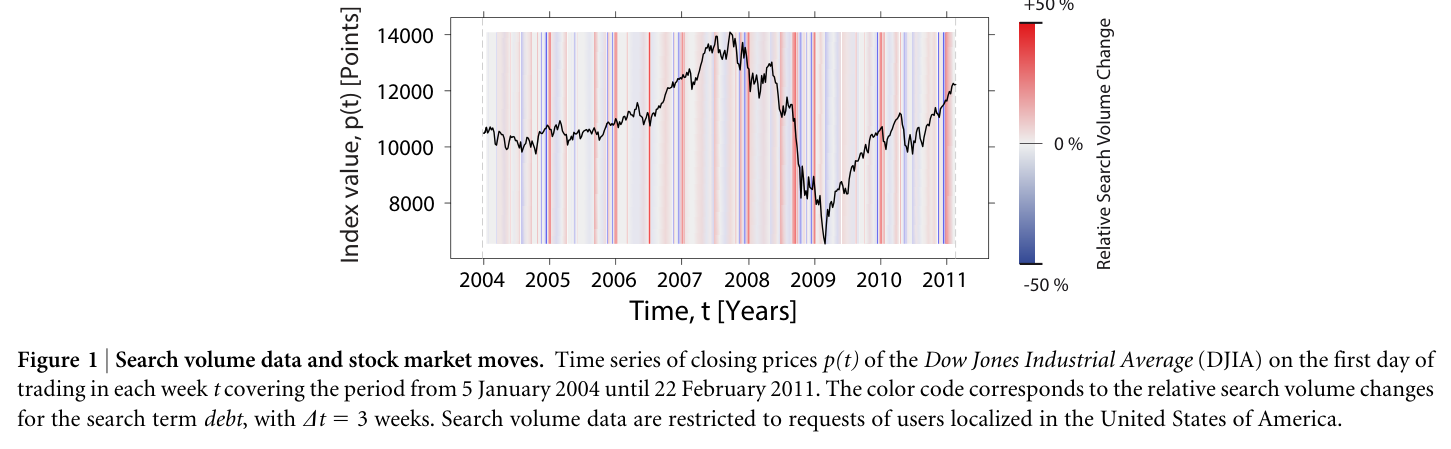
\includegraphics[width=0.8\linewidth]{gfx/m4l2_preis_fig1_search_volume_stock_moves.png}
\par\smallskip{\small \textbf{Hình 1:} Dữ liệu khối lượng tìm kiếm và các biến động của thị trường chứng khoán. Chuỗi thời gian giá đóng cửa $p(t)$ của chỉ số công nghiệp trung bình Dow Jones (DJIA) vào ngày giao dịch đầu tiên của mỗi tuần $t$, trong giai đoạn từ ngày 5 tháng 1 năm 2004 đến ngày 22 tháng 2 năm 2011. Mã màu tương ứng với sự thay đổi tương đối của khối lượng tìm kiếm đối với từ khóa \emph{debt}, với $\Delta t = 3$ tuần. Dữ liệu khối lượng tìm kiếm được giới hạn ở các yêu cầu tìm kiếm của người dùng tại Hoa Kỳ.}
\end{figure}

Để làm sáng tỏ mối quan hệ giữa khối lượng truy vấn tìm kiếm đối với một từ khóa cụ thể và hướng đi chung trong quyết định của nhà giao dịch, chúng tôi phân tích giá đóng cửa $p(t)$ của chỉ số DJIA vào ngày giao dịch đầu tiên của tuần $t$. Chúng tôi sử dụng Google Trends để xác định số lượt tìm kiếm $n(t-1)$ đã được thực hiện đối với một từ khóa cụ thể, chẳng hạn như \emph{debt}, trong tuần $t-1$ (Google định nghĩa một tuần kết thúc vào ngày Chủ nhật), tính theo tỷ lệ so với tổng số lượt tìm kiếm được thực hiện trên Google trong khoảng thời gian đó. Chúng tôi nhận thấy rằng dữ liệu khối lượng tìm kiếm thay đổi nhẹ theo thời gian do quy trình trích xuất của Google. Do đó, đối với mỗi từ khóa tìm kiếm, chúng tôi lấy trung bình của ba lần thực hiện chuỗi thời gian khối lượng tìm kiếm của từ khóa đó, dựa trên ba yêu cầu dữ liệu độc lập trong các tuần liên tiếp. Sự biến thiên của dữ liệu Google Trends theo các ngày truy cập khác nhau không ảnh hưởng đến kết quả của chúng tôi, và có thể chứng minh rằng dữ liệu này phù hợp với các sự kiện thực tế đã được ghi nhận (xem Hình S1 trong Thông tin Bổ sung).

Để định lượng những thay đổi trong hành vi thu thập thông tin, chúng tôi sử dụng độ thay đổi tương đối của khối lượng tìm kiếm:
$$
\Delta n(t, \Delta t) = n(t) - N(t-1, \Delta t)
$$
với
$$
N(t-1, \Delta t) = \frac{n(t-1) + n(t-2) + \cdots + n(t-\Delta t)}{\Delta t}
$$
trong đó $t$ được đo bằng đơn vị tuần. Trong Hình 1, chúng tôi biểu diễn sự thay đổi tương đối của khối lượng tìm kiếm đối với từ khóa \emph{debt}, cùng với mối quan hệ của nó với giá đóng cửa của DJIA.

Để tìm hiểu xem những thay đổi trong hành vi thu thập thông tin được ghi nhận qua dữ liệu Google Trends có liên quan đến những thay đổi giá cổ phiếu sau đó trong giai đoạn 2004--2011 hay không, chúng tôi xây dựng một chiến lược đầu tư giả định cho một danh mục sử dụng dữ liệu khối lượng tìm kiếm, gọi là ``chiến lược Google Trends'' trong phần tiếp theo. Lợi nhuận chỉ có thể đạt được trong một chiến lược giao dịch nếu ít nhất một số thay đổi tương lai của giá cổ phiếu được dự đoán đúng, đặc biệt là xung quanh các biến động lớn của thị trường. Chúng tôi thực hiện chiến lược này bằng cách bán DJIA tại giá đóng cửa $p(t)$ vào ngày giao dịch đầu tiên của tuần $t$, nếu $\Delta n(t-1, \Delta t) > 0$, và mua lại DJIA tại giá $p(t+1)$ vào cuối ngày giao dịch đầu tiên của tuần kế tiếp. Lưu ý rằng có tồn tại các cơ chế cho phép bán tài sản trên thị trường tài chính mà không cần sở hữu tài sản đó trước. Ngược lại, nếu $\Delta n(t-1, \Delta t) < 0$, chúng tôi mua DJIA tại giá đóng cửa $p(t)$ vào ngày giao dịch đầu tiên của tuần $t$ và bán DJIA tại giá $p(t+1)$ vào cuối ngày giao dịch đầu tiên của tuần tiếp theo. Tại thời điểm bắt đầu giao dịch, chúng tôi đặt giá trị của tất cả các danh mục ở một mức tùy ý là 1. Nếu chúng tôi thực hiện một vị thế bán khống (short position), tức bán tại giá đóng cửa $p(t)$ và mua lại tại giá $p(t+1)$, thì lợi suất tích lũy $R$ thay đổi một lượng $\log(p(t)) - \log(p(t+1))$. Nếu chúng tôi thực hiện một vị thế mua (long position), tức mua tại giá đóng cửa $p(t)$ và bán tại giá $p(t+1)$, thì lợi suất tích lũy $R$ thay đổi một lượng $\log(p(t+1)) - \log(p(t))$. Theo cách này, các hành động mua và bán có tác động đối xứng lên lợi suất tích lũy $R$ của danh mục thuộc một chiến lược. Khi sử dụng cách tiếp cận này để phân tích mối quan hệ giữa khối lượng tìm kiếm Google và các biến động của thị trường chứng khoán, chúng tôi bỏ qua phí giao dịch, vì số lượng giao dịch tối đa mỗi năm khi sử dụng chiến lược của chúng tôi chỉ là 104, cho phép một giao dịch đóng và một giao dịch mở mỗi tuần. Dĩ nhiên, chúng tôi không phủ nhận rằng các loại phí giao dịch như vậy sẽ ảnh hưởng đến lợi nhuận trong một lần triển khai thực tế.

Trong Hình 2, hiệu suất của chiến lược Google Trends dựa trên từ khóa \emph{debt} được biểu diễn bằng đường màu xanh lam, trong khi các đường nét đứt thể hiện độ lệch chuẩn của lợi suất tích lũy từ một chiến lược trong đó chúng tôi mua và bán chỉ số thị trường theo cách ngẫu nhiên, không tương quan (``chiến lược đầu tư ngẫu nhiên''). Độ lệch chuẩn này được suy ra từ các mô phỏng của 10,000 lần thực hiện độc lập của chiến lược đầu tư ngẫu nhiên. Hình 2 cho thấy việc sử dụng chiến lược Google Trends, dựa trên từ khóa \emph{debt} với $\Delta t = 3$ tuần, sẽ làm tăng giá trị của một danh mục lên 326\%. Hiệu suất của các chiến lược Google Trends dựa trên tất cả các từ khóa tìm kiếm khác mà chúng tôi phân tích được trình bày trong Hình S3--S100 của Thông tin Bổ sung.

\begin{figure}[H]
\centering
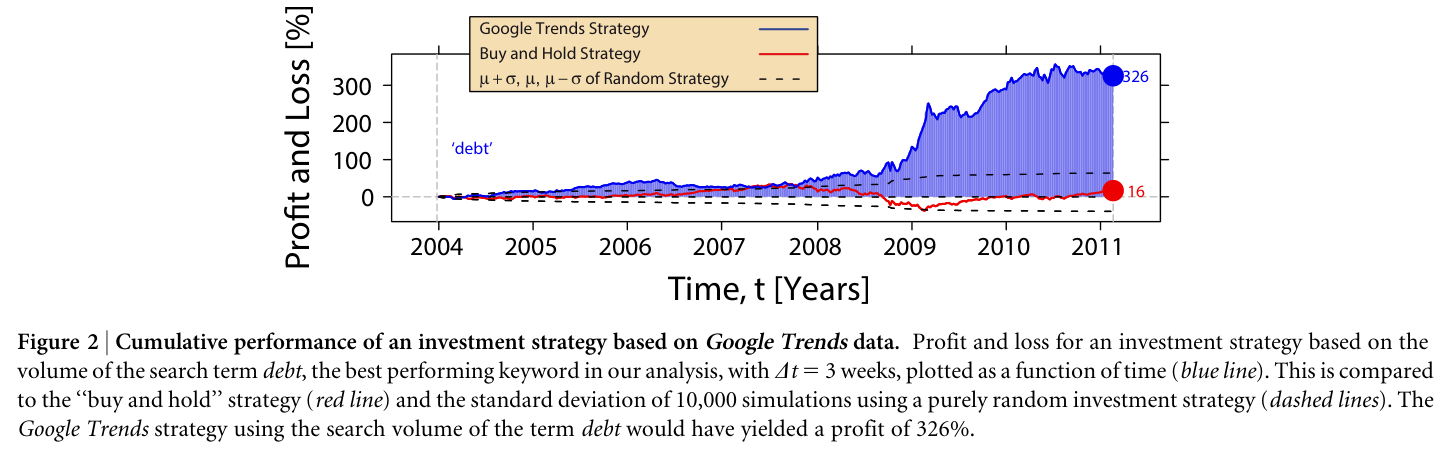
\includegraphics[width=0.8\linewidth]{gfx/m4l2_preis_fig2_cumulative_performance_strategy.png}
\par\smallskip{\small \textbf{Hình 2:} Hiệu suất tích lũy của một chiến lược đầu tư dựa trên dữ liệu Google Trends. Lãi và lỗ của một chiến lược đầu tư dựa trên khối lượng tìm kiếm của từ khóa \emph{debt}, từ khóa cho hiệu suất tốt nhất trong phân tích của chúng tôi, với $\Delta t = 3$ tuần, được biểu diễn theo thời gian (đường màu xanh lam). Kết quả này được so sánh với chiến lược ``mua và nắm giữ'' (đường màu đỏ) và độ lệch chuẩn của 10,000 mô phỏng sử dụng một chiến lược đầu tư hoàn toàn ngẫu nhiên (các đường nét đứt). Chiến lược Google Trends sử dụng khối lượng tìm kiếm của từ khóa \emph{debt} sẽ mang lại lợi nhuận 326\%.}
\end{figure}

Chúng tôi xếp hạng toàn bộ danh sách 98 từ khóa tìm kiếm được nghiên cứu theo hiệu suất giao dịch của chúng khi sử dụng dữ liệu tìm kiếm chỉ của người dùng Hoa Kỳ (Hình 3A) và khi sử dụng dữ liệu khối lượng tìm kiếm được tạo ra trên toàn cầu (Hình 3B). Để đảm bảo tính vững chắc của kết quả, hiệu suất tổng thể của một chiến lược dựa trên một từ khóa tìm kiếm nhất định được xác định là giá trị trung bình của sáu lợi suất thu được với $\Delta t = 1, \ldots, 6$ tuần. Lợi suất của các chiến lược được tính bằng logarit của các thay đổi tương đối trong giá trị danh mục, theo định nghĩa thông thường về lợi suất. Phân bố các giá trị danh mục cuối cùng thu được từ các chiến lược đầu tư ngẫu nhiên gần với phân bố log chuẩn. Do đó, lợi suất tích lũy từ chiến lược đầu tư ngẫu nhiên, được suy ra từ logarit của các giá trị danh mục này, tuân theo phân bố chuẩn, với giá trị trung bình $\langle R \rangle_{\text{RandomStrategy}} = 0$. Ở đây, chúng tôi báo cáo $R$, lợi suất tích lũy của một chiến lược, theo đơn vị độ lệch chuẩn của lợi suất tích lũy của các chiến lược đầu tư ngẫu nhiên không tương quan này.

Chúng tôi nhận thấy rằng lợi suất từ các chiến lược Google Trends mà chúng tôi kiểm định nhìn chung cao hơn đáng kể so với lợi suất từ các chiến lược ngẫu nhiên ($\langle R \rangle_{US} = 0.60$; $t = 8.65$, $df = 97$, $p < 0.001$, kiểm định t một mẫu).

Chúng tôi so sánh hiệu suất của các từ khóa tìm kiếm này với hai chiến lược tham chiếu. Chiến lược ``mua và nắm giữ'' được thực hiện bằng cách mua chỉ số ngay từ đầu và bán ra vào cuối giai đoạn nắm giữ. Chiến lược này mang lại lợi nhuận 16\%, bằng đúng mức tăng tổng thể của giá trị DJIA trong giai đoạn từ tháng 1 năm 2004 đến tháng 2 năm 2011. Chúng tôi tiếp tục xây dựng một ``chiến lược Dow Jones'' bằng cách sử dụng các thay đổi trong $p(t)$ thay cho các thay đổi trong dữ liệu khối lượng tìm kiếm làm cơ sở cho các quyết định mua và bán. Chúng tôi nhận thấy rằng chiến lược này cũng chỉ mang lại 33\% lợi nhuận với $\Delta t = 3$ tuần, hay khi được xác định là giá trị trung bình của sáu lợi suất thu được với $\Delta t = 1, \ldots, 6$ tuần thì tương đương 0.45 độ lệch chuẩn của lợi suất tích lũy của các chiến lược đầu tư ngẫu nhiên không tương quan (Hình 3A và 3B; xem thêm Hình S101 trong Thông tin Bổ sung).

\begin{figure}[H]
\centering
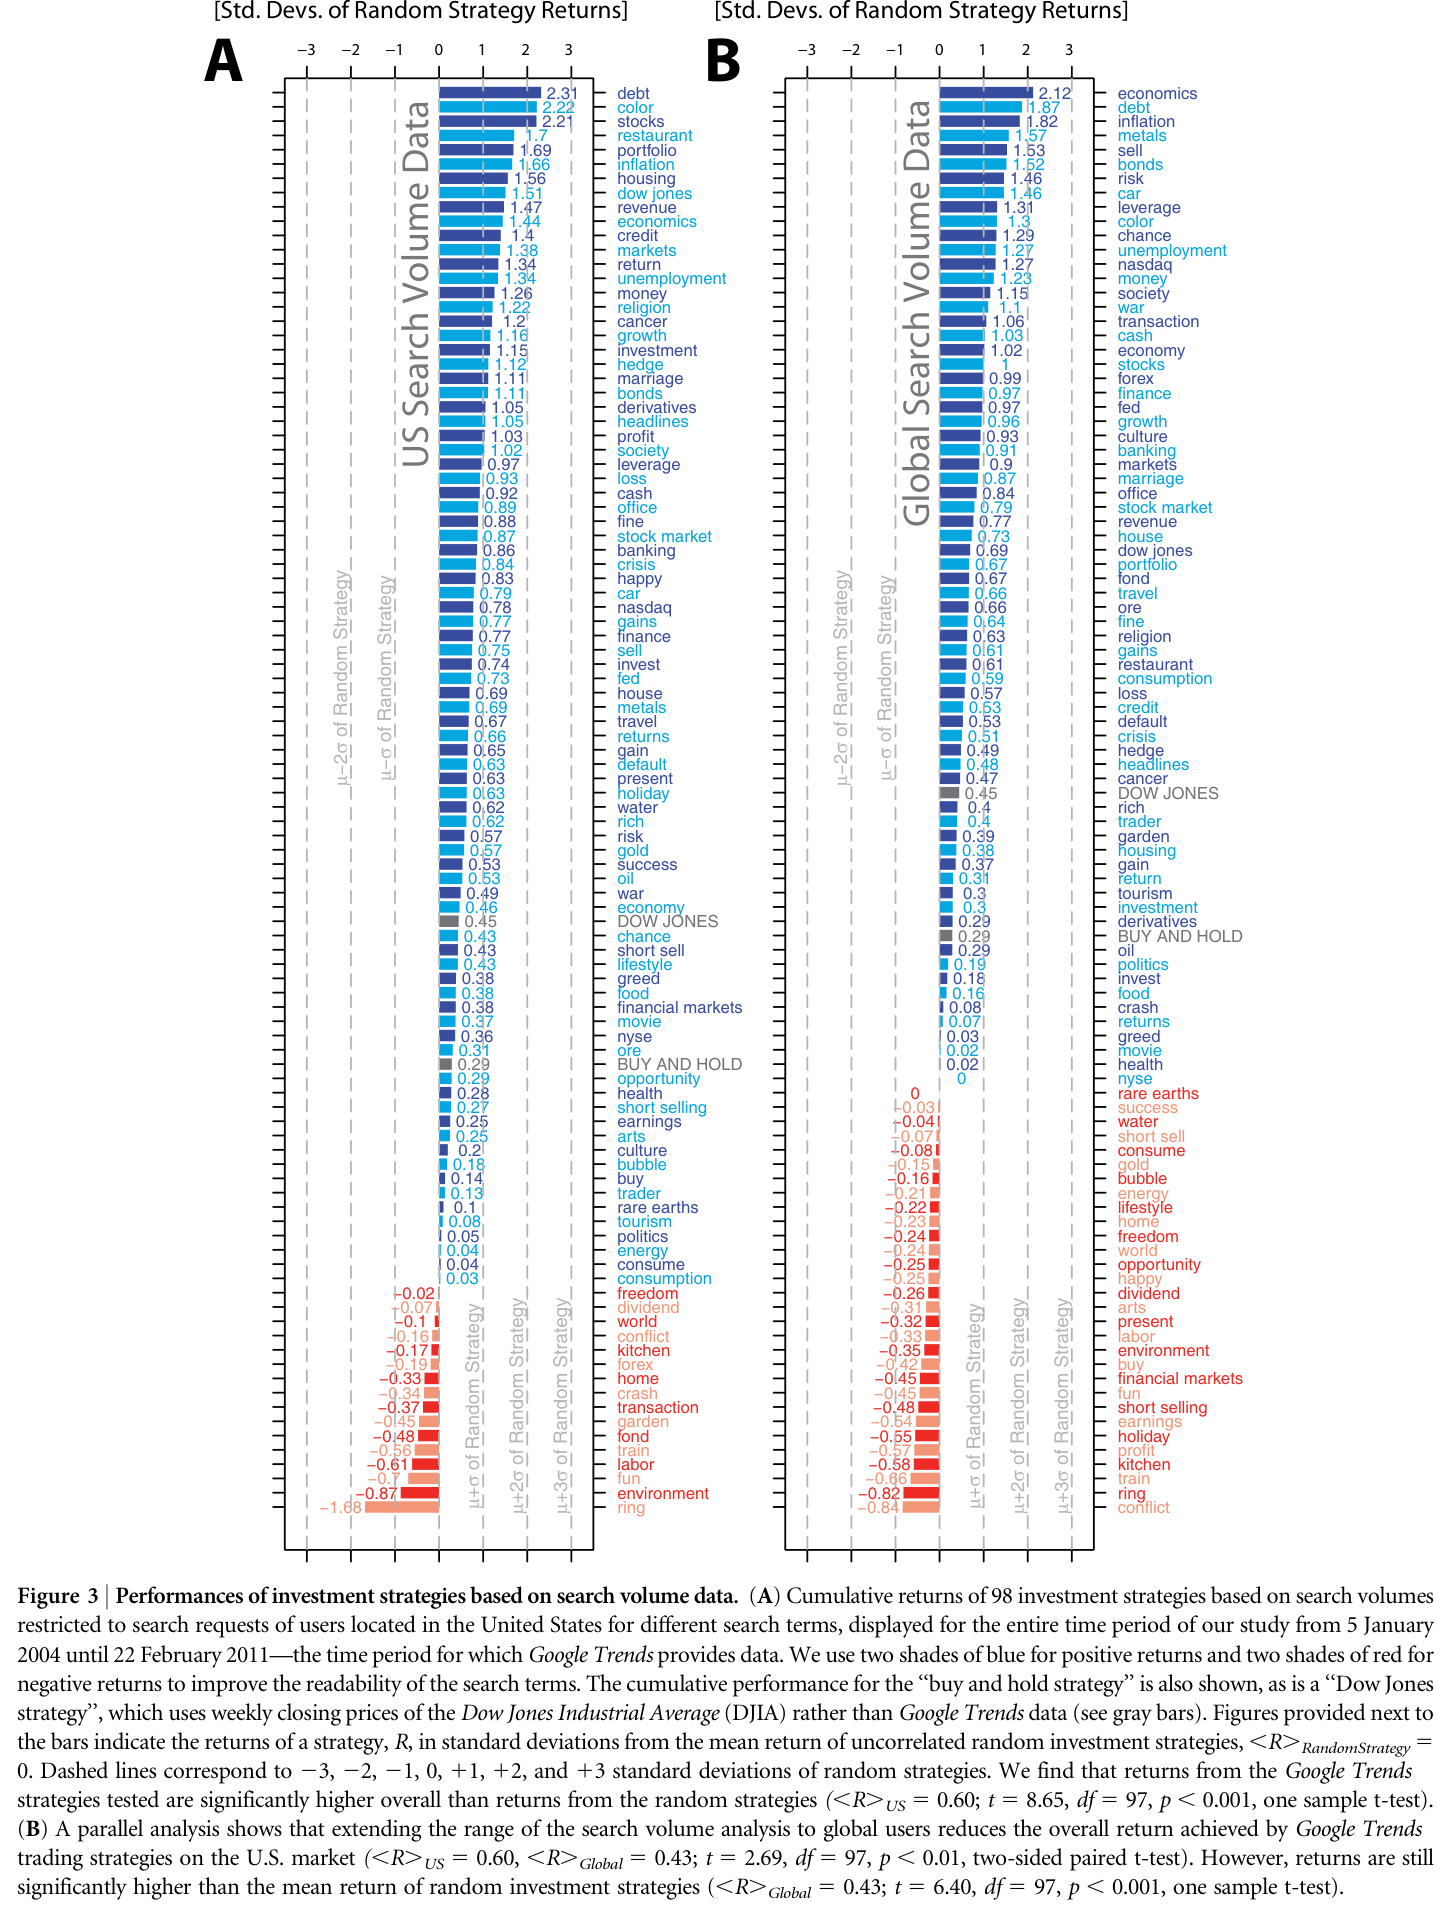
\includegraphics[width=0.8\linewidth]{gfx/m4l2_preis_fig3_performances_search_volume_strategies.png}
\par\smallskip{\small \textbf{Hình 3:} Hiệu suất của các chiến lược đầu tư dựa trên dữ liệu khối lượng tìm kiếm. (A) Lợi suất tích lũy của 98 chiến lược đầu tư dựa trên khối lượng tìm kiếm, giới hạn ở các yêu cầu tìm kiếm của người dùng tại Hoa Kỳ đối với các từ khóa tìm kiếm khác nhau, được trình bày cho toàn bộ giai đoạn nghiên cứu từ ngày 5 tháng 1 năm 2004 đến ngày 22 tháng 2 năm 2011, giai đoạn mà Google Trends cung cấp dữ liệu. Chúng tôi sử dụng hai sắc độ xanh lam cho lợi suất dương và hai sắc độ đỏ cho lợi suất âm nhằm cải thiện khả năng đọc của các từ khóa tìm kiếm. Hiệu suất tích lũy của chiến lược ``mua và nắm giữ'' cũng được trình bày, cùng với ``chiến lược Dow Jones'', chiến lược sử dụng giá đóng cửa hàng tuần của DJIA thay vì dữ liệu Google Trends (xem các thanh màu xám). Các số liệu bên cạnh các thanh thể hiện lợi suất của một chiến lược, $R$, theo đơn vị độ lệch chuẩn so với lợi suất trung bình của các chiến lược đầu tư ngẫu nhiên không tương quan, $\langle R \rangle_{\text{RandomStrategy}} = 0$. Các đường nét đứt tương ứng với $-3, -2, -1, 0, +1, +2$ và $+3$ độ lệch chuẩn của các chiến lược ngẫu nhiên. Chúng tôi nhận thấy rằng lợi suất từ các chiến lược Google Trends được kiểm định nhìn chung cao hơn đáng kể so với lợi suất từ các chiến lược ngẫu nhiên ($\langle R \rangle_{US} = 0.60$; $t = 8.65$, $df = 97$, $p < 0.001$, kiểm định t một mẫu). (B) Một phân tích song song cho thấy việc mở rộng phạm vi phân tích khối lượng tìm kiếm sang người dùng toàn cầu làm giảm lợi suất tổng thể đạt được bởi các chiến lược giao dịch Google Trends trên thị trường Hoa Kỳ ($\langle R \rangle_{US} = 0.60$, $\langle R \rangle_{\text{Global}} = 0.43$; $t = 2.69$, $df = 97$, $p < 0.01$, kiểm định t bắt cặp hai phía). Tuy nhiên, lợi suất vẫn cao hơn đáng kể so với lợi suất trung bình của các chiến lược đầu tư ngẫu nhiên ($\langle R \rangle_{\text{Global}} = 0.43$; $t = 6.40$, $df = 97$, $p < 0.001$, kiểm định t một mẫu).}
\end{figure}

Kết quả của chúng tôi cho thấy hiệu suất của chiến lược Google Trends khác nhau tùy theo từ khóa tìm kiếm được chọn. Chúng tôi tìm hiểu xem liệu những khác biệt về hiệu suất này có thể được giải thích một phần bằng một chỉ báo về mức độ liên quan tài chính của các từ khóa khác nhau hay không, một khái niệm mà chúng tôi định lượng bằng cách tính tần suất xuất hiện của mỗi từ khóa tìm kiếm trên ấn bản trực tuyến của tờ \emph{Financial Times} từ tháng 8 năm 2004 đến tháng 6 năm 2011, được chuẩn hóa theo số kết quả tìm kiếm Google (Google hits) của mỗi từ khóa (xem Hình S2 trong Thông tin Bổ sung). Chúng tôi nhận thấy rằng lợi suất gắn với một từ khóa tìm kiếm nhất định có tương quan với chỉ báo mức độ liên quan tài chính này, sử dụng hệ số tương quan hạng tau của Kendall ($\tau = 0.275$, $z = 4.01$, $N = 98$, $p < 0.001$).

Người ta thường công nhận rằng nhà đầu tư có xu hướng ưu tiên giao dịch trên thị trường trong nước của họ, cho thấy rằng dữ liệu tìm kiếm chỉ của người dùng Hoa Kỳ, như đã sử dụng trong các phân tích trên, sẽ nắm bắt hành vi thu thập thông tin của những người tham gia thị trường chứng khoán Hoa Kỳ tốt hơn so với dữ liệu của người dùng Google trên toàn cầu. Thật vậy, chúng tôi nhận thấy rằng các chiến lược dựa trên dữ liệu khối lượng tìm kiếm toàn cầu kém thành công hơn so với các chiến lược dựa trên dữ liệu khối lượng tìm kiếm của Hoa Kỳ trong việc dự đoán các biến động của thị trường Hoa Kỳ ($\langle R \rangle_{US} = 0.60$, $\langle R \rangle_{\text{Global}} = 0.43$; $t = 2.69$, $df = 97$, $p < 0.01$, kiểm định t bắt cặp hai phía).

Các kết quả thực nghiệm của chúng tôi cho đến nay phù hợp với một giả thuyết gồm hai phần: cụ thể là những đợt tăng giá quan trọng của DJIA được báo trước bởi sự sụt giảm khối lượng tìm kiếm đối với một số từ khóa liên quan đến tài chính nhất định, và ngược lại, những đợt giảm giá quan trọng của DJIA được báo trước bởi sự gia tăng khối lượng tìm kiếm đối với một số từ khóa liên quan đến tài chính nhất định. Tuy nhiên, chiến lược giao dịch của chúng tôi có thể được phân tách thành hai thành phần chiến lược: một thành phần trong đó sự sụt giảm khối lượng tìm kiếm thúc đẩy chúng tôi mua vào (hay nắm giữ vị thế mua), và một thành phần trong đó sự gia tăng khối lượng tìm kiếm thúc đẩy chúng tôi bán ra (hay nắm giữ vị thế bán khống).

Để xác minh rằng cả hai thành phần chiến lược đều đóng vai trò quan trọng trong kết quả của chúng tôi, sao cho chúng tôi có bằng chứng cho cả hai phần của giả thuyết này, chúng tôi xây dựng và kiểm định một chiến lược trong đó chúng tôi chỉ nắm giữ vị thế mua sau khi khối lượng tìm kiếm sụt giảm và không bao giờ nắm giữ vị thế bán khống (Hình 4A), và một chiến lược khác trong đó chúng tôi chỉ nắm giữ vị thế bán khống sau khi khối lượng tìm kiếm gia tăng và không bao giờ nắm giữ vị thế mua (Hình 4B). Chúng tôi nhận thấy rằng lợi suất từ cả hai thành phần của chiến lược Google Trends đều cao hơn đáng kể so với lợi suất từ một chiến lược đầu tư ngẫu nhiên (các chiến lược vị thế mua: $\langle R \rangle_{\text{USLong}} = 0.41$; $t = 11.42$, $df = 97$, $p < 0.001$, kiểm định t một mẫu; các chiến lược vị thế bán khống: $\langle R \rangle_{\text{USShort}} = 0.19$; $t = 5.28$, $df = 97$, $p < 0.001$, kiểm định t một mẫu).

\begin{figure}[H]
\centering
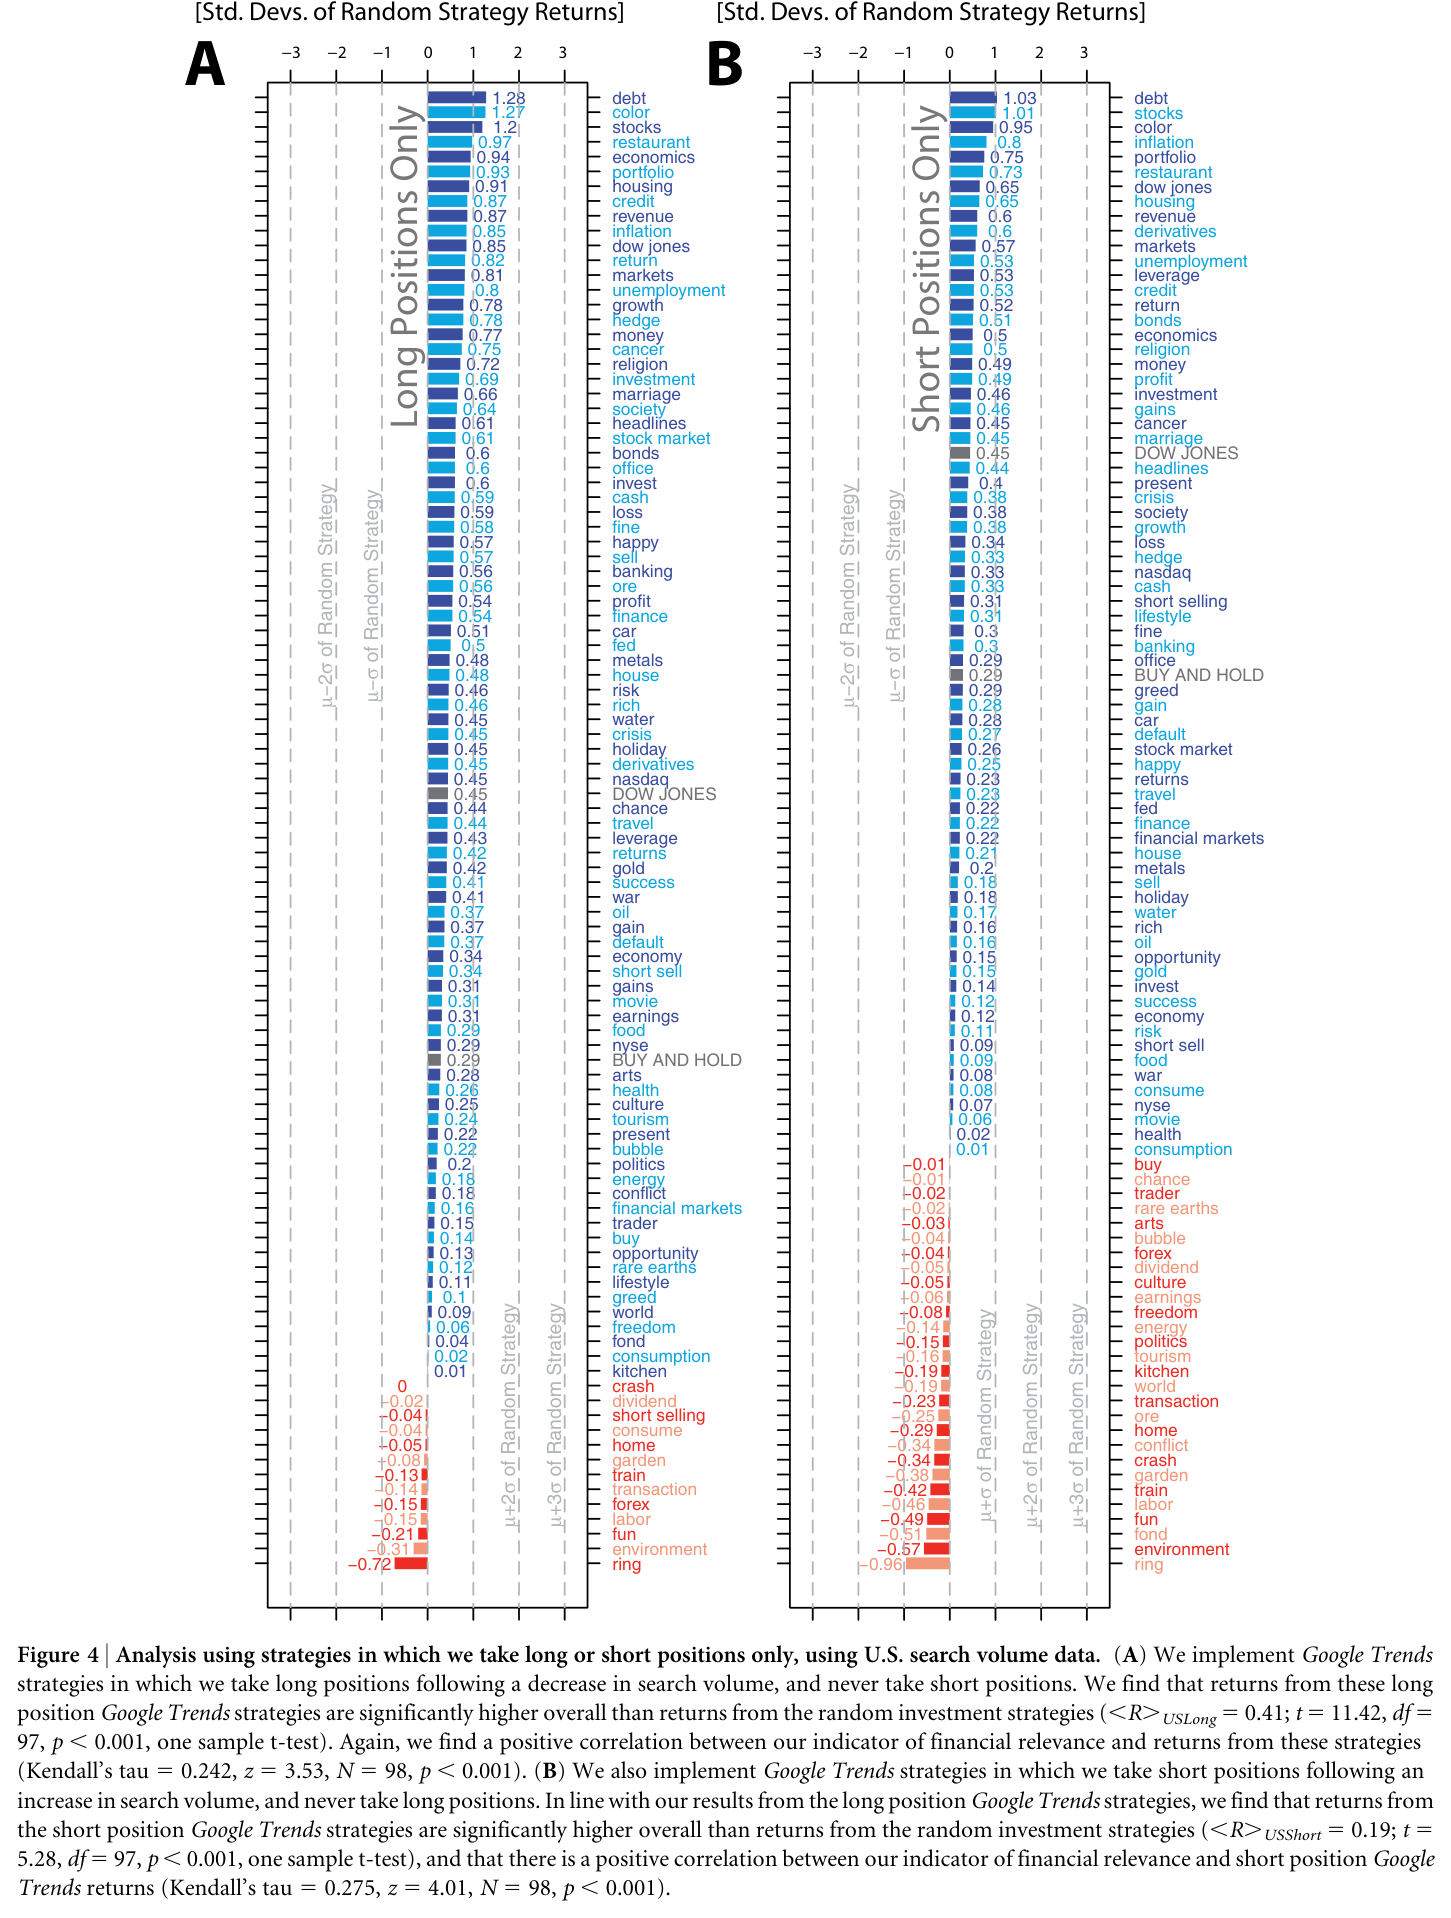
\includegraphics[width=0.8\linewidth]{gfx/m4l2_preis_fig4_long_short_positions_analysis.png}
\par\smallskip{\small \textbf{Hình 4:} Phân tích sử dụng các chiến lược chỉ nắm giữ vị thế mua hoặc vị thế bán khống, sử dụng dữ liệu khối lượng tìm kiếm của Hoa Kỳ. (A) Chúng tôi xây dựng các chiến lược Google Trends trong đó chúng tôi nắm giữ vị thế mua sau một đợt sụt giảm khối lượng tìm kiếm, và không bao giờ nắm giữ vị thế bán khống. Chúng tôi nhận thấy rằng lợi suất từ các chiến lược Google Trends chỉ nắm giữ vị thế mua này nhìn chung cao hơn đáng kể so với lợi suất từ các chiến lược đầu tư ngẫu nhiên ($\langle R \rangle_{\text{USLong}} = 0.41$; $t = 11.42$, $df = 97$, $p < 0.001$, kiểm định t một mẫu). Một lần nữa, chúng tôi tìm thấy mối tương quan dương giữa chỉ báo mức độ liên quan tài chính của chúng tôi và lợi suất từ các chiến lược này (tau Kendall $= 0.242$, $z = 3.53$, $N = 98$, $p < 0.001$). (B) Chúng tôi cũng xây dựng các chiến lược Google Trends trong đó chúng tôi nắm giữ vị thế bán khống sau một đợt gia tăng khối lượng tìm kiếm, và không bao giờ nắm giữ vị thế mua. Phù hợp với kết quả từ các chiến lược Google Trends chỉ nắm giữ vị thế mua, chúng tôi nhận thấy rằng lợi suất từ các chiến lược Google Trends chỉ nắm giữ vị thế bán khống này nhìn chung cao hơn đáng kể so với lợi suất từ các chiến lược đầu tư ngẫu nhiên ($\langle R \rangle_{\text{USShort}} = 0.19$; $t = 5.28$, $df = 97$, $p < 0.001$, kiểm định t một mẫu), và có mối tương quan dương giữa chỉ báo mức độ liên quan tài chính của chúng tôi và lợi suất vị thế bán khống Google Trends (tau Kendall $= 0.275$, $z = 4.01$, $N = 98$, $p < 0.001$).}
\end{figure}

\section{Thảo luận}

Tóm lại, kết quả của chúng tôi phù hợp với gợi ý rằng trong giai đoạn nghiên cứu, dữ liệu Google Trends không chỉ phản ánh các khía cạnh của trạng thái hiện tại của nền kinh tế, mà còn có thể cung cấp một số hiểu biết về các xu hướng tương lai trong hành vi của các chủ thể kinh tế. Sử dụng dữ liệu lịch sử từ giai đoạn tháng 1 năm 2004 đến tháng 2 năm 2011, chúng tôi phát hiện sự gia tăng khối lượng tìm kiếm Google đối với các từ khóa liên quan đến thị trường tài chính trước các đợt sụt giảm của thị trường chứng khoán. Kết quả của chúng tôi cho thấy những dấu hiệu cảnh báo này trong dữ liệu khối lượng tìm kiếm có thể đã được khai thác để xây dựng các chiến lược giao dịch có lợi nhuận.

Chúng tôi đưa ra một cách diễn giải khả dĩ cho kết quả của mình trong khuôn khổ mô hình ra quyết định của Herbert Simon. Chúng tôi cho rằng dữ liệu Google Trends và dữ liệu thị trường chứng khoán có thể phản ánh hai giai đoạn kế tiếp nhau trong quá trình ra quyết định của nhà đầu tư. Xu hướng bán ra trên thị trường tài chính ở mức giá thấp hơn có thể được báo trước bởi các giai đoạn lo ngại. Trong những giai đoạn lo ngại như vậy, con người có thể có xu hướng thu thập thêm thông tin về trạng thái của thị trường. Có thể hình dung rằng hành vi như vậy trước đây có thể đã được phản ánh qua sự gia tăng khối lượng tìm kiếm Google Trends đối với các từ khóa có mức độ liên quan tài chính cao hơn.

Chúng tôi nhận thấy rằng các chiến lược dựa trên dữ liệu khối lượng tìm kiếm của người dùng Hoa Kỳ thành công hơn đối với thị trường Hoa Kỳ so với các chiến lược sử dụng dữ liệu khối lượng tìm kiếm toàn cầu. Với giả định rằng nhóm người dùng Internet tại Hoa Kỳ có tỷ lệ nhà giao dịch trên thị trường Hoa Kỳ cao hơn so với nhóm người dùng Internet trên toàn thế giới, phát hiện này phù hợp với gợi ý thú vị rằng các tập dữ liệu này có thể cung cấp những hiểu biết về các giai đoạn ra quyết định khác nhau trong cùng một nhóm dân số.

Trong công trình này, chúng tôi đưa ra một sự định lượng về mối quan hệ giữa những thay đổi trong khối lượng tìm kiếm và những thay đổi trong giá thị trường chứng khoán. Các nghiên cứu trong tương lai sẽ cần thiết để đưa ra một giải thích thấu đáo về các cơ chế tâm lý nền tảng khiến con người tìm kiếm các từ khóa như \emph{debt} trước khi bán cổ phiếu ở mức giá thấp hơn. Rõ ràng vẫn còn nhiều cơ hội để mở rộng các phân tích của chúng tôi sang các tập dữ liệu tài chính khác.

Kết quả nghiên cứu của chúng tôi cho thấy rằng việc kết hợp các tập dữ liệu hành vi quy mô lớn, chẳng hạn như dữ liệu giao dịch tài chính, với dữ liệu về khối lượng truy vấn tìm kiếm, có thể mở ra những hiểu biết mới về các giai đoạn khác nhau của quá trình ra quyết định tập thể quy mô lớn. Chúng tôi kết luận rằng những kết quả này tiếp tục minh họa cho những khả năng thú vị mà các tập dữ liệu lớn mới mang lại nhằm nâng cao hiểu biết của chúng ta về hành vi tập thể phức tạp trong xã hội.

\section{Phương pháp}

Các từ khóa tìm kiếm liên quan đến chủ đề tài chính ở mức độ nào? Chúng tôi định lượng mức độ liên quan tài chính bằng cách tính tần suất xuất hiện của mỗi từ khóa tìm kiếm trên ấn bản trực tuyến của tờ \emph{Financial Times} (\url{http://www.ft.com}) từ tháng 8 năm 2004 đến tháng 6 năm 2011, được chuẩn hóa theo số kết quả tìm kiếm Google (Google hits, \url{http://www.google.com}) của mỗi từ khóa. Chi tiết được trình bày trong Thông tin Bổ sung.

\textbf{Thu thập dữ liệu.} Chúng tôi thu thập dữ liệu khối lượng tìm kiếm bằng cách truy cập trang web Google Trends (\url{http://www.google.com/trends}) vào các ngày 10 tháng 4 năm 2011, 17 tháng 4 năm 2011 và 24 tháng 4 năm 2011. Dữ liệu về số kết quả tìm kiếm của các từ khóa trên ấn bản trực tuyến của tờ \emph{Financial Times} được thu thập vào ngày 7 tháng 6 năm 2011. Số kết quả tìm kiếm Google (Google hits) cho các từ khóa này được thu thập vào ngày 8 tháng 6 năm 2011.

\section{Lời cảm ơn và thông tin bổ sung}

\textbf{Lời cảm ơn.} Chúng tôi xin cảm ơn Didier Sornette, Dirk Helbing và Steven R. Bishop vì những góp ý của họ. Công trình này được tài trợ một phần bởi Quỹ Nghiên cứu Đức (German Research Foundation), khoản tài trợ PR 1305/1-1 (cho T.P.). Công trình này cũng được hỗ trợ bởi Cơ quan Hoạt động Nghiên cứu Tình báo Tiên tiến (Intelligence Advanced Research Projects Activity, IARPA) thông qua hợp đồng số D12PC00285 của Trung tâm Kinh doanh Quốc gia thuộc Bộ Nội vụ Hoa Kỳ (Department of Interior National Business Center, DoI/NBC), cũng như bởi Quỹ Khoa học Quốc gia (National Science Foundation, NSF), Văn phòng Nghiên cứu Hải quân (Office of Naval Research, ONR) và Cơ quan Giảm thiểu Đe dọa Quốc phòng (Defense Threat Reduction Agency, DTRA). Chính phủ Hoa Kỳ được phép sao chép và phân phối các bản in lại cho các mục đích của Chính phủ, bất kể chú thích bản quyền nào trên đó. Tuyên bố miễn trừ trách nhiệm: các quan điểm và kết luận trong tài liệu này là của các tác giả và không nên được diễn giải là nhất thiết đại diện cho các chính sách hoặc sự chứng thực chính thức, dù được nêu rõ hay ngụ ý, của IARPA, DoI/NBC, hay Chính phủ Hoa Kỳ.

\textbf{Đóng góp của tác giả.} T.P., H.S.M. và H.E.S. đã xây dựng thiết kế nghiên cứu, thực hiện các phân tích, thảo luận về kết quả, và đóng góp vào nội dung của bản thảo.

\textbf{Thông tin bổ sung.} Thông tin bổ sung đi kèm bài báo này tại \url{http://www.nature.com/scientificreports}.

\textbf{Xung đột lợi ích tài chính.} Các tác giả tuyên bố không có xung đột lợi ích tài chính nào.

\textbf{Giấy phép.} Công trình này được cấp phép theo Giấy phép Creative Commons Attribution-NonCommercial-ShareAlike 3.0 Unported. Để xem bản sao của giấy phép này, truy cập \url{http://creativecommons.org/licenses/by-nc-sa/3.0/}.

\textbf{Cách trích dẫn bài báo này:} Preis, T., Moat, H.S. \& Stanley, H.E. Quantifying Trading Behavior in Financial Markets Using Google Trends. \emph{Sci. Rep.} 3, 1684; DOI:10.1038/srep01684 (2013).

% [Đã lược bỏ danh mục Tài liệu tham khảo gốc (tiếng Anh, trích dẫn của tác giả bài gốc) để giảm dung lượng chương; không ảnh hưởng nội dung học thuật chính.]

\chapter{Đọc thêm 2: Dự đoán Thị trường Tài chính bằng Google Trends (Challet \& Bel)}
\label{ch:M4L2DT2}

% Nguồn: Challet, D., & Bel, A. ``Predicting financial markets with Google Trends and not so random keywords.'' arXiv, 2014.
% Phần cần đọc: Toàn bộ bài báo
% Nội dung bắt buộc đọc: được kiểm tra trong mọi bài đánh giá (kể cả Quiz).

\section{Thông tin nguồn}

\begin{itemize}
  \item \textbf{Nguồn:} Challet, Damien, and Ahmed Bel Hadj Ayed. \emph{Predicting financial markets with Google Trends and not so random keywords}. arXiv, 2014. \url{https://doi.org/10.48550/arXiv.1307.4643}
  \item \textbf{Phần cần đọc:} Toàn bộ nội dung
\end{itemize}

\bigskip

\noindent\textit{Tác giả: Damien Challet (Chaire de finance quantitative, Laboratoire de mathématiques appliquées aux systèmes, École Centrale Paris, Grande Voie des Vignes, 92295 Châtenay-Malabry, Pháp; và Encelade Capital SA, Parc Scientifique C, EPFL, 1015 Lausanne, Thụy Sĩ) và Ahmed Bel Hadj Ayed (cùng chi nhánh École Centrale Paris nêu trên).}

\section{Tóm tắt}

Chúng tôi thảo luận về những tuyên bố cho rằng dữ liệu từ Google Trends chứa đủ thông tin để dự đoán lợi suất chỉ số tài chính trong tương lai. Trước tiên, chúng tôi rà soát nhiều sai lệch tinh vi (và ít tinh vi hơn) có thể ảnh hưởng đến việc kiểm định lùi (backtest) một chiến lược giao dịch, đặc biệt khi chiến lược đó dựa trên loại dữ liệu này. Như dự đoán, việc lựa chọn từ khóa đóng vai trò then chốt: bằng cách sử dụng một hệ thống backtest đạt chuẩn công nghiệp, chúng tôi xác nhận rằng các từ khóa ngẫu nhiên liên quan đến tài chính không chứa nhiều thông tin dự đoán có thể khai thác hơn so với các từ khóa ngẫu nhiên liên quan đến bệnh tật, xe cổ và trò chơi thùng (arcade games). Tuy nhiên, các từ khóa khác khi áp dụng lên những tài sản phù hợp lại tạo ra các chiến lược giao dịch có lợi nhuận ổn định, qua đó xác nhận trực giác (intuition) của tài liệu tham khảo [24].

\section{I. Giới thiệu}

Việc đo lường nhịp đập của xã hội với tần suất và độ chính xác chưa từng có đang trở nên khả thi nhờ dữ liệu từ nhiều trang web khác nhau. Cụ thể, dữ liệu từ Google Trends (viết tắt là GT trong bài này) báo cáo mức độ quan tâm tìm kiếm (search volume interest, SVI) trong lịch sử đối với các từ khóa cho trước và đã được dùng để dự đoán hiện tại [7] (được gọi là \emph{nowcasting} trong [5]), nghĩa là để cải thiện ước tính các đại lượng đang hình thành nhưng số liệu của chúng chỉ được công bố vào cuối một giai đoạn nhất định. Các đại lượng này bao gồm số liệu thất nghiệp, du lịch và niềm tin tiêu dùng [7], lợi nhuận hàng quý của doanh nghiệp (từ các lượt tìm kiếm về sản phẩm chủ lực của họ) [8], ước tính Tổng sản phẩm quốc nội (GDP) [5] và dịch cúm [15].

Các nhà giao dịch xác định giá tài sản. Một số nhà giao dịch tìm kiếm, chia sẻ và cuối cùng tạo ra thông tin trên nhiều trang web khác nhau. Do đó, giá tài sản lẽ ra phải liên quan đến hành vi của người dùng website. Phép tam đoạn luận này đã được nghiên cứu chi tiết trong [9]: lợi suất giá của các cổ phiếu thành phần trong chỉ số Russell 3000 được hồi quy theo nhiều nhân tố, bao gồm dữ liệu GT, và các nhân tố này được lấy trung bình trên toàn bộ 3000 tài sản. Trong số các phát hiện khác, các tác giả nhận thấy một mối tương quan đáng kể giữa những thay đổi trong SVI và hoạt động giao dịch của nhà đầu tư cá nhân. Ngoài ra, tính trung bình, các biến động của SVI có tương quan âm với lợi suất giá trong khoảng vài tuần trong giai đoạn được nghiên cứu (tức là trong mẫu, in-sample). Nhu cầu lấy trung bình trên nhiều cổ phiếu xuất phát từ lượng nhiễu trong cả lợi suất giá lẫn dữ liệu GT, và từ việc chỉ một phần nhỏ những người tìm kiếm một từ khóa cho trước thực sự giao dịch sau đó.

Tuyên bố của [24] mạnh mẽ hơn nhiều: bài báo cho rằng lợi suất tương lai của chỉ số Dow Jones Industrial Average có tương quan âm với các bất ngờ SVI (SVI surprise) liên quan đến một số từ khóa nhất định, do đó dữ liệu GT chứa đủ thông tin để dự đoán các chỉ số tài chính. Một số sai lệch tinh vi (và không quá tinh vi) khiến kết luận của họ không thể mạnh mẽ như đáng lẽ phải có. Bằng cách sử dụng một hệ thống backtest chặt chẽ, chúng tôi có thể xác nhận rằng dữ liệu GT có thể được dùng để dự đoán lợi suất giá tài sản trong tương lai, qua đó đặt kết luận của họ trên một nền tảng vững chắc hơn nhiều.

\section{II. Dữ liệu và Chiến lược}

Giá tài sản thô được mô tả khá tốt bởi các bước đi ngẫu nhiên (random walk) phù hợp, vốn hoàn toàn không chứa khả năng dự đoán. Tuy nhiên, giá tài sản có thể trở nên dự đoán được nếu người ta có thể xác định một tập hợp điều kiện, sử dụng hoặc chỉ lợi suất tài sản (xem ví dụ [21] về các điều kiện dựa trên tương quan chéo giữa các tài sản) hoặc các nguồn thông tin bên ngoài. Google Trends cung cấp các chuỗi thời gian đã chuẩn hóa về số lượt tìm kiếm cho các từ khóa cho trước với độ phân giải thời gian theo tuần [28], ký hiệu là $v_t$. [24] đề xuất chiến lược giao dịch sau: định nghĩa mức độ quan tâm tìm kiếm cơ sở (baseline) trước đó là
$$
\bar v_t = \frac{1}{T}\sum_{t'=t-T}^{t} v_{t'},
$$
bất ngờ SVI (SVI surprise) là $\delta_t = v_t - \bar v_{t-1}$, và vị thế cần nắm giữ trên tài sản liên quan trong tuần $t+1$ là $s_{t+1} = -\text{sign}\,\delta_t$. Không có gì ngăn cản việc xem xét chiến lược nghịch đảo, nhưng hiện tượng đảo chiều giá trung bình (price reversion) trong một hoặc hai tuần tiếp theo tương ứng với một thay đổi của SVI đã được các tác giả khác ghi nhận trước đó [9, 11].

Thay vì cố gắng dự đoán chỉ số Dow Jones Industrial Average, chúng tôi sử dụng chuỗi thời gian của SPY, vốn phản ánh chỉ số Standard and Poor's 500. Điều này cung cấp một hình thức kiểm định chéo (cross-validation) yếu, vì hai chuỗi thời gian này có tương quan cao nhưng không hoàn toàn đồng nhất. Vì cùng lý do đó, chúng tôi tính lợi suất từ giá đóng cửa thứ Hai đến giá đóng cửa thứ Sáu thay vì từ thứ Hai đến thứ Hai, giúp giữ cho lợi suất chỉ số đồng bộ với dữ liệu GT (dữ liệu này trải dài từ Chủ nhật đến thứ Bảy).

\section{III. Các Sai lệch Phương pháp luận}

Dự đoán vốn đã khó, đặc biệt là dự đoán về tương lai. Nhưng dự đoán về tương lai trong quá khứ còn khó hơn. Điều này đặc biệt đúng với việc backtest một chiến lược giao dịch, tức là việc tính toán lợi nhuận ảo (virtual gains) của chiến lược đó trong quá khứ. Backtest dễ mắc phải nhiều loại sai lệch có thể làm thay đổi đáng kể độ tin cậy của nó, thường theo hướng tích cực (lạc quan hóa kết quả) [14, 20]. Phần lớn các sai lệch này bắt nguồn từ xu hướng đáng tiếc và có lẽ khó tránh khỏi của việc thông tin tương lai len lỏi vào quá khứ.

\subsection*{A. Sai lệch do công cụ}

Đây là sai lệch dễ bị bỏ qua nhất. Nó giải thích một phần lý do vì sao hiệu suất backtest thường rất tốt trong những năm 1980 và 1990, nhưng kém ấn tượng hơn kể từ khoảng năm 2003, ngay cả khi đã tính đến các ước tính thực tế về tổng chi phí giao dịch. Việc tìm ra khả năng dự đoán trong dữ liệu cũ bằng công cụ hiện đại thực sự dễ dàng hơn mức đáng lẽ phải có. Hãy hình dung việc áp dụng các phương pháp tốn nhiều tài nguyên CPU hoặc bộ nhớ lên dữ liệu từ thời kỳ trước khi có máy tính. Định luật nổi tiếng nhất về sự gia tăng năng lực tính toán mang tên Gordon Moore, người nhận thấy rằng số lượng bóng bán dẫn tối ưu trong mạch tích hợp tăng theo hàm mũ theo thời gian (với chu kỳ tăng gấp đôi $\tau \simeq 2$ năm) [23]. Nhưng các khía cạnh quan trọng khác của tính toán cũng đã và đang cải thiện theo hàm mũ, chẳng hạn như lượng tính toán trên mỗi đơn vị năng lượng (định luật Koomey, $\tau \simeq 1.5$ năm [18]) hoặc giá lưu trữ (định luật Kryder, $\tau \simeq 2$ năm [19]). Đáng chú ý, những tiến bộ công nghệ này được phản chiếu qua sự tiến hóa của khung thời gian phản ứng tối thiểu (minimal reaction timescale) trong dữ liệu tài chính [16]. Thêm vào đó, khả năng gần đây có thể huy động và giải phóng gần như tức thì những nguồn lực điện toán đám mây khổng lồ lên các tập dữ liệu lớn đã thay đổi cách thức phân tích dữ liệu tài chính. Rất khó để tính đến sai lệch này. Với mục đích giáo dục, người ta có thể làm quen với năng lực máy tính trong quá khứ bằng các máy ảo như \texttt{qemu} [2], được tinh chỉnh để mô phỏng tốc độ và bộ nhớ của các máy tính sẵn có tại một thời điểm nhất định với một số tiền nhất định.

Loại sai lệch tương tự cũng mở rộng sang những tiến bộ trong tài liệu thống kê và học máy, và thậm chí cả cách người ta hiểu về động lực học thị trường: việc sử dụng một phương pháp cụ thể có khả năng cho kết quả tốt hơn trước khi phương pháp đó được công bố so với, chẳng hạn, một hoặc hai năm sau đó. Người ta có thể mở rộng lập luận này sang tính lịch sử của các phương pháp được kiểm định trên dữ liệu tài chính tại bất kỳ thời điểm nào, bởi vì chúng đi theo trào lưu (fashion). Dù sao đi nữa, đây là một khía cạnh của backtest xứng đáng được nghiên cứu một cách hệ thống hơn.

\subsection*{B. Sai lệch dữ liệu}

Dữ liệu bị sai lệch theo hai cách. Thứ nhất, khi backtest một chiến lược phụ thuộc vào các tín hiệu bên ngoài, trước tiên người ta phải tự hỏi liệu tín hiệu đó có thực sự sẵn có vào các thời điểm mà nó ghi nhận hay không. Dữ liệu GT không sẵn có một cách đáng tin cậy trước ngày 6 tháng 8 năm 2008, vì khi đó dữ liệu chỉ được cập nhật một cách ngẫu nhiên vài tháng một lần [27]. Các backtest tại những thời điểm trước đó chứa đựng một phần khoa học viễn tưởng không thể tránh khỏi, nhưng vẫn hữu ích để hiệu chỉnh (calibrate) các chiến lược.

Vấn đề thứ hai là dữ liệu bị điều chỉnh lại (revised) vì nhiều lý do. Dữ liệu tài chính thô thường chứa các sai sót nghiêm trọng (giá hoặc khối lượng bị lỗi hoặc thiếu, v.v.), nhưng đây chính là dữ liệu mà người ta đáng lẽ đã phải sử dụng trong quá khứ. Dữ liệu lịch sử được tải về sau này thường đã được làm sạch một phần. [10] đưa ra những lời khuyên hữu ích về việc làm sạch dữ liệu tần suất cao. Việc điều chỉnh lại cũng rất phổ biến đối với dữ liệu vĩ mô. Ví dụ, các ước tính GDP được điều chỉnh nhiều lần trước khi đạt đến con số chính thức cuối cùng (về khả năng dự đoán của việc điều chỉnh, xem ví dụ [13]).

Một cách trớ trêu hơn, việc điều chỉnh dữ liệu còn bao gồm cả thay đổi định dạng: loại dữ liệu mà GT trả về đã được điều chỉnh vào cuối năm 2012. Trước đây, dữ liệu gồm các số thực với cách chuẩn hóa không hoàn toàn minh bạch; dữ liệu cũng đi kèm với độ bất định (uncertainty) trên các con số này. Một cách khá nhất quán, bản thân các con số sẽ thay đổi trong phạm vi sai số cho trước mỗi khi người ta tải lại dữ liệu cho cùng một từ khóa. Ngày nay, GT trả về các số nguyên trong khoảng từ 0 đến 100, với 100 là giá trị lớn nhất và 0 là giá trị nhỏ nhất của chuỗi thời gian; những thay đổi nhỏ trong dữ liệu GT do đó bị che khuất bởi quá trình làm tròn; các khoảng sai số không còn khả dụng nữa, nhưng có thể coi hợp lý rằng một biến động $\pm 1$ nên được xem là không đáng kể. Nhân tiện, quá trình làm tròn các chữ số thập phân cuối cùng của giá đôi khi tạo ra khả năng dự đoán giả tạo (spurious predictability), điều đã được biết rõ đối với dữ liệu ngoại hối (FX) [17].

\begin{table}[H]
\centering
\begin{tabular}{|l|c||l|c||l|c||l|c|}
\hline
Từ khóa & t-stat & Từ khóa & t-stat & Từ khóa & t-stat & Từ khóa & t-stat \\
\hline
\texttt{multiple sclerosis} & $-2.1$ & \texttt{Chevrolet Impala} & $-1.9$ & \texttt{Moon Buggy} & $-2.1$ & \texttt{labor} & $-1.5$ \\
\texttt{muscle cramps} & $-1.9$ & \texttt{Triumph 2000} & $-1.9$ & \texttt{Bubbles} & $-2.0$ & \texttt{housing} & $-1.2$ \\
\texttt{premenstrual syndrome} & $-1.8$ & \texttt{Jaguar E-type} & $-1.7$ & \texttt{Rampage} & $-1.7$ & \texttt{success} & $-1.2$ \\
\texttt{alopecia} & $2.2$ & \texttt{Iso Grifo} & $1.7$ & \texttt{Street Fighter} & $2.3$ & \texttt{bonds} & $1.9$ \\
\texttt{gout} & $2.2$ & \texttt{Alfa Romeo Spider} & $1.7$ & \texttt{Crystal Castles} & $2.4$ & \texttt{Nasdaq} & $2.0$ \\
\texttt{bone cancer} & $2.4$ & \texttt{Shelby GT 500} & $2.4$ & \texttt{Moon Patrol} & $2.7$ & \texttt{investment} & $2.0$ \\
\hline
\end{tabular}
\par\smallskip
{\small \textbf{Bảng I:} Các từ khóa và t-stat tương ứng của hiệu suất một chiến lược đơn giản sử dụng chuỗi thời gian Google Trends để dự đoán giá SPY từ giá đóng cửa thứ Hai đến giá đóng cửa thứ Sáu.}
\end{table}

Việc điều chỉnh dữ liệu cũng liên quan đến vũ trụ tài sản có thể đầu tư (investible universe). Dữ liệu lịch sử được cung cấp miễn phí thường không bao gồm các cổ phiếu đã ngừng niêm yết (deceased stocks). Đây là một vấn đề thực sự vì các tài sản xuất hiện và biến mất với một tốc độ khá đều đặn: tập hợp tài sản có thể đầu tư ngày hôm nay không giống với tập hợp của tuần trước. Theo đó, thành phần của các chỉ số cũng thay đổi. Việc phân tích hành vi của các thành phần hiện tại của một chỉ số trong quá khứ là một cách phổ biến để vô tình nạp thông tin tương lai vào dữ liệu, và do đó có một tên gọi chính thức: sai lệch sống sót (survivorship bias). Sai lệch này được biết là làm lệch đáng kể các thước đo hiệu suất trung bình. Ví dụ, [14] cho thấy sai lệch này gây ra tình trạng ước tính vượt mức (overestimation) hiệu suất backtest trong 90\% các trường hợp danh mục chỉ mua (long-only) trong một giai đoạn được lựa chọn kỹ. Điều này hợp lý vì theo định nghĩa, các công ty đã sống sót là những công ty hoạt động tốt. Những lo ngại ban đầu liên quan đến hiệu suất của các quỹ tương hỗ (mutual funds), và nhiều phương pháp khác nhau đã được đề xuất để ước tính mức độ của sai lệch này dựa trên tỷ lệ sống sót của các quỹ [3, 12].

Cuối cùng, cần lưu ý rằng việc backtest các chiến lược trên những chỉ số không thể giao dịch trực tiếp (untradable indices), chẳng hạn như chỉ số Nasdaq Composite, không phải là một ý tưởng khôn ngoan, vì không ai có thể thực sự cố gắng loại bỏ khả năng dự đoán khỏi các chỉ số này.

\subsection*{C. Lựa chọn từ khóa}

Việc lựa chọn từ khóa nào tất nhiên là một yếu tố then chốt khi sử dụng GT để dự đoán. Có vẻ tự nhiên khi nghĩ rằng các từ khóa liên quan đến tài chính sẽ có nhiều khả năng liên quan đến các chỉ số tài chính hơn, do đó có khả năng dự đoán tốt hơn. Theo hướng đó, [24] xây dựng một danh sách từ khóa lấy từ \emph{Financial Times}, một tạp chí tài chính, với chủ đích thiên lệch tập từ khóa theo hướng này. Nhưng sự thiên lệch (bias) này cần được kiểm soát bằng một tập từ khóa ngẫu nhiên không liên quan đến tài chính, điều mà bài báo đó đã bỏ qua.

Hãy hình dung rằng một từ liên quan đến tài chính là từ có liên quan nhất trong cửa sổ trong mẫu (in-sample window). Bộ não của chúng ta vốn được lập trình sẵn để tìm ra một câu chuyện nhằm giải thích cho hiệu suất tốt có vẻ như vậy. Nhưng thống kê thì không như vậy: để kiểm định xem hiệu suất trung bình của một chiến lược giao dịch có khác 0 hay không, người ta sử dụng kiểm định t (t-test), kết quả của kiểm định này sẽ được gọi là t-stat trong phần tiếp theo, và được định nghĩa là
$$
z = \frac{\mu}{\sigma}\sqrt{N},
$$
trong đó $\mu$ là lợi suất trung bình của chiến lược, $\sigma$ là độ lệch chuẩn của chúng và $N$ là số lượng lợi suất; với $N>20$, $z$ trông rất giống một biến ngẫu nhiên Gauss với trung bình bằng 0 và phương sai bằng 1. [24] đã tính toán t-stat một cách hợp lý: từ khóa tốt nhất, \texttt{debt}, có t-stat bằng 2.3. Từ khóa tốt thứ hai là \texttt{color}, có t-stat bằng 2.2. Cả hai con số này không thể phân biệt được về mặt thống kê, nhưng \texttt{debt} được bàn luận trong bài báo và trên báo chí, còn \texttt{color} thì không, mặc dù có sức mạnh ``dự đoán'' tương đương.

Hãy thử nghiệm với các từ khóa ngẫu nhiên đã được biết đến trước khi giai đoạn backtest bắt đầu (2004). Chúng tôi thu thập dữ liệu GT cho 200 tình trạng/bệnh tật y khoa phổ biến, 100 mẫu xe cổ và 100 trò chơi thùng (arcade games) hay nhất mọi thời đại (được liệt kê trong Phụ lục A) và áp dụng chiến lược mô tả ở trên với $k=10$ thay vì $k=5$. Bảng I báo cáo 3 hiệu suất dương và 3 hiệu suất âm tốt nhất (có thể chuyển thành dương bằng cách đảo ngược quy tắc của chiến lược) cho mỗi tập từ khóa.

Chúng tôi để độc giả tự suy ngẫm xem mình sẽ kết luận gì nếu \texttt{bone cancer} (ung thư xương) hay \texttt{Moon Patrol} có liên quan nhiều hơn đến tài chính. Bảng này cũng minh họa rằng các t-stat tốt nhất được báo cáo trong [24] không khác biệt đáng kể so với những gì người ta có thể thu được một cách ngẫu nhiên: vì các t-stat được báo cáo ở đây phần lớn tương đương với các biến ngẫu nhiên Gauss, người ta kỳ vọng 5\% giá trị tuyệt đối của chúng lớn hơn 1.95, điều này giải thích tại sao các từ khóa như \texttt{color} cũng có t-stat tốt. Cuối cùng, \texttt{debt} không nằm trong ba từ khóa tốt nhất khi áp dụng cho SPY từ thứ Hai đến thứ Sáu: hiệu suất của nó không nổi bật và không ổn định, như sẽ được trình bày chi tiết hơn dưới đây.

Tuy nhiên, các t-stat được báo cáo của các thuật ngữ liên quan đến tài chính có xu hướng thiên lệch về phía giá trị dương, điều này phù hợp với hiện tượng đảo chiều được quan sát trong [9, 11], và với kết quả của Bảng I. Điều này có thể cho thấy chiến lược được đề xuất có khả năng trích xuất được một phần lượng thông tin, dù có thể yếu, chứa trong dữ liệu GT.

\subsection*{D. Lỗi lập trình}

Một cách giải thích khác cho sai lệch này có thể là lỗi lập trình (coding errors) (nhưng thực tế không phải vậy). Việc dự đoán chuỗi thời gian trở nên dễ dàng khi người ta vô tình sử dụng dữ liệu tương lai như dữ liệu hiện tại trong một chương trình, chẳng hạn bằng cách dịch chuyển (shift) chuỗi thời gian không chính xác; mã nguồn chúng tôi đã dùng nằm ở phụ lục. Một cách đơn giản và hiệu quả để tránh vấn đề này là lần lượt thay thế lợi suất giá và dữ liệu bên ngoài (ở đây là GT) bằng các chuỗi thời gian ngẫu nhiên. Nếu backtest vẫn tiếp tục cho hiệu suất dương, thì chắc chắn có lỗi (bug) ở đâu đó trong mã nguồn.

\subsection*{E. Không có giai đoạn ngoài mẫu}

Mục tiêu của [24] có lẽ không phải là cung cấp cho chúng ta một chiến lược giao dịch có lợi nhuận, mà là cố gắng minh họa mối quan hệ giữa các lượt tìm kiếm tập thể và lợi suất tài chính trong tương lai. Tuy nhiên, điều đáng chú ý là không có giai đoạn trong mẫu và ngoài mẫu (in-sample và out-of-sample) nào được xem xét (đây là điều đáng ngạc nhiên nhưng đang ngày càng ít phổ biến hơn trong tài liệu học thuật). Do đó, chúng tôi không thể đánh giá hiệu suất giao dịch của chiến lược được đề xuất, vốn chỉ đánh giá được qua tính vững chắc (robustness) và tính nhất quán ngoài mẫu của nó, hay nói cách khác là qua cả hàm lượng thông tin lẫn tính khả thi của chiến lược. Chúng tôi giới thiệu độc giả đến [20] để có một góc nhìn thú vị về tầm quan trọng của các giai đoạn trong mẫu và ngoài mẫu.

\subsection*{F. Từ khóa đến từ tương lai}

[24] sử dụng các từ khóa được lấy từ các số báo \emph{Financial Times} (FT) trong khoảng từ tháng 8/2004 đến tháng 6/2011, được xác định theo kiểu hồi cứu (ex post). Điều này có nghĩa là các từ khóa từ các số báo năm 2011 được dùng để backtest lợi suất của, chẳng hạn, năm 2004. Do đó, tập từ khóa này đã đưa thông tin về tương lai vào quá khứ. Một giải pháp vững chắc hơn là chỉ sử dụng các số báo FT sẵn có tại thời điểm hoặc trước thời điểm diễn ra đánh giá hiệu suất. Đây là lý do vì sao chúng tôi xem xét các tập từ khóa đã được biết đến trước năm 2004.

\subsection*{G. Hiệu chỉnh tham số / Dò dữ liệu}

Mỗi tập tham số, bao gồm cả từ khóa, xác định một hoặc nhiều chiến lược giao dịch. Việc cố gắng tối ưu hóa các tham số hoặc từ khóa được gọi là dò dữ liệu (data snooping) và tất yếu dẫn đến hiệu suất ngoài mẫu không thỏa đáng. Khi các kết quả backtest được trình bày, người đọc thường không thể biết liệu các kết quả đó có mắc phải data snooping hay không. Một biện pháp khắc phục đơn giản là không động đến một phần dữ liệu lịch sử khi kiểm định chiến lược, rồi sau đó dùng phần dữ liệu đó để đánh giá tính nhất quán của hiệu suất (kiểm định chéo, cross-validation) [14]. Các biện pháp khắc phục tinh vi hơn bao gồm kiểm định thực tế của White (White's reality check) [26] (xem ví dụ [25] cho một ứng dụng của phương pháp này). Data snooping tương đương với việc không có giai đoạn ngoài mẫu, ngay cả khi backtest được thực hiện đúng cách với các giai đoạn trong mẫu và ngoài mẫu trượt (sliding).

Hãy thực hiện một số phép hiệu chỉnh tham số trong mẫu (in-sample). Chiến lược được đề xuất chỉ có một tham số duy nhất khi tài sản tài chính đã được chọn: đó là số bước thời gian dùng để tính đường trung bình trượt (moving average) $\bar v_t$. Hình 1 báo cáo t-stat của hiệu suất gắn với từ khóa \texttt{debt} theo hàm của $k$. Dấu của t-stat tương đối vững chắc trước các thay đổi trong khoảng $k \in \{2,\dots,30\}$, nhưng giá trị điển hình của nó trong khoảng này không đặc biệt nổi bật (nằm giữa 1 và 2). Bây giờ, hãy xét từ khóa tốt nhất tuyệt đối trong bốn tập từ khóa, \texttt{Moon Patrol}. Cả giá trị lẫn khoảng ổn định của t-stat của từ khóa này đều tốt hơn nhiều so với \texttt{debt} (xem Hình 2), nhưng điều này nhiều khả năng chỉ do thuần túy ngẫu nhiên. Do đó, không có lý do gì để tin tưởng một từ khóa này hơn từ khóa kia.

\subsection*{H. Không tính phí giao dịch}

Giả định chi phí trung bình 2 điểm cơ bản (bps, 0.02\%) cho mỗi giao dịch, 104 giao dịch mỗi năm và 8 năm giao dịch (2004-2011), chi phí giao dịch làm giảm hiệu suất gắn với bất kỳ từ khóa nào khoảng 20\%. Một hệ quả tích cực là các giai đoạn có hiệu suất đi ngang khi không tính phí bỗng trở thành các giai đoạn hiệu suất âm khi chi phí giao dịch được tính đến, điều này mang lại những kỳ vọng thực tế hơn. Chi phí liên quan đến chênh lệch giá mua bán (spread) và tác động giá (price impact) cũng nên được đưa vào một backtest đúng đắn.

\begin{figure}[H]
\centering
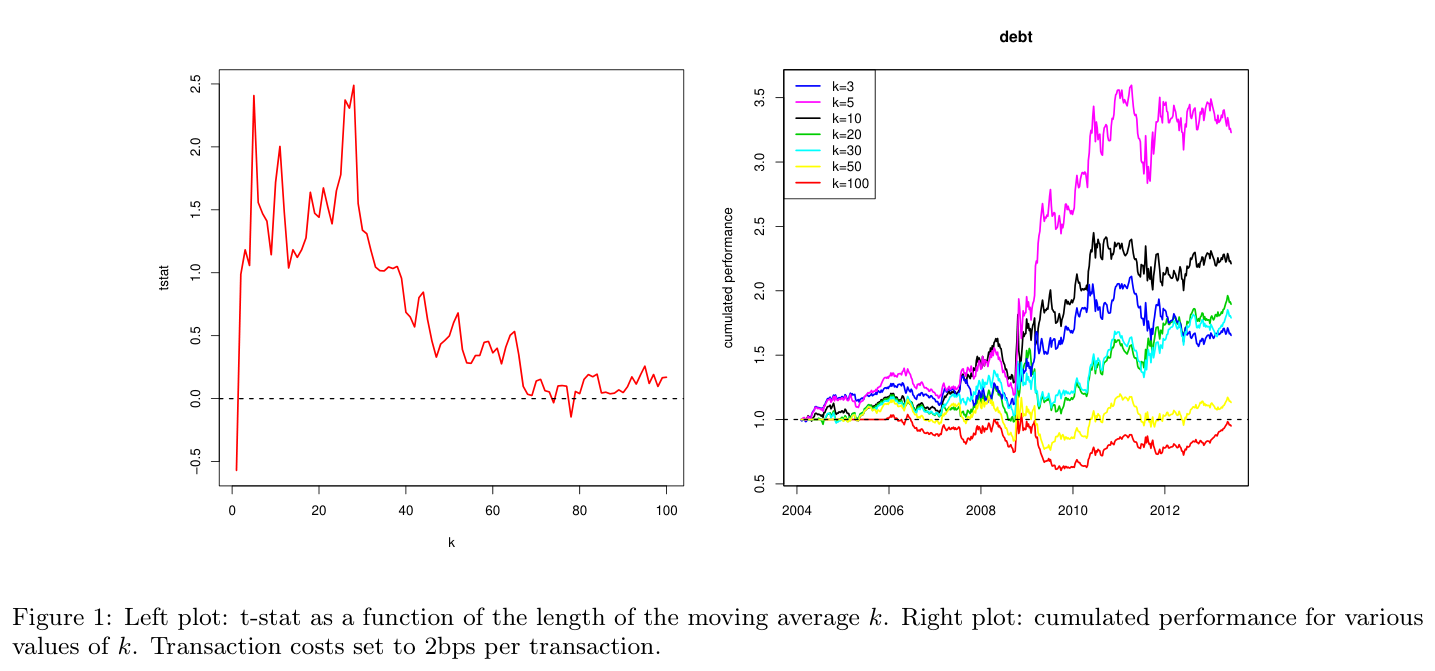
\includegraphics[width=0.8\linewidth]{gfx/m4l2_challetbel_fig1_tstat_vs_movwindow.png}
\par\smallskip{\small \textbf{Hình 1:} Đồ thị trái: t-stat theo hàm của độ dài cửa sổ trượt $k$. Đồ thị phải: hiệu suất tích lũy ứng với các giá trị khác nhau của $k$. Chi phí giao dịch được đặt ở mức 2bps mỗi lần giao dịch.}
\end{figure}

\begin{figure}[H]
\centering
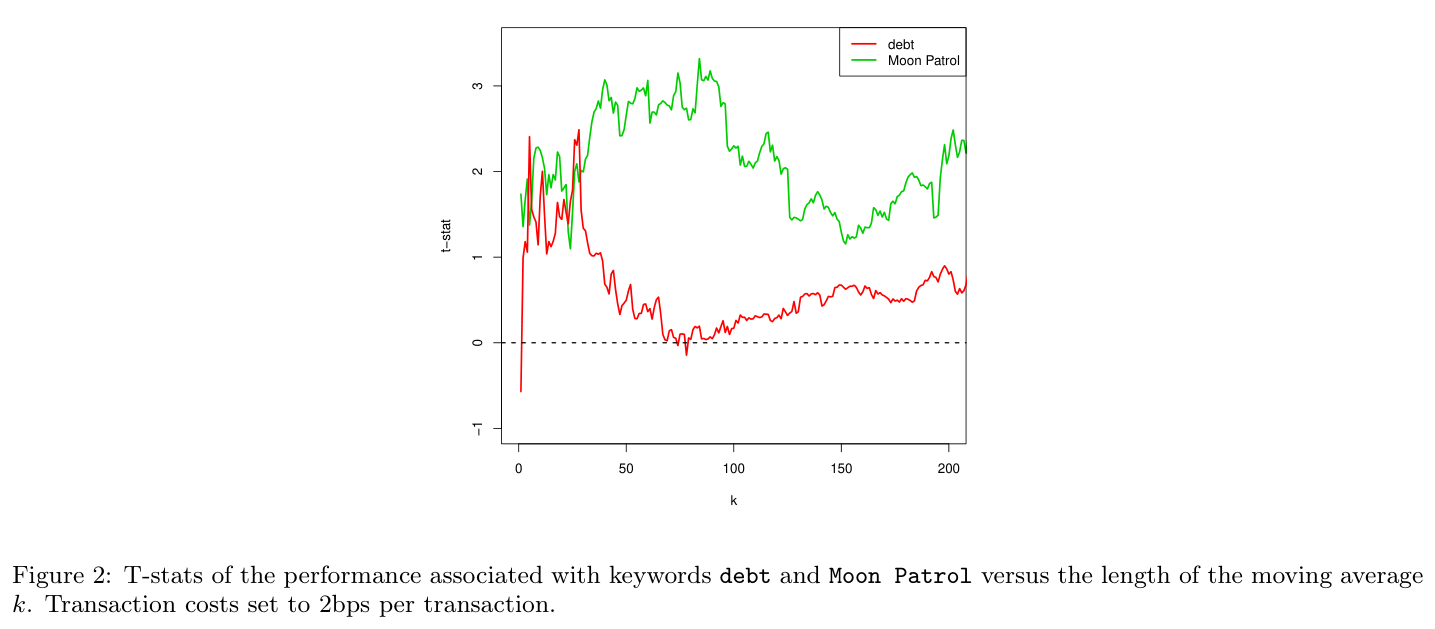
\includegraphics[width=0.8\linewidth]{gfx/m4l2_challetbel_fig2_tstat_debt_moonpatrol.png}
\par\smallskip{\small \textbf{Hình 2:} T-stat của hiệu suất gắn với các từ khóa \texttt{debt} và \texttt{Moon Patrol} theo độ dài của cửa sổ trượt $k$. Chi phí giao dịch được đặt ở mức 2bps mỗi lần giao dịch.}
\end{figure}

\section{IV. Sức Mạnh Dự đoán của Google Trends}

Với nhiều điểm yếu về phương pháp luận đã liệt kê ở trên, người ta có thể bắt đầu nghi ngờ các kết luận của [24]. Ở đây chúng tôi cho thấy rằng các kết luận đó là đúng. Bước đầu tiên là tránh những vấn đề phương pháp luận đã nêu ở trên. Một trong hai tác giả đã dùng một hệ thống backtest đạt chuẩn công nghiệp cùng các chiến lược tinh vi hơn (điều này do đó gây ra sai lệch công cụ). Trước tiên, hãy so sánh hiệu suất tích lũy thu được của ba tập từ khóa ngẫu nhiên mà chúng tôi đã định nghĩa, cộng với tập từ khóa lấy từ \emph{Financial Times}. Đối với mỗi tập từ khóa, chúng tôi chọn làm đầu vào: SVI thô, SVI trễ (lagged), và các đường trung bình trượt khác nhau của SVI, cùng với lợi suất chỉ số trong quá khứ. Kết quả cho thấy không có tập từ khóa nào mang lại thông tin có khả năng dự đoán đáng kể các biến động chỉ số (xem Hình 4). Điều này không mâu thuẫn với kết quả của [9, 11, 24]. Nó chỉ đơn giản có nghĩa là tín hiệu có lẽ quá yếu để có thể khai thác được trong thực tế. Phần cuối của các đường hiệu suất tất nhiên trông hấp dẫn, nhưng điều này xuất phát từ việc lợi suất SPY từ giá đóng cửa thứ Hai đến giá đóng cửa thứ Sáu phần lớn là dương trong giai đoạn này: bất kỳ thuật toán học máy nào chỉ áp dụng trên lợi suất cũng có khả năng cho ra kết quả tương tự.

\begin{figure}[H]
\centering
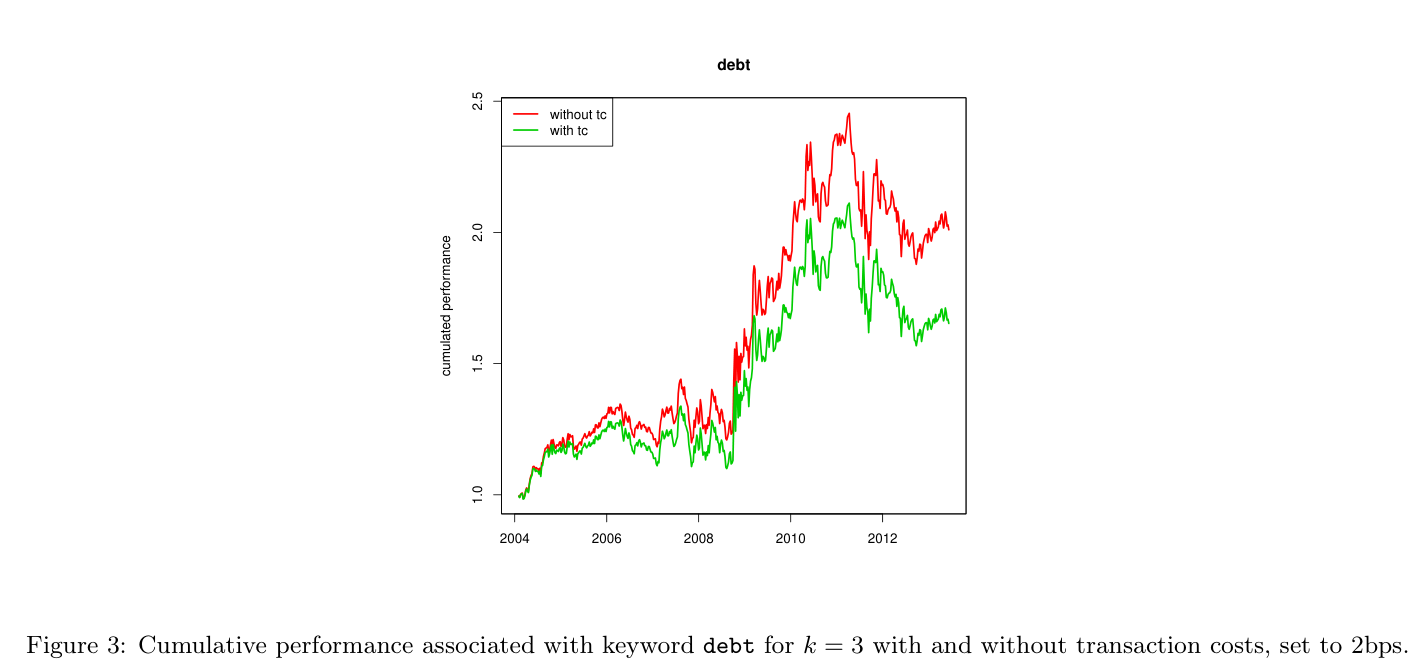
\includegraphics[width=0.6\linewidth]{gfx/m4l2_challetbel_fig3_cumperf_debt_tc.png}
\par\smallskip{\small \textbf{Hình 3:} Hiệu suất tích lũy gắn với từ khóa \texttt{debt} với $k=3$, có và không có chi phí giao dịch, được đặt ở mức 2bps.}
\end{figure}

\begin{figure}[H]
\centering
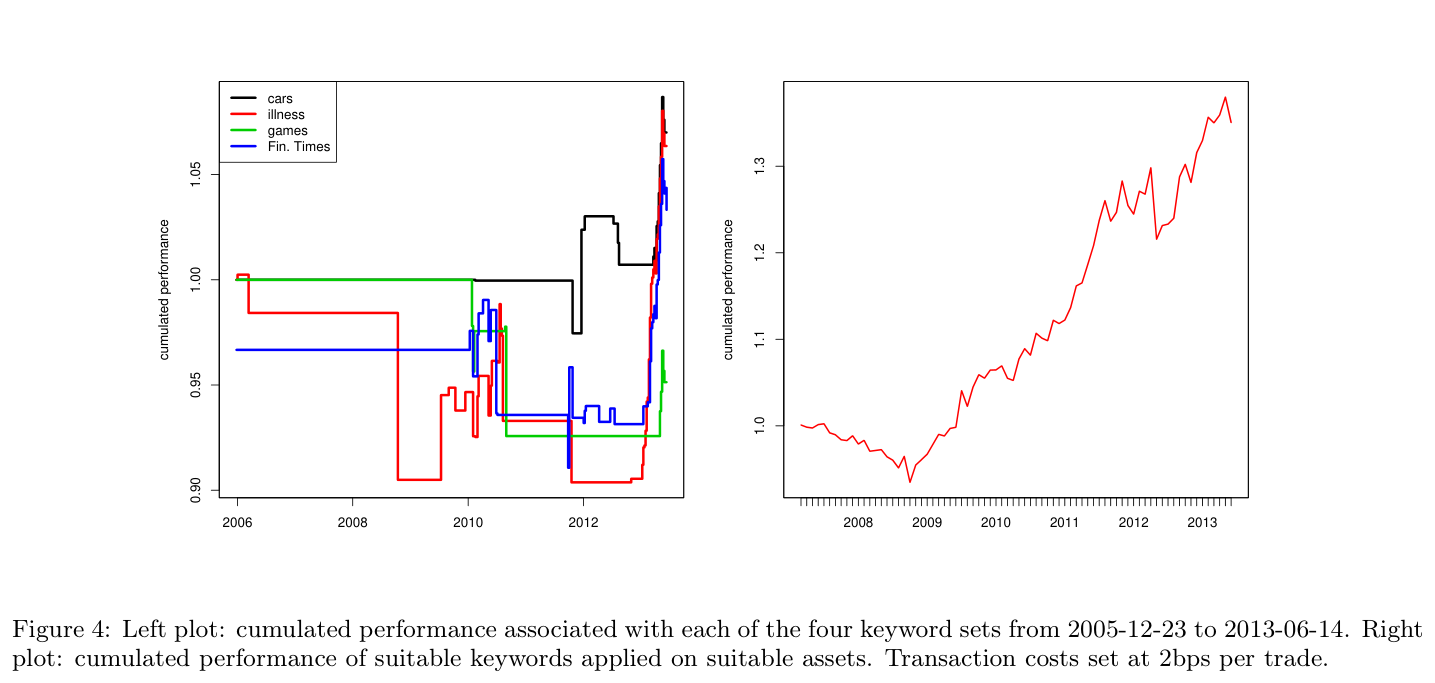
\includegraphics[width=0.8\linewidth]{gfx/m4l2_challetbel_fig4_cumperf_keyword_sets.png}
\par\smallskip{\small \textbf{Hình 4:} Đồ thị trái: hiệu suất tích lũy gắn với từng tập trong bốn tập từ khóa, từ 23/12/2005 đến 14/06/2013. Đồ thị phải: hiệu suất tích lũy của các từ khóa phù hợp áp dụng lên các tài sản phù hợp. Chi phí giao dịch được đặt ở mức 2bps mỗi giao dịch.}
\end{figure}

Cho đến nay, chúng tôi chỉ có thể kết luận rằng một hệ thống backtest đúng đắn (và không quá khắt khe) đã không thể tìm thấy bất kỳ thông tin nào có thể khai thác được từ bốn tập từ khóa, chứ không phải là các tập từ khóa đó không chứa đủ thông tin dự đoán. Để kết luận, chúng tôi sử dụng cùng hệ thống backtest với một số dữ liệu GT, dùng chính xác cùng các tham số và loại đầu vào như trước. Hiệu suất sơ bộ, báo cáo trong Hình 4, hứa hẹn hơn và cho thấy dữ liệu GT thực sự luôn chứa một lượng thông tin dự đoán nhất định. Hiệu suất này không đặc biệt ấn tượng khi so với hiệu suất của chính SPY, nhưng vẫn thú vị vì mức độ tiếp xúc ròng (net exposure) luôn gần bằng 0 (xem [6] để biết thêm thông tin).

\section{V. Thảo luận}

Cần có các phương pháp tinh vi kết hợp với backtest cẩn trọng để chứng minh rằng Google Trends chứa đủ thông tin có thể khai thác được. Điều này là do loại dữ liệu như vậy bao gồm quá nhiều lượt tìm kiếm có lẽ không liên quan đến tài sản tài chính ứng với một từ khóa cho trước, và thậm chí còn ít liên quan hơn nữa đến hoạt động giao dịch thực tế. Khi người ta thu hẹp phạm vi tìm kiếm bằng cách cung cấp nhiều từ khóa hơn, dữ liệu GT thường chỉ chứa thông tin ở quy mô thời gian hàng tháng, hoặc không chứa thông tin nào cả.

Nếu quay lại thuật toán được đề xuất bởi [24] và các phát hiện tương thích của [9, 11], thật khó để hiểu tại sao giá tương lai lại có xu hướng đảo chiều một cách hệ thống sau một bất ngờ SVI dương, và ngược lại một tuần sau đó. Hiện tượng đảo chiều này yếu và chỉ đúng tính trung bình. Đây có thể là kết quả phổ biến nhất, nhưng khả năng sinh lời sẽ cao hơn nhiều nếu người ta biết được điều gì kích hoạt sự đảo chiều hay sự tiếp diễn xu hướng (trend following). Có một số bằng chứng cho thấy việc bổ sung dữ liệu GT bằng tin tức dẫn đến hiệu suất giao dịch được cải thiện đáng kể (xem ví dụ [4]).

Một bài báo khác của cùng nhóm tác giả đề xuất một nguồn thông tin hứa hẹn hơn nhiều: bài báo đó liên hệ những thay đổi trong số lượt truy cập các trang Wikipedia của các công ty cho trước với lợi suất chỉ số trong tương lai [22]. Các nghiên cứu tiếp theo sẽ tìm hiểu sức mạnh dự đoán của loại dữ liệu này.

\section*{Lời cảm ơn}

Chúng tôi xin ghi nhận những cuộc trao đổi hữu ích với Frédéric Abergel, Marouanne Anane và Thierry Bochud.

% [Đã lược bỏ danh mục Tài liệu tham khảo gốc (tiếng Anh, trích dẫn của tác giả bài gốc) để giảm dung lượng chương; không ảnh hưởng nội dung học thuật chính.]

\section*{Phụ lục A: Từ khóa}

Chúng tôi đã tải xuống dữ liệu GT cho các từ khóa sau đây, không qua bất kỳ chỉnh sửa thủ công nào. (Các danh sách từ khóa dưới đây được giữ nguyên bằng tiếng Anh vì đây là các cụm tìm kiếm chính xác đã được dùng để truy vấn Google Trends; việc dịch sang tiếng Việt sẽ làm thay đổi từ khóa thực tế được sử dụng trong bài báo.)

\subsection*{1. Bệnh tật (Illnesses)}

\noindent Nguồn: \url{http://www.ranker.com/list/list-of-common-diseases-most-common-illnesses/diseases-and-medications-info}, truy cập ngày 27 tháng 5 năm 2013.

\smallskip
\noindent\small AIDS, Acne, Acute bronchitis, Allergy, Alopecia, Altitude sickness, Alzheimer's disease, Andropause, Anorexia nervosa, Antisocial personality disorder, Arthritis, Asperger syndrome, Asthma, Attention deficit hyperactivity disorder, Autism, Avoidant personality disorder, Back pain, Bad Breath, Bedwetting, Benign prostatic hyperplasia, Bipolar disorder, Bladder cancer, Bleeding, Body dysmorphic disorder, Bone cancer, Borderline personality disorder, Bovine spongiform encephalopathy, Brain Cancer, Brain tumor, Breast cancer, Burns, Bursitis, Cancer, Canker Sores, Carpal tunnel syndrome, Cervical cancer, Cholesterol, Chronic Childhood Arthritis, Chronic Obstructive Pulmonary Disease, Coeliac disease, Colorectal cancer, Conjunctivitis, Cradle cap, Crohn's disease, Dandruff, Deep vein thrombosis, Dehydration, Dependent personality disorder, Depression, Diabetes mellitus, Diabetes mellitus type 1, Diaper rash, Diarrhea, Disabilities, Dissociative identity disorder, Diverticulitis, Down syndrome, Drug abuse, Dysfunctional uterine bleeding, Dyslexia, Ear Infections, Ear Problems, Eating Disorders, Eczema, Edwards syndrome, Endometriosis, Epilepsy, Erectile dysfunction, Eye Problems, Fibromyalgia, Flu, Fracture, Freckle, Gallbladder Diseases, Gallstone, Gastroesophageal reflux disease, Generalized Anxiety Disorder, Genital wart, Glomerulonephritis, Gonorrhoea, Gout, Gum Diseases, Gynecomastia, HIV, Head Lice, Headache, Hearing impairment, Heart Disease, Heart failure, Heartburn, Heat Stroke, Heel Pain, Hemorrhoid, Hepatitis, Herniated Discs, Herpes simplex, Hiatus hernia, Histrionic personality disorder, Hyperglycemia, Hyperkalemia, Hypertension, Hyperthyroidism, Hypothyroidism, Infectious Diseases, Infectious mononucleosis, Infertility, Influenza, Iron deficiency anemia, Irritable Male Syndrome, Irritable bowel syndrome, Itching, Joint Pain, Juvenile Diabetes, Kidney Disease, Kidney stone, Leukemia, Liver tumour, Lung cancer, Malaria, Melena, Memory Loss, Menopause, Mesothelioma, Migraine, Miscarriage, Mucus In Stool, Multiple sclerosis, Muscle Cramps, Muscle Fatigue, Muscle Pain, Myocardial infarction, Nail Biting, Narcissistic personality disorder, Neck Pain, Obesity, Obsessive-compulsive disorder, Osteoarthritis, Osteomyelitis, Osteoporosis, Ovarian cancer, Pain, Panic attack, Paranoid personality disorder, Parkinson's disease, Penis Enlargement, Peptic ulcer, Peripheral artery occlusive disease, Personality disorder, Pervasive developmental disorder, Peyronie's disease, Phobia, Pneumonia, Poliomyelitis, Polycystic ovary syndrome, Post-nasal drip, Post-traumatic stress disorder, Premature birth, Premenstrual syndrome, Propecia, Prostate cancer, Psoriasis, Reactive attachment disorder, Renal failure, Restless legs syndrome, Rheumatic fever, Rheumatoid arthritis, Rosacea, Rotator Cuff, Scabies, Scars, Schizoid personality disorder, Schizophrenia, Sciatica, Severe acute respiratory syndrome, Sexually transmitted disease, Sinusitis, Skin Eruptions, Skin cancer, Sleep disorder, Smallpox, Snoring, Social anxiety disorder, Staph infection, Stomach cancer, Strep throat, Sudden infant death syndrome, Sunburn, Syphilis, Systemic lupus erythematosus, Tennis elbow, Termination Of Pregnancy, Testicular cancer, Tinea, Tooth Decay, Traumatic brain injury, Tuberculosis, Ulcers, Urinary tract infection, Urticaria, Varicose veins.
\normalsize

\subsection*{2. Xe cổ (Classic cars)}

\noindent Nguồn: \url{http://www.ranker.com/crowdranked-list/the-best-1960_s-cars}, truy cập ngày 27 tháng 5 năm 2013.

\smallskip
\noindent\small 1960 Aston Martin DB4 Zagato, 1960 Ford, 1961 Ferrari 250 SWB, 1961 Ferrari 250GT California, 1963 Corvette, 1963 Iso Griffo A3L, 1964 Ferrari 250 GTL (Lusso), 1965 Bizzarrini 5300 Strada, 1965 Ford GT40, 1965 Maserati Mistral, 1965 Shelby Cobra, 1966 Ferrari 365P, 1966 Maserati Ghibli, 1967 Alfa Romeo Stradale, 1967 Ferrari 275 GTB/4, 1967 Shelby Mustang KR500, 1968 Chevrolet Corvette L88, 1968 DeTomaso Mangusta, 1969 Pontiac Trans Am, 1969 Yenko Chevelle, 57 Chevy, 68 Ferrari 365 GTB/4 Daytona Spyder, 69 Yenko Camaro Z28, AC Cobra, Alfa Romeo Spider, Aston Martin DB5, Austin Mini Saloon 1959, BMW E9, Buick Riviera, Buick Wildcat, Cane, Chevrolet Camaro, Chevrolet Chevelle, Chevrolet Impala, Chevy Chevelle, Chrysler Valiant, Corvette Stingray, Dodge Challenger, Dodge Charger, Dodge Dart Swinger, Facel Vega Facel II, Ferrari 250, Ferrari 250 GTO, Ferrari 275, Ferrari Daytona, Fiat 500, Ford Corsair, Ford Cortina, Ford GT40, Ford Mustang, Ford Ranchero, Ford Thunderbird, Ford Torino, Ford Zephyr MK III, Iso Grifo, Jaguar E-type, Jeep CJ, Lamborghini Miura, Lamborghini Miura SV, Lincoln Continental, Lotus Elan, Maserati Ghibli, Mercedes Benz 220SE, Mercedes-Benz 300SL, Mercury Cougar, Plymouth Barracuda, Pontiac GTO, Porsche 356, Porsche 911, Porsche 911 classic, Shelby GT500, Rambler Classic, Rover 2000, Shelby Daytona Coupe, Shelby GT350, Studebaker Avanti, Sunbeam Tiger, Toyota 2000GT, Triumph 2000, Vauxhall Velox 1960, Vauxhall Victor 1963, Wolseley 15/60.
\normalsize

\subsection*{3. Trò chơi thùng (Arcade Games)}

\noindent Nguồn: \url{http://www.ranker.com/list/list-of-common-diseases-most-common-illnesses/diseases-and-medications-info}, truy cập ngày 27 tháng 5 năm 2013. (Ghi chú của người dịch: đây là URL nguồn được ghi trong bản gốc của bài báo cho danh sách này; có khả năng là một sơ suất trong tài liệu gốc, được giữ nguyên theo đúng bản gốc để không làm sai lệch nội dung.)

\smallskip
\noindent\small 1942, 1943, 720\textdegree{}, After Burner, Airwolf, Altered Beast, Arkanoid, Asteroids, Bad Dudes Vs. DragonNinja, Bagman, Battlezone, Beamrider, Berzerk, Bionic Commando, Bomb Jack, Breakout, Bubble Bobble, Bubbles, BurgerTime, Centipede, Circus Charlie, Commando, Crystal Castles, Cyberball, Dangar - Ufo Robo, Defender, Dig Dug, Donkey Kong, Donkey Kong 3, Donkey Kong Junior, Double Dragon, Dragon's Lair, E.T. (Atari 2600), Elevator Action, Final Fight, Flashback, Food Fight, Frogger, Front Line, Galaga, Galaxian, Gauntlet, Geometry Wars, Gorf, Gyruss, Hogan's Alley, Ikari Warriors, Joust, Kangaroo, Karate Champ, Kid Icarus, Lode Runner, Lunar Lander, Manic Miner, Mappy, Marble Madness, Mario Bros., Millipede, Miner 2049er, Missile Command, Moon Buggy, Moon Patrol, Ms. Pac-Man, Naughty Boy, Pac-Man, Paperboy, Pengo, Pitfall!, Pole Position, Pong, Popeye, Punch-Out!!, Q*bert, Rampage, Red Baron, Robotron: 2084, Rygar: The Legendary Adventure, Sewer Sam, Snow Bros, Space Invaders, Spy Hunter, Star Wars, Stargate, Street Fighter, Super Pac-Man, Tempest, Tetris, The Adventures of Robby Roto!, The Simpsons, Time Pilot, ToeJam \& Earl, Toki, Track \& Field, Tron, Wizard Of Wor, Xevious.
\normalsize

\section*{Phụ lục B: Mã nguồn}

Dưới đây là một cách hiện thực đơn giản bằng ngôn ngữ R cho chiến lược được trình bày trong [24]. Chúng tôi dùng ký hiệu ``='' thay vì ``<-'' để gán giá trị.

\begin{verbatim}
computePerfStats=function(filename,k=10,getPerf=FALSE){
        gtdata=loadGTdata(filename)
        if(is.null(gtdata) || length(gtdata)<100){
                return(NULL)
        }
        spy=loadYahooData('SPY')
        spy_rets=getFutureReturns(spy)        #spy_rets is a zoo object, contains r_{t+1}
        gtdata_mean=rollmeanr(gtdata,k)        # \bar v_t
        gtdata_mean_lagged=lag(gtdata_mean,-1) # \bar v_{t-1}
        pos=2*(gtdata>gtdata_mean_lagged)-1
        perf=-pos*spy_rets
        perf=perf[which(!is.na(perf))]
        if(getPerf){
                return(perf)
        }else{
                return(t.test(perf)$statistic)
        }
}
\end{verbatim}


\chapter{Đọc thêm 3: Mối liên hệ giữa Tiền mã hóa và Sự chú ý trên Google Trends (Aslanidis, Bariviera \& López)}
\label{ch:M4L2DT3}

% Nguồn: Aslanidis, N., Bariviera, A. F., & López, Ó. G. ``The link between cryptocurrencies and Google Trends attention.'' Finance Research Letters, 47, 2022.
% Phần cần đọc: Toàn bộ bài báo
% Nội dung bắt buộc đọc: được kiểm tra trong mọi bài đánh giá (kể cả Quiz).

\section{Thông tin nguồn}

\begin{itemize}
  \item \textbf{Nguồn:} Aslanidis, Nektarios, Aurelio F. Bariviera, and Óscar G. López. \emph{The link between cryptocurrencies and Google Trends attention}. Finance Research Letters, 47, 2022. \url{https://doi.org/10.1016/j.frl.2021.102654}
  \item \textbf{Phần cần đọc:} Toàn bộ nội dung
\end{itemize}

\section{Tóm tắt}

Bài báo này xem xét lại mối liên hệ giữa tiền mã hóa và sở thích được bộc lộ công khai của công chúng, được đo lường gián tiếp thông qua các lượt tìm kiếm trực tuyến. Chúng tôi cho thấy rằng tiền mã hóa không liên quan đến một chỉ số bất định chung như được đo bằng dữ liệu Google Trends của Castelnuovo and Tran (2017). Thay vào đó, tiền mã hóa gắn liền với một thước đo sự chú ý (tìm kiếm) trên Google Trends đặc thù cho thị trường này. Cụ thể, chúng tôi phát hiện một luồng thông tin hai chiều giữa sự chú ý trên Google Trends và lợi suất tiền mã hóa kéo dài đến sáu ngày. Ngoài ra, luồng thông tin từ độ biến động của tiền mã hóa đến sự chú ý trên Google Trends dường như lớn hơn so với chiều ngược lại. Cuối cùng, chúng tôi ghi nhận một sự phụ thuộc đuôi (tail dependence) đáng kể giữa lợi suất tiền mã hóa và Google Trends. Các mối quan hệ này đều đúng đối với năm loại tiền mã hóa được phân tích và các cách kết hợp khác nhau của chỉ số Google Trends Cryptocurrency được đề xuất.

\begin{itemize}
  \item \textbf{Phân loại JEL:} C4, G01, G14
  \item \textbf{Từ khóa:} Tiền mã hóa, Google Trends, Entropy chuyển giao (transfer entropy), Sự chú ý thị trường
\end{itemize}

\section{1. Giới thiệu}

Kể từ khi ra đời năm 2009, Bitcoin đã ngày càng thu hút sự chú ý của các nhà đầu tư, nhà nghiên cứu, tổ chức tài chính và nhà hoạch định chính sách. Những người ủng hộ Bitcoin đầu tiên là những người theo chủ nghĩa tự do cá nhân và những tín đồ thực thụ của tiền mã hóa, những người chỉ trích cuộc khủng hoảng tài chính toàn cầu 2008--2009. Các nhà đầu tư này xem blockchain như một cơ chế để vượt qua hệ thống tài chính truyền thống, vốn bị chỉ trích nặng nề vì quy định lỏng lẻo đã dẫn đến cuộc khủng hoảng nói trên (Karlstrøm, 2014; Dallyn, 2017). Làn sóng thứ hai của những người đam mê Bitcoin là các nhà đầu cơ, những người nhìn thấy ở Bitcoin (và các đồng tiền mã hóa mới phát hành) cơ hội đầu tư với lợi suất cao (Bouoiyour et al., 2015). Làn sóng thứ ba của những người tham gia thị trường là các tổ chức tài chính, vốn muốn đưa công nghệ blockchain vào ngành của mình và cung cấp cho nhà đầu tư các nền tảng đầu tư an toàn hơn (Guo and Liang, 2016; Patki and Sople, 2020). Đồng thời, các chính phủ bắt đầu lo ngại về những tác động tiêu cực tiềm ẩn của tiền mã hóa. Nhiều quốc gia đã ban hành các quy định (ví dụ như luật thuế, luật chống rửa tiền/chống tài trợ khủng bố; xem Global Legal Research Center (2018)) và đưa ra cảnh báo về mức độ rủi ro cao của loại hình đầu tư này (Martin, 2021). Cuối cùng, làn sóng thứ tư của những người tham gia thị trường tiền mã hóa hiện nay liên quan đến các ngân hàng trung ương và các đồng tiền kỹ thuật số của ngân hàng trung ương (Central Bank Digital Currencies) (Fernández-Villaverde et al., 2020; Wang et al., 2021a). Để có một tổng quan chi tiết về sự phát triển và hiện trạng nghiên cứu về tiền mã hóa, chúng tôi giới thiệu độc giả tham khảo Corbet et al. (2019), Bariviera and Merediz-Solà (2021), cùng nhiều nghiên cứu khác.

Đồng thời, quá trình số hóa ngày càng sâu rộng của nền kinh tế đã để lại một dấu vết số mà, theo một cách nào đó, bộc lộ sở thích, thị hiếu hoặc thói quen tiêu dùng. Google Trends đã được chứng minh là hữu ích cho việc dự báo hiện tại (nowcasting) và dự báo các chỉ số kinh tế (Vicente et al., 2015) cũng như dự đoán kết quả chính trị (Mavragani and Tsagarakis, 2016). Vì tiền mã hóa là tài sản có bản chất số hóa ngay từ đầu, nhà đầu tư có xu hướng thu thập thông tin thị trường chủ yếu qua internet (mạng xã hội, diễn đàn chuyên biệt, v.v.). Do đó, các lượt tìm kiếm trên Google có xu hướng phản ánh sự chú ý của nhà đầu tư. Urquhart (2018) là một trong những nghiên cứu đầu tiên liên hệ sự chú ý thị trường đối với tiền mã hóa với Google Trends, phát hiện rằng độ biến động thực hiện (realized volatility), khối lượng giao dịch và lợi suất ảnh hưởng đến lượt tìm kiếm trong tương lai cho từ khóa ``Bitcoin''.

Tiếp sau đó, Shen et al. (2019) chỉ ra rằng số lượng tweet là một yếu tố tác động đáng kể đến khối lượng giao dịch và độ biến động thực hiện của Bitcoin.

Các nhà nghiên cứu khác đã sử dụng các chỉ số bất định dựa trên tin tức để đánh giá tác động của sự bất định lên Bitcoin. Demir et al. (2018) cho thấy chỉ số Bất định Chính sách Kinh tế (Economic Policy Uncertainty, EPU) có tương quan âm với lợi suất hàng ngày của Bitcoin. Sử dụng khung GARCH-MIDAS, Walther et al. (2019) phát hiện rằng chỉ số Hoạt động Kinh tế Thực toàn cầu (Global Real Economic Activity, GREA) có khả năng dự báo tốt độ biến động của tiền mã hóa. Theo hướng tương tự, Fang et al. (2020) báo cáo tác động đáng kể của chỉ số Độ biến động Ngụ ý từ Tin tức (News Implied Volatility, NVIX) lên độ biến động dài hạn của tiền mã hóa. Trong khi đó, Aysan et al. (2019) phát hiện khả năng dự báo đáng kể của chỉ số Rủi ro Địa chính trị (Geopolitical Risk, GPR) đối với cả lợi suất và độ biến động của Bitcoin. Tập trung nhiều hơn vào thị trường tiền mã hóa, Lucey et al. (2021) sử dụng dữ liệu hàng tuần để xây dựng các chỉ số bất định tiền mã hóa dựa trên nhiều bài viết tin tức khác nhau từ cơ sở dữ liệu doanh nghiệp LexisNexis. Các tác giả thực hiện phân tích lịch sử và liên hệ các chỉ số bất định tiền mã hóa của họ với các sự kiện kinh tế và chính trị lớn. Tương tự, Wang et al. (2021b) nghiên cứu áp lực môi trường của tiền mã hóa do sử dụng nhiều năng lượng trong quá trình đào (mining). Để làm vậy, họ xây dựng một chỉ số chú ý môi trường tiền mã hóa nhằm nắm bắt mối quan tâm về môi trường của nhà đầu tư.

Bài báo này khám phá mức độ mà một bộ từ khóa, đo bằng Google Trends, nắm bắt được sự chú ý của nhà đầu tư đối với thị trường tiền mã hóa. Lưu ý rằng so với Twitter (nơi quyền truy cập dữ liệu bị giới hạn về thời gian) hay LexisNexis (một dịch vụ trả phí), Google Trends có lợi thế là được cung cấp miễn phí. Ngoài ra, Google Trends đơn giản trong việc thu thập dữ liệu và phản ánh ở mức độ lớn sự chú ý của một nhóm nhà đầu tư rộng hơn, do đó có thể dùng để dự báo giá trị ngắn hạn của các chỉ số kinh tế, như Choi and Varian (2012) đã ghi nhận. Hơn nữa, Google Trends có thể được sử dụng như một thước đo đáng tin cậy cho các lượt tìm kiếm trực tuyến (Johnson, 2021).

Đóng góp của chúng tôi vào tài liệu nghiên cứu có thể được tóm tắt như sau. Thứ nhất, chúng tôi xây dựng một chỉ số Google Trends mới để nắm bắt sự chú ý của thị trường tiền mã hóa. Thứ hai, chúng tôi phát hiện rằng các chỉ số bất định chung trên Google Trends như chỉ số do Castelnuovo and Tran (2017) đề xuất không cung cấp thông tin đáng kể cho thị trường tiền mã hóa. Thứ ba, chúng tôi áp dụng một phương pháp mới, cụ thể là entropy chuyển giao (transfer entropy), dựa trên lý thuyết thông tin, để cho thấy các luồng thông tin quan trọng từ Google Trends đến thị trường tiền mã hóa và ngược lại, phản ánh một ``cuộc đối thoại'' lặp lại giữa sự chú ý thị trường và mối quan tâm của nhà đầu tư. Phương pháp này mang bản chất phi tham số và có hai ưu điểm chính: (i) khắc phục được một số hạn chế của kiểm định nhân quả Granger, và (ii) tạo sự linh hoạt cho cách tiếp cận mô hình hóa của chúng tôi vì không giả định một phân phối cụ thể nào cho quá trình sinh dữ liệu. Cuối cùng, phân tích của chúng tôi cho thấy sự chú ý của thị trường tiền mã hóa được nắm bắt tốt chỉ bằng một số ít từ khóa như Bitcoin, BTC, blockchain, crypto, cryptocurrency.

Phần còn lại của bài báo được tổ chức như sau: Mục 2 trình bày chi tiết chỉ số Google Trends Cryptocurrency được đề xuất; Mục 3 mô tả ngắn gọn các phương pháp chính được sử dụng trong bài báo; Mục 4 mô tả bộ dữ liệu và thảo luận về các phát hiện chính. Cuối cùng, Mục 5 kết luận.

\section{2. Xây dựng Chỉ số Google Trends Cryptocurrency (GTC)}

Trước tiên, chúng tôi cập nhật chỉ số Google Trends Uncertainty (GTU) của Castelnuovo and Tran (2017) trong giai đoạn 2015--2021. Tiếp theo, chúng tôi xây dựng chỉ số Google Trends Cryptocurrency (GTC) bằng cách sử dụng một bộ từ khóa hướng đến tiền mã hóa. Chúng tôi lập luận rằng phần lớn nhà đầu tư tiền mã hóa thu thập thông tin chủ yếu qua internet. Mặc dù có nhiều công cụ tìm kiếm khác nhau (ví dụ: Google, Yahoo, Bing, Ask), Google rõ ràng chiếm ưu thế trên thị trường. Theo Johnson (2021), thị phần tìm kiếm toàn cầu của Google là 86.6\%. Do đó, Google Trends có thể được sử dụng như một thước đo đáng tin cậy cho các lượt tìm kiếm trực tuyến.

Các từ khóa cấu thành chỉ số GTC của chúng tôi được lựa chọn bằng phương pháp phân tích trắc lượng thư mục (bibliometric analysis) đối với các bài báo khoa học, theo cách tiếp cận của Merediz-Solà and Bariviera (2019). Bộ từ khóa đầy đủ gồm 38 từ khóa. Để kiểm tra tính vững của kết quả, chúng tôi giảm số lượng từ khóa, chỉ giữ lại những từ mà chúng tôi cho là gắn liền hơn với các khía cạnh kinh tế của Bitcoin, đồng thời loại bỏ các từ mang tính kỹ thuật hơn như ``hash'', ``hard fork'', ``proof of work'', v.v. Danh sách bộ từ khóa đầy đủ cùng ba tập con từ khóa của chỉ số được trình bày chi tiết trong Phụ lục A. Sau khi thu được chỉ số Google Trends hàng ngày cho từng từ khóa, chúng tôi tính trung bình cộng của tất cả các từ khóa để tạo thành chỉ số GTC hàng ngày (xem Hình 1).

\begin{figure}[H]
\centering
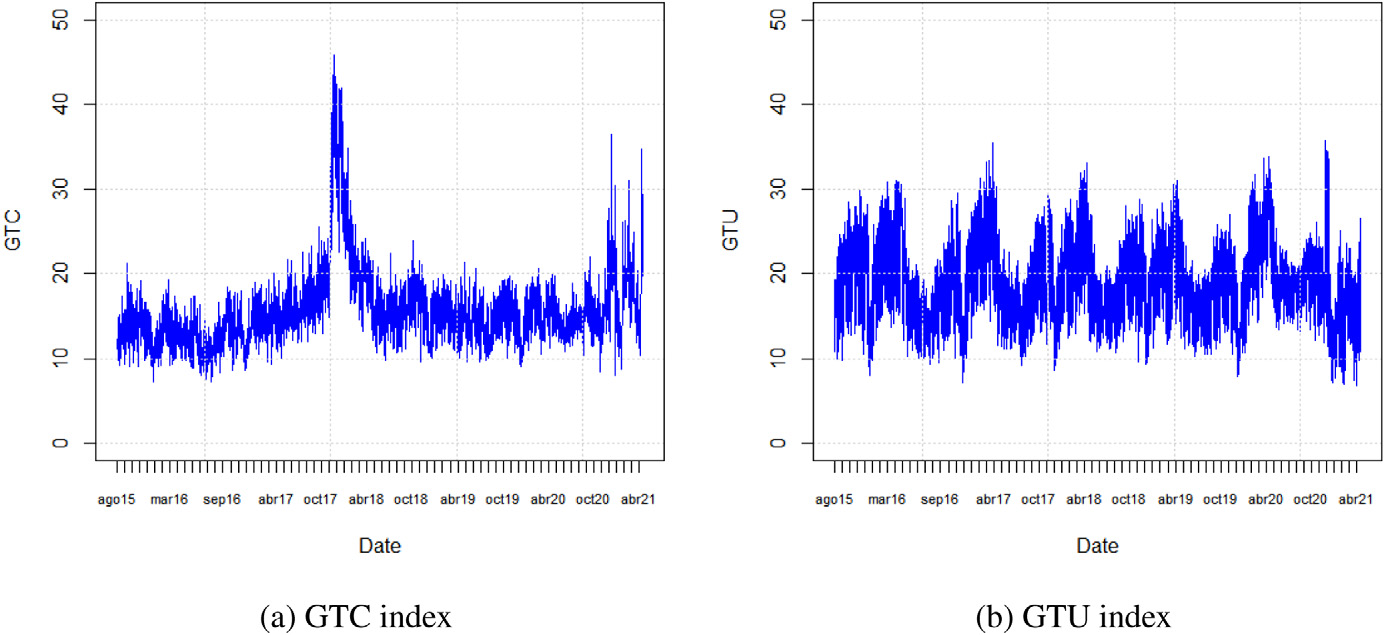
\includegraphics[width=0.9\linewidth]{gfx/m4l2_aslanidis_fig1_gtc_gtu.png}
\par\smallskip{\small \textbf{Hình 1:} Các chỉ số sự chú ý trên Google Trends: GTC và GTU (Castelnuovo and Tran, 2017).}
\end{figure}

\section{3. Phương pháp}

Chúng tôi đo lường các liên kết thông tin giữa Bitcoin và sự chú ý thị trường bằng entropy chuyển giao Shannon (transfer entropy, TE) (xem chi tiết trong Dimpfl and Peter (2013, 2018)). Entropy chuyển giao Shannon là một phương pháp phi tham số, linh hoạt, được thiết kế để khắc phục một số hạn chế của kiểm định nhân quả Granger (ví dụ như giả định tuyến tính).

Entropy chuyển giao là một thước đo dựa trên khoảng cách Kullback--Leibler của các xác suất chuyển trạng thái, cho phép không chỉ xác định hướng của luồng thông tin mà quan trọng hơn là định lượng độ mạnh của các luồng đó. Xét hai quá trình $I$ và $J$, với các phân phối xác suất biên $p(i)$ và $p(j)$, cùng phân phối xác suất đồng thời $p(i,j)$, entropy chuyển giao Shannon (TE) được định nghĩa như sau:

\begin{equation}
T_{J\to I}(k,l) = \sum_{i,j} p\left(i_{t+1}, i_t^{(k)}, j_t^{(l)}\right) \cdot \log_2\left(\frac{p\left(i_{t+1}\vert i_t^{(k)},j_t^{(l)}\right)}{p\left(i_{t+1}\vert i_t^{(k)}\right)}\right), \tag{1}
\end{equation}

trong đó $T_{J\to I}$ là thước đo lượng thông tin truyền từ $J$ đến $I$, còn $k$ và $l$ là các độ trễ (lag) được xem xét. Vì TE có thể là một ước lượng thiên lệch của lượng thông tin truyền tải, Marschinski and Kantz (2002) đề xuất một thước đo điều chỉnh, bằng cách loại bỏ phần thông tin sinh ra từ việc xáo trộn ngẫu nhiên (shuffled realization) của quá trình giải thích, như sau:

\begin{equation}
ETE_{J\to I}(k,l) = T_{J\to I}(k,l) - T_{J_{\text{shuffled}}\to I}(k,l) \tag{2}
\end{equation}

Entropy chuyển giao hiệu quả (Effective Transfer Entropy, ETE) không chỉ cho biết hướng mà còn cho biết lượng thông tin được truyền tải từ quá trình này sang quá trình kia.

Đã có tài liệu ghi nhận rằng tiền mã hóa là tài sản có độ biến động cực kỳ cao (Chaim and Laurini, 2018). Đồng thời, các lượt tìm kiếm trực tuyến có thể chịu ảnh hưởng của hành vi bầy đàn (herd behavior) (Preis et al., 2010; Bouri et al., 2019). Do đó, đáng xem xét tác động của các mức lợi suất tiền mã hóa cực đoan và các lượt tìm kiếm Google lên sự truyền tải thông tin. Ở khía cạnh này, entropy Rényi cho phép nhấn mạnh vào những phần nhất định của hàm mật độ xác suất thực nghiệm của cả hai biến.

Rényi (1970) đã phát triển một họ các thước đo thông tin thay thế cho entropy Shannon cổ điển. Một trong các thước đo đó ngày nay được biết đến với tên gọi entropy Rényi:

\begin{equation}
S_q^R(P) = \frac{1}{1-q}\log_2 \sum_{x\in X} p^q(x) \tag{3}
\end{equation}

trong đó $q$ là một tham số có thể được dùng để làm nổi bật một số phần của phân phối xác suất. Cụ thể, khi $0<q<1$, các sự kiện biên (marginal events) được nhấn mạnh nhiều hơn khi $q$ càng nhỏ trong khoảng đó. Khi $q\to 1$, ta thu lại đúng entropy Shannon.

Để ngắn gọn, chúng tôi giới thiệu độc giả tham khảo Jizba et al. (2012), Behrendt et al. (2019) để biết chi tiết về cách suy diễn entropy chuyển giao Rényi.

\section{4. Phân tích thực nghiệm}

\subsection*{4.1 Dữ liệu}

Bài báo này sử dụng dữ liệu hàng ngày về Google Trends và giá tiền mã hóa. Chúng tôi tính chỉ số Google Trends Uncertainty (GTU) của Castelnuovo and Tran (2017) cũng như chỉ số Google Trends Cryptocurrency (GTC) do chúng tôi đề xuất trong Mục 2. Dữ liệu tiền mã hóa hàng ngày được dùng để tính lợi suất logarit và độ biến động Parkinson (1980)\footnote{Mặc dù không được trình bày trong bài báo, dùng độ biến động Garman and Klass (1980) cho kết quả tương tự.}. Vì mục đích tái lập kết quả, dữ liệu sử dụng trong bài báo này được cung cấp trực tuyến cùng với bài báo. Giai đoạn khảo sát trải dài từ 07/08/2015 đến 22/04/2021, với tổng cộng 2086 quan sát.

Chúng tôi tập trung chủ yếu vào Bitcoin, vì các liên kết trên thị trường tiền mã hóa (cả về lợi suất lẫn độ biến động) đã trở nên rất mạnh trong những năm gần đây (Aslanidis et al., 2021). Như được trình bày trong tài liệu bổ sung, kết quả của chúng tôi có thể được khái quát hóa cho các đồng tiền khác như DASH, ETH, LTC và XRP.

Kết quả thực nghiệm trong mục này dùng chỉ số GTC với năm từ khóa (Tập con 3) và vẫn vững với các lựa chọn từ khóa khác. Để biết thêm chi tiết về các lựa chọn từ khóa khác nhau, xem Phụ lục A.

\subsection*{4.2 Chỉ số Google Trends Uncertainty và tiền mã hóa}

Chúng tôi khảo sát, bằng phương pháp entropy chuyển giao, sự trao đổi thông tin giữa thị trường Bitcoin và chỉ số Google Trends Uncertainty (GTU). Chúng tôi sử dụng sai phân bậc một của dữ liệu Google Trends để đảm bảo tính dừng. Bảng 1 trình bày thống kê mô tả của các biến được dùng trong phân tích.

\begin{figure}[H]
\centering
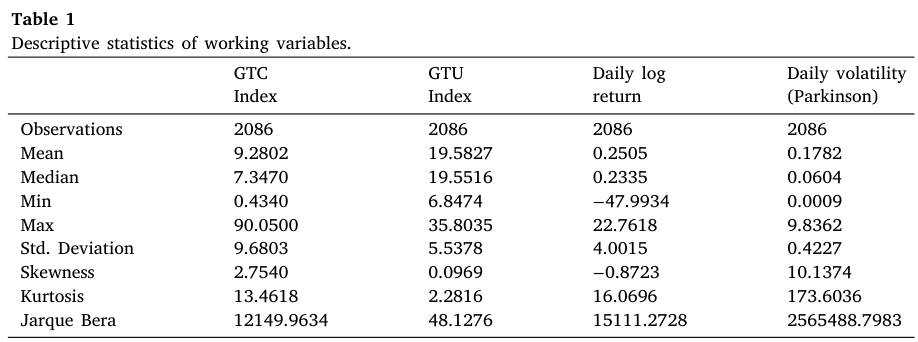
\includegraphics[width=0.8\linewidth]{gfx/m4l2_aslanidis_table1_descriptive_stats.png}
\par\smallskip{\small \textbf{Bảng 1:} Thống kê mô tả các biến được dùng trong phân tích.}
\end{figure}

Trước tiên, chúng tôi định lượng lượng thông tin truyền tải giữa GTU và Bitcoin. Bảng 2 cho thấy các luồng thông tin giữa Bitcoin và GTU không có ý nghĩa thống kê, điều này cho thấy tiền mã hóa tách biệt khỏi môi trường kinh tế vĩ mô chung. Kết quả này phù hợp với các phát hiện trước đây (Corbet et al., 2018; Aslanidis et al., 2019), vốn cho rằng các đồng tiền mã hóa lớn khá biệt lập so với các tài sản truyền thống như vàng, cổ phiếu hay trái phiếu. Phát hiện này vẫn vững đối với các lựa chọn độ trễ khác nhau, như được thể hiện trong Hình 2.

\begin{figure}[H]
\centering
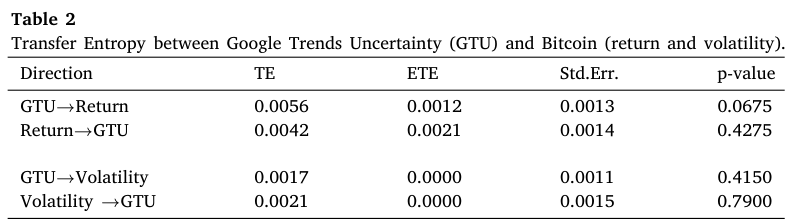
\includegraphics[width=0.8\linewidth]{gfx/m4l2_aslanidis_table2_te_gtu_bitcoin.png}
\par\smallskip{\small \textbf{Bảng 2:} Entropy chuyển giao giữa Google Trends Uncertainty (GTU) và Bitcoin (lợi suất và độ biến động).}
\end{figure}

\begin{figure}[H]
\centering
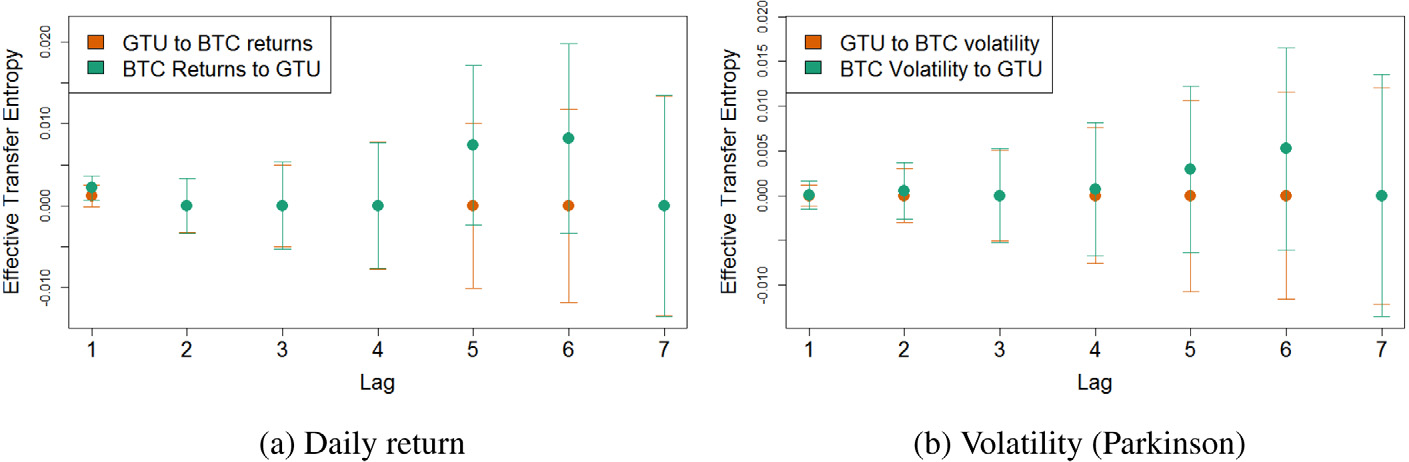
\includegraphics[width=0.9\linewidth]{gfx/m4l2_aslanidis_fig2_ete_gtu_bitcoin.png}
\par\smallskip{\small \textbf{Hình 2:} Entropy chuyển giao hiệu quả (ETE) giữa Google Trends Uncertainty (GTU) và lợi suất (a) hoặc độ biến động (b) sử dụng các độ trễ khác nhau.}
\end{figure}

\subsection*{4.3 Chỉ số Google Trends Cryptocurrency và tiền mã hóa}

Tuy nhiên, một bức tranh khác xuất hiện khi phân tích lợi suất/độ biến động của Bitcoin so với chỉ số Google Trends Cryptocurrency (GTC) được đề xuất. Bảng 3 trình bày kết quả entropy chuyển giao chỉ dùng độ trễ đầu tiên. Có thể thấy, tồn tại một luồng thông tin qua lại giữa Bitcoin và sự chú ý thị trường. Chúng tôi quan sát thấy lượng thông tin được truyền tải giữa Bitcoin và GTC là không đối xứng. Cụ thể, có nhiều thông tin rò rỉ hơn từ lợi suất (và độ biến động) của Bitcoin sang GTC so với chiều ngược lại.

\begin{figure}[H]
\centering
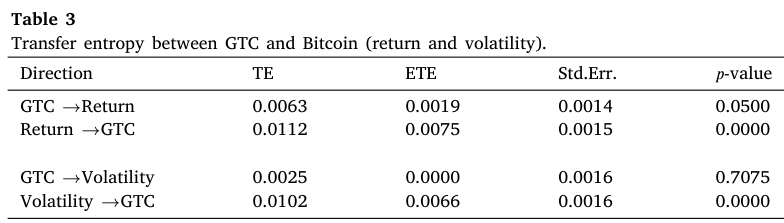
\includegraphics[width=0.8\linewidth]{gfx/m4l2_aslanidis_table3_te_gtc_bitcoin.png}
\par\smallskip{\small \textbf{Bảng 3:} Entropy chuyển giao giữa GTC và Bitcoin (lợi suất và độ biến động).}
\end{figure}

Phân tích của chúng tôi tiến thêm một bước bằng cách xem xét mối quan hệ phụ thuộc lẫn nhau, sử dụng nhiều độ trễ khác nhau của các biến. Như thể hiện trong Hình 3, lượng thông tin được truyền tải lớn hơn đối với lợi suất so với độ biến động. Hơn nữa, chúng tôi cho thấy mối quan hệ phụ thuộc lẫn nhau giữa GTC và lợi suất là hai chiều, tăng dần theo độ trễ và có ý nghĩa thống kê trong tối đa sáu ngày. Ngược lại, sự truyền tải thông tin giữa độ biến động của Bitcoin và GTC vẫn mạnh nhưng chỉ kéo dài khoảng ba đến bốn ngày, và chỉ có ý nghĩa thống kê theo chiều từ độ biến động đến GTC. Điều này hàm ý rằng tin tức được thị trường hấp thụ tương đối nhanh, mặc dù các biến động giá dường như tạo ra sự chú ý thị trường mạnh hơn trong tuần.

\begin{figure}[H]
\centering
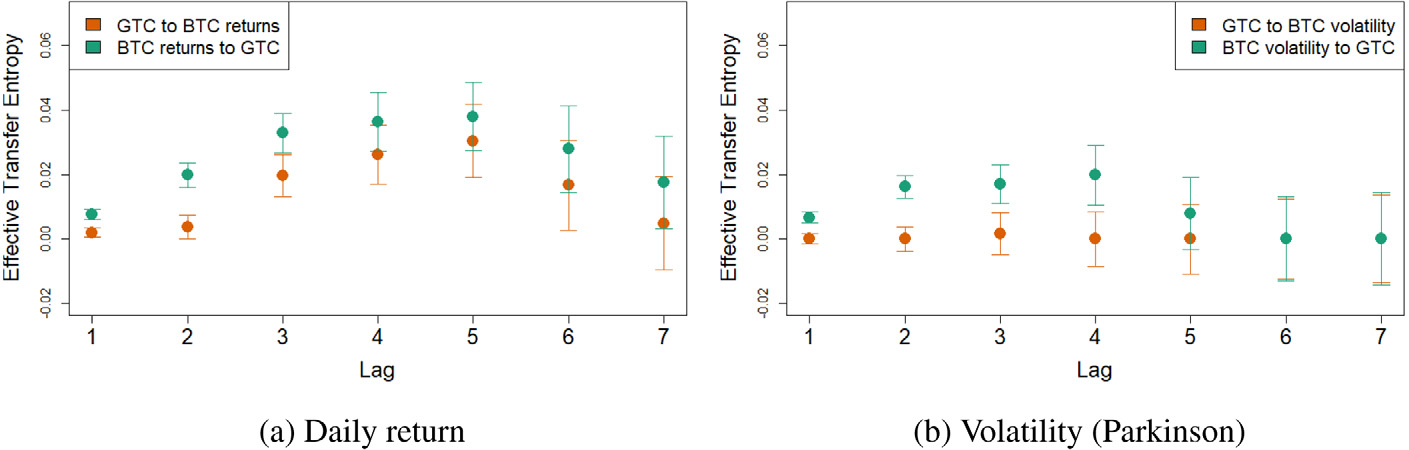
\includegraphics[width=0.9\linewidth]{gfx/m4l2_aslanidis_fig3_ete_gtc_crypto.png}
\par\smallskip{\small \textbf{Hình 3:} Entropy chuyển giao hiệu quả (ETE) giữa chỉ số Google Trends Cryptocurrency (GTC) và lợi suất (a) hoặc độ biến động (b) sử dụng các độ trễ khác nhau.}
\end{figure}

Mối liên kết hai chiều mạnh mẽ giữa Bitcoin và GTC có thể do sự chú ý ngày càng tăng của truyền thông đối với tiền mã hóa, điều khuyến khích các nhà đầu tư tìm kiếm lợi suất cao thu thập thông tin về loại tài sản tài chính mới này. Điều đó tạo ra một ``cuộc đối thoại'' giữa các lượt tìm kiếm trực tuyến và khả năng sinh lời cũng như các thước đo rủi ro của thị trường tiền mã hóa.

\subsection*{4.4 Rủi ro đuôi và truyền tải thông tin}

Entropy chuyển giao Shannon đo lường sự trao đổi thông tin giữa hai chuỗi thời gian, xem xét toàn bộ phân phối xác suất. Như đã biết, tiền mã hóa là tài sản có độ biến động rất cao và dễ xảy ra các biến động giá lớn. Đồng thời, các lượt tìm kiếm trực tuyến có thể chịu ảnh hưởng của các trào lưu nhất thời (fads), do đó thể hiện hành vi bầy đàn. Vì vậy, trong mục này chúng tôi nhằm xác định lượng thông tin nằm ở phần đuôi của phân phối lợi suất/độ biến động của Bitcoin và GTC. Entropy chuyển giao Rényi đo lường sự phụ thuộc đuôi bằng cách thiết lập giá trị của tham số $q$ trong khoảng từ 0 đến 1. Trong phân tích của mình, chúng tôi tính entropy chuyển giao Rényi cho $q=\{0.25,0.5,0.75\}$, lưu ý rằng $q$ càng nhỏ thì trọng số đặt vào phần đuôi càng lớn. Kết quả được trình bày trong Hình 4.

\begin{figure}[H]
\centering
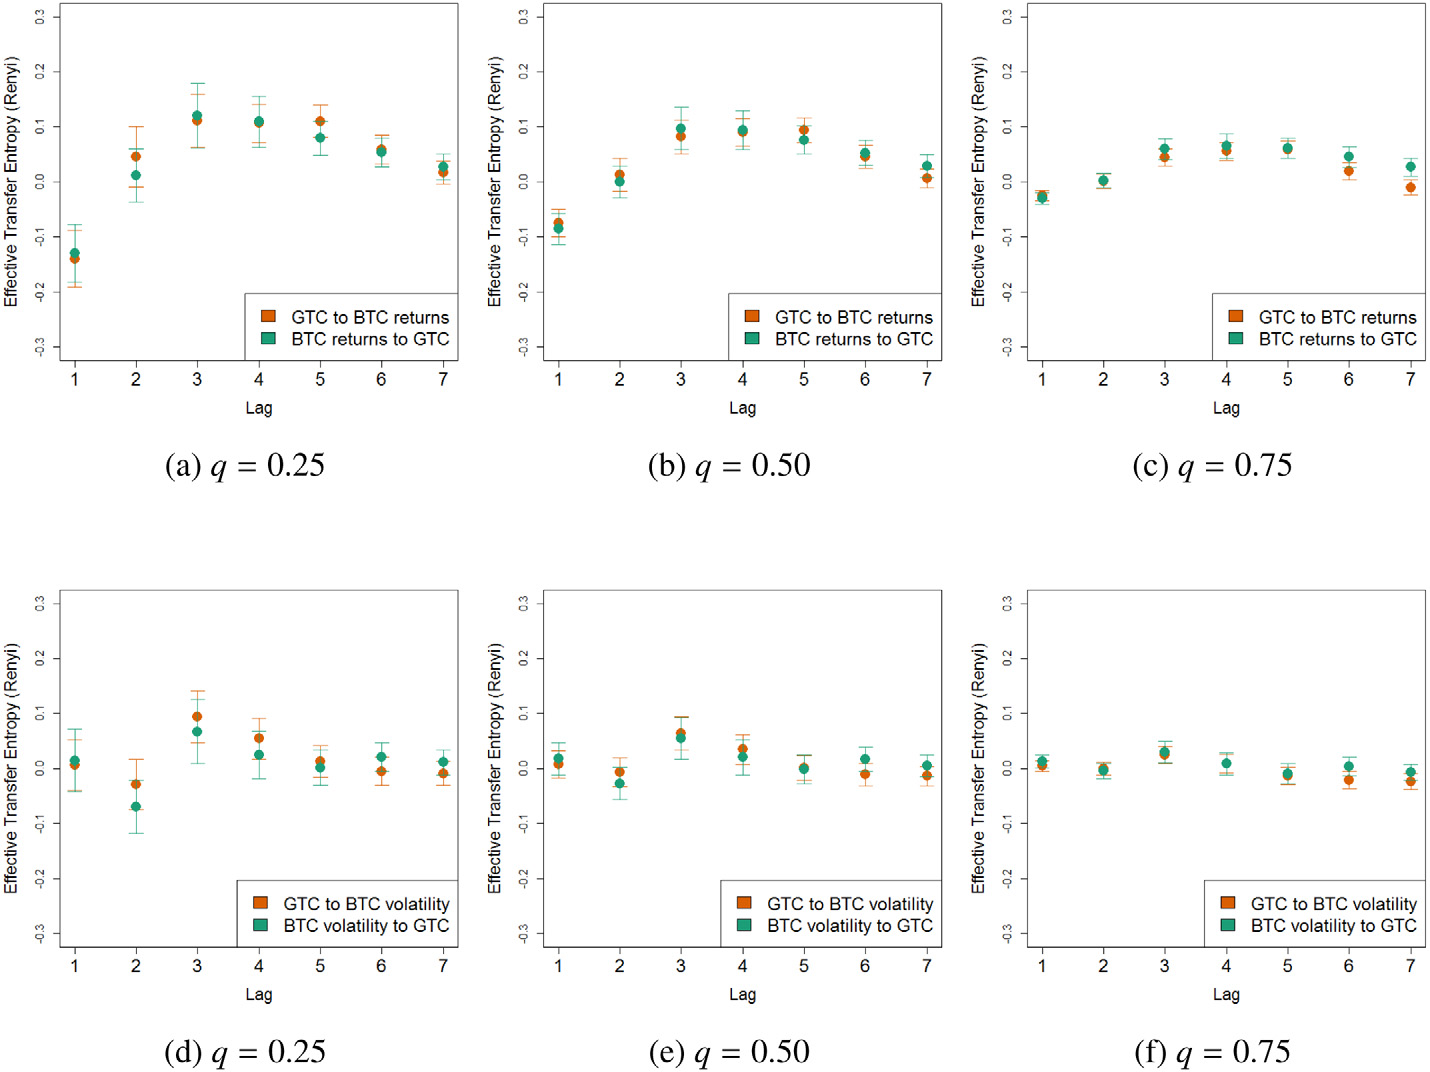
\includegraphics[width=0.95\linewidth]{gfx/m4l2_aslanidis_fig4_renyi_transfer_entropy.png}
\par\smallskip{\small \textbf{Hình 4:} Entropy chuyển giao Rényi (với các giá trị $q$ khác nhau) giữa chỉ số Google Trends Cryptocurrency (GTC) và lợi suất/độ biến động của Bitcoin (BTC) sử dụng các độ trễ khác nhau.}
\end{figure}

Phù hợp với các kết quả trước đó, luồng thông tin giữa chỉ số GTC và lợi suất Bitcoin lớn hơn so với giữa chỉ số GTC và độ biến động của Bitcoin. Tương tự, hình dạng của mối quan hệ này giữ nguyên qua các độ trễ khác nhau. Lượng thông tin truyền tải giữa GTC và lợi suất có ý nghĩa thống kê trong tối đa sáu ngày. Tuy nhiên, chúng tôi phát hiện một khác biệt đáng kể về độ lớn của luồng thông tin. Cụ thể, khi các sự kiện cực đoan được đặt trọng số cao, lượng thông tin được truyền tải lớn hơn, đạt cực đại sau ba ngày.

Đối với độ biến động, kết quả nhìn chung phù hợp với kết quả thu được khi sử dụng entropy Shannon. Sự truyền tải thông tin giữa GTC và độ biến động của Bitcoin rất ít. Tuy nhiên, khi tập trung vào các sự kiện cực đoan ($q=0.25$), vẫn có một phần thông tin được truyền tải, nhưng chỉ trong tối đa ba ngày.

\section{5. Kết luận}

Chúng tôi xác nhận rằng thị trường tiền mã hóa khá tách biệt khỏi môi trường kinh tế vĩ mô chung như được đo lường gián tiếp bằng các chỉ số Google Trends Uncertainty, chẳng hạn như chỉ số của Castelnuovo and Tran (2017). Thay vào đó, chỉ số Google Trends Cryptocurrency mà chúng tôi đề xuất truyền tải các luồng thông tin quan trọng đến (và nhận phản hồi từ) thị trường tiền mã hóa.

Chúng tôi cho thấy rằng sự truyền tải thông tin giữa Google Trends và lợi suất hàng ngày là hai chiều và kéo dài đến sáu ngày. Hơn nữa, các luồng thông tin từ độ biến động của Bitcoin đến chỉ số chú ý trên Google Trends được phát hiện là lớn hơn so với chiều ngược lại. Bài báo này cũng ghi nhận sự phụ thuộc đuôi đáng kể, cụ thể là giữa chỉ số Google Trends Cryptocurrency và lợi suất Bitcoin, phản ánh tầm quan trọng của các sự kiện cực đoan đối với những người tham gia thị trường.

Kết quả của chúng tôi vững đối với các cách kết hợp khác nhau của chỉ số Google Trends Cryptocurrency. Trên thực tế, chỉ cần năm từ khóa là đủ để nắm bắt sự chú ý thị trường, điều này phản ánh một chiến lược tìm kiếm không quá phức tạp của nhà đầu tư. Hơn nữa, các phát hiện của chúng tôi không chỉ đặc thù cho riêng Bitcoin, mà còn áp dụng được cho các đồng tiền mã hóa lớn khác như Dash, Ethereum, Litecoin và Ripple.

Gần đây, thị trường tiền mã hóa đã thu hút sự chú ý đáng kể từ các ngân hàng đầu tư (ví dụ: Morgan Stanley, Goldman Sachs), các nhà đầu tư mạo hiểm, các cơ quan quản lý (việc phê duyệt các quỹ ETF Bitcoin tại Canada) và các nhà hoạch định chính sách (quyết định của El Salvador công nhận Bitcoin và Ethereum là phương tiện thanh toán hợp pháp), cho thấy sự quan tâm của các định chế đang ngày càng gia tăng. Hơn nữa, Bank for International Settlements (2021) đã khởi động một quá trình tham vấn nhằm thu thập ý kiến về khả năng các ngân hàng thương mại nắm giữ Bitcoin và các tài sản kỹ thuật số khác. Mặc dù nghiên cứu của chúng tôi không phát hiện mối quan hệ đáng kể nào giữa Bitcoin và nền kinh tế vĩ mô nói chung, quá trình thể chế hóa tiền mã hóa có thể khiến chúng dần thâm nhập vào hệ sinh thái tài chính truyền thống. Nhìn chung, nghiên cứu của chúng tôi mang lại những hàm ý quan trọng cho việc quản lý quỹ đầu tư và hoạch định chính sách, vì nó cung cấp thông tin quan trọng để thiết kế và tái cân bằng danh mục đầu tư.

\section{Tuyên bố đóng góp tác giả (CRediT)}

\textbf{Nektarios Aslanidis:} Hình thành ý tưởng, Phương pháp luận, Viết (rà soát \& biên tập), Phân tích chính thức. \textbf{Aurelio F. Bariviera:} Hình thành ý tưởng, Phương pháp luận, Viết (rà soát \& biên tập), Phần mềm, Phân tích chính thức. \textbf{Óscar G. López:} Viết (rà soát \& biên tập), Phần mềm.

\section{Lời cảm ơn}

Nektarios Aslanidis ghi nhận sự hỗ trợ của Chính phủ Tây Ban Nha thông qua dự án PID2019-105982GB-I00. Óscar G. López ghi nhận sự hỗ trợ từ học bổng nghiên cứu của Văn phòng Quốc vụ khanh về Giáo dục và Đào tạo nghề (Secretary of State for Education and Vocational Training, Tây Ban Nha), năm 2020, mã COLAB 00559.

\section{Phụ lục A. Bộ từ khóa xây dựng Chỉ số Chú ý Google Trends Cryptocurrency (GTC)}

Xem Bảng A.4. Bảng dưới đây liệt kê các bộ từ khóa (được giữ nguyên tiếng Anh vì đây là các từ khóa tìm kiếm thực tế dùng để truy vấn Google Trends).

\textbf{Bộ đầy đủ (38 từ khóa):} AES256, altcoin, anonymity, Bitcoin, block producer, blockchain, BTC, coin, consensus, crypto, crypto crash, cryptocurrency, cryptography, digital assets, distributed ledger, ethereum, hard fork, hash, hashing, ICO, miner, minted, public key, ripple, satoshi, soft fork, stablecoin, tether, token, virtual currency, Mount Gox, Mt Gox, Mt. Gox, private key, Proof of Authority, Proof of Burn, Proof of Stake, Proof of Work.

\textbf{Tập con 1 (Subset 1):} anonymity, Bitcoin, blockchain, BTC, coin, consensus, crypto, cryptocurrency, ICO, cryptography, ethereum, hash, miner, minted, public key, ripple, satoshi, stablecoin, token, private key, Proof of Work.

\textbf{Tập con 2 (Subset 2):} Bitcoin, blockchain, BTC, crypto, cryptocurrency, cryptography, ethereum, ripple, satoshi, tether.

\textbf{Tập con 3 (Subset 3):} Bitcoin, blockchain, BTC, crypto, cryptocurrency.

\par\smallskip{\small \textbf{Bảng A.4:} Các bộ từ khóa được xem xét trong Chỉ số Chú ý Google Trends Cryptocurrency (GTC).}

\section{Phụ lục B. Dữ liệu bổ sung}

Tài liệu bổ sung liên quan đến bài báo này có thể được tìm thấy trực tuyến tại \url{https://doi.org/10.1016/j.frl.2021.102654}.

% [Đã lược bỏ danh mục Tài liệu tham khảo gốc (tiếng Anh, trích dẫn của tác giả bài gốc) để giảm dung lượng chương; không ảnh hưởng nội dung học thuật chính.]


% ---- Lesson 3 ----
% Thứ tự đọc: Lesson Notes -> Đọc thêm
\chapter{Ứng dụng của Dữ liệu Thay thế}
\label{ch:M4L3}

% Lesson: Applications of Alternative Data

\section*{Lesson Notes}

MODULE 4 | BÀI 3

\emph{Trong bài học này, chúng ta xem xét các ứng dụng của dữ liệu thay thế (alternative data). Dữ liệu thay thế trong tài chính là những nguồn dữ liệu phi truyền thống được dùng để thu được hiểu biết về xu hướng thị trường, định giá tài sản và các quyết định đầu tư. Điều này đối lập với dữ liệu truyền thống như báo cáo tài chính, hồ sơ công bố của công ty và giá thị trường. Dữ liệu văn bản từ mạng xã hội thuộc nhóm này vì nó phản ánh cảm xúc của công chúng, các bàn tán trên thị trường và sự lan truyền tin tức, những yếu tố có thể ảnh hưởng đến giá tài sản. Cụ thể, dữ liệu Twitter và StockTwits được xem là những nguồn dữ liệu thay thế có giá trị trong kỹ thuật tài chính nhờ tính thời gian thực và trọng tâm vào các thảo luận tài chính và hoạt động của thị trường chứng khoán.}

\begin{lstlisting}[language=Python,escapeinside={(*@}{@*)}]
# (*@Tải@*) (*@các@*) (*@thư@*) (*@viện@*)
import datetime
import matplotlib.pyplot as plt
import os
import pandas as pd
import plotly.express as px
import re
import requests
import zipfile

from datetime import datetime, timedelta
\end{lstlisting}

\section{Dữ liệu Twitter là gì}

Dữ liệu Twitter là lượng thông tin khổng lồ được tạo ra và chia sẻ trên nền tảng Twitter. Đây là một tập hợp thông tin đồ sộ do người dùng tạo ra trên nền tảng, bao gồm tweet, hồ sơ cá nhân, tin nhắn, xu hướng, phương tiện đa truyền thông và các tương tác. Dữ liệu này chủ yếu có sẵn ở định dạng JSON thông qua Twitter API, dù các phương pháp khác như thu thập dữ liệu web (web scraping) và công cụ của bên thứ ba cũng có thể được sử dụng. Việc truy cập dữ liệu lịch sử thường bị hạn chế, và Academic Research Track (Chương trình Nghiên cứu Học thuật) mang lại quyền truy cập rộng hơn cho các nhà nghiên cứu. Dữ liệu Twitter là nguồn tài nguyên phong phú để hiểu và phân tích thế giới trực tuyến. Dữ liệu này có giá trị đối với phân tích mạng xã hội, nghiên cứu thị trường, tình báo kinh doanh, tin tức, y tế công cộng, khoa học chính trị và nghiên cứu học thuật, cho phép thu được hiểu biết về hành vi người dùng, dư luận và các sự kiện thời gian thực.

Cấu trúc và định dạng dữ liệu:

\begin{itemize}
  \item JSON: Twitter API chủ yếu cung cấp dữ liệu ở định dạng JSON (JavaScript Object Notation). JSON là một định dạng trao đổi dữ liệu gọn nhẹ, dễ đọc và dễ viết đối với con người, đồng thời dễ phân tích cú pháp và tạo ra đối với máy. Mỗi tweet, hồ sơ người dùng hoặc đối tượng dữ liệu khác được biểu diễn như một đối tượng JSON với nhiều thuộc tính và giá trị.
  \item CSV/TSV: Dữ liệu Twitter cũng có thể được xuất hoặc chuyển đổi sang định dạng CSV (Comma-Separated Values) hoặc TSV (Tab-Separated Values) để phân tích trong phần mềm bảng tính hoặc các công cụ khác.
  \item Cơ sở dữ liệu: Đối với phân tích và lưu trữ quy mô lớn, dữ liệu Twitter thường được nạp vào các cơ sở dữ liệu như MySQL, PostgreSQL hoặc các cơ sở dữ liệu NoSQL như MongoDB.
\end{itemize}

Truy cập dữ liệu Twitter và các hạn chế:

\begin{itemize}
  \item Twitter API: Dù Twitter API là cách truy cập dữ liệu mạnh mẽ, vẫn có những giới hạn và hạn chế. Chúng bao gồm giới hạn tần suất (rate limit) về số yêu cầu có thể gửi, chỉ truy cập được một phần dữ liệu lịch sử (thường là 7 ngày gần nhất đối với API tiêu chuẩn), và yêu cầu về tài khoản nhà phát triển cùng khóa API.
  \item Academic Research Track: Đối với các nhà nghiên cứu học thuật, Twitter cung cấp ``Academic Research Track'' với mức truy cập nâng cao và lượng dữ liệu sẵn có lớn hơn. Chương trình này đòi hỏi một đề xuất nghiên cứu chi tiết và quy trình phê duyệt.
  \item Thiên lệch dữ liệu và các cân nhắc đạo đức: Cần lưu ý những thiên lệch tiềm ẩn trong dữ liệu Twitter, chẳng hạn việc một số nhóm nhân khẩu học hoặc quan điểm được đại diện quá mức. Các cân nhắc đạo đức là thiết yếu, bao gồm tôn trọng quyền riêng tư của người dùng, xin sự đồng ý có hiểu biết khi cần thiết và tránh lan truyền thông tin sai lệch. Dữ liệu Twitter vốn thiên về những người dùng tích cực và các ý kiến được chia sẻ công khai. Tập dữ liệu này có thể không đại diện cho quan điểm của toàn bộ cộng đồng nhà đầu tư.
  \item Tính thưa thớt và chất lượng dữ liệu: Tập dữ liệu có thể chứa những khoảng trống hoặc những giai đoạn có khối lượng tweet thấp, điều này có thể ảnh hưởng đến phân tích. Điều thiết yếu là kiểm tra chất lượng dữ liệu và xử lý mọi vấn đề tiềm ẩn như giá trị thiếu hoặc sự không nhất quán trước khi tiến hành phân tích.
\end{itemize}

Có nhiều lựa chọn để tải các tập dữ liệu Twitter có sẵn, với nhiều con đường phục vụ cả nhà nghiên cứu lẫn người dùng thông thường, với các mức truy cập và đặc thù dữ liệu khác nhau:

\begin{itemize}
  \item Dành cho nhà nghiên cứu: Twitter Academic Research Track cung cấp quyền truy cập toàn diện nhất, nhưng đòi hỏi nộp đơn và được phê duyệt.
  \item Các lựa chọn công khai: Các nền tảng như Kaggle, figshare, Zenodo, Data.World, Hugging Face, IEEE DataPort và Mendeley Data lưu trữ nhiều tập dữ liệu về các chủ đề khác nhau, sẵn sàng để tải xuống. Kaggle là nền tảng do cộng đồng vận hành nổi bật nhất trong số được nêu. IEEE DataPort tập trung hơn vào việc chia sẻ dữ liệu nghiên cứu trong các lĩnh vực cụ thể. Hugging Face là nền tảng do cộng đồng dẫn dắt, chuyên về NLP và các lĩnh vực liên quan.
  \item Các nguồn chuyên biệt: Các cơ quan chính phủ và tổ chức có thể cung cấp các tập dữ liệu liên quan đến những sự kiện hoặc chủ đề cụ thể.
\end{itemize}

Khi sử dụng các nền tảng này, có lẽ điều quan trọng nhất là tuân thủ các thực hành dữ liệu có trách nhiệm và ưu tiên tính hợp pháp, sự bảo vệ người dùng và ứng xử có đạo đức, nhằm bảo đảm niềm tin và tác động xã hội tích cực. Cấp phép dữ liệu, quyền riêng tư của người dùng và các cân nhắc đạo đức là thiết yếu cho việc sử dụng dữ liệu có trách nhiệm. Việc cấp phép bảo đảm tuân thủ pháp lý, quyền riêng tư bảo vệ thông tin cá nhân, và đạo đức định hướng các thực hành dữ liệu công bằng và tôn trọng. Những khía cạnh này cũng có vai trò then chốt đối với dữ liệu công khai, đòi hỏi tuân thủ các điều khoản giấy phép, ẩn danh hóa để bảo vệ quyền riêng tư và ý thức về những thiên lệch tiềm ẩn để phân tích có đạo đức.

\subsection{Lấy dữ liệu Twitter}

Trong bài học này, chúng ta khám phá dữ liệu Stock Market Tweets từ IEEE Dataport, có tại \url{https://dx.doi.org/10.21227/g8vy-5w61}. IEEE DataPort là một kho lưu trữ được tuyển chọn dành cho dữ liệu nghiên cứu, chủ yếu tập trung vào các lĩnh vực kỹ thuật và công nghệ. Kho này do Viện Kỹ sư Điện và Điện tử (Institute of Electrical and Electronics Engineers, IEEE) vận hành và khuyến khích các nhà nghiên cứu chia sẻ tập dữ liệu của mình để thúc đẩy tri thức trong lĩnh vực tương ứng. Tập dữ liệu này chứa một bộ sưu tập các tweet liên quan đến thị trường chứng khoán, đặc biệt tập trung vào chỉ số S\&P 500. Mục tiêu là cung cấp dữ liệu cho các nhà nghiên cứu và người thực hành quan tâm đến việc phân tích mối quan hệ giữa cảm xúc trên mạng xã hội và biến động của thị trường chứng khoán.

Tập dữ liệu này được cung cấp theo giấy phép Creative Commons Attribution 4.0 International (CC BY 4.0). Giấy phép này cho phép sử dụng, chia sẻ, chỉnh sửa và phân phối lại dữ liệu một cách tự do, miễn là ghi công phù hợp cho những người tạo ra bản gốc.

Tập dữ liệu bao phủ các tweet từ ngày 9 tháng 4 năm 2020 đến ngày 16 tháng 7 năm 2020. Khoảng thời gian này cung cấp lượng dữ liệu đáng kể cho phân tích và bao quát nhiều điều kiện thị trường khác nhau. Dữ liệu được thu thập bằng thẻ S\&P 500 (\#SPX500), các đề cập đến 25 công ty hàng đầu trong chỉ số S\&P 500, và thẻ Bloomberg (\#stocks). Dữ liệu được đóng gói trong một tệp lưu trữ ZIP gồm hai tệp CSV: tệp 'tweets\_labelled\_09042020\_16072020.csv' gồm 5.000 tweet được chọn bằng lấy mẫu ngẫu nhiên. Trong số 5.000 tweet đó, 1.300 tweet được gán nhãn thủ công vào các lớp tích cực, trung lập hoặc tiêu cực. Tệp thứ hai 'tweets\_remaining\_09042020\_16072020.csv' chứa phần còn lại của các tweet.

Đoạn mã dưới đây được thiết kế để giải nén một tệp ZIP chứa dữ liệu Twitter, rồi định vị tất cả các tệp CSV trong thư mục đã giải nén để xử lý tiếp. Mã lặp qua danh sách các tệp CSV chứa dữ liệu Twitter, đọc từng tệp vào một DataFrame pandas, chuẩn hóa tên cột chứa văn bản tweet, rồi gộp tất cả các DataFrame thành một DataFrame duy nhất có tên \texttt{twitter\_df}:

\begin{lstlisting}[language=Python,escapeinside={(*@}{@*)}]
# (*@Giải@*) (*@nén@*) (*@tệp@*) ZIP (*@vào@*) (*@thư@*) (*@mục@*) (*@có@*) (*@tên@*) 'extracted_tweets'
with zipfile.ZipFile('tweets.zip', 'r') as zip_ref:
    zip_ref.extractall('extracted_tweets')

# (*@Lấy@*) danh (*@sách@*) (*@các@*) (*@tệp@*) CSV trong (*@thư@*) (*@mục@*) 'tweets' (*@bên@*) trong
tweets_folder = 'extracted_tweets/tweets'
csv_files = [f for f in os.listdir(tweets_folder) if f.endswith('.csv')]

# (*@Lặp@*) qua (*@các@*) (*@tệp@*) CSV (*@và@*) (*@đọc@*) (*@chúng@*) (*@vào@*) (*@các@*) DataFrame
dfs = []
for csv_file in csv_files:
    file_path = os.path.join(tweets_folder, csv_file)
    df = pd.read_csv(file_path, sep=';')

    # (*@Đổi@*) (*@tên@*) (*@cột@*) 'full_text' (*@hoặc@*) 'text' (*@thành@*) (*@tên@*) chung 'tweet_text'
    if 'full_text' in df.columns:
        df = df.rename(columns={'full_text': 'tweet_text'})
    elif 'text' in df.columns:
        df = df.rename(columns={'text': 'tweet_text'})

    dfs.append(df)

# (*@Nối@*) (*@tất@*) (*@cả@*) (*@các@*) DataFrame (*@thành@*) (*@một@*) DataFrame duy (*@nhất@*) (*@và@*) (*@hiển@*) (*@thị@*) (*@nó@*)
twitter_df = pd.concat(dfs, ignore_index=True)
twitter_df
\end{lstlisting}

\begin{lstlisting}[escapeinside={(*@}{@*)}]
BadZipFile
\end{lstlisting}

\subsection{Điều chỉnh múi giờ trong dữ liệu Twitter}

Bây giờ hãy quan sát định dạng ngày và giờ trong cột 'created\_at'. Ký hiệu ``+00:00'' trong các giá trị của 'created\_at' chỉ một múi giờ. Nó biểu diễn độ lệch so với Giờ Phối hợp Quốc tế (UTC), trong trường hợp này là 0 giờ. Điều này có nghĩa là các dấu thời gian đang ở chính UTC. Hãy chuyển đổi chúng sang múi giờ New York. Ta thực hiện bằng hàm \texttt{pd.to\_datetime()}, hàm này chuyển cột 'created\_at' thành các đối tượng DateTime của pandas. Sau đó ta áp dụng chuỗi hàm \texttt{.dt.tz\_convert('America/New\_York')}, hàm này chuyển các đối tượng DateTime sang múi giờ New York bằng tên múi giờ IANA 'America/New\_York'. Điều này bảo đảm các dấu thời gian được điều chỉnh theo các lần chuyển đổi giờ mùa hè tại New York:

\begin{lstlisting}[language=Python,escapeinside={(*@}{@*)}]
# (*@Chuyển@*) (*@các@*) (*@dấu@*) (*@thời@*) gian sang (*@múi@*) (*@giờ@*) New York
twitter_df['created_at'] = pd.to_datetime(twitter_df['created_at']).dt.tz_convert('America/New_York')
twitter_df
\end{lstlisting}

\begin{lstlisting}[escapeinside={(*@}{@*)}]
NameError
\end{lstlisting}

\subsection{Phát hiện retweet trong dữ liệu Twitter}

Trên Twitter, ``RT'' là chữ viết tắt phổ biến của ``retweet''. Khi một người dùng muốn chia sẻ tweet của người khác với những người theo dõi của mình, họ có thể retweet. ``RT'' là dấu hiệu then chốt của các retweet trên Twitter. Nó được dùng trong các retweet thủ công, retweet có trích dẫn, và là một quy ước đã trở thành một phần của văn hóa Twitter. Bằng cách tìm kiếm ``RT'' ở đầu các tweet, chúng ta có thể nhận diện retweet một cách hiệu quả trong phân tích dữ liệu.

Bây giờ hãy lấy bộ sưu tập tweet của chúng ta và tách chúng thành hai nhóm: một nhóm cho retweet và một nhóm cho tweet gốc (hoặc các loại tweet khác không phải retweet). Đoạn mã dưới đây lấy DataFrame \texttt{twitter\_df} chứa dữ liệu Twitter và tách nó thành hai DataFrame mới bằng cách lọc cột 'tweet\_text'. Sau đó mã hiển thị cả \texttt{retweets\_df} và \texttt{remainder\_df} bằng hàm \texttt{display()}:

\begin{lstlisting}[language=Python,escapeinside={(*@}{@*)}]
# (*@Tạo@*) (*@một@*) DataFrame (*@chỉ@*) (*@chứa@*) (*@các@*) retweet
retweets_df = twitter_df[twitter_df['tweet_text'].str.startswith('RT')]

# (*@Tạo@*) (*@một@*) DataFrame (*@chứa@*) (*@các@*) tweet (*@không@*) (*@phải@*) retweet
remainder_df = twitter_df[~twitter_df['tweet_text'].str.startswith('RT')]

# (*@Hiển@*) (*@thị@*) (*@các@*) DataFrame
print("## Retweets DataFrame:")
print("This DataFrame contains only retweets from the Twitter data.")
display(retweets_df)

print("\n## Remainder DataFrame:")
print("This DataFrame contains tweets that are not retweets.")
display(remainder_df)
\end{lstlisting}

\begin{lstlisting}[escapeinside={(*@}{@*)}]
NameError
\end{lstlisting}

Ở đây ta thấy \texttt{retweets\_df} có 350.752 hàng và \texttt{remainder\_df} có 577.921 hàng. Cần lưu ý rằng các DataFrame được tách dựa trên việc một tweet có phải là retweet hay không. Số hàng của \texttt{retweets\_df} và \texttt{remainder\_df} cho ta ý niệm về tỷ lệ retweet trong tập dữ liệu, nhưng điều này không cho biết trực tiếp có bao nhiêu tweet gốc riêng biệt đã được retweet. Một tweet gốc có thể được nhiều người dùng khác nhau retweet nhiều lần, vì vậy 350.752 hàng trong \texttt{retweets\_df} có thể đại diện cho một số lượng tweet gốc riêng biệt nhỏ hơn nhiều đã được retweet nhiều lần. Chúng ta cũng nên xét đến hiệu ứng độ trễ thời gian dựa trên hành vi Twitter điển hình. Rất có khả năng phần lớn các retweet trong tập dữ liệu của chúng ta thuộc cùng giai đoạn, nhưng một số retweet sẽ đến từ giai đoạn sớm hơn đôi chút so với các tweet gốc mà chúng ta đã thu thập.

\subsection{Tìm hiểu phân phối của các tweet}

Bây giờ hãy thử tìm hiểu phân phối của các tweet theo thời gian. Đoạn mã dưới đây lấy cột 'created\_at' làm chỉ mục để lấy mẫu lại (resampling). Sau đó nó lấy mẫu lại dữ liệu theo tuần và tính số lượng tweet trong mỗi khoảng tuần. Cuối cùng, nó đếm số tweet xảy ra trong mỗi tuần:

\begin{lstlisting}[language=Python,escapeinside={(*@}{@*)}]
# (*@Lấy@*) (*@số@*) (*@lượng@*) tweet theo (*@tuần@*)
weekly_counts = twitter_df.set_index('created_at').resample('W-MON', label='left', closed='left').count()
weekly_counts = weekly_counts.rename_axis(index="Week Starting")
display(weekly_counts)
\end{lstlisting}

\begin{lstlisting}[escapeinside={(*@}{@*)}]
NameError
\end{lstlisting}

Ở đây \texttt{.resample('W-MON', label='left', closed='left')} là phần cốt lõi của thao tác. \texttt{.resample('W-MON')} lấy mẫu lại dữ liệu vào các khoảng theo tuần, bắt đầu từ thứ Hai ('W-MON'). \texttt{label='left'} chỉ ra rằng nhãn của mỗi khoảng phải là mép trái (điểm bắt đầu) của khoảng. \texttt{closed='left'} quy định mép trái của mỗi khoảng là đóng (được bao gồm trong khoảng). Điều này có nghĩa là các tweet được tạo vào thứ Hai sẽ được tính vào khoảng của tuần đó.

Bảng phân phối theo tuần này tạo cơ hội quan sát các xu hướng hoạt động tweet theo thời gian. Ở đây ta thấy số lượng tweet nhìn chung dao động nhưng có vẻ tương đối cao trong suốt tháng Sáu và tháng Bảy. Và có hai tuần (11 tháng 5 và 18 tháng 5) không ghi nhận tweet nào, và có thể cả tuần kế tiếp (25 tháng 5) cũng có hoạt động tweet giảm. Điều này có thể cho thấy một vấn đề trong thu thập dữ liệu hoặc một giai đoạn hoạt động thấp.

\subsection{Trực quan hóa dữ liệu Twitter}

Bằng cách xem xét khối lượng dữ liệu và áp dụng các kỹ thuật trực quan hóa phù hợp, chúng ta có thể thu được những hiểu biết có ý nghĩa hơn từ biểu đồ số lượng tweet hàng ngày. Bây giờ hãy nhóm dữ liệu theo ngày và vẽ số lượng tweet hàng ngày cho DataFrame \texttt{twitter\_df} để khảo sát. Đoạn mã dưới đây trước hết nhóm DataFrame \texttt{twitter\_df} theo phần ngày của cột 'created\_at' bằng \texttt{dt.date} để trích xuất ngày. Việc này tạo ra các nhóm tweet cho mỗi ngày. Sau đó nó đếm số tweet trong mỗi nhóm bằng \texttt{['tweet\_text'].count()}, hàm đếm các giá trị không rỗng trong cột 'tweet\_text'. Tiếp theo chúng ta vẽ dữ liệu:

\begin{lstlisting}[language=Python,escapeinside={(*@}{@*)}]
# (*@Nhóm@*) theo (*@ngày@*) (*@và@*) (*@đếm@*)
daily_tweet_counts_twitter_all = twitter_df.groupby(twitter_df['created_at'].dt.date)['tweet_text'].count()

# (*@Vẽ@*) (*@biểu@*) (*@đồ@*)
plt.figure(figsize=(12, 6))

plt.plot(daily_tweet_counts_twitter_all.index, daily_tweet_counts_twitter_all.values, label='Twitter (All Data)', marker='o')

plt.xlabel('Date')
plt.ylabel('Number of Tweets')
plt.title('Daily Tweet Counts - Twitter (All Data)')
plt.legend()
plt.grid(True)

plt.xticks(rotation=45, ha='right')  # Xoay (*@nhãn@*) (*@trục@*) x (*@để@*) (*@dễ@*) (*@đọc@*) (*@hơn@*)

plt.tight_layout()  # (*@Điều@*) (*@chỉnh@*) (*@bố@*) (*@cục@*) (*@để@*) (*@tránh@*) (*@nhãn@*) (*@chồng@*) (*@lên@*) nhau
plt.show()
\end{lstlisting}

\begin{lstlisting}[escapeinside={(*@}{@*)}]
NameError
\end{lstlisting}

Bằng cách xem xét biểu đồ, chúng ta có thể nhận diện mọi khoảng trống hoặc giai đoạn có số lượng tweet thấp hơn đáng kể hoặc bằng không. Những khoảng trống này có thể cho thấy dữ liệu bị thiếu hoặc những giai đoạn hoạt động tweet suy giảm. Nếu cần khảo sát sâu hơn các khoảng trống hoặc mẫu hình cụ thể, chúng ta có thể điều chỉnh khoảng thời gian của biểu đồ hoặc thêm chú thích để làm nổi bật các vùng đáng quan tâm. Trong trường hợp của chúng ta, ta biết rằng có một khoảng trống trong giai đoạn từ ngày 10 tháng 5 đến ngày 27 tháng 5 năm 2020. Điều này có nghĩa là hoặc không có tweet nào được thu thập hay ghi nhận trong giai đoạn đó, hoặc chúng đã bị lọc bỏ trong quá trình xử lý dữ liệu.

Có nhiều kỹ thuật điền khuyết dữ liệu (data imputation) để lấp đầy dữ liệu bị thiếu. Với cách tiếp cận đơn giản, chúng ta có thể lấp khoảng trống bằng số lượng tweet trung bình của những ngày trước và sau khoảng trống. Với những tình huống phức tạp hơn, chúng ta có thể khám phá các kỹ thuật điền khuyết chuỗi thời gian hoặc các mô hình học máy để dự đoán các giá trị bị thiếu dựa trên các mẫu hình trong dữ liệu hiện có. Tuy nhiên, việc này cần được thực hiện thận trọng và có ý thức về những thiên lệch tiềm ẩn do điền khuyết đưa vào. Trong trường hợp của chúng ta, không kỹ thuật nào trong số này có thể chính xác, vì có một khoảng trống đáng kể mà trong đó các xu hướng hoặc sự kiện có thể rất khó lường để suy ra hay mô hình hóa. Do đó, chúng ta tạm giữ nguyên khoảng trống này và tiếp tục các khám phá sâu hơn.

\subsection{Phát hiện cashtag và hashtag trong dữ liệu Twitter}

Trong các tweet Twitter, mã cổ phiếu có thể xuất hiện dưới dạng cashtag (ví dụ \$AAPL, \$GOOG) hoặc hashtag (ví dụ \#AAPL, \#GOOG), cả hai thường đại diện cho mã chứng khoán (ticker) của một công ty. Cashtag ngày càng phổ biến, nhưng hashtag vẫn được dùng cho các thảo luận hoặc sự kiện liên quan đến cổ phiếu ở phạm vi rộng hơn. Các ký hiệu này có thể được đặt ở bất kỳ vị trí nào trong một tweet và thường cung cấp ngữ cảnh cho thông điệp, gắn nó với một cổ phiếu hoặc chủ đề cụ thể.

Bây giờ hãy khám phá vài hiểu biết về việc những cổ phiếu nào được thảo luận thường xuyên nhất trong dữ liệu Twitter của chúng ta. Đoạn mã dưới đây trước hết trích xuất các mã cổ phiếu từ phần đầu của mỗi tweet trong DataFrame \texttt{twitter\_df} bằng biểu thức chính quy (regular expression) và lưu chúng vào một cột mới 'stock\_symbols'. Sau đó, nó ``bung'' (explode) cột này để tạo các hàng riêng cho mỗi mã trong một tweet. Nó chuyển các mã sang chữ thường, đếm số lần xuất hiện, sắp xếp theo tần suất giảm dần, và cuối cùng hiển thị 10 mã cổ phiếu được đề cập thường xuyên nhất trong tập dữ liệu:

\begin{lstlisting}[language=Python,escapeinside={(*@}{@*)}]
# (*@Phát@*) (*@hiện@*) (*@mã@*) (*@cổ@*) (*@phiếu@*) (*@và@*) hashtag
twitter_df['cashtags_hashtags'] = twitter_df['tweet_text'].str.findall(r'(?:\$|#)([a-zA-Z]+\.*[a-zA-Z]+)')
twitter_df.explode('cashtags_hashtags')['cashtags_hashtags'].str.lower().value_counts().sort_values(ascending=False).head(10)
\end{lstlisting}

\begin{lstlisting}[escapeinside={(*@}{@*)}]
cashtags_hashtags
stocks         262381
spx            190857
aapl           123629
spy            115031
amzn           108484
fb              85685
es              66068
stockmarket     65091
msft            62018
trading         60261
Name: count, dtype: int64
\end{lstlisting}

Ở đây \texttt{.str.findall(r'(?:\textbackslash{}\$|\#)([a-zA-Z]+\textbackslash{}.*[a-zA-Z]+)')} áp dụng một biểu thức chính quy để tìm và trích xuất cashtag và hashtag từ văn bản tweet. Hãy phân tích biểu thức chính quy này:

\begin{itemize}
  \item \texttt{(?: ... )}: Tạo một nhóm không bắt (non-capturing group). Điều này có nghĩa là phần này của biểu thức chính quy được dùng để khớp, nhưng nội dung khớp sẽ không được bắt và lưu riêng.
  \item \texttt{\textbackslash{}\$|\#}: Khớp với một dấu đô la nguyên văn (\$) hoặc một dấu thăng hashtag (\#). Ký hiệu \texttt{ | } biểu diễn điều kiện ``hoặc''.
  \item \texttt{[a-zA-Z]+}: Khớp với một hoặc nhiều chữ cái (a-z, A-Z).
  \item \texttt{\textbackslash{}.*}: Khớp với không hoặc một dấu chấm (.), cho phép các mã có dấu chấm (ví dụ \$BRK.B).
  \item \texttt{[a-zA-Z]+}: Lại khớp với một hoặc nhiều chữ cái, bắt phần còn lại của mã sau dấu chấm (nếu có).
\end{itemize}

Như vậy, toàn bộ biểu thức chính quy ở dòng đầu tiên trong đoạn mã trên tìm các mẫu trông giống cashtag của mã cổ phiếu (ví dụ \$AAPL, \$AAPL, \$GOOG, \$BRK.B) hoặc hashtag và lưu chúng vào một cột mới có tên 'cashtags\_hashtags'.

\texttt{twitter\_df.explode('cashtags\_hashtags')} ở dòng thứ hai của đoạn mã trên ``bung'' cột 'cashtags\_hashtags', biến mỗi danh sách cashtag/hashtag thành các hàng riêng. Vì vậy, nếu một tweet có nhiều cashtag/hashtag, giờ nó sẽ có nhiều hàng, mỗi hàng một thẻ. Sau đó phần còn lại của dòng thứ hai trong đoạn mã trên lấy các cashtag/hashtag đã trích xuất, đếm số lần mỗi thẻ xuất hiện trong các tweet, sắp xếp theo tần suất và hiển thị 10 cashtag/hashtag được đề cập nhiều nhất.

Nhìn chung, bảng này nhấn mạnh rằng chỉ số S\&P 500 (spx) cùng với SPDR S\&P 500 ETF Trust (spy) và hợp đồng tương lai E-mini S\&P 500 (es) (cả hai đều là các công cụ tài chính theo dõi hiệu suất của chỉ số S\&P 500) nằm trong số 10 đề cập hàng đầu của tập dữ liệu Twitter này. Điều này không đáng ngạc nhiên vì bản thân tập dữ liệu Twitter này ban đầu được thu thập bằng thẻ S\&P 500 và các thẻ của 25 công ty hàng đầu trong chỉ số S\&P 500. Từ bảng trên, ta cũng có thể thấy rằng các công cụ tài chính khác được thảo luận nhiều nhất trong dữ liệu Twitter đã phân tích là Apple (aapl), Amazon (amzn), FB (fb) và Microsoft (msft). Các hashtag ``stocks'', ``stockmarket'' và ``trading'' càng nhấn mạnh trọng tâm của tập dữ liệu vào các chủ đề liên quan đến thị trường chứng khoán. Thông tin này có thể có giá trị để hiểu các xu hướng thị trường, cảm xúc nhà đầu tư và trọng tâm chung của các thảo luận tài chính trên Twitter trong giai đoạn mà tập dữ liệu bao phủ.

\subsection{Lọc dữ liệu Twitter}

Bây giờ hãy thử lọc một số tweet theo các thuật ngữ cụ thể. Đoạn mã dưới đây định nghĩa một hàm có tên \texttt{contains\_spy()} kiểm tra xem một chuỗi văn bản cho trước có chứa bất kỳ đề cập nào đến SPY ETF (SPDR S\&P 500 ETF Trust) hay không, có xét đến các biến thể văn bản khác nhau. Lần này chúng ta kiểm tra toàn bộ văn bản tweet thay vì chỉ tìm cashtag và hashtag. Trước hết ta dùng \texttt{text.lower()} để chuyển văn bản đầu vào sang chữ thường nhằm bảo đảm khớp không phân biệt hoa thường. \texttt{patterns = [...]} định nghĩa một danh sách các mẫu biểu thức chính quy biểu diễn những cách khác nhau mà SPY ETF có thể được đề cập. Nó bao gồm các biến thể như ``spy'', ``\$spy'', ``\#spy'', ``spydr'', ``s\&p 500 etf'', có và không có ranh giới từ (\textbackslash b). Ranh giới từ bảo đảm rằng ``spy'' không bị khớp bên trong các từ như ``spying''. Về bản chất, hàm này nhằm nhận diện các mục văn bản trong tweet có đề cập đến SPY ETF, bất kể nó được viết như thế nào. Sau đó mã lọc DataFrame \texttt{twitter\_df} để chỉ giữ lại các tweet đề cập đến SPY ETF, bằng hàm \texttt{contains\_spy()}:

\begin{lstlisting}[language=Python,escapeinside={(*@}{@*)}]
# (*@Định@*) (*@nghĩa@*) (*@một@*) (*@hàm@*) (*@kiểm@*) tra (*@các@*) (*@đề@*) (*@cập@*) (*@đến@*) S&P 500 (*@kèm@*) (*@các@*) (*@biến@*) (*@thể@*)
def contains_spy(text):
    # (*@Xử@*) (*@lý@*) (*@các@*) (*@biến@*) (*@thể@*) (*@về@*) (*@khoảng@*) (*@trắng@*), "&" (*@và@*) (*@chữ@*) (*@hoa/thường@*)
    text = text.lower()  # (*@Chuyển@*) sang (*@chữ@*) (*@thường@*) (*@để@*) (*@khớp@*) (*@không@*) (*@phân@*) (*@biệt@*) hoa (*@thường@*)
    text = re.sub(r"[^a-zA-Z0-9 ]", "", text)  # (*@Loại@*) (*@bỏ@*) (*@các@*) (*@ký@*) (*@tự@*) (*@đặc@*) (*@biệt@*) (*@ngoại@*) (*@trừ@*) (*@khoảng@*) (*@trắng@*)

    # (*@Kiểm@*) tra (*@các@*) (*@mẫu@*) (*@khác@*) nhau
    patterns = [
        r"\bspy\b",  # (*@Dùng@*) ranh (*@giới@*) (*@từ@*) (\b) (*@để@*) (*@tránh@*) (*@bắt@*) (*@một@*) (*@phần@*) (*@của@*) (*@từ@*) ((*@ví@*) (*@dụ@*) "spying")
        r"\$spy",  # Cashtag
        r"#spy",  # Hashtag
        r"\b\$spy\b",  # Cashtag (*@kèm@*) ranh (*@giới@*) (*@từ@*)
        r"\b#spy\b",  # Hashtag (*@kèm@*) ranh (*@giới@*) (*@từ@*)
        r"\bspdr\b",  # (*@Một@*) (*@phần@*) (*@tên@*) (*@đầy@*) (*@đủ@*), (*@dùng@*) ranh (*@giới@*) (*@từ@*)
        r"\bs\&p 500 etf\b",  # (*@Một@*) (*@phần@*) (*@tên@*) (*@đầy@*) (*@đủ@*) (*@kèm@*) (*@các@*) (*@biến@*) (*@thể@*), (*@dùng@*) ranh (*@giới@*) (*@từ@*)
        r"\bs\&p500 etf\b",  # (*@Một@*) (*@phần@*) (*@tên@*) (*@đầy@*) (*@đủ@*) (*@kèm@*) (*@các@*) (*@biến@*) (*@thể@*), (*@dùng@*) ranh (*@giới@*) (*@từ@*)
        r"\bsp500 etf\b"  # (*@Một@*) (*@phần@*) (*@tên@*) (*@đầy@*) (*@đủ@*) (*@kèm@*) (*@các@*) (*@biến@*) (*@thể@*), (*@dùng@*) ranh (*@giới@*) (*@từ@*)
        r"\bspy etf\b"  # (*@Một@*) (*@phần@*) (*@tên@*) (*@đầy@*) (*@đủ@*) (*@kèm@*) (*@các@*) (*@biến@*) (*@thể@*), (*@dùng@*) ranh (*@giới@*) (*@từ@*)
        # ...(*@thêm@*) (*@các@*) (*@biến@*) (*@thể@*) (*@khác@*) (*@nếu@*) (*@cần@*)...
    ]

    return any(re.search(pattern, text) for pattern in patterns)

# (*@Áp@*) (*@dụng@*) (*@hàm@*) (*@để@*) (*@lọc@*) DataFrame (*@và@*) (*@hiển@*) (*@thị@*) (*@nó@*)
filtered_twitter_df = twitter_df[twitter_df['tweet_text'].apply(contains_spy)]
filtered_twitter_df
\end{lstlisting}

\begin{lstlisting}[escapeinside={(*@}{@*)}]
            id                created_at   
32       36981 2020-04-13 13:31:40-04:00  \
43      145407 2020-04-21 09:20:35-04:00   
63      472181 2020-06-09 03:44:58-04:00   
65       22115 2020-04-11 15:22:03-04:00   
78      530059 2020-06-15 08:45:55-04:00   
...        ...                       ...   
928632  938631 2020-07-15 20:04:42-04:00   
928639  938639 2020-07-15 20:03:56-04:00   
928652  938652 2020-07-15 20:02:21-04:00   
928662  938662 2020-07-15 20:00:57-04:00   
928669  938669 2020-07-15 20:00:23-04:00   

                                               tweet_text sentiment   
32      TOS frozen for anyone else?\n\n#es_f $spx $spy...   neutral  \
43      $ES_F Needs to trade $90s+ or $2640-$2650 on d...   neutral   
63      Remember the turn? Now start preparing for the...  negative   
65      #ES_F #CL_F #NQ_F $GOLD #OOTT #OATT $SPY $SPX ...   neutral   
78      Only in America do people believe that buying ...  positive   
...                                                   ...       ...   
928632  RT @WarlusTrades: $SPX SPY #ES_F #AMD\n\n(*@[!]@*) Co...       NaN   
928639  @idekthepoint sorry Dinky its too much for you...       NaN   
928652  lows. This is shaping up for another nice sell...       NaN   
928662  RT @WarlusTrades: $SPX SPY #ES_F #AMD\n\n(*@[!]@*) Co...       NaN   
928669                            You \n\n$SPX $SPY #ES_F       NaN   

                                        cashtags_hashtags  
32            [es, spx, spy, options, futures, cl, forex]  
43                                         [ES, SPY, SPX]  
63      [TSLA, SPY, GILD, ABBV, PFE, TEVA, TDOC, VIX, ...  
65      [ES, CL, NQ, GOLD, OOTT, OATT, SPY, SPX, Tradi...  
78                                             [SPX, SPY]  
...                                                   ...  
928632                                     [SPX, ES, AMD]  
928639                                         [SPX, SPY]  
928652  [economy, SPX, NDX, LVGO, DDOG, CRWD, TSLA, SP...  
928662                                     [SPX, ES, AMD]  
928669                                     [SPX, SPY, ES]  

[99246 rows x 5 columns]
\end{lstlisting}

DataFrame \texttt{filtered\_twitter\_df} thu được chứa một tập con của dữ liệu gốc, tập trung cụ thể vào các tweet liên quan đến SPY ETF. Bước lọc này là thiết yếu cho các tác vụ phân tích hoặc trực quan hóa tiếp theo khi chúng ta đặc biệt quan tâm đến các tweet liên quan đến SPY ETF.

\section{Dữ liệu StockTwits là gì}

StockTwits là một nền tảng mạng xã hội được thiết kế riêng cho nhà đầu tư và nhà giao dịch để chia sẻ ý tưởng và thông tin về thị trường chứng khoán. Nó giống Twitter, nhưng tập trung vào các thảo luận tài chính. StockTwits nhằm cung cấp một nền tảng để nhà đầu tư ở mọi cấp độ kết nối, chia sẻ ý tưởng và cập nhật thông tin về thị trường chứng khoán theo thời gian thực. Đây là một công cụ có giá trị để hiểu cảm xúc thị trường, khám phá các ý tưởng đầu tư mới và tương tác với một cộng đồng những người có cùng sở thích.

StockTwits nuôi dưỡng ý thức cộng đồng mạnh mẽ bằng cách cho phép người dùng kết nối với nhau, theo dõi các hồ sơ thú vị và tham gia thảo luận về các cổ phiếu cụ thể hoặc các xu hướng thị trường rộng hơn. Đây là không gian để học tập cộng tác và trao đổi ý tưởng. Nền tảng cung cấp khả năng tham gia các thảo luận theo từng cổ phiếu. Các cuộc trò chuyện thường được tổ chức bằng ``cashtag'' (tương tự hashtag trên Twitter), được ký hiệu bằng dấu đô la theo sau là mã cổ phiếu (ví dụ \$AAPL cho cổ phiếu Apple). Tính năng này giúp dễ dàng tìm các thảo luận và cảm xúc liên quan đến từng công ty cụ thể.

Đặc điểm riêng biệt của StockTwits là cho phép người dùng bày tỏ thái độ và sắc thái cảm xúc hay quan điểm chung của họ về một cổ phiếu, xu hướng thị trường hoặc chiến lược đầu tư cụ thể. Về bản chất, đó là thước đo việc mọi người đang cảm thấy lạc quan (bullish, tích cực), bi quan (bearish, tiêu cực) hay trung lập về một chủ đề cụ thể. Trên nền tảng StockTwits, người dùng có thể gắn thẻ tin nhắn của mình là Bearish hoặc Bullish để chỉ ra cảm xúc hay triển vọng của họ về một cổ phiếu cụ thể hoặc về thị trường nói chung. Các thẻ này cung cấp một cách nhanh chóng và trực quan để những người dùng khác hiểu cảm xúc đằng sau một tin nhắn. Các thẻ này có thể được tận dụng cho:

\begin{itemize}
  \item Phân tích cảm xúc: Các thẻ Bearish và Bullish cung cấp dữ liệu có giá trị cho các thuật toán phân tích cảm xúc. Các thuật toán này có thể dùng các thẻ để nhanh chóng nhận diện và định lượng cảm xúc tổng thể mà người dùng bày tỏ đối với các cổ phiếu cụ thể hoặc toàn thị trường.
  \item Lọc và tìm kiếm: Người dùng có thể lọc luồng StockTwits của mình hoặc tìm kiếm tin nhắn dựa trên các thẻ này. Điều này cho phép họ tập trung vào các tin nhắn phù hợp với cảm xúc của chính mình hoặc nắm được cảm xúc đang chiếm ưu thế quanh một cổ phiếu cụ thể.
  \item Gắn kết cộng đồng: Các thẻ khuyến khích người dùng bày tỏ rõ ràng ý kiến và tham gia thảo luận với những người có quan điểm tương tự hoặc đối lập. Điều này nuôi dưỡng một cộng đồng năng động và tương tác hơn.
\end{itemize}

Những cân nhắc quan trọng đối với các thẻ Bearish và Bullish trên StockTwits:

\begin{itemize}
  \item Tính chủ quan: Các thẻ Bearish và Bullish phản ánh ý kiến cá nhân của những người dùng đăng chúng. Các ý kiến này có thể dựa trên nhiều yếu tố khác nhau, bao gồm thiên kiến cá nhân, nghiên cứu hoặc suy đoán. Cần nhớ rằng các thẻ này mang tính chủ quan và có thể không phải lúc nào cũng chính xác.
  \item Nhiễu và thông tin sai lệch: Các nền tảng mạng xã hội như StockTwits cũng có thể chứa một lượng đáng kể nhiễu và thông tin sai lệch. Luôn có khả năng một số người dùng cố tình tìm cách thao túng cảm xúc bằng cách đăng các tin nhắn gây hiểu lầm hoặc cường điệu kèm những thẻ nhất định. Nên thận trọng và kiểm chứng thông tin từ nhiều nguồn trước khi đưa ra bất kỳ quyết định đầu tư nào dựa trên dữ liệu cảm xúc. Điều then chốt là kiểm chứng thông tin từ nhiều nguồn và tránh chỉ dựa vào dữ liệu cảm xúc cho các quyết định đầu tư.
  \item Bản chất động của cảm xúc: Cảm xúc có thể thay đổi nhanh chóng, đặc biệt là để phản ứng với các sự kiện thị trường hoặc tin tức. Điều thiết yếu là theo dõi các xu hướng cảm xúc theo thời gian thay vì chỉ dựa vào một ảnh chụp tại một thời điểm.
\end{itemize}

Tóm lại, các thẻ Bearish và Bullish trên StockTwits là một công cụ có giá trị để hiểu cảm xúc thị trường và tương tác với cộng đồng tài chính. Tuy nhiên, điều quan trọng là sử dụng chúng một cách khôn ngoan và kết hợp với các hình thức phân tích khác để đưa ra các quyết định đầu tư có căn cứ.

\subsection{Lấy dữ liệu StockTwits}

Đáng tiếc, StockTwits không còn cung cấp API dành cho nhà phát triển công khai hay tài khoản nhà phát triển cho mục đích sử dụng chung. StockTwits từng có chương trình API dành cho nhà phát triển trong quá khứ, nhưng gần đây nó đã bị hạn chế đáng kể. API trước đây cho phép nhà phát triển truy cập các dữ liệu như luồng tin (streams), cảm xúc, mã chứng khoán và thông tin người dùng. Hiện nay, các lựa chọn truy cập dữ liệu có sẵn là thông qua Quan hệ Đối tác Doanh nghiệp (Enterprise Partnerships), Nhà cung cấp Dữ liệu Bên thứ ba, hoặc các Tập dữ liệu Công khai.

Trong bài học của chúng ta, chúng ta khám phá tập dữ liệu 'SPY Messages Data from Stocktwits' được lưu trữ trên figshare và có tại \url{https://doi.org/10.6084/m9.figshare.20237736.v1}. Figshare là một kho lưu trữ dữ liệu nghiên cứu, bao gồm các tập dữ liệu, hình vẽ và các sản phẩm nghiên cứu khác. Kho này khuyến khích các nhà nghiên cứu chia sẻ dữ liệu một cách công khai và cho phép người dùng tải lên cũng như đóng góp các tập dữ liệu.

Tập dữ liệu này cũng được cung cấp theo giấy phép Creative Commons Attribution 4.0 International (CC BY 4.0). Tập dữ liệu được cung cấp ở định dạng CSV và chứa một bộ sưu tập các tin nhắn được đăng trên nền tảng StockTwits liên quan đến SPY ETF (SPDR S\&P 500 ETF Trust).

Đoạn mã dưới đây tùy chọn tải tập dữ liệu này từ figshare, lưu nó thành một tệp CSV, rồi đọc dữ liệu vào DataFrame pandas \texttt{stocktwits\_df} để phân tích tiếp:

\begin{lstlisting}[language=Python,escapeinside={(*@}{@*)}]
''' Uncomment this code to download dataset from FigShare
# (*@Tải@*) (*@tập@*) (*@dữ@*) (*@liệu@*) SPY StockTwits
url = "https://figshare.com/ndownloader/files/36172611"
response = requests.get(url)

with open("SPY_stocktwits_messages.csv", "wb") as f:
    f.write(response.content)
'''

# (*@Đọc@*) (*@tập@*) (*@dữ@*) (*@liệu@*) (*@vào@*) (*@một@*) DataFrame pandas
stocktwits_df = pd.read_csv("SPY_stocktwits_messages.csv")
stocktwits_df
\end{lstlisting}

\begin{lstlisting}[escapeinside={(*@}{@*)}]
         Unnamed: 0                                           Sentence   
0                25     $SPY watching squawk box im losing brain cells  \
1                24                               $SPY there(*@’@*)s no cure   
2                22  $SPY $DJIA $AAPL $TSLA \n\nIt(*@’@*)s only just begi...   
3                21                                         $SPY uh oh   
4                20  $TVIX Im in a NY hospital with my mom. They do...   
...             ...                                                ...   
3261862     2135962          $SPY The sinking love boat sailing south!   
3261863     2135961                                              $SPY    
3261864     2135960  $SPY $QQQ Expecting more downside or are we at...   
3261865     2135959   $SPY $QQQ already recovering now US markets open   
3261866     2135958  $SPY that sell off was a mistake watch.  Some ...   

             Timestamp             DateTime Sentiment  
0        1584964231000  2020/03/23 07:50:31       NaN  
1        1584964276000  2020/03/23 07:51:16   Bearish  
2        1584964278000  2020/03/23 07:51:18       NaN  
3        1584964308000  2020/03/23 07:51:48   Bullish  
4        1584964331000  2020/03/23 07:52:11       NaN  
...                ...                  ...       ...  
3261862  1649232079000  2022/04/06 04:01:19       NaN  
3261863  1649232096000  2022/04/06 04:01:36   Bearish  
3261864  1649232111000  2022/04/06 04:01:51       NaN  
3261865  1649232116000  2022/04/06 04:01:56   Bullish  
3261866  1649232117000  2022/04/06 04:01:57       NaN  

[3261867 rows x 5 columns]
\end{lstlisting}

\subsection{Điều chỉnh múi giờ trong dữ liệu StockTwits}

Tập dữ liệu StockTwits bao phủ một giai đoạn dài hơn nhiều so với tập dữ liệu Twitter của chúng ta, kéo dài 2 năm từ 2020 đến 2022. Đoạn mã dưới đây tập trung vào việc lọc DataFrame tin nhắn StockTwits (\texttt{stocktwits\_df}) để chỉ gồm các tin nhắn trong một khoảng ngày cụ thể, từ ngày 9 tháng 4 năm 2020 đến ngày 16 tháng 7 năm 2020, tương ứng với cửa sổ có sẵn dữ liệu của tập dữ liệu Twitter ở phần trước của bài học này.

Trước hết, ta lại chuyển các giá trị ngày sang đối tượng DateTime. Dòng \texttt{stocktwits\_df['DateTime'] = pd.to\_datetime(stocktwits\_df['DateTime'])} chuyển các giá trị trong cột 'DateTime' của DataFrame \texttt{stocktwits\_df} thành các đối tượng DateTime của pandas. Điều này là thiết yếu để thực hiện lọc và so sánh dựa trên ngày một cách hiệu quả. Sau đó ta định nghĩa ngày bắt đầu và ngày kết thúc của khoảng ngày mong muốn và lọc DataFrame gốc để tạo một DataFrame mới chỉ chứa các tin nhắn được đăng từ ngày 9 tháng 4 năm 2020 đến ngày 16 tháng 7 năm 2020, bao gồm cả hai đầu mút:

\begin{lstlisting}[language=Python,escapeinside={(*@}{@*)}]
# (*@Chuyển@*) (*@cột@*) 'DateTime' (*@thành@*) (*@các@*) (*@đối@*) (*@tượng@*) DateTime
stocktwits_df['DateTime'] = pd.to_datetime(stocktwits_df['DateTime'])

# (*@Lọc@*) DateTime (*@của@*) stocktwits_df (*@từ@*) (*@ngày@*) 9 (*@tháng@*) 4 (*@đến@*) (*@ngày@*) 16 (*@tháng@*) 7 (*@năm@*) 2020
start_date = pd.to_datetime('2020-04-09')
end_date = pd.to_datetime('2020-07-16')

filtered_stocktwits_df = stocktwits_df[(stocktwits_df['DateTime'] >= start_date) & (stocktwits_df['DateTime'] <= end_date)].copy()
filtered_stocktwits_df
\end{lstlisting}

\begin{lstlisting}[escapeinside={(*@}{@*)}]
        Unnamed: 0                                           Sentence   
151678      168399  $SPY I currently have $AAPL, $XOM, and $JBLU c...  \
151679      168398  $SPY So besides NYC the rest of the world is b...   
151680      168397  $SPY bulls thinking numbers are priced in beca...   
151681      168396     $SPY plunge protection team is in full effect!   
151682      168395  $SPY if i played futures i&#39;d go long right...   
...            ...                                                ...   
716261      775402            $SPY y(*@’@*)all know what tomorrow is. Jobs.   
716262      775401                      $SPY TMRW WILL BE GREAT AGAIN   
716263      775400  $SPY LMAO: &quot;The center said the Endangere...   
716264      775399  $SPY here it comes, the pump BECUASE you know ...   
716265      775398                         $QQQ $SPY Futures bleeding   

            Timestamp            DateTime Sentiment  
151678  1586404800000 2020-04-09 00:00:00       NaN  
151679  1586404834000 2020-04-09 00:00:34   Bearish  
151680  1586404839000 2020-04-09 00:00:39   Bearish  
151681  1586404863000 2020-04-09 00:01:03   Bullish  
151682  1586404897000 2020-04-09 00:01:37       NaN  
...               ...                 ...       ...  
716261  1594871738000 2020-07-15 23:55:38   Bullish  
716262  1594871761000 2020-07-15 23:56:01   Bullish  
716263  1594871825000 2020-07-15 23:57:05       NaN  
716264  1594871837000 2020-07-15 23:57:17   Bearish  
716265  1594871956000 2020-07-15 23:59:16       NaN  

[564588 rows x 5 columns]
\end{lstlisting}

Trong DataFrame này ta có cả cột 'Timestamp' và cột 'DateTime'. Các cột 'Timestamp' thường lưu dấu thời gian Unix, biểu diễn số giây đã trôi qua kể từ 00:00:00 ngày 1 tháng 1 năm 1970 theo Giờ Phối hợp Quốc tế (UTC). Đây là cách chuẩn để biểu diễn thời gian trong nhiều hệ thống. Các lựa chọn khác là Epoch Time (số giây kể từ một mốc tham chiếu cụ thể), Relative Time (thời gian trôi qua kể từ khi bắt đầu một sự kiện hoặc quy trình cụ thể), hoặc một số định dạng thời gian tùy chỉnh khác. Có nhiều cách để khảo sát và làm việc với các dấu thời gian. Như một điểm khởi đầu trong trường hợp của chúng ta, hãy chuyển cột 'Timestamp' thành dấu thời gian Unix, nhưng tính bằng mili giây, và so sánh cột 'DateTime\_from\_Timestamp' mới tạo với cột 'DateTime' hiện có để xem chúng có biểu diễn cùng một thông tin hay có khác biệt nào không.

\begin{lstlisting}[language=Python,escapeinside={(*@}{@*)}]
# (*@Chuyển@*) (*@các@*) (*@giá@*) (*@trị@*) Timestamp (*@thành@*) (*@đối@*) (*@tượng@*) DateTime (*@của@*) pandas
filtered_stocktwits_df.loc[:, 'DateTime_from_Timestamp'] = pd.to_datetime(filtered_stocktwits_df['Timestamp'], unit='ms')
filtered_stocktwits_df
\end{lstlisting}

\begin{lstlisting}[escapeinside={(*@}{@*)}]
        Unnamed: 0                                           Sentence   
151678      168399  $SPY I currently have $AAPL, $XOM, and $JBLU c...  \
151679      168398  $SPY So besides NYC the rest of the world is b...   
151680      168397  $SPY bulls thinking numbers are priced in beca...   
151681      168396     $SPY plunge protection team is in full effect!   
151682      168395  $SPY if i played futures i&#39;d go long right...   
...            ...                                                ...   
716261      775402            $SPY y(*@’@*)all know what tomorrow is. Jobs.   
716262      775401                      $SPY TMRW WILL BE GREAT AGAIN   
716263      775400  $SPY LMAO: &quot;The center said the Endangere...   
716264      775399  $SPY here it comes, the pump BECUASE you know ...   
716265      775398                         $QQQ $SPY Futures bleeding   

            Timestamp            DateTime Sentiment DateTime_from_Timestamp  
151678  1586404800000 2020-04-09 00:00:00       NaN     2020-04-09 04:00:00  
151679  1586404834000 2020-04-09 00:00:34   Bearish     2020-04-09 04:00:34  
151680  1586404839000 2020-04-09 00:00:39   Bearish     2020-04-09 04:00:39  
151681  1586404863000 2020-04-09 00:01:03   Bullish     2020-04-09 04:01:03  
151682  1586404897000 2020-04-09 00:01:37       NaN     2020-04-09 04:01:37  
...               ...                 ...       ...                     ...  
716261  1594871738000 2020-07-15 23:55:38   Bullish     2020-07-16 03:55:38  
716262  1594871761000 2020-07-15 23:56:01   Bullish     2020-07-16 03:56:01  
716263  1594871825000 2020-07-15 23:57:05       NaN     2020-07-16 03:57:05  
716264  1594871837000 2020-07-15 23:57:17   Bearish     2020-07-16 03:57:17  
716265  1594871956000 2020-07-15 23:59:16       NaN     2020-07-16 03:59:16  

[564588 rows x 6 columns]
\end{lstlisting}

Lý tưởng nhất, cả hai cột 'Timestamp' và 'DateTime' phải biểu diễn cùng một thông tin thời gian. Tuy nhiên, ở đây ta thấy chênh lệch thời gian giữa cột 'DateTime\_from\_Timestamp' mới tạo và cột 'DateTime' hiện có luôn là 4 giờ. Điều này cho thấy múi giờ đúng cho tập dữ liệu này nên là múi giờ New York. Đoạn mã dưới đây chuyển dữ liệu dấu thời gian sang một định dạng dễ dùng hơn và có nhận biết múi giờ:

\begin{lstlisting}[language=Python,escapeinside={(*@}{@*)}]
# (*@Chuyển@*) (*@đổi@*) (*@và@*) (*@định@*) (*@vị@*) (*@các@*) (*@giá@*) (*@trị@*) Timestamp theo (*@múi@*) (*@giờ@*) NY
filtered_stocktwits_df['DateTime_from_Timestamp'] = pd.to_datetime(filtered_stocktwits_df['Timestamp'], unit='ms', utc=True).dt.tz_convert('America/New_York')
filtered_stocktwits_df
\end{lstlisting}

\begin{lstlisting}[escapeinside={(*@}{@*)}]
        Unnamed: 0                                           Sentence   
151678      168399  $SPY I currently have $AAPL, $XOM, and $JBLU c...  \
151679      168398  $SPY So besides NYC the rest of the world is b...   
151680      168397  $SPY bulls thinking numbers are priced in beca...   
151681      168396     $SPY plunge protection team is in full effect!   
151682      168395  $SPY if i played futures i&#39;d go long right...   
...            ...                                                ...   
716261      775402            $SPY y(*@’@*)all know what tomorrow is. Jobs.   
716262      775401                      $SPY TMRW WILL BE GREAT AGAIN   
716263      775400  $SPY LMAO: &quot;The center said the Endangere...   
716264      775399  $SPY here it comes, the pump BECUASE you know ...   
716265      775398                         $QQQ $SPY Futures bleeding   

            Timestamp            DateTime Sentiment   DateTime_from_Timestamp  
151678  1586404800000 2020-04-09 00:00:00       NaN 2020-04-09 00:00:00-04:00  
151679  1586404834000 2020-04-09 00:00:34   Bearish 2020-04-09 00:00:34-04:00  
151680  1586404839000 2020-04-09 00:00:39   Bearish 2020-04-09 00:00:39-04:00  
151681  1586404863000 2020-04-09 00:01:03   Bullish 2020-04-09 00:01:03-04:00  
151682  1586404897000 2020-04-09 00:01:37       NaN 2020-04-09 00:01:37-04:00  
...               ...                 ...       ...                       ...  
716261  1594871738000 2020-07-15 23:55:38   Bullish 2020-07-15 23:55:38-04:00  
716262  1594871761000 2020-07-15 23:56:01   Bullish 2020-07-15 23:56:01-04:00  
716263  1594871825000 2020-07-15 23:57:05       NaN 2020-07-15 23:57:05-04:00  
716264  1594871837000 2020-07-15 23:57:17   Bearish 2020-07-15 23:57:17-04:00  
716265  1594871956000 2020-07-15 23:59:16       NaN 2020-07-15 23:59:16-04:00  

[564588 rows x 6 columns]
\end{lstlisting}

Bằng cách định vị múi giờ (localize) và chuyển đổi các dấu thời gian, chúng ta bảo đảm các giá trị datetime trong DataFrame có nhận biết múi giờ và biểu diễn đúng giờ địa phương tại New York. Điều này có vai trò then chốt để phân tích và diễn giải chính xác dữ liệu theo thời gian. Quá trình định vị và chuyển đổi múi giờ này là thiết yếu để biểu diễn datetime nhất quán khi làm việc với dữ liệu theo thời gian, đặc biệt khi xử lý dữ liệu từ các nguồn hoặc địa điểm khác nhau, nhằm bảo đảm tính chính xác và nhất quán trong phân tích.

\subsection{Trực quan hóa dữ liệu StockTwits}

Bây giờ hãy viết mã để vẽ dữ liệu \texttt{filtered\_stocktwits\_df} dưới dạng biểu đồ cột, nhóm theo ngày và hiển thị số lượng các giá trị 'Bearish', 'Neutral' và 'Bullish' trong cột Sentiment. Đoạn mã dưới đây xử lý DataFrame \texttt{filtered\_stocktwits\_df} để thay các giá trị NaN trong cột 'Sentiment' bằng 'Neutral', nhóm dữ liệu theo ngày và cảm xúc, rồi tạo một biểu đồ cột tương tác bằng Plotly với ánh xạ màu cụ thể cho từng loại cảm xúc.

\begin{lstlisting}[language=Python,escapeinside={(*@}{@*)}]
# Thay 'NaN' (*@bằng@*) 'Neutral' trong (*@cột@*) 'Sentiment' (*@trước@*) khi (*@nhóm@*), (*@dùng@*) .loc
filtered_stocktwits_df.loc[filtered_stocktwits_df['Sentiment'].isnull(), 'Sentiment'] = 'Neutral'

# (*@Nhóm@*) (*@dữ@*) (*@liệu@*) theo (*@ngày@*) (*@và@*) (*@cảm@*) (*@xúc@*), (*@rồi@*) (*@đếm@*) (*@số@*) (*@lần@*) (*@xuất@*) (*@hiện@*)
sentiment_counts = filtered_stocktwits_df.groupby([filtered_stocktwits_df['DateTime_from_Timestamp'].dt.date, 'Sentiment'])['Sentiment'].count().unstack(fill_value=0)
sentiment_counts = sentiment_counts[['Bearish', 'Neutral', 'Bullish']] # (*@sắp@*) (*@xếp@*) (*@lại@*) (*@các@*) (*@cột@*) theo (*@thứ@*) (*@tự@*) (*@cụ@*) (*@thể@*)

# (*@Tạo@*) (*@biểu@*) (*@đồ@*) (*@cột@*) (*@tương@*) (*@tác@*) (*@bằng@*) Plotly
fig = px.bar(sentiment_counts, x=sentiment_counts.index, y=sentiment_counts.columns,
             labels={'x': 'Date', 'y': 'Count'},
             title='Daily Sentiment Counts - StockTwits (Bearish, Neutral, Bullish)',
             color_discrete_map={'Bearish': 'red', 'Neutral': 'grey', 'Bullish': 'green'})

# (*@Tùy@*) (*@chỉnh@*) (*@bố@*) (*@cục@*) (*@để@*) (*@dễ@*) (*@đọc@*) (*@hơn@*) (*@và@*) (*@hiển@*) (*@thị@*) (*@biểu@*) (*@đồ@*)
fig.update_layout(barmode='group', xaxis_tickangle=-45)
fig.show()
\end{lstlisting}

\begin{figure}[H]
\centering
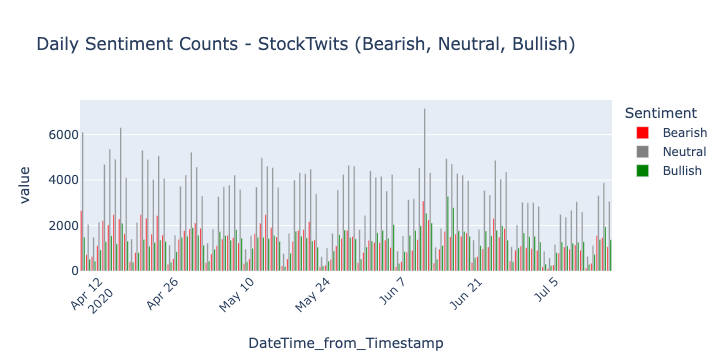
\includegraphics[width=\linewidth,height=0.6\textheight,keepaspectratio]{gfx/m4l3_notes_fig1_stocktwits_sentiment_counts.png}
\par\smallskip{\small \textbf{Hình 3.1:} Số lượng cảm xúc hàng ngày trên StockTwits (Bearish, Neutral, Bullish)}
\end{figure}

Cách tiếp cận này cho phép trực quan hóa các xu hướng cảm xúc hàng ngày trên StockTwits, với cách biểu diễn mã hóa màu rõ ràng cho các cảm xúc Bearish, Neutral và Bullish, giúp tăng khả năng diễn giải của biểu đồ. Biểu đồ cột trực quan hóa số lượng cảm xúc hàng ngày của các tin nhắn StockTwits về SPY ETF, được phân loại là Bearish (đỏ), Neutral (xám) hoặc Bullish (xanh lá). Trục hoành biểu diễn các ngày, còn trục tung biểu diễn số lượng tin nhắn. Ba cột cho mỗi ngày thể hiện số lượng của từng cảm xúc. Tính tương tác của Plotly cho phép phóng to, di chuột để xem chi tiết và khả năng chọn dữ liệu, cho phép khảo sát sâu các xu hướng cảm xúc theo thời gian.

\subsection{Phát hiện mã cổ phiếu trong dữ liệu StockTwits}

Các tin nhắn StockTwits thường chứa các mã cổ phiếu, còn được gọi là ticker hoặc cashtag. Người dùng thường đưa chúng vào để chỉ các cổ phiếu cụ thể mà họ đang thảo luận. Các mã này thường được biểu diễn bằng dấu đô la theo sau là mã chứng khoán của cổ phiếu (ví dụ \$AAPL cho Apple, \$SPY cho SPDR S\&P 500 ETF Trust).

Tương tự cách ta đã làm với tập dữ liệu Twitter, ở đây ta cũng có thể trích xuất các mã cổ phiếu từ các tin nhắn StockTwits. Đoạn mã dưới đây nhằm trích xuất các mã cổ phiếu (ticker) từ cột 'Sentence' của DataFrame \texttt{filtered\_stocktwits\_df}, đếm số lần xuất hiện của chúng và hiển thị 10 ticker được đề cập thường xuyên nhất:

\begin{lstlisting}[language=Python,escapeinside={(*@}{@*)}]
# (*@Phát@*) (*@hiện@*) (*@mã@*) (*@cổ@*) (*@phiếu@*) trong (*@dữ@*) (*@liệu@*) StockTwits
filtered_stocktwits_df['tickers'] = filtered_stocktwits_df['Sentence'].str.findall('\$[a-zA-Z]+\.*[a-zA-Z]+')
filtered_stocktwits_df.explode(['tickers'])['tickers'].value_counts().sort_values(ascending=False).head(10)
\end{lstlisting}

\begin{lstlisting}[escapeinside={(*@}{@*)}]
tickers
$SPY     553357
$QQQ      27869
$spy      12975
$SPX      11136
$AAPL     10631
$DJIA      8977
$DIA       8949
$ES        8062
$TSLA      7627
$BA        5368
Name: count, dtype: int64
\end{lstlisting}

Bảng này cho thấy 10 mã cổ phiếu (ticker) được đề cập thường xuyên nhất trong tập dữ liệu StockTwits, cùng với số lần xuất hiện tương ứng. Quan sát nổi bật nhất là sự thống trị của SPY: ticker \$SPY (SPDR S\&P 500 ETF Trust) và \$spy (phiên bản chữ thường của nó) là mã cổ phiếu được đề cập nhiều nhất với khoảng cách rất xa trong tập dữ liệu, xuất hiện hơn 553.000 lần. Điều này không đáng ngạc nhiên khi toàn bộ tập dữ liệu StockTwits này xoay quanh SPY.

Bảng cho thấy tập dữ liệu StockTwits chủ yếu tập trung vào các thảo luận về chỉ số S\&P 500 và các ETF liên quan. Tuy nhiên, cũng có sự quan tâm đáng kể đến các chỉ số thị trường lớn khác, các cổ phiếu riêng lẻ (đặc biệt là các công ty vốn hóa lớn) và các hợp đồng tương lai. Thông tin này cung cấp hiểu biết về các chủ đề và xu hướng phổ biến nhất trong cộng đồng StockTwits trong giai đoạn được phân tích.

\subsection{So sánh dữ liệu Twitter và StockTwits}

Bây giờ hãy so sánh dữ liệu Twitter và StockTwits. Đoạn mã dưới đây nhằm thực hiện việc này bằng cách tạo một biểu đồ đường. Trước hết ta tính số lượng tweet hàng ngày từ DataFrame \texttt{filtered\_twitter\_df} bằng cách nhóm dữ liệu theo phần ngày của cột 'created\_at' (dùng \texttt{dt.date} để trích xuất ngày) rồi đếm số tweet trong mỗi nhóm bằng cách đếm các giá trị không rỗng trong cột 'tweet\_text'. Ta thực hiện thao tác tương tự với DataFrame \texttt{filtered\_stocktwits\_df}, dùng cột 'DateTime\_from\_Timestamp' để nhóm theo ngày và cột 'Sentence' để đếm tin nhắn. Sau đó ta tạo và tùy chỉnh biểu đồ:

\begin{lstlisting}[language=Python,escapeinside={(*@}{@*)}]
# (*@Nhóm@*) (*@dữ@*) (*@liệu@*) Twitter theo (*@ngày@*) (*@và@*) (*@đếm@*) tweet
daily_tweet_counts_twitter = filtered_twitter_df.groupby(filtered_twitter_df['created_at'].dt.date)['tweet_text'].count()

# (*@Nhóm@*) (*@dữ@*) (*@liệu@*) StockTwits theo (*@ngày@*) (*@và@*) (*@đếm@*) tin (*@nhắn@*)
daily_tweet_counts_stocktwits = filtered_stocktwits_df.groupby(filtered_stocktwits_df['DateTime_from_Timestamp'].dt.date)['Sentence'].count()

# # (*@Tạo@*) (*@một@*) (*@hình@*) (*@và@*) (*@vẽ@*) (*@dữ@*) (*@liệu@*) Twitter (*@và@*) StockTwits
plt.figure(figsize=(12, 6))
plt.plot(daily_tweet_counts_twitter.index, daily_tweet_counts_twitter.values, label='Twitter', marker='o')
plt.plot(daily_tweet_counts_stocktwits.index, daily_tweet_counts_stocktwits.values, label='StockTwits', marker='x')

# (*@Tùy@*) (*@chỉnh@*) (*@biểu@*) (*@đồ@*)
plt.xlabel('Date')
plt.ylabel('Number of Tweets')
plt.title('Daily Tweet Counts - Twitter vs. StockTwits')
plt.legend()
plt.grid(True)

# Xoay (*@nhãn@*) (*@trục@*) x (*@để@*) (*@dễ@*) (*@đọc@*) (*@hơn@*)
plt.xticks(rotation=45, ha='right')

# (*@Điều@*) (*@chỉnh@*) (*@bố@*) (*@cục@*) (*@để@*) (*@tránh@*) (*@nhãn@*) (*@chồng@*) (*@chéo@*) (*@và@*) (*@hiển@*) (*@thị@*) (*@biểu@*) (*@đồ@*)
plt.tight_layout()
plt.show()
\end{lstlisting}

\begin{figure}[H]
\centering
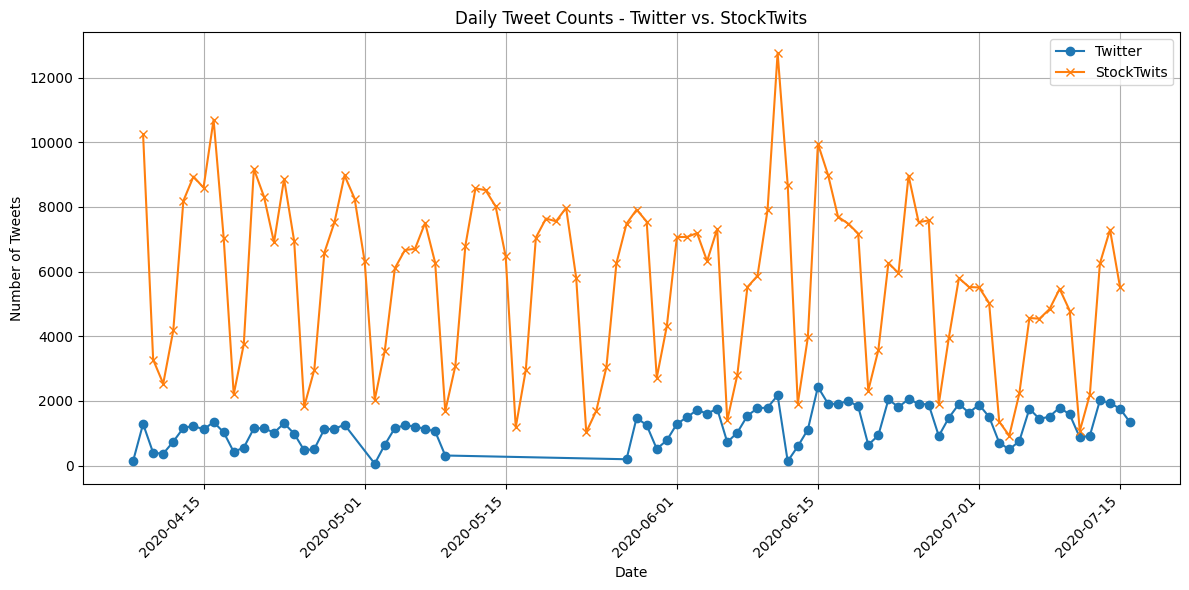
\includegraphics[width=\linewidth,height=0.6\textheight,keepaspectratio]{gfx/m4l3_notes_fig2_twitter_vs_stocktwits_daily_counts.png}
\par\smallskip{\small \textbf{Hình 3.2:} Số lượng tweet hàng ngày, Twitter so với StockTwits}
\end{figure}

Trước hết hãy quan sát rằng, trong cùng một giai đoạn, \texttt{filtered\_twitter\_df} có 99.246 hàng, trong khi \texttt{filtered\_stocktwits\_df} có 564.588 hàng. Thông tin này cung cấp ngữ cảnh có giá trị để diễn giải các biểu đồ số lượng tweet hàng ngày. Nó làm nổi bật sự khác biệt đáng kể về khối lượng dữ liệu giữa hai nền tảng trong giai đoạn đã chọn. Dưới đây là một số điểm bổ sung cần lưu ý:

\begin{itemize}
  \item Hoạt động của nền tảng: Sự khác biệt về số hàng cho thấy StockTwits có thể có hoạt động hoặc mức độ tương tác của người dùng cao hơn nhiều so với Twitter trong giai đoạn và tiêu chí lọc đã cho. Điều này có thể do nhiều yếu tố, bao gồm cơ sở người dùng, trọng tâm và mức độ phổ biến của các nền tảng trong cộng đồng đầu tư.
  \item Thu thập dữ liệu và tính toàn vẹn: Sự khác biệt về khối lượng dữ liệu có thể chịu ảnh hưởng của các phương pháp thu thập dữ liệu được sử dụng. Những người thu thập dữ liệu dùng các API hoặc nguồn dữ liệu khác nhau cho Twitter và StockTwits, và có thể có những khác biệt trong cách dữ liệu được thu thập, lọc hoặc xử lý, dẫn đến khác biệt về số hàng cuối cùng. Chúng ta cũng cần bảo đảm rằng các quy trình thu thập và lọc dữ liệu nhất quán và đáng tin cậy cho cả hai nền tảng để giảm thiểu các thiên lệch hoặc sai sót tiềm ẩn trong phân tích.
  \item Hàm ý cho phân tích: Khi so sánh các xu hướng hoặc mẫu hình giữa Twitter và StockTwits, cần lưu ý rằng số lượng tweet tuyệt đối có thể không so sánh trực tiếp được do khác biệt về khối lượng dữ liệu. Chúng ta cần cân nhắc dùng chuẩn hóa hoặc các thước đo tương đối để có những so sánh có ý nghĩa hơn.
  \item Ngữ cảnh của khoảng trống dữ liệu: Dù khoảng trống trong dữ liệu Twitter từ ngày 10 tháng 5 đến ngày 27 tháng 5 năm 2020 là điều quan trọng cần ghi nhận, cũng thiết yếu phải xem xét nó trong ngữ cảnh của tổng khối lượng dữ liệu. Nếu khoảng trống chiếm một tỷ lệ nhỏ trong tổng dữ liệu Twitter, tác động của nó lên phân tích tổng thể có thể hạn chế. Tuy nhiên, nếu khoảng trống là đáng kể so với tổng dữ liệu, nó có thể ảnh hưởng đến việc diễn giải các xu hướng hoặc mẫu hình.
\end{itemize}

Bằng cách xem xét sự khác biệt về tổng khối lượng dữ liệu và những hàm ý tiềm ẩn của nó, chúng ta có thể đưa ra các diễn giải có căn cứ hơn về các biểu đồ số lượng tweet hàng ngày và rút ra những kết luận vững chắc hơn từ phân tích. Chúng ta cần nhớ truyền đạt rõ ràng sự khác biệt về khối lượng dữ liệu cùng mọi phép chuẩn hóa hoặc điều chỉnh tỷ lệ đã áp dụng trong các báo cáo hoặc bài thuyết trình để bảo đảm tính minh bạch.

\section{Kết luận}

Trong bài học này, chúng ta đã khám phá các ứng dụng của dữ liệu thay thế. Dữ liệu thay thế trong tài chính là những nguồn dữ liệu phi truyền thống được dùng để thu được hiểu biết về xu hướng thị trường, định giá tài sản và các quyết định đầu tư. Điều này đối lập với dữ liệu truyền thống như báo cáo tài chính, hồ sơ công bố của công ty và giá thị trường. Dữ liệu văn bản từ mạng xã hội thuộc nhóm này vì nó phản ánh cảm xúc của công chúng, các bàn tán trên thị trường và sự lan truyền tin tức, những yếu tố có thể ảnh hưởng đến giá tài sản. Cụ thể, dữ liệu Twitter và StockTwits được xem là những nguồn dữ liệu thay thế có giá trị trong kỹ thuật tài chính nhờ tính thời gian thực và trọng tâm vào các thảo luận tài chính và hoạt động của thị trường chứng khoán.

Trong bài học này, chúng ta đã khám phá và so sánh dữ liệu Twitter và StockTwits để xem chúng có thể được dùng như thế nào cho phân tích tài chính. Trọng tâm chính là SPY ETF (SPDR S\&P 500 ETF Trust) và một khoảng thời gian cụ thể. Việc này bao gồm lấy dữ liệu từ cả Twitter và StockTwits, điều chỉnh múi giờ và xử lý retweet trên Twitter; tạo các biểu đồ để xem có bao nhiêu tweet được đăng mỗi ngày trên từng nền tảng nhằm hiểu sự khác biệt về khối lượng dữ liệu và hoạt động của người dùng.

\textbf{Tài liệu tham khảo}

\begin{itemize}
  \item Bruno Taborda, Ana de Almeida, José Carlos Dias, Fernando Batista, Ricardo Ribeiro, April 15, 2021, ``Stock Market Tweets Data'', IEEE Dataport, doi: \url{https://dx.doi.org/10.21227/g8vy-5w61}
  \item Liu, Jin-Xian (2022). SPY\_stocktwits\_messages.csv. figshare. Dataset. \url{https://doi.org/10.6084/m9.figshare.20237736.v1}
\end{itemize}

\chapter{Đọc thêm 1: SA-MAIS, Bộ Phân tích Cảm xúc Lai cho Thị trường Chứng khoán (Taborda et al.)}
\label{ch:M4L3DT1}

% Nguồn: Taborda, B., et al. ``SA-MAIS: Hybrid automatic sentiment analyser for stock market.'' Journal of Information Science, 2023.
% Phần cần đọc: Toàn bộ bài báo
% Nội dung bắt buộc đọc: được kiểm tra trong mọi bài đánh giá (kể cả Quiz).

\section{Thông tin nguồn}

\begin{itemize}
  \item \textbf{Nguồn:} Taborda, B., Maria de Almeida, A., Carlos Dias, J., Batista, F., \& Ribeiro, R. \emph{SA-MAIS: Hybrid automatic sentiment analyser for stock market}. Journal of Information Science, 2023. \url{https://doi.org/10.1177/01655515231171361}
  \item \textbf{Phần cần đọc:} Toàn bộ nội dung
\end{itemize}

\bigskip
\noindent\textbf{Bruno Taborda}\\
{\small Instituto Universitário de Lisboa (ISCTE-IUL), Bồ Đào Nha; Centre for Informatics and Systems of the University of Coimbra (CISUC), Bồ Đào Nha}

\noindent\textbf{Ana Maria de Almeida}\\
{\small Instituto Universitário de Lisboa (ISCTE-IUL), ISTAR, Bồ Đào Nha; Centre for Informatics and Systems of the University of Coimbra (CISUC), Bồ Đào Nha}

\noindent\textbf{José Carlos Dias}\\
{\small Instituto Universitário de Lisboa (ISCTE-IUL), Bồ Đào Nha; Business Research Unit (BRU-IUL), Bồ Đào Nha}

\noindent\textbf{Fernando Batista}\\
{\small Instituto Universitário de Lisboa (ISCTE-IUL), Bồ Đào Nha; INESC-ID Lisboa, Bồ Đào Nha}

\noindent\textbf{Ricardo Ribeiro}\\
{\small Instituto Universitário de Lisboa (ISCTE-IUL), Bồ Đào Nha; INESC-ID Lisboa, Bồ Đào Nha}

\bigskip
{\small \textbf{Tác giả liên hệ:} Bruno Taborda, ISTAR, Instituto Universitário de Lisboa (ISCTE-IUL), Lisbon 1649-026, Bồ Đào Nha. Email: Bruno\_Taborda@iscte-iul.pt}

\section{Tóm tắt}

Phân tích cảm xúc (sentiment analysis) đối với các tweet liên quan đến thị trường chứng khoán là một nhiệm vụ đầy thách thức, không chỉ vì tính đặc thù của lĩnh vực mà còn vì bản chất ngắn gọn của văn bản. Nghiên cứu này đề xuất SA-MAIS, một phương pháp hai bước nhẹ, được thiết kế riêng để thực hiện phân tích cảm xúc trong các tin nhắn văn bản ngắn bị giới hạn theo lĩnh vực. Để giải quyết vấn đề đặc thù lĩnh vực, dựa trên tần suất xuất hiện của từ, các từ liên quan nhất được tự động trích xuất từ lĩnh vực mới rồi được gắn nhãn thủ công để cập nhật một từ điển cảm xúc (lexicon) đặc thù lĩnh vực đã có sẵn. Sau đó, cảm xúc được phân loại bằng cách kết hợp từ điển đặc thù lĩnh vực đã cập nhật với VADER, một công cụ phân tích cảm xúc nổi tiếng và được sử dụng rộng rãi. Phương pháp đề xuất được so sánh với các công cụ phân tích cảm xúc nổi tiếng và được sử dụng rộng rãi khác, bao gồm các mô hình dựa trên transformer như BERTweet, Twitter-roBERTa và FinBERT, trên một tập dữ liệu chuyên biệt gồm 1 triệu tweet liên quan đến thị trường chứng khoán. Kết quả thực nghiệm cho thấy phương pháp đề xuất vượt trội đáng kể so với các công cụ phân tích cảm xúc khác, đạt độ chính xác tổng thể 72.0\%. Các kết quả đạt được làm nổi bật lợi thế của việc sử dụng một phương pháp lai kết hợp từ điển đặc thù lĩnh vực với các công cụ tổng quát sẵn có để suy luận cảm xúc trong các tin nhắn văn bản ngắn liên quan đến thị trường chứng khoán.

\subsection*{Từ khóa}
Phân tích cảm xúc (sentiment analysis); phân loại cảm xúc; từ điển cảm xúc (sentiment lexicon); thị trường chứng khoán; tweet

\section{1. Giới thiệu}

Mạng xã hội Twitter được tạo ra vào năm 2006 và hiện nay được sử dụng rộng rãi, với khoảng 500 triệu tweet mỗi ngày, bao trùm mọi loại nội dung. Do đó, Twitter được dùng phổ biến để phân tích cách biểu đạt cảm xúc trong dữ liệu văn bản [1\textendash 3]. Do giới hạn tối đa 280 ký tự của một tweet, tác giả cần diễn đạt quan điểm một cách trực diện. Khi tweet xuất phát từ các lĩnh vực chuyên môn cụ thể, người dùng thường sử dụng thuật ngữ kỹ thuật và các từ đa nghĩa, mà ý nghĩa của chúng chỉ được hiểu đúng trong bối cảnh cụ thể của tweet đó. Vì vậy, hiện nay, phân tích cảm xúc của các tweet đặc thù lĩnh vực được coi là một nhiệm vụ đầy thách thức [4].

Phân tích cảm xúc, một nhiệm vụ liên quan đến xử lý ngôn ngữ tự nhiên (natural language processing, NLP), sử dụng nhiều phương pháp và công cụ để tự động phát hiện thông tin liên quan từ một văn bản nhằm xác định cảm xúc hoặc quan điểm chủ đạo mà nó thể hiện [5]. Cách tiếp cận phổ biến nhất cho phân tích cảm xúc hoặc phát hiện phân cực là phân loại cảm xúc thành tích cực, trung lập hoặc tiêu cực [6]. Để thực hiện phân tích cảm xúc, và vì đây là một nhiệm vụ phụ thuộc nhiều vào lĩnh vực, kiến thức đặc thù lĩnh vực đóng vai trò then chốt để đạt được hiệu suất phân loại tốt [7]. Phần lớn các nghiên cứu hiện có về phân tích cảm xúc văn bản áp dụng các công cụ được xây dựng cho lĩnh vực tổng quát [8, 9], dẫn đến hiệu suất thấp hơn. Lý do là phân tích cảm xúc phụ thuộc vào lĩnh vực: các từ đặc thù lĩnh vực không được tính đến, và cùng một từ có thể biểu đạt cảm xúc khác nhau tùy lĩnh vực. Trên thực tế, chỉ có rất ít phương pháp được thiết kế riêng cho các lĩnh vực tài chính và thị trường chứng khoán [10\textendash 12]. Sử dụng độc lập một từ điển đặc thù lĩnh vực có những hạn chế nhất định, do nó được xây dựng dựa trên một tập dữ liệu cụ thể và tương đối nhỏ. Để khắc phục những hạn chế này, một vài công trình đã thử kết hợp từ điển tổng quát và từ điển đặc thù lĩnh vực nhằm cung cấp một bộ phân loại cảm xúc tốt hơn [13\textendash 15]. Mặc dù các từ điển tổng quát, đặc thù lĩnh vực hoặc lai đã được sử dụng rộng rãi, chúng tôi không tìm thấy nghiên cứu nào tạo ra một từ điển đặc thù và cập nhật để đánh giá cảm xúc của các tweet liên quan đến thị trường chứng khoán.

Nghiên cứu này tìm hiểu: (a) liệu phân tích cảm xúc cho các tweet thị trường chứng khoán có thể được cải thiện bằng cách sử dụng một từ điển thị trường chứng khoán được xây dựng riêng một cách tự động từ Twitter hay không, và (b) hiệu suất phân tích cảm xúc của các tweet thị trường chứng khoán bị ảnh hưởng như thế nào khi sử dụng các từ điển lai so với các cách tiếp cận tổng quát. Hơn nữa, chúng tôi trình bày một bản cải tiến cho từ điển tài chính tham chiếu hiện có, từ điển Loughran\textendash McDonald (LMcD) [10]. Từ điển được cập nhật này, LMcD20, chứa thêm các từ chưa từng được đưa vào từ điển trước đó và được tự động rút trích từ một kho ngữ liệu gồm các tweet gần đây liên quan đến thị trường chứng khoán. Chúng tôi cũng mở rộng kho tri thức hiện có bằng cách đề xuất SA-MAIS: một phương pháp lai cho phân tích cảm xúc của văn bản đặc thù lĩnh vực, tích hợp các từ điển tổng quát với một từ điển cảm xúc đặc thù lĩnh vực đã được cập nhật. Phương pháp này cho kết quả so sánh tích cực với các công cụ hiện có. Các thực nghiệm của chúng tôi cho thấy cách tiếp cận sáng tạo này đạt kết quả tốt hơn so với các mô hình đã được huấn luyện sẵn hoặc việc sử dụng độc lập các từ điển tổng quát hoặc chuyên biệt. SA-MAIS được công bố trên GitHub,\footnote{https://github.com/taborda11/SAMAIS.} và tập dữ liệu dùng để kiểm định SA-MAIS cũng như tăng cường LMcD được công bố trên IEEE DataPort.\footnote{https://ieee-dataport.org/open-access/stock-market-tweets-data.}

Phần còn lại của bài báo được tổ chức như sau: sau phần giới thiệu, một tổng quan ngắn gọn về các nghiên cứu liên quan quan trọng nhất được trình bày trong mục 2. Mục 3 trình bày mục tiêu nghiên cứu và các câu hỏi nghiên cứu. Mục 4 trình bày tập dữ liệu và kiến trúc của hệ thống SA-MAIS. Mục 5 trình bày chi tiết việc cải tiến từ điển đặc thù lĩnh vực. Mục 6 mô tả việc triển khai SA-MAIS. Mục 7 làm nổi bật các hàm ý về lý thuyết và thực tiễn cũng như những hạn chế của nghiên cứu này. Mục 8 thảo luận các hướng nghiên cứu tiếp theo có thể thực hiện và trình bày các kết luận chính của nghiên cứu.

\section{2. Tổng quan tài liệu}

Phân tích cảm xúc, còn được gọi là phân tích quan điểm (opinion analysis) [16], sử dụng NLP và phân tích văn bản để khám phá giá trị cảm xúc (valence) trong dữ liệu văn bản (ví dụ: tài liệu, tweet và tin nhắn trực tiếp). Nhìn chung, phân tích cảm xúc nhằm đánh giá tính khách quan hoặc chủ quan của một văn bản và phân loại nó là tích cực hoặc tiêu cực, nên loại phân loại này được coi là bài toán nhị phân [17, 18]. Saif et al. [19] đã tạo ra SentiCircle, một biểu diễn cảm xúc ngữ nghĩa (semantic sentiment representation) của các từ. Phương pháp này nắm bắt dữ liệu ngữ cảnh, dựa trên tần suất xuất hiện của tweet và cập nhật cảm xúc dựa trên ngữ nghĩa ngữ cảnh.

Nofsinger [20] kết luận rằng, do bản chất của cổ phiếu, thị trường chứng khoán chịu tác động trực tiếp bởi tâm trạng xã hội, và hành vi này của thị trường có thể giúp dự báo ``hoạt động tài chính và kinh tế''. Sul et al. [21] thu thập các tweet có đề cập đến mã cổ phiếu (như AAPL cho Apple Inc.) của các công ty thuộc S\&P 500 và phân loại cảm xúc trong từng tweet là tích cực hoặc tiêu cực. Các tác giả cũng chỉ ra rằng phân tích cảm xúc của họ có liên quan đến lợi suất cổ phiếu của công ty. Họ cũng chứng minh rằng người dùng có nhiều người theo dõi tác động trực tiếp đến lợi suất trong cùng ngày, trong khi người dùng có ít người theo dõi hơn tác động đến lợi suất trong tương lai (lợi suất sau 10 ngày). Tóm lại, phần lớn các nghiên cứu trước đây đều ủng hộ quan điểm rằng tâm trạng công chúng và cảm xúc được thể hiện qua truyền miệng (word-of-mouth, WOM) tác động đến giá cổ phiếu trên thị trường. Bollen et al. [22] xây dựng một hệ thống tương quan giữa chỉ số Dow Jones Industrial Average với dữ liệu Twitter. Chandra Pandey et al. [23] đề xuất một phương pháp phân cụm mới để đánh giá cảm xúc của tweet. Phương pháp đề xuất vượt trội hơn năm thuật toán nổi tiếng nhất. Trong một nghiên cứu gần đây hơn, Song et al. [4] mô tả một kỹ thuật kết hợp học có giám sát và học không giám sát, sử dụng một mô hình biểu diễn văn bản mới có tên Word2PLTS cho phân tích cảm xúc văn bản ngắn. Mô hình này dựa trên các tập thuật ngữ ngôn ngữ xác suất (probabilistic linguistic term sets) mô tả đầy đủ các khả năng về phân cực của từ.

Hu et al. [24] đề xuất một phương pháp tóm tắt nhiệm vụ xác minh thủ công các đánh giá của khách hàng bằng cách xem xét các đặc điểm liên quan đến sản phẩm trong tập dữ liệu. Các tác giả đã tạo ra một từ điển đặc thù lĩnh vực cho các đánh giá của khách hàng như một nỗ lực nhằm tăng hiệu suất của từ điển họ xây dựng. Loughran et al. [10] nhận thấy rằng các phương pháp trước đây phân loại sai văn bản tài chính. Do đó, các tác giả đã tạo ra một từ điển đặc thù lĩnh vực để phân loại cảm xúc của các văn bản tài chính chính xác hơn. Tuy nhiên, Li et al. [25] đã triển khai một ``khung dự đoán giá cổ phiếu tổng quát'' sử dụng từ điển Harvard IV-4 và từ điển cảm xúc tài chính Loughran\textendash McDonald [10] cho phân tích cảm xúc. Khung tổng quát được đề xuất đã được kiểm định bằng 5 năm dữ liệu lịch sử về giá cả và tin tức trên Sở Giao dịch Chứng khoán Hồng Kông. Các tác giả kết luận rằng các mô hình chỉ tập trung vào các lớp cảm xúc tích cực và tiêu cực không cho ra dự đoán tốt. Junqué et al. [26] sử dụng các bài báo từ tất cả các tờ báo lớn của Flanders trong khoảng thời gian từ 2007 đến tháng 3 năm 2012. Các tác giả kết luận rằng phân tích cảm xúc sử dụng Pattern cho Python [27], một gói Python với nhiều chức năng bao gồm xử lý ngôn ngữ tự nhiên, cho hiệu suất kém hơn so với Bag-Of-Words hoặc các chỉ báo kỹ thuật thị trường. Gần đây hơn, Oliveira et al. [28] chỉ ra rằng vẫn còn thiếu các từ điển tài chính được điều chỉnh cho các thị trường chứng khoán trên nền tảng tiểu blog (micro-blogging). Các tác giả đề xuất một quy trình tự động mới để tạo ra một từ điển dựa trên tập dữ liệu StockTwits.\footnote{https://stocktwits.com.}

Li et al. [29] kết hợp các chỉ báo kỹ thuật với tin tức làm nỗ lực dự đoán giá cổ phiếu tại Hồng Kông. Bốn từ điển được sử dụng để thực hiện phân tích cảm xúc trên các bài báo tin tức, cụ thể là Harvard IV-4 Dictionary, từ điển cảm xúc tài chính Loughran\textendash McDonald [10], SentiWordNet 3.0 [30] và SenticNet 5 [31]. Các tác giả kết luận rằng từ điển cảm xúc tài chính Loughran\textendash McDonald vượt trội hơn các từ điển còn lại.

Liên quan đến tính đặc thù của nội dung văn bản trong một tweet, một số tác giả sử dụng hashtag của Twitter (ví dụ: \#fail, \#iloveit), biểu tượng cảm xúc (ví dụ: :) và :\textbackslash) để đánh giá cảm xúc của tweet [32\textendash 34]. Sử dụng từ điển, Kiritchenko et al. [35] đã tạo ra một công cụ phân loại văn bản thống kê có giám sát nhằm phân tích cảm xúc của các tin nhắn văn bản ngắn (ví dụ: Twitter hoặc SMS), được các tác giả gọi là ``nhiệm vụ cấp thông điệp'' (message-level task), đồng thời phân tích cảm xúc của một từ hoặc cụm từ trong thông điệp, gọi là ``nhiệm vụ cấp thuật ngữ'' (term-level task). Các từ điển được tạo tự động bằng cách sử dụng tweet, hashtag và biểu tượng cảm xúc. Các tác giả kết luận rằng việc sử dụng các từ điển được tạo tự động cải thiện hiệu suất thêm 6.5\%. Về mặt các từ điển tài chính cụ thể, Oliveira et al. [28] sử dụng tần suất từ ngược tần suất tài liệu (term frequency\textendash inverse document frequency, TD-IDF), độ lợi thông tin, phần trăm lớp và xác suất lớp có trọng số để tạo ra một từ điển dựa trên StockTwits. Li et al. [36] sử dụng các bộ phân loại cảm xúc theo cụm bằng cách áp dụng phương pháp trọng số TD-IDF. Các tác giả kết luận rằng phương pháp này vượt trội hơn WordNet. Từ điển Cảm xúc WKWSCI [37] được tạo ra để đánh giá các bài đánh giá trên Amazon và được so sánh với sáu từ điển có sẵn: Hu \& Liu Opinion Lexicon, Multi-perspective Question Answering (MPQA) Subjectivity Lexicon, General Inquirer, National Research Council Canada (NRC) Word-Sentiment Association Lexicon và Semantic Orientation Calculator (SO-CAL) lexicon. Các tác giả kết luận rằng Từ điển Cảm xúc WKWSCI phù hợp nhất với văn bản phi đánh giá (non-reviews text). Hassan et al. [38] tạo ra một công cụ phân tích cảm xúc để đánh giá một tập dữ liệu Altmetrics. Các tác giả kết luận rằng máy vector hỗ trợ (support vector machine, SVM) với uni-gram vượt trội hơn hồi quy logistic và Naïve Bayes. Sohangir et al. [39] so sánh các công cụ dựa trên từ điển với các kỹ thuật học máy để thực hiện phân tích cảm xúc trong StockTwits. Các tác giả kết luận rằng VADER [9], một công cụ phân tích cảm xúc tổng quát, vượt trội hơn các công cụ dựa trên từ điển còn lại trong thực nghiệm, cụ thể là SentiWordNet và TextBlob. Ngoài ra, VADER cũng vượt trội hơn các kỹ thuật học máy như hồi quy logistic, SVM tuyến tính và phân loại Naïve Bayes.

Devlin et al. [40] đề xuất vào năm 2018 một mô hình được huấn luyện sẵn (pre-trained) mới có tên BERT, sử dụng biểu diễn mã hóa hai chiều từ transformer. Một trong những ưu điểm chính của mô hình này đến từ tính linh hoạt của nó, vì chỉ cần thêm một lớp đầu ra để tinh chỉnh (fine-tune) một mô hình BERT cho một nhiệm vụ cụ thể. Do đó, để tạo ra các mô hình mới bắt nguồn từ BERT, chỉ cần thêm một lớp đầu ra duy nhất. Quoc Nguyen et al. [41] đề xuất một mô hình BERT được tinh chỉnh cho phân tích cảm xúc tweet (BERTweet), một mô hình dựa trên BERT được huấn luyện với hơn 40,000 tweet. FinBERT được Araci [42] đề xuất dựa trên BERT, với mô hình được chuyên biệt hóa cho tin tức tài chính. FinBERT được huấn luyện với tin tức từ Reuters và các cơ sở dữ liệu financial phrase bank. Li et al. [43] sử dụng FinBERT để phân tích tiêu đề tin tức và so sánh với các mô hình bộ nhớ dài\textendash ngắn hạn (long short-term memory, LSTM) khác. Các tác giả kết luận rằng FinBERT vượt trội hơn các mô hình khác. roBERTa Twitter sentiment analyser (Twitter-roBERTa) là một mô hình dựa trên BERT, được huấn luyện trên hơn 58 triệu tweet và được tinh chỉnh với bộ chuẩn TweetEval do Barbieri et al. [44] đề xuất.

\section{3. Mục tiêu nghiên cứu}

Mục tiêu của chúng tôi là cung cấp một bằng chứng khái niệm (proof of concept) thông qua một nghiên cứu tình huống: đánh giá cảm xúc của các tweet liên quan trực tiếp đến thị trường chứng khoán.

Theo các tài liệu hiện có, phần lớn các công cụ cố gắng dự đoán hành vi thị trường sử dụng hoặc là các cách tiếp cận tổng quát hoặc các từ điển đặc thù lĩnh vực để định lượng cảm xúc của tweet hay các nguồn dữ liệu quan trọng khác (ví dụ: tin tức). Trong trường hợp cụ thể của các tweet liên quan đến thị trường chứng khoán, theo hiểu biết tốt nhất của chúng tôi, không có từ điển đặc thù lĩnh vực nào cho phân tích cảm xúc. Mục tiếp theo trình bày một phương pháp đơn giản mới để nâng cấp một từ điển tài chính hiện có. Về các công cụ tổng quát, chúng tôi đã lựa chọn sử dụng VADER, TextBlob và Stanza [8], cùng với các mô hình ngôn ngữ được huấn luyện chuyên biệt tiên tiến nhất là BERTweet [41], Twitter-roBERTa và FinBERT [42]. Các mô hình này đã được sử dụng trong các nghiên cứu gần đây nhất về phân tích cảm xúc, không chỉ trong các lĩnh vực tài chính [39] mà còn trong các lĩnh vực tổng quát [45].

Do đó, nghiên cứu này giải quyết các câu hỏi nghiên cứu sau đây:

\emph{RQ1.} Hiệu suất của các công cụ phân tích cảm xúc tổng quát có đủ tốt khi áp dụng để phân tích các tweet thị trường chứng khoán hay không?

\emph{RQ2.} Phân tích cảm xúc cho các tweet thị trường chứng khoán có thể được cải thiện bằng cách sử dụng các từ điển thị trường chứng khoán được xây dựng riêng hay không?

\emph{RQ3.} Phân tích cảm xúc của các tweet thị trường chứng khoán có thể được cải thiện bằng cách tích hợp một bộ phân tích tổng quát với một từ điển đặc thù lĩnh vực hay không?

Để trả lời các câu hỏi này, chúng tôi cho thấy rằng một phương pháp luận nhằm khám phá phân cực của các thông điệp văn bản ngắn trong một lĩnh vực cụ thể cần tích hợp kiến thức lĩnh vực được cập nhật.

\section{4. Phương pháp luận}

Trong quá trình phân tích tập dữ liệu của chúng tôi, có thể thấy rõ rằng một số từ như ``breakthrough'' (bước đột phá) và ``barred'' (bị cấm) không được các bộ phân tích cảm xúc tổng quát (generalist sentiment analysers, GSA) phân loại đầy đủ. Trong vài năm qua, hoặc là các từ điển đặc thù lĩnh vực hoặc các từ điển tổng quát đã được nghiên cứu để phân tích cảm xúc. Các ứng dụng khác nhau nhận thấy rằng nếu tập dữ liệu đủ cụ thể cho một chủ đề nhất định, chẳng hạn như tài chính, một từ điển đặc thù lĩnh vực có thể cải thiện kết quả. Chúng tôi giải quyết vấn đề này bằng cách đề xuất một cách tiếp cận mới, SA-MAIS, một bộ phân tích cảm xúc khác biệt với các công cụ trước đây vì nó kết hợp một công cụ tổng quát với một từ điển đặc thù lĩnh vực. Kiến trúc của hệ thống SA-MAIS được minh họa trong Hình 1. Các phương pháp và định nghĩa được tạo ra để triển khai hệ thống được trình bày chi tiết ở mục 6 sau này.

\begin{figure}[H]
\centering
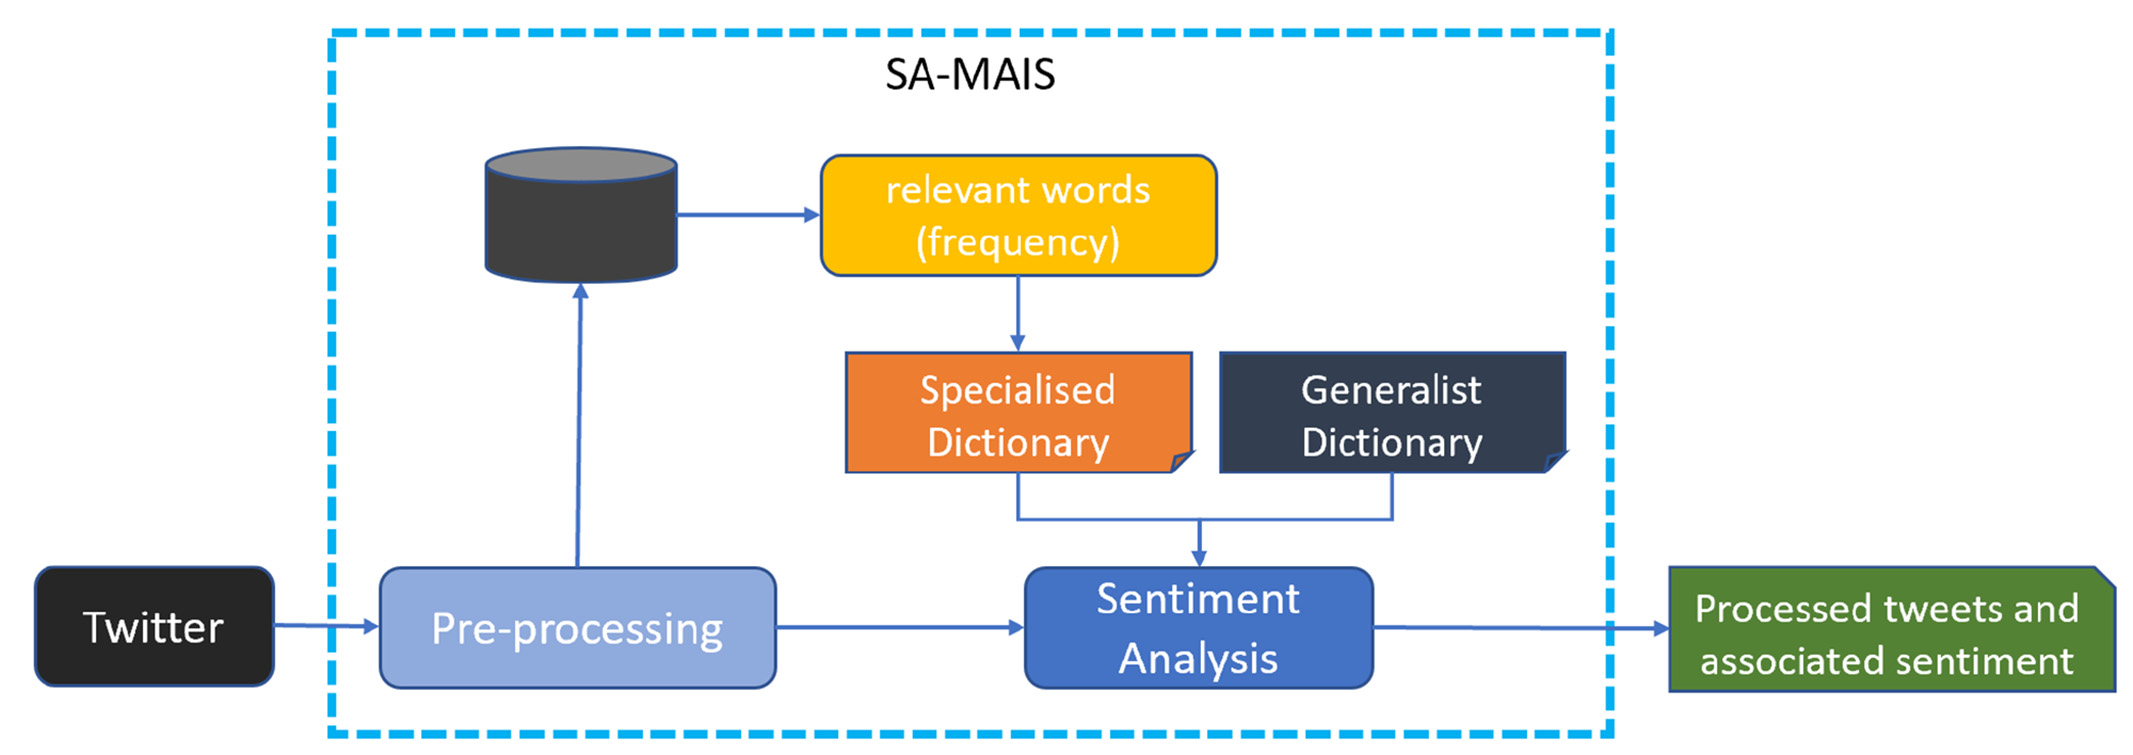
\includegraphics[width=0.85\linewidth]{gfx/m4l3_taborda_fig1_samais_architecture.png}
\par\smallskip{\small \textbf{Hình 1:} Kiến trúc hệ thống SA-MAIS.}
\end{figure}

Để kiểm định SA-MAIS như một bộ phân tích cảm xúc văn bản ngắn, chúng tôi khám phá và so sánh sáu bộ phân loại cảm xúc tổng quát nổi tiếng: TextBlob, Stanza, VADER, BERTweet, Twitter-roBERTa và FinBERT. Công cụ đầu tiên, TextBlob,\footnote{https://textblob.readthedocs.io.} là một thư viện Python được huấn luyện sẵn cho NLP, trả về hai giá trị cho phân tích cảm xúc: phân cực (polarity) của văn bản và tính chủ quan (subjectivity) của nó. Giá trị thứ hai là một thước đo mức độ thiếu tính khách quan và do đó mang tính trừu tượng, phụ thuộc vào nhận thức và quan điểm cá nhân, trong khi phân cực thể hiện cảm xúc tổng thể của tweet và được đánh giá trong khoảng $[-1.0, 1.0]$, với $-1.0$ là cảm xúc tiêu cực nhất và $1.0$ biểu thị cảm xúc hoàn toàn tích cực. Stanza [8] là một bộ công cụ được tạo ra vào năm 2020 tại Đại học Stanford để phân tích văn bản bằng nhiều ngôn ngữ (tiếng Anh, tiếng Đức và tiếng Trung). Bộ phân loại này được huấn luyện sử dụng 112 tập dữ liệu. Các giá trị phân cực khác với các giá trị trả về từ TextBlob vì Stanza trả về các giá trị 0, 1 và 2, đại diện tương ứng cho cảm xúc tiêu cực, trung lập và tích cực. Hutto và Gilbert [46] phát triển VADER, được coi là thư viện nhúng trong NLTK. Các tác giả mô tả VADER là ``một mô hình dựa trên quy tắc đơn giản cho phân tích cảm xúc tổng quát''. VADER đã được so sánh với các từ điển cảm xúc/quan điểm khác nhau: Linguistic Inquiry Word Count (LIWC), General Inquirer (GI), Affective Norms for English Words (ANEW), SentiWordNet (SWN), SenticNet (SCN) và Word-Sense Disambiguation (WSD) sử dụng WordNet. Các tác giả kết luận rằng VADER vượt trội hơn tất cả các từ điển khi phân loại văn bản mạng xã hội [9].

\begin{figure}[H]
\centering
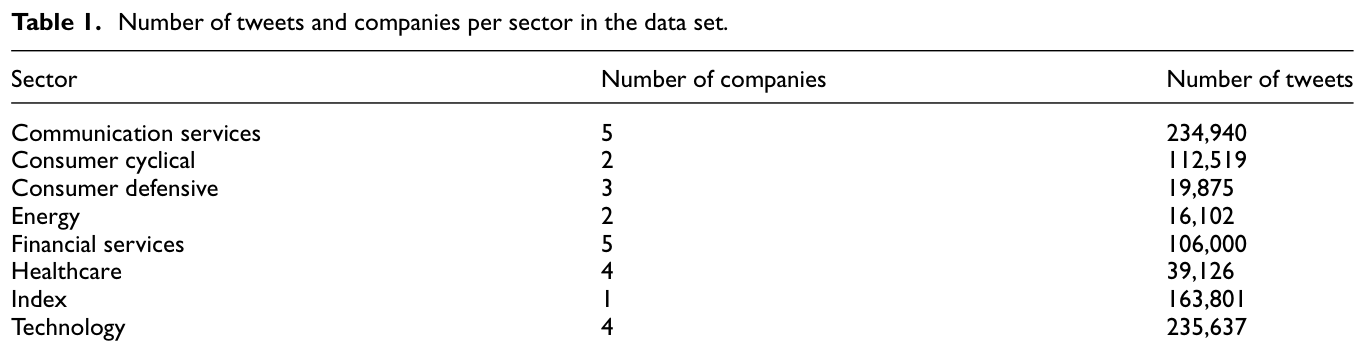
\includegraphics[width=0.9\linewidth]{gfx/m4l3_taborda_table1_tweets_per_sector.png}
\par\smallskip{\small \textbf{Bảng 1:} Số lượng tweet và số công ty theo từng ngành trong tập dữ liệu.}
\end{figure}

\begin{figure}[H]
\centering
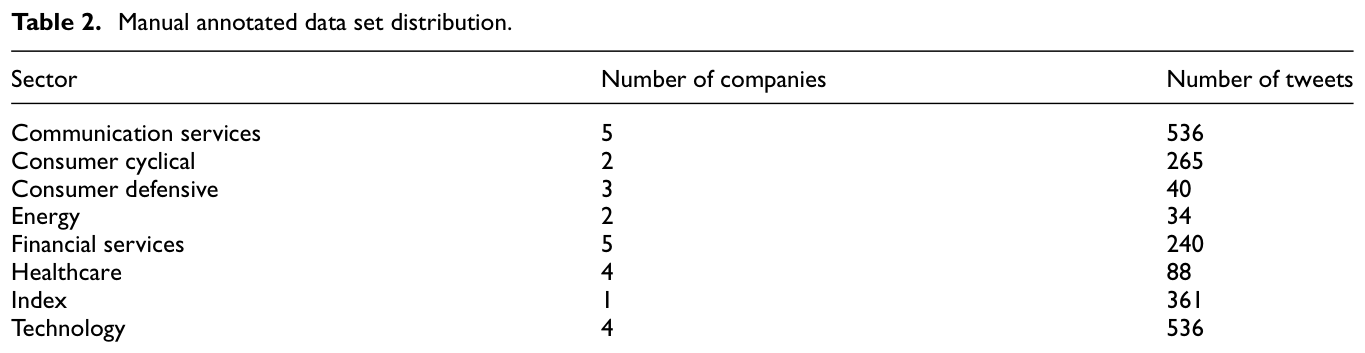
\includegraphics[width=0.9\linewidth]{gfx/m4l3_taborda_table2_annotated_data_distribution.png}
\par\smallskip{\small \textbf{Bảng 2:} Phân bố tập dữ liệu được gán nhãn thủ công.}
\end{figure}

BERTweet là một mô hình do Quoc Nguyen et al. [41] tạo ra, được huấn luyện với kho ngữ liệu SemEval 2017 (khoảng 40,000 tweet). Mô hình phân loại cảm xúc thành ba lớp khác nhau: POS, NEG và NEU, lần lượt đại diện cho cảm xúc tích cực, tiêu cực và trung lập. Twitter-roBERTa được huấn luyện trên khoảng 58 triệu tweet và được tinh chỉnh cho phân tích cảm xúc bằng bộ chuẩn TweetEval [44]. Mô hình đưa ra ba nhãn để phân loại cảm xúc, 0 đại diện cho cảm xúc tiêu cực, 1 đại diện cho cảm xúc trung lập và 2 đại diện cho cảm xúc tích cực. FinBERT được huấn luyện tinh chỉnh bằng Financial Phrasebank của Malo et al. [47]. Mô hình cho ra ba nhãn đầu ra: tích cực, tiêu cực và trung lập.

Cần lưu ý rằng, theo hiểu biết tốt nhất của chúng tôi, (1) không có tập dữ liệu tweet thị trường chứng khoán được gán nhãn thủ công cho ba lớp cảm xúc có thể có: tích cực, trung lập và tiêu cực. Hơn nữa, (2) không có bộ dữ liệu chuẩn (benchmark) với số lượng tweet đủ lớn liên quan đến S\&P500 và các công ty thành viên. Về vấn đề này, chúng tôi đã thu thập và lọc khoảng 928,000 tweet về thị trường chứng khoán, trong khoảng thời gian từ ngày 9 tháng 4 năm 2020 đến ngày 16 tháng 7 năm 2020, liên quan đến 25 công ty có khối lượng giao dịch cao nhất trong chỉ số S\&P 500 thông qua mã cổ phiếu (cash tag), \$SPX và \#stock. Khung thời gian này được sử dụng nhằm giảm khả năng xuất hiện các mô hình theo mùa/thời điểm (tức là xu hướng gia tăng của cảm xúc) có thể ảnh hưởng đến thực nghiệm và, do đó, ảnh hưởng đến kết quả. Bảng 1 cho thấy sự phân bố của các công ty và tweet theo từng ngành kinh tế.

Việc tạo ra một tập dữ liệu được gán nhãn cho một nhiệm vụ đặc thù lĩnh vực rất tốn thời gian và chịu ảnh hưởng lớn bởi tính chủ quan của người gán nhãn. Ví dụ, Li et al. [48] sử dụng hai tập dữ liệu được gán nhãn để đề xuất một phương pháp phân tích cảm xúc mới cho các đánh giá của người dùng bằng các mô hình học sâu. Cả hai tập dữ liệu đều có tập kiểm định, lần lượt với 2210 và 802 đánh giá. Mowlaei et al. [49] đề xuất một bộ phân tích cảm xúc theo khía cạnh (aspect-based sentiment analyser) mới. Để kiểm định mô hình này, các tác giả sử dụng một tập dữ liệu gồm 367 đánh giá tích cực và 267 đánh giá tiêu cực, tổng cộng 634 đánh giá. Chúng tôi không tìm thấy bất kỳ tập dữ liệu tweet nào được gán nhãn thủ công chuyên biệt cho lĩnh vực thị trường chứng khoán. Do đó, chúng tôi đã tự gán nhãn thủ công một mẫu ngẫu nhiên gồm 2100 tweet. Bảng 2 cho thấy sự phân bố công ty và tweet theo từng ngành kinh tế cho tập dữ liệu được gán nhãn thủ công này. Các tweet được phân loại thủ công bằng ba giá trị cảm xúc có sẵn: tích cực, trung lập và tiêu cực. Việc gán nhãn được thực hiện bởi hai người gán nhãn độc lập, là chuyên gia trong lĩnh vực thị trường chứng khoán, nhằm giảm tính chủ quan khi gán nhãn tập dữ liệu. Chỉ số kappa của Cohen [50] được sử dụng để định lượng mức độ đồng thuận giữa những người gán nhãn. Thước đo này nằm trong khoảng $[-1.0, 1.0]$, trong đó $1.0$ nghĩa là hoàn toàn đồng thuận giữa những người gán nhãn và $-1.0$ nghĩa là không có sự đồng thuận nào. Việc gán nhãn thủ công cho tập dữ liệu này đạt kappa 0.88, thể hiện mức độ đồng thuận gần như hoàn hảo giữa những người gán nhãn [50].

\section{5. Cải tiến từ điển cảm xúc}

Như đã chỉ ra trước đó, Loughran và McDonald đã tạo ra các danh sách cảm xúc dựa trên cách diễn giải khả dĩ nhất của một từ trong bối cảnh kinh doanh, tạo ra hai danh sách từ điển chứa 354 từ tích cực và 2329 từ tiêu cực [10]. Danh sách từ điển này từ đây được gọi là LMcD, hiện là một từ điển tài chính và kế toán tham chiếu [52]. Tuy nhiên, nó được xây dựng dựa trên các văn bản kế toán tài chính để tăng cường phân tích cảm xúc trong lĩnh vực đặc thù này.

Mục này mô tả các thay đổi được đưa vào từ điển LMcD nhằm cải thiện khả năng đại diện của nó cho việc phân tích thị trường chứng khoán (mục 5.1) và làm nổi bật các kết quả đạt được từ từ điển đã được tăng cường mới (mục 5.2).

\subsection*{5.1. LMcD20: cải tiến từ điển đặc thù lĩnh vực}

Một khảo sát sâu hơn về tập dữ liệu tweet thị trường chứng khoán thứ hai (tập dữ liệu chưa được gán nhãn) cho thấy một số từ đặc thù và phổ biến liên quan đến thị trường chứng khoán (như ``breakthrough'' và ``barred'') không được các công cụ phân tích cảm xúc tổng quát phân loại một cách phù hợp, cho thấy sự cần thiết phải sử dụng các từ điển đặc thù lĩnh vực. Tuy nhiên, một khảo sát chi tiết hơn về LMcD cũng cho thấy một số từ hiện đang được sử dụng trong các tweet tài chính vẫn chưa có mặt trong LMcD. Chúng tôi cũng nhận thấy rằng các từ dùng để bày tỏ quan điểm trên Twitter chịu ảnh hưởng của cách diễn giải chủ quan và thay đổi theo thời gian. Do đó, một từ điển đặc thù lĩnh vực cho Twitter không thể là tĩnh mà cần được điều chỉnh theo thời gian dựa trên nội dung từ vựng thực tế và cập nhật.

Để giải quyết vấn đề này, chúng tôi đã sử dụng dữ liệu tweet thị trường chứng khoán chứa dữ liệu mới hơn như một phương tiện để cải thiện từ điển của mình. Một mẫu các từ tích cực và tiêu cực chưa có trong LMcD được chọn từ 500 từ phổ biến nhất được trích xuất từ tập dữ liệu quy mô lớn. Trong số đó, 23 từ thể hiện cảm xúc tích cực (như ``buy'' hoặc ``bull'') và 13 từ thể hiện cảm xúc tiêu cực (như ``short'' hoặc ``bear''). Các tác giả đã lựa chọn thủ công các từ thể hiện cảm xúc, dẫn đến 36 từ mới liên quan đến tài chính (Bảng 3) được thêm vào từ điển LMcD, từ đó tạo ra LMcD20.

\begin{figure}[H]
\centering
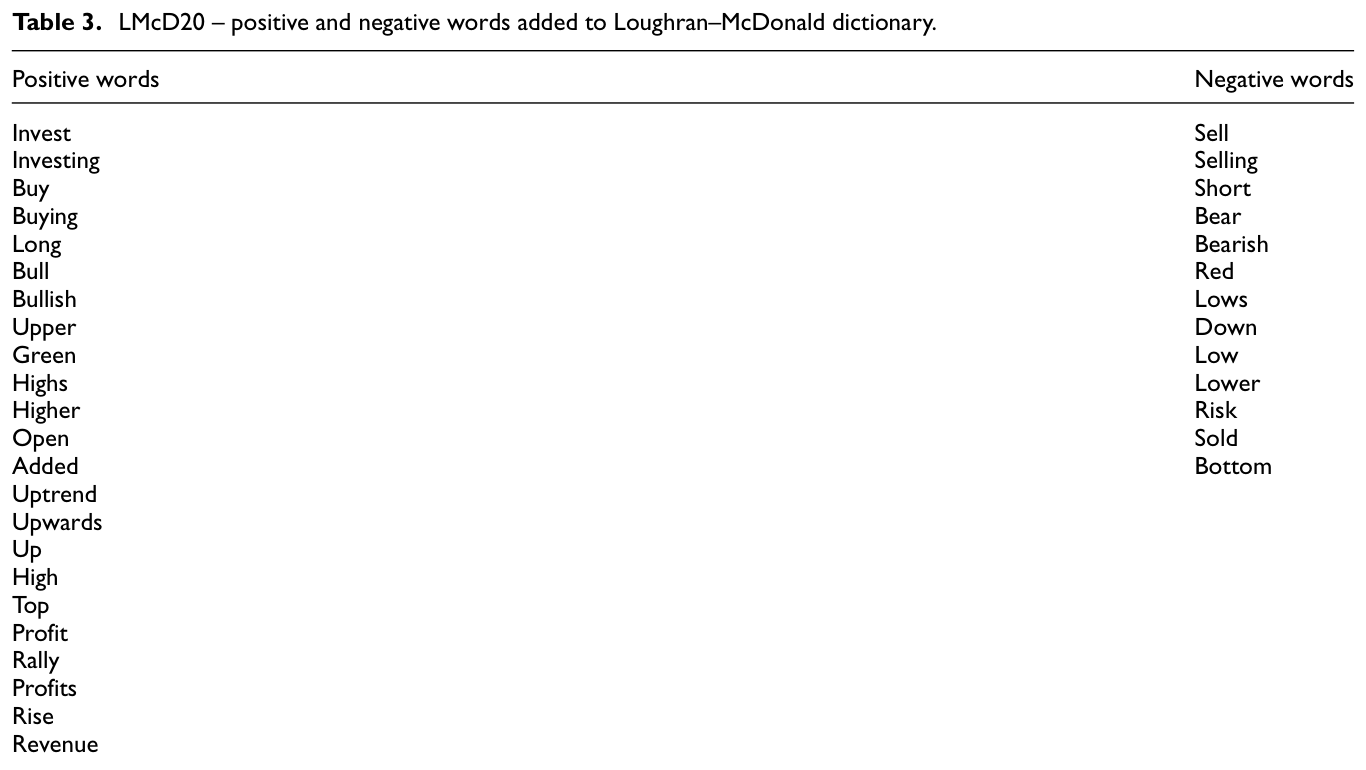
\includegraphics[width=0.85\linewidth]{gfx/m4l3_taborda_table3_lmcd20_words.png}
\par\smallskip{\small \textbf{Bảng 3:} LMcD20, các từ tích cực và tiêu cực được thêm vào từ điển Loughran\textendash McDonald.}
\end{figure}

Để giữ cho SA-MAIS cập nhật nhất có thể dựa trên tần suất từ, chúng tôi đã tạo ra một tập dữ liệu khác với gần 1 triệu tweet, cung cấp dữ liệu chất lượng quy mô lớn cho việc phân tích. Cả hai tập dữ liệu đều đã được công bố công khai [51].

\subsection*{5.2. So sánh các từ điển khác nhau}

Để đánh giá mô hình, tức là kiểm định kết quả phân loại tích cực, tiêu cực hoặc trung lập của các từ, và do lớp tiêu cực mất cân bằng nhẹ so với các lớp còn lại, thước đo được chọn để so sánh các thực nghiệm là độ nhạy trung bình có trọng số (weighted average recall, WAR). Hàm này gán trọng số cho recall của từng lớp theo số lượng mẫu của lớp đó. WAR được định nghĩa theo phương trình (1), trong đó $TP_p$, $TP_n$ và $TP_t$ lần lượt là số lượng dự đoán đúng (true positive) liên quan đến lớp tích cực ($p$), lớp tiêu cực ($n$) và lớp trung lập ($t$), còn $N$ đại diện cho tổng số tweet:

\[
\text{WAR} = \frac{TP_p + TP_n + TP_t}{N} \qquad (1)
\]

Trong thực nghiệm ban đầu, chúng tôi đã thực hiện so sánh giữa các từ điển đặc thù lĩnh vực. Trong các từ điển đặc thù lĩnh vực, Hu et al. [24] (Sentilex) là một trong những từ điển nổi tiếng nhất và được tạo ra để phân tích các đánh giá của khách hàng. Oliveira et al. [11] (từ điển cảm xúc thị trường chứng khoán, SMSL) và Loughran và McDonald [10] (LMcD) là ví dụ về các từ điển tài chính được tạo ra để sử dụng trong các bối cảnh kinh tế cụ thể. Mohammad và Turney [53] (NRC) là một trong những từ điển đặc thù lĩnh vực nổi tiếng nhất kết hợp phân cực cảm xúc và cảm xúc trong cùng một từ điển cho một kịch bản huy động cộng đồng (crowd-sourcing). Loughran và McDonald tạo ra từ điển LMcD vào năm 2011 để đánh giá các báo cáo tài chính của các công ty. LMcD chứa hai tập con từ: tập từ tiêu cực, bao gồm 2329 từ, và tập từ tích cực, chứa 354 từ [10]. Nhiều từ liên quan đến thị trường tài chính có thể được tìm thấy trong từ điển, nhưng khác với tweet, các báo cáo tài chính được cấu trúc rất tốt và được viết cẩn thận.

Từ điển SMSL được tạo ra vào năm 2016 với mục tiêu chính là đánh giá cảm xúc StockTwits [11]. Từ điển này chứa 20,551 uni-gram và bi-gram và được tạo tự động dựa trên một mẫu StockTwits sử dụng phương pháp thống kê. Tuy vậy, việc kiểm định SMSL được thực hiện bằng cách sử dụng một lựa chọn gồm 5000 StockTwits được các tác giả của các bài đăng phân loại nhưng loại trừ cảm xúc trung lập. Mỗi $n$-gram ($n = 1, 2$) có một trọng số khác nhau tùy theo ngữ cảnh của câu tại thời điểm đó, mang tính tích cực hoặc tiêu cực. SMSL được tạo tự động dựa trên một tập dữ liệu từ StockTwits, nhưng không giống tweet, trọng tâm chính của StockTwits là độc giả liên quan đến thị trường tài chính.

Hình 2 cho thấy kết quả phân tích cảm xúc khi sử dụng từng từ điển đặc thù lĩnh vực. Có thể thấy rằng SMSL cho kết quả WAR thấp nhất (40.0\%). Một trong những lý do khiến kết quả của SMSL thấp có thể là vì nó được tạo tự động sử dụng StockTwits. Nền tảng này khác với Twitter và ngôn ngữ được sử dụng có tính chuyên biệt và định hướng nhiều hơn, chủ yếu dành cho độc giả thị trường tài chính. Một lý do thứ hai là SMSL sử dụng uni-gram và bi-gram được tạo tự động với tập dữ liệu StockTwits. Đáng chú ý là hai từ điển đặc thù lĩnh vực tốt nhất khi được kết hợp lại, cụ thể là Sentilex và LMcD. Dựa trên Hình 2, Sentilex kết hợp với LMcD vượt trội hơn LMcD đơn lẻ 1.4 điểm phần trăm (p.p.). So sánh LMcD với các từ điển đặc thù lĩnh vực còn lại (NRC và Sentilex), LMcD vượt trội hơn cả hai lần lượt là 8 p.p. và 0.5 p.p.

\begin{figure}[H]
\centering
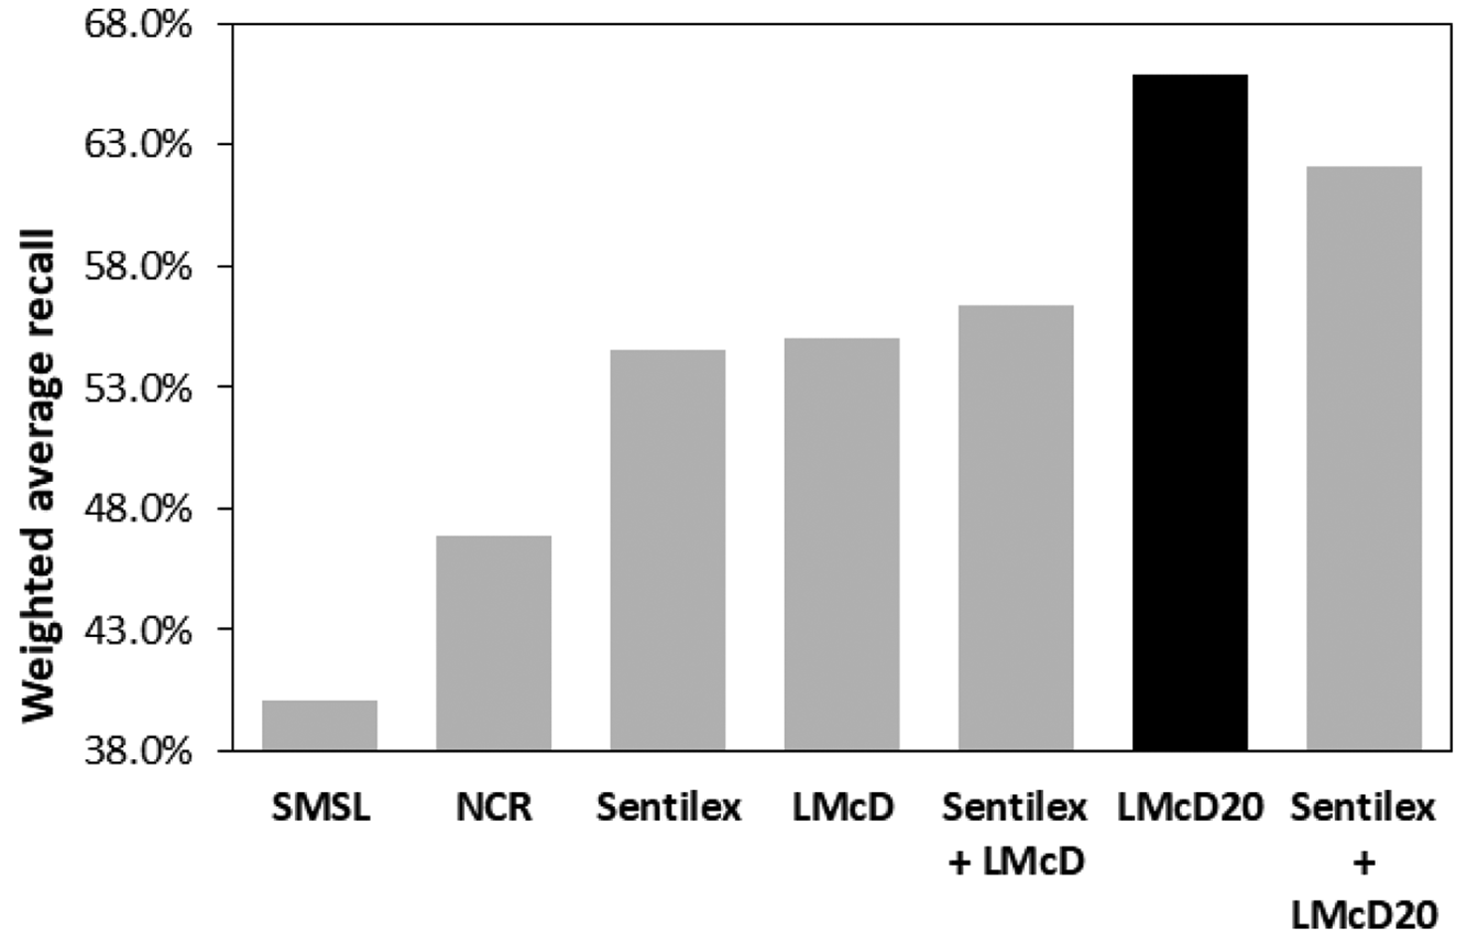
\includegraphics[width=0.85\linewidth]{gfx/m4l3_taborda_fig2_comparing_lexicons_war.png}
\par\smallskip{\small \textbf{Hình 2:} So sánh các từ điển cảm xúc, độ nhạy trung bình có trọng số (WAR).}
\end{figure}

Trong nỗ lực cải thiện WAR tổng thể, LMcD20 đã được tạo ra như đã mô tả trước đó ở mục 5.1. Đáng chú ý, việc sử dụng độc lập LMcD20 đạt hiệu suất tốt nhất (65.9\%) so với các từ điển còn lại. Cụ thể, LMcD20 cho thấy mức cải thiện 11 p.p. so với LMcD. Có sự sụt giảm về WAR khi kết hợp Sentilex và LMcD20. Sụt giảm này chủ yếu do LMcD20 đặc thù cho các tweet thị trường chứng khoán, còn Sentilex đặc thù cho các đánh giá của khách hàng.

Mặc dù kết quả của LMcD20 có thể được coi là thỏa đáng, một phân tích kỹ lưỡng các kết quả cho thấy rằng một từ điển đơn từ (uni-gram) như LMcD20 vẫn còn hạn chế trong việc phân loại cảm xúc tweet. Do đó, chúng tôi nhận thấy cần phải kết hợp một GSA với từ điển đặc thù lĩnh vực này, điều đã được thực hiện thông qua việc triển khai SA-MAIS như mô tả ở mục 6.

\section{6. SA-MAIS: phương pháp lai để phân tích tweet thị trường chứng khoán}

Mục này trình bày chi tiết việc triển khai SA-MAIS. Mục 6.1 mô tả cách kết hợp GSA và các từ điển đặc thù lĩnh vực, còn mục 6.2 làm nổi bật các kết quả đạt được với việc triển khai này.

\subsection*{6.1. Phân loại tweet}

Để đạt được hiệu suất tốt nhất, SA-MAIS kết hợp một bộ phân loại cảm xúc tổng quát, chẳng hạn như thư viện TextBlob, bộ công cụ Stanza, VADER, BERTweet, Twitter-roBERTa, FinBERT, và một từ điển đặc thù lĩnh vực (như SMSL, NRC, Sentilex, LMcD hoặc từ điển LMcD20 đã được tăng cường). Kỹ thuật này dựa vào việc sử dụng đồng thời cả hai công cụ cho phân tích văn bản và tích hợp kết quả phân loại bằng một tổ hợp lồi (convex combination).

\subsubsection*{6.1.1. Thành phần GSA}

Như đã đề cập trước đó, TextBlob trả về phân cực thể hiện cảm xúc tổng thể của tweet: một giá trị trong khoảng $[-1.0, 1.0]$, với $-1.0$ thể hiện cảm xúc hoàn toàn tiêu cực và $1.0$ là cảm xúc hoàn toàn tích cực. VADER cũng báo cáo phân cực trong cùng khoảng giá trị, nhưng kết quả của Stanza là 0, 1 hoặc 2, lần lượt đại diện cho cảm xúc tiêu cực, trung lập hoặc tích cực. Ba mô hình học sâu dựa trên BERT được sử dụng trong bài báo này, cụ thể là BERTweet, Twitter-roBERTa và FinBERT, đưa ra ba lớp đại diện cho cảm xúc được phân tích trong văn bản. Mặc dù các nhãn được biểu diễn khác nhau như đã đề cập trước đó, tất cả các mô hình đều có xu hướng biểu diễn cảm xúc tích cực, tiêu cực và trung lập.

Điều này có nghĩa là, bất kể công cụ nào được sử dụng, giá trị phân cực cảm xúc do thành phần GSA của SA-MAIS đưa ra là một giá trị $P_0 \in [-1.0, 1.0]$. Do đó, trong khi giá trị trả về ($pol$) từ các bộ phân tích cảm xúc tổng quát TextBlob và VADER được lấy theo giá trị thực của chúng, trong trường hợp sử dụng Stanza, đầu ra của nó được chuyển đổi thành $-1$, $0$ hoặc $1$, lần lượt biểu thị cảm xúc tiêu cực, trung lập hoặc tích cực. Tương tự phép chuyển đổi của Stanza, đầu ra của BERTweet, Twitter-roBERTa và FinBERT được chuyển đổi thành $-1$, $0$ hoặc $1$, lần lượt biểu thị cảm xúc tiêu cực, trung lập hoặc tích cực. Phương trình (2) định nghĩa giá trị phân cực GSA cho SA-MAIS, trong đó $pol$ đại diện cho cảm xúc do một GSA cụ thể đưa ra và các biến thể BERT đại diện cho các mô hình được sử dụng trong nghiên cứu này (BERTweet, Twitter-roBERTa và FinBERT):

\[
P_0 =
\begin{cases}
pol - 1, & \text{nếu } pol \text{ là đầu ra của Stanza} \\
-1, & \text{nếu } pol \text{ là tiêu cực từ một mô hình dựa trên BERT} \\
0, & \text{nếu } pol \text{ là trung lập từ một mô hình dựa trên BERT} \\
1, & \text{nếu } pol \text{ là tích cực từ một mô hình dựa trên BERT} \\
pol, & \text{trường hợp còn lại}
\end{cases}
\qquad (2)
\]

\subsubsection*{6.1.2. Thành phần từ điển đặc thù lĩnh vực}

Thành phần đặc thù lĩnh vực của SA-MAIS phân loại từng tweet bằng cách so sánh nội dung của nó với một từ điển đặc thù lĩnh vực ở cấp độ từ. Gọi $W_{\text{pos}}$ là số lượng từ trùng khớp trong tập từ tích cực, và $W_{\text{neg}}$ là số lượng từ trùng khớp trong tập từ tiêu cực. Đầu ra của thành phần này được tính theo phương trình (3):

\[
P_1 =
\begin{cases}
\dfrac{(W_{\text{pos}} - W_{\text{neg}})}{(W_{\text{pos}} + W_{\text{neg}})}, & \text{nếu } (W_{\text{pos}} + W_{\text{neg}}) > 0 \\[2mm]
0, & \text{trường hợp còn lại}
\end{cases}
\qquad (3)
\]

Trong trường hợp không có từ nào của tweet trùng khớp với từ điển đặc thù lĩnh vực, đầu ra của thành phần từ điển đặc thù lĩnh vực bằng 0.

\begin{figure}[H]
\centering
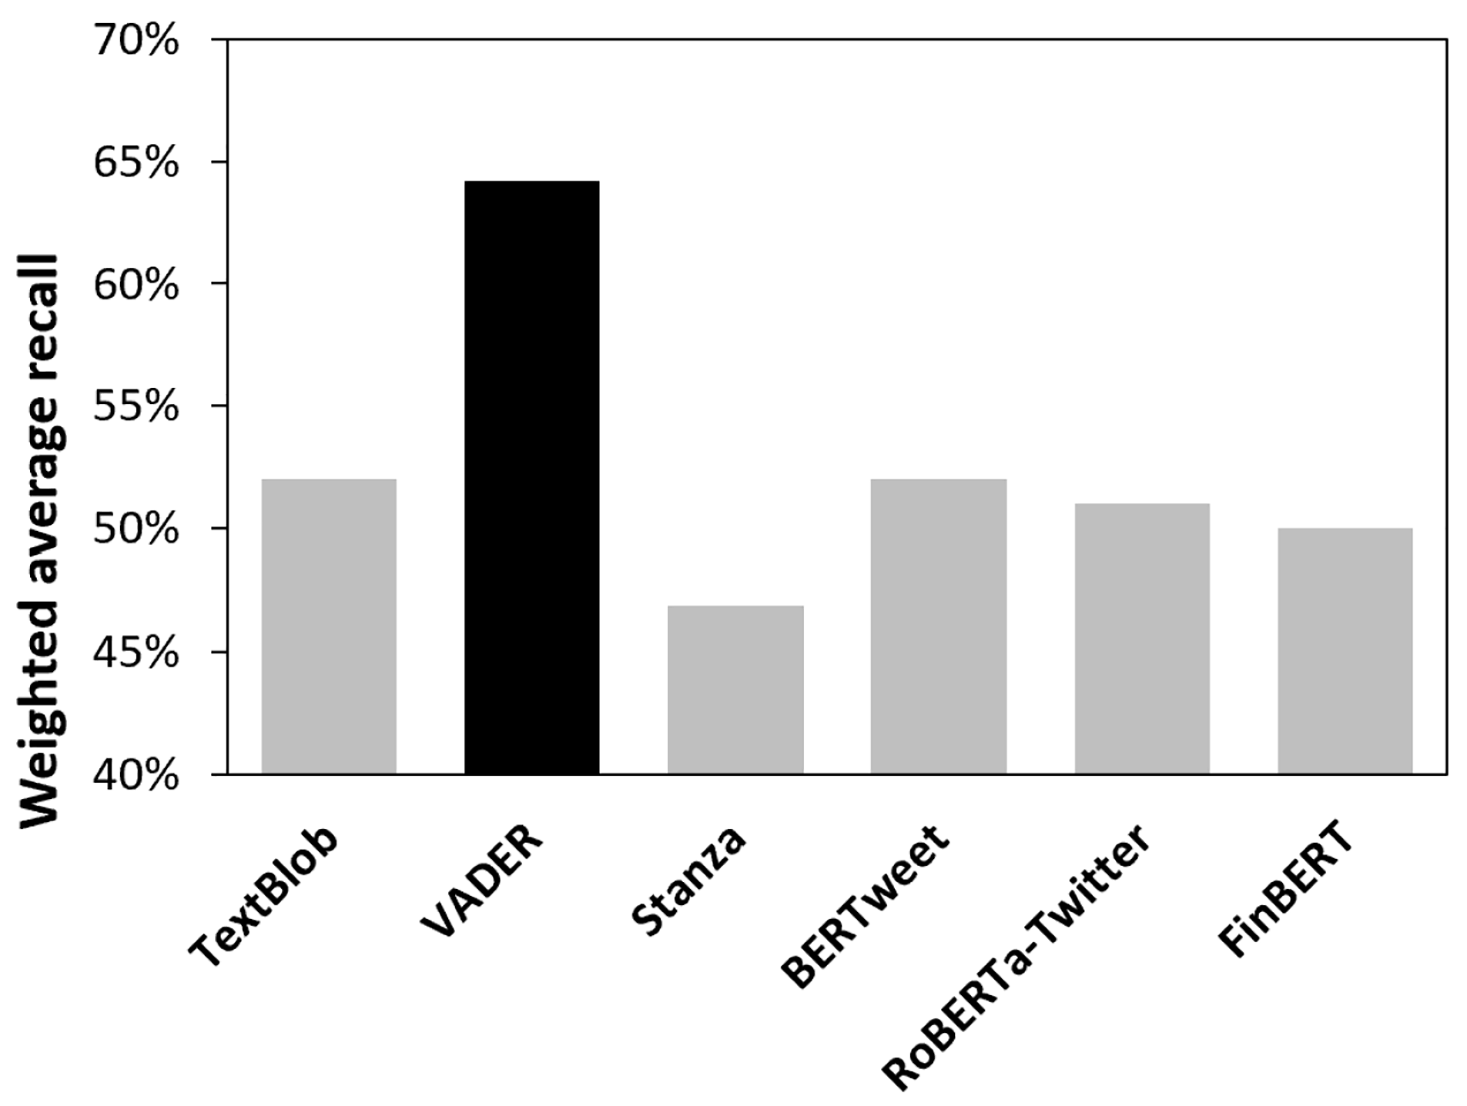
\includegraphics[width=0.75\linewidth]{gfx/m4l3_taborda_fig3_comparing_generalist_sa.png}
\par\smallskip{\small \textbf{Hình 3:} So sánh hiệu suất của các công cụ phân tích cảm xúc tổng quát trên tập dữ liệu của chúng tôi.}
\end{figure}

\subsubsection*{6.1.3. Bộ tích hợp giá trị cảm xúc của SA-MAIS}

Đầu ra của SA-MAIS là một tổ hợp lồi tuyến tính của hai thành phần trước đó, được cho bởi phương trình (4), trong đó $P_0$ là phân cực của GSA, $P_1$ là đầu ra của từ điển đặc thù lĩnh vực, và $\lambda$ là một tham số xác định tầm quan trọng của từ điển đặc thù lĩnh vực trong kết quả cuối cùng. Vì $\lambda \in [0.0, 1.0]$, khoảng giá trị của phân cực không bị thay đổi:

\[
P = (1 - \lambda) \times P_0 + \lambda \times P_1 \qquad (4)
\]

Cuối cùng, phương trình (5) định nghĩa đầu ra dạng phân loại (categorical) của SA-MAIS. Mỗi tweet được phân loại là tiêu cực, trung lập hoặc tích cực, theo giá trị $P$ được cho bởi phương trình (4). Tham số $\beta$ phụ thuộc vào GSA được sử dụng: $\beta = 0.0$ khi sử dụng TextBlob, Stanza, BERTweet, Twitter-roBERTa hoặc FinBERT, và $\beta = 0.05$ khi sử dụng VADER, vì các tác giả của VADER coi một giá trị trong khoảng từ $-0.05$ đến $0.05$ là trung lập:

\[
C =
\begin{cases}
\text{tiêu cực}, & -1.0 \leq P < \beta \\
\text{trung lập}, & -\beta \leq P \leq \beta \\
\text{tích cực}, & \beta < P \leq 1.0
\end{cases}
\qquad (5)
\]

\subsection*{6.2. Kết quả}

Thực nghiệm đầu tiên nhằm thiết lập đường cơ sở (baseline), gồm đánh giá hiệu suất của TextBlob, Stanza, VADER, BERTweet, Twitter-roBERTa và FinBERT khi được sử dụng độc lập trên tập dữ liệu được gán nhãn. Điều này có nghĩa là thực nghiệm được thực hiện bằng cách đặt tham số $\lambda = 0$ trong phương trình (4), và do đó, các từ điển đặc thù lĩnh vực không được sử dụng.

Như thể hiện trong Hình 3, VADER vượt trội rõ rệt so với các công cụ còn lại, đạt WAR xấp xỉ 64.0\% so với 52.0\% của BERTweet, mô hình đạt WAR cao nhất trong số các mô hình còn lại được so sánh. Như vậy, trong số các công cụ được so sánh, VADER nổi bật là bộ phân loại phù hợp nhất cho phân tích cảm xúc tweet thị trường chứng khoán.

So sánh các ma trận nhầm lẫn (confusion matrices) phân loại của TextBlob và VADER (Bảng 4 và Bảng 5), có thể thấy rằng TextBlob có tỷ lệ sai sót cao hơn ở lớp cảm xúc tích cực so với khi dự đoán lớp trung lập hoặc lớp tiêu cực. Ngược lại, mặc dù VADER cho thấy một ma trận nhầm lẫn đồng đều hơn, có thể thấy rằng nó chủ yếu sai sót khi phân loại các tweet có cảm xúc tiêu cực. Về ma trận nhầm lẫn của BERTweet (Bảng 6), mô hình này chủ yếu sai sót ở các lớp cảm xúc tích cực và tiêu cực, phân loại nhiều tweet trong số đó là trung lập. Do đó, dường như mô hình này hoặc đang thiếu ngữ cảnh hoặc thiếu các từ có phân cực đặc thù lĩnh vực để đạt được phân loại phù hợp cho các tweet tài chính liên quan đến thị trường chứng khoán.

\begin{figure}[H]
\centering
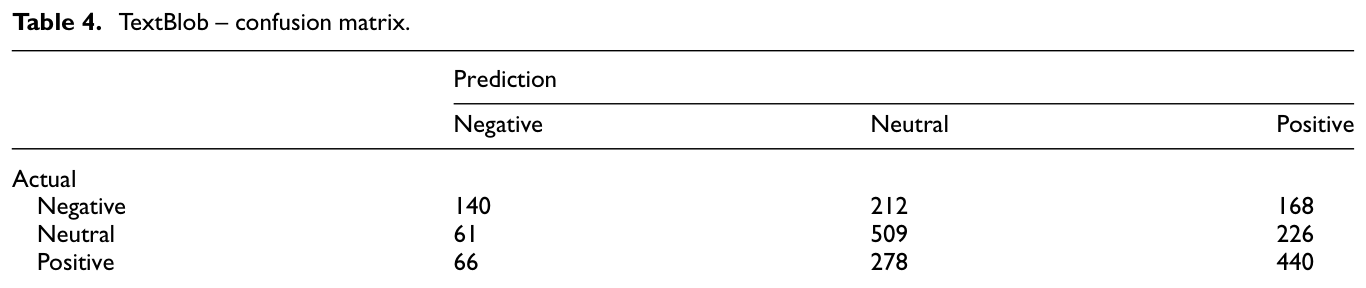
\includegraphics[width=0.85\linewidth]{gfx/m4l3_taborda_table4_textblob_confusion.png}
\par\smallskip{\small \textbf{Bảng 4:} Ma trận nhầm lẫn của TextBlob.}
\end{figure}

\begin{figure}[H]
\centering
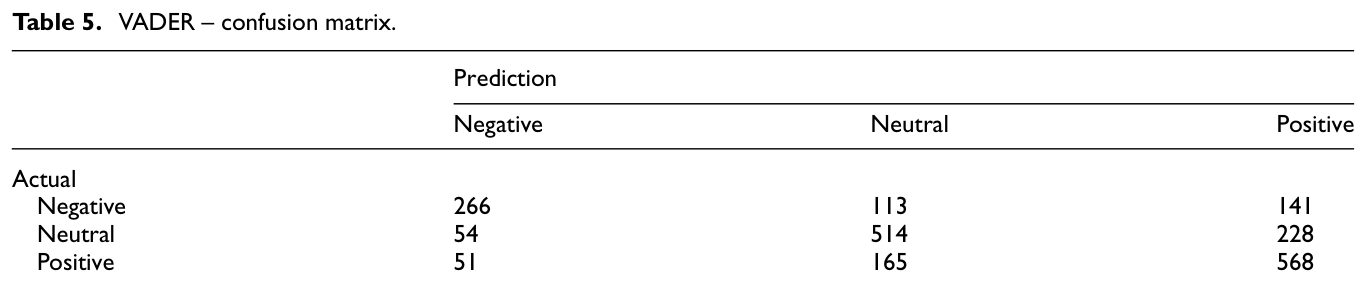
\includegraphics[width=0.85\linewidth]{gfx/m4l3_taborda_table5_vader_confusion.png}
\par\smallskip{\small \textbf{Bảng 5:} Ma trận nhầm lẫn của VADER.}
\end{figure}

\begin{figure}[H]
\centering
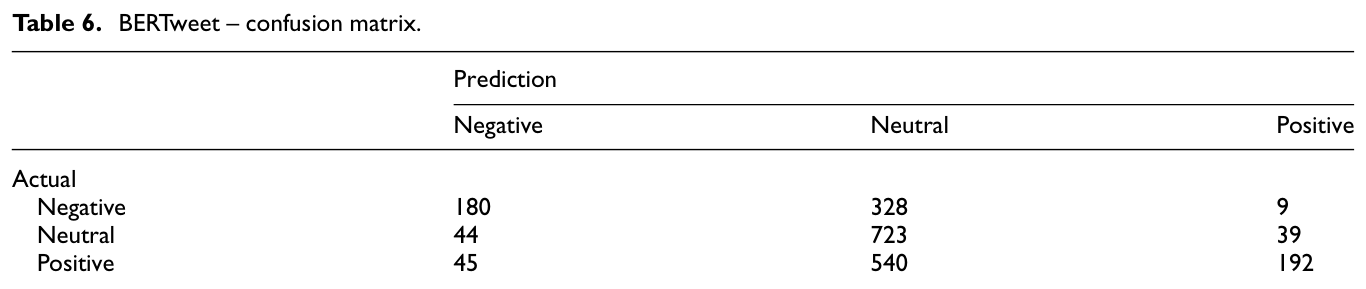
\includegraphics[width=0.85\linewidth]{gfx/m4l3_taborda_table6_bertweet_confusion.png}
\par\smallskip{\small \textbf{Bảng 6:} Ma trận nhầm lẫn của BERTweet.}
\end{figure}

Với các kết quả trên, cách tiếp cận tích hợp của SA-MAIS được đánh giá bằng cách sử dụng VADER làm thành phần tổng quát kết hợp với LMcD20, từ điển đạt kết quả tốt nhất trong các thực nghiệm ở mục 5.2.

Như có thể quan sát trong Hình 4, WAR của việc phân loại cảm xúc đã tăng từ 65.9\% với LMcD20 và 64.0\% với VADER lên đến 71.8\% với VADER + LMcD20. Như vậy, có một mức tăng tổng thể 6 p.p. so với LMcD20 sử dụng độc lập và 8 p.p. so với VADER sử dụng độc lập. Lưu ý rằng kết quả tốt nhất đạt được tại $\lambda = 0.5$, nghĩa là cả hai thành phần có tỷ trọng đóng góp bằng nhau vào việc phân loại cảm xúc cuối cùng của tweet.

\begin{figure}[H]
\centering
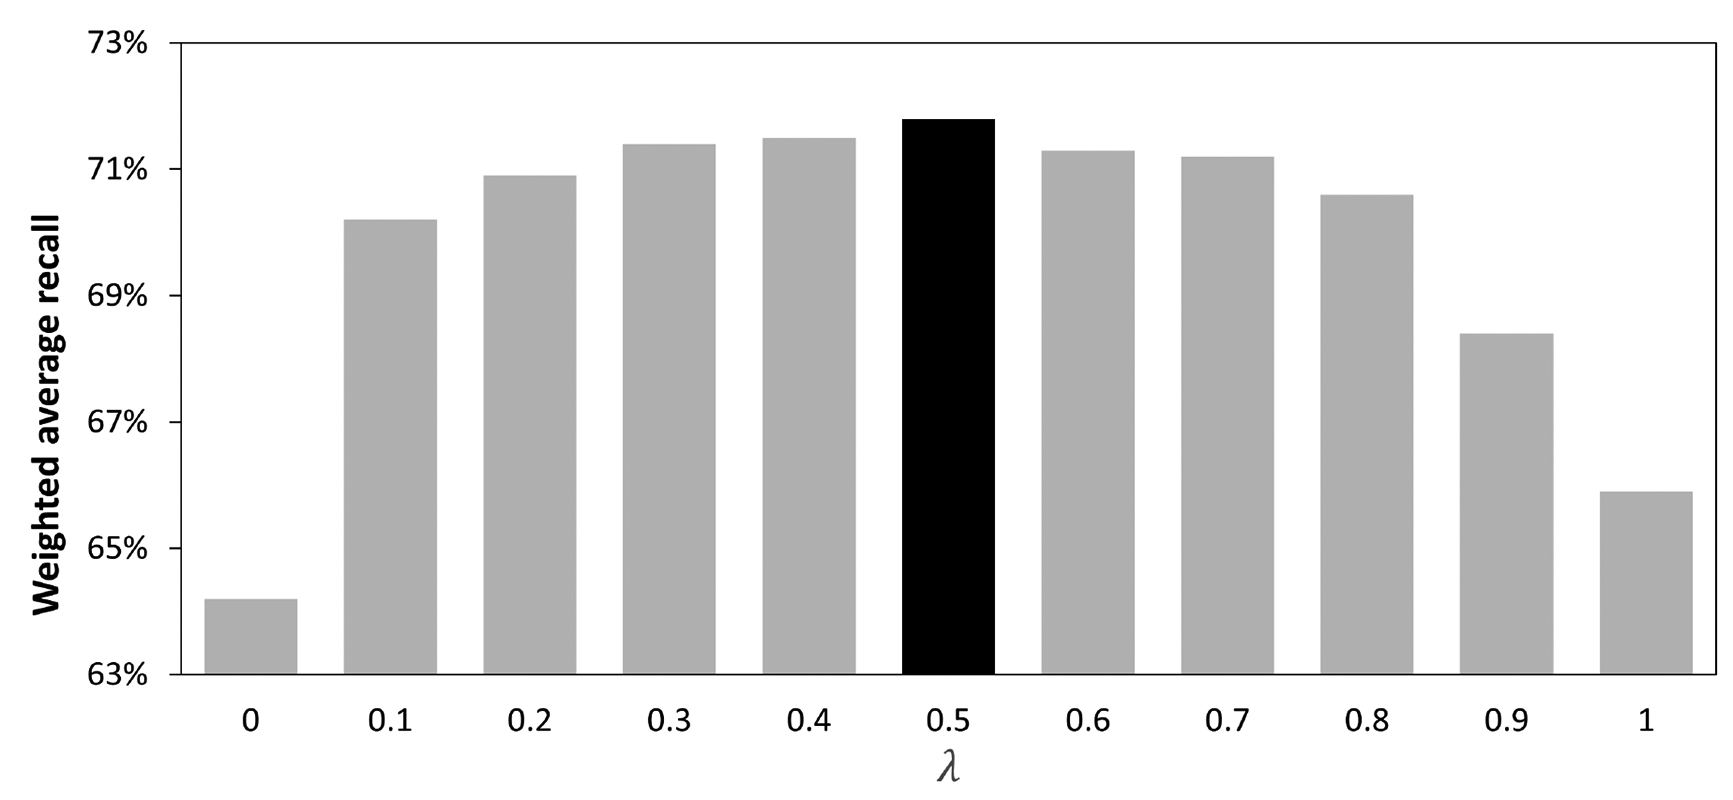
\includegraphics[width=0.75\linewidth]{gfx/m4l3_taborda_fig4_lmcd20_vader_lambda.png}
\par\smallskip{\small \textbf{Hình 4:} So sánh hiệu suất của LMcD20 và VADER theo các giá trị khác nhau của $\lambda$.}
\end{figure}

Các giá trị thước đo tổng thể cho SA-MAIS khi sử dụng VADER cộng với LMcD20 với $\lambda = 0.5$ được trình bày trong Bảng 7, cho biết chi tiết hành vi của SA-MAIS đối với từng lớp cảm xúc bằng cách hiển thị các thước đo đánh giá phổ biến nhất (precision, recall và F1-score). Về recall, số liệu thống kê cho thấy phân loại hiệu quả nhất là dành cho lớp tích cực, với giá trị 87.1\%. Lớp cảm xúc tiêu cực cho giá trị recall 71.4\%, còn lớp trung lập có giá trị recall thấp nhất là 57.8\%. Giá trị precision thấp nhất, 64.6\%, đạt được ở lớp tích cực, trong khi lớp trung lập là lớp có precision cao nhất, đạt 82.9\%. Theo các kết quả trên, các lớp có F1-score tốt nhất là lớp tích cực và lớp tiêu cực, lần lượt đạt 74.2\% và 73.6\%. Nhìn chung, F1-score trung bình có trọng số của SA-MAIS là 71.7\%.

\begin{figure}[H]
\centering
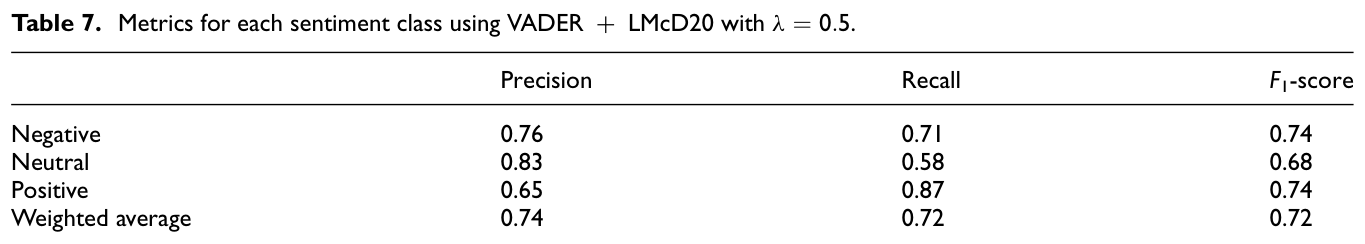
\includegraphics[width=0.6\linewidth]{gfx/m4l3_taborda_table7_metrics_vader_lmcd20.png}
\par\smallskip{\small \textbf{Bảng 7:} Các thước đo cho từng lớp cảm xúc khi sử dụng VADER + LMcD20 với $\lambda = 0.5$.}
\end{figure}

Để minh họa rõ hơn thế nào là một tweet tích cực, trung lập và tiêu cực, Bảng 8 trình bày một ví dụ về dự đoán đúng của SA-MAIS cho từng lớp cảm xúc này.

\begin{figure}[H]
\centering
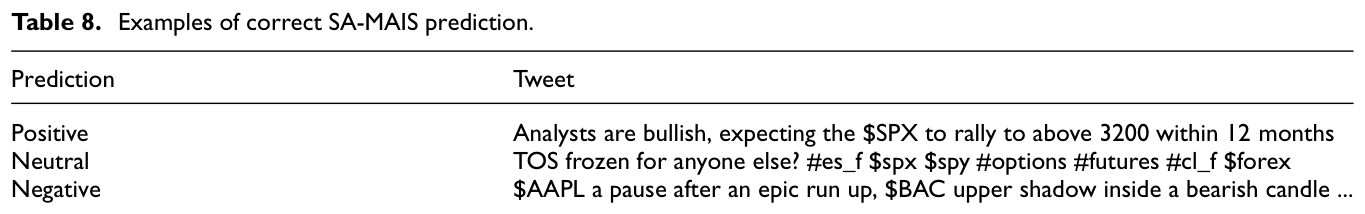
\includegraphics[width=0.9\linewidth]{gfx/m4l3_taborda_table8_correct_prediction_examples.png}
\par\smallskip{\small \textbf{Bảng 8:} Ví dụ về các dự đoán đúng của SA-MAIS.}
\end{figure}

\section{7. Đóng góp và hàm ý thực tiễn}

Nghiên cứu này đề xuất một phương pháp tham số lai (hybrid parametric approach) để phân tích phân cực cảm xúc của các thông điệp văn bản ngắn, kết hợp một bộ phân tích cảm xúc tổng quát với một từ điển đặc thù lĩnh vực đã được cập nhật, gọi là SA-MAIS.

Nghiên cứu cung cấp những hiểu biết mới về phân tích cảm xúc đặc thù lĩnh vực đối với văn bản ngắn trên mạng xã hội. Nó mô tả một cách tiếp cận phương pháp luận mới và cho thấy rằng (a) một cách đơn giản nhưng hiệu quả để tích hợp vốn từ vựng cập nhật theo thời gian từ văn bản ngắn đặc thù lĩnh vực mang lại giá trị gia tăng cho các nhiệm vụ phân loại, và (b) việc sử dụng từ điển đã được tăng cường này cải thiện các công cụ phân tích cảm xúc tổng quát hiện có, cung cấp một công cụ chính xác hơn để phân tích cảm xúc văn bản trong một ngôn ngữ chuyên biệt kỹ thuật cụ thể. Cụ thể, chúng tôi mô tả một bằng chứng khái niệm của phương pháp luận này bằng cách áp dụng nó vào việc phân tích và dự đoán tweet thị trường chứng khoán. Mặc dù trọng tâm của nghiên cứu này là thị trường chứng khoán, cách tiếp cận tổng quát có thể được áp dụng cho các lĩnh vực khác nhau, dù là tài chính hay không, bằng cách thay thế từ điển đặc thù và sử dụng các tweet từ lĩnh vực được chọn để tăng cường từ điển mới.

Thứ hai, nghiên cứu đóng góp cho lĩnh vực học máy và khai phá văn bản (text mining) bằng cách cung cấp một kho ngữ liệu thị trường chứng khoán mới được gán nhãn để làm chuẩn so sánh cho các phương pháp và kỹ thuật mới. Thứ ba, bằng cách so sánh hiệu suất của một số công cụ tổng quát hiện có, nghiên cứu cho thấy rằng các công cụ này, khi sử dụng độc lập, phần lớn không đủ để phân loại chính xác và chi tiết cảm xúc của các tweet liên quan đến thị trường chứng khoán.

\section{8. Kết luận}

Một phương pháp phân tích cảm xúc mới, SA-MAIS, sử dụng một khung dựa trên việc tích hợp có kiểm soát một GSA và một từ điển đặc thù lĩnh vực đã được trình bày. Hệ thống này kết hợp GSA nổi tiếng VADER với một từ điển đặc thù lĩnh vực, LMcD20, được cập nhật với các xu hướng từ vựng gần đây hơn. Một phiên bản được tăng cường của từ điển tài chính LMcD, có tên LMcD20, tích hợp các từ mới hơn và cập nhật liên quan đến tài chính, được tự động rút trích từ các tweet thị trường chứng khoán, cũng đã được trình bày.

Phương pháp kết hợp lai của SA-MAIS giữa phân tích tổng quát và đặc thù lĩnh vực đã được kiểm định toàn diện bằng cách sử dụng sáu GSA phổ biến: TextBlob, Stanza [8], VADER [9] và các mô hình tiên tiến được huấn luyện chuyên biệt BERTweet [41], Twitter-roBERTa và FinBERT [42], cùng với bốn từ điển tài chính chuyên biệt hiện có: từ điển cảm xúc tài chính LMcD [10], SMSL [11], Sentilex [24] và NRC [53]. Là một bằng chứng khái niệm, sau khi thực hiện một số thực nghiệm, có thể kết luận rằng từ điển mới được tăng cường LMcD20 cho thấy mức tăng khoảng sáu điểm phần trăm về kết quả WAR đối với kho ngữ liệu Twitter thị trường chứng khoán. Hơn nữa, việc triển khai SA-MAIS bằng cách tích hợp VADER với LMcD20 đã cải thiện các kết quả trước đó trên tất cả các lớp phân loại có thể, tích cực, tiêu cực và trung lập. Những kết quả này cho thấy SA-MAIS có thể được sử dụng như một công cụ trong các hệ thống phức tạp hơn để dự đoán diễn biến thị trường, vì nó vượt trội hơn các mô hình NLP tiên tiến nhất sử dụng học sâu.

Cuối cùng, tất cả các thực nghiệm được tiến hành sử dụng một kho ngữ liệu mới được gán nhãn, công bố công khai tại \url{https://github.com/taborda11/SAMAIS}. Về các hướng nghiên cứu tiếp theo, nghiên cứu này tất yếu vẫn còn một số hạn chế. Lý tưởng nhất, tập dữ liệu gồm 2100 tài liệu được gán nhãn nên được mở rộng, vì việc gán nhãn thủ công thêm các tweet không chỉ giúp làm giàu kho ngữ liệu đã gán nhãn mà còn là một tài sản quan trọng cho việc tăng cường LMcD20 trong tương lai, từ đó cải thiện kết quả phân loại cảm xúc của SA-MAIS. Thứ hai, các từ điển phức tạp hoặc có mục đích hơn, có thể đại diện cho các mối quan hệ giữa các từ và thêm thông tin ngôn ngữ, có thể đóng vai trò then chốt trong việc cải thiện các kết quả được trình bày ở đây. Thứ ba, các thử nghiệm trực tuyến (online tests) với SA-MAIS có thể cải thiện hiệu suất của công cụ này và mở rộng phạm vi ứng dụng.

\section*{Tuyên bố xung đột lợi ích}

Các tác giả tuyên bố không có xung đột lợi ích tiềm ẩn nào liên quan đến việc nghiên cứu, viết bài và/hoặc xuất bản bài báo này.

\section*{Tài trợ}

Các tác giả công bố đã nhận được hỗ trợ tài chính sau đây cho việc nghiên cứu, viết bài và/hoặc xuất bản bài báo này: Nghiên cứu này được tài trợ một phần bởi nguồn ngân sách quốc gia thông qua Fundação para a Ciência e a Tecnologia (FCT) với các mã số tham chiếu UIDB/50021/2020 và UIDB/00315/2020.

\section*{Ghi chú}

\begin{enumerate}
  \item https://github.com/taborda11/SAMAIS.
  \item https://ieee-dataport.org/open-access/stock-market-tweets-data.
  \item https://stocktwits.com.
  \item https://textblob.readthedocs.io.
\end{enumerate}

\section*{ORCID iD}

Bruno Taborda \url{https://orcid.org/0000-0002-3564-8662}

% [Đã lược bỏ danh mục Tài liệu tham khảo gốc (tiếng Anh, trích dẫn của tác giả bài gốc) để giảm dung lượng chương; không ảnh hưởng nội dung học thuật chính.]

\chapter{Đọc thêm 2: Dự đoán Biến động Giá Cổ phiếu từ Cảm xúc Nhà đầu tư trên Stocktwits (Liu, Leu \& Holst)}
\label{ch:M4L3DT2}

% Nguồn: Liu, J.-X., Leu, J.-S., & Holst, S. ``Stock price movement prediction based on Stocktwits investor sentiment using FinBERT and ensemble SVM.'' PeerJ Computer Science, 9:e1403, 2023.
% Phần cần đọc: Toàn bộ bài báo
% Nội dung bắt buộc đọc: được kiểm tra trong mọi bài đánh giá (kể cả Quiz).

\section{Thông tin nguồn}

\begin{itemize}
  \item \textbf{Nguồn:} Liu, Jin-Xian, Jenq-Shiou Leu, and Stefan Holst. \emph{Stock price movement prediction based on Stocktwits investor sentiment using FinBERT and ensemble SVM}. PeerJ Computer Science, 9:e1403, 2023. \url{http://doi.org/10.7717/peerj-cs.1403}
  \item \textbf{Phần cần đọc:} Toàn bộ nội dung
\end{itemize}

\section{Tóm tắt}

Cảm xúc nhà đầu tư đóng vai trò then chốt trong thị trường chứng khoán, và trong những năm gần đây, nhiều nghiên cứu đã nỗ lực dự đoán giá cổ phiếu tương lai bằng cách phân tích cảm xúc thị trường thu thập từ mạng xã hội hoặc tin tức. Nghiên cứu này khảo sát việc sử dụng cảm xúc nhà đầu tư từ mạng xã hội, tập trung vào Stocktwits, một nền tảng mạng xã hội dành cho nhà đầu tư. Tuy nhiên, việc dùng cảm xúc nhà đầu tư trên Stocktwits để dự đoán biến động giá cổ phiếu có thể gặp khó khăn do thiếu dữ liệu cảm xúc do người dùng tự gán nhãn và do hạn chế của các bộ phân loại cảm xúc hiện có, vốn có thể phân loại sai các bình luận trung lập. Để khắc phục những thách thức này, nghiên cứu đề xuất một cách tiếp cận thay thế sử dụng FinBERT, một mô hình ngôn ngữ đã được huấn luyện trước, được thiết kế chuyên biệt để phân tích cảm xúc văn bản tài chính. Nghiên cứu này đề xuất một máy vector hỗ trợ tập hợp (ensemble support vector machine, SVM) nhằm cải thiện độ chính xác của dự đoán biến động giá cổ phiếu. Sau đó, mô hình dự đoán biến động giá tương lai của Quỹ hoán đổi danh mục (Exchange Traded Fund) chỉ số SPDR S\&P 500, sử dụng phương pháp cửa sổ trượt (rolling window) để tránh thiên lệch nhìn trước (look-ahead bias). Thông qua việc so sánh các kỹ thuật khác nhau để tạo ra cảm xúc, kết quả của chúng tôi cho thấy việc sử dụng mô hình FinBERT để phân tích cảm xúc mang lại kết quả tốt nhất, với điểm F1 (F1-score) cao hơn 4 đến 5\% so với các kỹ thuật khác. Ngoài ra, máy vector hỗ trợ tập hợp được đề xuất cải thiện độ chính xác của dự đoán biến động giá cổ phiếu so với máy vector hỗ trợ nguyên bản trong một loạt các thực nghiệm.

\textbf{Chủ đề:} Trí tuệ nhân tạo, Khai phá dữ liệu và Học máy, Khoa học Dữ liệu, Khai phá Văn bản, Phân tích Cảm xúc

\textbf{Từ khóa:} Phân tích cảm xúc, Stocktwits, Dự đoán giá cổ phiếu, Học máy, SVM, SPY, FinBERT, Tài chính

\section{Giới thiệu}

Theo giả thuyết thị trường hiệu quả (efficient market hypothesis, EMH) (Fama, 1970), thị trường chứng khoán được coi là hiệu quả vì người ta giả định rằng tất cả thông tin sẵn có đã được phản ánh vào giá cổ phiếu. Nếu giả định EMH là đúng, thì giả thuyết bước đi ngẫu nhiên (random walk hypothesis) (Fama, 1965) cho rằng tin tức tương lai là ngẫu nhiên và nhà đầu tư không thể sử dụng kiến thức trước đó của mình để tạo ra lợi nhuận vượt trội. Tuy nhiên, nhiều nghiên cứu được thực hiện trong vài thập kỷ qua đã cho thấy rằng việc dự đoán giá thị trường tương lai là khả thi thông qua các kỹ thuật như phân tích cơ bản, phân tích kỹ thuật và phân tích cảm xúc. Trong số đó, dự đoán giá cổ phiếu dựa trên cảm xúc liên quan đến việc phân tích tin tức, bài viết đã xuất bản và dữ liệu mạng xã hội để dự đoán giá cổ phiếu tương lai (Nousi \& Tjortjis, 2021). Trong những năm gần đây, ngày càng nhiều nhà đầu tư chia sẻ quan điểm thị trường của họ trên mạng xã hội. Do đó, trong nghiên cứu này, chúng tôi hướng đến việc thu thập ý kiến nhà đầu tư từ một trang mạng xã hội dành cho nhà đầu tư, Stocktwits (\url{https://Stocktwits.com/}), kết hợp chúng với dữ liệu lịch sử cổ phiếu, và sử dụng một mô hình học máy để dự đoán biến động giá cổ phiếu tương lai.

Stocktwits (\url{https://Stocktwits.com/}) là một cộng đồng trực tuyến phổ biến dành cho nhà đầu tư và nhà giao dịch, tương tự Twitter. Được thành lập năm 2008, trang web cho phép người dùng thảo luận về các cổ phiếu cụ thể và chia sẻ quan điểm của họ về triển vọng tương lai. Thông qua các cuộc trao đổi với nhà đầu tư khác và nhà giao dịch chuyên nghiệp, người dùng có thể phân tích thị trường và đưa ra các quyết định đầu tư sáng suốt. Hình 1 cho thấy người dùng có thể cung cấp bình luận về một cổ phiếu nhất định, và ở góc dưới bên phải cho phép người dùng gán cảm xúc tăng giá (bullish) hoặc giảm giá (bearish), hoặc không gán cảm xúc nào.

\begin{figure}[H]
\centering
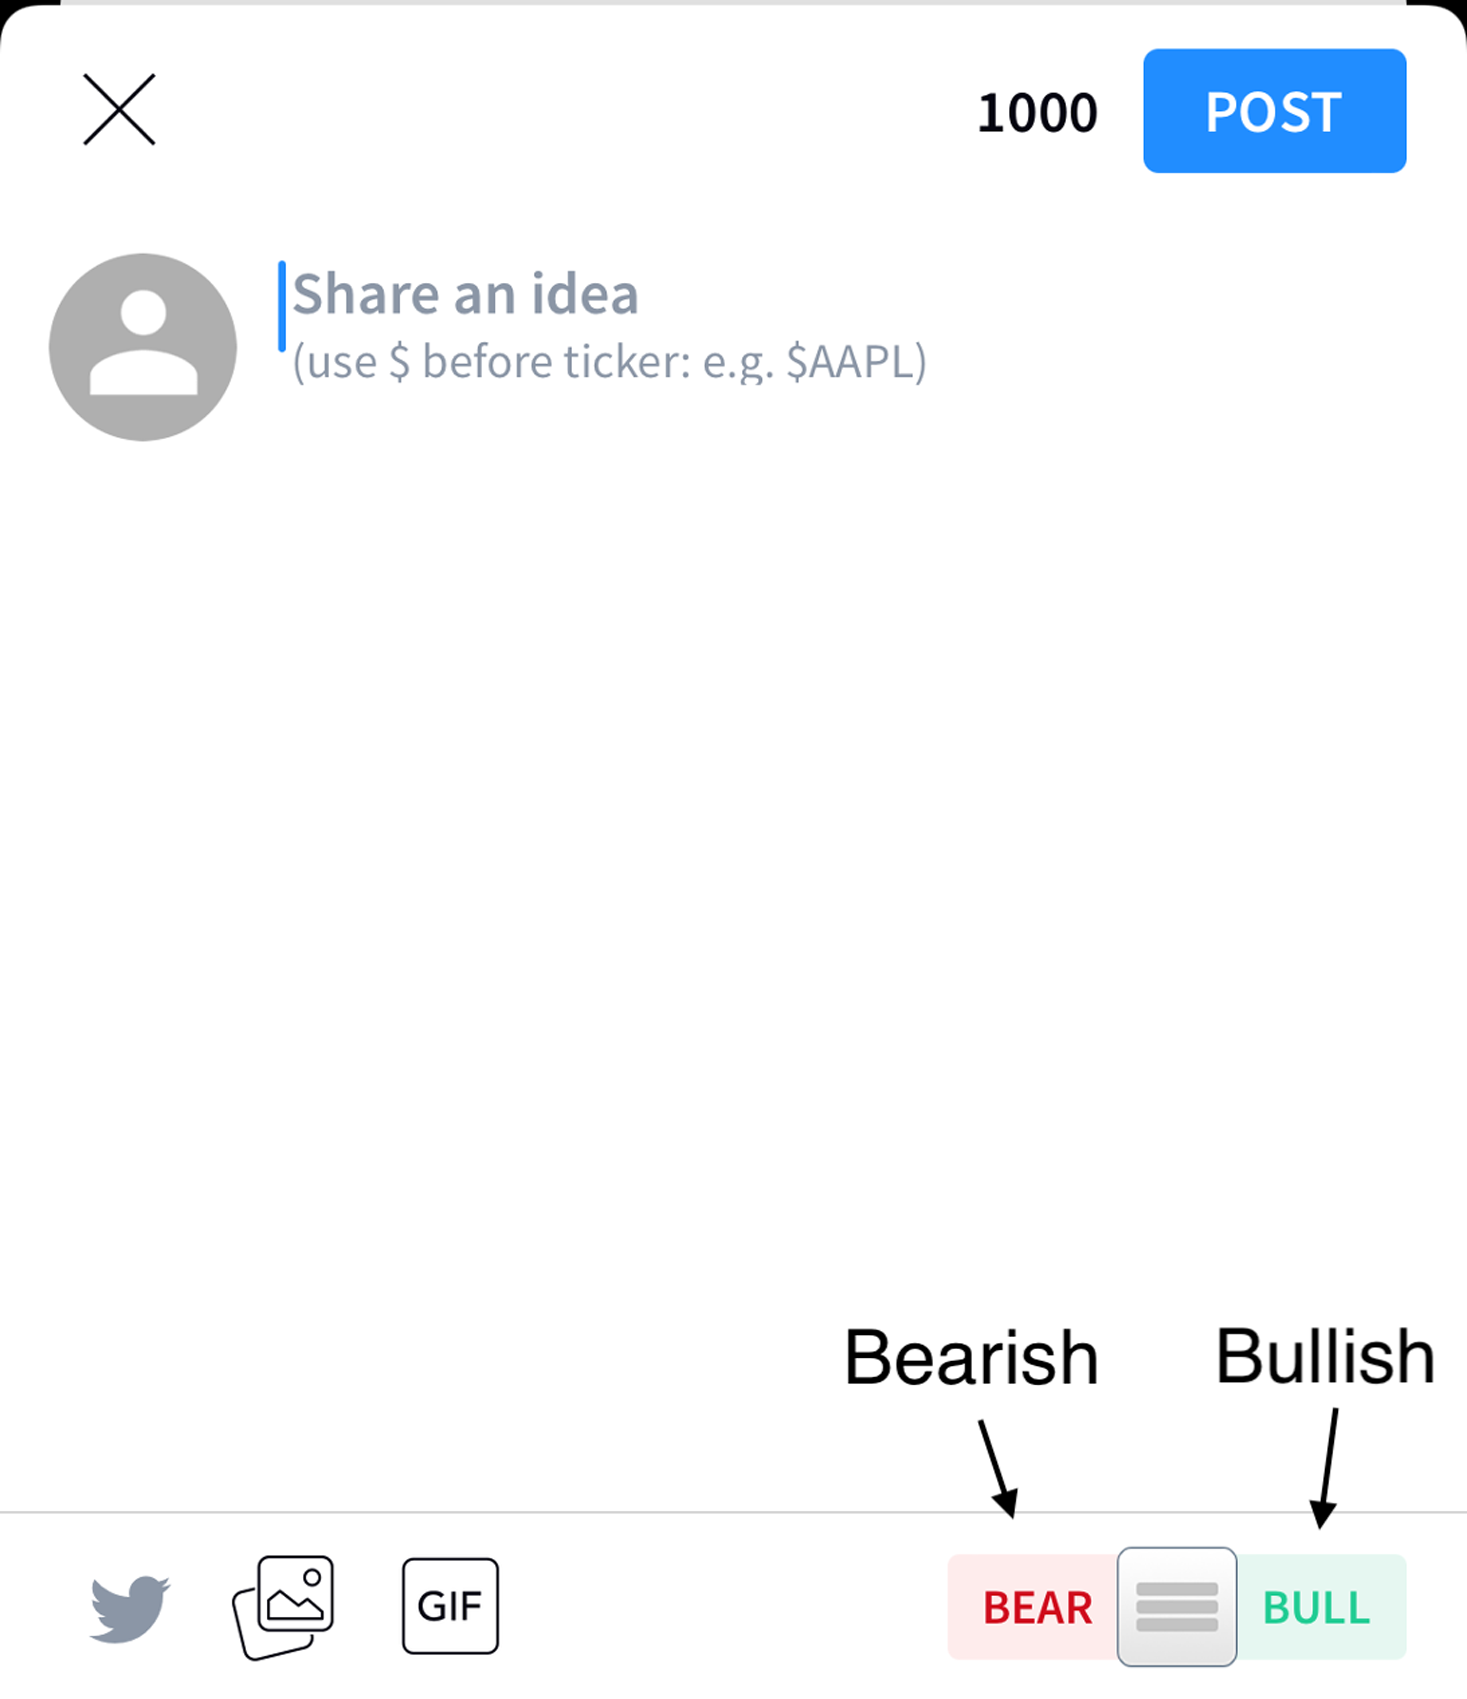
\includegraphics[width=0.6\linewidth]{gfx/m4l3_liu_fig1_stocktwits_ui.png}
\par\smallskip{\small \textbf{Hình 1:} Giao diện người dùng cho việc đăng bình luận và cảm xúc về các cổ phiếu cụ thể.}
\end{figure}

Trên Stocktwits, người dùng có tùy chọn gán nhãn bình luận của họ là tăng giá hoặc giảm giá, hoặc không gán nhãn. Điều này khiến việc dự đoán biến động cổ phiếu bằng cách phân tích cảm xúc trên Stocktwits trở nên khó khăn. Có nhiều cách tiếp cận để thu thập cảm xúc nhà đầu tư. Cách tiếp cận đơn giản nhất là (1) chỉ thu thập cảm xúc từ các bình luận đã được người dùng gán nhãn. Lý do là người dùng chủ động gán nhãn cảm xúc nên rủi ro phân loại sai giảm đi. Nhược điểm chính là dữ liệu cảm xúc có thể không đủ, dẫn đến chỉ số cảm xúc nhà đầu tư được tính toán không phản ánh đầy đủ cảm xúc thị trường. Do đó, hầu hết các nghiên cứu sử dụng một trong hai phương pháp sau: (2) sử dụng các bộ phân loại cảm xúc đa mục đích như VADER (Hutto \& Gilbert, 2014) hoặc Textblob (\url{https://textblob.readthedocs.io/en/dev/}) để phân tích tất cả bình luận (Koukaras, Nousi \& Tjortjis, 2022); (3) sử dụng tất cả các bình luận đã được người dùng gán nhãn trên Stocktwits để xây dựng một bộ phân loại cảm xúc và gán nhãn bình luận nhằm tăng lượng dữ liệu cảm xúc (Gupta \& Chen, 2020). Tuy nhiên, kết quả phân loại cảm xúc sẽ không hoàn toàn chính xác nếu dùng một mô hình phân loại cảm xúc để gán nhãn bình luận. Do đó, cần xem xét liệu có nên sử dụng một bộ phân loại cảm xúc trong việc dự đoán biến động giá cổ phiếu tương lai hay không.

Do thực tế là Stocktwits chỉ cho phép người dùng cung cấp nhãn cảm xúc tăng giá và giảm giá, điều này có thể dẫn đến việc tính toán không chính xác chỉ số cảm xúc cho các mô hình phân tích cảm xúc hai lớp. Điều này sẽ ảnh hưởng tiêu cực đến độ chính xác của dự đoán cổ phiếu. Để cải thiện độ chính xác của chỉ số cảm xúc cho dự đoán biến động giá cổ phiếu, chúng tôi đề xuất một cách tiếp cận mới lạ: sử dụng FinBERT (Araci, 2019), một mô hình phân tích cảm xúc tiên tiến nhất (state-of-the-art) trong lĩnh vực tài chính, để phân loại bình luận trên Stocktwits thành tích cực, tiêu cực, hoặc trung lập. Cách này có thể giảm đáng kể nhiễu, nhờ đó khắc phục một số hạn chế của việc sử dụng bộ phân loại cảm xúc hai lớp trên bình luận Stocktwits. Trong khi FinBERT thường được sử dụng để phân tích bài viết, tin tức và báo cáo tài chính, các nguồn dữ liệu này bị hạn chế và khó cung cấp dữ liệu thời gian thực với khối lượng lớn như mạng xã hội, điều thiết yếu để đạt được độ chính xác dự đoán lý tưởng. Do đó, chúng tôi áp dụng FinBERT để phân loại bình luận trên Stocktwits nhằm nâng cao mức độ hiểu biết vĩ mô của nó, nắm bắt cảm xúc tổng thể của một số lượng lớn nhà đầu tư và quan điểm của họ về các cổ phiếu cụ thể trên mạng xã hội.

Như đã đề cập, bộ phân loại cảm xúc được sử dụng trong nghiên cứu này là FinBERT. Sau khi phân loại cảm xúc, mục tiêu của chúng tôi là dự đoán biến động giá cổ phiếu tương lai. Trong các nghiên cứu trước đây, máy vector hỗ trợ (support vector machines, SVM) (Cortes \& Vapnik, 1995) đã được sử dụng để dự đoán giá cổ phiếu với kết quả xuất sắc (Tripathy, 2019). Hơn nữa, để nâng cao độ chính xác của dự đoán biến động giá cổ phiếu, chúng tôi đề xuất một mô hình mới lạ kết hợp kỹ thuật bagging (Breiman, 1996) với máy vector hỗ trợ. Ít nghiên cứu trong quá khứ đã đề cập đến việc kết hợp hai kỹ thuật này. Trong nghiên cứu này, chúng tôi so sánh hiệu suất của chúng thông qua năm thực nghiệm.

Ngoài ra, hầu hết các nghiên cứu hiện có dự đoán biến động giá giữa giá đóng cửa và giá mở cửa. Tuy nhiên, điều này không mang lại sự linh hoạt cho nhà đầu tư cần đưa ra quyết định giao dịch tức thì hoặc trong cùng ngày. Do đó, chúng tôi thu thập giá cổ phiếu trong phiên (intraday) để dự đoán biến động giá so với giá mở cửa.

Dựa trên những điều trên, các đóng góp chính của nghiên cứu này như sau:
\begin{enumerate}
  \item Chúng tôi thực hiện dự đoán biến động giá cổ phiếu dựa trên cảm xúc sử dụng FinBERT trên một mạng xã hội, Stocktwits, để nâng cao mức độ cảm xúc vĩ mô và cải thiện độ chính xác.
  \item Chúng tôi sử dụng nhiều kỹ thuật khác nhau để thu thập dữ liệu cảm xúc và so sánh hiệu suất của từng kỹ thuật trong việc dự đoán biến động giá cổ phiếu.
  \item Chúng tôi sử dụng máy vector hỗ trợ tập hợp (ensemble support vector machine) để nâng cao độ chính xác của dự đoán biến động giá cổ phiếu.
  \item Chúng tôi thay đổi thời điểm cắt (cut-off time) của dự đoán từ thời điểm đóng cửa sang thời điểm trong phiên (ví dụ: 12:00 giờ miền Đông Hoa Kỳ, EST) để tăng tính linh hoạt trong giao dịch.
\end{enumerate}

Cấu trúc của bài báo này như sau: Mục tiếp theo trình bày tổng quan ngắn gọn về phân tích cảm xúc và mô hình FinBERT, cũng như tổng quan các nghiên cứu gần đây về dự đoán biến động giá cổ phiếu dựa trên cảm xúc. Mục ``Phương pháp luận'' trình bày phương pháp được đề xuất cho dự đoán cổ phiếu, bao gồm thu thập và tiền xử lý dữ liệu, tính toán chỉ số cảm xúc, và máy vector hỗ trợ tập hợp được đề xuất. Mục ``Thiết lập thực nghiệm'' cung cấp tổng quan về chuẩn bị dữ liệu, trích xuất đặc trưng, xây dựng mô hình, và các chỉ số đánh giá. Mục ``Kết quả'' cung cấp chi tiết về từng thực nghiệm và kết quả tương ứng. Mục ``Thảo luận'' so sánh các phát hiện với các nghiên cứu trước đây. Cuối cùng, mục ``Kết luận'' tóm tắt các phát hiện nghiên cứu và vạch ra các định hướng nghiên cứu tương lai.

\section{Công trình liên quan}

Trong mục này, chúng tôi mô tả bối cảnh và các công trình liên quan gần đây trong dự đoán biến động giá cổ phiếu dựa trên cảm xúc. Điều này bao gồm các kỹ thuật phân tích cảm xúc, việc sử dụng máy vector hỗ trợ trong dự đoán giá cổ phiếu, các nghiên cứu liên quan gần đây, và mô hình FinBERT.

\subsection*{Các kỹ thuật phân tích cảm xúc}

Phân tích cảm xúc (sentiment analysis) là một lĩnh vực con của xử lý ngôn ngữ tự nhiên (natural language processing, NLP) có thể suy luận cảm xúc hoặc quan điểm của một cụm từ hoặc văn bản và phân loại nó là tích cực, tiêu cực, trung lập, v.v. (Sidogi, Mbuvha \& Marwala, 2021). Một trong những nguồn thu thập bình luận từ mọi người là mạng xã hội, và trong những năm gần đây, đã có nhiều nghiên cứu sử dụng những hiểu biết sâu sắc từ bình luận mạng xã hội để giải quyết nhiều vấn đề khác nhau. Shamoi và cộng sự (2022) đã sử dụng các bài đăng trên Twitter để tìm hiểu nhận thức của công chúng về chế độ ăn dựa trên thực vật và áp dụng các kỹ thuật phân tích cảm xúc để xác định liệu cảm xúc trong văn bản là tích cực hay tiêu cực. Những phát hiện này có thể giúp các chuyên gia y tế xây dựng các kế hoạch sức khỏe phù hợp và khuyến khích nhiều người hơn duy trì chế độ ăn dựa trên thực vật lành mạnh. Ko \& Chang (2021) đã thực hiện phân tích cảm xúc trên các bài đăng từ nền tảng PPT và sử dụng mô hình bộ nhớ ngắn hạn dài (long short-term memory, LSTM) để dự đoán giá cổ phiếu. Tuy nhiên, do bản chất phổ biến rộng rãi của mạng xã hội, có khả năng xảy ra các cuộc tấn công cá nhân hoặc phân biệt đối xử dựa trên chủng tộc và giới tính trên mạng xã hội. Raman và cộng sự (2022) giải thích rằng mặc dù nhiều công ty đã triển khai các thuật toán khác nhau trên nền tảng của họ, vẫn còn khó khăn trong việc phát hiện thường xuyên các bình luận như vậy, và chúng vẫn tiếp tục xuất hiện trên các nền tảng, gây ra tác động tiêu cực đến các nhóm đối tượng bị nhắm đến. Do đó, nghiên cứu đã so sánh các thuật toán phát hiện thù ghét và tấn công khác nhau để phát hiện lời nói mang cảm xúc thù ghét. Vì vậy, phân tích cảm xúc được ứng dụng rộng rãi và mang lại giá trị thương mại đáng kể.

\subsection*{Dự đoán biến động giá cổ phiếu dựa trên cảm xúc sử dụng máy vector hỗ trợ}

Máy vector hỗ trợ (SVM) là một kỹ thuật học có giám sát được giới thiệu bởi Cortes \& Vapnik (1995), có thể được sử dụng để giải quyết các vấn đề liên quan đến cả hồi quy và phân loại. SVM có thể đạt hiệu suất cao trong các nhiệm vụ phân loại, với điều kiện được trang bị hàm nhân (kernel). Khi dữ liệu trong không gian ban đầu không thể được phân tách bằng một bộ phân loại tuyến tính, hàm nhân được dùng để thực hiện phép chiếu phi tuyến, nhằm phân tách dữ liệu trong một không gian có số chiều cao hơn. Do thực tế thị trường chứng khoán là một ví dụ điển hình của hệ thống phi tuyến, động (non-linear, dynamic), SVM thường được sử dụng để dự đoán giá cổ phiếu. Mặc dù SVM hoạt động tốt trong việc giải quyết các bài toán phân loại, nó vẫn có một số nhược điểm. Theo Auria \& Moro (2008), một nhược điểm của SVM là thiếu tính minh bạch của kết quả, khiến việc lấy điểm và xác suất phân loại trở nên khó khăn. Hạn chế này có thể cản trở khả năng đưa ra quyết định linh hoạt, đặc biệt khi mua hoặc bán dựa trên xác suất của kết quả phân loại.

Theo phát hiện của Hu, Zhu \& Tse (2013), SVM có khả năng tổng quát hóa tốt cũng như khả năng chống chịu mạnh đối với vấn đề quá khớp (overfitting). Ngược lại, việc huấn luyện một mô hình SVM tương tự như giải một bài toán quy hoạch bậc hai bị ràng buộc tuyến tính, và phân loại SVM luôn tạo ra một nghiệm tối ưu toàn cục duy nhất. Điều này trái ngược với việc huấn luyện một mạng nơ-ron, vốn đòi hỏi tối ưu hóa phi tuyến và có nguy cơ rơi vào nghiệm cực tiểu cục bộ. Ngoài ra, nghiên cứu đó dự đoán giá cổ phiếu bằng cách kết hợp báo cáo thường niên và các yếu tố kinh tế vĩ mô. Các phát hiện cuối cùng chứng minh rằng SVM là một kỹ thuật dự đoán hữu ích để sử dụng trong dự báo cổ phiếu.

Ren, Wu \& Liu (2019) cho rằng các đặc trưng cảm xúc có thể chứa thông tin giá trị về giá trị cơ bản của tài sản và có thể được coi là một trong những chỉ báo dẫn đầu của thị trường chứng khoán. Họ cũng đề cập rằng SVM có thể giải quyết các vấn đề phi tuyến bằng cách chuyển đổi chúng thành quy hoạch bậc hai và có một nghiệm tối ưu toàn cục duy nhất, khiến nó trở thành công cụ hữu ích để dự đoán biến động giá của thị trường chứng khoán. Các nhà nghiên cứu đã triển khai kiểm định chéo năm lần (fivefold cross validation) bằng SVM, nhưng phát hiện rằng làm như vậy gây ra thiên lệch nhìn trước (look-ahead bias). Để loại bỏ thiên lệch này, họ đã tích hợp SVM với phương pháp cửa sổ trượt (rolling window) thực tế. Để tránh quá khớp trong nghiên cứu của chúng tôi, phương pháp cửa sổ trượt sẽ được sử dụng để kiểm chứng hiệu quả của nó.

\subsection*{Sử dụng bình luận Stocktwits để dự đoán biến động giá cổ phiếu dựa trên cảm xúc}

Trong một nghiên cứu được thực hiện bởi Koukaras, Nousi \& Tjortjis (2022), các bình luận được thu thập từ người dùng trên Twitter và Stocktwits, và biến động giá cổ phiếu được dự đoán thông qua phân tích cảm xúc và học máy. Nghiên cứu sử dụng VADER làm bộ phân tích cảm xúc và dự đoán xu hướng giá cổ phiếu của Microsoft (MSFT). Nhiều mô hình học máy khác nhau đã được thử nghiệm để dự đoán biến động giá cổ phiếu, và kết quả cuối cùng cho thấy SVM vượt trội hơn các mô hình phân loại khác. Nghiên cứu này đã sử dụng phân tích cảm xúc trên mạng xã hội để dự báo cổ phiếu tại thị trường Mỹ, đạt được kết quả tốt và truyền cảm hứng cho các nhà nghiên cứu sử dụng SVM để giải quyết bài toán dự đoán biến động giá cổ phiếu dựa trên cảm xúc trong nghiên cứu của họ.

Gupta \& Chen (2020) đã thu thập dữ liệu bình luận từ Stocktwits trong khoảng thời gian từ ngày 1 tháng 1 năm 2019 đến ngày 30 tháng 9 năm 2019. Họ đã phát triển một số bộ phân tích cảm xúc cho các cổ phiếu khác nhau bằng các kỹ thuật như hồi quy logistic và TF-IDF. Sau đó, họ đã thử nghiệm với một số cổ phiếu Mỹ để dự đoán biến động giá cổ phiếu và phát hiện rằng việc bổ sung nhiều dữ liệu cảm xúc hơn giúp cải thiện độ chính xác của dự đoán biến động giá cổ phiếu.

Hơn nữa, trong những năm gần đây, nhiều nghiên cứu đã phát triển các mô hình phân tích cảm xúc hai lớp sử dụng bình luận trên Stocktwits. Điều này có ích cho nghiên cứu và so sánh của chúng tôi. Lee, Gao \& Tsai (2020) đã tinh chỉnh (fine-tune) BERT đã được huấn luyện trước trên một bộ dữ liệu cảm xúc đã gán nhãn và đạt độ chính xác trên 87.3\% trong việc nhận diện cảm xúc của nhà đầu tư. Bozanta và cộng sự (2021) đã tiến hành nhiều thực nghiệm và cuối cùng sử dụng RoBERTa (Liu và cộng sự, 2019) để đạt độ chính xác 83 đến 88\%. Cao và cộng sự (2022) đã tinh chỉnh mô hình roberta-base trên 3.2 triệu bình luận từ Stocktwits, với các nhãn tăng giá hoặc giảm giá do người dùng gán, và đạt được độ chính xác kiểm định 93.43\%. Do đó, nghiên cứu của chúng tôi sử dụng mô hình được đề xuất bởi Cao và cộng sự (2022) cho phân tích cảm xúc hai lớp để dự đoán biến động giá cổ phiếu và so sánh nó với phương pháp được đề xuất trong bài báo này.

\subsection*{FinBERT: phân tích cảm xúc tài chính với BERT}

FinBERT (Araci, 2019) là ứng dụng đầu tiên của BERT (Devlin và cộng sự, 2018) trong lĩnh vực tài chính, là một mô hình phân tích cảm xúc đã được huấn luyện trước chuyên biệt cho việc phân tích văn bản tài chính. FinBERT trước tiên huấn luyện trước (pre-train) mô hình ngôn ngữ BERT bằng một tập dữ liệu tài chính lớn, sau đó tinh chỉnh (fine-tune) nó trên một tập dữ liệu tài chính cụ thể (\url{https://huggingface.co/ProsusAI/finbert}). FinBERT đạt mức tiên tiến nhất (SOTA, state-of-the-art) trên bộ dữ liệu Financial Phrasebank. Bộ dữ liệu này gồm 4,840 câu tin tức tài chính bằng tiếng Anh được phân loại theo cảm xúc (Malo và cộng sự, 2013). Độ chính xác của mô hình cao hơn 15\% so với mô hình tiên tiến nhất hiện tại. Mô hình có thể tạo ra ba loại phân loại cảm xúc, bao gồm tích cực, tiêu cực, và trung lập, cho phép chúng ta phát hiện cảm xúc trung lập và tính toán chỉ số cảm xúc chính xác hơn, từ đó nâng cao độ chính xác của dự đoán biến động giá cổ phiếu. FinBERT cho phân tích cảm xúc thường được sử dụng để phân tích tin tức và bài viết tài chính. FinBERT thực hiện phân loại cảm xúc bằng cách thêm một lớp kết nối đầy đủ (dense layer) sau trạng thái ẩn cuối cùng của token [CLS], đây là phương pháp được khuyến nghị để sử dụng BERT cho bất kỳ nhiệm vụ phân loại nào. Mạng phân loại sau đó được huấn luyện trên một tập dữ liệu cảm xúc đã gán nhãn. Quy trình được tóm tắt trong Hình 2.

\begin{figure}[H]
\centering
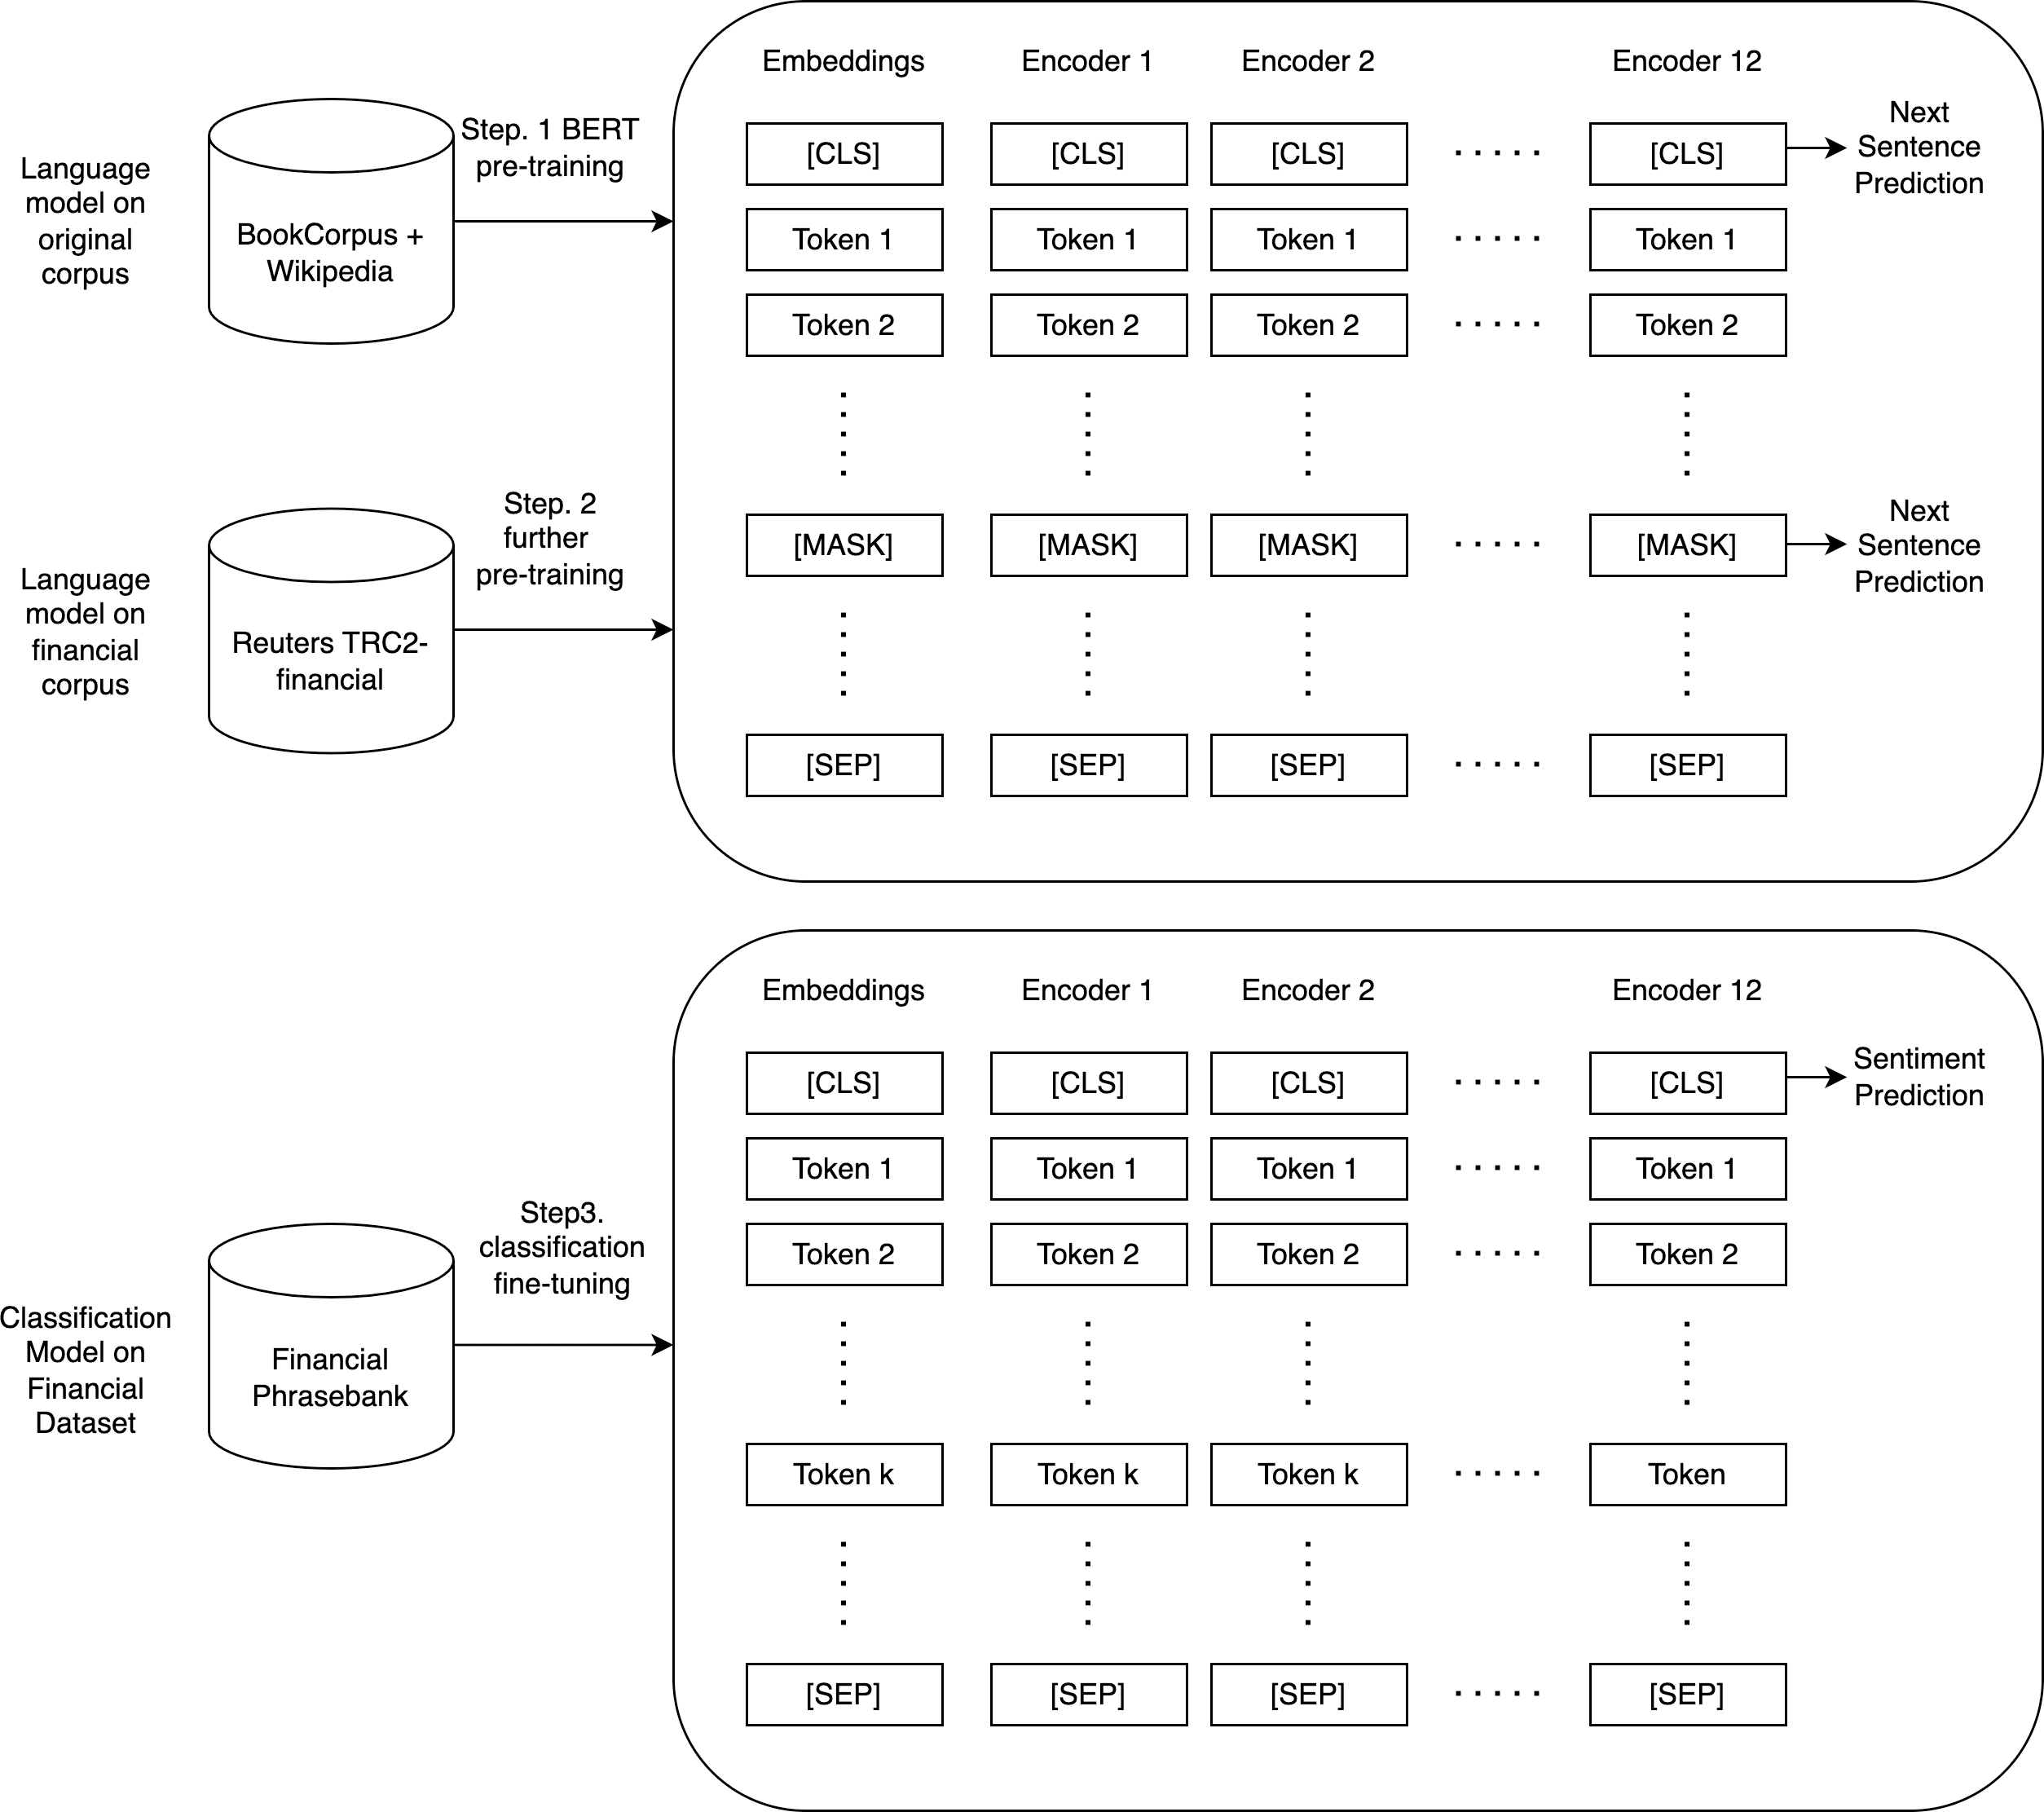
\includegraphics[width=0.85\linewidth]{gfx/m4l3_liu_fig2_pretraining_overview.png}
\par\smallskip{\small \textbf{Hình 2:} Tổng quan về huấn luyện trước, huấn luyện trước bổ sung, phân loại, và tinh chỉnh của FinBERT.}
\end{figure}

Fazlija \& Harder (2022) đã sử dụng mô hình FinBERT để phân loại tin tức, dự báo xu hướng giá cổ phiếu bằng bộ phân loại rừng ngẫu nhiên (random forest), và đo lường hiệu suất đầu tư của các mô hình. Hiệu suất của phương pháp được đề xuất trong nghiên cứu vượt trội hơn chỉ số S\&P 500. Tuy nhiên, mặc dù bài báo này sử dụng kiểm định chéo K-lần (K-fold cross-validation) để tìm tham số mô hình tốt nhất, chia tập dữ liệu huấn luyện và kiểm định thành nhiều bản sao, và huấn luyện nhiều mô hình để kiểm định, các tác giả không đề cập đến việc sử dụng phương pháp cửa sổ trượt trong nghiên cứu của họ. Do đó, trong nghiên cứu của chúng tôi, chúng tôi dự định áp dụng FinBERT để phân tích các bình luận trên mạng xã hội, cho phép chúng tôi thu thập nhiều ý kiến hơn về tài sản mục tiêu. Sau đó, bằng cách dự đoán sử dụng phương pháp cửa sổ trượt, chúng tôi không chỉ có thể tránh vấn đề thiên lệch nhìn trước, mà còn cập nhật dữ liệu huấn luyện theo thời gian, điều này có thể dẫn đến các dự đoán chính xác hơn.

Trong nghiên cứu này, chúng tôi đề xuất sử dụng FinBERT để thực hiện phân tích cảm xúc trên bình luận của nhà đầu tư trên Stocktwits nhằm dự đoán biến động giá cổ phiếu. Ít nghiên cứu đã sử dụng FinBERT để phân tích cảm xúc trên mạng xã hội. Tuy nhiên, chúng tôi tin rằng việc áp dụng nó cụ thể để phân tích bình luận Stocktwits, thay vì sử dụng mô hình phân tích cảm xúc hai lớp, sẽ cải thiện chỉ số cảm xúc ở mức vĩ mô và nâng cao độ chính xác của dự đoán biến động giá cổ phiếu.

\section{Phương pháp luận}

Trong mục này, chúng tôi thảo luận về các nguồn dữ liệu khác nhau có thể được sử dụng để phân tích cổ phiếu, chẳng hạn như dữ liệu lịch sử, bình luận, và dữ liệu cảm xúc. Chúng tôi cũng trình bày các bước tiền xử lý cần thiết để phân tích bình luận, bao gồm cách tính toán chỉ số cảm xúc. Cuối cùng, chúng tôi giới thiệu một mô hình dự đoán biến động giá cổ phiếu sử dụng các kỹ thuật tập hợp (ensemble) và máy vector hỗ trợ.

\subsection*{Thu thập dữ liệu}

Trên Stocktwits, người dùng có thể chia sẻ một tin nhắn và gán nhãn nó là ``tăng giá'' (bullish) hoặc ``giảm giá'' (bearish), hoặc họ có thể bỏ qua các cảm xúc này. Có ba cột dữ liệu: tin nhắn, ngày/giờ, và cảm xúc (tùy chọn). Các tin nhắn (tweets) trên Stocktwits được thể hiện trong Hình 3.

\begin{figure}[H]
\centering
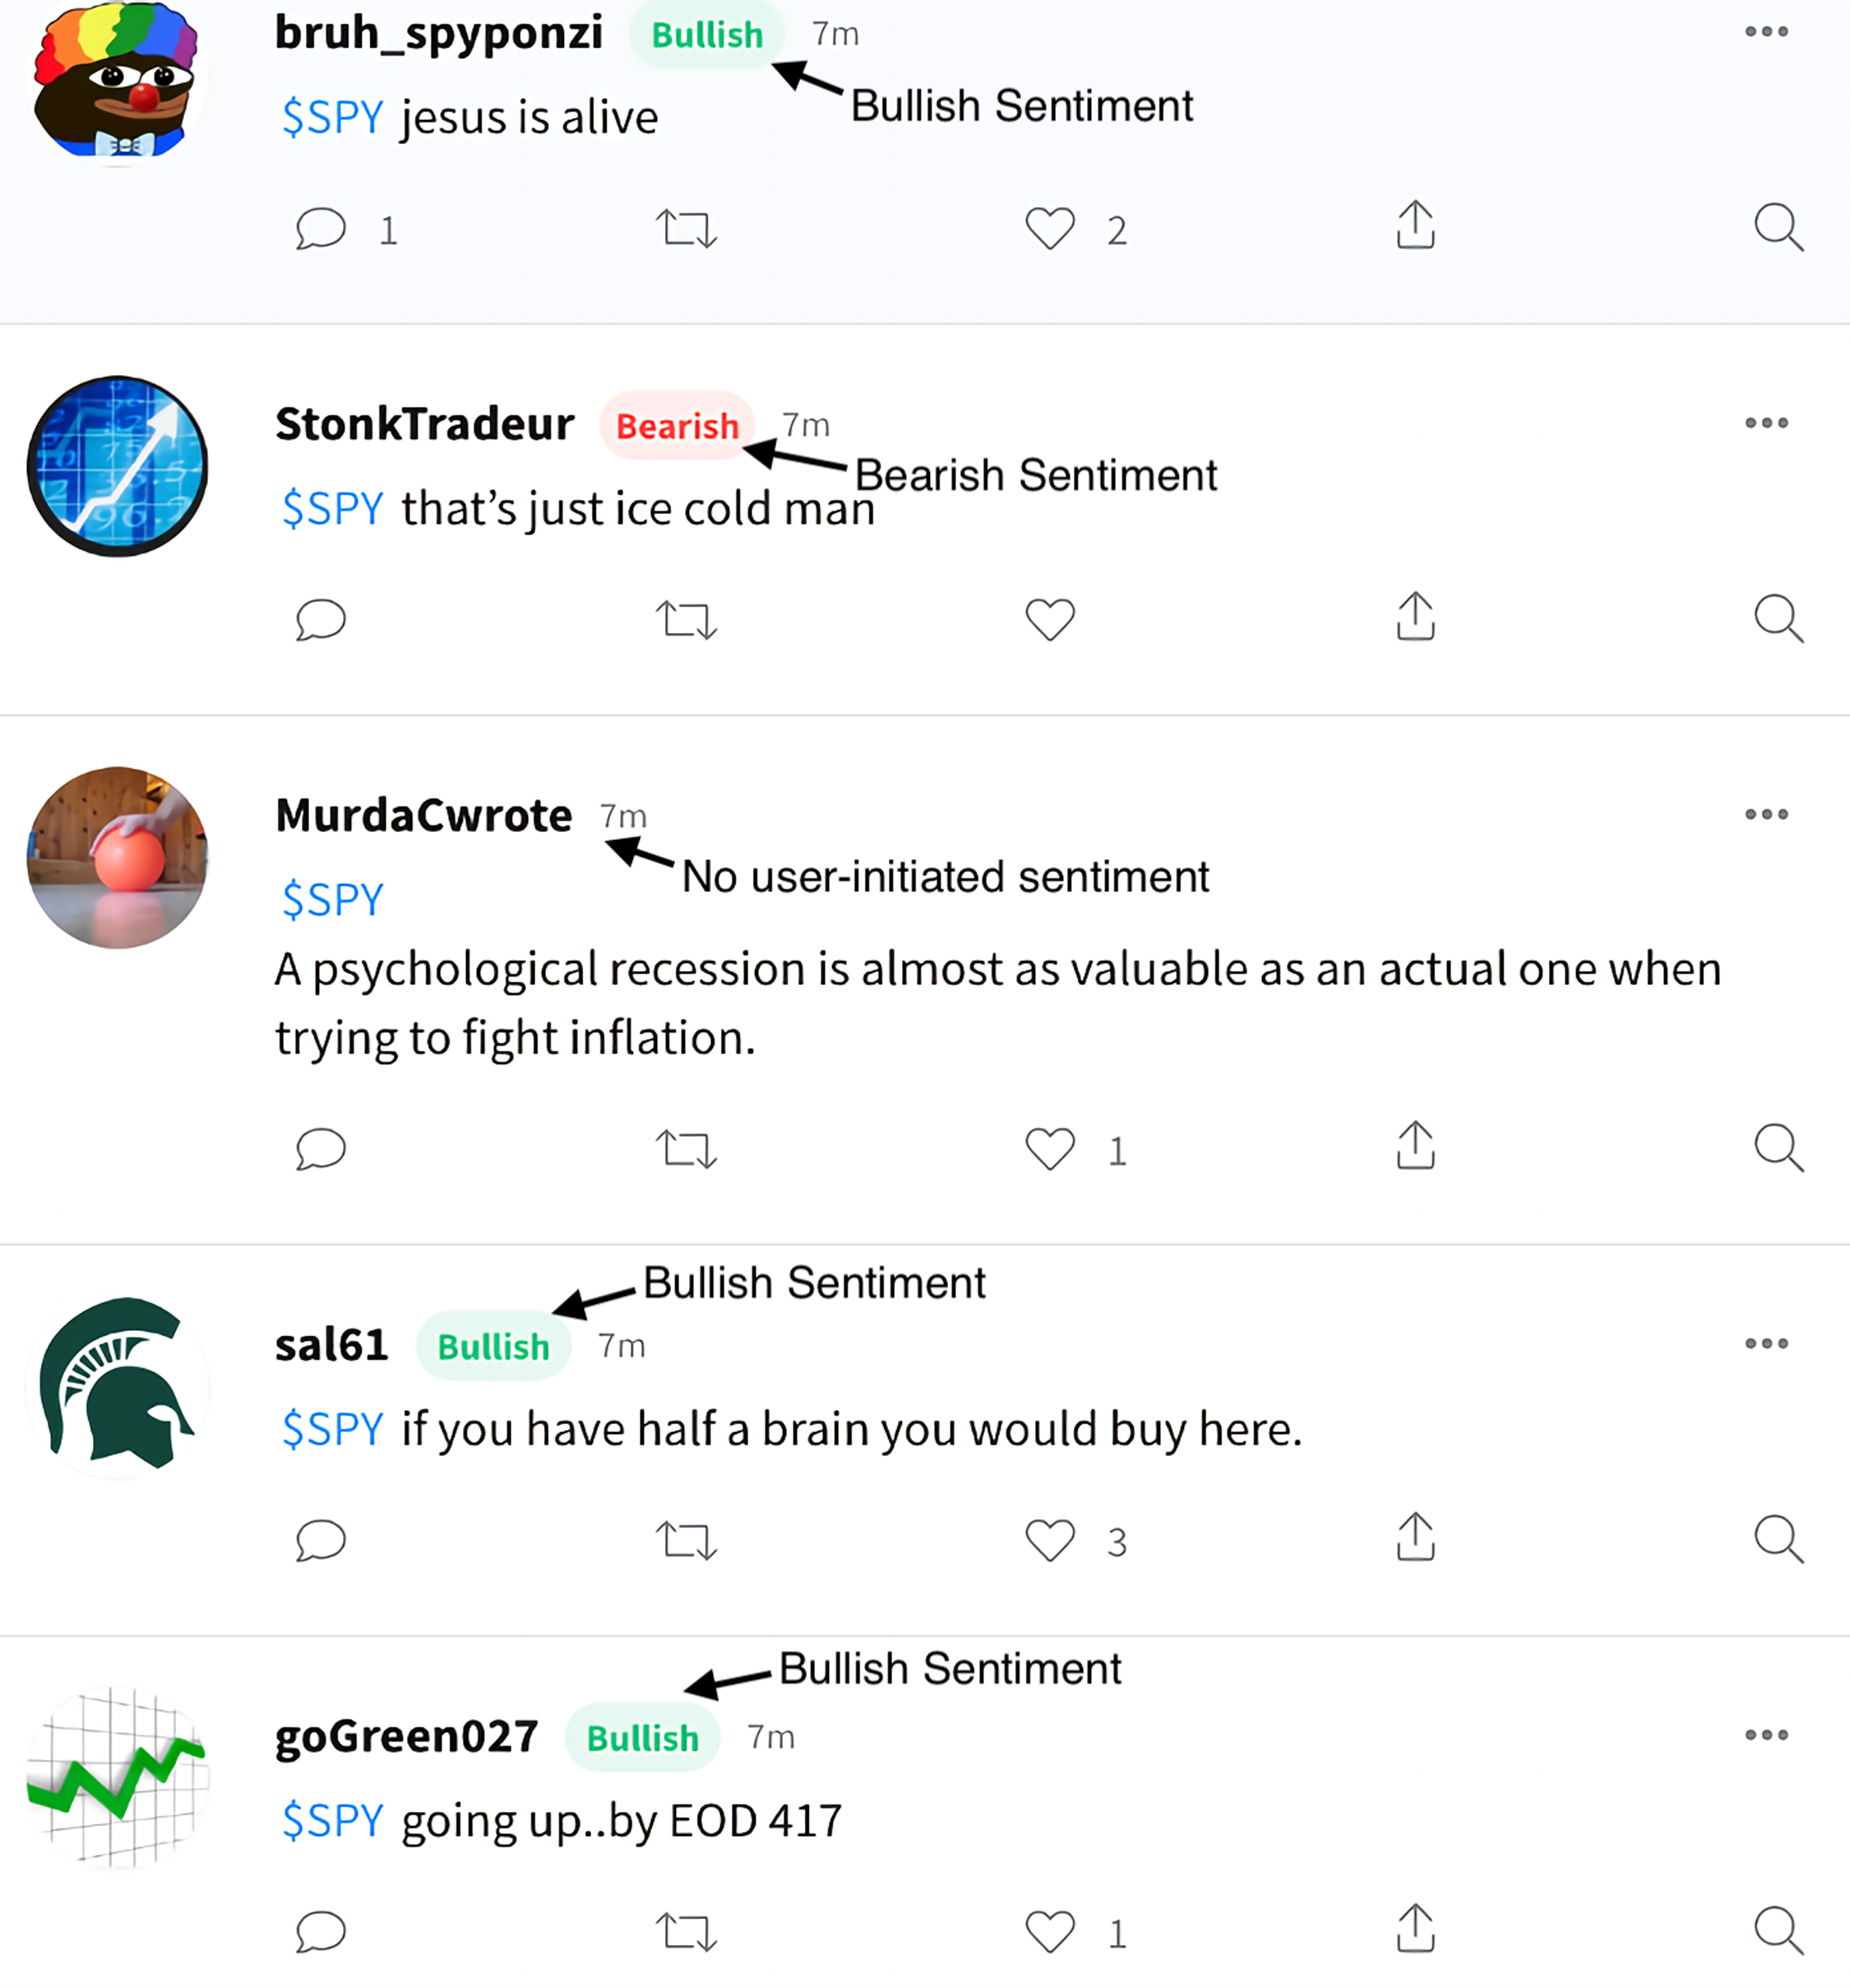
\includegraphics[width=0.6\linewidth]{gfx/m4l3_liu_fig3_tweets_stocktwits.png}
\par\smallskip{\small \textbf{Hình 3:} Các tin nhắn được người dùng đăng trên Stocktwits. Người dùng có thể điền văn bản và gán nhãn cảm xúc theo quan điểm của họ về tương lai (tùy chọn). Như có thể thấy trong hình, một số tin nhắn có cảm xúc tăng giá hoặc giảm giá, trong khi những tin nhắn khác không được gán nhãn.}
\end{figure}

Việc truy cập \url{https://api.Stocktwits.com/} cho phép chúng tôi xem xét các bình luận của nhà đầu tư ở định dạng JSON về một cổ phiếu nhất định từ Stocktwits. Để lấy dữ liệu từ Stocktwits, chúng tôi đã phát triển một ứng dụng Node.js tự động tải xuống và lưu các tệp CSV chứa tất cả bình luận về một cổ phiếu cụ thể trong một khoảng thời gian nhất định. Sau đó, chúng tôi đưa dữ liệu vào môi trường Python để thực hiện phân tích sâu hơn.

Dữ liệu cổ phiếu lịch sử được thu thập từ cnYES (\url{https://www.cnyes.com/}), và các cột dữ liệu bao gồm giá mở cửa, giá đóng cửa, giá cao nhất, giá thấp nhất của cổ phiếu, VWAP (giá bình quân gia quyền theo khối lượng), khối lượng, giá trị giao dịch, mức thay đổi, và phần trăm thay đổi, như được thể hiện trong Bảng 1.

\begin{figure}[H]
\centering
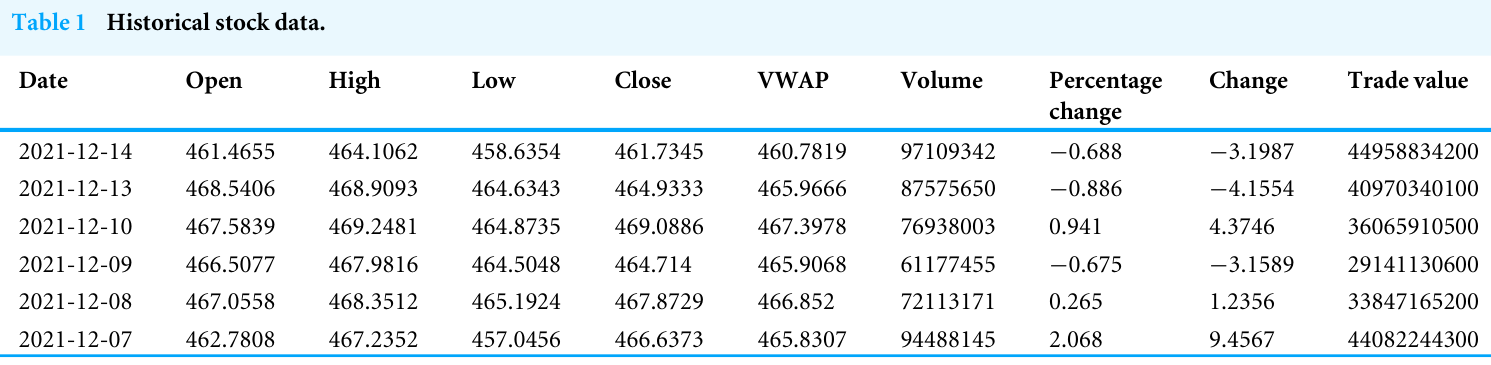
\includegraphics[width=0.95\linewidth]{gfx/m4l3_liu_table1_historical_stock_data.png}
\par\smallskip{\small \textbf{Bảng 1:} Dữ liệu cổ phiếu lịch sử.}
\end{figure}

Chúng tôi đã sử dụng AlphaVantage API (\url{https://www.alphavantage.co/}) để lấy dữ liệu giá cổ phiếu lịch sử theo thời gian thực. Điều này cho phép chúng tôi nắm được thông tin chi tiết về giá cổ phiếu theo từng phút, giúp chúng tôi đưa ra các dự báo linh hoạt hơn. Tuy nhiên, dữ liệu bị giới hạn trong hai năm gần nhất. Bảng 2 cho thấy dữ liệu giá cổ phiếu lịch sử với bước thời gian 15 phút.

\begin{figure}[H]
\centering
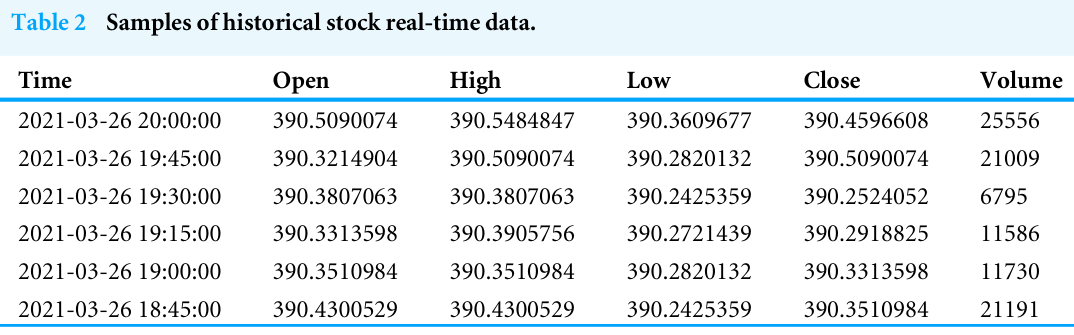
\includegraphics[width=0.85\linewidth]{gfx/m4l3_liu_table2_realtime_data_samples.png}
\par\smallskip{\small \textbf{Bảng 2:} Mẫu dữ liệu giá cổ phiếu lịch sử thời gian thực.}
\end{figure}

\subsection*{Tiền xử lý dữ liệu cảm xúc}

Chúng tôi tham khảo Cao và cộng sự (2022). Trước khi thực hiện phân tích cảm xúc, các bước tiền xử lý văn bản sau đây cần được thực hiện:
\begin{enumerate}
  \item Loại bỏ tất cả các liên kết web khỏi văn bản, bao gồm cả những liên kết bắt đầu bằng ``http://'', ``https://'', hoặc ``www.''.
  \item Thay thế ký tự HTML cho dấu nháy đơn bằng dấu nháy đơn tiêu chuẩn.
  \item Nhận diện và thay thế các hashtag (\#) và cashtag (\$) trong văn bản. Tìm tất cả các từ bắt đầu bằng ``\#'' hoặc ``\$'', chẳng hạn như \$AAPL, và thay thế chúng bằng các thuật ngữ như ``cashtag\_AAPL''. Sự thay đổi này được thực hiện nhằm bảo toàn thông tin ký hiệu gốc đồng thời làm cho nó phù hợp hơn cho việc xử lý văn bản.
  \item Thay thế tên người dùng Twitter bằng một thuật ngữ bắt đầu bằng ``mention\_'', theo sau là tên người dùng. Sửa đổi này cũng nhằm mục đích bảo toàn thông tin gốc trong khi làm cho nó phù hợp hơn cho việc xử lý văn bản.
  \item Chuyển đổi tất cả biểu tượng cảm xúc (emoji) thành mô tả văn bản tương ứng để duy trì thông tin cảm xúc hoặc ngữ nghĩa mà chúng truyền tải, nhưng ở một định dạng dễ hiểu hơn đối với mô hình.
\end{enumerate}

\subsection*{Dự đoán biến động giá cổ phiếu}

Kiến trúc được mô tả trong Hình 4 được sử dụng để dự đoán biến động giá cổ phiếu. Chúng tôi thu thập dữ liệu cần thiết, được chia thành hai phần: phần đầu tiên bao gồm các bình luận về các cổ phiếu cụ thể trên Stocktwits, một số trong đó không được gán nhãn tăng giá hoặc giảm giá, trong khi phần thứ hai bao gồm dữ liệu lịch sử về giá cổ phiếu. Chúng tôi có thể chọn sử dụng mô hình phân tích cảm xúc hai lớp để gán nhãn các bình luận chưa được gán nhãn hoặc sử dụng mô hình phân tích cảm xúc ba lớp như FinBERT hoặc VADER để gán nhãn tất cả bình luận. Cuối cùng, chúng tôi áp dụng công thức chỉ số cảm xúc để tính chỉ số thực thể (entity index) của các bình luận từ nhiều giai đoạn khác nhau. Để dự đoán biến động giá cổ phiếu, chúng tôi kết hợp các chỉ số cảm xúc với dữ liệu cổ phiếu lịch sử làm đặc trưng và đưa chúng vào một mô hình dự đoán được thiết kế cho biến động giá cổ phiếu. Chúng tôi đã sử dụng phương pháp cửa sổ trượt để dự đoán và phân tích độ chính xác của các dự đoán biến động cổ phiếu.

\begin{figure}[H]
\centering
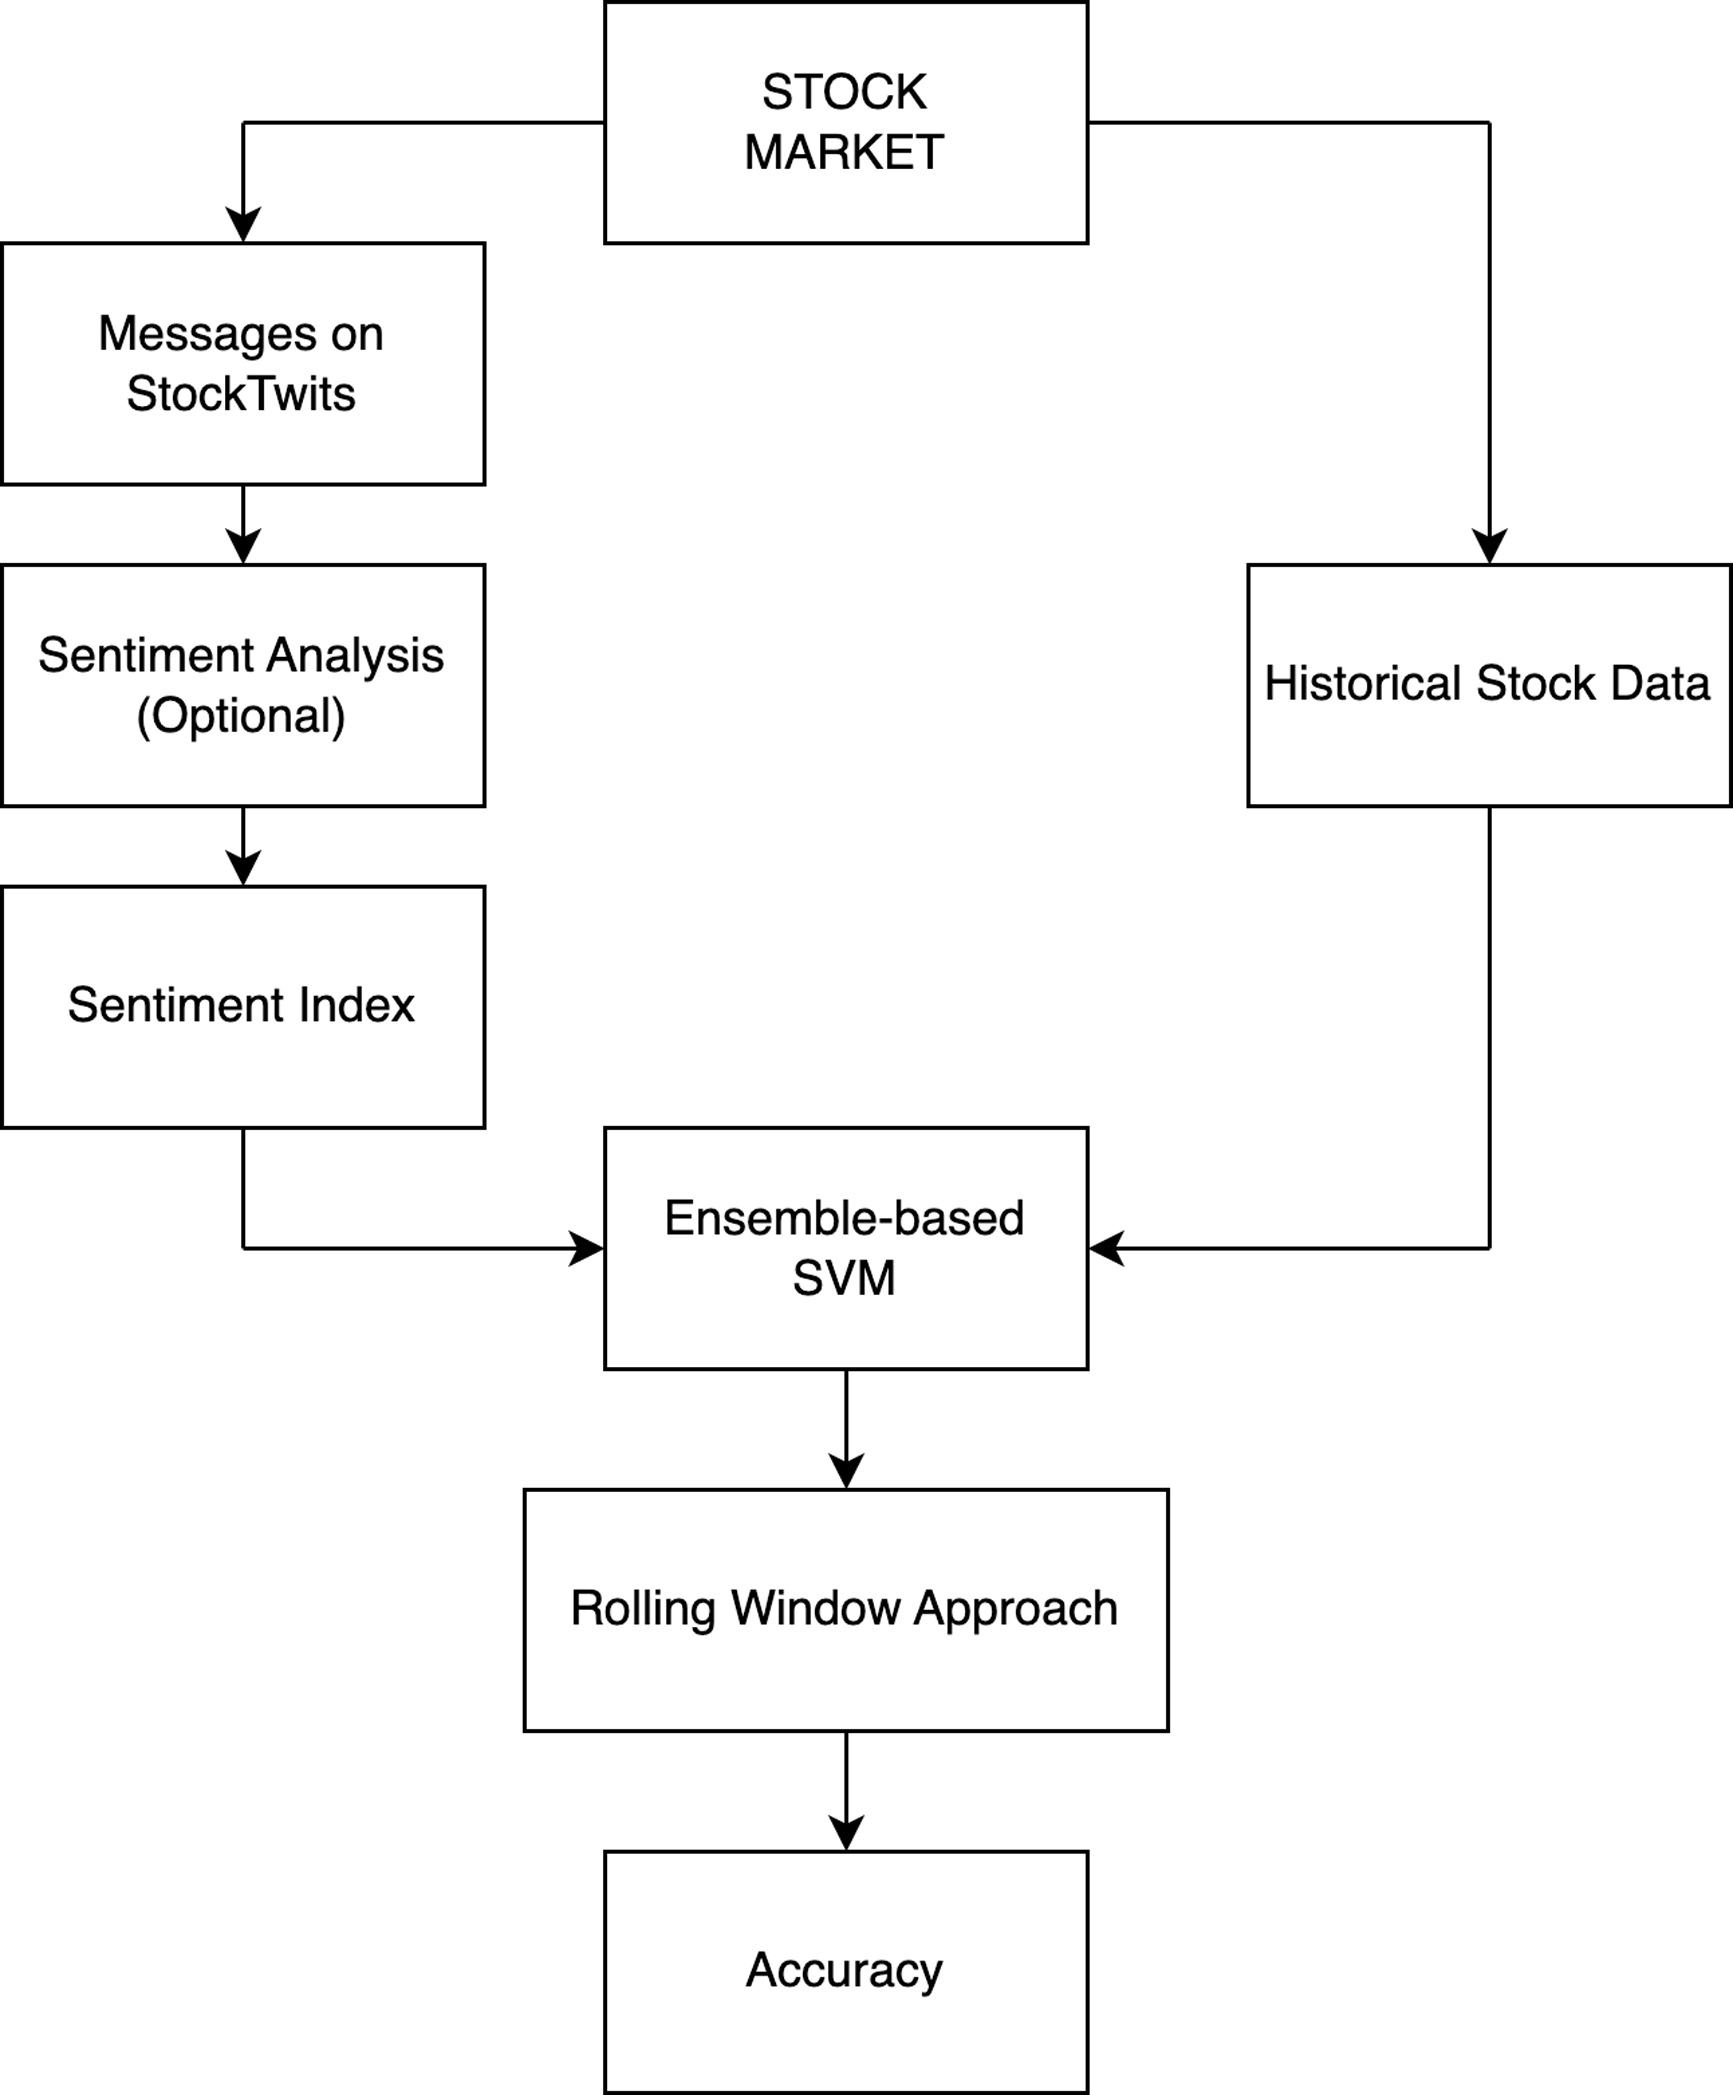
\includegraphics[width=0.55\linewidth]{gfx/m4l3_liu_fig4_prediction_architecture.png}
\par\smallskip{\small \textbf{Hình 4:} Tổng quan kiến trúc dự đoán biến động thị trường chứng khoán.}
\end{figure}

\subsection*{Tính toán chỉ số cảm xúc}

Cách tính chỉ số cảm xúc hai lớp được sử dụng trong bài báo này tham khảo phương pháp của Antweiler \& Frank (2004).

$$
S_t = \ln\left[\frac{1+M_t^{pos}}{1+M_t^{neg}}\right]
$$

Chỉ số này cho phép chúng ta tính toán cảm xúc cho một giai đoạn, trong đó $M_t^{pos}$, $M_t^{neg}$ là số lượng tin nhắn tích cực và tiêu cực trong giai đoạn đó. Nếu chỉ số cảm xúc dương, cảm xúc thị trường là lạc quan. Nếu chỉ số cảm xúc âm, cảm xúc thị trường là bi quan. Nếu chỉ số cảm xúc bằng không, cảm xúc thị trường là trung lập. Chỉ số này giúp chúng tôi xác định cảm xúc nhà đầu tư trong một khoảng thời gian nhất định và cũng điều chỉnh cho các tín hiệu quá lạc quan hoặc quá bi quan trong quá trình tính toán.

Đối với các mô hình phân tích cảm xúc ba lớp (bao gồm cảm xúc tích cực, tiêu cực, và trung lập), tham khảo phương trình được sử dụng để tính chỉ số cảm xúc trong Hiew và cộng sự (2019).

$$
S_t = \frac{M_t^{pos} - M_t^{neg}}{M_t^{pos} + M_t^{neu} + M_t^{neg}}
$$

trong đó $M_t^{pos}$, $M_t^{neg}$, $M_t^{neu}$ là số lượng tin nhắn tích cực, tiêu cực và trung lập trong giai đoạn đó.

\subsection*{Máy vector hỗ trợ}

Máy vector hỗ trợ (SVM) là một thuật toán học máy có giám sát được phát triển bởi Cortes \& Vapnik (1995), có thể được sử dụng để giải quyết các bài toán phân loại và hồi quy. Khái niệm này khá đơn giản: tìm một ranh giới quyết định (decision boundary) tối đa hóa biên (margin) giữa hai lớp, như được thể hiện trong Hình 5.

\begin{figure}[H]
\centering
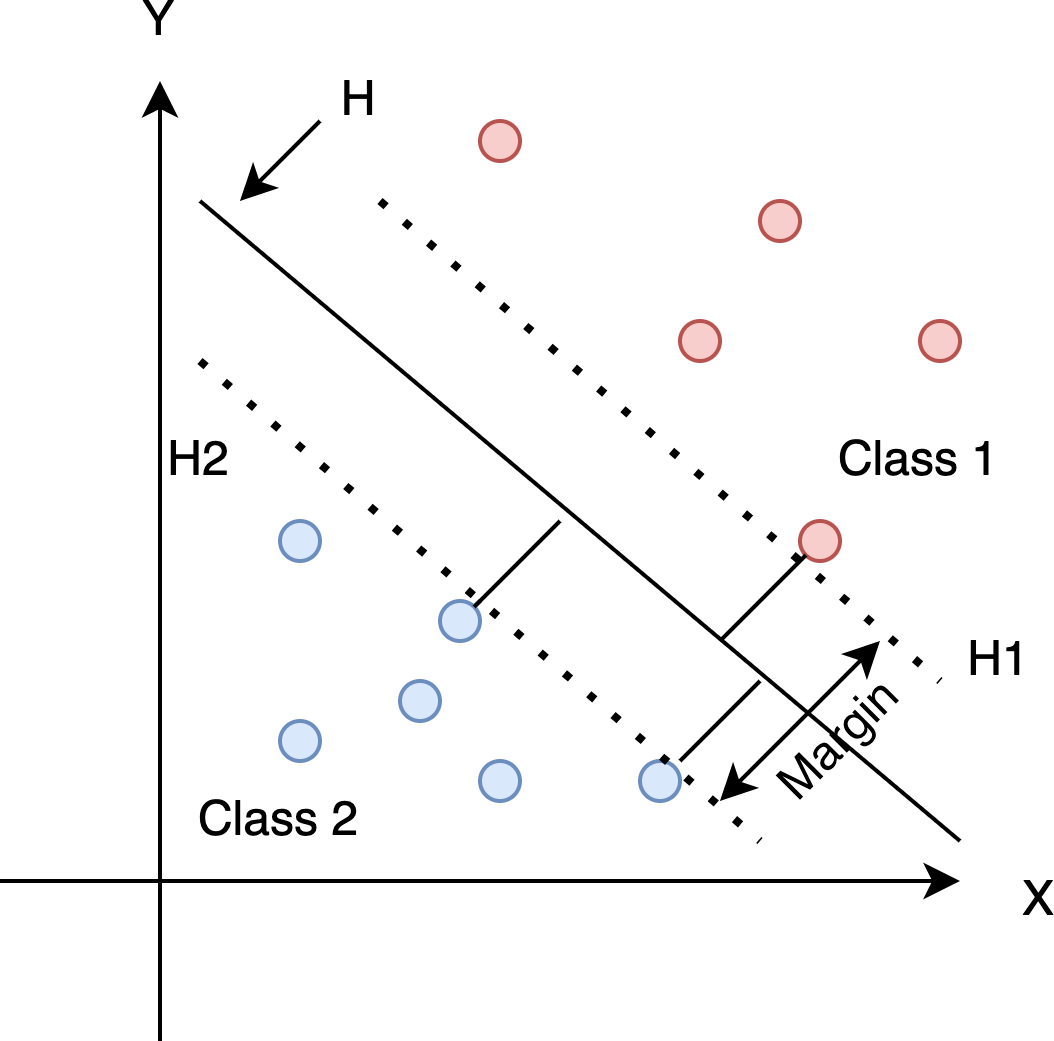
\includegraphics[width=0.6\linewidth]{gfx/m4l3_liu_fig5_svm_hyperplane.png}
\par\smallskip{\small \textbf{Hình 5:} Tìm siêu phẳng (hyperplane) tối ưu phân tách tập dữ liệu thành hai loại.}
\end{figure}

Khoảng cách từ điểm $(x, y)$ đến đường thẳng $Ax+By+C=0$ được cho bởi

$$
\frac{Ax+By+C}{\sqrt{A^2+B^2}}
$$

Mở rộng nó sang không gian $n$ chiều, chúng ta biểu diễn nó là $w^T x + b = 0$, và khoảng cách là

$$
\frac{(w^T x + b)}{\lVert w \rVert}
$$

trong đó $w$ biểu thị trọng số của mỗi đặc trưng, $b$ biểu thị hệ số chặn (intercept).

Nếu chúng ta bỏ qua vấn đề dữ liệu trộn lẫn, tức là nếu tất cả dữ liệu có thể được phân loại hoàn hảo, chúng ta gọi đây là SVM biên cứng (hard-margin SVM) và phân chia hai lớp theo phương trình dưới đây.

$$
\begin{cases}
w^T x^{(i)} + b \geq 1, & \forall y^{(i)} = 1 \\
w^T x^{(i)} + b \leq -1, & \forall y^{(i)} = -1
\end{cases}
$$

Và đơn giản hóa công thức như sau

$$
y^{(i)}\left(w^T x^{(i)} + b\right) \geq 1, \quad \forall i = 1, \dots, n
$$

Nghiệm của SVM là một bài toán tối ưu hóa đơn giản. Trong một số điều kiện, khoảng cách biên giữa hai lớp càng lớn thì càng tốt. Công thức như sau

$$
\min \frac{1}{2} \lVert w \rVert^2
$$

$$
\text{s.t.} \quad y_i\left(w^T x_i + b\right) \geq 0, \quad \forall i = 1, \dots, n
$$

Tuy nhiên, hiếm khi dữ liệu thực tế bao gồm các ví dụ có thể được xác định chính xác. Do đó, chúng ta cho phép một số điểm nhất định vượt qua ranh giới quyết định ban đầu và cho phép một số mẫu bất thường bị phân loại sai. Mặc dù điều này có thể dẫn đến việc phân loại sai, khả năng tổng quát hóa có thể tốt hơn trong các ứng dụng thực tế. Loại SVM này được gọi là SVM biên mềm (soft-margin SVM), sử dụng công thức sau

$$
\min_{w, \xi_i} \frac{1}{2} w^T w + C \sum_{i=1}^{n} \xi_i
$$

$$
\text{s.t.} \quad y_i\left(w^T x_i + b\right) \geq 1 - \xi_i, \; \xi_i \geq 0, \; \forall i = 1, \dots, n
$$

trong đó $\xi_i$ là một sai số huấn luyện có thể chấp nhận được, và $C$ xác định mức trọng số phạt cần được đưa ra.

Từ phương trình trên, chúng ta có thể thấy rằng nếu $C$ lớn hơn, mức dung sai đối với lỗi nhỏ hơn, và nếu $C$ tiến tới dương vô cực, nó sẽ trở thành SVM biên cứng. Ngược lại, nếu $C$ nhỏ hơn, mức dung sai đối với lỗi lớn hơn.

Để giải nghiệm tối ưu của bài toán gốc (primal problem), chúng ta có thể chuyển đổi nó thành bài toán đối ngẫu (dual problem), như được thể hiện trong phương trình sau

$$
\max_{\alpha} \sum_{i=1}^{n} \alpha_i - \frac{1}{2} \sum_{i=1}^{n} \sum_{j=1}^{n} \alpha_i \alpha_j y_i y_j K(x_i, x_j)
$$

$$
\text{s.t.} \quad \sum_{i=1}^{n} \alpha_i y_i = 0
$$

$$
0 \leq \alpha_i \leq C, \quad \forall i = 1, \dots, n
$$

trong đó $\boldsymbol{\alpha} = (\alpha_1, \dots, \alpha_n)^T$ là nhân tử Lagrange, và $K(x_i, x_j)$ biểu thị việc chúng ta sử dụng một hàm nhân (kernel) để định nghĩa lại tích trong (inner product) của $x_i$ và $x_j$. Có một số hàm nhân phổ biến được thể hiện trong Bảng 3.

\begin{figure}[H]
\centering
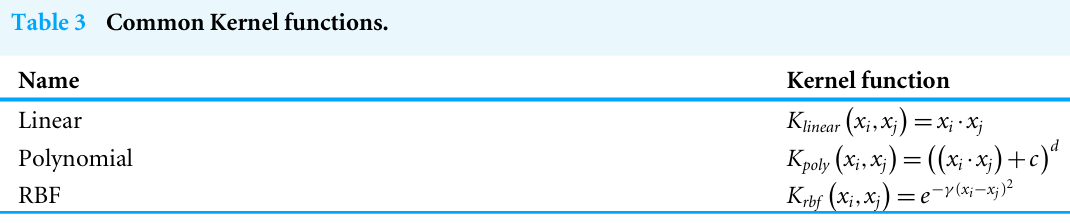
\includegraphics[width=0.9\linewidth]{gfx/m4l3_liu_table3_kernel_functions.png}
\par\smallskip{\small \textbf{Bảng 3:} Các hàm nhân (kernel function) phổ biến.}
\end{figure}

Cuối cùng, hàm quyết định $D(x) = \operatorname{sgn}(w^* \cdot x + b^*)$ được cho bởi

$$
D(x) = \operatorname{sgn}\left(\sum_{i=1}^{n} y_i \alpha_i * K(x_i, x_j) + b^*\right)
$$

$$
b^* = y_j - \sum_{i=1}^{n} y_i \alpha_i * K(x_i, x_j)
$$

\subsection*{Kỹ thuật dựa trên tập hợp (ensemble)}

Theo Mohareb và cộng sự (2016), kỹ thuật dựa trên tập hợp (ensemble-based) dựa trên việc phát triển nhiều bộ phân loại, với đầu ra dự đoán cuối cùng là sự tổng hợp của tất cả các kết quả phân loại trong tập hợp đó. Giả sử chúng ta sử dụng $n$ bộ phân loại $\varepsilon = \{C_1, \dots, C_n\}$ để dự đoán một mẫu, nếu kết quả của $C_1$ sai, nhưng kết quả của $C_2, \dots, C_n$ đúng, thì kết quả có thể được phân loại chính xác bằng cách bỏ phiếu đa số (majority voting).

Các bộ phân loại riêng lẻ phải có độ chính xác tốt để phương pháp này khả thi. Nếu có tổng cộng $T$ bộ phân loại cho một bài toán $c$ lớp, lựa chọn tập hợp sẽ đúng nếu ít nhất $[T/c+1]$ bộ phân loại chọn đúng lớp. Giả sử mỗi bộ phân loại của $\varepsilon$ có xác suất $p$ chọn đúng lớp. Xác suất tập hợp chọn đúng lớp tuân theo phân phối nhị thức, và xác suất chọn được $k > T/c+1$ bộ phân loại đúng trong số $T$ được tính như sau (Mohareb và cộng sự, 2016):

$$
p_\varepsilon = \sum_{k=(T/c)+1}^{T} \binom{T}{k} p^k (1-p)^{(T-k)}
$$

\subsection*{Tập hợp SVM với bagging}

Theo Kim và cộng sự (2002), trong bagging, nhiều SVM được huấn luyện riêng lẻ bằng phương pháp bootstrap và sau đó được tổng hợp bằng một kỹ thuật kết hợp phù hợp. Tập huấn luyện cần được chia thành $L$ tập con để xây dựng tập hợp SVM với $L$ máy SVM độc lập. Dựa trên bằng chứng thống kê, cần làm cho các tập huấn luyện đa dạng nhất có thể để đạt được cải thiện lớn hơn trong kết quả tổng hợp. Chúng tôi áp dụng phương pháp bootstrap để thực hiện điều này.

Phương pháp bootstrap được đề xuất bởi Efron (1979). Nói một cách đơn giản, mỗi mô hình được huấn luyện bằng cách chọn ngẫu nhiên $n$ mẫu dữ liệu từ tập huấn luyện, và mỗi mẫu được trả lại tập huấn luyện sau khi chọn, như được thể hiện trong Hình 6.

\begin{figure}[H]
\centering
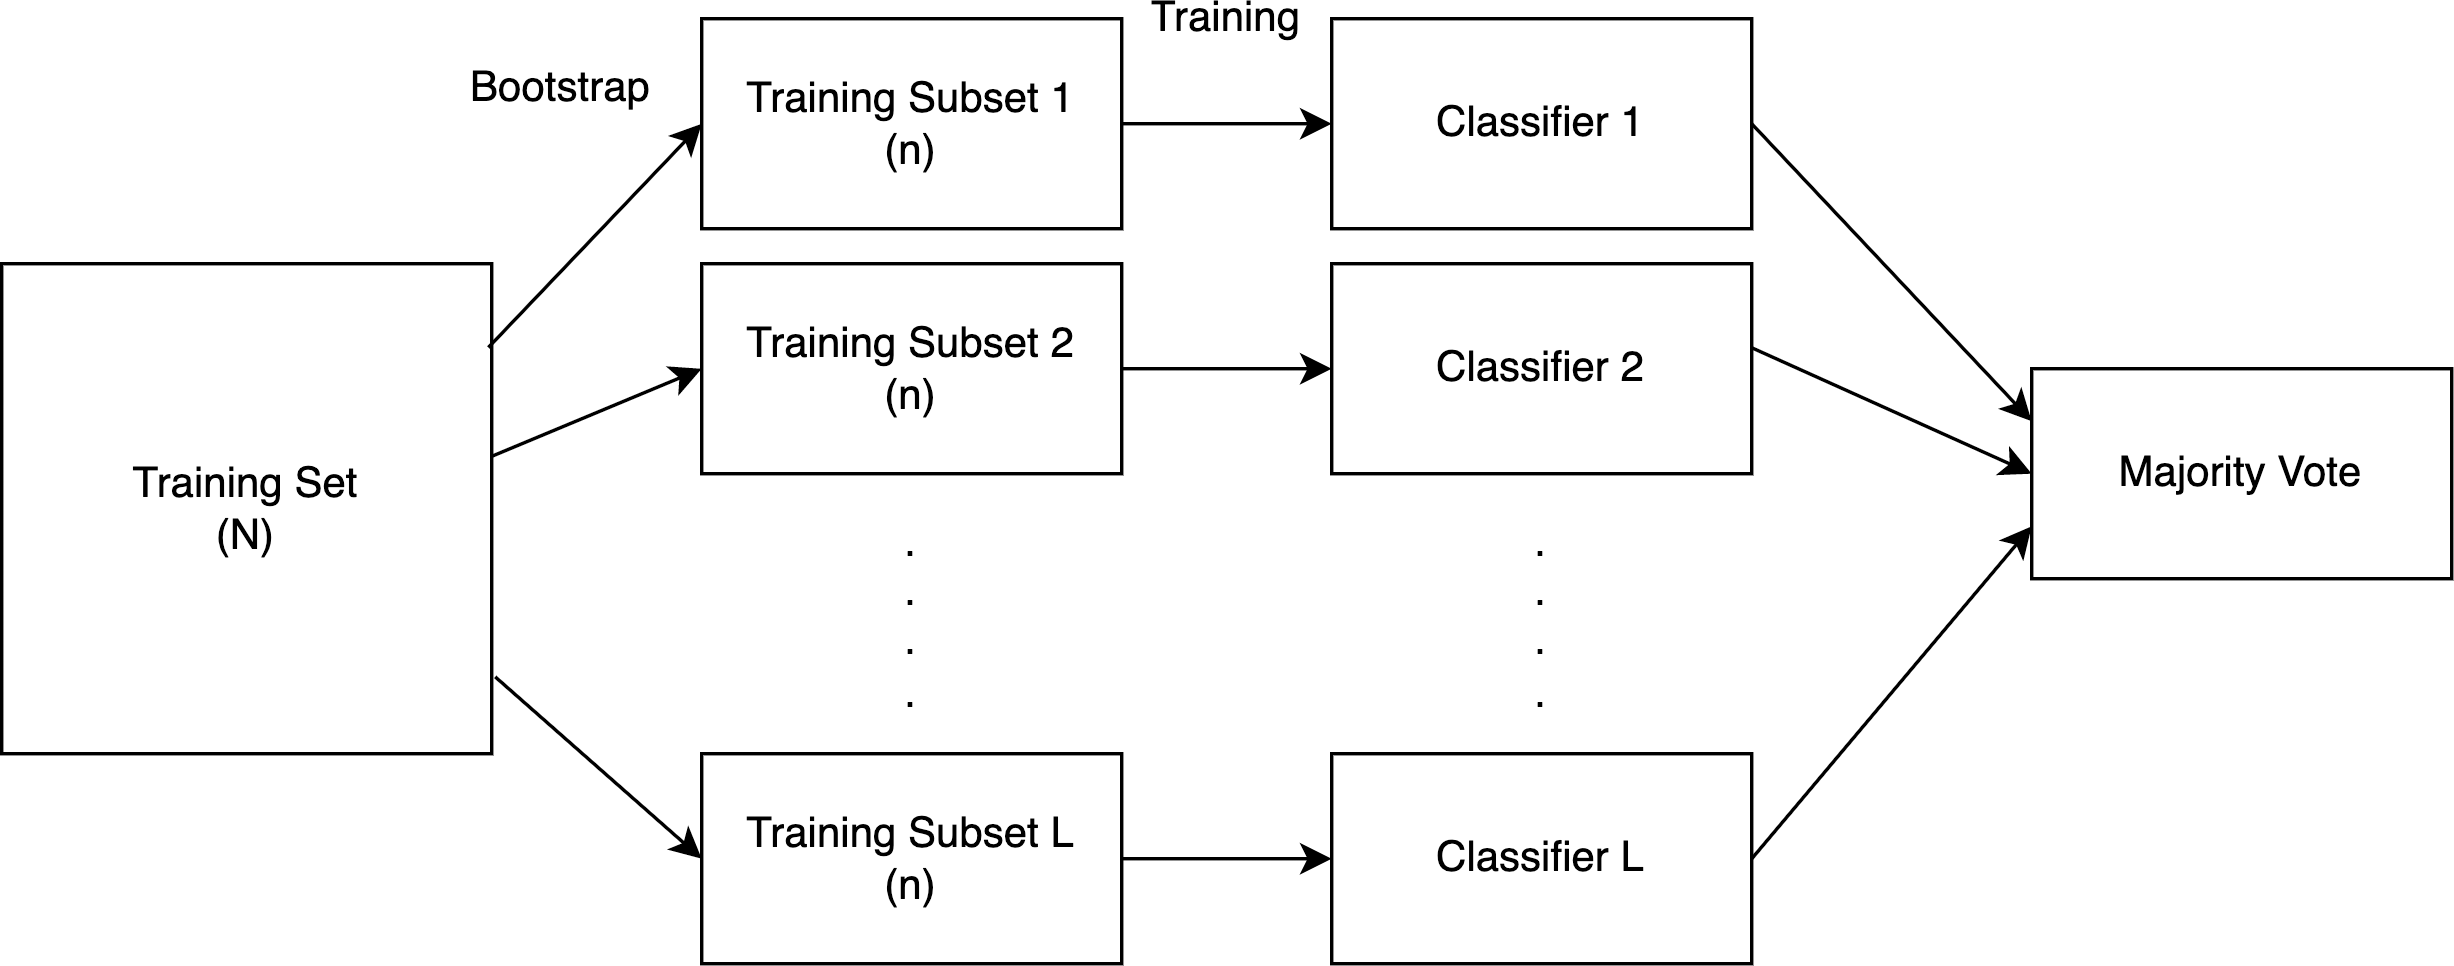
\includegraphics[width=0.85\linewidth]{gfx/m4l3_liu_fig6_bagging_procedure.png}
\par\smallskip{\small \textbf{Hình 6:} Sơ đồ biểu diễn quy trình bagging.}
\end{figure}

Chúng tôi sẽ sử dụng các mô hình với các tập con đã huấn luyện để dự báo dữ liệu kiểm định, và dự đoán cuối cùng sẽ được tạo ra từ các mô hình này thông qua bỏ phiếu đa số, như được giải thích dưới đây.

Bỏ phiếu đa số (majority vote) là phương pháp đơn giản nhất để kết hợp các bộ phân loại. Kết quả từ nhiều bộ phân loại được kết hợp bằng bỏ phiếu đa số. Đầu ra nhận được nhiều phiếu nhất sau đó được chọn làm quyết định phân loại cuối cùng (Kim \& Upneja, 2021).

\section{Thiết lập thực nghiệm}

Mục này trình bày thiết lập thực nghiệm, bao gồm chuẩn bị dữ liệu, trích xuất đặc trưng, xây dựng mô hình, và các chỉ số đánh giá.

\subsection*{Chuẩn bị dữ liệu}

Quỹ hoán đổi danh mục chỉ số SPDR S\&P 500 (SPY) đã được sử dụng trong nghiên cứu này vì đây hiện là quỹ hoán đổi danh mục (Exchange Traded Fund, ETF) S\&P 500 phổ biến nhất và là một trong những cổ phiếu có nhiều thảo luận nhất trên Stocktwits. Như được thể hiện trong Hình 7, đây là hạng mục hoạt động sôi nổi nhất trên Stocktwits vào ngày 7 tháng 9 năm 2022. Như có thể thấy, SPY có số lượng thảo luận nhiều hơn đáng kể so với bất kỳ cổ phiếu nào khác, và dựa trên quan sát của chúng tôi, SPY đã nằm trong top 3 trong một thời gian dài.

\begin{figure}[H]
\centering
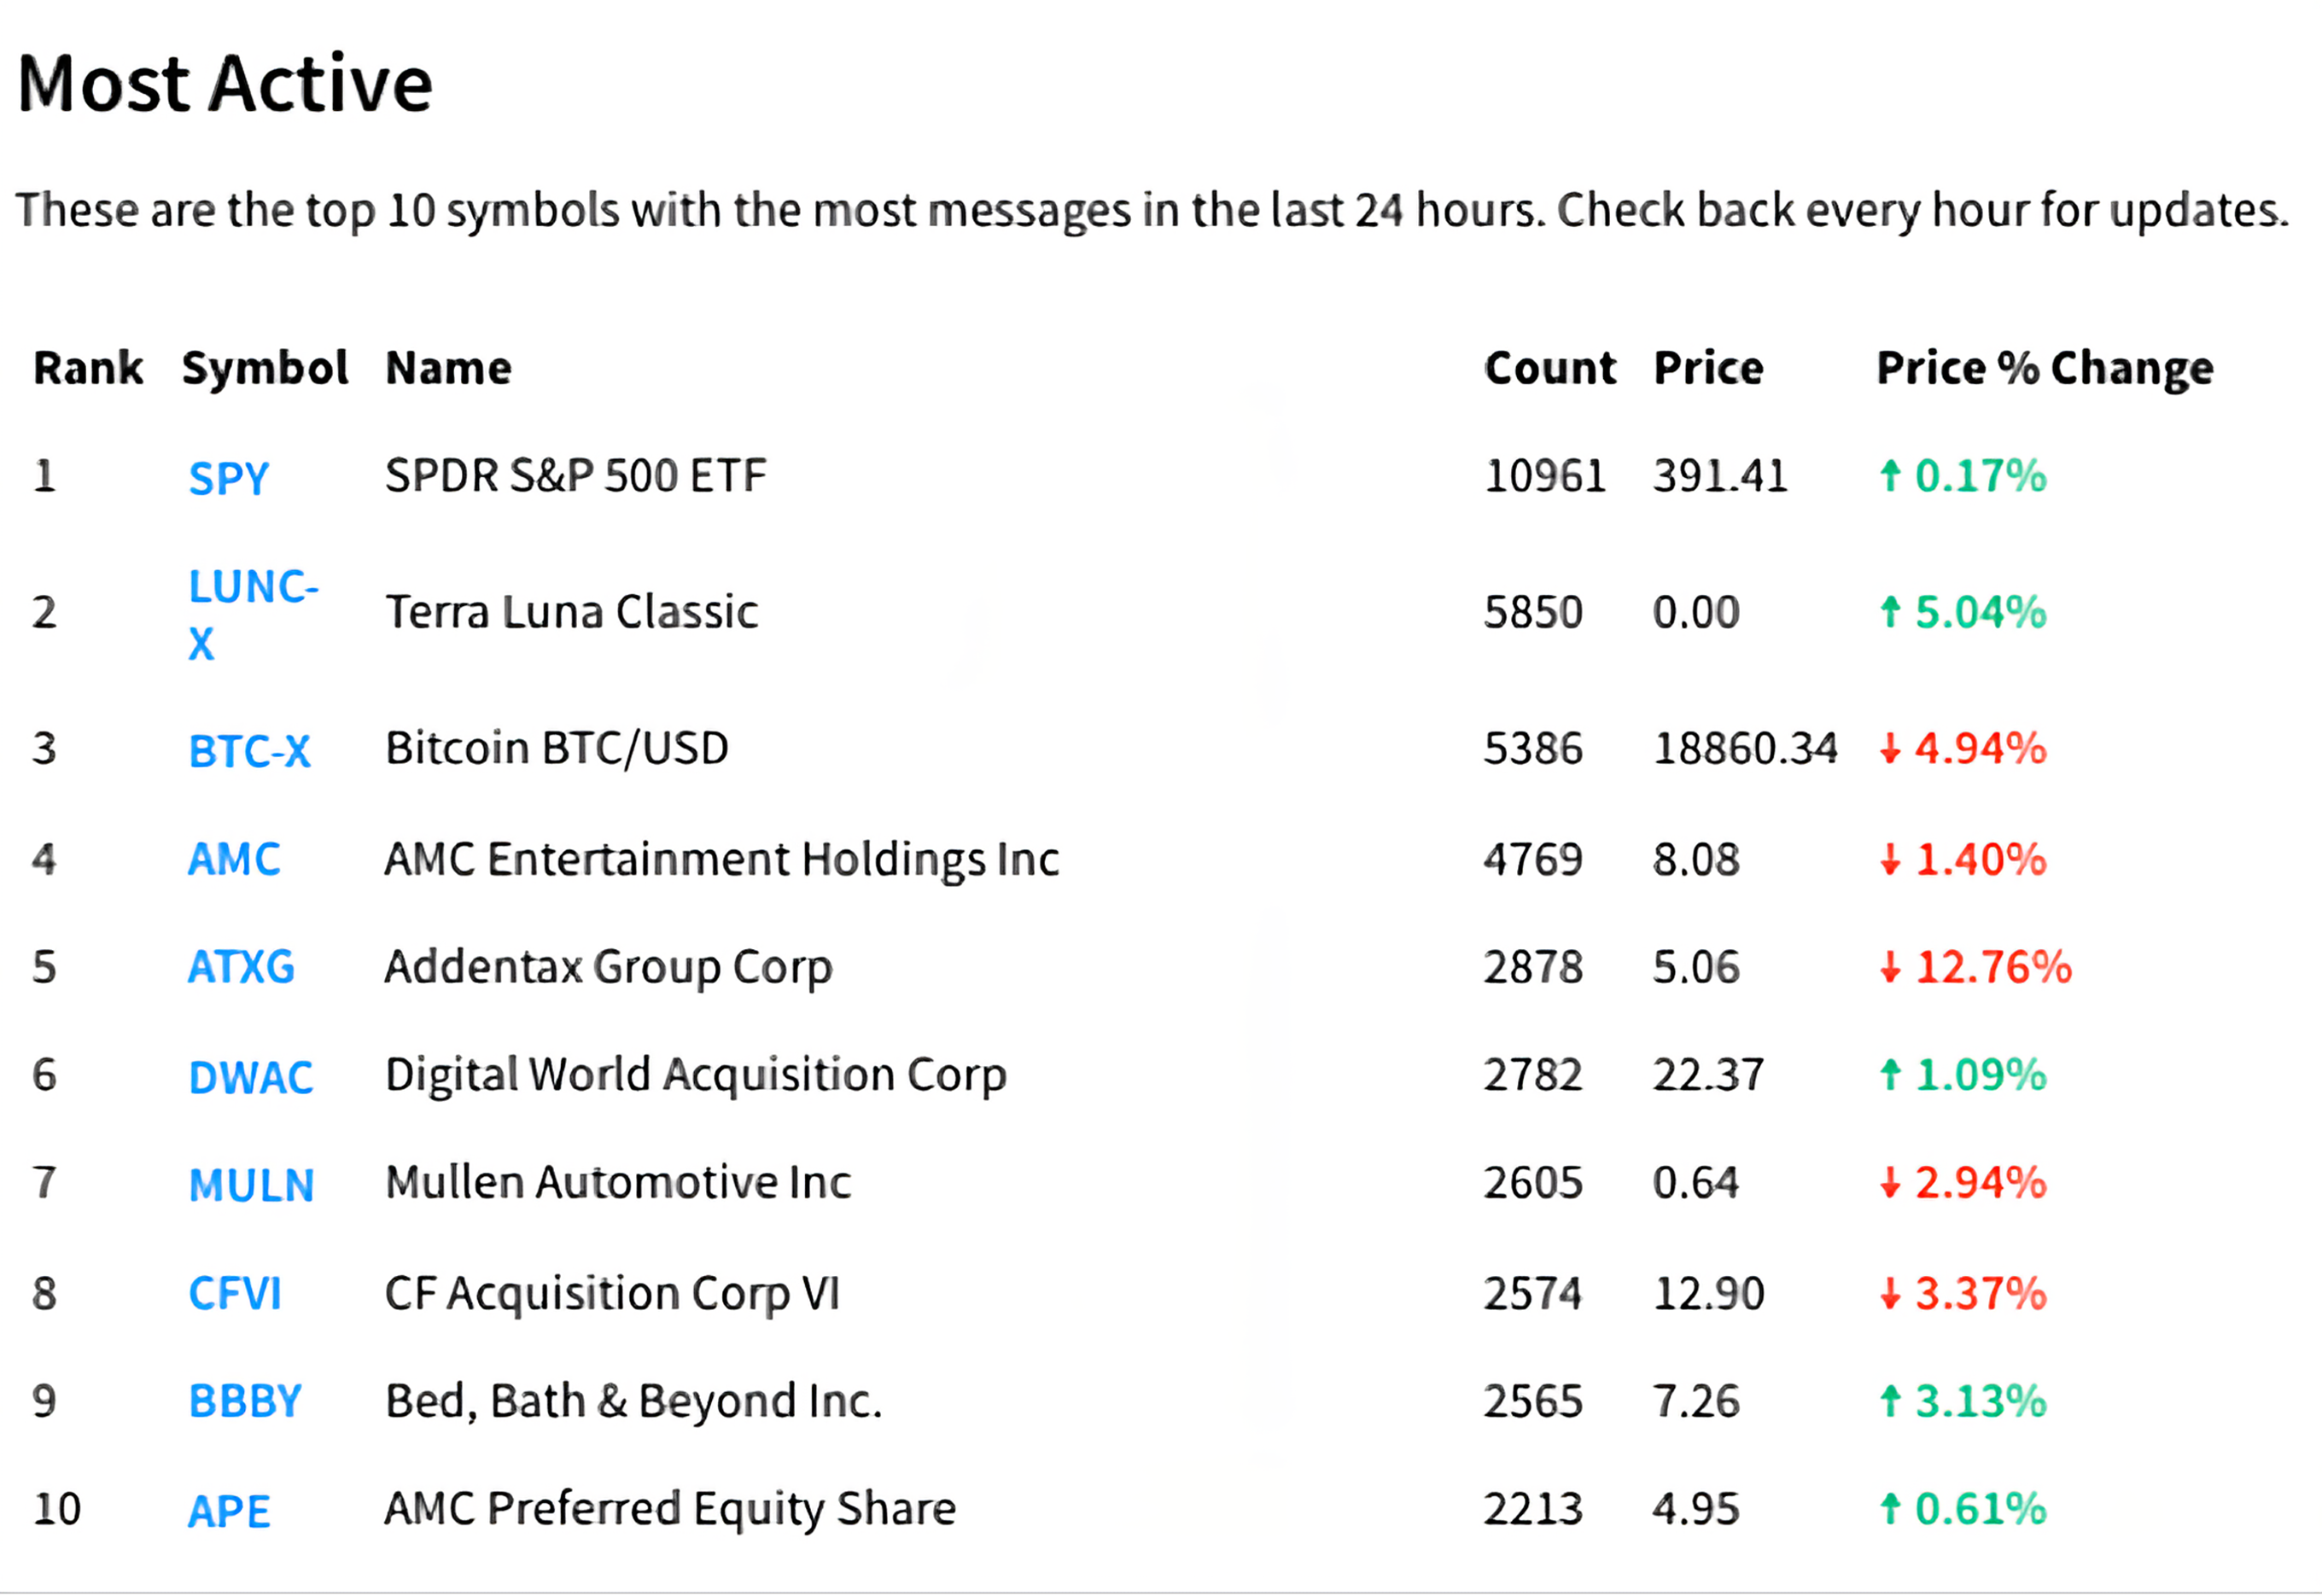
\includegraphics[width=0.85\linewidth]{gfx/m4l3_liu_fig7_top10_symbols.png}
\par\smallskip{\small \textbf{Hình 7:} Top 10 mã cổ phiếu có nhiều tin nhắn nhất vào ngày 7 tháng 9 năm 2022.}
\end{figure}

Chúng tôi thu thập tất cả bình luận về SPY và dữ liệu cổ phiếu lịch sử trên Stocktwits từ ngày 1 tháng 4 năm 2020 đến ngày 28 tháng 2 năm 2022, tổng cộng 482 ngày giao dịch, trong đó khoảng 1.33 triệu tin nhắn Stocktwits được gán nhãn và 1.73 triệu tin nhắn không được người dùng gán nhãn, với tổng số 3.06 triệu tin nhắn. Tập huấn luyện bắt đầu từ ngày 1 tháng 4 năm 2020, và giai đoạn từ ngày 5 tháng 4 năm 2021 đến ngày 28 tháng 2 năm 2022 được sử dụng làm tập kiểm định.

\subsection*{Trích xuất đặc trưng}

Chúng tôi huấn luyện mô hình bằng tổng cộng 10 đặc trưng, như được thể hiện trong Bảng 4, bao gồm ba đặc trưng cảm xúc và bảy đặc trưng được suy ra từ dữ liệu cổ phiếu lịch sử. Chúng tôi phát hiện rằng việc xem xét cả cảm xúc trước giờ mở cửa thị trường (pre-market) và cảm xúc sau giờ đóng cửa (after-market) của ngày hôm trước có thể làm tăng đáng kể độ chính xác của dự báo biến động giá cổ phiếu của chúng tôi. Điều này là do thị trường chứng khoán đặt trọng tâm đáng kể vào hai khoảng thời gian này.

Các công thức tính toán cho các đặc trưng S1 đến S3 được thể hiện trong mục con ``Tính toán chỉ số cảm xúc'' của mục trước. Để có được giá trị đặc trưng, tất cả bình luận về một cổ phiếu nhất định trên Stocktwits trong giai đoạn được chỉ định phải được thu thập và xử lý qua một mô hình phân tích cảm xúc. Sau đó, các công thức tính chỉ số cảm xúc có thể được sử dụng để tính toán các giá trị đặc trưng này. Các đặc trưng S4 đến S10 là dữ liệu cổ phiếu lịch sử và không cần tính toán.

Các đặc trưng chúng tôi đã chọn có sẵn trước khi thị trường mở cửa vào ngày dự báo, điều này cho phép chúng tôi lấy cảm xúc và đưa ra dự báo mà không bị chồng lấn. Điều này có nghĩa là kết quả dự báo sẽ có sẵn cho nhà đầu tư ngay khi thị trường mở cửa, cho phép đưa ra quyết định giao dịch sáng suốt.

\subsection*{Xây dựng mô hình}

Vì chúng tôi đang dự báo một xu hướng giá biến động (tăng hoặc giảm) thay vì giá thực tế của Quỹ hoán đổi danh mục chỉ số SPDR S\&P 500, chúng tôi phải chuyển đổi một bài toán hồi quy thành một bài toán phân loại. Vì vậy, chúng tôi cần gán nhãn dữ liệu theo phương trình dưới đây.

$$
y = \begin{cases}
1, & \text{Giá tại 12:00 EST} \geq \text{Giá mở cửa} \\
0, & \text{Giá tại 12:00 EST} < \text{Giá mở cửa}
\end{cases}
$$

\begin{figure}[H]
\centering
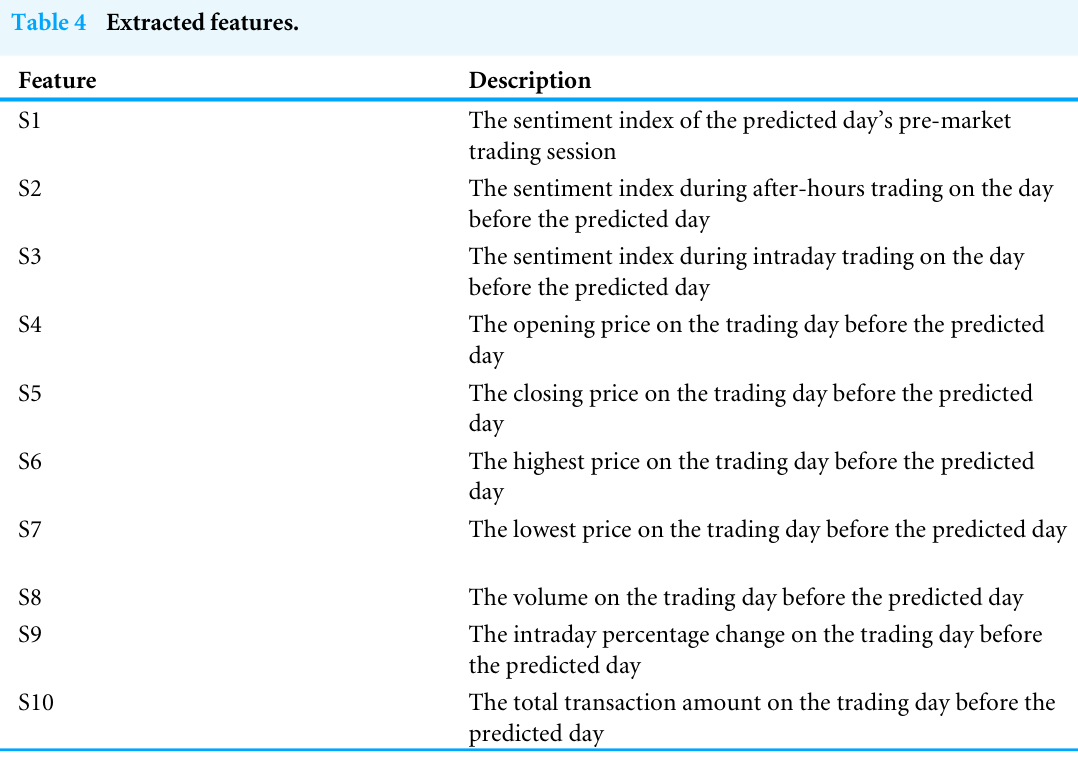
\includegraphics[width=0.95\linewidth]{gfx/m4l3_liu_table4_extracted_features.png}
\par\smallskip{\small \textbf{Bảng 4:} Các đặc trưng được trích xuất.}
\end{figure}

Chúng tôi đã sử dụng một máy vector hỗ trợ (SVM) tập hợp với bagging để xây dựng mô hình. Điều này đòi hỏi phải thiết lập các tham số cho cả bộ phân loại vector hỗ trợ (support vector classifier, SVC) và bộ phân loại bagging. SVC có một số siêu tham số quan trọng, chẳng hạn như hàm nhân, $C$ (tham số điều chuẩn hóa), và gamma (hệ số hàm nhân). Các tham số này được thể hiện chi tiết trong Bảng 5. Chúng tôi cũng đã sử dụng BaggingClassifier từ thư viện Python scikit-learn (Pedregosa và cộng sự, 2011). Bộ phân loại bagging có một số siêu tham số quan trọng cần được thiết lập, chẳng hạn như bộ ước lượng cơ sở (base estimator), số lượng bộ ước lượng (n\_estimators), và liệu các mẫu có được lấy có hoàn lại (bootstrap) hay không. Các tham số này được thể hiện chi tiết trong Bảng 6.

\begin{figure}[H]
\centering
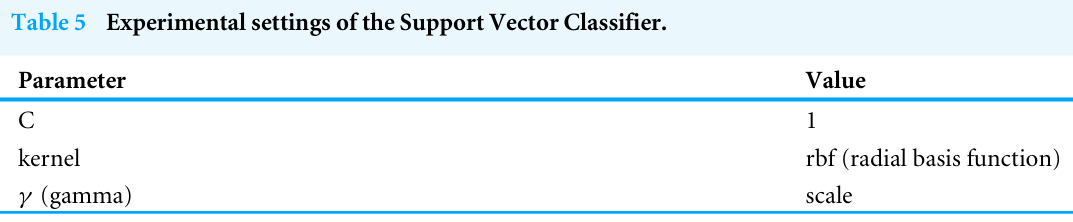
\includegraphics[width=0.8\linewidth]{gfx/m4l3_liu_table5_svc_settings.png}
\par\smallskip{\small \textbf{Bảng 5:} Thiết lập thực nghiệm của Bộ phân loại Vector Hỗ trợ (SVC).}
\end{figure}

\begin{figure}[H]
\centering
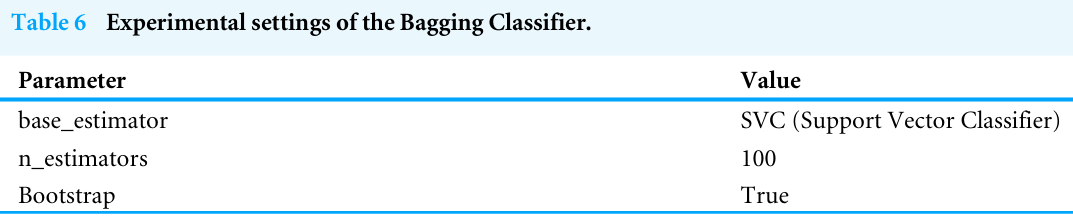
\includegraphics[width=0.8\linewidth]{gfx/m4l3_liu_table6_bagging_settings.png}
\par\smallskip{\small \textbf{Bảng 6:} Thiết lập thực nghiệm của Bộ phân loại Bagging.}
\end{figure}

\subsection*{Các chỉ số đánh giá}

Phương trình cho độ chính xác phân loại (classification accuracy) như sau, có thể biểu diễn tỷ lệ phần trăm của tổng số kết quả dự đoán đúng.

$$
\text{Accuracy} = \frac{\text{TP}+\text{TN}}{\text{TP}+\text{FP}+\text{FN}+\text{TN}}
$$

trong đó TP biểu thị giá trị dự đoán là 1 và giá trị thực cũng là 1; TN biểu thị giá trị dự đoán là 0 và giá trị thực cũng là 0; FP biểu thị giá trị dự đoán là 1 nhưng giá trị thực là 0; và FN biểu thị giá trị dự đoán là 0 nhưng giá trị thực là 1.

$$
\text{Precision} = \frac{\text{TP}}{\text{TP}+\text{FP}}
$$

trong đó độ chính xác (precision) là tỷ lệ phần trăm trong số các mẫu được dự đoán là giá cổ phiếu tăng mà giá thực tế thực sự đã tăng.

$$
\text{Recall} = \frac{\text{TP}}{\text{TP}+\text{FN}}
$$

trong đó độ bao phủ (recall) là tỷ lệ phần trăm trong số các mẫu thực tế có giá cổ phiếu tăng mà giá được dự đoán cũng tăng.

Trong việc dự đoán liệu giá cổ phiếu có tăng hay không, độ chính xác (precision) được coi là quan trọng hơn độ chính xác tổng thể (accuracy). Trong một thị trường tăng giá (bull market), cả độ chính xác (precision) và độ bao phủ (recall) đều quan trọng như nhau đối với việc ra quyết định. Tuy nhiên, trong một thị trường giảm giá (bear market), độ bao phủ (recall) trở nên quan trọng hơn độ chính xác (precision) vì nó có tác động lớn hơn đến khả năng thua lỗ tài chính tiềm ẩn (\url{http://www.bituzi.com/2019/10/confusionmatrix.html}).

$$
\text{F1 Score} = \frac{2 \cdot \text{Precision} \cdot \text{Recall}}{\text{Precision} + \text{Recall}}
$$

Điểm F1 (F1-score) ở trên là trung bình điều hòa (harmonic mean) của độ chính xác (precision) và độ bao phủ (recall). Điểm số bằng 1 đại diện cho hiệu suất cao nhất, và điểm số bằng 0 đại diện cho hiệu suất tệ nhất. Cả độ chính xác (precision) và độ bao phủ (recall) đều đóng góp như nhau vào điểm F1; do đó, điểm số càng gần 1 thì mô hình càng tốt (\url{https://scikit-learn.org/stable/modules/generated/sklearn.metrics.f1_score.html}). Do đó, đối với chủ đề này, chúng tôi đánh giá các phương pháp bằng điểm F1.

\section{Kết quả}

Trong nghiên cứu này, chúng tôi đã tiến hành năm thực nghiệm để đo lường hiệu suất của việc kết hợp các chỉ số cảm xúc trong dự đoán biến động giá cổ phiếu. Ngoài ra, thông qua các thực nghiệm này, chúng tôi có thể xác định liệu việc bổ sung cảm xúc có giúp mô hình dự báo biến động giá cổ phiếu hay không và so sánh hiệu suất của các phương pháp khác nhau để thu thập chỉ số cảm xúc. Các thực nghiệm (viết tắt là TN) như sau:
\begin{itemize}
  \item \textbf{TN 1.} Trong việc xây dựng mô hình, chỉ dữ liệu cổ phiếu lịch sử được sử dụng làm đặc trưng và không có dữ liệu cảm xúc nào được đưa vào xem xét. Do đó, chỉ các đặc trưng S4 đến S10 trong Bảng 4 được sử dụng trong mô hình.
  \item \textbf{TN 2.} Ngoài việc sử dụng dữ liệu cổ phiếu lịch sử, chúng tôi bổ sung các chỉ số cảm xúc được tính toán từ dữ liệu cảm xúc do người dùng cung cấp làm đặc trưng.
  \item \textbf{TN 3.} Để tăng tổng số lượng cảm xúc, không chỉ cảm xúc do người dùng cung cấp mà cả các bình luận không được gán nhãn cũng được phân loại là tăng giá hoặc giảm giá bằng một mô hình phân tích cảm xúc hai lớp. Chúng tôi sử dụng mô hình phân tích cảm xúc roberta-base-Stocktwits-finetuned (\url{https://huggingface.co/zhayunduo/roberta-base-Stocktwits-finetuned}) trong thực nghiệm này, đây là một mô hình phân tích cảm xúc được huấn luyện trên các bình luận Stocktwits và có thể đưa ra kết quả tăng giá hoặc giảm giá với độ chính xác 93.43\%.
  \item \textbf{TN 4.} Tất cả bình luận được gán nhãn bằng mô hình FinBERT, và các chỉ số cảm xúc được tính toán làm đặc trưng.
  \item \textbf{TN 5.} Tất cả bình luận được gán nhãn bằng mô hình VADER, và các chỉ số cảm xúc được tính toán làm đặc trưng, giống cách Koukaras, Nousi \& Tjortjis (2022) làm trong thực nghiệm tương tự với VADER. Mô hình cũng đưa ra ba lớp kết quả.
\end{itemize}

Theo Ren, Wu \& Liu (2019), việc lựa chọn ngẫu nhiên tập huấn luyện và tập kiểm định trong bộ dữ liệu của chúng tôi có thể dẫn đến thiên lệch nhìn trước. Ví dụ, chúng tôi dự đoán biến động giá cổ phiếu của ngày hôm nay, nhưng tập huấn luyện của chúng tôi chứa dữ liệu từ ngày mai và ngày kia, mang lại cho mô hình phân loại một lợi thế trước về xu hướng tương lai mà không thể đạt được trong các ứng dụng thực tế. Chúng tôi giải quyết vấn đề thiên lệch nhìn trước bằng cách sử dụng phương pháp cửa sổ trượt. Hình 8 minh họa ý tưởng này một cách đầy đủ. Để bắt đầu, cần xác định kích thước cửa sổ trượt phù hợp nhất cho mỗi thực nghiệm. Kích thước được xác định bằng cách huấn luyện trên các ngày trước đó, dự báo biến động của ngày tiếp theo cho đến cuối bộ dữ liệu, và chọn kích thước cửa sổ có độ chính xác cao nhất cho thực nghiệm. Khi chúng tôi đã chọn được kích thước tối ưu cho cửa sổ trượt, chúng tôi có thể sử dụng kích thước này vào tương lai để dự báo biến động giá của ngày mới. Kết quả là, chúng tôi huấn luyện và kiểm định mô hình bằng phương pháp cửa sổ trượt, cho phép chúng tôi tránh hiệu quả vấn đề thiên lệch nhìn trước và ngăn mô hình quá khớp với dữ liệu.

\begin{figure}[H]
\centering
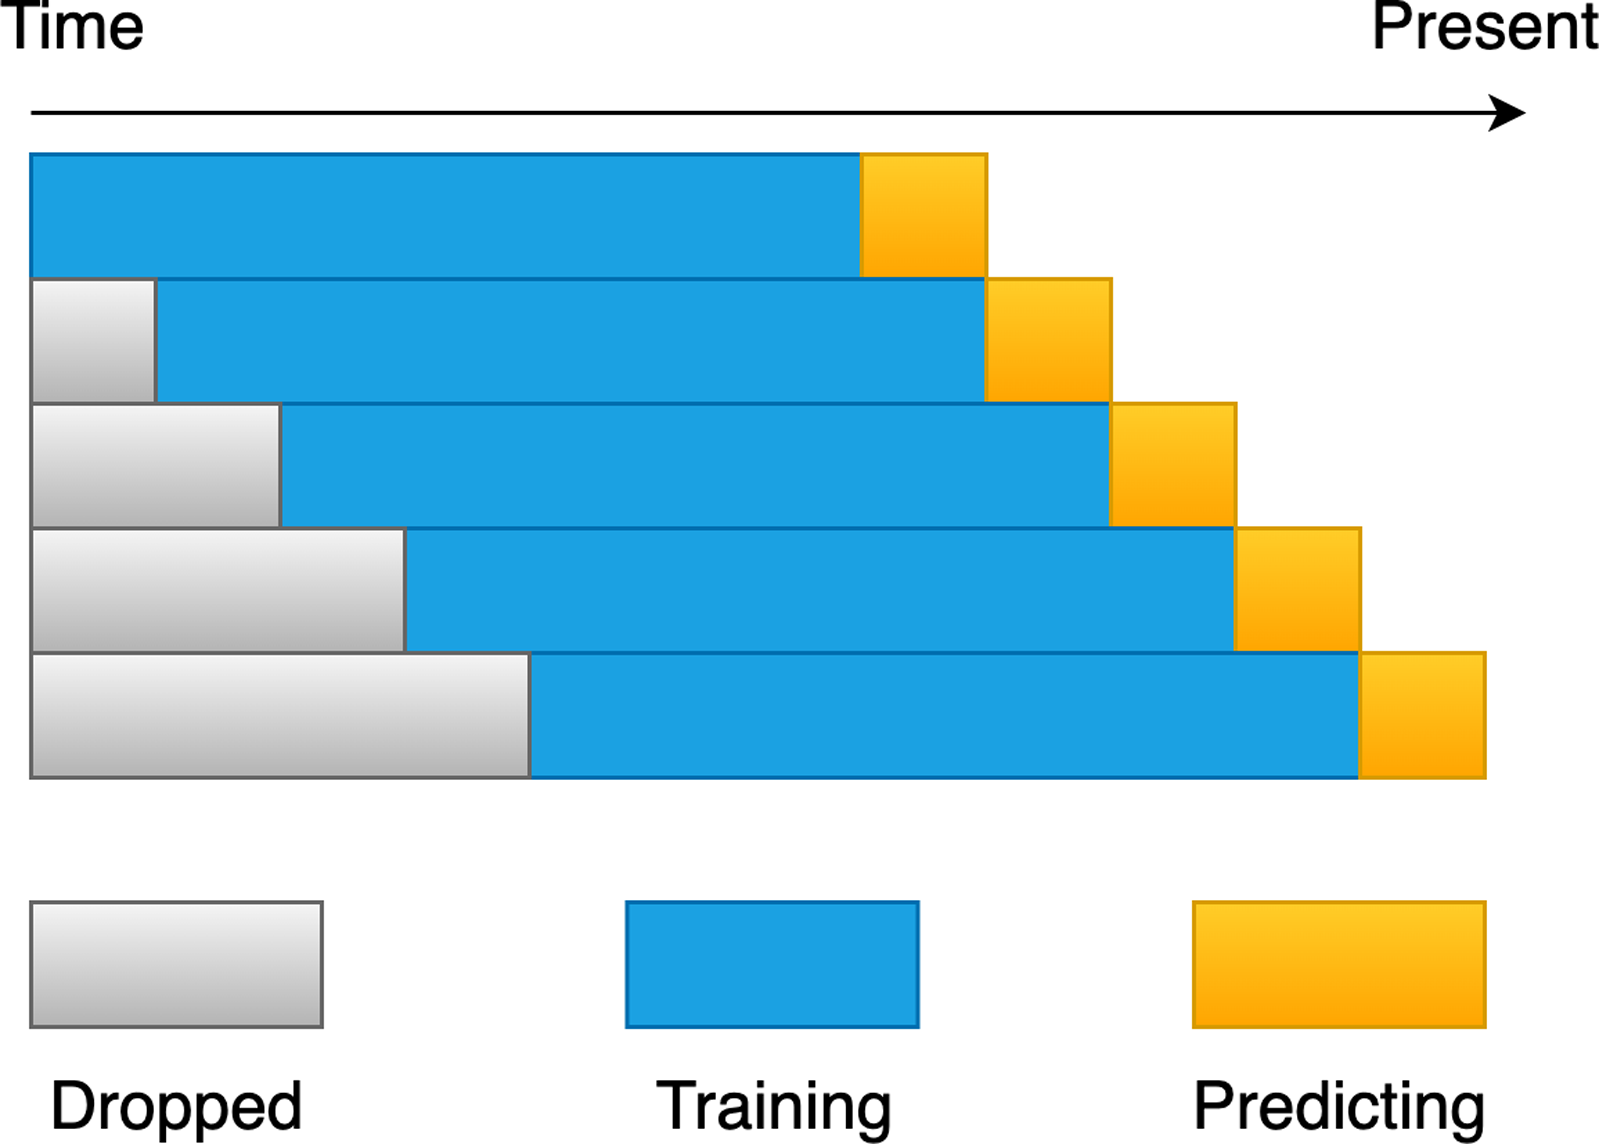
\includegraphics[width=0.6\linewidth]{gfx/m4l3_liu_fig8_rolling_window_procedure.png}
\par\smallskip{\small \textbf{Hình 8:} Sơ đồ biểu diễn quy trình cửa sổ trượt (rolling window).}
\end{figure}

Ngoài ra, chúng tôi tin rằng kích thước của cửa sổ trượt không nên quá nhỏ, vì điều kiện thị trường có thể thay đổi trong ngắn hạn. Ví dụ, nếu thị trường hiện đang tăng giá, một số yếu tố hoặc tin tức thị trường có thể khiến nó chuyển sang giảm giá. Nếu dữ liệu dùng để huấn luyện mô hình không đủ, ngay cả khi kết quả dự đoán tốt, khả năng tổng quát hóa của mô hình có thể kém hơn. Do đó, mặc dù bộ dữ liệu cho nghiên cứu này bị giới hạn, chúng tôi đặt kích thước huấn luyện của cửa sổ trượt trong khoảng từ 232 đến 252 (tương đương số ngày làm việc trong khoảng một năm), kích thước kiểm định của một cửa sổ là 1 cho mục đích thực nghiệm và phân tích, và kích thước cửa sổ huấn luyện được đặt là một số chia hết cho 2. Vì vậy, chúng tôi huấn luyện 11 mô hình dự đoán với các kích thước cửa sổ huấn luyện khác nhau trong mỗi thực nghiệm. Hơn nữa, do các điều kiện thị trường khác nhau giữa thị trường tăng giá và giảm giá, tập dữ liệu huấn luyện có thể mất cân bằng. Do đó, chúng tôi sử dụng SMOTE (Chawla và cộng sự, 2002), một kỹ thuật lấy mẫu quá mức (oversampling), để cân bằng dữ liệu huấn luyện.

Điểm F1 tốt nhất thu được từ kết quả thực nghiệm được trình bày trong Bảng 7.

\begin{figure}[H]
\centering
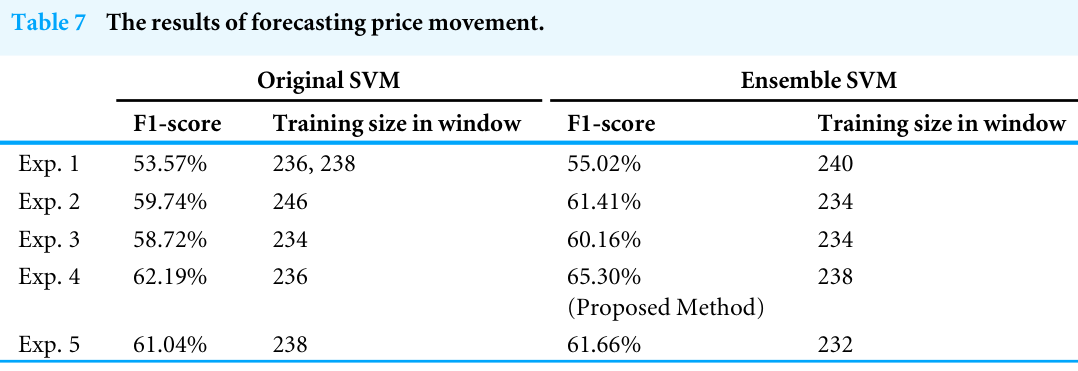
\includegraphics[width=0.95\linewidth]{gfx/m4l3_liu_table7_forecasting_results.png}
\par\smallskip{\small \textbf{Bảng 7:} Kết quả dự báo biến động giá.}
\end{figure}

Trong TN 1, việc thiếu các chỉ số cảm xúc dẫn đến kết quả kém chính xác hơn so với các thực nghiệm khác. Do đó, chúng tôi sử dụng kết quả của TN 1 làm cơ sở (baseline) cho các thực nghiệm còn lại.

Trong TN 2, việc bổ sung các cảm xúc được chủ động chỉ ra bởi người dùng cải thiện đáng kể hiệu suất của các dự đoán biến động giá cổ phiếu. Điều này chứng minh một mối tương quan mạnh mẽ giữa cảm xúc nhà đầu tư và biến động giá cổ phiếu.

Trong TN 3, chúng tôi đã sử dụng một mô hình phân tích cảm xúc hai lớp để tăng tổng lượng cảm xúc trong phân tích của chúng tôi. Tuy nhiên, chúng tôi phát hiện rằng một số bình luận không được gán nhãn liên quan đến chỉ trích về chính trị hoặc hoạt động của nền tảng. Những bình luận này không phù hợp để phân loại là tăng giá hoặc giảm giá, nhưng mô hình vẫn gán một nhãn do hạn chế của nó chỉ có thể đưa ra hai loại cảm xúc. Kết quả là, điểm F1 của dự báo giá cổ phiếu thấp hơn so với TN 2. Để khảo sát sâu hơn vấn đề này, chúng tôi đã chọn ngẫu nhiên 100 bình luận chưa được gán nhãn để gán nhãn thủ công và phát hiện rằng 45 trong số đó không phù hợp để được gán nhãn là tăng giá hoặc giảm giá. Những kết quả này chứng minh rằng việc sử dụng một mô hình phân tích cảm xúc hai lớp để thu thập thêm cảm xúc không nhất thiết cải thiện điểm F1 so với việc chỉ sử dụng các cảm xúc hai lớp do người dùng chủ động gán nhãn.

Trong TN 4, chúng tôi đã thu thập tất cả các bình luận về SPY trên Stocktwits trong hai năm qua và phân loại chúng bằng mô hình FinBERT, mô hình này cung cấp không chỉ cảm xúc tích cực và tiêu cực mà còn cả cảm xúc trung lập. Điều này giải quyết vấn đề của TN 3, nơi một mô hình phân tích cảm xúc hai lớp có thể phân loại một số bình luận không tăng giá và không giảm giá là tăng giá hoặc giảm giá. Tuy nhiên, FinBERT có khả năng phân loại các cảm xúc không liên quan đến tài chính là trung lập. Bằng cách tính toán công thức của chỉ số cảm xúc ba lớp được đề cập trong mục ``Phương pháp luận'', chúng tôi có thể phân biệt các bình luận không tăng giá hoặc không giảm giá về các chủ đề không liên quan đến tài chính, và các chỉ số cảm xúc hợp lý được thu được. Điểm F1 của phương pháp thay thế được đề xuất cao hơn các phương pháp khác.

Trong TN 5, chúng tôi đã sử dụng VADER làm mô hình phân tích cảm xúc, có khả năng đưa ra ba kết quả (tích cực, tiêu cực, và trung lập). Tuy nhiên, vì mô hình này không được thiết kế chuyên biệt cho lĩnh vực tài chính, hiệu suất của nó không vượt qua TN 4 (FinBERT).

\section{Thảo luận}

Hình 9 trình bày các biểu đồ tần suất điểm F1 (F1-score frequency histograms) cho mỗi thực nghiệm. Các biểu đồ cho thấy SVM tập hợp được triển khai cải thiện hiệu suất dự đoán biến động cổ phiếu trong tất cả các thực nghiệm. Bằng cách sử dụng kỹ thuật bagging, SVM tập hợp trong nghiên cứu này kết hợp các dự đoán từ nhiều bộ dự báo cơ sở, nắm bắt hiệu quả tính đa dạng của tập dữ liệu và nâng cao khả năng tổng quát hóa của mô hình. Cách tiếp cận này cũng giảm khả năng quá khớp so với việc sử dụng một bộ dự báo đơn lẻ, từ đó nâng cao độ chính xác. Kết quả tối ưu đạt được bằng phương pháp luận được đề xuất, sử dụng FinBERT để phân tích cảm xúc và SVM tập hợp cho dự đoán biến động giá cổ phiếu trong TN 4, đạt điểm F1 đỉnh là 65.30\%.

\begin{figure}[H]
\centering
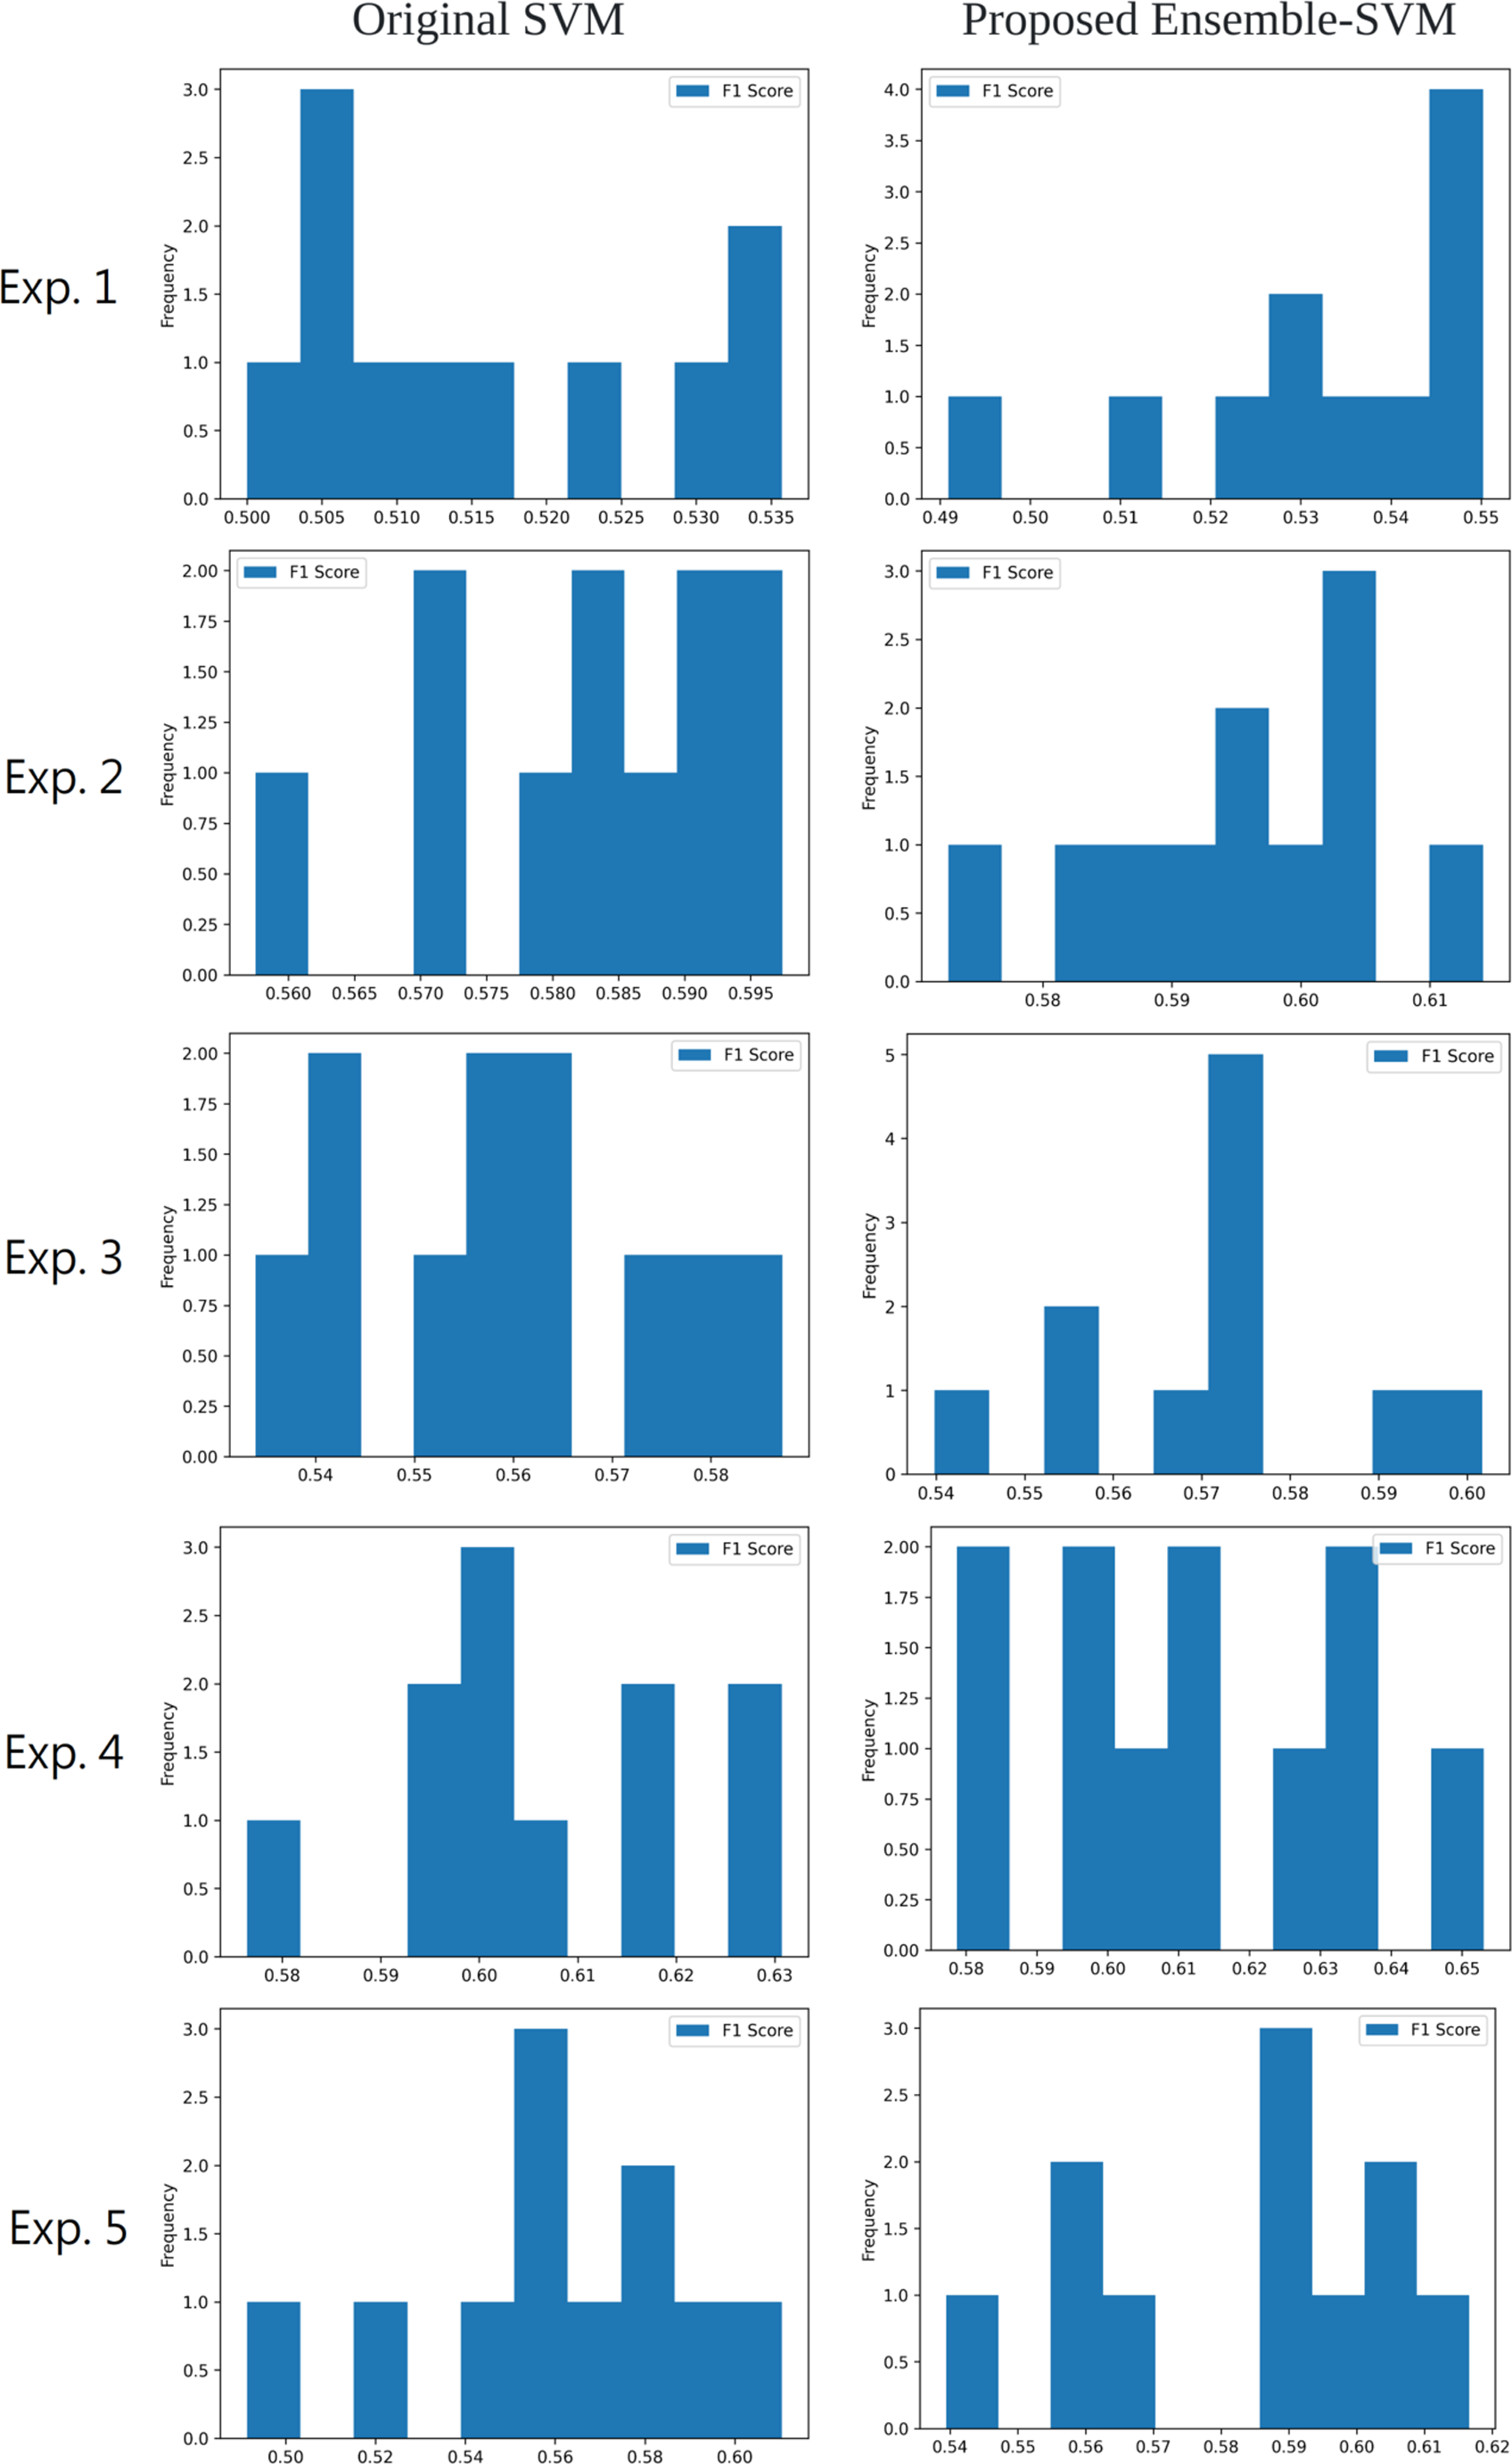
\includegraphics[width=0.85\linewidth]{gfx/m4l3_liu_fig9_f1score_histogram.png}
\par\smallskip{\small \textbf{Hình 9:} Biểu đồ tần suất của điểm F1 cho mỗi thực nghiệm.}
\end{figure}

Trong TN 1 và TN 2, chúng tôi so sánh mức cải thiện điểm F1 của dự đoán biến động giá cổ phiếu khi bổ sung cảm xúc nhà đầu tư. Vì Gupta \& Chen (2020) đã phát triển nhiều bộ phân tích cảm xúc hai lớp với độ chính xác khoảng 75 đến 85\%, và phân tích cảm xúc được theo sau bởi dự đoán biến động giá cổ phiếu, kết quả cho thấy nhiều bình luận hơn có hiệu quả trong việc cải thiện độ chính xác. Do đó, để so sánh với phương pháp này, chúng tôi đã sử dụng một bộ phân tích cảm xúc hai lớp với độ chính xác 93\% trong TN 3. Tuy nhiên, kết quả của dự đoán biến động giá cổ phiếu không đạt yêu cầu. Gupta \& Chen (2020) đề cập rằng một mô hình có cảm xúc trung lập có thể giảm nhiễu và cải thiện độ chính xác. Do đó, trong phương pháp của Koukaras, Nousi \& Tjortjis (2022), một mô hình có cảm xúc trung lập như VADER đã được sử dụng để phân tích, và kết quả tốt đã đạt được. Tuy nhiên, vì họ chỉ sử dụng 22 ngày trong tập kiểm định, chúng tôi không thể xác định khả năng tổng quát hóa của nó. Trong TN 5, chúng tôi đã sử dụng bộ dữ liệu của mình, lớn gấp hơn 10 lần so với bộ dữ liệu của họ, để dự đoán. Kết quả cho thấy cách tiếp cận này vượt trội hơn TN 3, nhưng không nhất thiết tốt hơn TN 2 (chỉ dự đoán dựa trên cảm xúc do người dùng chủ động gán nhãn). Trong TN 4, chúng tôi đề xuất một cách tiếp cận thay thế, đó là áp dụng mô hình FinBERT làm mô hình phân tích cảm xúc. Kết quả cho thấy cách tiếp cận này đạt được kết quả thực nghiệm tốt nhất.

\section{Kết luận}

Trong bài báo này, chúng tôi đề xuất một cách tiếp cận thay thế cho phân tích cảm xúc của bình luận Stocktwits nhằm dự đoán biến động giá cổ phiếu. Phương pháp được đề xuất của chúng tôi sử dụng mô hình FinBERT để giảm nhiễu, nâng cao mức độ vĩ mô và độ chính xác của các chỉ số cảm xúc, và giải quyết các lỗi phân loại phát sinh từ mô hình phân tích cảm xúc hai lớp. Bằng cách so sánh phương pháp của chúng tôi với các kỹ thuật được sử dụng trong các nghiên cứu trước đây, chúng tôi chứng minh tính hiệu quả của nó. Hơn nữa, chúng tôi giới thiệu một mô hình máy vector hỗ trợ tập hợp để cải thiện khả năng tổng quát hóa và tăng độ chính xác của các dự đoán biến động giá cổ phiếu. Chúng tôi cũng áp dụng phương pháp cửa sổ trượt để ngăn thiên lệch nhìn trước. Nhìn chung, nghiên cứu của chúng tôi đóng góp vào khối lượng nghiên cứu ngày càng tăng về dự đoán giá cổ phiếu dựa trên cảm xúc và có tiềm năng hỗ trợ nhà đầu tư đưa ra các quyết định sáng suốt.

Mặc dù đạt được độ chính xác lý tưởng trong việc dự đoán biến động giá cổ phiếu bằng phương pháp được đề xuất, vẫn còn những hạn chế khi chỉ dựa vào cảm xúc. Có thể xác định hai hướng chính để cải thiện trong tương lai. Thứ nhất, các phương pháp chỉ dựa vào cảm xúc mạng xã hội để dự đoán giá cổ phiếu dễ bị tổn thương trước sự thao túng có chủ đích, chẳng hạn như sự kiện ép bán khống (short squeeze) của GameStop năm 2021. Do đó, cần thiết phải thiết lập các cơ chế bảo vệ chống lại các thao túng như vậy trong tương lai. Thứ hai, hiệu suất của các phương pháp chỉ phụ thuộc vào cảm xúc mạng xã hội để dự đoán giá cổ phiếu là có giới hạn. Để nâng cao độ chính xác của dự đoán, chúng tôi dự định kết hợp phương pháp được đề xuất trong bài báo này với các chỉ báo phân tích kỹ thuật trong các nghiên cứu tương lai.

\section{Thông tin bổ sung và các công bố}

\subsection*{Tài trợ}

Nghiên cứu này được tài trợ bởi Chương trình Nghiên cứu Chung giữa Viện Công nghệ Kyushu và Đại học Khoa học và Công nghệ Quốc gia Đài Loan, theo khoản tài trợ Kyutech-NTUST-109-03. Bên tài trợ không có vai trò gì trong việc thiết kế nghiên cứu, thu thập và phân tích dữ liệu, quyết định công bố, hay việc chuẩn bị bản thảo.

\subsection*{Công bố tài trợ}

Các tác giả đã công bố thông tin tài trợ sau đây: Chương trình Nghiên cứu Chung giữa Viện Công nghệ Kyushu và Đại học Khoa học và Công nghệ Quốc gia Đài Loan: Kyutech-NTUST-109-03.

\subsection*{Xung đột lợi ích}

Các tác giả tuyên bố không có xung đột lợi ích nào.

\subsection*{Đóng góp của các tác giả}

\begin{itemize}
  \item Jin-Xian Liu đã hình thành và thiết kế các thí nghiệm, thực hiện các thí nghiệm, phân tích dữ liệu, thực hiện công việc tính toán, chuẩn bị các hình và/hoặc bảng, viết hoặc rà soát các bản thảo của bài báo, và phê duyệt bản thảo cuối cùng.
  \item Jenq-Shiou Leu đã hình thành và thiết kế các thí nghiệm, phân tích dữ liệu, viết hoặc rà soát các bản thảo của bài báo, và phê duyệt bản thảo cuối cùng.
  \item Stefan Holst đã hình thành và thiết kế các thí nghiệm, phân tích dữ liệu, viết hoặc rà soát các bản thảo của bài báo, và phê duyệt bản thảo cuối cùng.
\end{itemize}

\subsection*{Khả năng tiếp cận dữ liệu}

Dữ liệu phân tích cảm xúc, dữ liệu thực nghiệm, và dữ liệu lịch sử giá cổ phiếu được cung cấp trong các Tệp Bổ sung (Supplemental Files). Bộ dữ liệu tin nhắn SPY có sẵn tại Figshare: Liu, Jin-Xian (2022): SPY\_stocktwits\_messages.csv. figshare. Dataset. \url{https://doi.org/10.6084/m9.figshare.20237736.v1}.

\subsection*{Thông tin bổ sung}

Thông tin bổ sung cho bài báo này có thể được tìm thấy trực tuyến tại \url{http://dx.doi.org/10.7717/peerj-cs.1403#supplemental-information}.

% [Đã lược bỏ danh mục Tài liệu tham khảo gốc (tiếng Anh, trích dẫn của tác giả bài gốc) để giảm dung lượng chương; không ảnh hưởng nội dung học thuật chính.]


% ---- Lesson 4: KHÔNG có Required Reading (WQU không yêu cầu đọc thêm) ----
\chapter{Mạng Xã hội}
\label{ch:M4L4}

% Lesson: Social Media

\section*{Lesson Notes}

MODULE 4 | BÀI 4

{\small
\begin{longtable}{>{\raggedright\arraybackslash}p{0.213\linewidth}>{\raggedright\arraybackslash}p{0.727\linewidth}}
\toprule
\textbf{Thời gian đọc} & 6 giờ \\
\addlinespace[2pt]
\textbf{Kiến thức nền tảng} & API, chức năng của mạng xã hội nói chung \\
\addlinespace[2pt]
\textbf{Từ khóa} & API, youtube, reddit, subreddit, phân tích cảm xúc, nltk, từ khóa \\
\addlinespace[2pt]
\bottomrule
\end{longtable}
}

\emph{Mạng xã hội đã trở thành một phần không thể tách rời của đời sống hiện đại, làm thay đổi cách chúng ta giao tiếp, chia sẻ thông tin và tương tác với thế giới xung quanh. Để hiểu tầm quan trọng của dữ liệu mạng xã hội và các ứng dụng của nó ngày nay, cần thiết phải xem xét quá trình phát triển lịch sử của các nền tảng này.}

\emph{Nguồn gốc của mạng xã hội có thể truy ngược về những ngày đầu của internet. Năm 1997, SixDegrees.com ra mắt như trang mạng xã hội đầu tiên có thể nhận diện được, cho phép người dùng tạo hồ sơ và liệt kê bạn bè. Điều này mở đường cho các nền tảng về sau như Friendster, MySpace, và cuối cùng là Facebook, nền tảng đã làm cách mạng hóa bức tranh mạng xã hội. Khi các nền tảng này ngày càng phổ biến và giàu chức năng, chúng bắt đầu tạo ra lượng dữ liệu người dùng khổng lồ. Dữ liệu này, bao gồm mọi thứ từ hồ sơ và kết nối của người dùng đến các tương tác với nội dung và các khuôn mẫu hành vi, nhanh chóng trở thành nguồn tài nguyên quý giá cho các nhà nghiên cứu, nhà tiếp thị và doanh nghiệp.}

\emph{Sự trỗi dậy của dữ liệu mạng xã hội như một lĩnh vực nghiên cứu và ứng dụng diễn ra đồng thời với mức độ tinh vi ngày càng tăng của các nền tảng này. Chẳng hạn, việc Facebook giới thiệu News Feed vào năm 2006 không chỉ thay đổi cách người dùng tương tác với nền tảng mà còn cung cấp một nguồn dữ liệu phong phú về sở thích và hành vi của người dùng. Ngày nay, dữ liệu mạng xã hội được sử dụng trong nhiều lĩnh vực, bao gồm tiếp thị, y tế công cộng, khoa học chính trị và nghiên cứu xã hội. Các nền tảng như YouTube và Reddit mang lại những hiểu biết độc đáo về hành vi người dùng, việc tiêu thụ nội dung và diễn ngôn công chúng. Thông qua các API (giao diện lập trình ứng dụng, application programming interface) do các nền tảng này cung cấp, các nhà nghiên cứu và nhà phát triển có thể truy cập và phân tích dữ liệu này theo những cách chưa từng có.}

\emph{Trong bài học này, chúng ta sẽ tập trung vào các khía cạnh thực hành của việc truy xuất và làm việc với dữ liệu mạng xã hội. Chúng ta sẽ khám phá cách sử dụng API để thu thập dữ liệu từ YouTube và Reddit, qua đó minh họa các ứng dụng thực tế của việc phân tích dữ liệu mạng xã hội. Bằng cách hiểu cả bối cảnh lịch sử lẫn các phương pháp hiện hành, chúng ta có thể đánh giá đúng hơn sức mạnh và tiềm năng của dữ liệu mạng xã hội trong bối cảnh số ngày nay.}

\section{Mạng Xã hội là gì?}

Chúng ta sẽ đưa ra một số định nghĩa về mạng xã hội là gì, dù có lẽ mỗi người trong chúng ta đều đã tiếp xúc đủ nhiều với các nền tảng như vậy.

Boyd và Ellison định nghĩa các trang mạng xã hội là những dịch vụ dựa trên web cho phép cá nhân
\begin{itemize}
  \item xây dựng một hồ sơ công khai hoặc bán công khai trong một hệ thống có giới hạn,
  \item lập danh sách những người dùng khác mà họ có kết nối, và
  \item xem và duyệt qua danh sách kết nối của mình cũng như của những người khác trong hệ thống.
\end{itemize}
Thông tin này làm nổi bật các khía cạnh cấu trúc của mạng xã hội, chẳng hạn hồ sơ người dùng, các kết nối và khả năng hiển thị của mạng lưới.

Định nghĩa trong Từ điển Merriam-Webster nhấn mạnh các khía cạnh giao tiếp và xây dựng cộng đồng của mạng xã hội: các mạng xã hội là những hình thức giao tiếp điện tử (chẳng hạn các trang web dành cho mạng xã hội và tiểu blog, microblogging) thông qua đó người dùng tạo ra các cộng đồng trực tuyến để chia sẻ thông tin, ý tưởng, tin nhắn cá nhân và các nội dung khác (chẳng hạn video) (``Social media'' [\emph{Merriam-Webster.com Dictionary}]).

Mặt khác, Từ điển Cambridge mô tả mạng xã hội như các nền tảng công nghệ: các trang web và chương trình máy tính cho phép mọi người giao tiếp và chia sẻ thông tin trên internet bằng máy tính hoặc điện thoại di động (``Social media'' [\emph{Cambridge Dictionary}]).

Tóm lại, chúng ta có thể tổng hợp các khía cạnh của mạng xã hội như sau:
\begin{itemize}
  \item Hồ sơ và kết nối của người dùng
  \item Cộng đồng trực tuyến
  \item Chia sẻ thông tin và nội dung
  \item Nền tảng công nghệ
  \item Nội dung do người dùng tạo ra
  \item Tính tương tác và cộng tác
  \item Mạng lưới ảo
  \item Biểu đạt và giao tiếp
\end{itemize}

Mỗi đặc điểm trên đều là một quá trình tạo ra dữ liệu. Chẳng hạn, phần ``Hồ sơ và kết nối của người dùng'' của mạng xã hội tạo ra dữ liệu nhân khẩu học, bản thân mạng xã hội (bạn bè, người theo dõi và các kết nối), cùng sở thích và ưu tiên cá nhân. Phần ``Cộng đồng trực tuyến'' tạo ra dữ liệu về tư cách thành viên nhóm, các khuôn mẫu tương tác trong cộng đồng, và các mối quan tâm/xu hướng trong những cộng đồng khác nhau.

Đến đây có thể thấy rõ rằng lượng dữ liệu khổng lồ được tạo ra có thể được dùng cho nhiều mục đích tùy thuộc vào mục tiêu của nhà nghiên cứu. Cụ thể, trong bối cảnh tài chính, chúng ta đặc biệt quan tâm đến ``Nội dung do người dùng tạo ra'', từ đó có thể trích xuất:
\begin{itemize}
  \item dữ liệu văn bản: bài đăng, bình luận
  \item dữ liệu cảm xúc và quan điểm
  \item nội dung đa phương tiện liên quan đến các chủ đề tài chính
\end{itemize}

Dữ liệu này có giá trị đối với một số ứng dụng đặc thù của tài chính:

\begin{itemize}
  \item Phân tích cảm xúc thị trường: Bằng cách phân tích cảm xúc của các bài đăng trên mạng xã hội về các cổ phiếu, hàng hóa, điều kiện thị trường cụ thể, v.v., các nhà nghiên cứu có thể lượng hóa ý kiến công chúng.
  \item Dự đoán giá cổ phiếu: Một số nghiên cứu đã cho thấy mối tương quan giữa cảm xúc trên mạng xã hội và các thay đổi giá cổ phiếu ngắn hạn, khiến dữ liệu này có khả năng hữu ích cho các chiến lược giao dịch.
  \item Phổ biến tin tức tài chính: Mạng xã hội thường lan truyền tin tức tài chính nhanh hơn các phương tiện truyền thông truyền thống!
  \item Đánh giá rủi ro: Bằng cách theo dõi các cuộc thảo luận trên mạng xã hội, các tổ chức tài chính có thể sớm nhận diện các rủi ro tiềm tàng hoặc các vấn đề về danh tiếng.
  \item Xu hướng tiền mã hóa: Do vai trò đáng kể của các cộng đồng trực tuyến trong thị trường tiền mã hóa, dữ liệu mạng xã hội đặc biệt có giá trị trong lĩnh vực này.
\end{itemize}

\section{Truy xuất Dữ liệu}

Trong phần này, chúng ta sẽ đưa ra một số ví dụ về cách sử dụng API để kết nối với một nền tảng mạng xã hội, cách truy xuất dữ liệu, và dữ liệu trông như thế nào trước khi được cấu trúc hóa thành các dataframe để vẽ biểu đồ và phân tích.

\subsection{Một Ví dụ về Lượng hóa Cảm xúc bằng Dữ liệu YouTube}

Trong tiểu mục này, chúng ta sẽ khám phá cách tận dụng YouTube API để thu thập và phân tích cảm xúc công chúng xoay quanh các sự kiện tài chính quan trọng. Chúng ta sẽ dùng đợt sụp đổ thị trường năm 2020 làm nghiên cứu tình huống để hiểu cách cảm xúc có thể được lượng hóa và tương quan với dữ liệu tài chính như chỉ số S\&P 500.

Điều kiện tiên quyết:

\begin{itemize}
  \item Tài khoản Google: Hãy bảo đảm bạn có một tài khoản Google đang hoạt động. Điều này cần thiết để truy cập các dịch vụ API của Google.

  \item Dự án Google Cloud: Bạn cần tạo một dự án trong Google Cloud Console. Dự án này sẽ lưu trữ khóa API của bạn, vốn thiết yếu để truy cập dữ liệu của YouTube.
\end{itemize}

Thiết lập YouTube API: Thực hiện các bước sau để bắt đầu:

\begin{enumerate}
  \item Truy cập Google Cloud Console.

  \item Tạo một dự án mới.

  \item Điều hướng đến API Library và bật YouTube Data API v3.

  \item Tạo thông tin xác thực (khóa API) để truy cập API.
\end{enumerate}

\begin{lstlisting}[language=Python,escapeinside={(*@}{@*)}]
import requests
import praw
from datetime import datetime, timedelta
import matplotlib.pyplot as plt
import pandas as pd
from collections import defaultdict
from googleapiclient.discovery import build
from googleapiclient.errors import HttpError
import yfinance as yf
import seaborn as sns
sns.set()
\end{lstlisting}

Những Lưu ý Chính

\begin{enumerate}
  \item Quản lý Hạn ngạch: Hãy lưu ý các giới hạn hạn ngạch của API. Google cung cấp miễn phí một số lượng yêu cầu hạn chế mỗi ngày. Hãy lập kế hoạch truy xuất dữ liệu cẩn thận để nằm trong các giới hạn này, nếu không bạn sẽ buộc phải dừng quy trình làm việc trong một ngày.

  \item Lựa chọn Từ khóa: Việc chọn từ khóa là then chốt. Hãy nghĩ về những thuật ngữ có liên quan vào thời điểm diễn ra sự kiện tài chính. Trong nghiên cứu tình huống về cuộc sụp đổ năm 2020, chúng tôi đã dùng các thuật ngữ như ``recession'', ``economic crisis'', ``inflation'', v.v.

  \item Lựa chọn Kênh: Hãy chọn các kênh uy tín và phù hợp, cung cấp nội dung nhất quán và chất lượng cao.

  \item Phân tích Dữ liệu: Sau khi truy xuất dữ liệu, bạn sẽ phân tích tần suất của các từ khóa và đối chiếu nó với các chỉ số tài chính như chỉ số S\&P 500.
\end{enumerate}

\begin{lstlisting}[language=Python,escapeinside={(*@}{@*)}]
API_KEY = "YOUR_API_KEY"
CHANNEL_NAMES = ['cnbc'] # (*@Bạn@*) (*@có@*) (*@thể@*) (*@đưa@*) (*@vào@*) (*@các@*) (*@kênh@*) (*@tài@*) (*@chính@*) (*@YouTube@*) (*@do@*) (*@bạn@*) (*@chọn@*)
CHANNEL_IDs = {} # (*@Từ@*) (*@điển@*) (*@lưu@*) (*@tên@*) (*@kênh@*) (*@và@*) (*@ID@*) (*@của@*) (*@chúng@*)

# (*@Hàm@*) (*@lấy@*) (*@ID@*) (*@kênh@*) (*@theo@*) (*@tên@*) (*@kênh@*)
def get_channel_id_by_name(channel_name, api_key):
    url = f"https://www.googleapis.com/youtube/v3/search?part=snippet&type=channel&q={channel_name}&key={api_key}"
    response = requests.get(url)
    data = response.json()
    return data['items'][0]['snippet']['channelId']

# (*@Lấy@*) (*@ID@*) (*@kênh@*) (*@cho@*) (*@tất@*) (*@cả@*) (*@tên@*) (*@kênh@*)
for channel_name in CHANNEL_NAMES:
    channel_id = get_channel_id_by_name(channel_name, API_KEY)
    CHANNEL_IDs[channel_name] = channel_id

# (*@In@*) (*@tên@*) (*@các@*) (*@kênh@*) (*@và@*) (*@ID@*) (*@của@*) (*@chúng@*)
for channel_name, channel_id in CHANNEL_IDs.items():
    print(f"{channel_name}: {channel_id}")
\end{lstlisting}

\begin{lstlisting}[language=Python,escapeinside={(*@}{@*)}]
# (*@Định@*) (*@nghĩa@*) (*@các@*) (*@tham@*) (*@số@*)
KEYWORDS = ['recession', 'unemployment', 'crash', 'stimulus', 'crisis', 'inflation'] # (*@Danh@*) (*@sách@*) (*@các@*) (*@từ@*) (*@khóa@*) (*@cần@*) (*@tìm@*). (*@Bạn@*) (*@có@*) (*@thể@*) (*@đưa@*) (*@vào@*) (*@các@*) (*@từ@*) (*@khóa@*) (*@liên@*) (*@quan@*) (*@do@*) (*@bạn@*) (*@chọn@*)
START_DATE = '2020-01-01T00:00:00Z'
END_DATE = '2020-05-30T23:59:59Z'
\end{lstlisting}

\begin{lstlisting}[language=Python,escapeinside={(*@}{@*)}]
# (*@Khởi@*) (*@tạo@*) (*@YouTube@*) (*@API@*)
def initialize_youtube(api_key):
    youtube = build('youtube', 'v3', developerKey=api_key)
    return youtube

# (*@Lấy@*) (*@các@*) (*@video@*) (*@từ@*) (*@một@*) (*@kênh@*)
def get_videos(youtube, channel_id, start_date, end_date):
    request = youtube.search().list(
        part='snippet',
        channelId=channel_id,
        publishedAfter=start_date,
        publishedBefore=end_date,
        maxResults=50,
        type='video'
    )
    videos = []
    while request:
        response = request.execute()
        videos.extend(response['items'])
        request = youtube.search().list_next(request, response)
    return videos

# (*@Lấy@*) (*@các@*) (*@bình@*) (*@luận@*) (*@từ@*) (*@một@*) (*@video@*)
def get_comments(youtube, video_id):
    comments = []
    request = youtube.commentThreads().list(
        part='snippet',
        videoId=video_id,
        maxResults=100
    )
    while request:
        try:
            response = request.execute()
            comments.extend(response['items'])
            request = youtube.commentThreads().list_next(request, response)
        except HttpError as e:
            if e.resp.status == 403 and 'commentsDisabled' in str(e):
                print(f"Comments are disabled for video ID: {video_id}")
                break
            else:
                raise e
    return comments

# (*@Lọc@*) (*@dữ@*) (*@liệu@*) (*@và@*) (*@đếm@*) (*@số@*) (*@lần@*) (*@nhắc@*) (*@đến@*) (*@từ@*) (*@khóa@*)
def filter_and_count_comments(comments, keywords, start_date, end_date):
    keyword_counts = defaultdict(int)
    start = datetime.strptime(start_date, '%Y-%m-%dT%H:%M:%SZ')
    end = datetime.strptime(end_date, '%Y-%m-%dT%H:%M:%SZ')
    current_date = start

    while current_date <= end:
        keyword_counts[current_date.strftime('%Y-%m-%d')] = 0
        current_date += timedelta(days=1)

    for comment_thread in comments:
        comment = comment_thread['snippet']['topLevelComment']['snippet']
        comment_date = datetime.strptime(comment['publishedAt'], '%Y-%m-%dT%H:%M:%SZ').strftime('%Y-%m-%d')
        comment_text = comment['textDisplay'].lower()
        if any(keyword in comment_text for keyword in keywords):
            keyword_counts[comment_date] += 1

    return keyword_counts

def plot_keyword_counts(keyword_counts, channel_name):
    dates = list(keyword_counts.keys())
    counts = list(keyword_counts.values())
    df = pd.DataFrame({'Date': dates, 'Count': counts})
    df['Date'] = pd.to_datetime(df['Date'])
    df = df.set_index('Date')
    df.sort_index(inplace=True)

    plt.figure(figsize=(14, 7))  # (*@Điều@*) (*@chỉnh@*) (*@kích@*) (*@thước@*) (*@hình@*) (*@để@*) (*@dễ@*) (*@đọc@*) (*@hơn@*)
    ax = df.plot(kind='bar', legend=False, width = 0.8)
    ax.set_title(f'Keyword Mentions per Day in {channel_name}')
    ax.set_xlabel('Date')
    ax.set_ylabel('Count of Keywords')

    # (*@Đặt@*) (*@các@*) (*@vạch@*) (*@chia@*) (*@trục@*) (*@x@*) (*@theo@*) (*@khoảng@*) (*@đều@*) (*@và@*) (*@xoay@*) (*@nhãn@*) (*@để@*) (*@dễ@*) (*@đọc@*) (*@hơn@*)
    ax.set_xticks(range(0, len(df.index), 14))
    ax.set_xticklabels(df.index.strftime('%Y-%m-%d')[::14], rotation=45, ha='right')

    #plt.tight_layout()
    plt.show()
\end{lstlisting}

\begin{lstlisting}[language=Python,escapeinside={(*@}{@*)}]
# (*@Kịch@*) (*@bản@*) (*@chính@*)
# (*@Ô@*) (*@NÀY@*) (*@CÓ@*) (*@THỂ@*) (*@MẤT@*) (*@NHIỀU@*) (*@THỜI@*) (*@GIAN@*) (*@ĐỂ@*) (*@HOÀN@*) (*@THÀNH@*), (*@THẬM@*) (*@CHÍ@*) (*@GẦN@*) (*@20@*) (*@PHÚT@*).
# (*@XIN@*) (*@HÃY@*) (*@KIÊN@*) (*@NHẪN@*).

# (*@Khởi@*) (*@tạo@*) (*@client@*) (*@YouTube@*) (*@API@*)
youtube = initialize_youtube(API_KEY)

# (*@Lấy@*) (*@các@*) (*@video@*) (*@từ@*) (*@kênh@*) (*@được@*) (*@chỉ@*) (*@định@*) (*@trong@*) (*@khoảng@*) (*@ngày@*) (*@đã@*) (*@cho@*)
videos = get_videos(youtube, channel_id, START_DATE, END_DATE)

# (*@Khởi@*) (*@tạo@*) (*@một@*) (*@danh@*) (*@sách@*) (*@để@*) (*@lưu@*) (*@tất@*) (*@cả@*) (*@bình@*) (*@luận@*)
all_comments = []

# (*@Lấy@*) (*@bình@*) (*@luận@*) (*@cho@*) (*@từng@*) (*@video@*)
for video in videos:
    video_id = video['id']['videoId']
    try:
        comments = get_comments(youtube, video_id)
        all_comments.extend(comments)
    except HttpError as e:
        print(f"An error occurred: {e}")

# (*@Lọc@*) (*@và@*) (*@đếm@*) (*@từ@*) (*@khóa@*) (*@trong@*) (*@các@*) (*@bình@*) (*@luận@*)
keyword_counts = filter_and_count_comments(all_comments, KEYWORDS, START_DATE, END_DATE)
\end{lstlisting}

Ở ô bên dưới, bạn có thể thấy một phản hồi trông như thế nào. Bạn có thể dùng trí tưởng tượng để nghĩ xem dữ liệu có thể được sử dụng ra sao. Chẳng hạn, khóa \texttt{likeCount} có thể được dùng để đánh giá liệu một bình luận cụ thể có nên được gán trọng số cao hơn các bình luận còn lại hay không. Các giá trị \texttt{totalReplyCount} có thể được dùng để nhận diện các chủ đề gây tranh cãi, được yêu thích hoặc thú vị.

\begin{lstlisting}[language=Python,escapeinside={(*@}{@*)}]
comments[0]
\end{lstlisting}

\begin{lstlisting}[language=Python,escapeinside={(*@}{@*)}]
# (*@Chuẩn@*) (*@bị@*) (*@tập@*) (*@dữ@*) (*@liệu@*) (*@để@*) (*@trực@*) (*@quan@*) (*@hóa@*)
df_keywords = pd.DataFrame(keyword_counts.items()).set_index(0)
df_keywords.index = pd.to_datetime(df_keywords.index)
df_keywords.sort_index(inplace=True)
df_keywords.columns = ['count']
df_keywords['count'] = df_keywords['count'].astype(int)
df_keywords = df_keywords.resample('D').sum()

rolling_sum = df_keywords.loc[:"2020-05-30"].rolling('7D').sum()

# (*@Tải@*) (*@S\&P500@*) (*@làm@*) (*@chuẩn@*) (*@so@*) (*@sánh@*)
gspc = yf.download('^GSPC', start='2020-01-01', end='2020-05-30')['Adj Close']

# (*@Vẽ@*) (*@biểu@*) (*@đồ@*)
fig, ax1 = plt.subplots(figsize=(16, 7))

# (*@Vẽ@*) (*@dữ@*) (*@liệu@*) (*@từ@*) (*@khóa@*)
#ax1.plot(df_keywords.loc[:"2020-05-30"].rolling('7D').sum(), color='green', alpha=0.6, label='Rolling weekly sum of keywords')
ax1.bar(rolling_sum.index, rolling_sum.values.flatten(), color='green', alpha=0.6, label='Rolling weekly sum of keywords')
#ax1.set_ylim(-1, 40)
ax1.set_ylabel('Sum of Keywords')

# (*@Tạo@*) (*@trục@*) (*@kép@*) (*@để@*) (*@vẽ@*) (*@dữ@*) (*@liệu@*) (*@S\&P500@*)
ax2 = ax1.twinx()
ax2.plot(gspc, color='blue', alpha=0.5, label='S&P500 Price')
ax2.set_ylim(1500, 3400)
ax2.set_ylabel('S&P500 Price')

# (*@Thêm@*) (*@chú@*) (*@giải@*)
ax1.legend(loc='upper left')
ax2.legend(loc='upper right')

plt.title('Rolling weekly sum of keywords and S&P500 Price')
plt.show()
\end{lstlisting}

Đồ thị trên là một ví dụ về cách lượng hóa cảm xúc. Cách dễ nhất là đếm số lượng từ do ta chọn, và vì một số từ không dễ xuất hiện trừ khi có lý do, ta có thể tin rằng việc nhắc đến những từ đó vượt mức thông thường cho thấy cảm xúc tại thời điểm đó. Các thanh màu xanh lá biểu diễn tổng số từ khóa như ``recession'', ``economic crisis'' và ``inflation'' tìm thấy trong các bình luận YouTube, cho thấy mối quan ngại của công chúng gia tăng. Đường màu xanh dương theo dõi giá chỉ số S\&P 500, làm nổi bật phản ứng của thị trường trong cùng giai đoạn. Khi số lần nhắc đến từ khóa tiếp tục tăng sau tháng 3 năm 2020, trùng với đợt giảm mạnh của S\&P 500, ta quan sát thấy mối quan ngại ngày càng tăng của người dân và tác động của đợt sụp đổ lên cảm xúc chung.

\textbf{Bài tập 1}

Hãy chọn một tài sản và một giai đoạn mà các sự kiện quan trọng đối với tài sản đó đã xảy ra. Xác định các từ khóa bạn muốn đếm và (các) kênh phù hợp cho phân tích của bạn. Sử dụng đoạn mã đã cung cấp và thực hiện cùng quy trình như trên. Vẽ biểu đồ kết quả (bạn có thể phải chỉnh sửa mã đáng kể) và đăng lên diễn đàn cùng với phần phân tích ``chúng ta thấy gì''.

\subsection{Reddit}

Reddit là một trang web tin tức xã hội và thảo luận phổ biến, nơi người dùng có thể chia sẻ nội dung và tham gia các cuộc trò chuyện về nhiều chủ đề khác nhau, bao gồm tiền mã hóa. Đối với sinh viên ngành kỹ thuật tài chính, dữ liệu Reddit có thể cung cấp những ví dụ giá trị về cách thu được hiểu biết sâu sắc về cảm xúc và xu hướng thị trường.

Trong phần này, chúng ta sẽ khám phá cách sử dụng Reddit API để thu thập và phân tích dữ liệu liên quan đến các cuộc thảo luận về tiền mã hóa. Reddit API cho phép các nhà phát triển truy cập cơ sở dữ liệu của Reddit gồm các bài đăng, bình luận và nội dung khác một cách có lập trình. Để sử dụng API, bạn cần tạo một tài khoản Reddit và đăng ký một ứng dụng để nhận các thông tin xác thực cần thiết (client ID, client secret và user agent). Ở bước này, bạn được khuyến nghị sử dụng các hướng dẫn từ AI để hoàn thành.

Ví dụ của chúng ta tập trung vào việc phân tích cảm xúc trong các subreddit liên quan đến tiền mã hóa trong tháng vừa qua. Điều này là do các hạn chế của API Reddit và do nó không được tạo ra để phân tích dữ liệu mà chỉ là một công cụ dành cho những người điều hành subreddit. Đoạn mã chỉ xét tháng gần nhất (tháng gần nhất tính từ thời điểm bạn chạy các ô mã), và vì lý do này, kết quả được kỳ vọng sẽ khác nhau mỗi lần bạn chạy mã.

Bạn được KHUYẾN CÁO MẠNH không được chạy liên tục ô tải bình luận, vì ứng dụng của bạn sẽ bị hạn chế truy cập các subreddit này, dù điều đó có thể được khắc phục bằng cách tạo một ứng dụng mới. Đây là lời nhắc nhở cho sinh viên rằng dữ liệu phân tích cảm xúc không miễn phí. Chúng ta bị ràng buộc bởi các hạn chế của API và sự thiếu vắng dữ liệu lịch sử miễn phí.

Cũng cần lưu ý rằng dù ta thường kỳ vọng phân tích cảm xúc sẽ khớp sát với biến động giá, mối tương quan này không phải lúc nào cũng hoàn hảo. Các yếu tố như thao túng thị trường, tin tức bên ngoài hoặc thay đổi về quy định có thể gây ra sự phân kỳ giữa cảm xúc và giá. Tuy nhiên, phân tích cảm xúc vẫn là một công cụ có giá trị để hiểu tâm lý thị trường và các hướng đi tiềm năng của giá.

\begin{lstlisting}[language=Python,escapeinside={(*@}{@*)}]
# (*@Khởi@*) (*@tạo@*) (*@thể@*) (*@hiện@*) (*@Reddit@*)

reddit = praw.Reddit(
    client_id='CLIENT_ID',
    client_secret="CLIENT_SECRET",
    user_agent='USER_AGENT',
    check_for_async=False
)

# (*@Ví@*) (*@dụ@*) (*@về@*) (*@việc@*) (*@lấy@*) (*@các@*) (*@bài@*) (*@đăng@*) (*@hàng@*) (*@đầu@*) (*@từ@*) (*@một@*) (*@subreddit@*)
submissions = reddit.subreddit('finance').top(limit=5)
for submission in submissions:
    print(f"Title: {submission.title}")
    print(f"Score: {submission.score}")
    print(f"URL: {submission.url}")
    print("="*40)
\end{lstlisting}

\begin{lstlisting}[language=Python,escapeinside={(*@}{@*)}]
# (*@Định@*) (*@nghĩa@*) (*@các@*) (*@subreddit@*)
subreddits = ['cryptocurrency']

# (*@Định@*) (*@nghĩa@*) (*@các@*) (*@từ@*) (*@khóa@*) (*@cảm@*) (*@xúc@*) (*@bull@*) (*@và@*) (*@bear@*)
bull_keywords = ['bull', 'bullish', 'moon', 'lambo', 'hodl', 'buy', 'long', 'uptrend', 'breakout', 'rally']
bear_keywords = ['bear', 'bearish', 'crash', 'dip', 'sell', 'short', 'downtrend', 'correction', 'dump', 'fud']

# (*@Hàm@*) (*@lấy@*) (*@bình@*) (*@luận@*) (*@từ@*) (*@một@*) (*@subreddit@*)
def get_comments(subreddit_name, start_date):
    subreddit = reddit.subreddit(subreddit_name)
    comments = []
    for submission in subreddit.new(limit=None):
        if submission.created_utc < start_date:
            break
        submission.comments.replace_more(limit=0)
        for comment in submission.comments.list():
            comments.append({
                'text': comment.body,
                'created_utc': datetime.fromtimestamp(comment.created_utc),
                'subreddit': subreddit_name
            })
    return comments

# (*@Lấy@*) (*@bình@*) (*@luận@*) (*@của@*) (*@tháng@*) (*@vừa@*) (*@qua@*)
end_date = datetime.now()
start_date = end_date - timedelta(days=30)
all_comments = []

for subreddit in subreddits:
    all_comments.extend(get_comments(subreddit, start_date.timestamp()))
\end{lstlisting}

NLTK (Natural Language Toolkit) là một nền tảng hàng đầu để xây dựng các chương trình Python làm việc với dữ liệu ngôn ngữ tự nhiên của con người. Trong phân tích của chúng ta, chúng ta sử dụng một số thành phần của NLTK:

\begin{itemize}
  \item Từ điển \texttt{VADER} (Valence Aware Dictionary and sEntiment Reasoner): Một công cụ phân tích cảm xúc dựa trên quy tắc, được điều chỉnh đặc biệt cho các cảm xúc được thể hiện trên mạng xã hội.
  \item \texttt{SentimentIntensityAnalyzer}: Một công cụ dựa trên VADER cung cấp điểm cảm xúc cho văn bản.
  \item \texttt{word\_tokenize}: Một hàm tách văn bản thành các từ hoặc token riêng lẻ.
\end{itemize}

Các công cụ này cho phép chúng ta xử lý và phân tích cảm xúc của các bình luận Reddit một cách hiệu quả, mang lại hiểu biết sâu sắc về tâm trạng chung của các cuộc thảo luận về tiền mã hóa.

\begin{lstlisting}[language=Python,escapeinside={(*@}{@*)}]
import nltk
from nltk.sentiment import SentimentIntensityAnalyzer
from nltk.tokenize import word_tokenize

# (*@Tải@*) (*@từ@*) (*@điển@*) (*@VADER@*)
nltk.download('vader_lexicon')
nltk.download('punkt')
nltk.download('punkt_tab')

# (*@Khởi@*) (*@tạo@*) (*@bộ@*) (*@phân@*) (*@tích@*) (*@cảm@*) (*@xúc@*)
sia = SentimentIntensityAnalyzer()
\end{lstlisting}

\textbf{Bài tập 2}

Hãy giải thích sự khác biệt giữa hàm \texttt{.split(" ")} và \texttt{word\_tokenize} bằng cách sử dụng tài liệu hướng dẫn. Hãy trình bày những khác biệt đó bằng một đoạn văn. Hãy giải thích bằng những từ ngữ đơn giản tokenization (tách token) là gì trong bối cảnh NLP.

\begin{lstlisting}[language=Python,escapeinside={(*@}{@*)}]
# (*@Chuẩn@*) (*@bị@*) (*@tập@*) (*@dữ@*) (*@liệu@*) (*@để@*) (*@trực@*) (*@quan@*) (*@hóa@*)

text_df = pd.DataFrame(all_comments) # (*@Tạo@*) (*@DataFrame@*) (*@từ@*) (*@các@*) (*@bình@*) (*@luận@*)

text_df['tokenized'] = text_df['text'].apply(word_tokenize) # (*@Tách@*) (*@token@*) (*@các@*) (*@bình@*) (*@luận@*)
text_df['tokenized'] = text_df['tokenized'].apply(lambda x: [word.lower() for word in x]) # (*@Chuyển@*) (*@các@*) (*@từ@*) (*@về@*) (*@chữ@*) (*@thường@*)
3669
text_df['bull_count'] = text_df['tokenized'].apply(lambda x: sum(1 for word in x if word in bull_keywords)) # (*@Đếm@*) (*@các@*) (*@từ@*) (*@khóa@*) (*@bull@*)
text_df['bear_count'] = text_df['tokenized'].apply(lambda x: sum(1 for word in x if word in bear_keywords)) # (*@Đếm@*) (*@các@*) (*@từ@*) (*@khóa@*) (*@bear@*)

text_df['sia'] = text_df['text'].apply(lambda x: sia.polarity_scores(x)['compound']) # (*@Tính@*) (*@cảm@*) (*@xúc@*) (*@bằng@*) (*@NLTK@*)

text_df.set_index('created_utc', inplace=True) # (*@Đặt@*) (*@chỉ@*) (*@mục@*) (*@là@*) (*@cột@*) (*@created\_utc@*)
text_df.sort_index(inplace=True) # (*@Sắp@*) (*@xếp@*) (*@DataFrame@*) (*@theo@*) (*@chỉ@*) (*@mục@*)
\end{lstlisting}

\begin{lstlisting}[language=Python,escapeinside={(*@}{@*)}]
# (*@Tải@*) (*@giá@*) (*@BTCUSD@*) (*@làm@*) (*@đại@*) (*@diện@*) (*@cho@*) (*@thị@*) (*@trường@*) (*@tiền@*) (*@mã@*) (*@hóa@*).
btcusd = yf.download('BTC-USD', start=start_date, end=end_date)['Adj Close'] # (*@Tải@*) (*@dữ@*) (*@liệu@*) (*@giá@*) (*@Bitcoin@*)
\end{lstlisting}

\begin{lstlisting}[language=Python,escapeinside={(*@}{@*)}]
# (*@Chồng@*) (*@giá@*) (*@lên@*) (*@điểm@*) (*@cảm@*) (*@xúc@*) (*@đã@*) (*@được@*) (*@làm@*) (*@mượt@*)

fig, ax1 = plt.subplots(figsize=(14, 5)) # (*@Tạo@*) (*@một@*) (*@hình@*) (*@và@*) (*@một@*) (*@trục@*)
ax2 = ax1.twinx() # (*@Tạo@*) (*@trục@*) (*@thứ@*) (*@hai@*) (*@dùng@*) (*@chung@*) (*@trục@*) (*@x@*)

smoothened_sia = text_df[['sia']].resample('D').mean().rolling('7D').mean() # (*@Tính@*) (*@trung@*) (*@bình@*) (*@trượt@*) (*@của@*) (*@SIA@*)
ax1.plot(smoothened_sia, color='green', label='Sentiment Analysis Score') # (*@Vẽ@*) (*@trung@*) (*@bình@*) (*@SIA@*)
ax2.plot(btcusd, color='blue', label='BTC-USD') # (*@Vẽ@*) (*@giá@*) (*@Bitcoin@*)

ax1.set_ylabel('SIA Sentiment') # (*@Đặt@*) (*@nhãn@*) (*@cho@*) (*@trục@*) (*@thứ@*) (*@nhất@*)
ax2.set_ylabel('BTC-USD Price') # (*@Đặt@*) (*@nhãn@*) (*@cho@*) (*@trục@*) (*@thứ@*) (*@hai@*)
ax1.set_xlabel('Date') # (*@Đặt@*) (*@nhãn@*) (*@cho@*) (*@trục@*) (*@x@*)

# (*@Lấy@*) (*@các@*) (*@handle@*) (*@và@*) (*@nhãn@*) (*@từ@*) (*@cả@*) (*@hai@*) (*@trục@*)
lines_1, labels_1 = ax1.get_legend_handles_labels()
lines_2, labels_2 = ax2.get_legend_handles_labels()

# (*@Kết@*) (*@hợp@*) (*@các@*) (*@handle@*) (*@và@*) (*@nhãn@*), (*@rồi@*) (*@tạo@*) (*@chú@*) (*@giải@*)
ax1.legend(lines_1 + lines_2, labels_1 + labels_2, loc='upper left')

plt.title('SIA Sentiment vs. BTC-USD Price') # (*@Đặt@*) (*@tiêu@*) (*@đề@*) (*@cho@*) (*@biểu@*) (*@đồ@*)
plt.show() # (*@Hiển@*) (*@thị@*) (*@biểu@*) (*@đồ@*)
\end{lstlisting}

Hãy làm tương tự như trên, nhưng lần này chúng ta tự chọn từ khóa để ước lượng cảm xúc. Chúng ta sẽ tổng hợp số lần xuất hiện của mỗi từ tăng giá (bullish) và mỗi từ giảm giá (bearish). Để có một ước lượng cảm xúc, chúng ta sẽ dùng hiệu số bull - bear. Hiệu số này sẽ được làm mượt bằng cửa sổ 7 ngày (như trong trường hợp SIA) trước khi chồng giá BTCUSD lên.

\begin{lstlisting}[language=Python,escapeinside={(*@}{@*)}]
keywords_bull_bear = text_df[['bull_count', 'bear_count']].resample('D').sum()
bull_minus_bear = keywords_bull_bear['bull_count'] - keywords_bull_bear['bear_count']
bull_minus_bear = bull_minus_bear.rolling('7D').mean()
\end{lstlisting}

\begin{lstlisting}[language=Python,escapeinside={(*@}{@*)}]
fig, ax1 = plt.subplots(figsize=(14, 5)) # (*@Tạo@*) (*@một@*) (*@hình@*) (*@và@*) (*@một@*) (*@trục@*)
ax2 = ax1.twinx() # (*@Tạo@*) (*@trục@*) (*@thứ@*) (*@hai@*) (*@dùng@*) (*@chung@*) (*@trục@*) (*@x@*)


ax1.plot(bull_minus_bear, color='green', label='Bull - Bear') # (*@Vẽ@*) (*@hiệu@*) (*@số@*)
ax2.plot(btcusd, color='blue', label='BTC-USD') # (*@Vẽ@*) (*@giá@*) (*@Bitcoin@*)

ax1.set_ylabel('Bull - Bear counts') # (*@Đặt@*) (*@nhãn@*) (*@cho@*) (*@trục@*) (*@thứ@*) (*@nhất@*)
ax2.set_ylabel('BTC-USD Price') # (*@Đặt@*) (*@nhãn@*) (*@cho@*) (*@trục@*) (*@thứ@*) (*@hai@*)
ax1.set_xlabel('Date') # (*@Đặt@*) (*@nhãn@*) (*@cho@*) (*@trục@*) (*@x@*)

# (*@Lấy@*) (*@các@*) (*@handle@*) (*@và@*) (*@nhãn@*) (*@từ@*) (*@cả@*) (*@hai@*) (*@trục@*)
lines_1, labels_1 = ax1.get_legend_handles_labels()
lines_2, labels_2 = ax2.get_legend_handles_labels()

# (*@Kết@*) (*@hợp@*) (*@các@*) (*@handle@*) (*@và@*) (*@nhãn@*), (*@rồi@*) (*@tạo@*) (*@chú@*) (*@giải@*)
ax1.legend(lines_1 + lines_2, labels_1 + labels_2, loc='upper left')

plt.title('Bull - Bear counts vs. BTC-USD Price') # (*@Đặt@*) (*@tiêu@*) (*@đề@*) (*@cho@*) (*@biểu@*) (*@đồ@*)
plt.show() # (*@Hiển@*) (*@thị@*) (*@biểu@*) (*@đồ@*)
\end{lstlisting}

\textbf{Bài tập 3}

Trong phần Reddit, chúng ta đã tải xuống toàn bộ bình luận trong một giai đoạn cụ thể cho một subreddit. Bằng cách sử dụng đoạn mã đã cung cấp, bạn có thể chọn các từ khóa (với subreddit mà chúng ta đã chọn) giúp bạn tìm thêm các xu hướng (các altcoin cụ thể, các meme coin cụ thể, v.v.). Hãy sử dụng cả \texttt{nltk} lẫn cách ước lượng cảm xúc thủ công. Hãy đăng kết quả của bạn lên các diễn đàn.

\section{Kết luận}

Tóm lại, bài học này đã cho thấy vai trò mạnh mẽ mà dữ liệu mạng xã hội có thể đảm nhiệm trong phân tích tài chính. Chúng ta đã khám phá cách truy xuất và phân tích dữ liệu từ các nền tảng lớn như YouTube và Reddit, sử dụng các tương tác API và áp dụng các kỹ thuật phân tích cảm xúc đơn giản. Những phương pháp này mang lại hiểu biết giá trị về cảm xúc thị trường, ý kiến công chúng và các xu hướng có thể tác động đến thị trường tài chính.

Các ví dụ đã đưa ra có ý nghĩa ở chỗ cho thấy những gì người ta có thể đạt được với một API \textbf{miễn phí}. Hãy nhớ rằng dữ liệu cho phân tích cảm xúc rất khó tìm và hầu như chắc chắn là đắt đỏ. Nhưng bằng cách lựa chọn cẩn thận giai đoạn và các kênh, subreddit, tweet, v.v., bạn sẽ có thể trích xuất, lượng hóa và trực quan hóa cảm xúc.

\textbf{Tài liệu tham khảo}

\begin{itemize}
  \item Boyd, Danah M., and Nicole B. Ellison. ``Social Network Sites: Definition, History, and Scholarship.'' Journal of Computer-Mediated Communication, vol. 13, no. 1, 2007, pp. 210-230.

  \item ``Social media.'' \emph{Cambridge Dictionary}, Cambridge University Press. \url{https://dictionary.cambridge.org}. Accessed 18 Nov. 2024.

  \item ``Social media.'' \emph{Merriam-Webster.com Dictionary}, Merriam-Webster, \url{https://www.merriam-webster.com}. Accessed 18 Nov. 2024.
\end{itemize}

\begin{center}\small
Copyright 2024 WorldQuant University. This content is licensed solely for personal use. Redistribution or publication of this material is strictly prohibited.
\end{center}


\end{document}
